\documentclass[11pt,fullpage]{book}
\title{\textbf{~~~~~~~~~~~~~~~}\newline Bayesian book}
\author{Ben Lambert}
\usepackage{natbib}
\usepackage{appendix}
\usepackage{url,times}
\usepackage{graphicx}
\usepackage{epstopdf}
\usepackage{amsmath}
\usepackage[all]{xy}
\usepackage{pxfonts}
\usepackage{colortbl}
\usepackage{color}
\usepackage{subfigure}
\usepackage{gensymb}
\usepackage{ctable}
\usepackage[justification=centering]{caption}[2007/12/23]
\usepackage{longtable}
\usepackage{hyperref}
\usepackage{pstricks-add}
\usepackage{pstricks}
\usepackage{pst-func}
\usepackage{pst-math}
\usepackage{empheq}
\usepackage{makeidx}
\usepackage{listings}
\usepackage{xcolor}
\usepackage{minted}
\usepackage{framed}
\usepackage{mdframed}
\usepackage{alltt}
\renewcommand\listingscaption{Stan code}
\definecolor{apricot}{rgb}{0.984,0.81,0.69}
\BeforeBeginEnvironment{minted}{\begin{mdframed}[backgroundcolor=apricot]}
\AfterEndEnvironment{minted}{\end{mdframed}}
\newcommand{\Lim}[1]{\raisebox{0.5ex}{\scalebox{0.8}{$\displaystyle \lim_{#1}\;$}}}
\newcommand*\widefbox[1]{\fbox{\hspace{2em}#1\hspace{2em}}}
\interfootnotelinepenalty=10000

\usepackage{framed}
\makeatletter
\newenvironment{kframe}{%
	\def\at@end@of@kframe{}%
	\ifinner\ifhmode%
	\def\at@end@of@kframe{\end{minipage}}%
\begin{minipage}{\columnwidth}%
	\fi\fi%
	\def\FrameCommand##1{\hskip\@totalleftmargin \hskip-\fboxsep
		\colorbox{shadecolor}{##1}\hskip-\fboxsep
		% There is no \\@totalrightmargin, so:
		\hskip-\linewidth \hskip-\@totalleftmargin \hskip\columnwidth}%
	\MakeFramed {\advance\hsize-\width
		\@totalleftmargin\z@ \linewidth\hsize
		\@setminipage}}%
{\par\unskip\endMakeFramed%
	\at@end@of@kframe}
\makeatother

\definecolor{fgcolor}{rgb}{0.345, 0.345, 0.345}
\newcommand{\hlnum}[1]{\textcolor[rgb]{0.686,0.059,0.569}{#1}}%
\newcommand{\hlstr}[1]{\textcolor[rgb]{0.192,0.494,0.8}{#1}}%
\newcommand{\hlcom}[1]{\textcolor[rgb]{0.678,0.584,0.686}{\textit{#1}}}%
\newcommand{\hlopt}[1]{\textcolor[rgb]{0,0,0}{#1}}%
\newcommand{\hlstd}[1]{\textcolor[rgb]{0.345,0.345,0.345}{#1}}%
\newcommand{\hlkwa}[1]{\textcolor[rgb]{0.161,0.373,0.58}{\textbf{#1}}}%
\newcommand{\hlkwb}[1]{\textcolor[rgb]{0.69,0.353,0.396}{#1}}%
\newcommand{\hlkwc}[1]{\textcolor[rgb]{0.333,0.667,0.333}{#1}}%
\newcommand{\hlkwd}[1]{\textcolor[rgb]{0.737,0.353,0.396}{\textbf{#1}}}%

\definecolor{orangeBright}{RGB}{243,146,0}
\definecolor{blueBright}{RGB}{54,169,225}
\definecolor{pinkBright}{RGB}{214,11,82}
\definecolor{shadecolor}{rgb}{.97, .97, .97}
\definecolor{messagecolor}{rgb}{0, 0, 0}
\definecolor{warningcolor}{rgb}{1, 0, 1}
\definecolor{errorcolor}{rgb}{1, 0, 0}
\newenvironment{knitrout}{}{} % an empty environment to be redefined in TeX

\setlength{\parindent}{0.0in}
\setlength{\parskip}{0.1in}
\makeindex

\begin{document}
\maketitle
\tableofcontents


\chapter{How to best use this book}
\section{The purpose of this book}
This book aims to be friendlier introduction to Bayesian analysis than other books out there. Whenever we introduce new concepts, we hope to keep the mathematics to a minimum and instead focus on the intuition behind the theory. However, we hope not to sacrifice on content for the sake of simplicity; aiming to cover everything from the basics up to the bleeding edge of the field. Overall, this book seeks to plug a gap in the existent literature (see figure \ref{fig:HowToUse_existingLiterature}).

To help the reader on the way, we have developed a number of interactive elements which are accessible through the book's website, as well as example code, for the reader to peruse, and if willing, \textit{rerun}. We also supplement key ideas by the presence of videos, which approach topics through different angles, and examples, to those present in the text.

At the end of each chapter there are problem sets, which allow the student to build up practical experience of Bayesian analysis. Whenever appropriate these problem sets will also be supplemented with video material.

\begin{figure}
\centering
\scalebox{0.3} 
{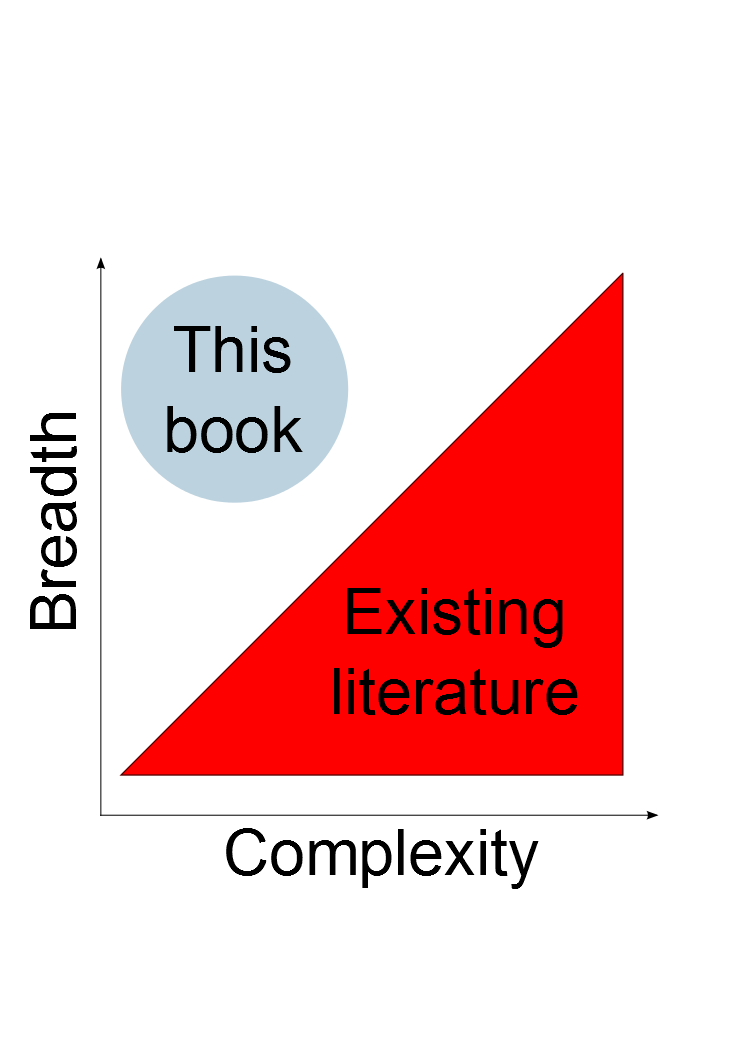
\includegraphics{HowToUse_existingLiterature.png}}
\caption{The aim of this book.}\label{fig:HowToUse_existingLiterature}
\end{figure}


\section{Who is this book for?}
This book is for anyone who has ever tried, and \textbf{failed} at statistics, and particularly, Bayesian statistics.

The text is aimed at anyone who has completed high school mathematics, and wants to conduct Bayesian inference on real world data. We assume no previous knowledge of probability\footnote{Which is central to Bayesian analysis.}, and devote the entirety of chapter \ref{chap:Probability} to this purpose. We do not require that the student is versed in classical statistics, as we aim to build an alternative, and complementary path to a shared goal. As such, after chapter \ref{chap:subjectiveFrequentistBayes}, we will not give too much attention to comparisons between these two approaches.

Whilst we start at the very beginning of statistical inference, we aim to provide a guide which will be of practical-use for a large proportion of analyses that are likely to be encountered in real life.

\section{Pre-requisites}
Knowledge of the following is strongly recommended, in order to allow the reader to grasp all that is contained within this text:

\begin{itemize}
\item \textbf{Algebra:} manipulation of symbolic expressions is widespread throughout the text.
\item \textbf{Summations:} mainly used for writing down likelihood functions.
\item \textbf{Calculus:} mainly integration, although there are sprinklings of differentiation in places.
\end{itemize}

The only other pre-requisite is more to do with the practical application of Bayesian analysis: a knowledge of the statistical software \textit{R}\cite{RLanguage} would be \textit{useful}. We do not classify this item with those above, partly because we aim to only use very basic functioning in this language, and partly because we will explain those examples thoroughly. This language is widely-used for statistical analysis, and because of its popularity there are many excellent online introductions to this language, which are freely available:

\begin{itemize}
\item \url{www.coursera.org} - there are a number of great lecture courses with associated problem sets available for learning R here. In particular, the courses by Roger Peng at John Hopkins are very worthwhile.
\item \url{http://tryr.codeschool.com} - a short interactive introductory lesson on the basics of R. 
\item \url{www.datacamp.com/courses/free-introduction-to-r} - 4 hours of interactive lectures on the basics of R.
\item \url{http://cran.r-project.org/doc/contrib/Owen-TheRGuide.pdf} - a nice written guide to R.
\end{itemize}

Whilst none of these are essential, if you have difficulty in following the examples in this text, then we recommend that you have a look at the above resources.

\section{Book outline}
We have written this text to make each chapter as self-contained as is possible. Whilst, at times, the reader may feel that this focus on modularity means that some elements reoccur, this is intended not to make reading repetitious, or worse \textit{boring}! It is for two purposes: to aid the aforementioned compartmentalisation; and because we believe that some ideas are worth encountering, and re-encountering, at different points in your pursuit of knowledge.

The book is divided into five \textit{Parts}:

\begin{itemize}
\item \textbf{Part} \ref{part:BayesianInferenceIntro}\textbf{: An introduction to Bayesian inference.} 
\item \textbf{Part} \ref{part:bayesianFormula}\textbf{: Understanding the Bayesian formula.}
\item \textbf{Part} \ref{part:analyticalBayes}\textbf{: Analytic Bayesian methods.}
\item \textbf{Part} \ref{part:computationalBayes} \textbf{: A practical guide to doing real life Bayesian analysis: Computational Bayes.}
\item \textbf{Part} \ref{part:regressionHierarchical} \textbf{: Regression analysis and hierarchical models.}
\end{itemize}

Part \ref{part:BayesianInferenceIntro} firstly provides an introduction to the purpose of statistical inference, then goes on to compare and contrast the Bayesian and classical approaches to this problem. Bayesian inference is based on probability. Hence it is imperative to understand how to manipulate these types of mathematical object. The latter half of this part is thus devoted to exactly this purpose. Part \ref{part:bayesianFormula} introduces the reader to the constituent elements of the Bayesian inference formula, and in doing so provides an all-round introduction to the practicalities of doing Bayesian inference. Part \ref{part:analyticalBayes} aims to equip the user with the knowledge of the most practically-relevant probability distributions for Bayesian inference. These objects come under two categories in general\footnote{although some distributions fall into both}: prior distributions, and likelihood distributions. Knowledge of these distributions is essential for understanding existent research papers, and books which use Bayesian statistics, as well as to conduct Bayesian inference in the first place. The rest of the part is concerned with introducing the reader to 'nice' combinations of distributions which allow for a pen-and-paper deduction of quantities of interest. This is important not only as a stepping stone to computational methods, but also because these places are often a good place to start before implementing more nuanced models. Part \ref{part:computationalBayes} introduces the reader to the modern methods of undertaking Bayesian analysis; through computational Markov Chain Monte Carlo. This part aims to provide an intuitive introduction to some of the most important algorithmic tools used in computational methods. It also importantly introduces the reader to the statistical languages covered in this text: \textit{Stan} and \textit{JAGS}. This part is essential reading for anyone wanting to conduct serious real world Bayesian analysis of data. Part \ref{part:regressionHierarchical} builds on the previous part, and introduces the reader to the most important aspect of Bayesian modelling; hierarchical models. It also provides an in-depth introduction to doing Bayesian regression modelling.

Each chapter has two introductory summaries: the \textit{chapter mission statement}, and \textit{chapter goals}. The former is usually a one or two sentence gist of the material to be covered in the following chapter, as well as the learning outcomes of the section. The \textit{chapter goals} section is more detailed, and links together material encountered in previous chapters, and provides more of a narrative on the position of the particular chapter in question in a journey to understand Bayesian statistics. 

The \textit{chapter summary} sections at the end of each chapter provide the reader with a description of the skills acquired within, as well as some perspective on the material's position within the book's overall goals. The \textit{chapter outcomes} section provides a check-list of the skills acquired within the chapter. 

\section{Route planner - suggested journeys through Bayesland}
Ben note to self: \textbf{Change this to make of the same tick and cross table format as that of the Bayesian machine learning book!}

In the style of most good guide books, we provide itineraries through the area in question. These journeys are meant to be shortish paths towards gaining a better understanding of particular elements of Bayesian statistics, although as most trips are, they are not as all-encompassing, as a more prolonged stay. We provide the following trips through Bayesland, based on time, goals, and pre-requisite knowledge:

\begin{itemize}
\item \textbf{The long-weekender (introductory):} chapter \ref{chap:subjectiveFrequentistBayes} introduces you to the theory behind statistical inference, as well as providing a gentle introductory comparison between Bayesian and classical approaches. If you have extra time, and some knowledge of handling probability distributions, then skip ahead to chapter \ref{chap:posterior}.
\item \textbf{The two week basic trip (introductory):} Part \ref{part:BayesianInferenceIntro} and Part \ref{part:bayesianFormula} provide a full introduction to Bayesian statistics, from the ground up. 
\item \textbf{The two week refresher (medium):} Read chapter \ref{chap:subjectiveFrequentistBayes} to get your bearings. Dependent on your knowledge of the Bayesian formula Part \ref{part:bayesianFormula} can either be read, or left behind. Part \ref{part:analyticalBayes} should be read almost in full, as this will get you up to speed with many of the tools necessary to understand many research papers. However, you may be able to 'get away' without reading chapter \ref{chap:ObjectiveBayes} on Objective Bayes.
\item \textbf{The two week full practical swing (medium-master):} If you are happy with your knowledge of the Bayesian inference formula, as well as the distributions used in Bayesian analysis, then you may want to skip ahead to Part \ref{part:computationalBayes}, which introduces computational methods. This introduces the reader to both \textit{Stan} and \textit{JAGS} which are the statistical languages used in this text to carry out Bayesian analyses. If you have time, and are willing, then you may want to progress to Part \ref{part:regressionHierarchical}. 
\item \textbf{The 'I need to do Bayesian analysis' now three day leg (medium-master):} This is a tailor-made trip suited to those practitioners who need to carry out Bayesian data analysis \textit{fast}. The most likely people here are those in research: either academic or corporate; who have an existing knowledge of Bayesian statistics. Skip ahead to Part \ref{part:computationalBayes}, and read the chapter on \textit{Stan} (if your analysis only contains a few discrete variables), or \textit{JAGS} (if your analysis contains a number of discrete parameters). You may then want to use the index to look for the most relevant sections, although Part \ref{part:regressionHierarchical} will be your main point of reference.
\item \textbf{A theoretic and practical journey through modern Bayesian analysis (medium-master):} You want to learn as much about applied Bayesian methods as time will allow, but you also want to gain some practice in practically doing Bayesian statistics. Read all of Part \ref{part:computationalBayes}.
\item \textbf{A two week modelling masterclass (master):} you know all the basics, and are acquainted with the use of either \textit{Stan} or \textit{JAGS, BUGS}. You want to see these applied to carrying out real life data analysis. Read all of Part \ref{part:regressionHierarchical}. 
\end{itemize}

\section{Video}
Whenever the reader sees the following signpost, there is a video available to supplement the main text:

\boxed{Video:}

By following the web address indicated, the user can watch the video on YouTube.

The videos are not meant to replace the reading of the text. They are supplementary, and aim to address topics through alternative approaches, and with different examples.

Ben note to self:\textbf{It might be good to provide a link to a real video here.}

\section{Interactive elements}
Whenever the reader sees the following signpost, there is an interactive element available to supplement the main text:

\boxed{Interactive:}

By following the web address indicated, the user can dynamically interact with these examples, by clicking, entering numbers, or moving slider bars. It is hoped that these elements in particular, will allow the user to build up an intuition behind Bayesian theory, which is essential for doing real world analysis.

These elements have been created using Mathematica, although there is no need to own the software in order to play. 

\section{Interactive problem sets}
The reader can practice their knowledge using the problem sets at the end of each chapter. The problem sets are \textbf{interactive}, and are of the form used in many online education systems. The student can submit their answers to a selection of the questions, and will receive a mark out of 100 for each problem set.

The problems available aim to cover mainly practical application of Bayesian data analysis, although there are also sections which are more theoretic in nature.

For teachers of the subject, there are parts of each problem set which are not interactive, and can be used as a part of a taught course.

\section{Code}
Whenever appropriate, particularly in Part \ref{part:computationalBayes} onwards, we will include snippets of code in Stan, JAGS and R. These are commented thoroughly, which should be self-explanatory. They aim to be as self-contained as space allows.

\section{R, Stan and JAGS}
Modern Bayesian data analysis uses computers. Luckily, for the student of Bayesian statistics, the most up-to-date and useful software packages are open source; meaning they are freely available to use. In this book we solely use this type of software, so prevent the student needing to spend more on acquiring them.

The most recent, and powerful software to emerge is that developed by Andrew Gelman et al.\cite{stan-software:2014} and is called \textit{Stan}. The language of this software is not difficult to understand, and easier to write and debug than its competition. Stan allows a user to fit complex models to data sets, without having to wait an age for the results. With updates planned to this software, which will make it even more powerful, and user-friendly, this is without question the most appropriate software on which to conduct Bayesian analysis.

Ben note to self: Dependent on when the book is released, we may remove the following section, since Stan may allow for discrete sampling directly by then.

The only snag with Stan is that because of the particular type of engine under the hood, it is not possible to directly use it to conduct analysis for discrete parameters. As we shall see in Part \ref{part:computationalBayes}, this issue can be sidestepped in Stan, but for some circumstances it is easier to write the model using another piece of software called \textit{JAGS}\cite{plummer2003jags}. This language is slightly different to write, and in nature to that of Stan. We will explain its functioning in detail in Part \ref{part:computationalBayes}, and walk though a number of introductory examples, however we advocate using this software only in circumstances where it is simpler to implement than a corresponding model in Stan.

The two aforementioned statistical languages are usually run through another piece of 'helper' software. Whilst there are a number of alternatives here, particularly for Stan, we choose to use \textit{R} here. This is because this software is both open source, and widely used. The former means that anyone with a modern computer should be able to get their hands dirty in Bayesian analysis; the latter is important since the code base is well-maintained and tested.

\section{Why don't more people use Bayesian statistics?}
Many are discouraged from using Bayesian approaches to analysis due to its supposed difficulty, and dependence on mathematics. However, we would argue that this is, in part, a weakness of the existent literature on the subject, which this book looks to address. It also highlights how many books on classical statistics sweep their inherent complexity and assumptions under the carpet, resulting in texts which are easy to digest; meaning that for many the path of least resistance is to forge ahead with classical tools. 

By its dependence on the logic of probability, this means on first glances, Bayesian statistics appears more mathematically-complex. However, what is often lost in introductory texts on Bayesian theory, is the intuitive explanations behind the mathematical formulae. In this text instead, we shift the emphasis towards the latter; choosing to focus on graphical and illustrative explanations rather than getting lost in the details of the mathematics, which to be honest, is not necessary for much of modern Bayesian analysis. We hope that by doing so, we shall lose fewer casualties to mathematical complexity, and redress the imbalance between classical and Bayesian analysis applications.

Again, on first appearances, the concept of the \textit{prior} no doubt leads many to 'abandon ship' early on the path to understanding better Bayesian methodologies. However, we will cover this concept in detail in chapter \ref{chap:Prior} which is fully-devoted to this subject, we hope to banish this particular thorn in the side of would-be Bayesian statisticians.

The reliance on computing, in particular simulation, is also seen to add to the complexity of Bayesian approaches. Whilst, this is true, we argue that the modern algorithms used for simulation are straightforward to understand, and with modern software, easy to implement. Furthermore, the added complexity of simulation methods is more than compensated by the straightforward extension of Bayesian models to handle arbitrarily complex situations. Like most things worth learning, there is a slight learning curve to become acquainted with the languages used to write modern Bayesian simulations. However, we hope to make this curve sufficiently shallow by incremental introduction of elements used in these computational applications.

\section{What are the tangible (non-academic) benefits of Bayesian statistics?}
In Bayesian textbooks much discourse is devoted to advocating the academic reasons for choosing to use a Bayesian analysis over classical approaches. However, often authors neglect to promote the more tangible, everyday benefits of the former. Here, we list the following \textit{real} benefits of a Bayesian approach:

\begin{itemize}
\item \textbf{Simple and intuitive model testing and comparison}. The prior- and posterior-predictive distributions allow for in-depth testing of any particular aspect of a model, by comparing it with the same aspects from the data collected. The Bayesian approach also provides a logical framework in which to compare different models.
\item \textbf{Straightforward interpretation of results.} In classical analyses, the \textit{confidence interval} is often taken to be a measure of uncertainty for a particular parameter. As we shall see in section \ref{sec:Posterior_classicalConfidenceInterval}, this is not the case, and interpretation of this concept is not straightforward. By contrast Bayesian \textit{credible intervals}, can be taken to be a measure of uncertainty in a parameter, as they are obtained directly from probability distributions.
\item \textbf{Full model flexibility}. Modern Bayesian analyses use computational simulation in order to carry out analyses. Whilst this might appear excessive when compared to classical approaches, an additional benefit is the straightforward extension to almost arbitrarily complex models when using Bayesian approaches. This means that Bayesian models can be extended to encompass any complexity of data process. This is in contrast to classical approaches, where the intrinsic difficulty of analysis scales with the complexity of the model chosen.
\item \textbf{The best predictions.} Leading figures both inside and outside of academia use Bayesian approaches for prediction. An example being Nate Silver's correct prediction of the 2008 US Presidential election results \cite{silver2012signal}.
\end{itemize}

\section{Suggested further reading}
A good book should leave the reader wanting more. Due to the finiteness of this text, we recommend the following books, articles and websites. These aren't necessarily all on Bayesian statistics, but fall under the wider categories of statistical inference and learning. We also provide a score of the complexity of reading these texts, which may guide your choice:

\begin{itemize}
\item \textbf{Bayesian Data Analysis (medium-master): } A masterpiece produced by the master statisticians Andrew Gelman, and Donald Rubin amongst others. This is the most all-encompassing, and up-to-date text available on applied Bayesian data analysis. There are plenty of examples of Bayesian analysis applied to real world data, and are well-explained\cite{gelman2013bayesian}.
\item \textbf{Data Analysis Using Regression and Multilevel/Hierarchical Models (medium): } Another belter from Andrew Gelman, along with his co-author Jennifer Hill. This takes the reader through numerous examples of regression modelling, and hierarchical analysis. The text is not solely constrained to Bayesian analysis, and covers classical methods as well.
\item \textbf{Mastering metrics (introductory): } A great, back-to-basics, book on causal inference by the masters of econometrics Josh Angrist and Jörn-Steffen Pischke. This is an exhibition of the five main methods used to conduct causal inference in the social sciences: regression, matching, instrumental variables, differences-in-differences, and regression discontinuity design. This is a very readable text, and suitable for anyone wanting to learn about policy evaluation.
\item \textbf{Mostly Harmless Econometrics (master-of-metrics): } Again by Josh Angrist and Jörn-Steffen Pischke. A thorough, and mathematically detailed text which takes the reader through most of those methods used in causal inference today. Its small size is deceptive, and is not one to read over a single weekend. However, it is well worth persisting with this book, as the nuggets that await the determined reader are worth their weight in gold. Also see Gelman's review of this book, which provides an interesting critique of the text.
\end{itemize}

\part{An introduction to Bayesian inference}\label{part:BayesianInferenceIntro}
\section{Part mission statement}
The purpose of this Part is twofold: firstly to introduce the reader to the principles of inference; secondly to familiarise them with knowledge of how to manipulate probability distributions, which is essential to Bayesian inference.

\section{Part goals}
Both Frequentist and Bayesian inferential processes aim to assess the evidence for a particular hypothesis after we have obtained a particular data sample. However, it is usually much easier to obtain the inverse - the probability of the data given the hypothesis. Thus in order to obtain the desired quantity, a process of \textit{inversion} is required, which is central to all statistical inference. There are currently two predominant viewpoints which approach this inversion differently: Frequentists use a rule of thumb, which has historically been agreed upon as a useful way of carrying out this process; by contrast Bayesians use Bayes' rule - the only method consistent with the logic of probability. Chapter \ref{chap:subjectiveFrequentistBayes} fully introduces the reader to the aims of statistical inference, along with the differences in philosophy and approach taken by Frequentists and Bayesians to this shared goal. 

One of the main differences in approach is the Bayesian insistence on describing everything of interest using probability distributions. The resultant theory is more elegant, as well as being more practically useful, than that proposed by Frequentists. However, in order to appreciate this elegance, it is necessary to have a good working knowledge of probability distributions, and their manipulations. Hence chapter \ref{chap:Probability} provides a fully introductory course on probability distributions. 

\chapter{The subjective worlds of Frequentist and Bayesian statistics}\label{chap:subjectiveFrequentistBayes}
\section{Chapter mission statement}
At the end of this chapter, the reader will understand the purpose of statistical inference; importantly recognising the similarities and differences between Frequentist and Bayesian inference. We then go on to introduce the most important theorem in modern statistics: \textit{Bayes' rule}.
 
\section{Chapter goals}
In life, we are often tasked with building predictive models to understand complex phenomena. As a first approximation, we often disregard parts of the system, which are not directly of interest; making the models \textit{statistical} rather than deterministic. There are two distinct approaches to statistical modelling: Frequentist or Classical inference, and Bayesian. This chapter will explain the similarities between these two approaches, and importantly, indicate where they differ substantively. It is typically fairly straightforward to calculate the probability of obtaining different data samples, if we assume that we \textit{know} the process that is responsible for generating these data in the first place. However, we normally do not know these processes with certainty, and it is the goal of statistical inference to derive estimates of the unknown characteristics, or \textit{parameters}, of these mechanisms. Bayesian statistics allows us to go from what is known - the \textit{data} - to extrapolate backwards in order to make probabilistic statements about the overriding parameters which were responsible for its generation. This inversion process is carried out in Bayesian statistics by application of Bayes' rule, which will be introduced in this chapter.  It is important to have a good understanding of this rule, and we will spend some time, throughout this chapter and Part \ref{part:bayesianFormula}, developing an understanding the various constituent components of the formula.

\section{Bayes' rule - allowing us to go from the effect back to its cause}\label{sec:Intro_bayesCauseEffect}
Suppose we knew that a casino was crooked, and uses a die with a probability of rolling a 1 that is twice that of its unbiased value. We could then calculate the probability that we roll two 1s in a row:

\begin{align}\label{eq:Intro_crookedCasinoBayes}
Pr(1,1) &= \frac{1}{3} \times \frac{1}{3}\\
&= \frac{1}{9}
\end{align}


Here we use 'Pr' to denote a probability, with the comma here having the literal interpretation of 'and' - hence $Pr(1,1)$ is the probability we obtain a 1 on the first roll, \textit{and} a 1 on the second. The probability of $\frac{1}{3}$ is twice that of the unbiased probability: $Pr(1) = 2\times\frac{1}{6} = \frac{1}{3}$. Do not worry if you don't understand fully this calculation, as we will devote the entirety of the next chapter to working with probabilities.

In this case we have presupposed a \textit{cause} - the casino being crooked - in order to derive the probability of a particular effect - rolling two consecutive 1s. In other words we have calculated $Pr(effect|cause)$. The vertical line, $|$, here means \textit{given} in probability (Again do not worry if you don't understand this notation, as we will devote the entirety of chapter \ref{chap:Probability} to developing an understanding of probability and its notations.) 

Until the latter half of the 17th Century, probability was most frequently used as a method to calculate gambling odds; similar in nature to that shown in (\ref{eq:Intro_crookedCasinoBayes}). It was viewed as a dirty subject, not worthy of the attention of the most esteemed mathematicians.

However, the arrival of the Reverend Thomas Bayes, and slightly later and more famously, Laplace \footnote{See \cite{mcgrayne2011theory} for an interesting history of Thomas Bayes and Laplace, as well as a history of the use of Bayes' theorem.} started a change in this perspective. They realised that it is possible to move in the opposite direction - to go from effect back to cause:

\begin{equation}
Pr(effect|cause) \xrightarrow{Bayes' theorem} Pr(cause|effect)
\end{equation}

In order to take this leap however, it was necessary to create/discover a rule, which later became known as Bayes' rule/theorem. This can be written:

\begin{equation}\label{eq:Intro_BayesRuleCauseEffect}
Pr(cause|effect) = \frac{Pr(effect|cause)\times Pr(cause)}{Pr(effect)}
\end{equation}

In the casino example, this formula tells us how to 'invert' the original probability $Pr(1,1|crooked\;casino)$ to get the thing in which we are probably more interested as a patron of said casino $Pr(crooked\;casino|1,1)$. In words, what is the probability that the casino is crooked, \textit{given} that we rolled two 1s. We will not show how to carry out this calculation in practice now; delaying this until we have learned about probability in chapter \ref{chap:Probability}.

Bayes' rule is central to the Bayesian approach to statistical inference. However, before we introduce Bayesian inference, we first need to explain the purpose of inference!

\section{The purpose of statistical inference}\label{sec:Intro_purposeStatisticalInference}
How much does a particular drug contribute to treatment success? What can an average student earn after obtaining a college education? Will the Democrats win the next US Presidential election? In life we often want to test theories, then go on to draw conclusions.

However, it is often impossible to exactly isolate the parts of a system which we want to examine. The outcome of history is hence determined by a nexus of interacting elements; each of which contributes to the reality that we witness. In the case of a drug trial, we may not be able to control the diets of participants, and are certainly unable to control for their idiosyncratic metabolisms, both of which could impact the results we see. Evaluating the return to a college education - there are a range of factors which affect the wage which an individual ultimately commands, of which education is only one element. The outcome of the next US Presidential election depends on party politics, the performance of the incumbent government, as well as the media's portrayal of the candidates. 

In life noise obfuscates the signal. The wind, rain, snow and sleet make it difficult to forge a path to where we want to go.

Statistical inference allows us to draw conclusions in this blustery landscape; separating the signal from the noise. It is the logical framework which we can use to trial our beliefs against \textit{data}. 

In statistics, we formalise our beliefs in models of \textit{probability}. The models are probabilistic because we assume we are ignorant to many of the multitude of interacting parts of a system, meaning we cannot say with certainty whether something will, or will not, occur.

Suppose we are evaluating the efficacy of a drug in a trial. We might suppose that \textit{on average}, the drug might have a given probability of working as desired. However, before we carry out any trials, we are unaware of its exact treatment success rate. Fortunately, statistical inference allows us to estimate this unknown characteristic, or \textit{parameter}, from the data we are given. 

There are now two predominant schools of thought for carrying out this process of inference: \textit{Frequentist} and \textit{Bayesian}. Although this book is devoted to the latter, we now spend some time comparing the two approaches, so that a reader is aware of the different paths taken to their shared goal.

\section{The world according to Frequentists}\label{sec:Intro_FrequentistsWorld}
In Frequentist or classical statistics, we suppose that our sample of data is the result of one of an infinite number of exactly-repeated experiments. The sample we see in this context is hence assumed to be the outcome of some probabilistic process. Any conclusions that we draw from this approach are based on the supposition that events occur with probabilities, which represent long-run frequencies. 

For example, if we flip a coin, we might assume that any sequence of outcomes we obtain is indicative of results we'd get if we were to conduct the experiment an infinite number of times. Further, we might take the proportion of heads observed in this infinite set of throws as defining the probability of obtaining a 'heads'. We suppose that this probability actually exists, and is fixed for each set of coin-throws that we carry out (see figure \ref{fig:Intro_FrequentistBayesProbability}).

In general, in Frequentist statistics assume that the data is \textit{random} and results from \textit{sampling}, from a fixed and defined \textit{population} distribution. For a Frequentist the noise that obscures the true signal of the population relationship in which we are interested is due to \textit{sampling variation}; the fact that the sample that we pick will each time be slightly different, and not exactly representative of the population. 

We may flip our coin 10 times, obtaining 7 heads even if the long-run proportion of heads is $\frac{1}{2}$. To a Frequentist, this is because we have picked a slightly odd sample from the population of infinitely-many repeated throws. Further, if we flip the coin another 10 times, we will likely get a different result, because we have picked a different sample.

\begin{figure}
\centering
\scalebox{0.3} 
{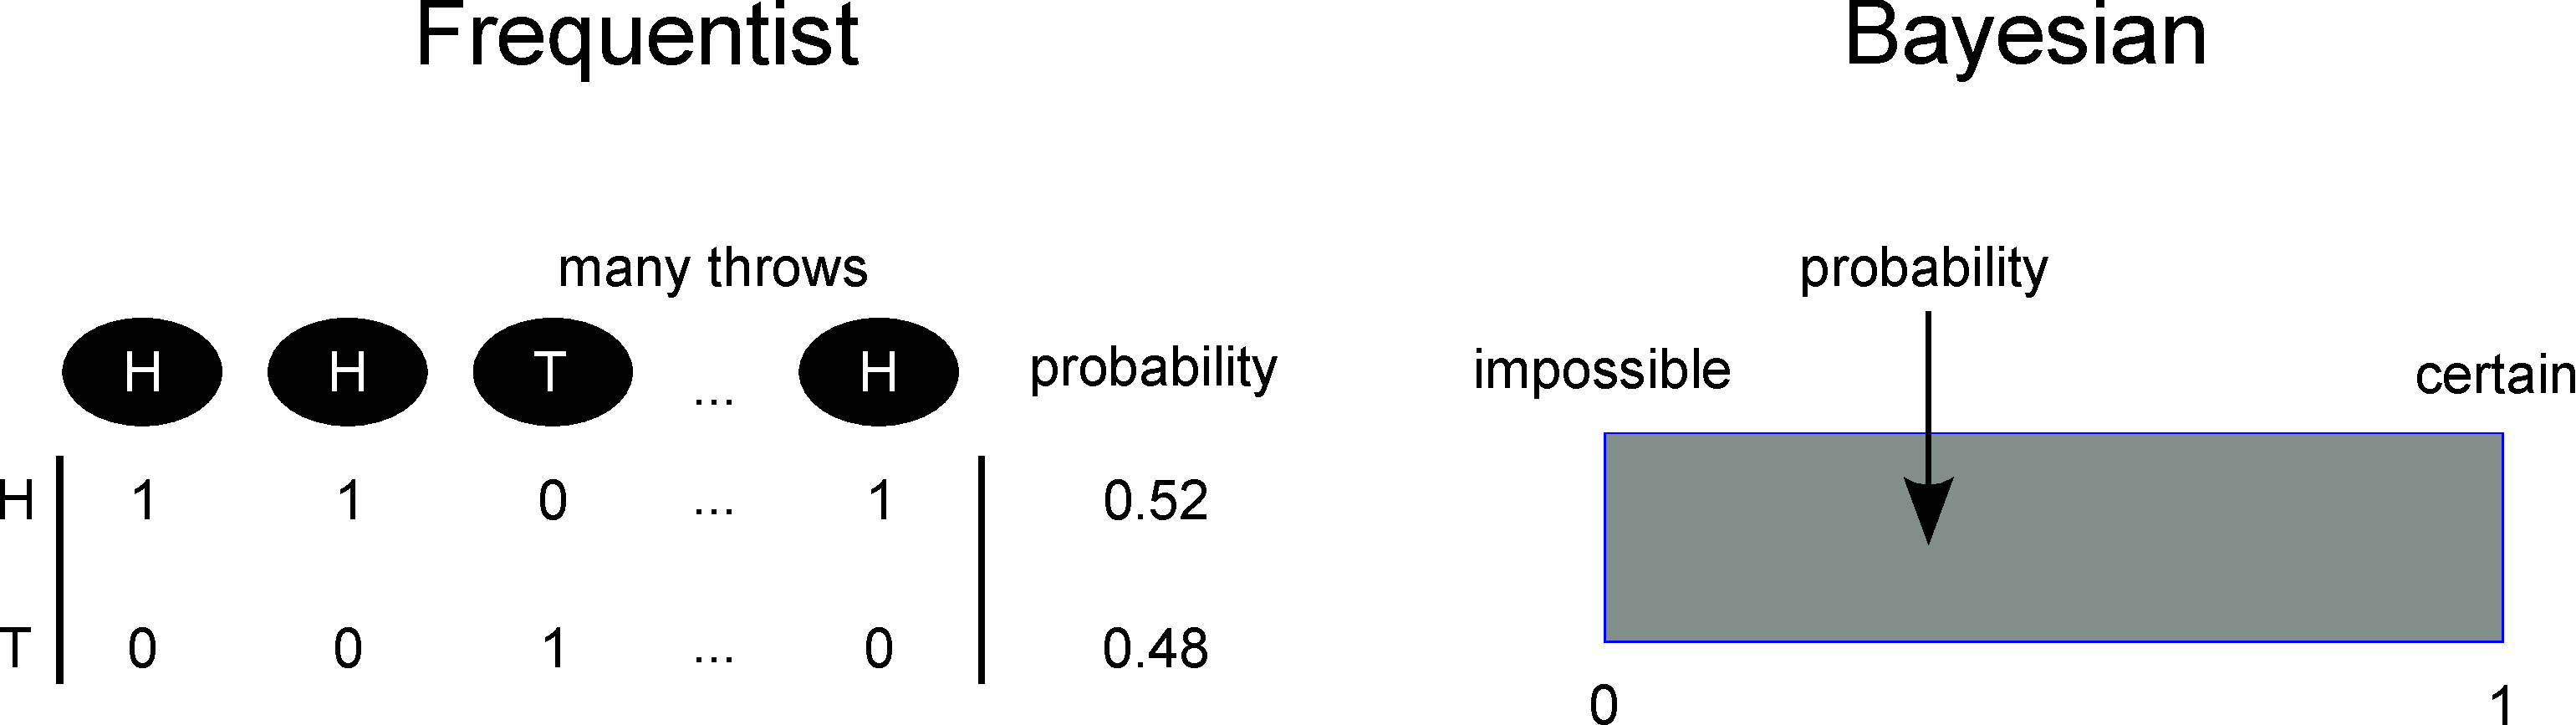
\includegraphics{Intro_FrequentistBayesProbability.pdf}}
\caption{The Frequentist and Bayesian approaches to probability.}\label{fig:Intro_FrequentistBayesProbability}
\end{figure}

\section{The world according to Bayesians}
Bayesians do not imagine repetitions of an experiment in order to define and specify a probability. It is merely taken as a measure of certainty of a particular belief. From this viewpoint, the probability of us throwing a 'heads' measures and quantifies our underlying belief, that before we flip the coin, it will land this way. 

In this sense, Bayesians do not view probabilities as concrete entities that actually exist. They are merely abstractions which we can use to help express our uncertainty. In this frame of reference there is no necessity for events to be repeatable in order to define a probability. We are thus equally able to say, 'The probability of a heads is 0.5', or, 'The probability of the democrats winning the 2020 US Presidential election is 0.75'. Probability is merely seen as a scale from: 0 where we are certain an event will not happen, to 1 where we are certain it will (see figure \ref{fig:Intro_FrequentistBayesProbability}). 

A statement such as 'The probability of the democrats winning the 2020 US Presidential election is 0.75' is hard to explain using the Frequentist definition of a probability. There is only ever one possible sample - the history that we witness - and what would we actually mean by a 'population of all possible US elections which happen in the year 2020'? 

Probabilities are therefore seen as an expression of subjective beliefs, meaning they can be updated in light of new data. The formula invented by the Reverend Thomas Bayes provides the \textit{only} logical manner in which to carry out this process, and is central to Bayesian inference, where we aim to express probabilistically our uncertainty in parameters after we have seen the \textit{data}. 

Bayesians assume, since we are witness to the data, that it is \textit{fixed}, and therefore does not vary. We do not need to imagine that there are an infinite number of possible samples. We 'see' our data, and hence do not need to view it as the undetermined outcome of some random process.

In contrast, we do not ever learn exactly the value of an unknown parameter. This epistemic uncertainty means that in Bayesian inference we choose to view the parameter as a quantity that is probabilistic in nature. We can view this in one of two perspectives. Either we view the unknown parameter as truly being \textit{fixed} in some absolute sense, but our beliefs are uncertain, and thus probabilistic. Alternatively, we can take the view that there isn't some definitive \textit{population} process, and for each sample we take, we get a slightly different parameter.

In the latter perspective we get different results from the coin flipping because each time we are subjecting our system to a slightly different probability of it landing 'heads' up. This could be because we mildly altered our throwing technique, or started with the coin in a different position. In the former perspective, we view the sample as a noisy representation of the signal, and hence we get different results for each set of throws. Although these two descriptions are different philosophically, they are not mathematically, meaning we can apply the same analysis to both.

\section{Frequentist and Bayesian inference}
The Bayesian inference process is the only logical and consistent way to modify our beliefs to take into account new data. We start out before we collect data with a probabilistic description of our beliefs, which we call a \textit{prior}. We then collect data, and together with a model describing our theory, Bayes' formula for probability allows us to calculate our post-data or \textit{posterior} belief:

\begin{equation}
prior + data \xrightarrow{model} posterior
\end{equation}

Ignore for the moment that we have not explained was is meant by this mysterious \textit{prior}, as we shall introduce this element properly in section \ref{sec:Intro_priors}. 

In Bayesian inference, we want to draw conclusions based on purely probabilistic descriptions of phenomena. If we wish to summarise our evidence for a particular hypothesis, we describe this probabilistically, as the 'probability of the hypothesis \textit{given} the data obtained'. 

The difficulty in obtaining this type of conclusion is that when we write down a probability model describing the situation under examination, we can only use it to compute the 'probability of obtaining our data \textit{given} our hypothesis being true'; the inverse of that which we desire. This probability is calculated by taking into account all the possible samples that we could have obtained from the population, if we assume the hypothesis is true. The issue of statistical inference, common to both Frequentists and Bayesians, is to how to invert this probability to get the desired quantity of interest.

Frequentists stop here, using this probability as evidence for a particular hypothesis in question. They assume a hypothesis to be true, and on this basis calculate the probability of obtaining a data sample as extreme as the one obtained. If this probability is small, then it is assumed that it is unlikely that the hypothesis is true, and is rejected. Note however if we reject a hypothesis, we have no way of telling whether it is true, and we just witnessed a weird sample, or that it is actually false. Also, note that in this inference process, we have also had to imagine obtaining a sample more extreme than our result, in order to get a usable probability. 

Bayes' formula allows us to circumvent these difficulties, by inverting the Frequentist probability to get the 'probability of the hypothesis given the \textit{actual} data we obtained'. There is no need for an arbitrary cut-off in the probability in order to validate the hypothesis; all information is summarised in this probability, and hence can be viewed as the end point of an analysis in itself.

\begin{figure}
\centering
\scalebox{0.4} 
{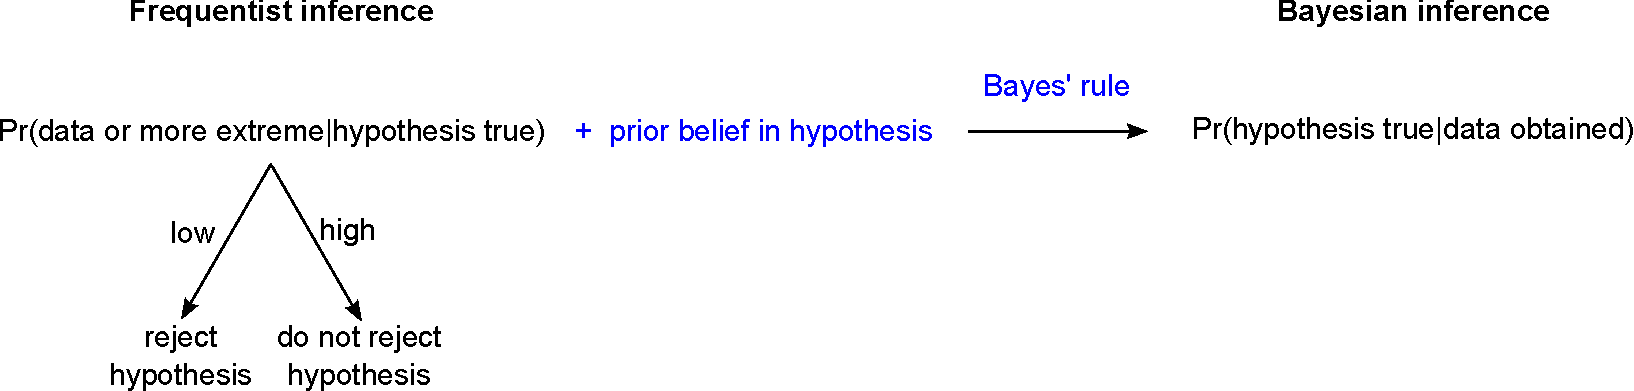
\includegraphics{Intro_BayesVsFrequentist.pdf}}
\caption{Frequentist and Bayesian inference.}\label{fig:Intro_BayesVsFrequentist}
\end{figure}

The next few, albeit silly, and (more than) somewhat contrived examples, illustrate a difference both in methodology, but perhaps more significantly, in philosophy, between the two different approaches.

\subsection{The Frequentist and Bayesian murder trials}
Assume you find yourself in the unfortunate situation where you are (hopefully falsely) accused of murder, and face a trial by jury. A variation in the usual tale is that you personally have a choice over the method used by the jury to assign guilt: either Frequentist or Bayesian. Another unfortunate twist is that the legal system of the country starts by presuming \textit{guilt} rather than \textit{innocence}.

Let's assume that you have been shown by a security camera to have definitely been in the same house as the victim - Sally - on the night of her demise. 

If you choose the Frequentist trial, your jurors start by coming up with a model based on previous trials, which assigns a probability of you being seen by the security camera if you were guilty. They then use this to make the statement that, 'If you did commit the murder, then 30\% of the time you would have been seen by the security camera', based on a hypothetical infinity of repetitions of the same conditions. Since this is not sufficiently unlikely (the p value is not below 5\%), the jurors cannot reject the null hypothesis of \textit{guilt}, and you are sentenced to life in prison.

In a Bayesian trial, the jury are first introduced to an array of evidence, that suggests that you neither knew Sally, nor had any previous record of violent conduct; being otherwise a perfectly respectable citizen. Furthermore, the ex-boyfriend of Sally is a multiple-violent-offending convict on the run from prison after being sentenced by a judge on the basis of witness testimony by Sally. On this basis, the jury determine a \textit{prior} probability in the hypothesis that you are guilty that is $\frac{1}{1000}$\footnote{Do not worry that we are yet to explain how one can construct priors, since we shall devote the entirety of chapter \ref{chap:Prior} to this purpose.}. They then use the same model as the Frequentists, to determine that the probability of you being seen by the security camera given your guilt is 30\%. However, they then coolly use Bayes' rule (we will introduce this concept in section \ref{sec:Intro_bayesCauseEffect}), and conclude that the probability of you committing the crime is $\frac{1}{1000}$ (see section \ref{sec:Intro_appendixMurder} for a full description of this calculation). Based on this evidence, the jury acquits you, and you go home to your family.

\subsection{Radio control towers: example}
In a hypothetical war two radio control workers sit side-by-side, Mr Pearson (from frequentland), and Mr Laplace (from the county of Bayesdom), and are tasked with finding an enemy plane that has been spotted over the country's borders. They will each feed this information to the nearest airforce base(s) which will respond by sending up aircraft of their own. There are however, administratively two different airforces, which correspond to the two different counties. Although the airforces of frequentland and Bayesdom share airbases, they are distinct, and only respond to Mr Pearson and Mr Laplace's advice respectively. The war, although short, has been costly to both allies, and they each want to avoid needless expenditure, as well as the unwarranted scaring of the local populace by sending up jets.

Mr Pearson starts by inputting the radar information into a computer program which uses a model of a plane's position which has been calibrated against a dataset of historical plane data in this short war. The result comes out instantly. 

"...The plane is most likely 5 miles from the town of Tunbridge Wells."

Without another moment's thought, Mr Pearson radios the base of Tunbridge Wells, telling them to scramble all 10 available Frequentist fighter jets immediately. He then gets up to get himself a well-earned coffee.

Laplace knows from experience there are three different flight paths that the enemy has used to attack previously. Accordingly, he gives these regions a high probability density in his prior for the plane's current location, and feeds this into the same computer program that Pearson used. The output this time is different. By using the optional input, the program now outputs a map with the most likely regions shown via a colour shading. There is the highest posterior density over the region near Tunbridge Wells, where Pearson radioed, although the map suggests there are two other towns which might be likely victims of the plane's bombing. Accordingly, Laplace radios to Tunbridge Wells, asking them to send up four jets, and to the other two towns, asking them to send up two jets each. At the end of this all, Laplace remains seated, tired but contented that he has done his best for his own.

The enemy bomber turned out to be approaching Berkstad, one of the towns which Laplace radioed. The Bayesdom jets intercept the encroaching aircraft, and escort it out of allied airspace. Laplace is awarded a medal in honour of his efforts. Pearson looks on jealously.

\section{Bayesian inference via Bayes' rule}
Bayes' rule tells us how to update our prior beliefs in order to derive better, more informed beliefs about a situation in light of new data. As was explained in section \ref{sec:Intro_purposeStatisticalInference}, statistical inference is concerned with estimating characteristics of interest, which we call \textit{parameters}, from a dataset that we have to hand. From this point onwards we will use, $\theta$, to represent the unknown parameter(s) which we are interested in estimating. 

The Bayesian inference process uses Bayes' rule to estimate a probability distribution over those unknown parameters, after we witness the data. Do not worry if you do not know what is meant by a \textit{probability distribution}, since we shall devote the entirety of chapter \ref{chap:Probability} to this purpose. However, it is sufficient for now to describe probability distributions as a way of representing uncertainty over unknown quantities.

The form of Bayes' rule used in statistical inference is of the form:

\begin{equation}\label{eq:Intro_bayesianFormula}
p(\theta|data) = \frac{p(data|\theta)\times p(\theta)}{p(data)}
\end{equation}

Here we use $p$ to indicate a probability distribution which may either represent probabilities, or more usually, probability densities\footnote{See section \ref{sec:Probability_densityVsMassFunctions} for a description of their distinction.}. We shall now devote the next few sections to describing, in short, the various elements of (\ref{eq:Intro_bayesianFormula}). Note these only provide a partial introduction, since we will spend the entirety of Part \ref{part:bayesianFormula} to an extensive discussion of each of its constituent components.

\subsection{Likelihoods}\label{sec:Intro_likelihoods}
Starting with the numerator on the right hand side of (\ref{eq:Intro_bayesianFormula}), we come across the term $p(data|\theta)$, which we call the \textit{likelihood}. This tells us the probability of generating the particular sample of \textit{data}, if the parameters in our statistical model were equal to $\theta$. When we write down a statistical model, we can generally calculate the probability of particular outcomes, so this is easily obtained. Imagine that we have a coin that we believe to be fair. By \textit{fair}, we typically mean that the probability of the coin falling 'heads-up' is $\theta=\frac{1}{2}$. If we flip the coin twice, we might suppose that it is reasonable to model the outcomes as independent (see section \ref{sec:Probability_independence}), and hence we can calculate the probabilities of the four possible outcomes, by multiplying the probabilities of the individual outcomes together:

\begin{align}
p(HH) &= p(H)\times p(H) = \frac{1}{2} \times \frac{1}{2} = \frac{1}{4}\\
p(HT) &= p(H)\times p(T) = \frac{1}{2} \times \frac{1}{2} = \frac{1}{4}\\
p(TH) &= p(T)\times p(H) = \frac{1}{2} \times \frac{1}{2} = \frac{1}{4}\\
p(TT) &= p(H)\times p(H) = \frac{1}{2} \times \frac{1}{2} = \frac{1}{4}\\
\end{align}

Hence, if we obtained a \textit{sample} of two heads, we could write down the corresponding likelihood, $p(HH|\theta=\frac{1}{2})=\frac{1}{4}$.

Do not worry if you do not fully understand this concept, as we will be devoting an entire chapter to likelihoods in chapter \ref{chap:Likelihoods}.

\subsection{Priors}\label{sec:Intro_priors}
The next term in the numerator of the right hand side, $p(\theta)$ is the most controversial\footnote{Although this controversy is unwarranted, as we explain in section \ref{sec:Intro_implicitExplicitSubjectivity}.} part of the Bayesian formula, which we call the \textit{prior} distribution of $\theta$. It is a probability distribution which represents our pre-data beliefs as to the likely values of the parameters in our model, $\theta$. This appears at first to be slightly counter-intuitive, particularly if you are used to the world of classical statistics, which does not require us to state our beliefs \textit{explicitly} (although, we always do \textit{implicitly}, as we explain in section \ref{sec:Intro_implicitExplicitSubjectivity}.) Continuing the coin example, we might assume that we do not know whether the coin is fair or biased beforehand, so we think that all possible values of $\theta\in[0,1]$ - which represents the probability of the coin falling `heads-up' - are equally likely. We can represent these beliefs by a continuous uniform probability density on this interval (see the left-hand graph of figure \ref{fig:Intro_priors}). Normally however, we might think that coins are manufactured such that the weight distribution is fairly symmetrical on either face; meaning that we expect that the majority of coins are reasonably fair. These latter beliefs of unbiasedness could be more adequately represented by a prior of similar form to the one shown in the right-hand graph of figure \ref{fig:Intro_priors}.

\begin{figure}
\centering
\scalebox{0.6} 
{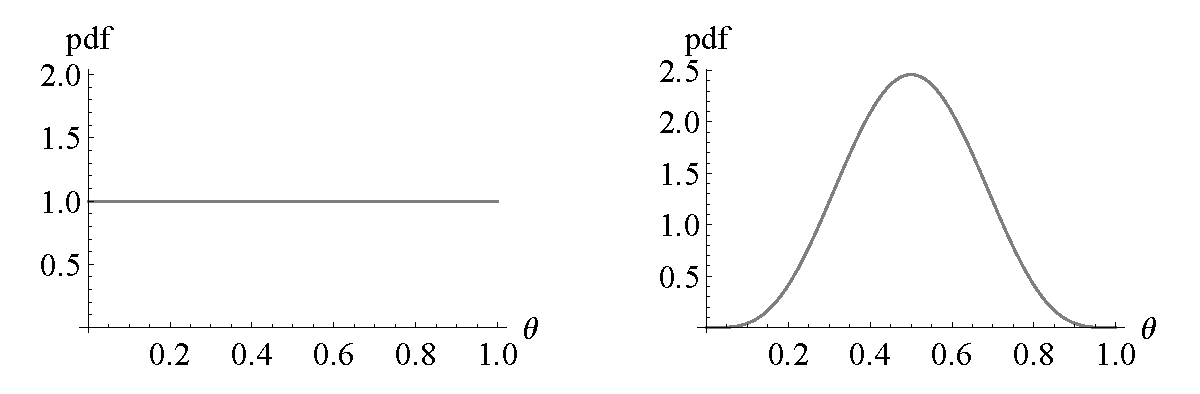
\includegraphics{Intro_priors.pdf}}
\caption{Left: All values of a the bias of a coin are equally likely. Right: It is believed that the coin is most likely fair.}\label{fig:Intro_priors}
\end{figure}

The concept of \textit{priors} will be covered in detail in chapter \ref{chap:Prior}.

\subsection{The denominator}
The final term on the right hand side, on the denominator is $p(data)$. This represents the probability of obtaining our particular sample of data, if we assume a particular model and prior. We will mostly postpone further discussion of this term until chapter \ref{chap:denominator}, when we understand better the significance of \textit{likelihoods} and \textit{priors} respectively. However, for our purposes here it suffices to say that the denominator is fully determined by choice of prior and likelihood function. Whilst it appears simple, this is deceptive, and it is partly the difficulty with calculating this term directly that leads to the introduction of computational methods of the form we will encounter in Part \ref{part:computationalBayes}.

The concept of \textit{the denominator} will be covered in detail in chapter \ref{chap:denominator}.

\subsection{Posteriors: the goal of Bayesian inference}
The posterior probability distribution $p(\theta|data)$ is often the main goal of Bayesian inference. For example, we might want to derive a probability distribution representing our post-experimental beliefs of the inherent bias, $\theta$, of a coin, \textit{given} that we flipped it 10 times, and it came up 'heads' 7 times. If we use (\ref{eq:Intro_bayesianFormula}), assuming the likelihood model specified in section \ref{sec:Intro_likelihoods} and the flat uniform prior shown in figure \ref{fig:Intro_priors}, then we would end up with a posterior distribution shown in figure \ref{fig:Intro_posterior}. Notice that the peak of the distribution occurs at $\theta=0.7$, which corresponds exactly with the percentage of 'heads' seen in the experiment\footnote{Note that if we chose a non-uniform prior, this peak would most likely shift.}. 

\begin{figure}
\centering
\scalebox{0.6} 
{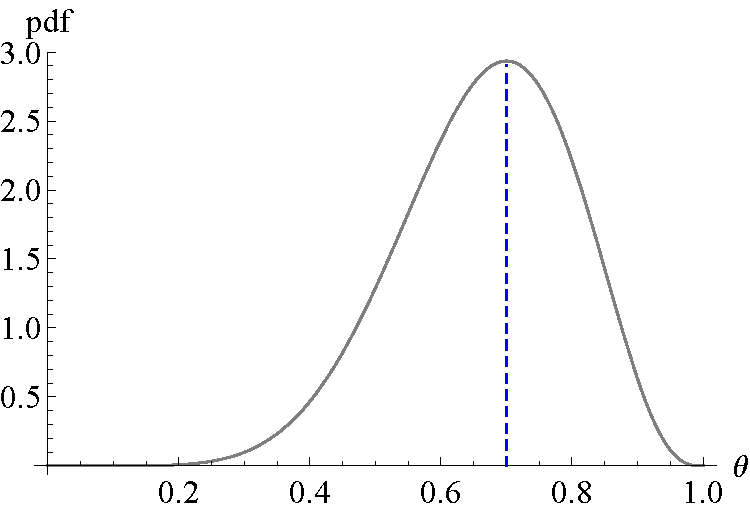
\includegraphics{Intro_posterior.pdf}}
\caption{The posterior distribution for, $\theta$, the bias of a coin when flipped, assuming a flat uniform prior and Bernoulli likelihood. We assume that 7/10 times the coin came up 'heads'.}\label{fig:Intro_posterior}
\end{figure}

The posterior distribution summarises our uncertainty regarding the value of a parameter. If the distribution is more peaked, then this emphasises that there is a greater degree of certainty with a particular value for a parameter. This increased certainty over a parameter value is frequently obtained by collecting more data. In figure \ref{fig:Intro_posteriorPeaked}, we compare the posterior distribution for the previous case of 7/10 times a coin appearing 'heads' up, with a new, larger, sample where 70/100 times the same coin comes up 'heads'. In both cases the same ratio of 'heads' to 'tails' appeared, resulting in the same peak value of $\theta=0.7$. However, in the latter case, since we have more evidence to support our claim, we end up with greater certainty over the parameter value after the experiment.

\begin{figure}
\centering
\scalebox{0.6} 
{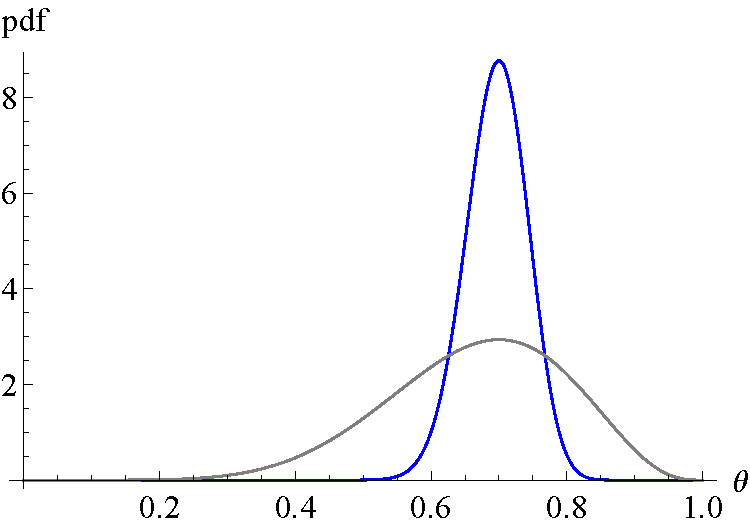
\includegraphics{Intro_posteriorPeaked.pdf}}
\caption{Posterior distributions for, $\theta$, the bias of a coin when flipped, assuming a flat uniform prior and Bernoulli likelihood. The grey line assumes that 7/10 times the coin came up 'heads'. The blue line is for the case where 70/100 times the coin came up 'heads'.}\label{fig:Intro_posteriorPeaked}
\end{figure}

The posterior distribution is also used as a starting point for prediction of future outcomes of an experiment, as well as for model testing. However, we will leave discussion of these until chapter \ref{chap:posterior}.

\section{Implicit vs Explicit subjectivity}\label{sec:Intro_implicitExplicitSubjectivity}
One of the major arguments levied against Bayesian statistics is that it is by its nature \textit{subjective}, due to its dependence on the analyst specifying their pre-experimental beliefs through \textit{priors}. This experimenter prejudice towards certain outcomes is said to bias the results away from the types of fair, objective outcomes resultant from a classical analysis. 

We argue that \textit{all} analyses involve a degree of subjectivity, which is \textit{implicitly} assumed. In a classical analysis, the statistician typically states a model for probability which depends on a range of assumptions,  should be justified explicitly. This process of justification is indicative of the subjective nature of the assumptions on which most analyses rest. For example, the choice to use a simple \textit{linear regression model} in many applied classical analyses assumes that the response of a dependent variable is linear in the model's parameters. This choice of model architecture is generally arbitrary, and used mostly to simplify the analysis. 

In science, there is a tendency amongst scientists to use data to suit one's needs, although this practice should really be discouraged (see \cite{ioannidis2005most}). This choice as to which data points to include is subjective, and will remain independent of the type of analysis applied. 

A further source of subjectivity is in the way in which models are checked and tested. In analyses, both classical and Bayesian, there is a need to exercise (subjective) judgement in suggesting a methodology which will be used in this process. We would argue that a Bayesian analysis allows greater flexibility, and suitable methodologies for these processes, since the prior- and posterior- predictive distributions are straightforwardly manipulated to suit most situations. A Bayesian methodology also allows different models to be compared in a logically-coherent manner, whilst classical analysis relies on fairly arbitrary criteria \footnote{$\bar{R^2}$, AIC and BIC are examples} to do so.

In contrast to the examples of \textit{subjectivity} which we have mentioned above, Bayesian \textit{priors} are \textit{explicitly} stated. This makes this part of the analysis openly available to the reader, allowing it to be as thoroughly interrogated and debated, as any part of an argument. This transparent nature of Bayesian statistics has lead many to suggest that it is \textit{honest}; whilst classical analyses hide behind a fake veil of \textit{objectivity}, Bayesian equivalents explicitly acknowledge the subjective nature of knowledge.

Furthermore, the more data that is collected, the less impact the prior exerts on posterior distributions. In any case, if slight modification to priors results in a different conclusion being reached, it is the job of the researcher to report this sensitivity. In fact, in contrast to classical analyses, a Bayesian analysis allows for a range of models/priors to be stated, which can then be used to test the sensitivity of conclusions to any subjective assumptions made.

Finally, comparing the classical and Bayesian approach to pursuit of knowledge, we find two different solutions; both of which require a subjective judgement to be made. In both cases we would like to have access to $p(\theta|data)$ - the probability of the parameter/hypothesis of interest after we have obtained a given data set. In classical hypothesis testing we do not calculate this quantity directly, but use a rule of thumb: we calculate the probability that the data would have been more extreme than that which we obtained under a 'null hypothesis'. If the probability is sufficiently small, typically less than a cut-off of 5\% or 1\%, then we reject the null. Note that this choice of threshold probability - known as a statistical test's \textit{size} - is completely \textit{arbitrary}, and subjective. In Bayesian statistics, we instead use a prior to invert the likelihood from $p(data|\theta)\rightarrow p(\theta|data)$. There is no need to have a null hypothesis and an alternative, since all information is summarised neatly in the posterior. In this way we see a symmetry in the choice of classical \textit{size} and Bayesian priors; they are both attempts to invert the likelihood to get a posterior. 

\section{Chapter summary}
This chapter has focused on the philosophy of inference processes in general, and in particular on the philosophical differences between Bayesian and Frequentist inference. We then introduced the Bayesian formula, and provided a short introduction to its constituent parts. The Bayesian formula is the central dogma of Bayesian inference. However, in order to use this rule for statistical analyses, it is necessary to understand and more importantly, be able to manipulate, probability distributions. The next chapter is devoted to this cause.

\section{Chapter outcomes}
The reader should now be familiar with the following concepts:

\begin{enumerate}
\item The goals of statistical inference.
\item The difference in interpretation of probabilities for Frequentists vs Bayesians.
\item The differences in inferential approaches for Frequentists vs Bayesians.
\end{enumerate}

\section{Problem set}
\subsection{The deterministic nature of random coin throwing.}
Suppose that in an idealised world, the ultimate fate of a thrown coin - heads or tails - is deterministically given by: the angle at which you throw the coin, and the height above a table. Also, in this ideal world, the heights and angles are discrete. However, the system is chaotic\footnote{Highly sensitive to initial conditions.}, and the results of throwing a coin at a given angle and height are shown in table \ref{tab:Intro_PS_coinThrowsDeterministic}. 

\begin{table}[htbp]
  \centering
    \begin{tabular}{rccccc}
    \toprule
          & \multicolumn{5}{c}{\textbf{Height above table (m)}} \\
    \midrule
    \multicolumn{1}{c}{\textbf{Angle}} & \textbf{0.2} & \textbf{0.4} & \textbf{0.6} & \textbf{0.8} & \textbf{1} \\
    \multicolumn{1}{c}{\textbf{0}} & T     & H     & T     & T     & H \\
    \multicolumn{1}{c}{\textbf{45}} & H     & T     & T     & T     & T \\
    \multicolumn{1}{c}{\textbf{90}} & H     & H     & T     & T     & H \\
    \multicolumn{1}{c}{\textbf{135}} & H     & H     & T     & H     & T \\
    \multicolumn{1}{c}{\textbf{180}} & H     & H     & T     & H     & H \\
    \multicolumn{1}{c}{\textbf{225}} & H     & T     & H     & T     & T \\
    \multicolumn{1}{c}{\textbf{270}} & H     & T     & T     & T     & H \\
    \multicolumn{1}{c}{\textbf{315}} & T     & H     & H     & T     & T \\
    \bottomrule
    \end{tabular}%
  \caption{The results of a coin throw from a given angle and height above a table.}\label{tab:Intro_PS_coinThrowsDeterministic}%
\end{table}%

\subsubsection{Suppose that all combinations of angles and heights are equally likely to be chosen. What is the probability that the coin lands on heads?}

Now suppose that the some combinations of angles and heights are more likely to be chosen than others, with the probabilities seen in table \ref{tab:Intro_PS_coinThrowsFrequency}. 

\subsubsection{What are the new probabilities that the coin lands heads-up?}
\subsubsection{Suppose we force the coin-thrower to throw the coin at an angle of 45 degrees. What is the probability that the coin lands heads-up?}
\subsubsection{Suppose we force the coin-thrower to throw the coin at a height of 0.2m. What is the probability that the coin lands heads-up?}
\subsubsection{If we constrained the angle and height to be fixed, what would happen in repetitions of the same experiment?}
\subsubsection{In light of the previous question, comment on the Frequentist assumption of \textit{exact repetitions} of a given experiment.}

\begin{table}[htbp]
  \centering
    \begin{tabular}{cccccc}
    \toprule
    \textbf{Angle} & \textbf{0.2} & \textbf{0.4} & \textbf{0.6} & \textbf{0.8} & \textbf{1} \\
    \midrule
    \textbf{0} & 0.05  & 0.03  & 0.02  & 0.04  & 0.04 \\
    \textbf{45} & 0.03  & 0.02  & 0.01  & 0.05  & 0.02 \\
    \textbf{90} & 0.05  & 0.03  & 0.00  & 0.03  & 0.02 \\
    \textbf{135} & 0.02  & 0.03  & 0.04  & 0.00  & 0.04 \\
    \textbf{180} & 0.03  & 0.02  & 0.02  & 0.00  & 0.03 \\
    \textbf{225} & 0.00  & 0.01  & 0.04  & 0.03  & 0.02 \\
    \textbf{270} & 0.03  & 0.00  & 0.03  & 0.01  & 0.04 \\
    \textbf{315} & 0.02  & 0.03  & 0.03  & 0.02  & 0.01 \\
    \bottomrule
    \end{tabular}%
  \caption{The probability that a given person throws a coin at a particular angle, and at a certain height above a table.}\label{tab:Intro_PS_coinThrowsFrequency}%
\end{table}%


\subsection{Model choice}
Suppose that you have been given the data contained in "Intro\_PS\_overfitShort.csv", and are asked to find a 'good' statistical model to fit the $(x,y)$ data.

\subsubsection{Fit a linear regression model using classical least squares. How reasonable is the fit?}
\subsubsection{Fit a quintic (powers up to the 5th) model to the data. How does its fit compare to that of the linear model?}

You are now given new data contained within "Intro\_PS\_overfitLong.csv". This contains data on 1000 replications of the same experiment, where the $x$ values are held fixed.

\subsubsection{Fit a linear regression to each of the data sets, and similarly for the quintic model. Which of these performs best?}

\subsubsection{Using the fits from the first part of this question, compare the performance of the linear regression model, with that of the quintic model.}
Hint: do not re-estimate the model with new datasets.

\subsubsection{Which of the two models do you prefer, and why?}
\subsubsection{If you then found out that the data were years of education (x), and salary in \$000s (y). Which model would you favour?}

\section{Appendix}
\subsection{The Frequentist and Bayesian murder trial}\label{sec:Intro_appendixMurder}
In the Bayesian trial the probability that you are guilty given being seen by the security camera on the night of the murder is:

\begin{align}\label{eq:Intro_murder}
p(guilt|security\; camera footage) &= \frac{p(security\; camera footage|guilt)\times p(guilt)}{p(security\; camera footage)}\\
&= \frac{\frac{30}{100}\times \frac{1}{1000}}{\frac{30}{100}\times \frac{999}{1000}+\frac{30}{100}\times \frac{1}{1000}}\\
&\approx \frac{1}{1000}
\end{align}

In (\ref{eq:Intro_murder}) we have implicitly assumed that the security camera is hidden, and hence a murderer does not alter their behaviour to avoid being seen; meaning that the probability of being seen by the security camera in each case is 30\%. Note that we also here have assumed that the footage is itself uninformative about the motivations of an individual, it is merely indicative of a person's location at a given time. In other words, we are supposing that criminals and innocents cannot be differentiated by their actions on the video.

\chapter{Probability - the nuts and bolts of Bayesian inference}\label{chap:Probability}
\section{Chapter mission statement}
Bayesian statistics formulates models in terms of entities called \textit{probability distributions}. This chapter provides an introduction to all things related to probability; starting at interpretation, and allowing the reader to gain an understanding of how to manipulate these distributions.

\section{Chapter goals}
The logical way to express uncertainty in one's beliefs is through probability distributions, and hence Bayesians aim to derive these as goals of the inferential process. Bayesian inference begins with the prior probability distribution expressing our pre-study beliefs. Bayes' rule then tells us how to update these beliefs in light of data, to produce an updated set of beliefs that we call a \textit{posterior} probability distribution. All information of interest is contained within this latter probability distribution, and are the starting point for making decisions based on the statistical analysis. This chapter takes a step away from Bayesian inference to focus on probability distributions; assuming no previous knowledge of them. In order to understand these abstract objects, we shall first devote some time to explicitly define what is meant by probability distributions. This exercise is also useful since Bayesian inference is based on attempts to invert the \textit{likelihood} to get a proper probability distribution. We will also discuss why the distinction between a likelihoods and probabilities is important. We then explain how to manipulate probability distributions in order to derive quantities of interest; starting with simple 1-dimensional distributions, and working up to more adventurous examples, typical of the variety encountered in Bayesian inference. We finish with a derivation of the Bayesian formula from the law of conditional probability. 


\section{Probability distributions: helping us explicitly state our ignorance}\label{sec:Probability_probabilityDistributions}
Before we look out the window in the morning, before we get our exam results, before the cards are dealt, we are uncertain of the world that lies in wait of us. In order to plan, as well as make sense of things, we often predict the relative likelihood of different outcomes. However, in order to allow interrogation of thought, with a view to transparency and self-improvement, we sometimes would like to state our pre-conceptions \textit{explicitly}, using a suitable framework. 

The mathematical theory of probability provides a logic and language which is suitable to describe the majority of cases in which we are uncertain. Imagine that we enter a lottery, where we select a number from 1-100, to have a chance of winning \$1000. We suppose that in the lottery only one ball is drawn, and it is fair with all numbers being equally likely to win. Although we haven't stated this world-view in mathematical notation, we have without realising it, formulated a valid probability distribution for the number drawn in the lottery (see \ref{fig:Probability_lotterySecondhandCarProbability}).

\begin{figure}
\centering
\scalebox{0.3} 
{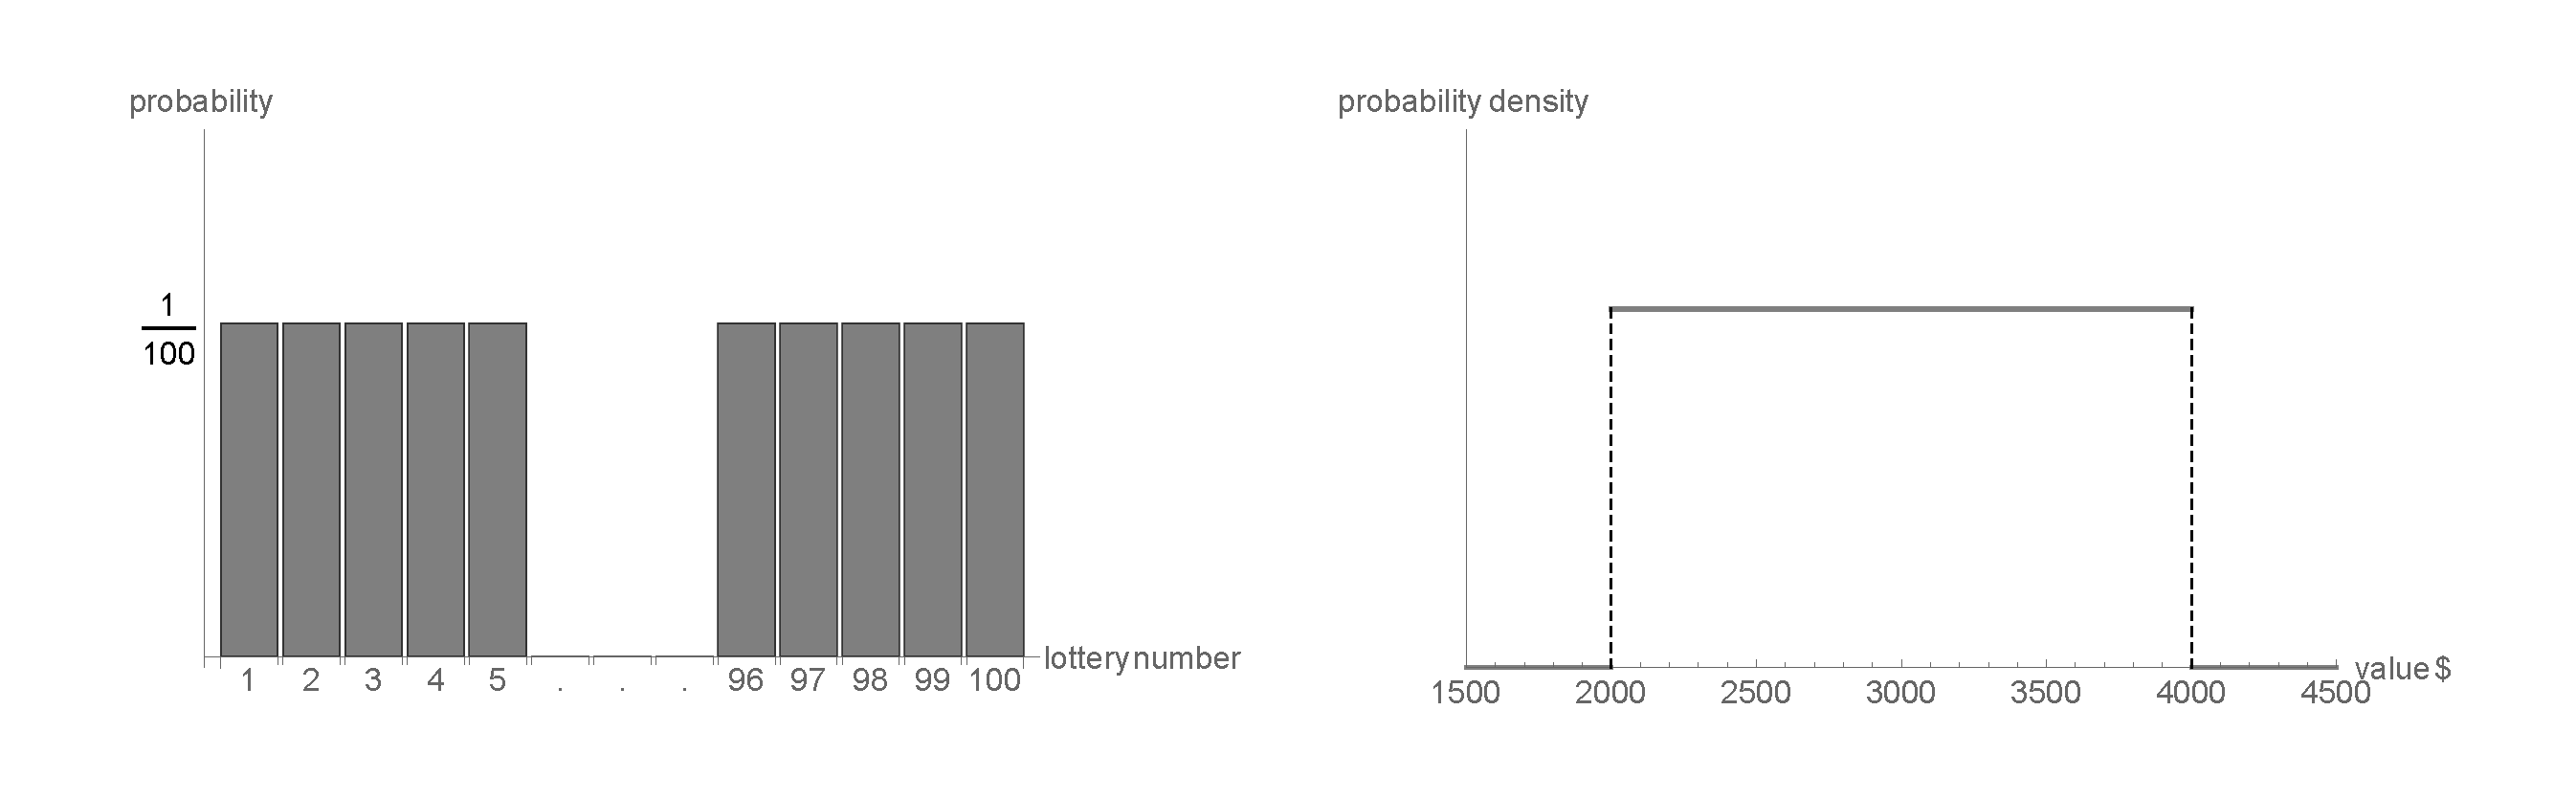
\includegraphics{Probability_lotterySecondhandCarProbability.pdf}}
\caption{Probability distributions representing \textbf{left:} the chance of winning a lottery, and \textbf{right:} the value of a second-hand car.}\label{fig:Probability_lotterySecondhandCarProbability}
\end{figure}

\subsection{What makes a probability distribution \textit{valid}?}\label{sec:Probability_validProbabilityDistribution}
The lottery example given in section \ref{sec:Probability_probabilityDistributions} refers to discrete probability distribution, since the variable we were measuring - the winning number - is confined to take on finite set of values. However, we could similarly define a probability distribution where our variable is able to take on an infinity of values across a spectrum. Imagine that before test drive a second-hand car we are uncertain about its value. We might think that from seeing pictures of the car, that it could be worth anywhere from \$2000 to \$4000, with all values being equally likely (see \ref{fig:Probability_lotterySecondhandCarProbability}).

The aforementioned examples are both examples of valid/proper probability distributions. So, what are their defining properties?

\begin{itemize}
\item All values of the distribution must be real, and non-negative.
\item The sum (integral) across all possible values of the discrete (continuous) random variable must be 1.
\end{itemize}

In the lottery case, this is satisfied since $p(X)=\frac{1}{100}\geq 0$, and:

\begin{equation}
\frac{1}{100} + \frac{1}{100} + ... + \frac{1}{100} = \sum\limits_{i=1}^{100} \frac{1}{100} = 1
\end{equation}

For the continuous case of the probability of a heads when flipping a coin, the probability distribution is always $\frac{1}{2000}\geq 0$, and when we do the continuous analogue of summing - integrating - we find that:

\begin{align}
\int\limits_{2000}^{4000} p(v) \mathrm{d}v &= \int\limits_{2000}^{4000} \frac{1}{2000} \mathrm{d}v\\
&= \left[\frac{1}{2000}v\right]^{4000}_{2000}\\
&= \frac{1}{2000}\left(4000-2000\right)\\
&= 1
\end{align}

Although, it may seem that this definition is relatively arbitrary, and perhaps well-trodden-territory for some readers, it is of \textit{central} importance to Bayesian statistics. This is because Bayesians like to work with, and produce \textit{valid} probability distributions. The pursuit of this ideal underlies the majority of \textit{all} methods in applied Bayesian statistics - analytic and computational - and hence its importance cannot be overstated!

\subsection{Probabilities vs probability density : interpreting discrete and continuous probability distributions}\label{sec:Probability_densityVsMassFunctions}
The discrete probability distribution for the lottery shown on the left hand side in figure \ref{fig:Probability_lotterySecondhandCarProbability}, is straightforward to interpret. To calculate the probability that the winning number, $X$, is 3, we simply read off the probability from the graph corresponding to the height of the leftmost bar, and find that:

\begin{equation}
p(X=3)= \frac{1}{100}
\end{equation}

In the discrete case, if we want to calculate the probability that a random variable takes on a range of values, then we simply need to sum the individual probabilities corresponding to each specific event. In the lottery example, if we want to calculate the probability that the winning number is 10 or less, we just add together the probabilities of it being \{1, 2, 3, 4, 5, 6, 7, 8, 9, 10\}:

\begin{align}
p(X\leq 10) &= p(X=1) + p(X=2) + p(X=3) + ... + p(X=9) + p(X=10)\\
&= \frac{1}{100} + \frac{1}{100} + \frac{1}{100} + ... + \frac{1}{100} + \frac{1}{100}\\
&= \frac{1}{10}
\end{align}

How can we use the continuous probability distribution such as the one shown on the right hand side of figure \ref{fig:Probability_lotterySecondhandCarProbability}? If we want to calculate the probability that the value of the second-hand car is \$2,500, then we could simply draw a vertical line from this point on the $value$ axis up to the line of the distribution; concluding that $p(value=\$2,500) = \frac{1}{2000}$! However, under this logic, we could also deduce that the probability of the value of the car being \{\$2,500,\$2,500.10,\$2,500.01,\$2,500.001\} are all $\frac{1}{2000}$. Furthermore, we could generate an infinity of these test values of $value$, meaning that if we summed them all together we could get a total probability of $\infty$. 

There is evidently something wrong with our method for interpreting continuous densities. If we reconsider the test values $\{\$2,500,\$2,500.10,\$2,500.01,\$2,500.001\}$, we reason that these are all equally unlikely, and part of a set of an infinity of potential values we could draw. This means for a continuous random variable, we always have $p(\theta=number) = 0$. Hence, when we write $p(\theta)$ for a continuous random variable, we should be careful to interpret the value of it at a particular value as a probability \textit{density}, \textit{not} a probability. 

However, we can use a continuous probability distribution to calculate the probability that a random variable lies between two bounds. To do this we use the continuous analogue of a sum, an \textit{integral}. For the car example, we can calculate, $\$2,500\leq \theta \leq \$3,000$:

\begin{align}\label{eq:Probability_continuousProbabilityIntervalExample}
Pr(2500\leq value \leq 3000) &= \int\limits_{2500}^{3000} p(v) \mathrm{d}v\\
&= \int\limits_{2500}^{3000} \frac{1}{2000} \mathrm{d}v\\
&= \left[\frac{1}{2000}v\right]_{2500}^{3000}\\ 
&= \frac{1}{2000}(3000-2500) = 0.25
\end{align}

In (\ref{eq:Probability_continuousProbabilityIntervalExample}), we have used $Pr$ to explicitly state that the result is a \textit{probability}, whereas $p(\theta)$ is a probability density. Of course, the calculation carried out in (\ref{eq:Probability_continuousProbabilityIntervalExample}), is equivalent to working out the area under the graph within those limits (see figure \ref{fig:Probability_continuousLotteryInterval}).

\begin{figure}
\centering
\scalebox{0.5} 
{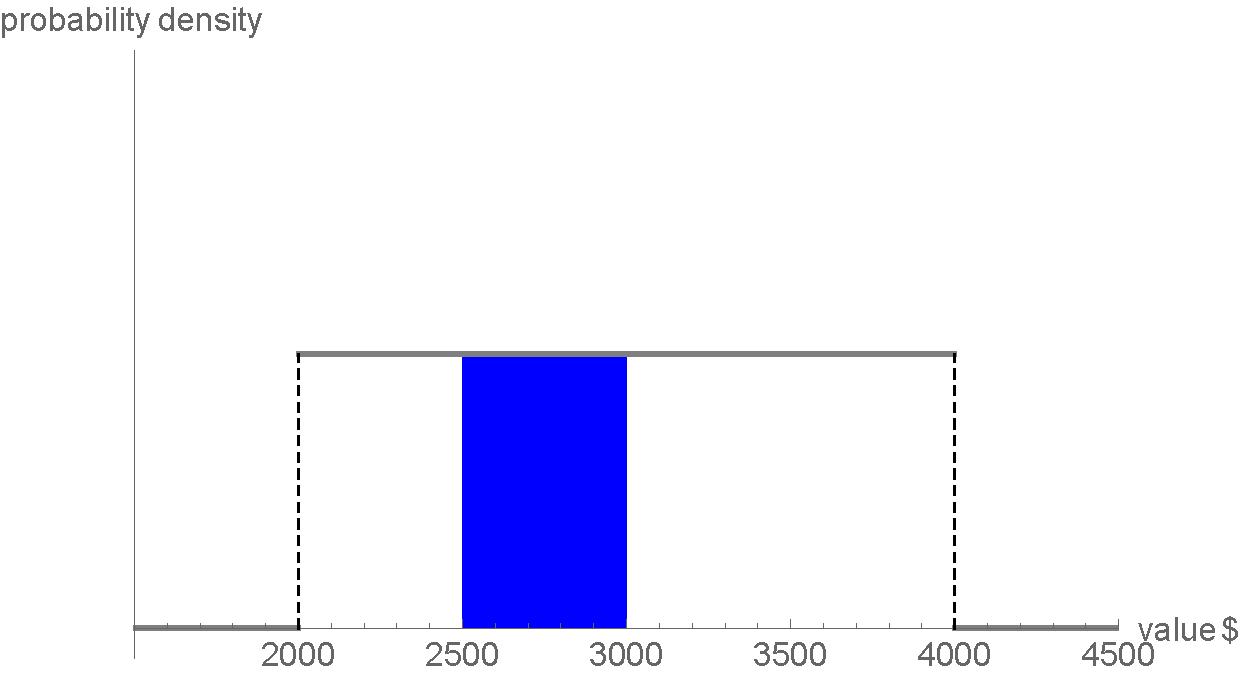
\includegraphics{Probability_continuousLotteryInterval.pdf}}
\caption{The probability that a second-hand car's value lies between \$2,500 and \$3,000.}\label{fig:Probability_continuousLotteryInterval}
\end{figure}

\boxed{Interactive:} see the interactive tool to allow you to dynamically manipulate figure \ref{fig:Probability_continuousLotteryInterval}.

A quick note on terminology: often theorists use probability \textit{mass} to handle discrete distributions, where the distribution's values are directly interpretable as probabilities, and probability \textit{densities} to handle continuous distributions. The latter need to be integrated to yield a probability. We eschew the 'mass' terminology as we find it counter-productive to differentiate between the two types of distributions, since Bayes' rule handles them in the same way (see below).

\boxed{Video:} see the video XXX which explains more about the difference between a probability and a probability density. A coin hidden in a Christmas pudding would be a good example.

\subsubsection{A (wet) river crossing}
Imagine you wish to cross a fast-flowing river to reach friends on the other side. Unbeknownst to you, a rather devious park ranger has arranged 6 stepping stones which \textit{guarantee} a person attempting to cross the river will suffer a wet fate! Since you are guaranteed a damp walk home, the only uncertainty is exactly \textit{where} along the stepping stone route you will fall. Your friends/schadenfreunde are anticipating this outcome, and have assigned probabilities of you falling when attempting to reach each individual stone; the higher the stone, the more probable a person will fall into the water whilst trying to reach it (see figure \ref{fig:Probability_riverCrossing}). In this case, there only 6 outcomes to the crossing: you fall from stone 1, 2, 3, 4, 5, or 6 (we suppose that if a person did manage to get to the last stone, they would always reach the opposite bank). Thus each of these \textit{discrete} outcomes is associated with its own non-zero probability. 

By contrast imagine that the malevolent omnipotent ranger has instead arranged a bridge across the river; again through their powers they have ensured that you will \textit{definitely} fall whilst attempting to navigate the path. Again your friends want to try to make sense of this divine intervention, and want to assign probabilities to each of the outcomes. However, this is different to before, since there are no longer a finite number of possible places where you can fall; there are in fact, a infinite continuum of possibilities. Here you could fall from a point 5m from the bank, or 5.000001m from the bank! Clearly here we are not going to be able to assign a positive probability to all of these possible outcomes, since this would result in the total probability integrating to infinity. Instead of attempting this full-hardy task, your friends instead prefer to deal with probabilities across particular non-zero intervals of the bridge length, again deciding that the higher the bridge, the greater the probability of you falling (see the middle panel of figure \ref{fig:Probability_riverCrossing}). Thus here in order to get out the quantity of interest - a probability of falling across a small interval - we are required to multiply our measure - now called a probability \textit{density} - by the small length of bridge interval over which we are concerned. Note we have used a small interval here so that we can assume that the measure is unchanging across its length. Also notice that a probability density has no meaning without a corresponding length scale; in this case we can think of the density of having `units' probability/meter.  

Finally imagine that it is winter, and now the very top the river is frozen, allowing you the possibility of choosing your own (potentially) non-straight-line path across. Again we invoke the idea of our cunning (increasingly-deified) ranger who has determined that you will fall at some point in your attempted crossing. Your friends now note that the ice is thicker in some places than others, and hence the potentiality of falling in some places is greater than others. We suppose that we can characterise a given point in the path by its distance across the river - the y direction - together with the transverse distance along the bank - called `x'. This allows your friends to construct a probability density which is now defined in terms of these two coordinates. Again we see immediately that there are an infinity of different possible places where you could fall, for example, at a point (1.1m, 3.2m) or (1.1000001m,3.2000000001m) across. Clearly now in order for our density must have `units' probability/$m^{-2}$. Thus to calculate the quantity of interest - a probability of falling across a small area - we are required to multiply the value of the probability density by the corresponding value of area. 

In closing our discussion of the differences between probabilities and probability densities, we note that in the case of the latter we always need to supply a `volume' which provides the necessary exchange rate for converting to a probability. Note the word `volume' is used for its analogy with 3D solids, where we can calculate the mass of an object by multiplying the density by the volume. Analogously here we can calculate the \textit{probability mass} of an infinitesimal volume:
%
\begin{equation}
probability\; mass = probability\; density \times volume
\end{equation}
%
However, here a volume need not correspond to an actual 3D volume in space, but corresponds to a unit of measurement across the range of a random variable of interest. In the above examples we first used a length, then an area as our volume unit, however in other examples it could correspond to a weight, percentage or even a probability.

\begin{figure}
\centering
\scalebox{0.2} 
{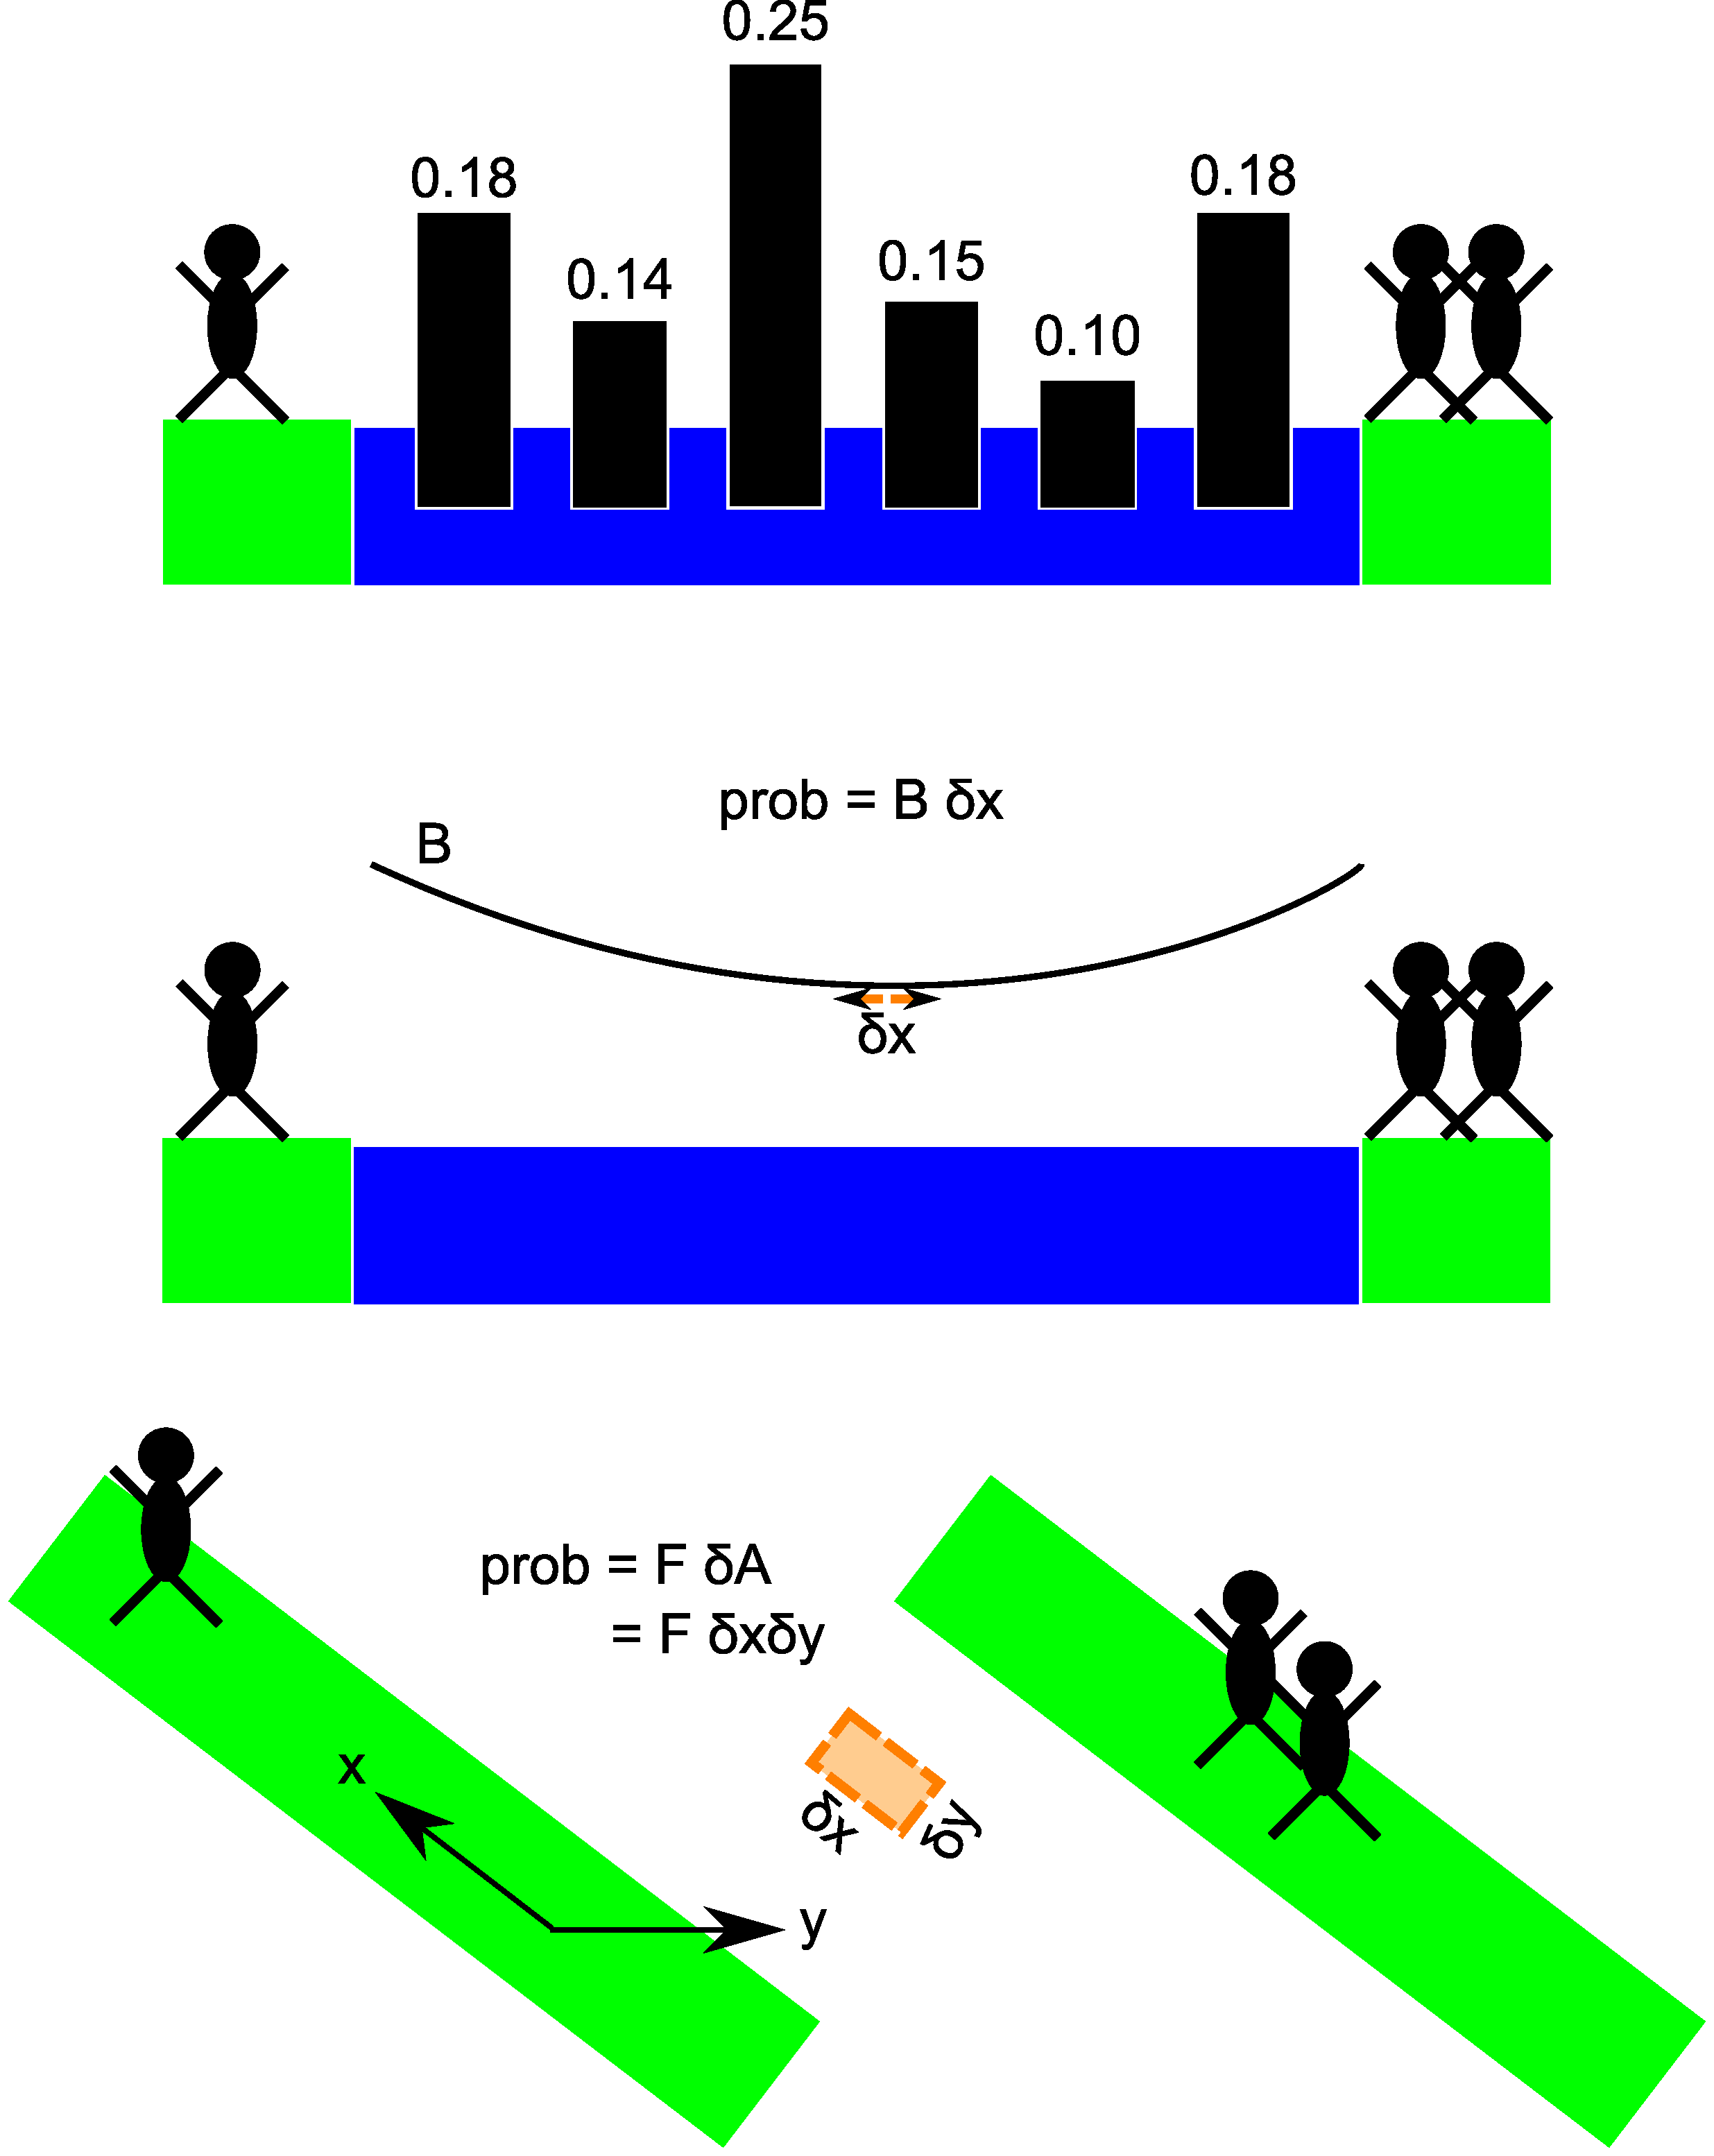
\includegraphics{Probability_riverCrossing.pdf}}
\caption{Top: crossing on discrete stepping stones. Middle: crossing via a bridge whose height (B) is a probability density. Bottom: crossing on thin ice - the thickness of the ice (F) represents a probability density.}\label{fig:Probability_riverCrossing}
\end{figure}

\subsubsection{Probability zero vs impossibility}
You may be left wondering, if we have a continuous distribution over some interval - say a standard normal distribution which could potentially output any real number from minus infinity and plus infinity - then the aforementioned discussion of probabilities vs probability densities suggests that the probability of exactly obtaining any particular number is zero. However, does this mean that it is impossible to obtain a particular number? If you answered `yes' here, then how can we ever hope to obtain a sample of numbers from our distribution, since they are all individually impossible? The apparent paradox at hand is subtle, but important nonetheless. Whilst a full explanation of this issue requires a knowledge of \textit{measure theory}, we can still attempt a more heuristic explanation.

When we say an event is impossible, we always say that it has a probability zero. Essentially when we use the word `impossible' we are saying that the event does not appear within our space of potential eventualities. Imagine the event that you simultaneously conclude \textit{both} of the following about a ball withdrawn from an urn of many balls:

\begin{itemize}
\item The ball is entirely white.
\item The ball is entirely black.
\end{itemize} 

Philosophically, we could argue that such an event is impossible. We shouldn't even include it in our set of possible outcomes. Thus this event corresponds to an empty set in our outcome space. The empty set by default is assigned a probability zero, meaning that the above white/black ball outcome is also assigned a probability of zero.

Alternatively, going back to our example of a sample of numbers from a standard normal, we would assign the purely imaginary number $i$, to the empty set since it lies outside of the range of such a distribution; meaning it is impossible. By converse, consider attempting to exactly guess the number that we obtain from our distribution. Clearly obtaining the number 3.142 here \textit{is} possible - it does not lie outside of the range of the distribution - so we shouldn't assign it to the empty set. However, if we multiply our probability density by the volume corresponding to this particular value, then we get zero, because the volume element is of zero width! So we see that events that have probability zero, \textit{can} still be possible. 

So basically, we have learned that events that are impossible have zero probability. However, the converse is \textit{not} true: events that are of zero probability are still possible. If this still does not sit right with you, then remember that probabilities are just units of measurement. For a Bayesian they measure subject points of view, so clearly an event to which we assign zero probability can still happen. For a Frequentist, they measure the outcome of an infinite series of identical trials. In our distribution example we can imagine attempting to guess the number our distribution outputs for each sample. We could then enumerate the ratio: $\frac{\#successes}{\#trials}$. Whilst we might correctly guess the number a few times, clearly the denominator here would dominate (go to infinity), and we would still get a probability of zero.

\subsubsection{The good news: Bayes' rule doesn't distinguish between probabilities and probability densities}
Whilst it is important to understand that probabilities and probability densities are \textit{not} the same type of entity, the good news for us is that Bayes' rule is the same for each. So we can readily write:

\begin{equation}
Pr(\theta=1|X=1) = \frac{Pr(X=1|\theta=1)Pr(\theta=1)}{Pr(X=1)}
\end{equation}

for the case of when the data, $X$, and the parameter $\theta$ are discrete, and hence $Pr$ denotes a probability.

Alternatively, we can write Bayes' rule as:

\begin{equation}
p(\theta=1|X=1) = \frac{p(X=1|\theta=1)p(\theta=1)}{p(X=1)}
\end{equation}

for the case when the data and parameter are continuous, and $p$ denotes a probability density.

We will more commonly use the latter representation since for the majority of cases, the parameters will be continuous.

\subsection{Mean and variance of distributions}\label{sec:Probability_meanVariance}
A popular way of summarising a distribution is via its \textit{mean}, which is one measure of central tendency of a distribution. More intuitively, a mean, or \textit{expected value}, of a distribution represents the long-run average value that would be obtained if we sampled from that particular distribution in question, an infinite number of times. 

The way in which we calculate the \textit{mean} of a distribution depends on whether it is \textit{discrete} or \textit{continuous} in nature. However, the concept is essentially the same in both cases. The mean is calculated as a weighted sum of the values taken on by the random variable in question, where the weights are provided by the probability distribution. This results in the following forms for the mean of a discrete and continuous variable respectively:

\begin{equation}\label{eq:Probability_meanDistributionDiscrete}
\mathbb{E}(X) = \sum\limits_{All\; \alpha} \alpha Pr(X=\alpha)
\end{equation}

\begin{equation}\label{eq:Probability_meanDistributionContinuous}
\mathbb{E}(X) = \int\limits_{All\; \alpha} \alpha p(\alpha)\mathrm{d}\alpha
\end{equation}

In (\ref{eq:Probability_meanDistributionDiscrete}) and (\ref{eq:Probability_meanDistributionContinuous}), $\alpha$ represents the multitude, or continuum of \textit{values} taken on by the random variable $X$ respectively.  We have chosen to use $Pr$ in (\ref{eq:Probability_meanDistributionDiscrete}), and $p$ in (\ref{eq:Probability_meanDistributionContinuous}), to illustrate that these represent probabilities and probability \textit{densities} respectively.

We can now apply (\ref{eq:Probability_meanDistributionDiscrete}) to allow us to calculate the mean winning number from the lottery:

\begin{align}\label{eq:Probability_meanLottery}
\mathbb{E}(X) &= \sum\limits_{\alpha=1}^{100} \alpha Pr(X=\alpha)\\
&= 1\times\frac{1}{100} +  2\times\frac{1}{100} +  3\times\frac{1}{100} + ... +  99\times\frac{1}{100} +  100\times\frac{1}{100}\\
&= 50\tfrac{1}{2}
\end{align}

We can also demonstrate the \textit{long-run} nature of the mean value of $50\tfrac{1}{2}$ found in (\ref{eq:Probability_meanLottery}) by simulating a number of rolls of a fair die computationally (see figure \ref{fig:Probability_meanDiscreteLongRun}). As the number of rolls increases, the running mean tends towards this value.

\begin{figure}
\centering
\scalebox{0.55} 
{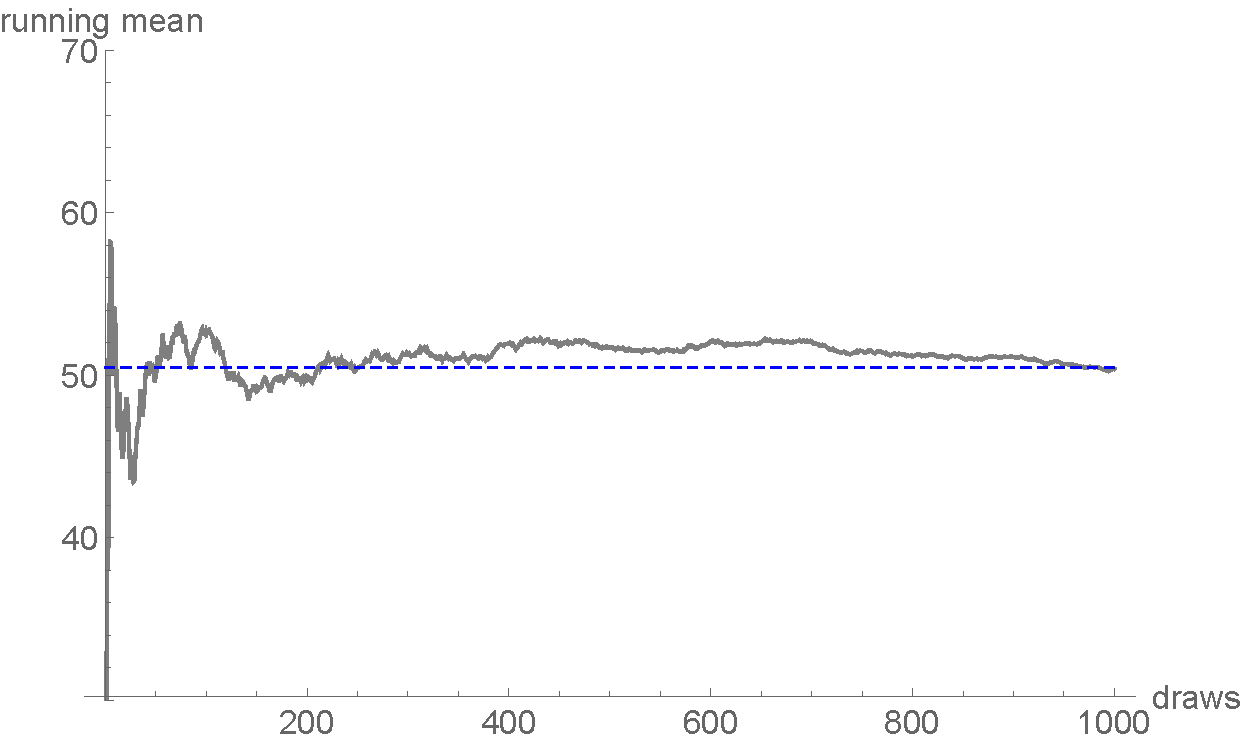
\includegraphics{Probability_meanDiscreteLongRun.pdf}}
\caption{Playing a computational lottery. We see the approach of the running mean of repeatedly playing the lottery to the long-run mean of $50\tfrac{1}{2}$, as the number of plays increases.}\label{fig:Probability_meanDiscreteLongRun}
\end{figure}

We can also apply (\ref{eq:Probability_meanDistributionContinuous}) to calculate our expectation of the second-hand car value:

\begin{align}\label{eq:Probability_meanCoinContinuous}
\mathbb{E}(value) &= \int\limits_{2000}^{4000} v p(v)\mathrm{d}v\\
&=\frac{1}{2000} \int\limits_{2000}^{4000} v \mathrm{d}v\\
&= \frac{1}{2000}\left[\frac{v^2}{2}\right]^{4000}_{2000}\\ 
&= \$3,000
\end{align}

If we were to have a business buying (and selling) second-hand cars, we might keep tabs on the values of cars we buy over time. If all cars came from the same uniform distribution that we have proposed, then we would see the sample average value approaching the above long-run mean of \$3,000, as the number of cars we buy gets large\footnote{Technically, tends to infinity.} (see figure \ref{fig:Probability_meanContinuousLongRun}).

\begin{figure}
\centering
\scalebox{0.55} 
{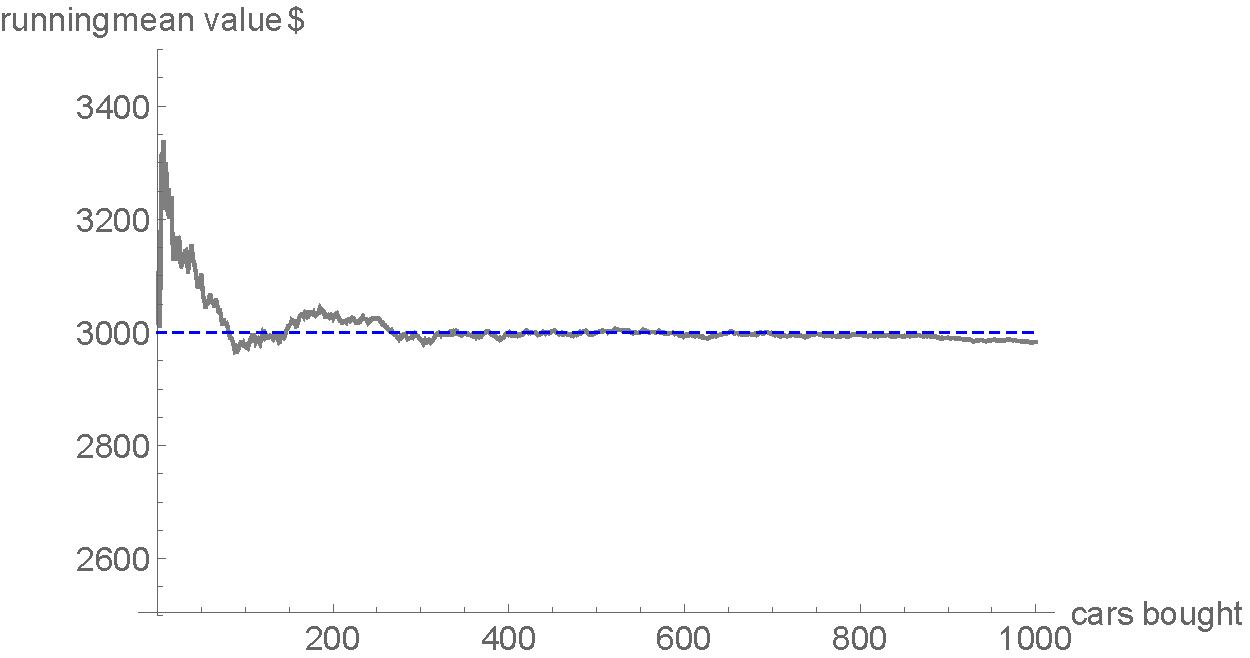
\includegraphics{Probability_meanContinuousLongRun.pdf}}
\caption{Career second-hand car sales. We can see the approach of the sample mean towards the long-run mean of \$3,000.}\label{fig:Probability_meanContinuousLongRun}
\end{figure}

If you can grasp the process undertaken to produce figures \ref{fig:Probability_meanDiscreteLongRun} and \ref{fig:Probability_meanContinuousLongRun} respectively, then you already understand the basis behind modern computational Bayesian statistics! If you need a bit more explanation of the theory of Bayesian computational, then fear not, we devote an entire Part of the book for this purpose (see Part \ref{part:computationalBayes}).  

Whilst the \textit{mean} of a distribution is a measure of central tendency for a particular distribution, we do not yet have a way of summarising the width of the range of the values of the random variable which are most likely. This motivates the introduction of the concept of a \textit{variance} of a distribution:

\begin{equation}\label{eq:Probability_varianceDistributionExpectations}
var(X) = \mathbb{E}\left(\left[X-\mathbb{E}(X)\right]^2\right)
\end{equation}

To apply (\ref{eq:Probability_varianceDistributionExpectations}) to discrete and continuous distributions respectively, we straightforwardly replace the $\alpha$ on the right-hand side of (\ref{eq:Probability_meanDistributionDiscrete}) and (\ref{eq:Probability_meanDistributionContinuous}) respectively, by $(\alpha-\mathbb{E}(X))^2$ in each case\footnote{This is a specific example of the general rule, that to calculate the mean value of some function $f(X)$, where $X$ is governed by a particular distribution, we do: \begin{equation}
\mathbb{E}(f(X)) = \sum\limits_{All\; \alpha} f(\alpha) Pr(X=\alpha)
\end{equation}
for a discrete distribution, and analogously for the continuous case, but using an integral opposed to a sum.}:

\begin{equation}\label{eq:Probability_varianceDistributionDiscrete}
var(X) = \sum\limits_{All\; \alpha} (\alpha-\mathbb{E}(X))^2 Pr(X=\alpha)
\end{equation}

\begin{equation}\label{eq:Probability_varianceDistributionContinuous}
var(X) = \int\limits_{All\; \alpha} (\alpha-\mathbb{E}(X))^2 p(\alpha)\mathrm{d}\alpha
\end{equation}

If the equations are starting to overwhelm, then fret not, we really only wanted to include them for completeness. What is more important is their significance. Essentially, a \textit{variance} measures the width of the distribution of values obtained around its mean. A wider variance therefore signifies a greater variety of values away from the mean. In figure \ref{fig:Probability_varianceLottery} we compare the variability of the fair lottery, with one heavily biased to take on the values between 40 and 60. We see that the variability of the running mean for the biased lottery is smaller than that of the fair one, particularly as the number of rolls increases. This is due to the fact that the fair lottery has a variance of:

\begin{align}
var(X) &= \sum\limits_{\alpha=1}^{100} (\alpha-50\tfrac{1}{2})^2\times Pr(X=\alpha)\\
&= 833\tfrac{1}{4}
\end{align}

whereas similar calculations for the loaded die distribution shown in the middle of figure \ref{fig:Probability_varianceLottery}, yield a value of approximately 265. To be concrete, the variance of a distribution is an indicator of the long-run average square distance of values away from the mean. 

\begin{figure}
\centering
\scalebox{0.35} 
{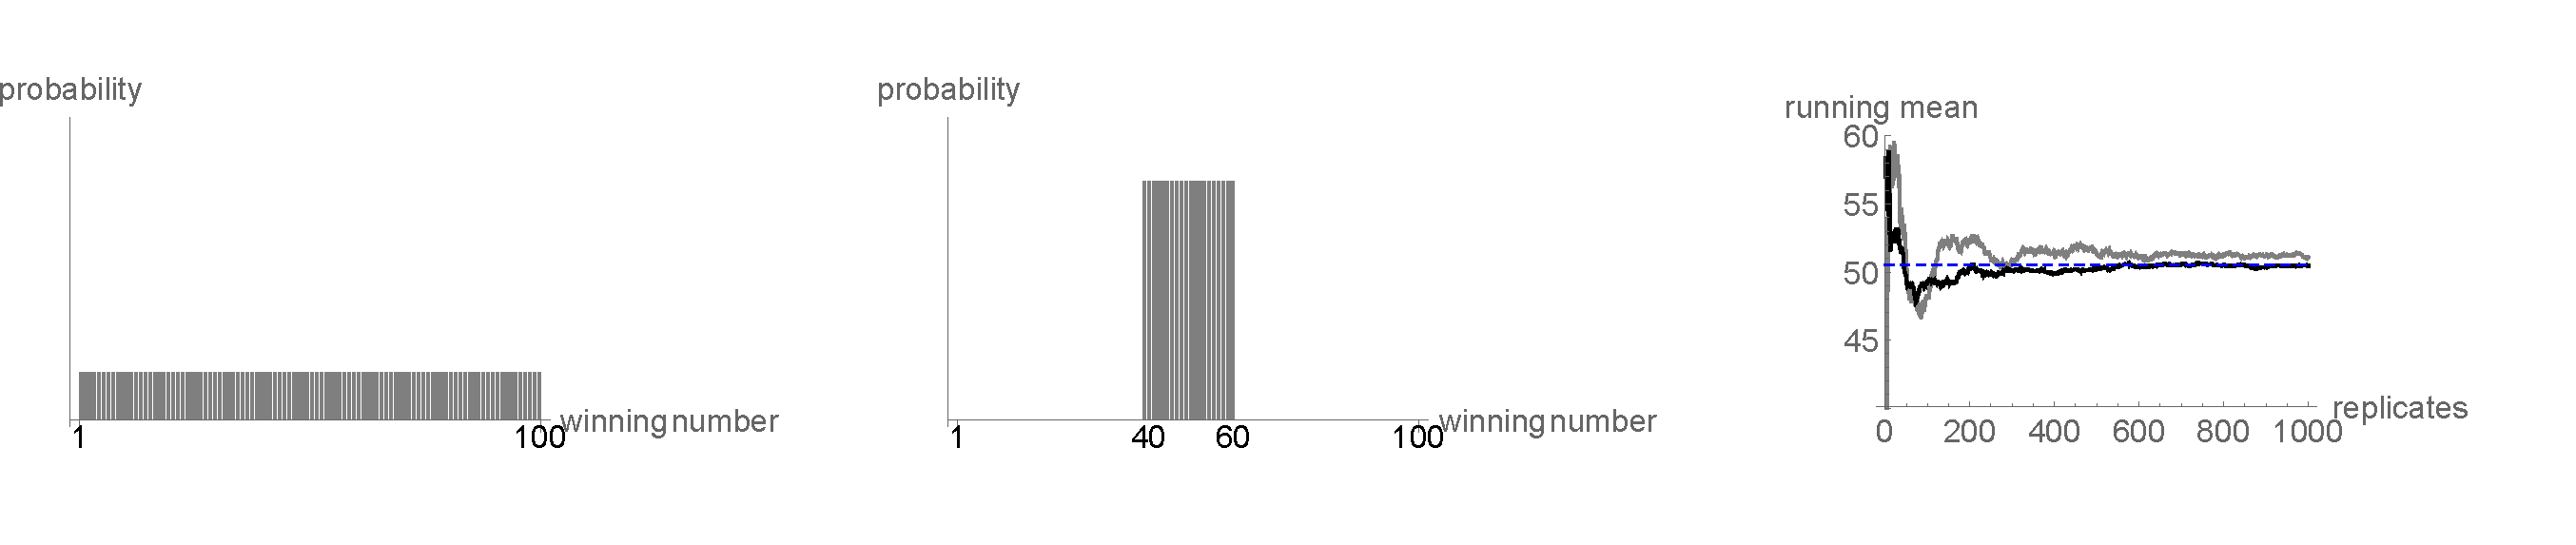
\includegraphics{Probability_varianceLottery.pdf}}
\caption{Comparing the variance of two lotteries, left: a lottery where all values between 0 and 100 are equally likely. Middle: a lottery where only values between 40 and 60 have a positive probability. Right: comparing the variability of these distributions about their common mean.}\label{fig:Probability_varianceLottery}
\end{figure} 

\subsection{Generalising probability distributions to two dimensions}
Life is often more complex than the examples of section \ref{sec:Probability_probabilityDistributions}. Often we are tasked with formulating opinions on a range of different outcomes; each of which may influence or shed light on the other results. We begin by considering the outcome of two measurements, in order to introduce the reader to the mechanics of probability. The great thing is that these rules do not become any more complex when we generalise to higher dimensional problems, meaning that if the reader is comfortable with the following examples, then they should be able to handle the vast majority of probability distribution operations encountered. In Bayesian statistics, being comfortable manipulating probability distributions is essential, since the output of the Bayesian formula - the posterior probability distribution - is used to derive all post-experiment conclusions. As such, it is important to devote some time to introduce two examples which we will use to describe and explain the manipulations of 2-dimensional probability distributions.

\subsubsection{Horses for courses: a 2-dimensional discrete probability example}\label{sec:Probability_biasedCoinsTwoDimensionalDiscrete}
Imagine that you are a horse racing aficionado, and are interested in quantifying the uncertainty regarding the outcome of two (fictitious) races for two thoroughbreds in a particular stable. From their historical performance over 100 races you notice that both horses tend to react in the same way to the racing conditions. When horse A wins, it is more likely that, later in the day, horse B will win, and vice versa. Similarly regarding the losses; when horse A finds the going tough, so does horse B. Wanting to flex your statistical muscle, you choose to represent this information by the two-dimensional probability distribution shown in table \ref{tab:Probability_coinBiased}

\begin{table}[htbp]
  \centering
    \begin{tabular}{rrcc}
    \toprule
          &       & \multicolumn{2}{c}{\textbf{horse A}} \\
    \midrule
          &       & \textbf{0} & \textbf{1} \\
    \multicolumn{1}{c}{\textbf{horse B}} & \multicolumn{1}{c}{\textbf{0}} & $\frac{30}{100}$   & $\frac{10}{100}$ \\
    \multicolumn{1}{c}{} & \multicolumn{1}{c}{\textbf{1}} & $\frac{10}{100}$   & $\frac{50}{100}$ \\
    \bottomrule
    \end{tabular}%
  \caption{A probability distribution showing the historical performance of two horses, A and B, in two separate races. $\{0,1\}$ refers to each horse losing or winning in their respective races.}\label{tab:Probability_coinBiased}
\end{table}

How can we check whether this distribution satisfies the requirements for a valid probability distribution? We simply apply the rules described in section \ref{sec:Probability_validProbabilityDistribution}. Firstly, all the values of the distribution are real and non-negative; satisfying our first requirement. For the second rule rather than summing over the values of one random variable, we now have to sum over the outcome of two:

\begin{equation}\label{eq:Probability_discreteTwoDimensionalCoinSum}
\sum\limits_{X_A=0}^{1}\sum\limits_{X_B=0}^{1} Pr(X_A,X_B) = \frac{30}{100} + \frac{10}{100}  + \frac{10}{100}  + \frac{50}{100}  = 1
\end{equation}

In (\ref{eq:Probability_discreteTwoDimensionalCoinSum}), $X_A$ and $X_B$ are random variables\footnote{A function which associates a unique numerical value with each outcome of an experiment. In this case the function gives value 0 if the result is a tails, and 1 if it is heads.} which refer to the outcome of the races for horse A and horse B respectively. Notice that since we are now considering a situation with the outcome of two random variables, we are now required to index the probability, $Pr(X_A,X_B)$, by both. Due to the probability now being a function of two variables, we say that the probability distribution is 2-dimensional.

How can we interpret the probability distribution shown in table \ref{tab:Probability_coinBiased}? The probability that both horses lose (and hence both their random variables take on the value of 0), is simply read off from the top-left entry in the table, meaning $Pr(X_A=0,X_B=0)=\frac{30}{100}$. We ascribe a smaller likelihood to heterogeneous outcomes, $Pr(X_A=0,X_B=1)=\frac{10}{100}$ or $Pr(X_A=1,X_B=0)=\frac{10}{100}$, since we believe that the horses are more likely to react similarly to the racing conditions. We believe that the most likely outcome is that both horses win, since historically the horses have done well on this particular racing course, and hence ascribe the highest probability to this result, with $Pr(X_A,X_B)=\frac{50}{100}$.

\subsubsection{Foot length and literacy: a 2-dimensional continuous probability example}
We suppose that we have a sample of individuals, and we measure their foot size, as well as how well they score on a literacy test. Both of these variables can reasonably be assumed to be continuous, meaning that we are now required to represent our strength of belief, by specifying a probability distribution across a continuum of values (see figure \ref{fig:Probability_footSizeIntelligenceTwoDimensionalExample}). 

%\begin{figure}
%\centering
%\scalebox{0.5} 
%%{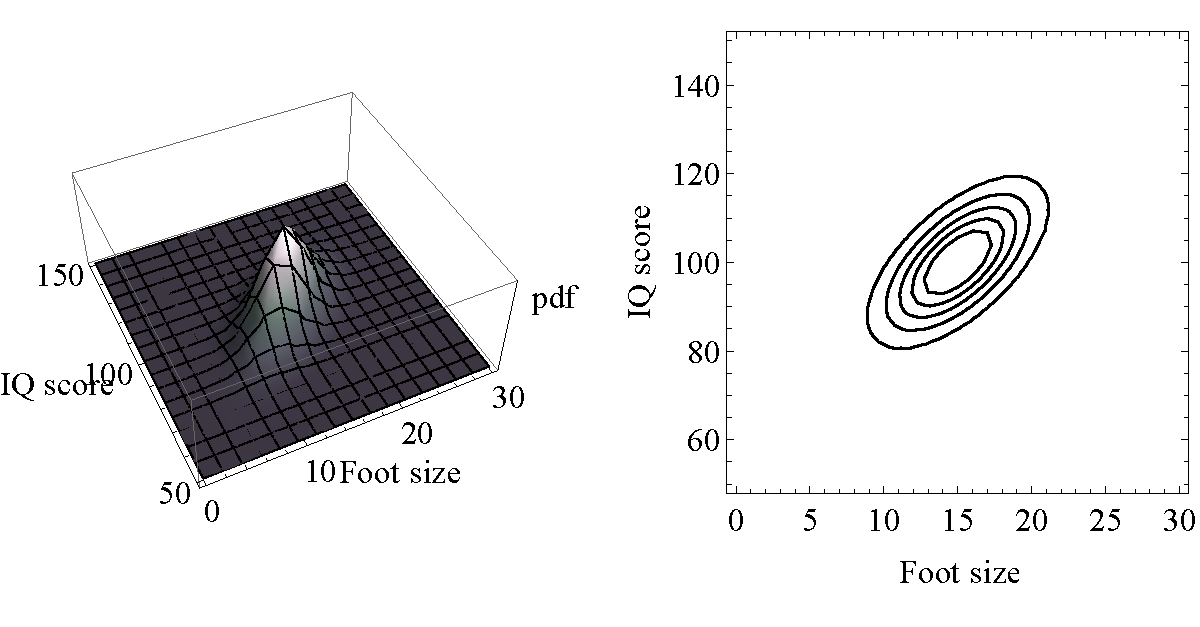
\includegraphics{Probability_footSizeIntelligenceTwoDimensionalExample.pdf}}
%\caption{A probability distribution describing the foot size and scores on a literacy test for an individual within our sample. Left) Represented as a 3-dimensional plot, and Right) Contour lines specify isolines of probability.\textbf{Left out figure as it was too big, and was causing latex to crash!}}\label{fig:Probability_footSizeIntelligenceTwoDimensionalExample}
%\end{figure}

We could verify that the distribution shown in figure \ref{fig:Probability_footSizeIntelligenceTwoDimensionalExample} is in fact valid, by showing that the volume underneath the left hand plot is 1, via integration. However, since we don't want to overcomplicate things now, you will have to take our word for it.

Notice that there to be a degree of correlation between foot size and scores on the literacy test. Why might this be the case\footnote{Our sample of individuals here is a sample of children of various ages. Age is correlated with shoe size and literacy.}?

\subsection{Marginal distributions}\label{sec:Probability_marginal}
We may be interested in simplifying the preceding analysis, by stating the distribution of one variable, completely \textit{unconditional} of the other. In our horses example, we might be interested in say, only the result of the first horse race, which involves horse A. Alternatively, we might want to remove the dependence on foot size, in our literacy score example, and what remains would then be an \textit{unconditional} probability distribution for literacy score.

In order to do this, we essentially need to \textit{average} out the dependence of the other variable. In our horses example, if we are only interested in the result of horse A, we can sum down the column values for horse B, obtaining the \textit{marginal} distribution of horse A, shown at the bottom of table \ref{tab:Probability_coinsMarginal}.


\begin{table}[htbp]
  \centering
    \begin{tabular}{rrccr}
    \toprule
          &       & \multicolumn{2}{c}{\textbf{horse A}} &  \\
    \midrule
          &       & \textbf{0} & \textbf{1} & \multicolumn{1}{c}{\textbf{$Pr(X_B)$}} \\
    \multicolumn{1}{c}{\textbf{horse B}} & \multicolumn{1}{c}{\textbf{0}} & $\frac{30}{100}$   & $\frac{10}{100}$    & \multicolumn{1}{c}{\textbf{$\frac{40}{100}$ }} \\
    \multicolumn{1}{c}{} & \multicolumn{1}{c}{\textbf{1}} & $\frac{10}{100}$    & $\frac{50}{100}$    & \multicolumn{1}{c}{\textbf{$\frac{60}{100}$ }} \\
          & \multicolumn{1}{c}{\textbf{$Pr(X_A)$}} & \textbf{$\frac{40}{100}$ } & \textbf{$\frac{60}{100}$ } & \multicolumn{1}{c}{} \\
    \bottomrule
    \end{tabular}%
  \caption{The marginal distribution of horses A and B, achieved by summing the values in each column or row respectively.}\label{tab:Probability_coinsMarginal}%
\end{table}%

Hence, we have that the \textit{marginal} probability of horse A winning is 0.6. This value is composed out of the two possible ways in which this \textit{single} event can occur:

\begin{equation}\label{eq:Probability_marginalCoinsExample}
Pr(X_A=1) = Pr(X_A=1,X_B=0) + Pr(X_A=1,X_B=1)
\end{equation}

In (\ref{eq:Probability_marginalCoinsExample}), we see that A can win with B losing, or alternatively both horses can win.

Thus, in order to calculate the probability of a single event, we simply need to sum across all possible occurrences of it, allowing the other variable to take on its possible values. Mathematically, we can summarise this rule by the following for the case of two discrete random variables:

\begin{equation}\label{eq:Probability_marginalDiscreteProbabilityTwoDimensions}
Pr(A=\alpha) = \sum\limits_{\beta} Pr(A=\alpha,B=\beta)
\end{equation}

In (\ref{eq:Probability_marginalDiscreteProbabilityTwoDimensions}), $\alpha$ and $\beta$ refer to the specific values taken on by the random variables $A$ and $B$. 

We can use (\ref{eq:Probability_marginalDiscreteProbabilityTwoDimensions}) for the horses example to calculate the probability that horse B loses:

\begin{align}
Pr(X_B=0) &= \sum\limits_{\alpha=0}^{1} Pr(X_B=0,X_A=\alpha)\\
&= Pr(X_B=0,X_A=0) + Pr(X_B=0,X_A=1)\\
&= \frac{30}{100}  + \frac{10}{100}  = \frac{40}{100} 
\end{align}

For continuous random variables we need the continuous analogue of a sum, an \textit{integral}, in order to calculate the marginal distribution. Intuitively, this is because the other variable is now able to take on an continuum of values:

\begin{equation}\label{eq:Probability_marginalContinuousProbabilityTwoDimensions}
p_A(\alpha) = \int\limits_{All\;\beta} p_{AB}(\alpha,\beta) \mathrm{d}\beta
\end{equation}

In (\ref{eq:Probability_marginalContinuousProbabilityTwoDimensions}), $p_{AB}(\alpha,\beta)$ corresponds to the joint probability distribution of random variables $A$ and $B$ evaluated at $(A=\alpha,B=\beta)$. Similarly, $p_A(\alpha)$ refers to the marginal distribution of random variable A, evaluated at $A=\alpha$. Although it is somewhat of an abuse of notation, for simplicity, from now on we will now write $p_{AB}(\alpha,\beta)$ as $p(A,B)$, and $p_A(\alpha)$ as $p(A)$.

In the foot size/literacy example, we may not be interested in foot size; wanting only the distribution of literacy scores in our sample. We can obtain this by simply integrating out the dependence on foot size:

\begin{equation}\label{eq:Probability_marginalContinuousProbabilityTwoDimensionsFootExample}
p(score) = \int\limits_{0}^{30} p(score,FS) \mathrm{d}FS
\end{equation}

The result of carrying out the step in (\ref{eq:Probability_marginalContinuousProbabilityTwoDimensionsFootExample}) is that we are left with the distribution shown on the right of figure \ref{fig:Probability_footSizeIntelligenceMarginal}. We have rotated this graph to emphasise that it is the result of essentially summing\footnote{We really mean integrating, but it is more intuitive to think about this in terms of discrete summing.} across the joint density at each particular value of literacy scores. 

Another way to think about marginal densities, is imagine that you are walking along the landscape of the joint density. The total distance walked - horizontally and vertically - from $FS=0$ to $FS=30$ along a line of constant literacy, gives the height of the marginal density for literacy score at that point. If the path is relatively flat, indicating a low value of joint density, then the corresponding marginal density is low. However, if the path encompasses a large hill, indicating a high value of joint density, then the marginal density will be relatively high.

Add a 3D version of the figure with the contours traced out on the landscape, and leading to the height of the marginals, perhaps with stick figures walking along lines of iso-literacy.

\begin{figure}
\centering
\scalebox{0.5} 
{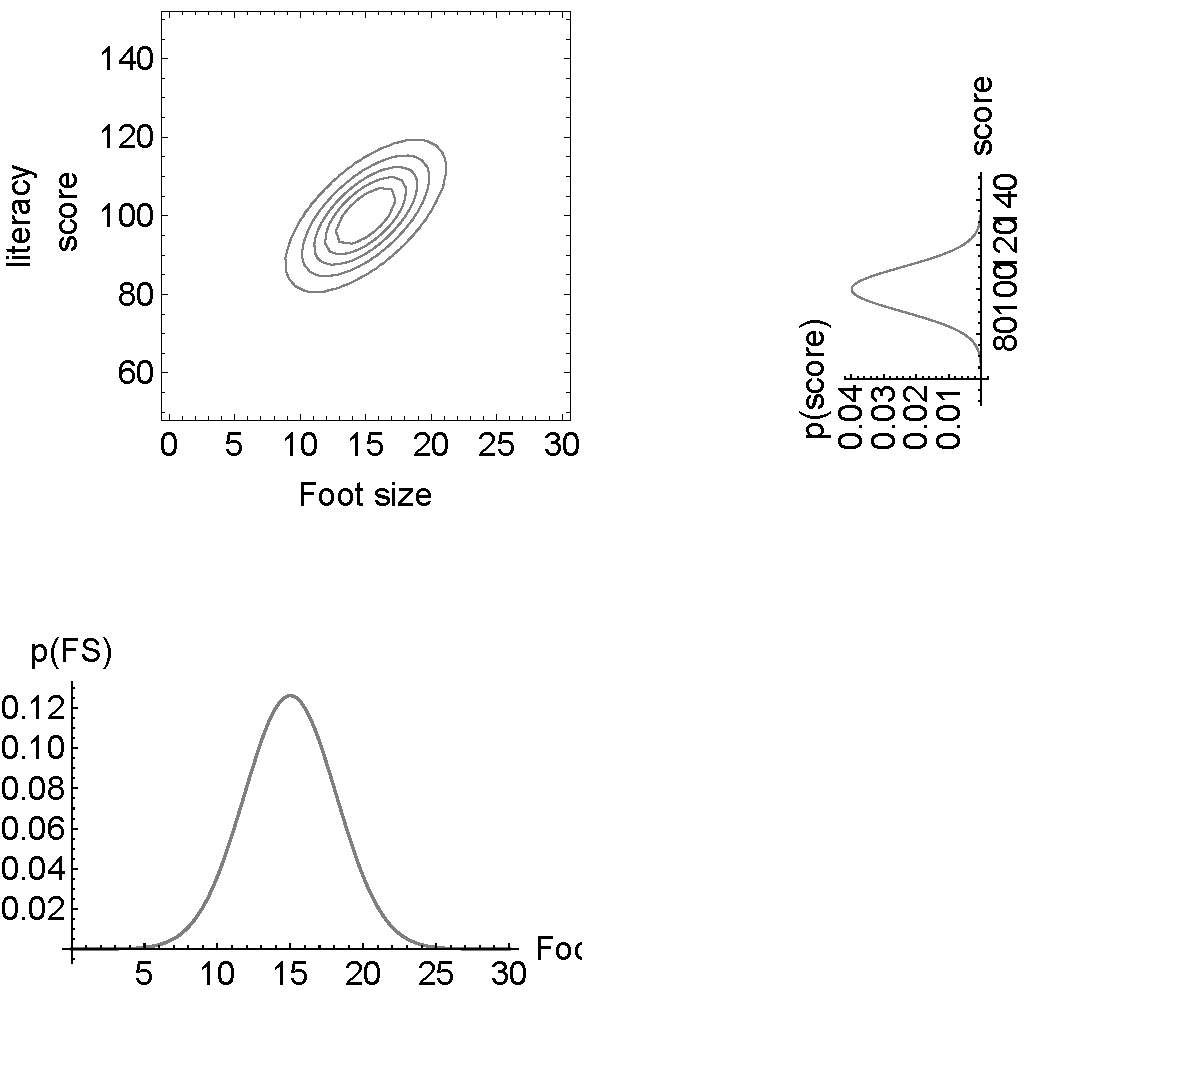
\includegraphics{Probability_footSizeIntelligenceMarginal.pdf}}
\caption{Top-left: the joint density of foot size and intelligence. Right: the marginal density of literacy scores. Bottom: the marginal density of foot size. \textbf{I want to add a line at a particular value of literacy scores, and at a particular value of FS, to illustrate the horizontal and vertical summing.}}\label{fig:Probability_footSizeIntelligenceMarginal}
\end{figure}

\subsubsection{Venn diagrams}
An alternative way of thinking about marginal distributions is provided by the Venn diagram shown in figure \ref{fig:Probability_Venn}. In a Venn diagram, the area of a particular event indicates its probability, and the rectangular area represents all the events that can possibly happen, and so has an area of 1. We have chosen to specify the events of horse A winning, and B winning as sub-areas the diagram, which overlap indicating a region of joint probability, $p(X_A=1,X_B=1)$. In this set-up it is straightforward to calculate the marginal probability of horse A winning, or horse B; we find the area of the elliptic shapes A or B respectively. Considering horse A, when we calculate the area of the entire ellipse, we are implicitly carrying out the sum of the form indicated in (\ref{eq:Probability_marginalDiscreteProbabilityTwoDimensions}):

\begin{equation}\label{eq:Probability_vennMarginals}
p(A) = p(A,B) + p(A,not\; B)
\end{equation}

and are working out the probability that A wins unconditionally\footnote{Irrespective of what happens to B.}.

In (\ref{eq:Probability_vennMarginals}), the terms on the right hand side correspond to the overlap region, and the remaining part of A (where B does not occur) respectively.

\begin{figure}
\centering
\scalebox{0.5} 
{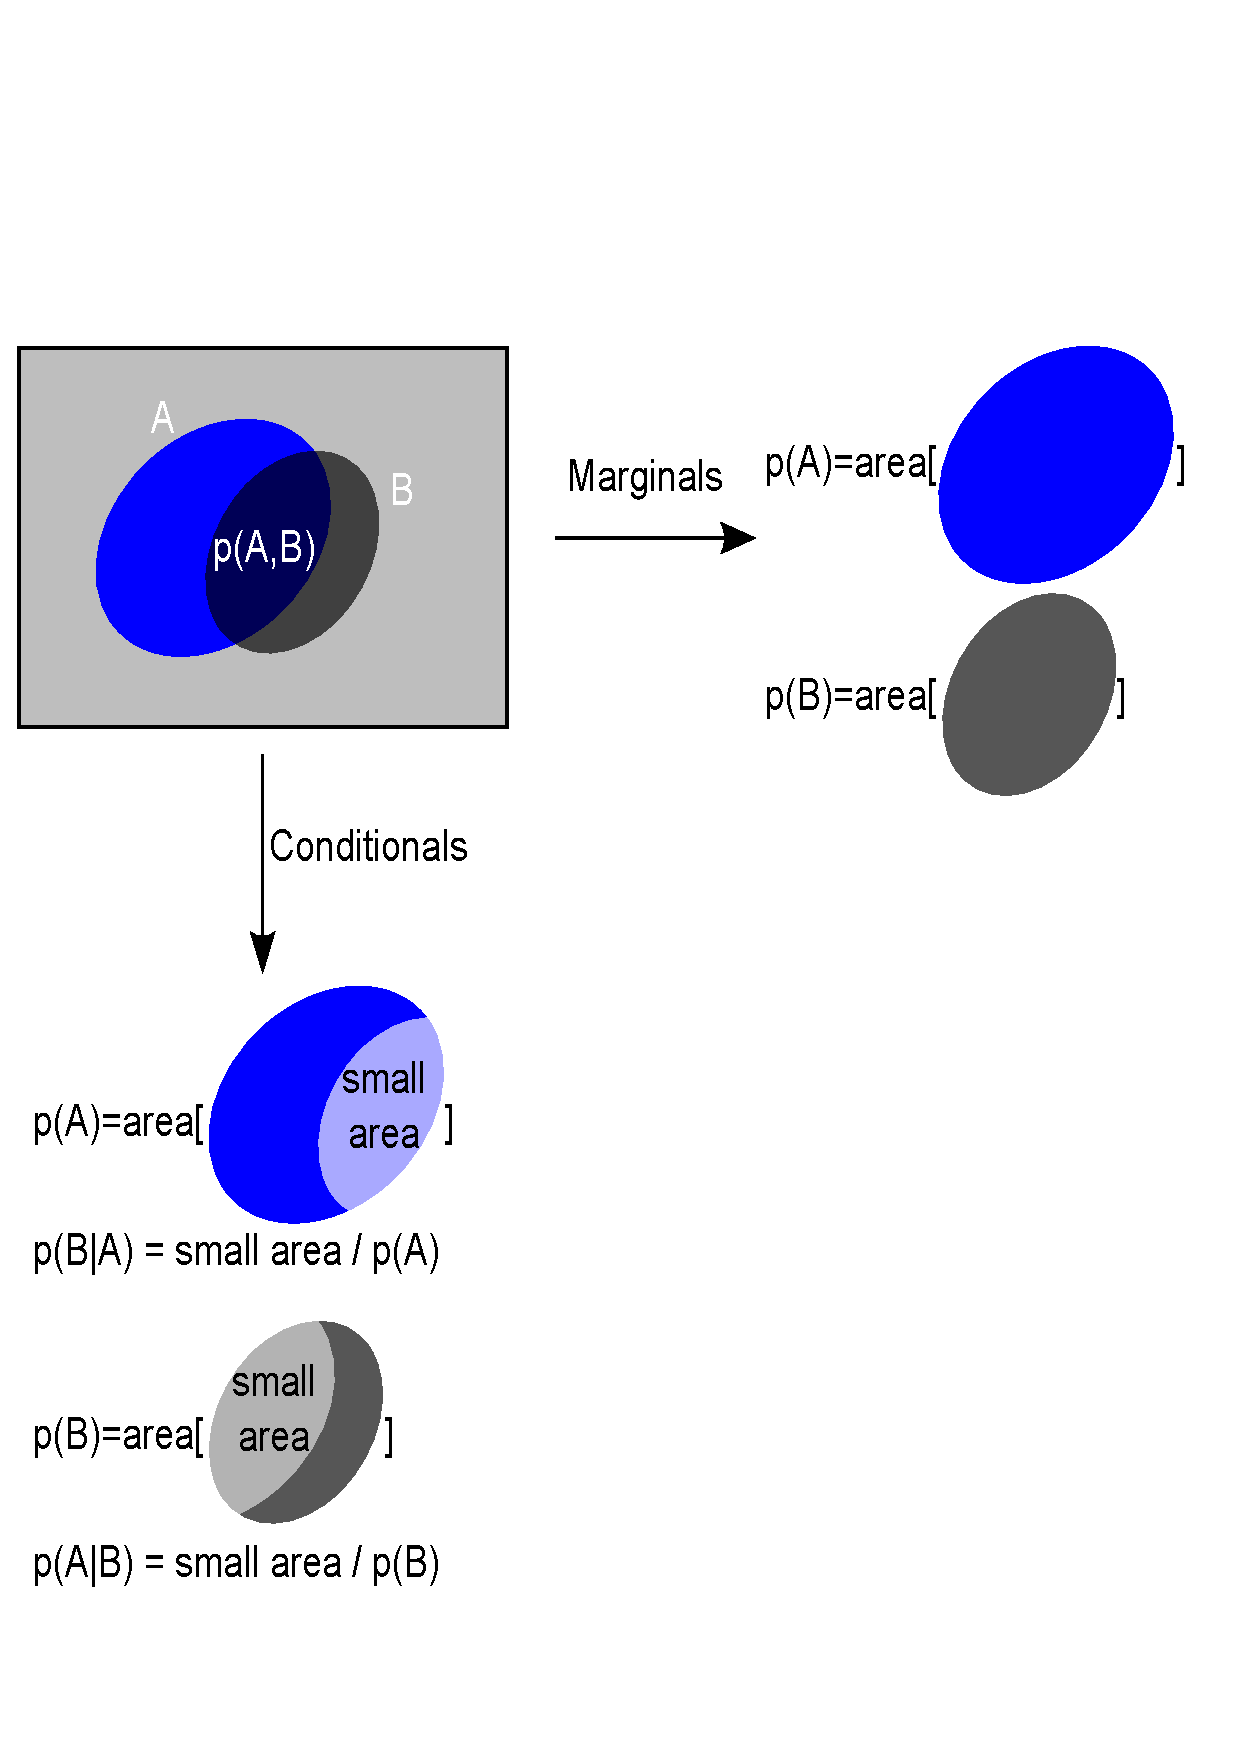
\includegraphics{Probability_Venn.pdf}}
\caption{A Venn diagram showing one way of interpreting marginal and conditional distributions for the horse racing example.}\label{fig:Probability_Venn}
\end{figure}

\subsection{Conditional distributions}\label{sec:Probability_conditionalDistributionIntro}
We sometimes only receive partial information by observing part of the system in which we are interested. In horses example, we might only see the result of one horse race, and on this basis update our probabilities of the other horse winning. Alternatively, in the foot size - literacy example described before, we might measure an individual's shoe size, and then want to obtain the updated probability distribution for literacy scores.

In probability, when we observe one variable, and reformulate the probability distribution for the other variable, we say that we are deriving the \textit{conditional} distribution of the latter. \textit{Conditional} refers to the fact that we are deriving the probability distribution of one variable, \textit{conditional} on the value of the other(s).

In each case, we have reduced some of the uncertainty in the system, by observing one of its characteristics. Hence in the two-dimensional examples described above the conditional distribution is only one-dimensional, because we are only now uncertain about one variable. 

Luckily, there is a simple rule that we can use to obtain the probability of one variable, conditional on the value of the other:

\begin{equation}\label{eq:Probability_conditionalProbability}
p(A|B) = \frac{p(A,B)}{p(B)}
\end{equation}

In (\ref{eq:Probability_conditionalProbability}), $p(A|B)$ refers to the probability of $A$ occurring, given that $B$ has occurred. In the right hand side of (\ref{eq:Probability_conditionalProbability}), $p(B)$ is the \textit{marginal} distribution of B occurring, and $p(A,B)$ is the joint probability of $A$ and $B$ occurring.

We can use (\ref{eq:Probability_conditionalProbability}) for the horses example to calculate the probability that \textit{given} that horse A wins, what is the probability of horse B also winning?

\begin{align}\label{eq:Probability_conditionalDiscreteCoins}
Pr(X_B=1|X_A=1) &= \frac{Pr(X_A=1,X_B=1)}{Pr(X_A=1)}\\
&= \frac{Pr(X_A=1,X_B=1)}{Pr(X_A=1,X_B=0)+Pr(X_A=1,X_B=1)}\\
&= \frac{\frac{50}{100}}{\frac{10}{100} + \frac{50}{100}}\\ 
&= \frac{5}{6}
\end{align}


In (\ref{eq:Probability_conditionalDiscreteCoins}), we have used the rule we discussed earlier for calculating marginal probabilities, shown in (\ref{eq:Probability_marginalDiscreteProbabilityTwoDimensions}), to calculate the denominator, $Pr(X_A=1)$ (allowing us to move from line 1 to 2).

Another way to see the workings of this calculation is shown in table \ref{tab:Probability_coinsConditionalDiscrete}. When we see that horse A wins, we essentially reduce our solution space to only the central column (highlighted in blue). Therefore we need to renormalise the solution space such that it has a probability of 1, by dividing each of its entries through by its original total of probabilities, 0.6; yielding the conditional probabilities shown in the right hand column of table \ref{tab:Probability_coinsConditionalDiscrete}.

\begin{table}[htbp]
  \centering
    \begin{tabular}{rrccr}
    \toprule
          &       & \multicolumn{2}{c}{\textbf{horse A}} &  \\
    \midrule
          &       & \textbf{0} & \textbf{1} & \multicolumn{1}{c}{\textbf{$Pr(X_B|X_A=1)$}} \\
    \multicolumn{1}{c}{\textbf{horse B}} & \multicolumn{1}{c}{\textbf{0}} & $\frac{30}{100}$   & {\color{blue}$\frac{10}{100}$ }   & \multicolumn{1}{c}{\textbf{=$\frac{10}{100}$ /$\frac{60}{100}$  = $\frac{1}{6}$ }} \\
    \multicolumn{1}{c}{} & \multicolumn{1}{c}{\textbf{1}} & $\frac{10}{100}$   & {\color{blue}$\frac{50}{100}$ }   & \multicolumn{1}{c}{\textbf{=$\frac{50}{100}$ /$\frac{60}{100}$  = $\frac{5}{6}$ }} \\
          & \multicolumn{1}{c}{\textbf{$Pr(X_A)$}} & \textbf{$\frac{40}{100}$ } & {\color{blue}\textbf{$\frac{60}{100}$ }} & \multicolumn{1}{c}{} \\
    \bottomrule
    \end{tabular}%
\caption{The highlighted region indicates the new solution space, since we know that horse A has won.}
\label{tab:Probability_coinsConditionalDiscrete}
\end{table}

The Venn diagram in figure \ref{fig:Probability_Venn} shows another way of interpreting conditional distributions. If we are told that horse B wins, then our event space collapses to only the area specified by B. The conditional probability, $p(X_A=1|X_B=1)$ is then simply given by the ratio of the area of overlap between A and B to the total area of B. This makes intuitive sense, since this is the only way that horse A can win, given that B has already won.

\begin{figure}
\centering
\scalebox{0.5} 
{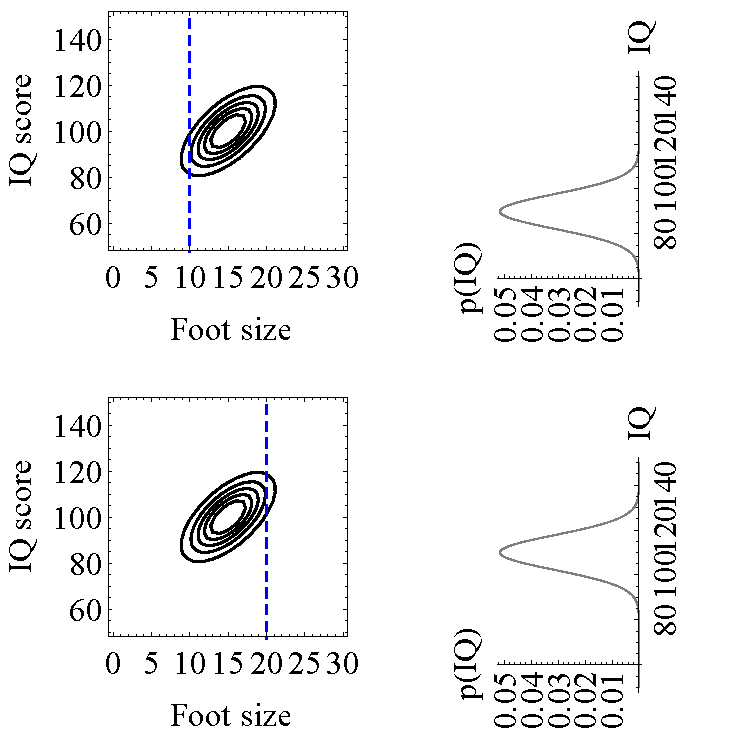
\includegraphics{Probability_footSizeIntelligenceConditional.pdf}}
\caption{The dashed blue lines indicate the new event space in each case. The height walked following these lines is related to the magnitude of the conditional distributions shown on the right.}\label{fig:Probability_footSizeIntelligenceConditional}
\end{figure}

We can also use (\ref{eq:Probability_conditionalProbability}) to allow us to calculate the conditional distribution of literacy scores for individuals after we have measured their shoe size. The only difference with the discrete example is that we now have to use an integral to work out the marginal probability for foot size; the denominator of (\ref{eq:Probability_conditionalProbability}). Figure \ref{fig:Probability_footSizeIntelligenceConditional} shows the conditional distributions traced out when we measure an individual's foot size to be 10cm and 20cm respectively. The blue dashed lines show the new event space, since we have lost our uncertainty over foot size in each of the cases. Therefore the heights traversed on the walk along these lines of constant foot size indicate the relative likelihood of different values of literacy scores. 

Add a stick man diagram.

\section{Higher dimensional probability densities: no harder than 2-D, just looks it!}
Now that we are equipped with the tools to calculate marginal and conditional distributions in two dimensions, we can use these to work with probability distributions that depend on any number of variables. Although formulae appear more complex, this is really just a result of having to keep track of each individual variable.

Imagine that we are told that there is another horse C, which comes from the same stable as horses A and B, which will compete in a third race, on the same day as the other two. This probability distribution could be represented by a 3-dimensional array, or alternatively as two separate tables of the same form as table \ref{tab:Probability_coinBiased}, one for each outcome for horse C's race. We could write this probability distribution as before, but with a third random variable $p(X_A,X_B,X_C)$. If we were only interested in the result of horses A and B, we can define a vector $\boldsymbol{Z}=(X_A,X_B)$, meaning that we could write our density as $p(\boldsymbol{Z},X_C)$. We can then just apply the same rule as before (in (\ref{eq:Probability_marginalDiscreteProbabilityTwoDimensions})) to get the marginal density, because our notation makes it look '2-dimensional':

\begin{align}\label{eq:Probability_3DDiscreteHorsesExample}
p(X_A,X_B) = p(\boldsymbol{Z}) &= \sum\limits_{X_C=0}^{1} p(\boldsymbol{Z},X_C)\\
&= p(\boldsymbol{Z},0) + (\boldsymbol{Z},1)
\end{align}

If we wanted to work out the new probabilities of the two horses winning \textit{conditional} on the fact that horse C has won, we can simply use our 'two-dimensional' notation, and equation (\ref{eq:Probability_conditionalProbability}):

\begin{align}
&p(X_A, X_B|X_C=1) = \frac{p(X_A,X_B,X_C=1)}{p(X_C=1)}\\
&= \frac{p(X_A,X_B,X_C=1)}{p(1,1,X_C=1) + p(1,0,X_C=1) + p(0,1,X_C=1) + p(0,0,X_C=1)}
\end{align}

Notice now however, that the denominator $p(X_C=1)$; representing the marginal probability of horse C winning is actually obtained by a sum over all the four possible ways this can occur: A and B winning, A winning and B not, B winning and A not, and finally both A and B losing\footnote{The notation is shortened to allow all the outcomes to be shown on a single line, so $p(X_A=1,X_B=1,X_C)=p(1,1,X_C)$, for example.}.

For another example, suppose that we have a continuous posterior density that is defined in terms of three person-specific variables, $p(IQ,FS,W)$; where $W$ represents the weight of an individual. If we wish to determine the posterior solely as a function of $IQ$ and $FS$, then we start by defining the parameter vector $\boldsymbol{\theta} = (IQ,FS)$, meaning we are left with $p(\boldsymbol{\theta},W)$. Note that all we have done is defined a new composite variable, $\boldsymbol{\theta}$. Now our density is of the '2-dimensional' form shown in (\ref{eq:Probability_marginalContinuousProbabilityTwoDimensions}), and we can apply this relation:\\

\begin{align}\label{eq:Probability_higherDimensionalMarginal}
p(IQ,FS) &= p(\boldsymbol{\theta})\\
&= \int\limits_{All\; W} p(\boldsymbol{\theta},W)\mathrm{d}W
\end{align}

If we wish to find the marginal distribution for $IQ$ \textit{only}, then all we do is integrate the resultant distribution in (\ref{eq:Probability_higherDimensionalMarginal}) with respect to $FS$.

We can use exactly the same trick to calculate the \textit{conditional} density of $IQ$ and $FS$, conditional on observing weight:

\begin{align}\label{eq:Probability_higherDimensionsConditional}
p(IQ,FS|W) &= p(\boldsymbol{\theta}|W)\\
&= \frac{p(\boldsymbol{\theta},W)}{p(W)}
\end{align}

In (\ref{eq:Probability_higherDimensionsConditional}), we have used (\ref{eq:Probability_conditionalProbability}) to arrive at the second line.

Finally, note that combining all parameters of interest into a single parameter vector $\boldsymbol{\theta}$ allows us to calculate \textit{marginal} and \textit{conditional} distributions for probability distributions that depend on an arbitrary number of parameters.

\section{Independence}\label{sec:Probability_independence}
If we think that there is a relationship between two random variables, then we say that they are \textit{dependent}. This does not necessarily mean \textit{causal} dependence, as it is sometimes supposed, in that the behaviour of variable $A$ affects the outcome of variable $B$. What it really means is that the value taken on by $A$ is informative for predicting $B$. 

An example of dependence might be the \textit{colour} and \textit{suit} of a playing card. If we are told that the colour of a playing card is $red$, this means that our other variable \textit{suit} is constrained to be either \textit{hearts} or \textit{diamonds}. In this case, knowing with certainty the value of the first variable, \textit{colour}, helps us to narrow down the list of outcomes of the second variable, \textit{suit} (see figure \ref{fig:Probability_IndependenceCards}).

\begin{figure}
\centering
\scalebox{0.3} 
{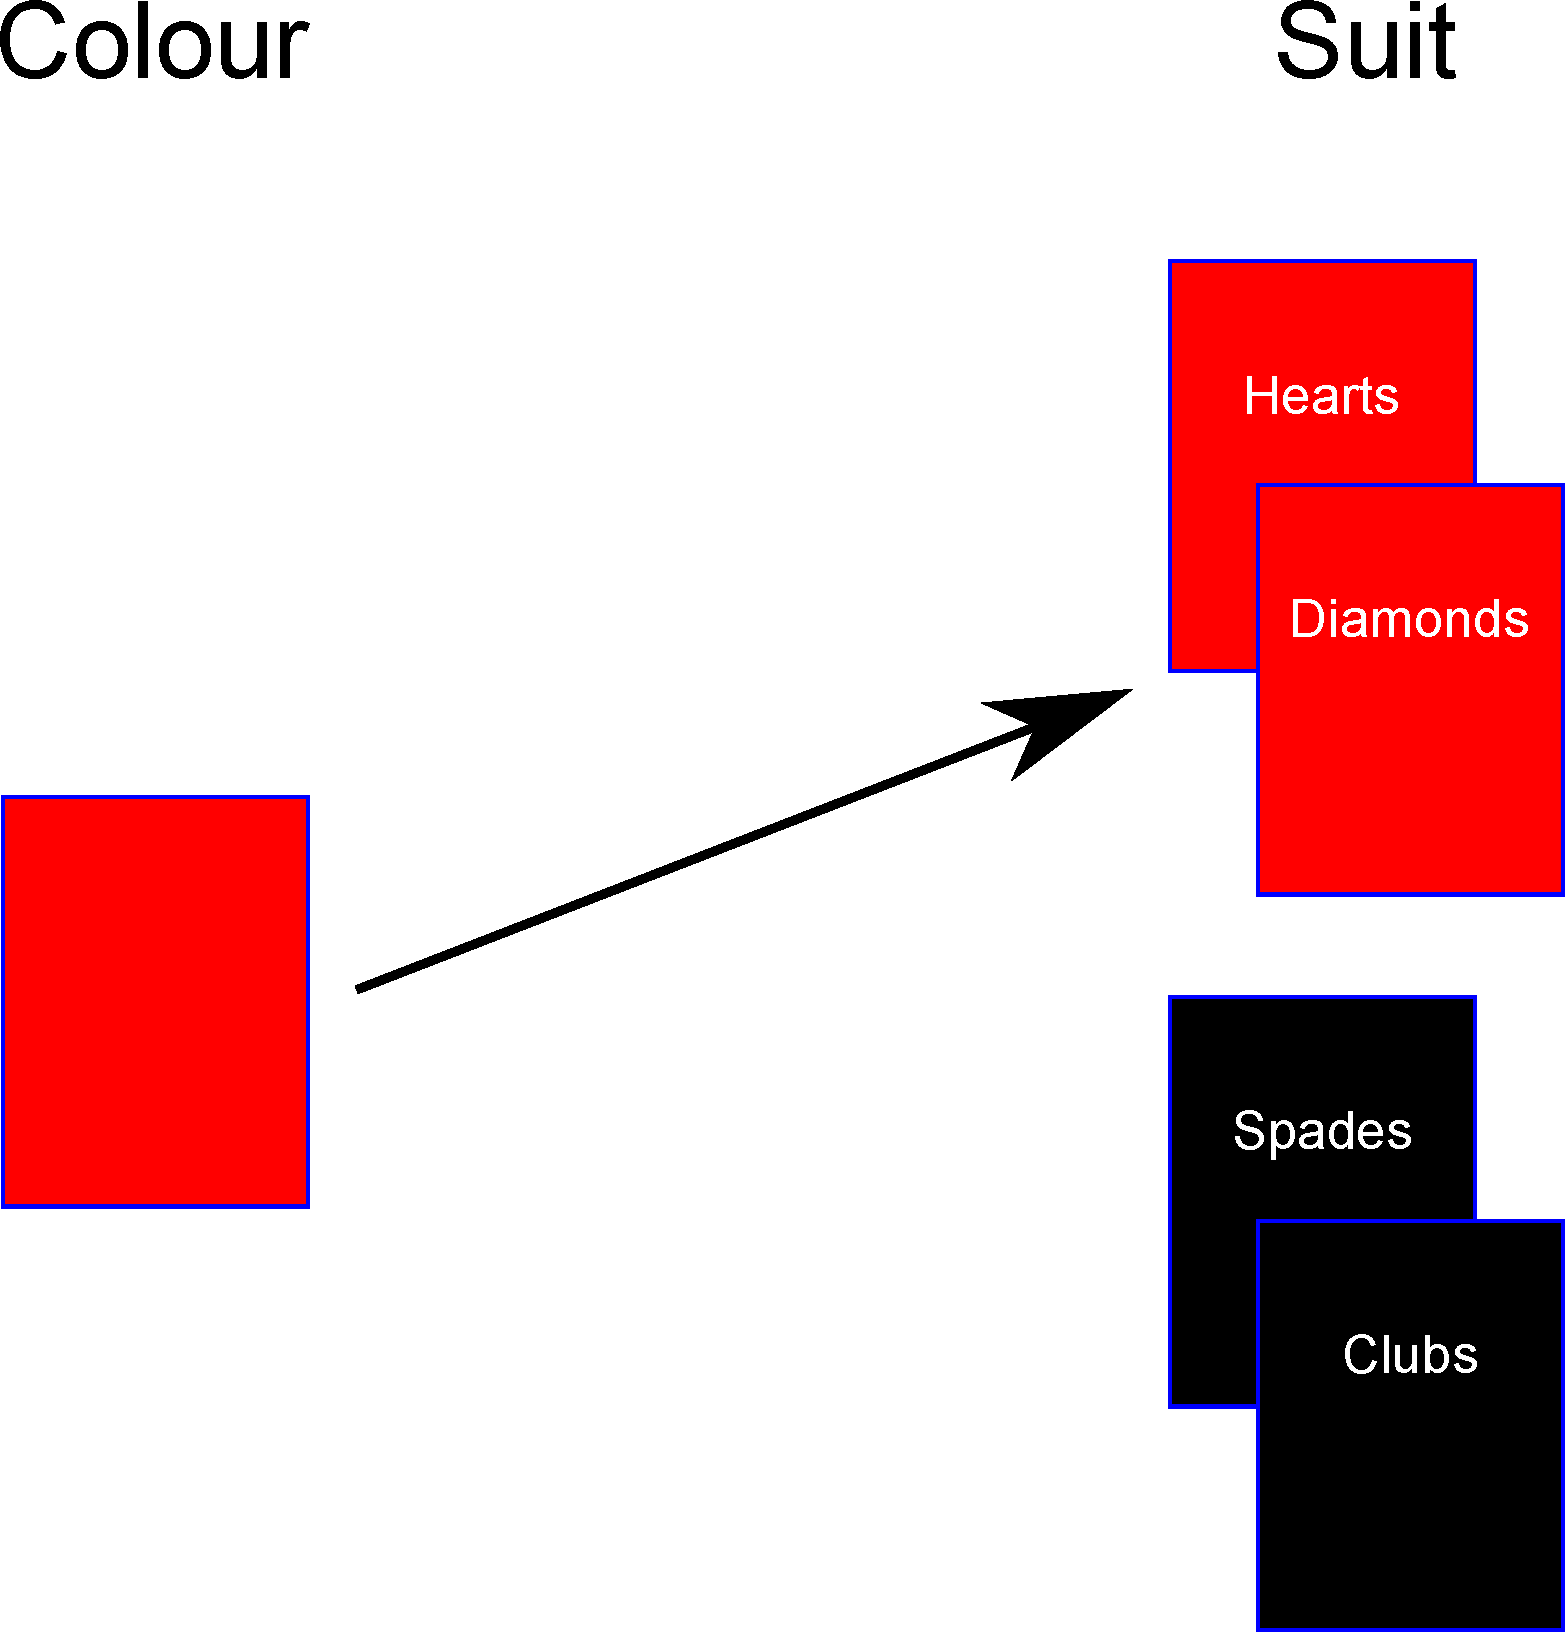
\includegraphics{Probability_IndependenceCards.pdf}}
\caption{Knowledge of the colour of a card provides information about the suit of the card. The colour and suit of a card are \textit{dependent}.}\label{fig:Probability_IndependenceCards}
\end{figure}

Another example of dependent variables, is the weather outside and the suntan of a particular, vein, individual\footnote{Discounting sunbeds.}. If it is sunny, then we assume it is more likely that an individual is tanned. Whereas, if the weather is cloudy, it is less so.

If two variables, $A$ and $B$ are \textit{disjoint}, then if one occurs, then the other cannot. In this case, it is often mistakenly believed that the variables are \textit{independent}, although this is very much not the case (see the left hand panel of figure \ref{fig:Probability_VennIndependence}). In this case, knowledge of variable $A$, provides significant information about variable $B$. If $A$ occurs, then we know for \textit{certain} that $B$ cannot!

\begin{figure}
\centering
\scalebox{0.4} 
{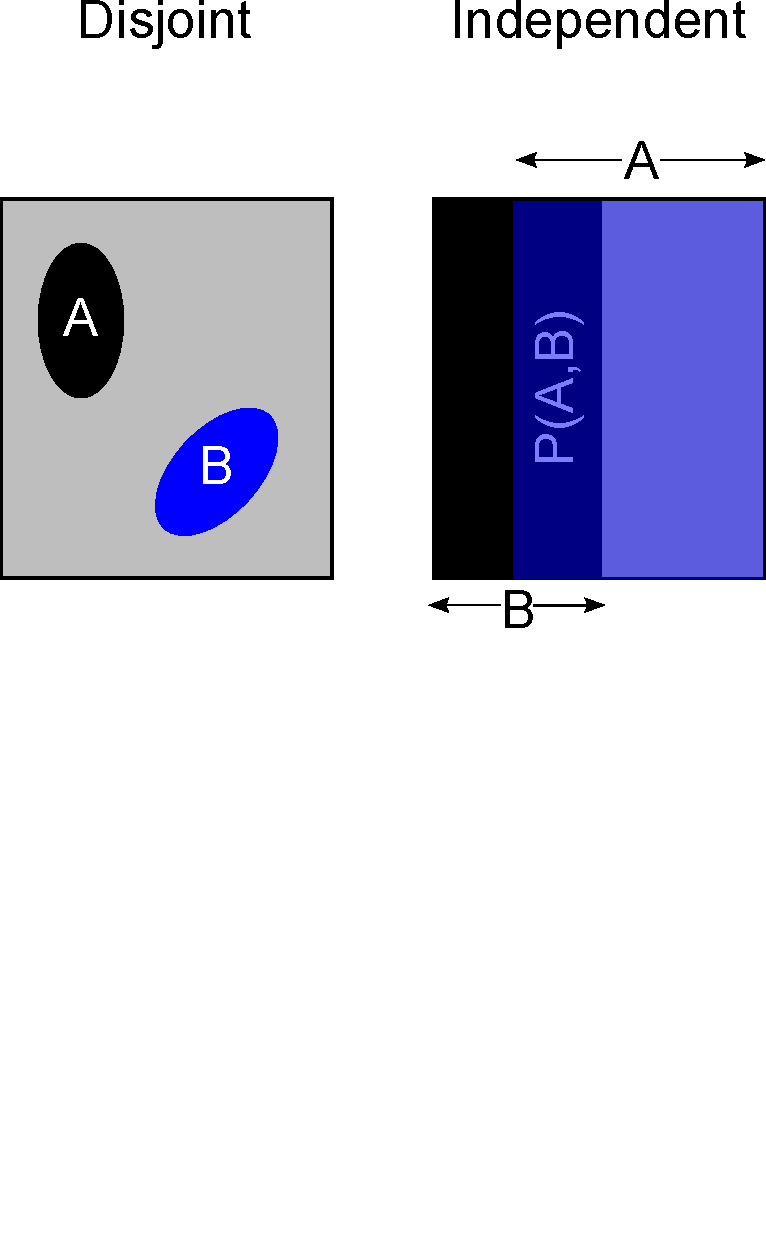
\includegraphics{Probability_VennIndependence.pdf}}
\caption{Venn diagram depictions of left: disjoint, and right: independent, events $A$ and $B$.}\label{fig:Probability_VennIndependence}
\end{figure}

By contrast, if two events are \textit{independent}, then knowledge of $B$ provides no additional information on $A$. Mathematically, this means that the conditional probability of $A$ is equal to the marginal:

\begin{equation}\label{eq:Probability_independentConditionalEqualMarginal}
p(A|B) = p(A)
\end{equation}

Using our conditional probability rule given in (\ref{eq:Probability_conditionalProbability}), we can then use this to rewrite the above as:

\begin{equation}\label{eq:Probability_independentConditionalEqualMarginal1}
\frac{p(A,B)}{p(B)} = p(A)
\end{equation}

In words, the ratio of the area of overlap between $A$ and $B$ to the area of $B$, is the same as the overall probability of $A$ (see the right hand panel of figure \ref{fig:Probability_VennIndependence}). This makes intuitive sense, since uncovering that $B$ has occurred (being in $B$) should result in no change to the probability of $A$ occurring (now $p(A|B)$).

Another way of stating independence that is commonly used, is obtained by multiplying (\ref{eq:Probability_independentConditionalEqualMarginal}) by its denominator:

\begin{equation}\label{eq:Probability_independentMultiplicationForm}
p(A,B) = p(A)\times p(B)
\end{equation}

To make this idea more concrete, we can think again of our horses example. Imagine that now are are considering two horses C and D, that come from separate stables, and race on different days. Using historical race results we have come up with the probability distribution shown in table \ref{tab:Probability_horsesIndependent}. 

We can use this table to test whether or not the results for the two horses are independent using (\ref{eq:Probability_independentMultiplicationForm}). We should be able to get the joint probabilities of both C and D winning from multiplying together the individual marginal densities:

\begin{align}
p(X_C=1,X_D=1) &= 0.3\\
&= p(X_C=1) \times p(X_D=1) 
&= 0.6 \times 0.5 = 0.3
\end{align}

which we see is true. We could similarly also validate this by checking the other three joint outcomes in the table, and find that this is the case.

\begin{table}[htbp]
  \centering
    \begin{tabular}{rrccr}
    \toprule
          &       & \multicolumn{2}{c}{\textbf{horse C}} &  \\
    \midrule
          &       & \textbf{0} & \textbf{1} & \multicolumn{1}{c}{\textbf{$Pr(X_D)$}} \\
    \multicolumn{1}{c}{\textbf{horse D}} & \multicolumn{1}{c}{\textbf{0}} & 0.2   & 0.3   & \multicolumn{1}{c}{\textbf{0.5}} \\
    \multicolumn{1}{c}{} & \multicolumn{1}{c}{\textbf{1}} & 0.2   & 0.3   & \multicolumn{1}{c}{\textbf{0.5}} \\
          & \multicolumn{1}{c}{\textbf{$Pr(X_C)$}} & \textbf{0.4} & \textbf{0.6} & \multicolumn{1}{c}{} \\
    \bottomrule
    \end{tabular}%
  \caption{The probability distribution for horses C and D. The marginal distribution of horses C and D are achieved by summing the values in each column or row respectively.}\label{tab:Probability_horsesIndependent}%
\end{table}%

\subsection{Conditional independence}\label{sec:Probability_conditionalIndependence}
In statistics we often come across situations where we suppose that observations are \textit{conditionally} independent. This is often swept under the carpet, and in discussion authors (falsely) state that the observations are \textit{independent}. Suppose that we work for the WHO, as an epidemiologist, and are interested in estimating the proportion of obese individuals within a distinct urban area. Within this area, we can suppose that there exists a true proportion of this condition, $\theta$. Suppose we select an individual uniformly at random from this population, and record their status, $X_1$, for this disorder. We then pick another individual, and record their status, calling it $X_2$. If we knew $\theta$, then we might suppose that the outcomes of these two picks are independent \textit{conditional} on this overall parameter. In other words, the outcome of the first sampling provides us \textit{no} further information on the disorder status of the second.

This conditional independence property is frequently represented in diagrammatic form of the type shown in figure \ref{fig:Probability_conditionalIndependence}. The arrows represent a dependency. When viewed in this light we see that it is incorrect to view the disease statuses of individuals 1 and 2 as \textit{fully} independent, since they are linked through a joint dependence on $\theta$. However, note that there is no direct arrow joining $X_1$ and $X_2$; this means that the random variables are \textit{conditionally} independent, when we allow for a joint dependence on $\theta$. 

\begin{figure}
\centering
\scalebox{0.4} 
{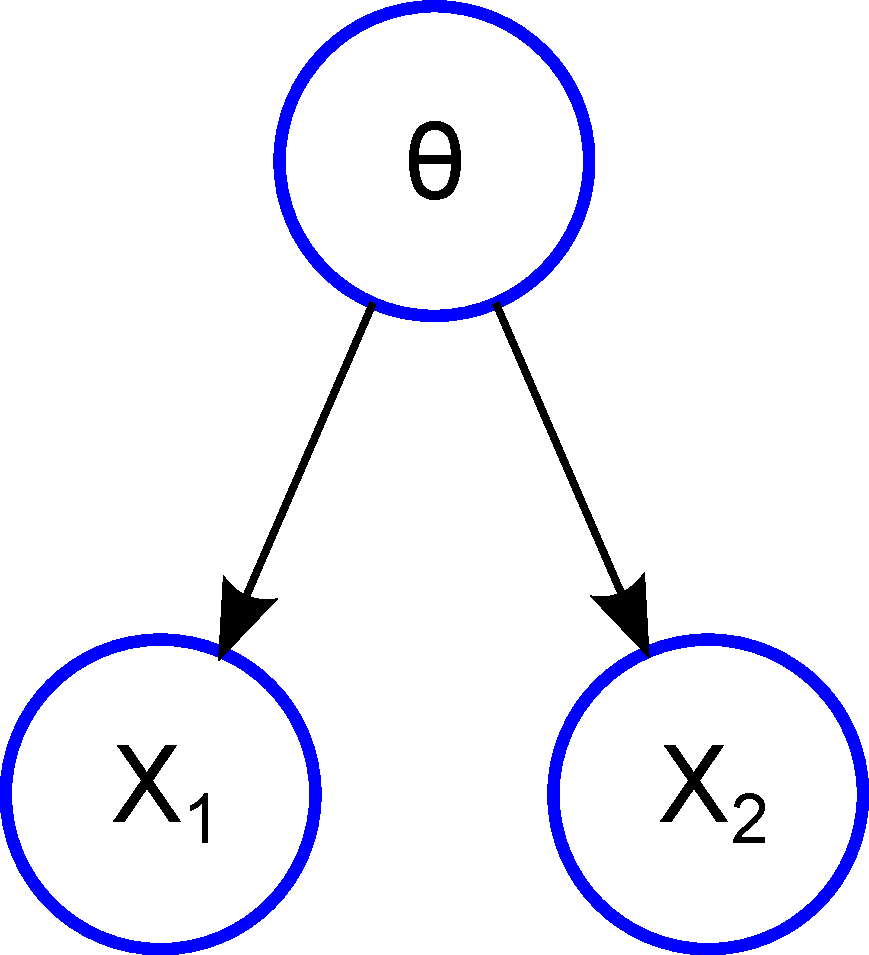
\includegraphics{Probability_conditionalIndependence.pdf}}
\caption{A diagrammatic depiction of conditional independence.}\label{fig:Probability_conditionalIndependence}
\end{figure}

\section{Central Limit Theorems}\label{sec:Probability_CLT}
Life is rarely simple, and in stating statistical models of phenomena we are attempting to at best, \textit{approximate} what is actually happening. In this environment, anything that brings a degree of certainty and coherence to our models is most welcome. 

Imagine that we are tasked with coming up with a model of probability for the \textit{mean} IQ test score in a particular school. Furthermore, as a simplification, we imagine that IQ is constrained to lie in the range $\left[0,300\right]$, and we believe that a reasonable probability distribution for an individual's test score is uniform on this range\footnote{Albeit this isn't a particularly good model, but suspend your disbelief for this thought experiment.} (see figure \ref{fig:Probability_CLTNormalSum}). We also suppose that individuals' scores are independent of one another.

Before we consider a sample size of $N$, we imagine that we only have a sample of two individuals, and we are asked to describe the distribution for the mean of their scores. If we use our assumption of uniformity, we might then ask, whether any mean scores are more likely than others, or are \textit{all} values equally likely, as per the individual case? We start by considering the extremes: there is only one way to achieve a mean test score of 300; both individuals would have to had scored 300. Similarly, to obtain a mean of 0, both individuals must score 0. However, consider obtaining a mean of 150. This could have been obtained with a number\footnote{Technically an infinity.} of combinations of scores, for example $\left(score_A,score_B\right)=$: $\left(150,150\right),\;\left(100,200\right),\;\left(125,175\right)$. Intuitively, there are many more ways of obtaining moderate values for the sample mean, that there are for the extremes. 

This tendency towards the centre increases the more values we sum over, since in order to get extreme values we would require \textit{more} individual scores to be simultaneously extreme; which is less likely. We can see this increasing central-tendency in figure \ref{fig:Probability_CLTNormalSum}, as the number of points being summed over increases.

However, we also see another tendency of the probability densities: \textit{an increasingly good fit of the normal distribution to these sample averages.} This approximation, it turns out, becomes \textit{exact} in the limit that we have an infinite sample, and is known as the \textit{Central Limit Theorem}. Although for our purposes, it will often be practically-exact if the sample size is sufficiently large. 

There are in fact a number of central limit theorems, of which we have only exposed you to the one for the average of independent, identically-distributed random variables\footnote{Known as the Lindeberg-Levy CLT. \textbf{Note: need an accent on the e.}}. However, what is important for you to note is that, whenever we have a number of factors, which additively result in an outcome, then an assumption of normality may be reasonable.

For example, there is an argument which would suggest that an individual's intelligence is the result of a number of factors including: un-bringing, genetics, life-experience, and health amongst others. Hence, we might tentatively propose that an individual's test score picked at random from the population would actually be normally-distributed! This is why we earlier mentioned that the assumption that individuals' test scores were uniform might not be reasonable.

\begin{figure}
\centering
\scalebox{0.4} 
{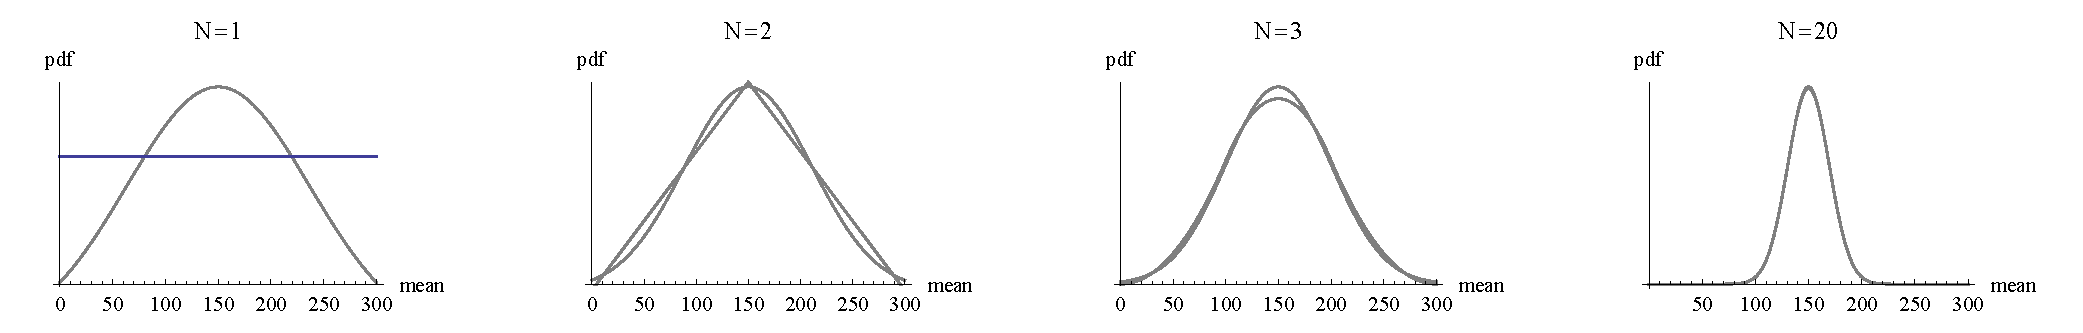
\includegraphics{Probability_CLTNormalSum.pdf}}
\caption{The convergence to a normal distribution for the mean of a sum of uniform distributions for IQ. The pdf for the average is shown in blue, with a normal distribution of the same mean and variance indicated in grey.}\label{fig:Probability_CLTNormalSum}
\end{figure}

\section{The Bayesian formula}\label{sec:Probability_BayesianFormula}
We first of all rewrite the conditional probability formula (\ref{eq:Probability_conditionalProbability}), regarding the probability of event A occurring, \textit{given} that event B has occurred:

\begin{equation}\label{eq:Probability_conditionalProbabilityAB}
p(A|B) = \frac{p(A,B)}{p(B)}
\end{equation}

However, we could also swap A and B around leading to the following for the probability of B \textit{given} that A has already occurred:

\begin{equation}\label{eq:Probability_conditionalProbabilityBA}
p(B|A) = \frac{p(B,A)}{p(A)}
\end{equation}

We however reason from the Venn diagram in figure \ref{fig:Probability_Venn}, that the overlap region of $p(A,B)$ really translated means, the probability of A \textit{and} B occurring. This means that this is exactly the same as the reverse; the probability of B \textit{and} A coinciding, $p(B,A)$. We can therefore rearrange (\ref{eq:Probability_conditionalProbabilityBA}) for this joint probability:

\begin{equation}\label{eq:Probability_jointConditionalProbability}
p(A,B) = p(B|A)\times p(A)
\end{equation}

We can use (\ref{eq:Probability_jointConditionalProbability}) to break down the probability of both A and B occurring into two steps. Firstly, for this to happen we require that A \textit{must} happen, with its corresponding probability $p(A)$. Then for both to occur, we straightforwardly require the probability of B occurring, \textit{given} that A has already occurred, which is given by $p(B|A)$. This reasoning provides a little intuition as to the workings of the conditional probability law that we wrote down in (\ref{eq:Probability_conditionalProbability}).

We can finally substitute (\ref{eq:Probability_jointConditionalProbability}) into the numerator of the fraction in (\ref{eq:Probability_conditionalProbabilityAB}), to yield the famous Bayesian formula!

\begin{equation}\label{eq:Probability_BayesianFormula}
p(A|B) = \frac{p(B|A)\times p(A)}{p(B)}
\end{equation}

The Bayesian formula importantly tells us how to correctly convert from $p(B|A)$ to its inverse $p(A|B)$, which is central to Bayesian statistics.

\subsection{The intuition behind the formula}
If we multiply both sides of (\ref{eq:Probability_BayesianFormula}) by $p(B)$, we arrive at the following alternative statement of Bayes' rule:

\begin{equation}\label{eq:Probability_BayesianIntuition}
p(A|B)\times p(B) = p(B|A)\times p(A) \;\;\;[= p(A,B)]
\end{equation}

In (\ref{eq:Probability_BayesianIntuition}), we have added the final part in square parentheses due to the reasoning of section \ref{sec:Probability_BayesianFormula}, that both sides are equivalent to the joint probability of A and B.

What the relation (\ref{eq:Probability_BayesianIntuition}) tells us however, is that there are two ways of arriving at this joint probability (see figure \ref{fig:Probability_BayesianIntuition}). The first way is given by the left hand side, and is due to B occurring, with probability $p(B)$, followed by A \textit{given} that B has occurred, with probability $p(A|B)$. An exactly equivalent way for both A and B to occur is given by the right hand side of the leftmost equals sign. Here we require that A occurs first, with probability $p(A)$, followed by B \textit{given} that A has occurred, with probability $p(B|A)$.

\begin{figure}
\centering
\scalebox{0.4} 
{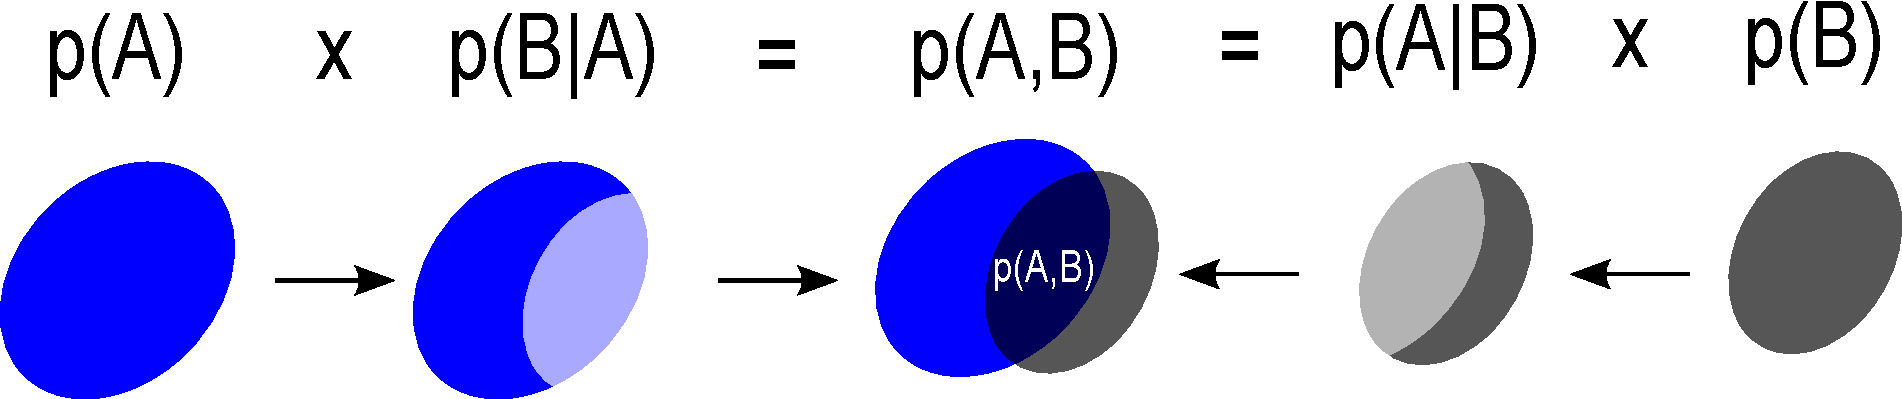
\includegraphics{Probability_BayesianIntuition.pdf}}
\caption{The two ways of arriving at the joint probability $p(A,B)$; providing some intuition behind Bayes' rule.}\label{fig:Probability_BayesianIntuition}
\end{figure}

\subsection{Breast cancer screeing}
Let's now make this discussion more concrete by means of an example. Let's imagine that we are an oncology doctor, working in breast cancer diagnosis. We suppose that out of all women aged forty who participate in screenings, about 1\% of them will have breast cancer at the time of testing. We suppose that the screening process is relatively robust, and it is known that for women who have breast cancer, the tests will indicate a positive result 80\% of the time. However, there is also the risk of false-positives, with 10\% of women without breast cancer also testing positive\footnote{We are not necessarily indicating clinically-up-to-date values, more we are using these example values to indicate the importance of reducing false-positives of any medical-test.}.

We now suppose that we are in the position where a woman has tested positive. What we would like to do, is work out the probability that she has breast cancer.

In the language of probability we would like to work out the conditional probability: $p(cancer|+ve)$. In words, the probability that she has breast cancer, \textit{given} that she has tested positive. However, summarising the information we currently have in probability language: $p(cancer)=0.01$, $p(+ve|cancer)=0.8$, and finally $p(+ve|no\; cancer) = 0.1$. How can we proceed? Bayes' formula to the rescue:

\begin{align}\label{eq:Probability_bayesBreastCancer}
p(cancer|+ve) &= \frac{p(+ve|cancer)\times p(cancer)}{p(+ve)}\\
&= \frac{p(+ve|cancer)\times p(cancer)}{p(+ve,cancer)+p(+ve,no\;cancer)}\\
&= \frac{0.8\times 0.01}{0.8\times 0.01 + 0.1\times 0.99} \approx 0.08
\end{align}

In (\ref{eq:Probability_bayesBreastCancer}), we got from the first line to the second by using (\ref{eq:Probability_marginalDiscreteProbabilityTwoDimensions}) to work out the marginal probability of an individual testing positive. The fact that the probability is so small is due to the risk of false positives (see video XXX for a fully-intuitive explanation of this), which produce many more positive diagnoses than the real-positives (because the risk of cancer is much lower than the probability of not having cancer).

\boxed{Video:} Make a video introducing Bayes' rule with Blair's decision to go to Iraq about WMDs. To coincide with the Chilcott enquiry (see Dad's email).

\section{The Bayesian inference process from the Bayesian formula}
In Bayesian statistics we aim to use probability distributions to describe all components of our system. Our starting point is Bayes' rule:

\begin{equation}\label{eq:Probability_BayesianFormula1}
p(A|B) = \frac{p(B|A)\times p(A)}{p(B)}
\end{equation}

In statistics we are typically looking to estimate a number of parameters, which we will from now on call $\theta$, which represent a component of a statistical model which we build to represent a particular phenomenon. These parameters can be real (such as the proportion of individuals within a given population that have a disease), or mere abstractions (for example the scale parameter of a hyper-distribution).

In Bayesian statistics, we want to update our beliefs about values of a parameter \textit{given} that we have obtained a particular sample of data. Being Bayesians, we would like to represent these beliefs via a probability distribution, which we write as $p(\theta|data)$. However, we can use (\ref{eq:Probability_BayesianFormula1}), (if we associate $A$ with $\theta$, and $B$ with the \textit{data}) to write:

\begin{equation}\label{eq:Probability_BayesianInferenceFormula}
p(\theta|data) = \frac{p(data|\theta)\times p(\theta)}{p(data)}
\end{equation}

Although we have straightforwardly made two substitutions to arrive at (\ref{eq:Probability_BayesianInferenceFormula}) from (\ref{eq:Probability_BayesianFormula1}), what have we gained by doing so? Also, what exactly do the terms on the right hand side actually mean? Although we introduced these in chapter \ref{chap:subjectiveFrequentistBayes}, we will spend the next part of this book examining each of these components in detail.

\section{Chapter summary}
The reader should now have developed a working understanding of probability distributions. Of particular importance in Bayesian statistics are the concepts of marginal and conditional distributions introduced in sections \ref{sec:Probability_marginal} and \ref{sec:Probability_conditionalDistributionIntro} respectively. If you do not feel fully confident with probability distributions, do not fret, since we will have ample opportunity to work with these mathematical objects in the next part of the book, where we provide an in-depth discussion of the various elements of the central formula of Bayesian inference: Bayes' rule.

\section{Chapter outcomes}
The reader should now be familiar with the following concepts:
\begin{enumerate}
\item The conditions under which a probability distribution is valid.
\item The difference between probability and probability density.
\item Summary distribution measures, and how to calculate them.
\item Two-or-more dimensional probability distributions.
\item Marginal distributions and how to calculate them.
\item Conditional distributions and how to calculate them.
\item Independence,
\item Central Limit Theorems.
\item The Bayesian formula.
\end{enumerate}

\section{Problem set}
\subsection{The expected returns of a derivative}
The returns of a particular stock are thought to be well described by a log-normal distribution:

\begin{equation}
log(S_t) \sim N(\mu,\sigma^2)
\end{equation}

\subsubsection{What are the expected returns of the stock?}
\subsubsection{What are the variance in returns?}

The performance of a particular type of derivative is given by the following formula:
\begin{equation}
D_t = S_t^2
\end{equation}

\subsubsection{Would you expect the return to be equal to the mean of the original stock squared? If not, why not?}
Note to myself: the convexity of the squared function means that it is greater.
\subsubsection{What would be a fair price to pay for this derivative?}

An alternative stock is probabilistically related to the performance of $S_t$:

\begin{equation}
R_t \sim N(S^2,1)
\end{equation}

\subsubsection{What is a fair price to pay for this stock?}
\subsubsection{Which asset is more risky, $D_t$ or $R_t$?}

The data file XXX contains Stock return data for the stock $S_t$. A way to estimate the parameter is via a method known as \textit{method of moments}. Here, we might estimate the parameters $\mu$ and $\sigma$ by equating the sample mean and variance, to the \textit{population} quantities we believe our process abides by.

\subsubsection{Use \textit{method of moments} to estimate $\mu$ and $\sigma$. Note: this requires use of a computer with mathematical software, as analytic solutions aren't possible.}

\subsubsection{Compare the estimated model with the data.}
\subsubsection{Is the model a reasonable approximation to the data generating process?}
\subsubsection{If not, suggest a better alternative.}

\subsection{The boy or girl paradox}
Suppose we are told the following information\footnote{First introduced by Martin Gardner in 1959.}:

Mr Bayes has two children. The older child is a girl. What is the probability that both children are girls?
Mr Laplace has two children. At least one of the children is a girl. What is the probability that both children are girls?

\subsection{The Bayesian game show}
A game show presents contestants with four doors: behind one of the doors is a car worth \$1000; behind another is a forfeit whereby the contestant must pay \$500 out of their winnings thus far on the show. Behind the other two doors there is nothing.

The order of the game is thus:
\begin{enumerate}
\item The contestant chooses one of four doors.
\item The game show host opens one of the empty doors.
\item The contestant is given the option of changing their choice to one of the two remaining doors.
\item The contestant's final choice door is opened, either to their delight (a car!), dismay (a penalty), or indifference (nothing).
\end{enumerate}

Assuming that:

\begin{enumerate}
\item The contestant wants to maximise the probability that they win the car.
\item The contestant is risk averse.
\end{enumerate}

Find the optimal strategy for the contestant.

If you are unsure as to how to proceed, why not simulate the game using a computer. The program should only be a few lines, and might provide you with some intuition as to what is happening.

\subsection{Blood doping}
Suppose as a benign omniscient observer, we tally up the historical cases where professional cyclists used/didn't-use blood doping, and either won or lost a particular race. This results in the probability distribution shown in table \ref{tab:Probability_PS_bloodDoping}.

\subsubsection{What is the probability that a professional cyclist wins a race?}
\subsubsection{What is the probability that a cyclist wins a race given that they have cheated?}
\subsubsection{What is the probability that a cyclist is cheating given that he wins?}

\begin{table}[htbp]
  \centering
    \begin{tabular}{ccc}
    \toprule
          & \textbf{Lost} & \textbf{Won} \\
    \midrule
    \textbf{Clean} & 0.7   & 0.05 \\
    \textbf{Doping} & 0.15  & 0.15 \\
    \bottomrule
    \end{tabular}%
    \caption{The historical probabilities of behaviour and outcome for professional cyclists.}
  \label{tab:Probability_PS_bloodDoping}%
\end{table}%

Now suppose that drug testing officials have a test which is relatively accurate in finding cheats. It accurately indicates a blood-doper 90\% of the time. However, it incorrectly indicates a positive for clean athletes 5\% of the time. 

Should the officials test all the athletes or only the winners, for the cases when:

\begin{enumerate}
\item They care only about the proportion of people correctly identified as dopers.
\item They want only to minimise the proportion of falsely accused athletes.
\item They care only about the \textit{number} of people correctly identified as dopers.
\item They care five times about the \textit{number} of people who are falsely identified as they do about the \textit{number} of people who are correctly identified as dopers.
\item What factor would make the officials choose the other group? (By factor, we mean the number 5 in the previous question.)
\end{enumerate}


\part{Understanding the Bayesian formula}\label{part:bayesianFormula}
\section{Part mission statement}
This part introduces the reader to the various elements of the Bayesian inference formula: the posterior, the likelihood, the prior and the denominator.

\section{Part goals}
The goal of Bayesian inference is to calculate the posterior distribution for parameters of interest. This distribution is the starting point for making decisions, and drawing conclusions about situations under examination. It is thus important to understand why this part of Bayes' formula is so useful, and hence we devote chapter \ref{chap:posterior} to this purpose. The first term on the right-hand-side of Bayes' formula that we encounter is the likelihood function, introduced in chapter \ref{chap:Likelihoods}. These functions/distributions allow for variance in the data, even if the parameters are fixed. This variance is what classical statisticians call sampling variation. Importantly, likelihood functions are not valid probability distributions, and are actually the inverse of what we desire. Bayes' rule essentially tells us how to invert these distributions in order to get our desired distributions - the posterior. However, in order to invert the likelihood, we need to specify the final piece of the puzzle - the prior distribution. This is a measure of our pre-data confidence across all the possible values of the parameter. We are required to specify this term, since Bayes' rule only tells us how to \textit{update} our beliefs, not how to specify them in the first place. Priors are without doubt the most controversial part of Bayesian inference, although as we have seen in chapter \ref{chap:subjectiveFrequentistBayes}, and we advocate in chapter \ref{chap:Prior}, this criticism is unwarranted. The final part of the formula - the denominator - is determined fully by our choice of likelihood and prior. However, this predetermination does not make out lives simple, and we shall see that the difficulty in evaluating this term, along with similar expressions, motivates the computational methods introduced in part \ref{part:computationalBayes}.

\chapter{The posterior - the goal of Bayesian inference}\label{chap:posterior}
\section{Chapter Mission statement}
At the end of this chapter the reader will understand the central importance, and use of the posterior probability distribution in Bayesian statistics.

Insert a graphic with the likelihood part of Bayes' formula circled, as in the equation shown below for the part highlighted in blue.

\begin{equation}
{\color{blue}p(\theta|data)} = \frac{p(data|\theta)\times p(\theta)}{p(data)}
\end{equation}\label{eq:Posterior_BayesHighlighted}

\section{Chapter goals}
Calculating the posterior distribution for a model's parameters is the focus of Bayesian analysis. This \textit{probability distribution} which results from the application of Bayes' rule (see \ref{eq:Posterior_BayesHighlighted}) can be used to infer the effects of given variables, to forecast, compare different models of phenomena, as well as test its own foundations! In order to do justice to the multitude of uses of the posterior distribution, it is necessary that the reader is familiar with the basics of probability distributions explained in chapter \ref{chap:subjectiveFrequentistBayes}. 

\section{Expressing uncertainty through the posterior probability distribution}\label{sec:Posterior_parameterUncertainty}
Unlike looking out the window, getting exam results, or playing a hand at blackjack, we frequently in inference never learn the \textit{true}\footnote{Whether a true value for a parameter actually exists we leave until section \ref{sec:Posterior_parametersExist}.} state of nature. The uncertainty here is both in the future and \textit{present}; the latter meaning we are unable to perfectly measure the state of the world today, and hence cannot hope to perfectly know the former.

A way of representing our ignorance, or uncertainty in a parameter's value is through probability distributions. For example, suppose that we wanted to know the proportion of individuals that would vote for the democrats in an upcoming election. We might, on the basis of past exit poll surveys, calculate a posterior\footnote{Via Bayes' rule - don't worry if you don't know how to do this, that is the goal of this whole first part!} uncertainty which is represented by the probability distribution which is shown in figure \ref{fig:Posterior_electionProportion}. 

\begin{figure}
\centering
\scalebox{0.5} 
{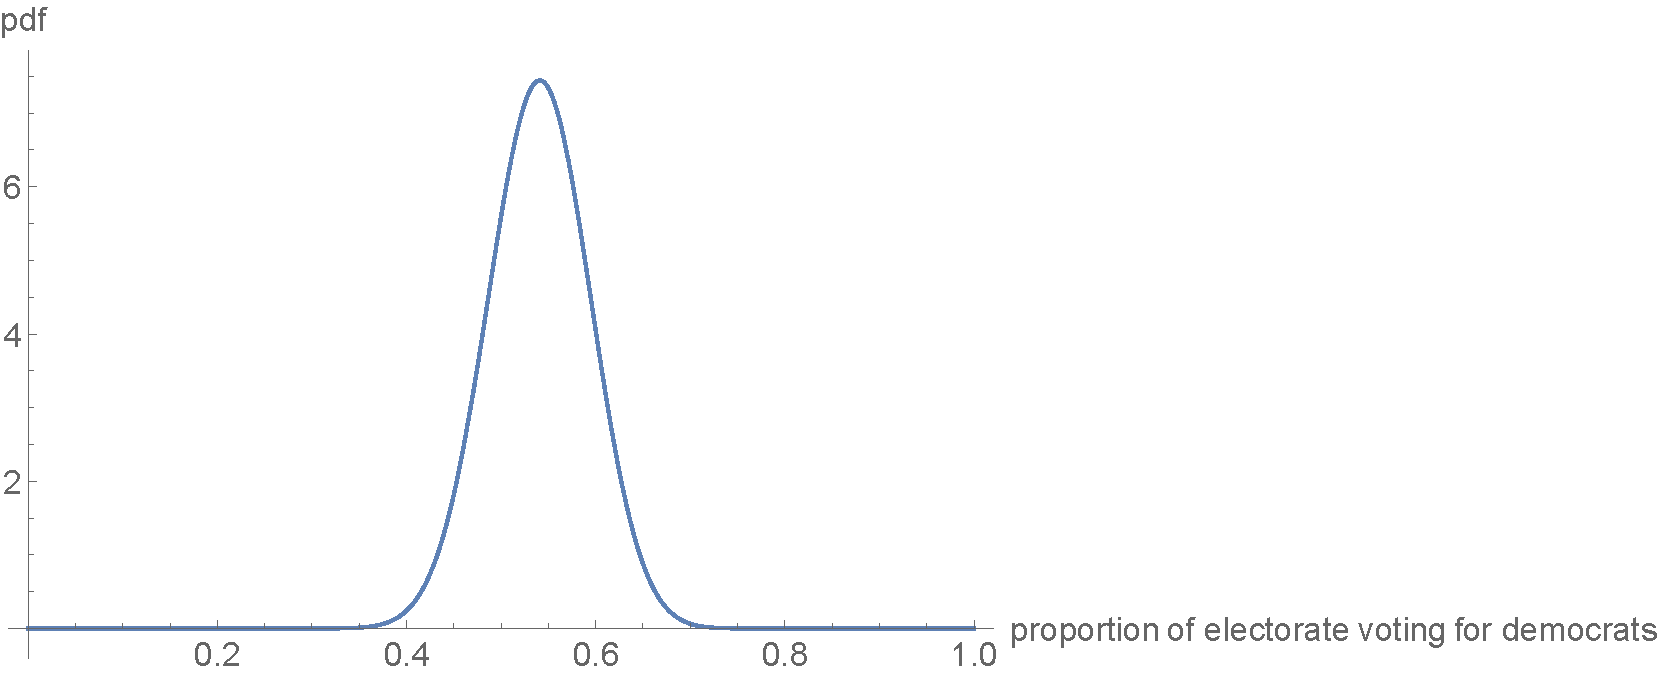
\includegraphics{Posterior_electionProportion.pdf}}
\caption{A probability distribution representing uncertainty over the proportion of the electorate that will vote for the Democrats in an upcoming election.}\label{fig:Posterior_electionProportion}
\end{figure}

How can we interpret the probability distribution shown in figure \ref{fig:Posterior_electionProportion}? And further, how can we use it to express our uncertainty to a non-mathematician? 

Often we describe a distribution by its summary characteristics. These are aspects of the distribution that we commonly want to know. For example, we normally want to know the \textit{mean} value of a parameter. This is a measure of central tendency of our estimates, that is essentially a weighted mean (where the weights are provided by the values of the probability density function). If we have the mathematical description of the distribution shown in figure \ref{fig:Posterior_electionProportion}, we can calculate this by simply finding its mean, by taking the expectation:

\begin{equation}
\mathbb{E}[\theta] = \int\limits_{0}^{1} p(\theta)\theta \mathrm{d}\theta = 54\%
\end{equation}

This provides a point estimate of the proportion of individuals - 54\% - that we expect to vote for the Democrats, which may be a useful piece of information to pass on to an interested party. 

A point estimate of the proportion of individuals that we expect to vote for the Democrats is not useful in itself, (and quite dangerous to pass on), without some measure of our inherent confidence/uncertainty in this particular value. One measure of uncertainty in a parameter's value is its variance:

\begin{equation}
var(\theta)=  \int\limits_{0}^{1} p(\theta)(\theta-\mathbb(E[\theta])^2 \mathrm{d}\theta
\end{equation}

In many cases, it is easier to understand the meaning of uncertainty if it is expressed in the same units as the mean, which we do by taking the square root of the variance, yielding 5.3\% for the case of figure \ref{fig:Posterior_electionProportion}. A larger variance indicates that we view a wider range of outcomes as being feasible. In this case, a wider variance would mean that we would be less surprised if the electorate voted in the Republican party. 

In sections \ref{sec:Posterior_HDI} and \ref{sec:Posterior_CPI} we will introduce other summary measures of distributions, that are also often presented in research articles, and books. However, the important thing to note is that all of these are derived from the posterior distribution for our parameters. 

Another example of the use of posteriors can be illustrated by a regression example. Suppose that we are investigating the effect of military participation on lifetime earnings\footnote{See Angrist's fantastic 1990 article for a detailed study of this effect for Vietnam war veterans \cite{angrist1990lifetime}.}. We suppose that the effect is, on average, negative due in part to the psychological stresses of warfare. We also suppose that the effect can be modelled as being linear, and hence our relationship of interest can be represented as:

\begin{equation}\label{eq:Posterior_militaryParticipation}
LI_i = \alpha + \beta MP_i + \epsilon_i
\end{equation}

where we expect that $\beta$ is negative. Here $\epsilon_i$ represents the myriad of other factors that are important for determination of an individual's income.

If we formulate a Bayesian model, with a given prior and likelihood, then we might end up with a posterior density for $\beta$, that is shown in figure \ref{fig:Posterior_regressionMilitaryParticipation}. We can use this density to help us to calculate the posterior probability that the given parameter is in fact non-negative, by finding the area under the curve corresponding to $\beta\geq 0$ (shown as the shaded region in figure \ref{fig:Posterior_regressionMilitaryParticipation}), which we find in this case to be approximately 25\%. This suggests that we are not all that confident in the fact that the parameter is negative (at 75\%), and cannot reasonably go along with our hypothesis.

\begin{figure}
\centering
\scalebox{0.5} 
{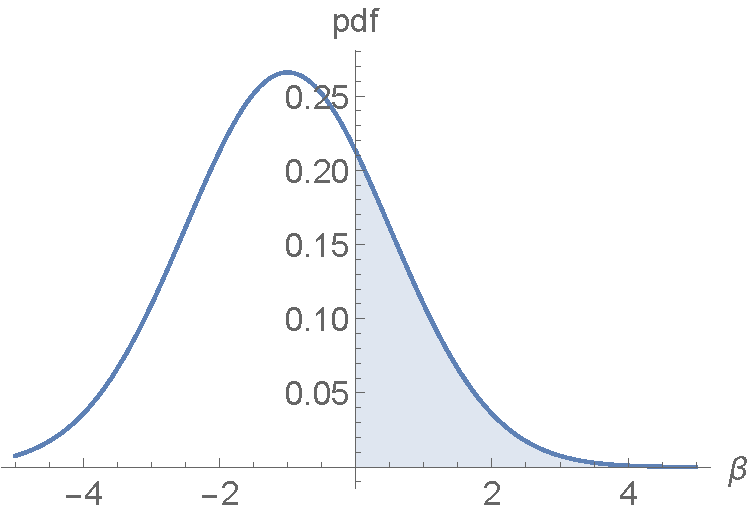
\includegraphics{Posterior_regressionMilitaryParticipation.pdf}}
\caption{An estimated posterior probability distribution for the parameter $\beta$ in (\ref{eq:Posterior_militaryParticipation}). The shaded region represents the posterior probability that the parameter is positive.}\label{fig:Posterior_regressionMilitaryParticipation}
\end{figure}

\subsection{Bayesian coastguard: introducing the prior and the posterior}
Imagine you are stationed in a radio control tower at the top of a steep cliff, in the midst of a stormy night. The tower received a distress call over radio from a ship - The Frequentasy - which has got engine trouble, somewhere out in the bay. It is your job to direct a search helicopter to rescue the poor sailors.

When you first receive the weak crackled radio signal, you are not made aware of their location. However, you know that the boat must be somewhere in the bay, less that 25km away from the tower, since this is the maximum possible range of the radio. Accordingly, you represent these views via the prior shown in the left hand panel of figure 1 (fairly flat prior in a circle from the tower, perhaps going down to zero gradually at 25km). The search area represented by this prior is currently far too wide for a rescue crew to reach the flagging ship in time!

In an attempt to improve the odds, you radio to the ship, and ask that they switch on their emergency transmitter. After radioing a number of times, you receive a weak signal, which you feed into the computer, resulting in a posterior probability density for the ship's location shown in the central panel of figure 1. (This panel shows a broadly peaked density along a line from the ship to the station, near a particular location 15km away).

The trouble is, the search area inferred from the aforementioned posterior is still wide. Luckily for the crew however, another nearby radio station has also picked up the signal, and they share this information with you. Finally, feeding this information into the computer, you obtain a final estimation of the ship's location, shown in the right hand panel of figure 1. 

Since there is only a small area of high density, you direct the rescue helicopter to search this area, and they find the captain and crew in time.

\begin{figure}
\centering
\scalebox{0.2} 
{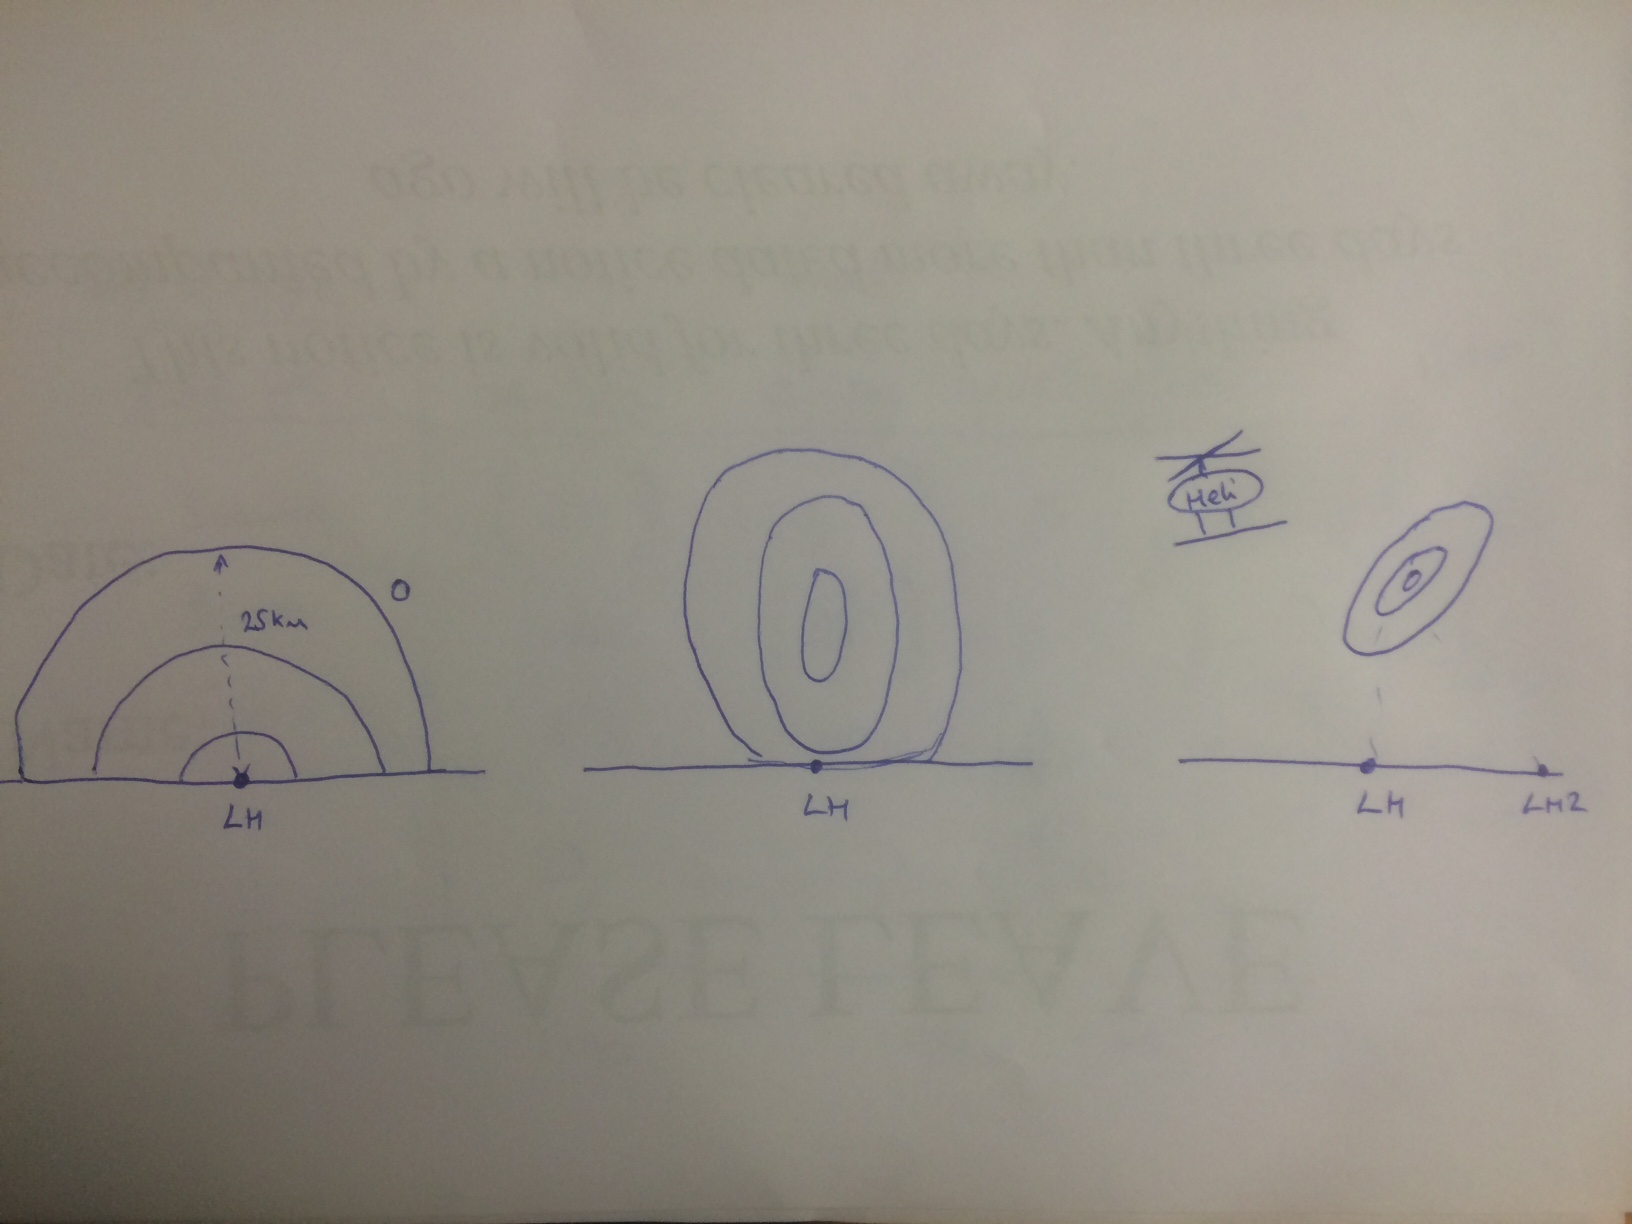
\includegraphics{Posterior_bayesianLighthouse.jpg}}
\caption{Three plots. Left hand plot is a contour plot of probability radiated symmetrically in a semi-circle away from the radio control tower, with the density declining to zero at 25km. The middle plot shows a contour plot of probability, with a higher density towards the centre of the diagram (here the densities are still relatively smooth, indicating high uncertainty). The final plot shows a definite peak in intensity around a particular point about 10km away from the coast, just right of centre. The different contours will be increasing shades of a particular colour.}\label{fig:Posterior_bayesianLighthouse}
\end{figure}

\subsection{Bayesian statistics: updating our pre-analysis uncertainty}
In Bayesian statistics the posterior distribution summarises the combination of our pre-study, and post-analysis knowledge about a given situation, and is used as the starting point for any further analysis or descriptions of our results. In order to calculate it, we need to choose a probability model, which in turn defines uncertain parameters, over which we place priors. The model also provides us with a \textit{likelihood} of the data we obtained. The priors and likelihoods are then combined in a certain way - using Bayes' rule - to yield the posterior distribution.

\begin{equation}
prior + data \rightarrow posterior
\end{equation}

In the Bayesian coastguard example, we started off with a fairly wide prior, since we were quite uncertain of the boat's location. We then fed the data from the ships' emergency transmitter, along with the prior, into the computer - which uses Bayes' rule - to provide an updated estimate of the ship's location. We actually went through this process twice, to emphasise the fact that Bayes' rule can be used iteratively to update knowledge about an uncertain situation.

Statistical inference is useful whenever there is uncertainty regarding a parameter of interest. Bayesians use the posterior distribution, and various summaries of it, in order to describe the degree of uncertainty regarding a parameter. Before we delve too deep though, it is useful to take a step back, and ask the somewhat philosophical question, 'Do parameters actually exist?' 

\subsection{Do parameters actually exist and have a point value?}\label{sec:Posterior_parametersExist}
For Bayesians, the parameters of the system are taken to vary, whereas the known part of the system - the data - is taken as given. Whereas Frequentist statisticians view the unseen part of the system - the parameters of the probability model - as being fixed, whereas the known parts of the system - the data - as varying. Whether you agree with one of these views more than the other mainly comes down to how you want to interpret the parameters of a given statistical model. 

The Bayesian perspective on parameters can be viewed as having a duality of meaning. Either we view the parameters as truly \textit{varying}, or we view our knowledge about the parameters as imperfect. The fact that we will get different estimates of parameters from different studies can be taken to reflect either of these two views. Either we view the parameters of interest as varying - taking on different values in each of the samples we pick (see the bottom panel of figure \ref{fig:Posterior_manyWorldsDoParametersExist}). Alternatively, we can view our uncertainty over a parameter's value as the reason we will estimate slightly different values in different samples. This uncertainty is thought of as decreasing as we collect more data (see the middle panel of figure \ref{fig:Posterior_manyWorldsDoParametersExist}). Bayesians are more at ease with using parameters as a means to an end - taking them not as real immutable constants, but as tools from which to make inferences about a given situation.

The Frequentist perspective is less flexible, and assumes that these parameters are constant; alternatively representing the average of a long run - typically infinite number - of identical experiments. There are occasions when we might think that this is a reasonable assumption. For example, if our parameter represented the proportion of the electorate that voted for the Democrat party in the last election, or the probability that an individual taken at random from the UK population will have dyslexia. In both these examples, it is reasonable to assume that there is a \textit{true}, or fixed \textit{population} value of the parameter of question. Whilst the Frequentist view might be in some ways reasonable here, the Bayesian view easily extends here to encompass these two situations by assuming that we are uncertain about the value of these fixed parameters before we measure them, and using a probability distribution to represent this lack of perfect knowledge. 

However, there are circumstances when the Frequentist view runs into trouble. When we are estimating parameters of an arbitrarily complicated distribution, we normally do not view them as actually existing. Unless you view the universe as being built from mathematical building blocks\footnote{See \cite{tegmark2014our} for an interesting argument for this hypothesis}, then it seems incorrect to assert that a given parameter has any deeper existence than that with which we endow it. The less restrictive Bayesian perspective here seems more reasonable.

The Frequentist view of parameters as a limiting value of an average across an infinity of identically repeated experiments (see the top panel of figure \ref{fig:Posterior_manyWorldsDoParametersExist}) also runs into difficulty when we think about one-off events, such as the 2016 US Presidential Election result. Any parameter we wish to estimate about such an event cannot easily be existentially justified on these grounds, since elections cannot be rerun.


\begin{figure}
\centering
\scalebox{0.2} 
{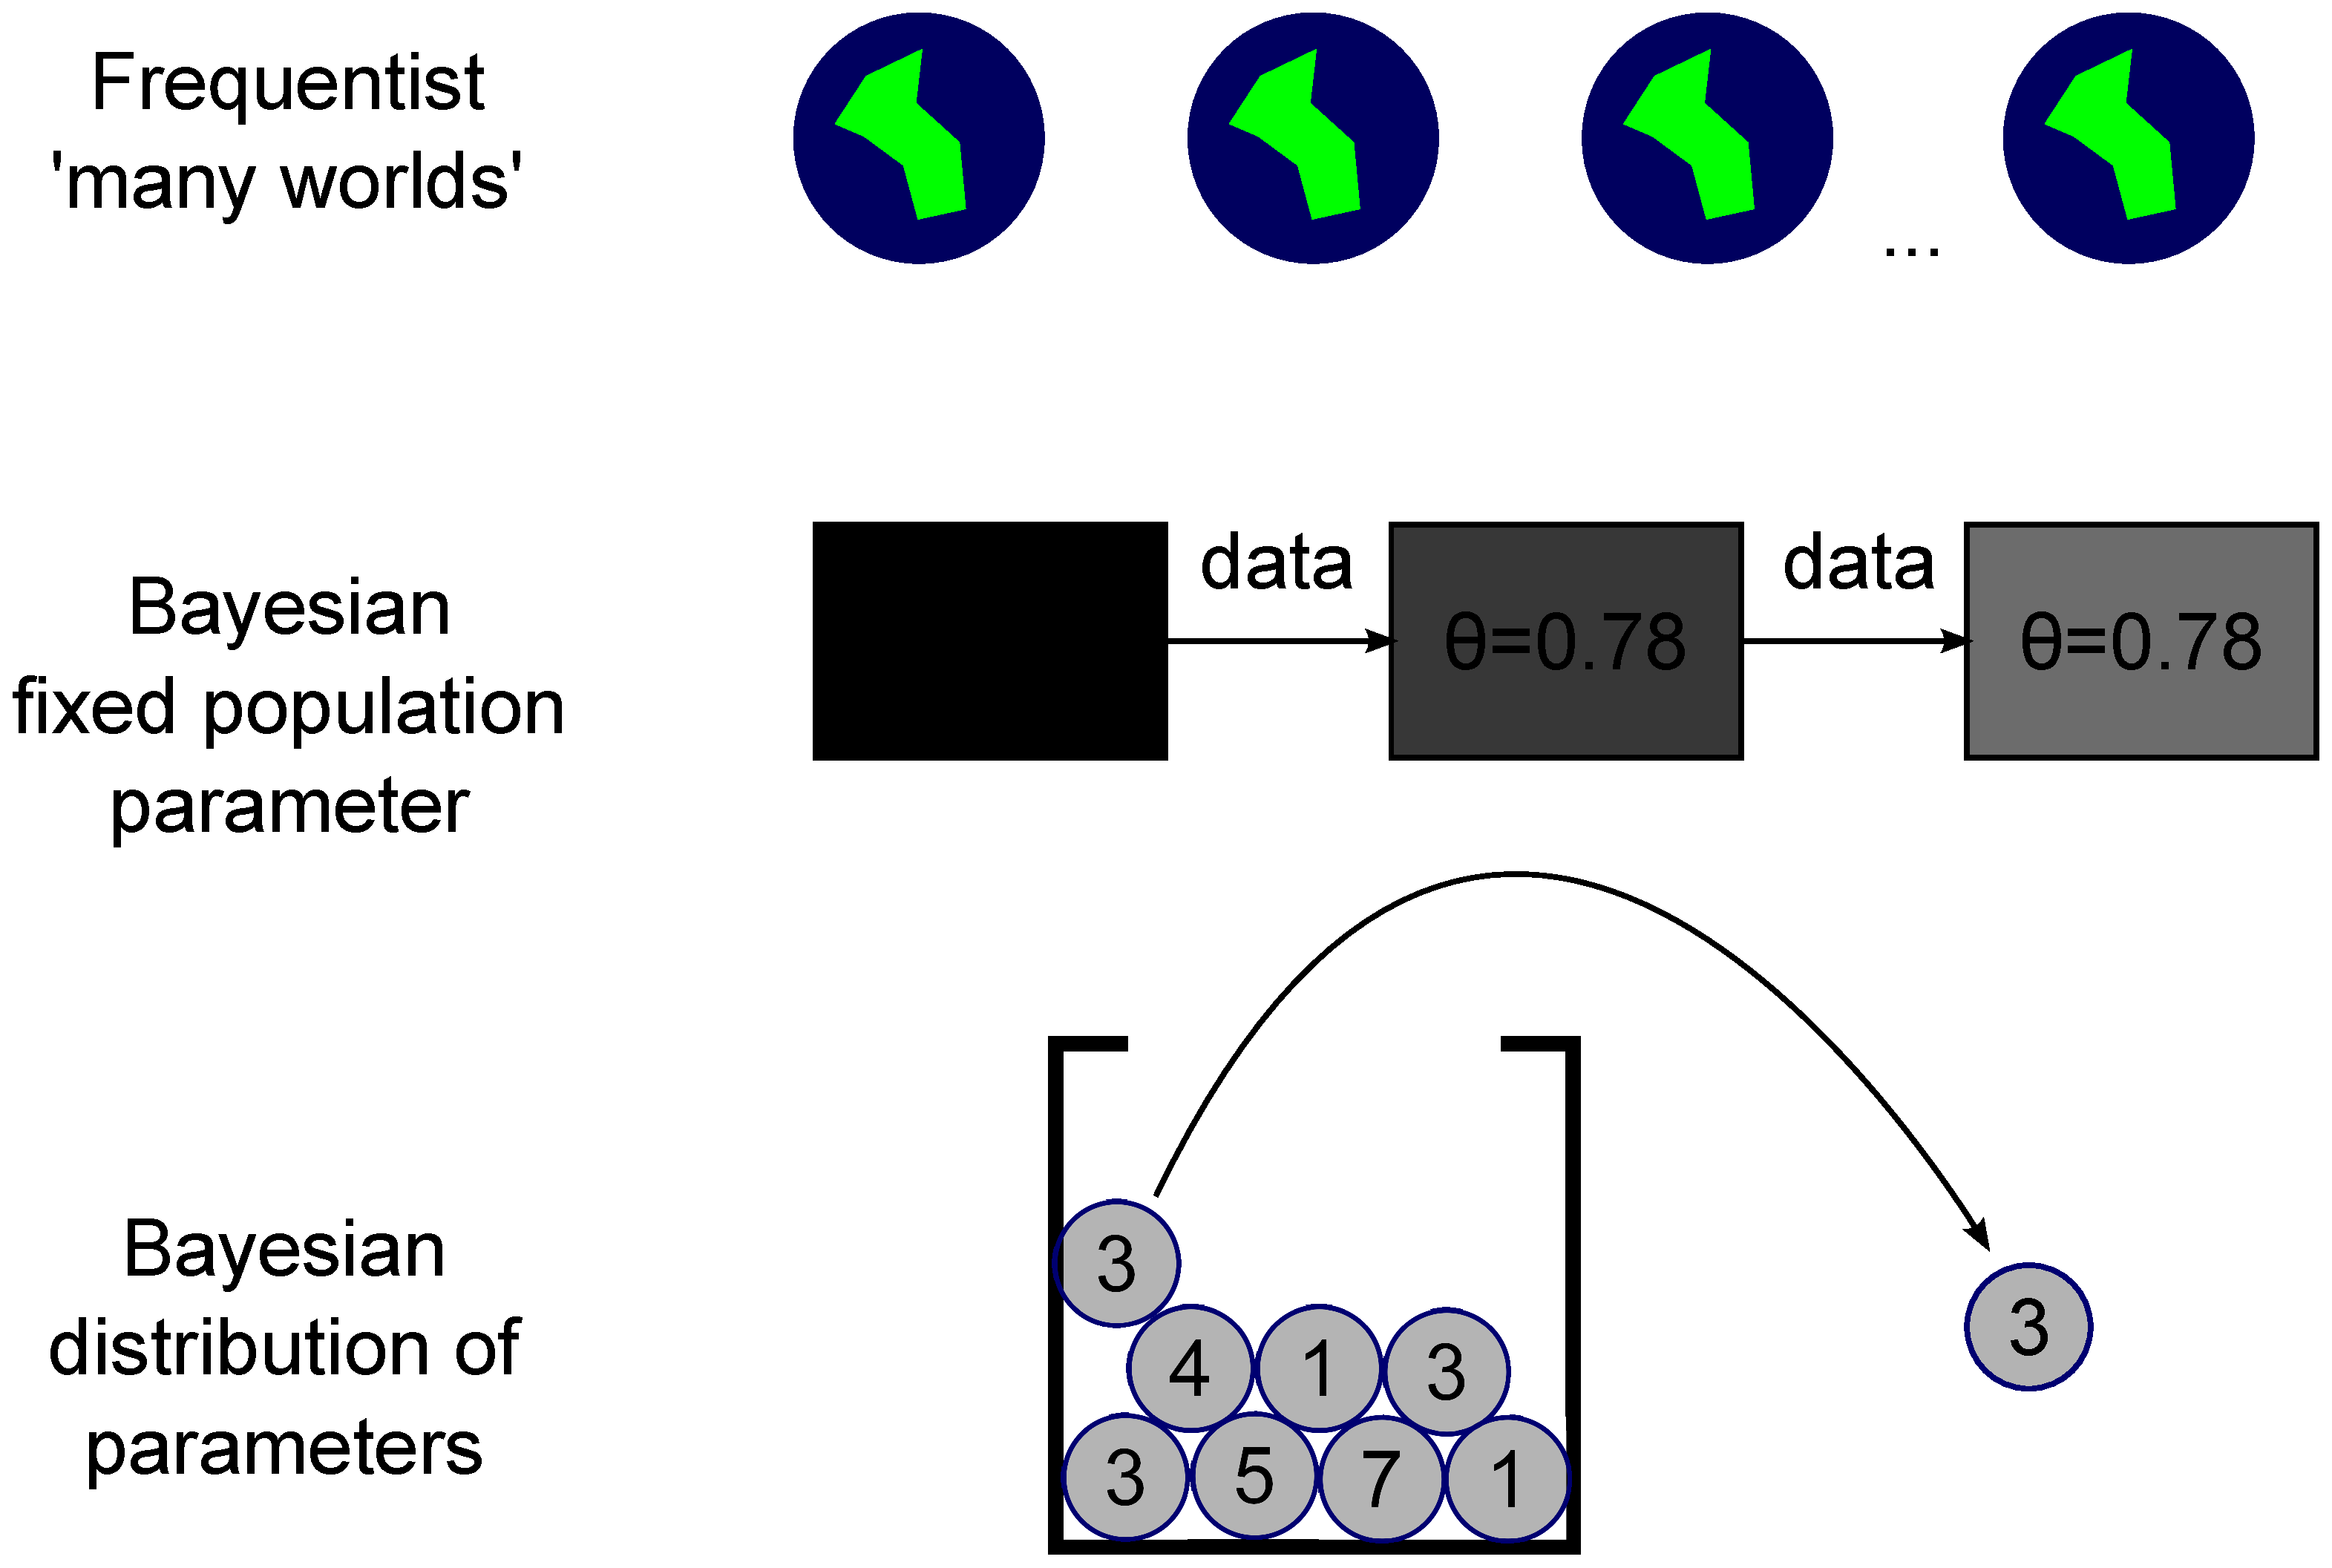
\includegraphics{Posterior_manyWorldsDoParametersExist.eps}}
\caption{The Frequentist and Bayesian perspectives on parameters.}\label{fig:Posterior_manyWorldsDoParametersExist}
\end{figure}

\subsection{Failings of the Frequentist confidence interval}\label{sec:Posterior_classicalConfidenceInterval}
A mainstay of the Frequentist estimation procedure is the \textit{confidence interval}. In empirical research we often see these intervals as stated for a given parameter (where for now we assume that the parameters are unknown and fixed). For example,

\textbf{'From our research, we concluded that the percentage of penguins with red tails, $RT$, has a 95\% confidence interval of $1\%\leq RT \leq 5\%$.'}

This is often incorrectly taken as having an implicit meaning, 'We are 95\% sure that the true percentage of penguins with red tails lies in the range of 1\% to 5\%.' However, what it actually captures is not uncertainty about the parameter in question, but about the interval we calculate. 

In the Frequentist paradigm we imagine that we are taking repeated samples from a population of interest, and for each of the samples, we estimate a confidence interval (see figure \ref{fig:Posterior_classicalConfidenceInterval}). A 95\% confidence interval means that across all of the intervals we calculate, the true value of the parameter will lie in this range 95\% of the time. 

\begin{figure}
\centering
\scalebox{0.4} 
{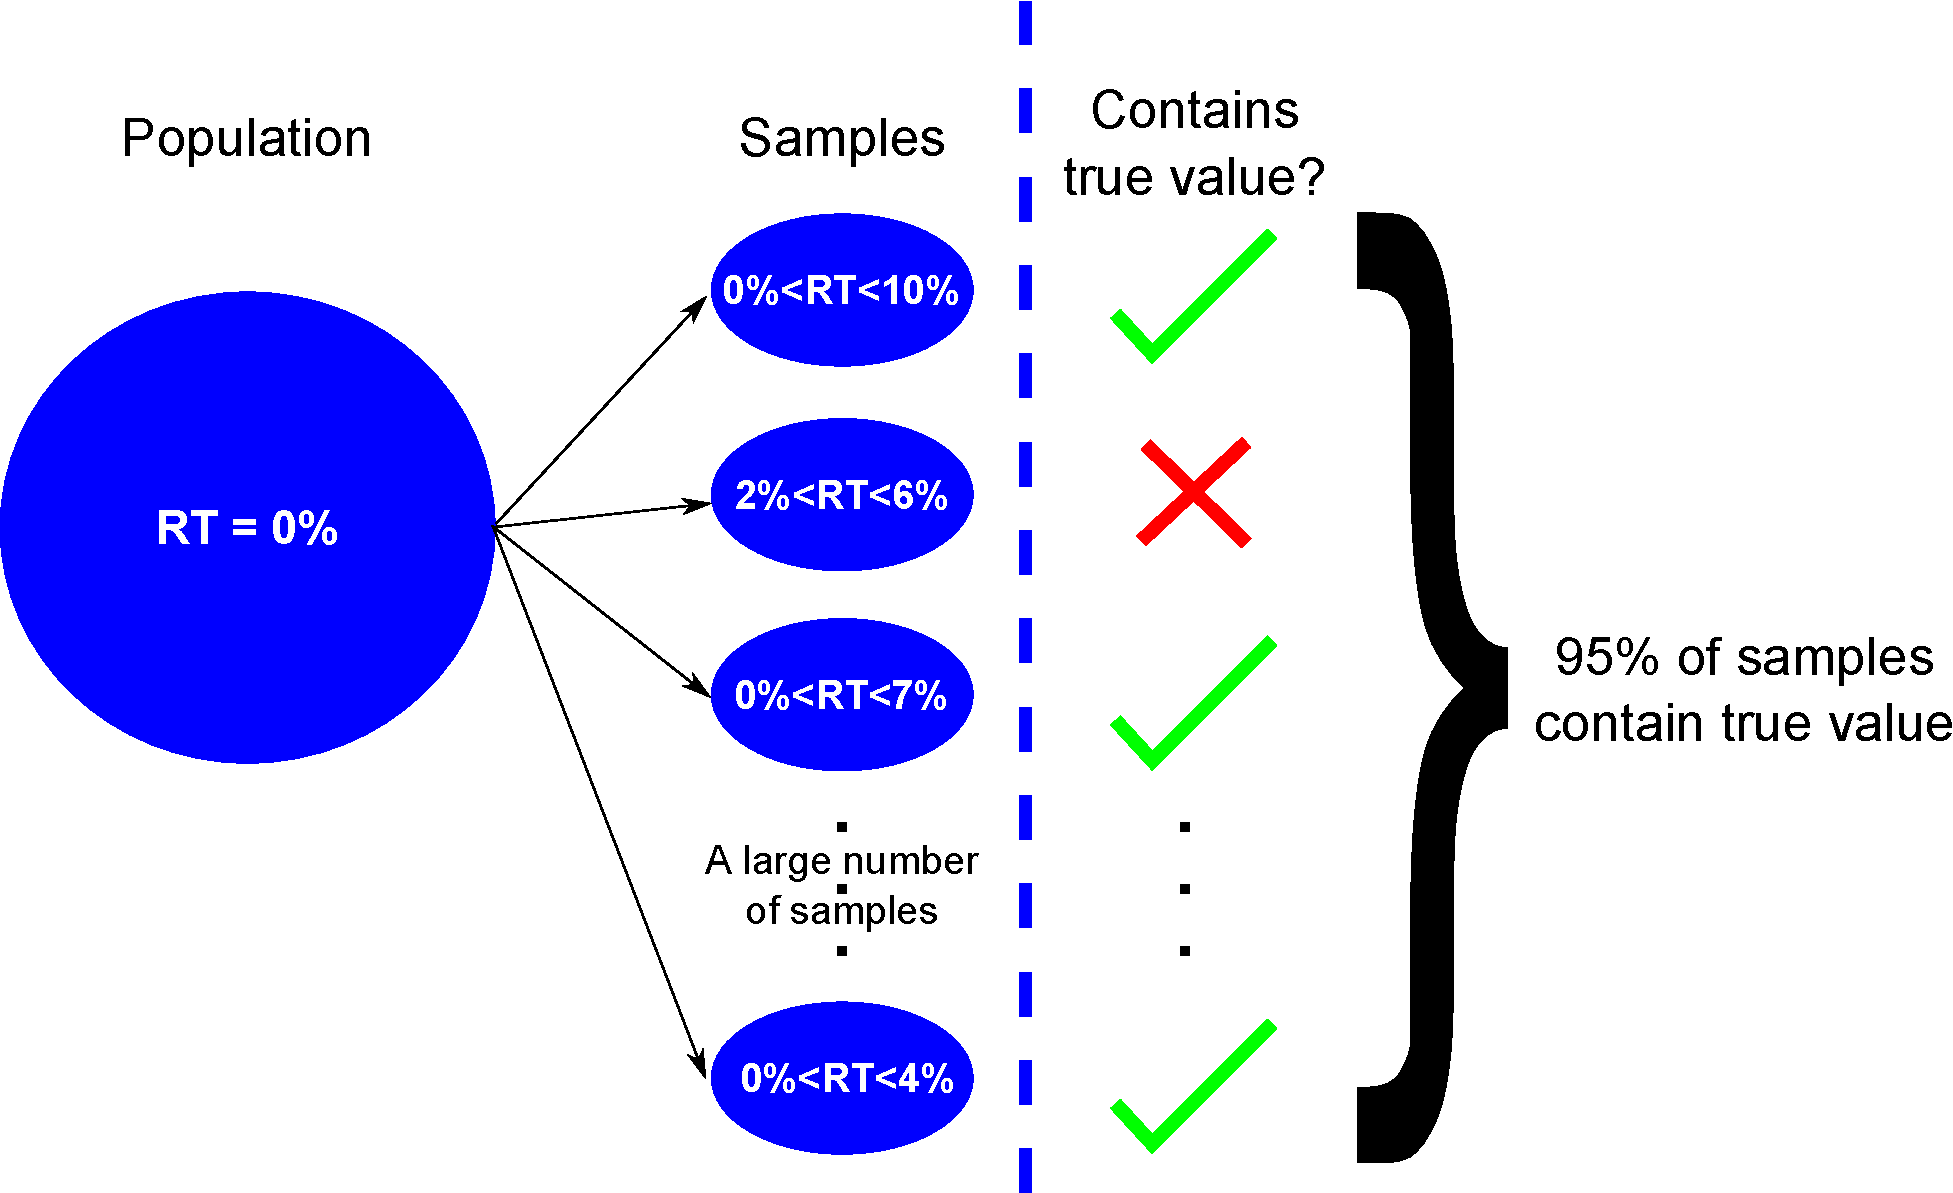
\includegraphics{Posterior_classicalConfidenceInterval.pdf}}
\caption{The classical confidence interval. In each sample, we can calculate a 95\% confidence interval. Across repeated samples from a given population distribution, the classical confidence interval will contain the true parameter value 95\% of time.}\label{fig:Posterior_classicalConfidenceInterval}
\end{figure}

However, what is important to note here is that in reality, we only draw one sample from the population, and we have no way of knowing whether the confidence interval we calculate contains the true parameter value. This means that although 95\% of the time the confidence intervals we calculate will contain the true value of the parameter, and 5\% of confidence intervals will be nonsense!

In general, a confidence interval represents the uncertainty about the interval we obtained, rather than a statement of probability about the parameter of interest. The uncertainty is quantified in terms of all the samples we \textit{could} have taken, not only the one we have in our hands.

\subsection{Credible intervals}
Credible intervals, in contrast to confidence intervals, describe our uncertainty in the location of the parameter values and thus can be interpreted as a probabilistic statement about the parameters. They are a Bayesian concept, that is calculated from the posterior density.

In particular, a 95\% credible region satisfies the condition that 95\% of the posterior density's area lies in this parameter range. The statement below,

\textbf{'From our research, we concluded that the percentage of penguins with red tails, $RT$, has a 95\% credible interval of $0\%\leq RT \leq 4\%$.'}

can be interpreted as, 'From our research, we conclude that there is a 95\% probability that the percentage of penguins with red tails, lies in the range $0\%\leq RT \leq 4\%$'.

In general an arbitrary credible interval of $X$\% can be constructed from the posterior density, by finding a region whose area is equal to $\frac{X}{100}$. 

\begin{figure}
\centering
\scalebox{0.35} 
{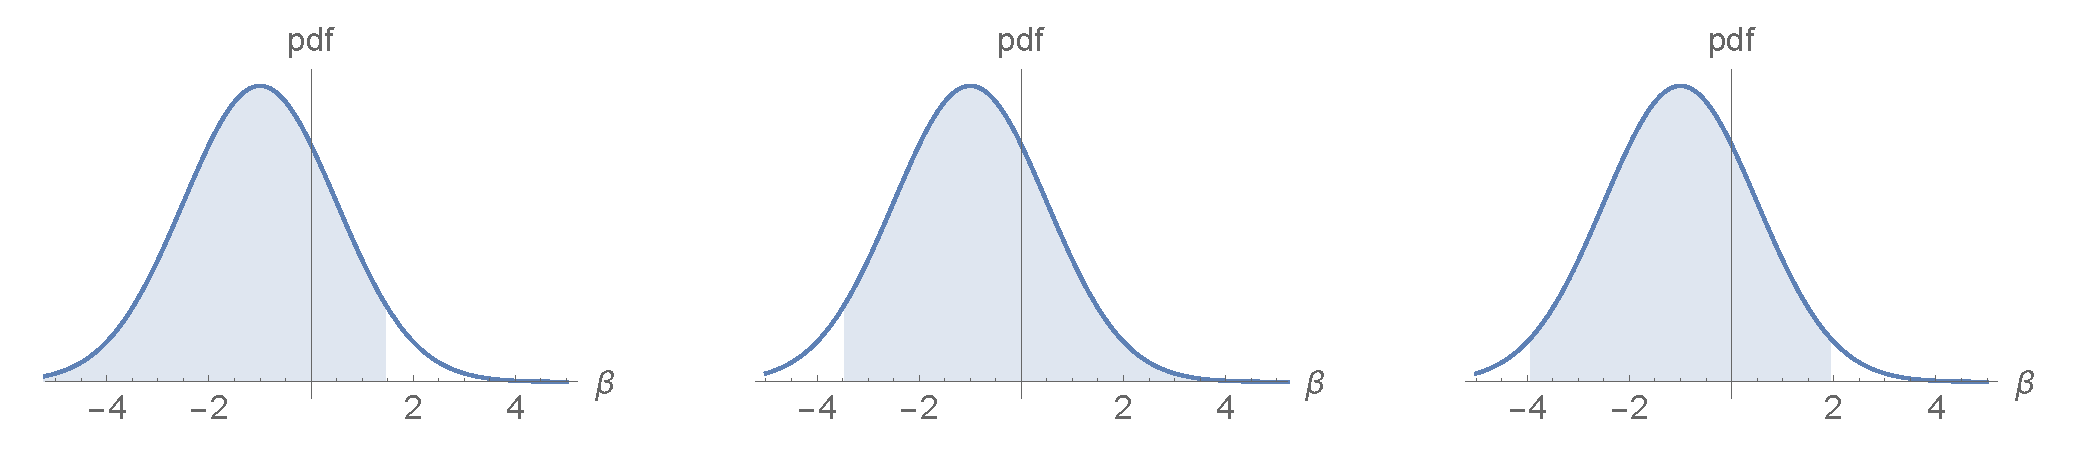
\includegraphics{Posterior_infiniteCredibleIntervals.pdf}}
\caption{Three examples of a 95\% credible interval for the regression parameter $\beta$ of the example described in section \ref{sec:Posterior_parameterUncertainty}.}\label{fig:Posterior_infiniteCredibleIntervals}
\end{figure}

In contrast to the classical confidence interval, a credible interval is more straightforward to understand. It is a probability statement of confidence in the location of a parameter. Also, in contrast to the classical confidence intervals, the uncertainty here refers to our inherent uncertainty in the value of the parameter, rather than an infinity of counterfactual samples.

There are usually an infinite number of regions which satisfy this condition, as figure \ref{fig:Posterior_infiniteCredibleIntervals} indicates for the regression example used in section \ref{sec:Posterior_parameterUncertainty}. All three of the examples shown in figure \ref{fig:Posterior_infiniteCredibleIntervals} satisfy the condition, that given our choice of model and prior, we conclude that there is a 95\% probability that the parameter lies in this range. 

In order to reduce the number of credible intervals down to one, there are 'industry standards' that are followed in most applied research. We introduce two of the most frequently used metrics now.

\subsubsection{Treasure hunting: The central posterior and highest density intervals}\label{sec:Posterior_CPI}\label{sec:Posterior_HDI}
Imagine you (as a pirate) were told by a fortune-teller that treasure of \$1000 is buried somewhere along the seashore of an imagined island. Further, imagine that the mystic has gone to the trouble of using their past experience, and intuition, to arrive at a posterior density for the location of the treasure, along the x-axis seashore, that is shown in figure \ref{fig:Posterior_CPIvsHDI}. The cost to hire a digger to dig up 1km of coastline is \$100.

Suppose you want to find the gold with 95\% certainty, and maximise your profit in doing so\footnote{This is really a Bayesian Decision Theory question, where you are choosing an \textit{action}, which corresponds to an interval; specifying a constant cost function across the domain.}. In order to reach this level of confidence in plundering the gold, you have the choice of the two 95\% credible intervals shown in figure \ref{fig:Posterior_CPIvsHDI}: the left-hand \textit{central posterior interval}, and the right-hand \textit{highest density interval}.

Both of these intervals have the same area, so we are equally likely to find the gold in either. So which one would be best to choose?

The central posterior interval spans a range of $0.25km-9.75km$ along the beach. This would entail a cost of $9.5\times \$100 = \$950$.

The highest density interval by contrast spans two non-contiguous regions, given by $0km-2.5km$ and $7.5km-10km$. Each has a cost of $2.5\times\$100 = \$250$, meaning a total cost of \$500. We pick the right-hand strategy, and cross our fingers!

Intuitively, we should avoid the left-hand central posterior interval since it this involves digging up more coastline which has a very low probability of containing the gold. The right-hand highest density interval avoids this misspent effort by directing our search efforts towards the areas most likely to contain the treasure.

If it was costly to drive a digger a given distance, without digging, then we might change our minds, and favour the contiguous region of the \textit{central posterior interval} over the \textit{highest density interval}. However, in most practical (non-pirate) situations, the most sensible thing to do is to report the highest density interval.

To work out the upper and lower bounds of an X\% central posterior interval, we find the $\frac{X}{2}\%$ and $(100-\frac{X}{2})\%$ quantiles of the posterior distribution. This will result in an interval that is centred on the median parameter value.

To find the X\% highest posterior interval, we find the set of values which contains this percentage of the posterior density area, with the property that the probability density in this set is never lower than outside.

\begin{figure}
\centering
\scalebox{0.35} 
{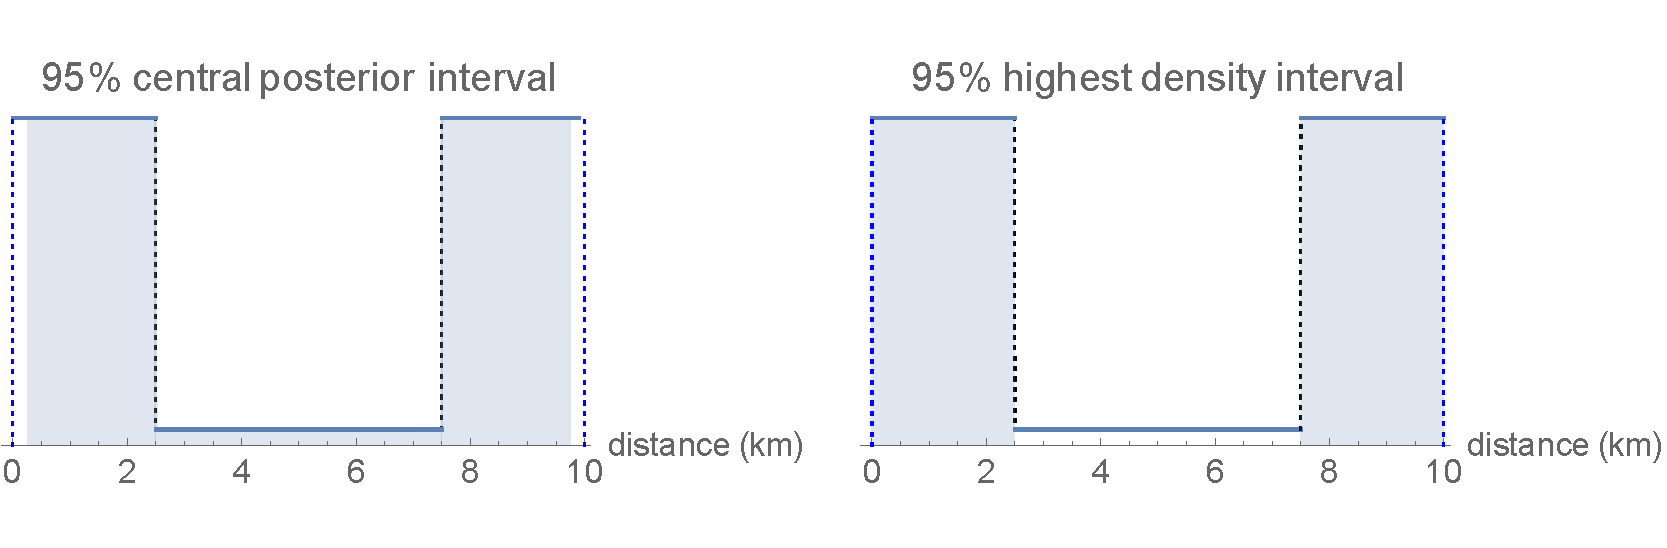
\includegraphics{Posterior_CPIvsHDI.pdf}}
\caption{The posterior probability for treasure being found along the seashore (represented by a linear x-axis).}\label{fig:Posterior_CPIvsHDI}
\end{figure}

For a unimodal, symmetric distribution the central posterior density and highest density intervals will be the same. However, for more complex distributions, this is no longer the case (compare the left and right hand panels of figure \ref{fig:Posterior_CPIvsHDI}).


\subsection{Reconciling the difference between confidence and credible intervals}
It is easy to jump on the bandwagon, and dismiss classical confidence intervals as misleading; favouring the Bayesian alternative definitively. However, in doing so we are somewhat guilty of zealotry. The two concepts really just represent different measures of uncertainty. As we explained in section \ref{sec:Intro_FrequentistsWorld}, Frequentists view data sets as one of an infinity of exactly repeated experiments, and hence design an interval which contains the true value X\% of the time across all these repetitions. The Frequentist confidence interval states uncertainty in terms of the interval itself. By contrast, Bayesians view the data as fixed, and the parameter as coming from an over-arching distribution. They correspondingly calculate an interval where X\% of the parameter's estimated probability mass lies.

The main problem with the classical confidence interval is more that it is often interpreted \textit{incorrectly}, as a \textit{credible} interval. It is not necessarily a problem with the concept itself (although \textit{p values} and hence confidence intervals can be shown to violate the likelihood principle\footnote{Experiments yielding identical likelihoods should yield the same inferences.}). It just depends on your personal preference, and situation, as to which you find more useful.

The following (slightly silly) example hopefully makes this difference of viewpoint clearer. 

\subsubsection{The interval ENIGMA}
Suppose that at the outbreak of war, you are employed as a code breaker in hut 8 at Bletchley Park. By monitoring enemy communications we are able to identify the \textit{source} of the message, although not its \textit{contents}. The source of the message is either submarine, boat, tank or aircraft. The content of the messages is details of the next domestic target of the enemy, and can either be dams, ports, towns or airfields.

Fortunately, previous code-breakers have managed to decode a significant proportion of messages, and have tallied up the proportions of communications from each source, which resulted in a particular attack destination (see figure \ref{tab:Posterior_confidenceIntervalHistoric}). We also know from experience that the proportion of attacks on each destination are roughly similar.


\begin{table}[htbp]
  \centering
    \begin{tabular}{ccccc}
    \toprule
          & \multicolumn{4}{c}{\textbf{Attack destination}} \\
    \midrule
    \textbf{Communication method} & Dam & Port & Town & Airfield \\
    Submarine & 73\%  & 50\%  & 50\%  & 13\% \\
    Boat  & 9\%   & 25\%  & 25\%  & 16\% \\
    Tank  & 0\%   & 25\%  & 25\%  & 66\% \\
    Aircraft & 18\%   & 0\%  & 0\%   & 5\% \\
    \bottomrule
    Total & 100\% & 100\% & 100\% & 100\% \\
    \end{tabular}%
  \caption{Historical communication frequencies resulting in an attack on a given location.}\label{tab:Posterior_confidenceIntervalHistoric}
\end{table}%

Our job is to predict the next attack destination \textit{given} that we have received the mode of communication used. Since there is uncertainty regarding the attack destination, we shall be making confidence intervals which consist of groups of these entities. We are told to use the most narrow\footnote{We suppose there is a cost to readying a destination against attack.} intervals of width greater than or equal to 75\% in all cases.

From this historical evidence we first put the data into a 'statistics-machine', turning the knob that says 'classical confidence intervals'. The result are the confidence intervals shown in table \ref{tab:Posterior_confidenceIntervalClassical}. Note that in all cases the sum of the interval values contained in each column exceeds the threshold. So, for every attack destination, our intervals ensure that the true attack destination lies within the specified sets at least 75\% of the time.

\begin{table}[htbp]
  \centering
    \begin{tabular}{cccccc}
    \toprule
          & \multicolumn{4}{c}{\textbf{Attack destination}} & \multicolumn{1}{c}{\textbf{}} \\
    \midrule
    \textbf{Communications method} & Dam & Port & Town & Airfield   & \textbf{Credibility} \\
    Submarine & \color{red}{$[$73\%}  & \color{red}{50\%}  & \color{red}{50\%$]$}  & 13\%  & \textbf{93\%} \\
    Boat  & \color{red}{$[$9\%}   & \color{red}{25\%}  & \color{red}{25\%}  & \color{red}{16\%$]$}  & \textbf{100\%} \\
    Tank  & 0\%   & 25\%  & 25\%  & \color{red}{$[$66\%$]$}  & \textbf{57\%} \\
    Aircraft & 18\%   & 0\%  & 0\%   & 5\%   & \textbf{0\%} \\
    \bottomrule
    \textbf{Coverage} & \textbf{82\%}  & \textbf{75\%}  & \textbf{75\%}  & \textbf{82\%} &  \\
    \end{tabular}%
  \caption{Classical confidence intervals calculated from data shown in table \ref{tab:Posterior_confidenceIntervalHistoric}. Confidence intervals greater than or equal to 75\% are indicated in red, surrounded by parentheses.}\label{tab:Posterior_confidenceIntervalClassical}%
\end{table}%

We next turn the dial to 'Bayesian credible intervals', and obtain the results shown in table \ref{tab:Posterior_confidenceIntervalBayesian} (see section \ref{sec:Posterior_appendixConfidenceInterval} for a full explanation). In this case, we are implicitly assuming that the choice of destination is a random variable, and that the enemy chooses amongst them uniformly\footnote{Which isn't unreasonable given that we know from experience that the enemy attacks each of these locations in similar proportions.}. In this case, since the sum of interval values in each row exceeds 75\%, we have credible intervals. With these intervals, for each mode of communication, we will ensure that the true attack destination is contained within these destinations at least 75\% of the time.

\begin{table}[htbp]
  \centering
    \begin{tabular}{cccccc}
    \toprule
          & \multicolumn{4}{c}{\textbf{Attack destination}} &  \\
    \midrule
    \textbf{Communication method} & Dam & Port & Town & Airfield   & \textbf{Credibility} \\
    Submarine & \color{red}{$[$73\%}  & \color{red}{50\%}  & \color{red}{50\%$]$}  & 13\%  & \textbf{93}\% \\
    Boat  & \color{red}{$[$9\%}   & \color{red}{25\%}  & \color{red}{25\%$]$}  & 16\%  & \textbf{79}\% \\
    Tank  & 0\%   & 25\%  & \color{red}{$[$25\%}  & \color{red}{66\%$]$}  & \textbf{78}\% \\
    Aircraft & \color{red}{$[$18\%$]$}   & 0\%  & 0\%   & 5\%   &\textbf{78\%} \\
    \bottomrule
    \textbf{Coverage} & \textbf{100\%}  & \textbf{75\%} &\textbf{ 100\%}  & \textbf{66\%}  &  \\
    \end{tabular}%
   \caption{Bayesian credible intervals calculated from data shown in table \ref{tab:Posterior_confidenceIntervalHistoric}. Credible intervals greater than or equal to 75\% are indicated in red, surrounded by parentheses. Note: 'credibility' is calculated by dividing the sum of interval values in each row by the row's total (see section \ref{sec:Posterior_appendixConfidenceInterval} for a full explanation.)}\label{tab:Posterior_confidenceIntervalBayesian}%
\end{table}%

The difference between these two measures is subtle. In fact, as is often the case, the intervals are actually similar, and overlap considerably. But which should we choose? Using the classical confidence intervals, we are assured that whatever destination the enemy chooses, our interval will contain the true attack destination at least 75\% of the time. A Bayesian would criticise the confidence interval for the case of the \textit{Aircraft} communication method, since this is the empty interval! This clearly is nonsensical, since we know that one of the locations is about to be attacked. This error could be particularly costly if attacks coordinated via Aircraft are particularly costly. A Frequentist would argue that since, \textit{at most}, Aircraft communications happen 18\% of the time (for dams), this isn't something to worry about.

A Bayesian would also criticise a classical confidence interval, since for a given communication mode, what is the use in worrying about all the other communication modes? We aren't uncertain about the communication mode!

A Frequentist would argue that for attacks on airfields, the Bayesian confidence intervals only correctly predict this as the attack destination 66\% of the time. Again, if these types of attack are particularly costly, then this interval might not be ideal\footnote{If we were to assign costs to each of these attack events, then we could work out optimal intervals, although this is the realm of Bayesian Decision Theory; not covered in this text.}. A Bayesian would argue that, assuming a uniform prior, this type of attack only happens 25\% of the time, and so is not something to worry about. Further, for every mode of communication, our credible intervals are guaranteed to never be nonsense, in contrast to the classical confidence interval.

\section{Point parameter estimates}
Whilst it is beneficial to estimate the entire posterior distribution for a particular parameter, we are often required to give point estimates. This is sometimes for direct comparison with Frequentist approaches, but more often it is to allow people not versed in Bayesian statistics to make decisions\footnote{The correct process in order to make decisions using posterior distributions is through decision theory, not covered in this text. A good review of this field is provided in \cite{robert2007bayesian}.}. We want to reiterate, that we are \textit{not} advocating these estimators\footnote{Rules that take an input, and produce estimates.} as a replacement to providing the entire posterior distribution; only that they are useful summaries which supplement an analysis.

There are three main approaches here, although we argue that only two out of the three should be used. These estimators can be summarised as:

\begin{itemize}
\item The posterior mean.
\item The posterior median.
\item The maximum a posteriori estimator (MAP).
\end{itemize}

The posterior mean is simply defined for a univariate-continuous example as:

\begin{equation}
\mathrm{E}[\theta|data] = \int\limits_{\Theta} \theta p(\theta|data)\mathrm{d}\theta
\end{equation}

For the discrete case, we replace the integrals above with summations (see section \ref{sec:Probability_meanVariance}). 

The posterior median is the point of a posterior distribution to which 50\% of its area (the probability), lies to its left. The MAP estimator is simply the highest point in the posterior (see figure \ref{fig:Posterior_meanMedianMAP}).

Whilst each of these three estimators can be optimal for a given loss function\footnote{A decision theoretic concept, again.}, we believe that there is a clear hierarchy of these estimators. At the top of the hierarchy - denoting our preferred estimator - we have the posterior mean. This is our favourite for two reasons: firstly, it normally yields \textit{sensible} estimates, which are fairly representative of the central position of the posterior distribution; secondly, and more mathematically, this estimator makes sense from a measure-theoretic perspective, since the quantity of interest is a probability not a density. The density depends on the particular parameterisation that we choose, the probability should not. Don't worry about this last point too much, we just wanted to mention it for completeness. Next down the hierarchy we have the posterior median. This is usually pretty close to the mean (see figure \ref{fig:Posterior_meanMedianMAP}), and is often indicative of our posterior distribution. It is sometimes preferable to use a median if the mean is heavily-skewed by a slowly-changing density, although the choice between the two estimators depends on circumstance.

At the bottom of the hierarchy, we have the MAP estimator. Proponents argue that the simplicity of this estimator is a benefit. Since it maximises the posterior, across values of the parameter, we do not actually need to calculate the tricky denominator (see chapter \ref{chap:denominator}), as this is independent of the parameter. This means that it is often feasible to find the MAP estimator exactly, even if this is not possible for the other two measures. However, its simplicity is misleading. Importantly, the mode of a distribution often lies away from the majority of the probability distribution's area, and is hence not a particularly indicative central measure of the posterior. Secondly, and mathematically, this estimator does not make sense because it relies on the density, which depends on the particular parameterisation in question.

The bottom line is that one should not use the MAP estimator unless you have a \textit{very} good reason for doing so. 

\begin{figure}
\centering
\scalebox{0.4} 
{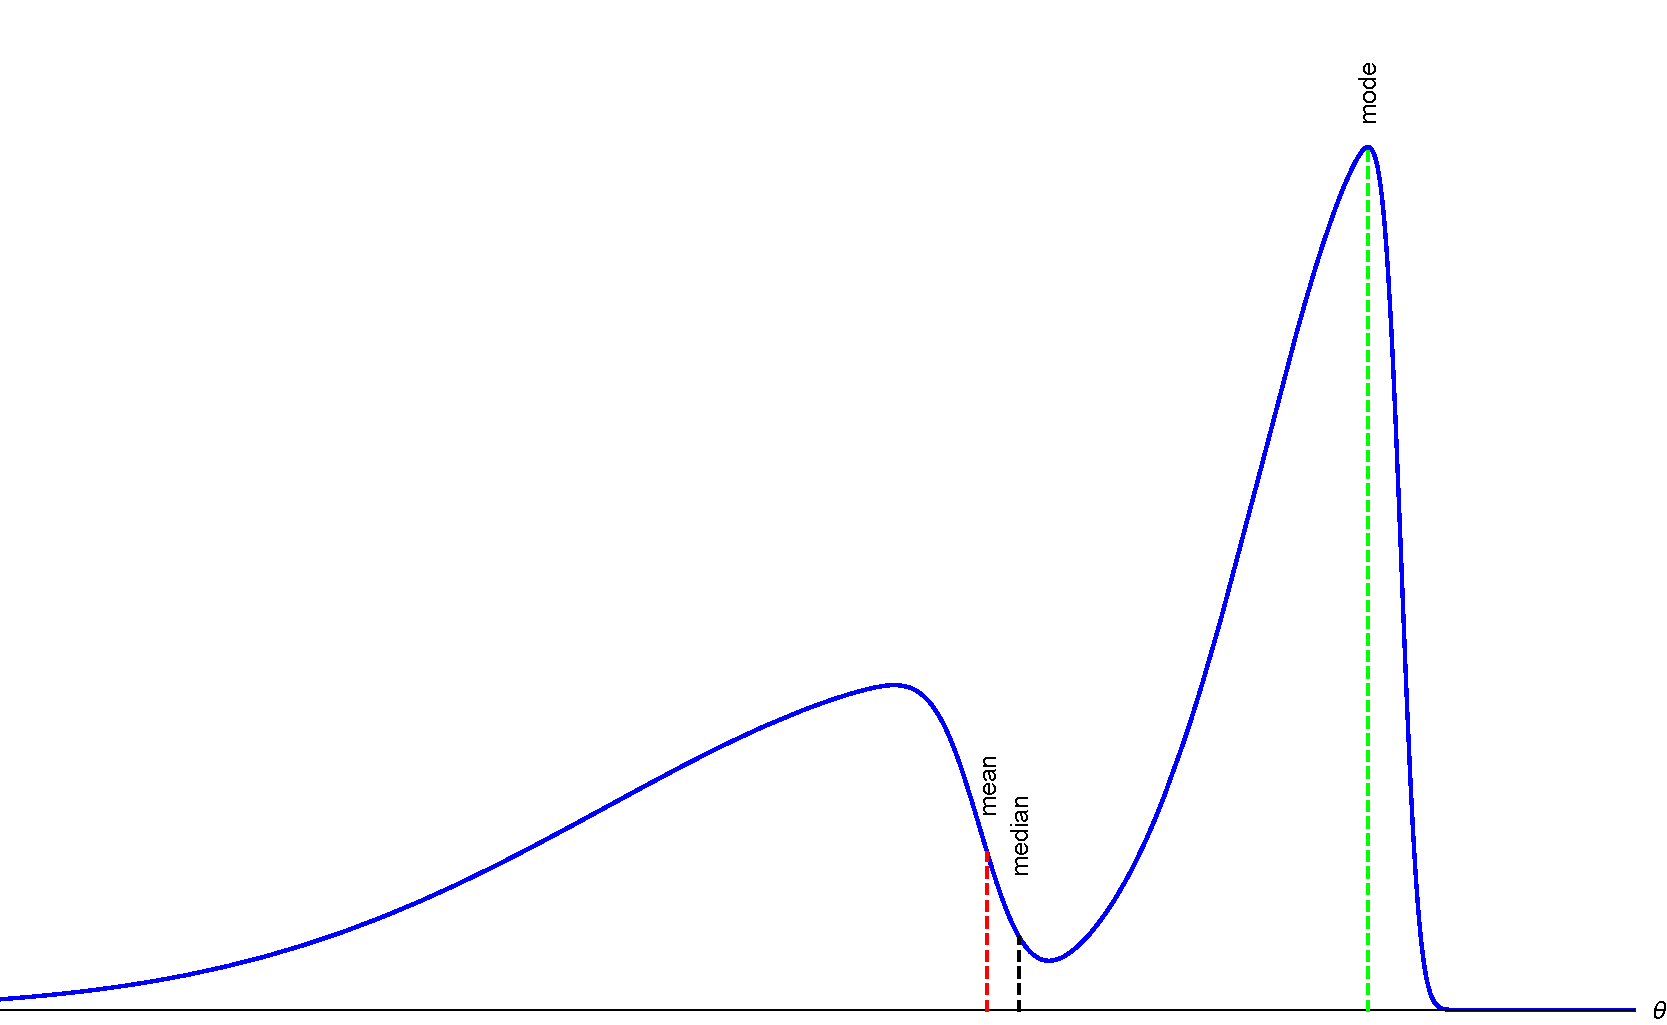
\includegraphics{Posterior_meanMedianMAP.pdf}}
\caption{The mean, median and mode for a skewed, multi-modal distribution.}\label{fig:Posterior_meanMedianMAP}
\end{figure}


\section{Prediction using predictive distributions}\label{sec:Posterior_predictiveDistributions}
Parameters of a statistical distribution are typically only of interest insomuch as they influence \textit{real variables}, for which we collected data in the first place. Be it income levels, disease cases, or electoral votes; the data is what drove us to conduct a statistical analysis. As such, it is frequently useful to compare models (which may have very different statistical formulations) using this common currency, of \textit{data}.

Before we have run our model, we only have our prior views of the likely values of parameters. It is often informative to convert from the currency of \textit{parameters}, to that of \textit{data}, in order to evaluate the tangible implications of the chosen priors\footnote{See chapter \ref{chap:Prior} for a much more in-detail discussion.}.

Also, after we have fed our priors and likelihoods into the Bayesian formula, we are outputted with the posterior distribution for our parameters of interest. Fortunately, both of these are simple, due to the manipulable nature of probabilities.

\subsection{Example: number of Republican voters within a sample}
You find yourself working for a polling organisation, ahead of the next US Presidential election. Your job is to try to predict, out of a sample of 100 people, what will be the number voting for the Republican party. Based on previous work, you expect that the proportion of Republican voters in a sample, $\theta$, can be represented by the prior distribution, $p(\theta)$, shown in the top-left of figure \ref{fig:Posterior_priorPosteriorPredictiveVoting}. To evaluate the implications of this prior, we would like to know what this means in terms of number, $x$, of people out of our sample of 100, who will vote for the Republicans; in other words, the \textit{prior predictive distribution}. Fortunately, we can obtain this by manipulating probabilities, although we need to specify a likelihood function, $p(x|theta)$; in this case we pick a binomial distribution\footnote{The relevance and nice fit of this distribution is explained in full in chapter \ref{chap:Likelihoods}, so do not worry if you don't follow its use here.}. The prior predictive distribution here is essentially the marginal distribution of $x$, which we know from section \ref{sec:Probability_marginal} can be obtained by integrating\footnote{Since the parameter is continuous here.} out the dependence of the parameter $\theta$ from the joint distribution $p(x,\theta)$:

\begin{align}\label{eq:Posterior_priorPredictiveVoting}
p(x) &= \int\limits_{0}^{1} p(x,\theta) \mathrm{d}\theta\\
&= \int\limits_{0}^{1} p(x|\theta) p(\theta) \mathrm{d}\theta
\end{align}

\begin{figure}
\centering
\scalebox{0.4} 
{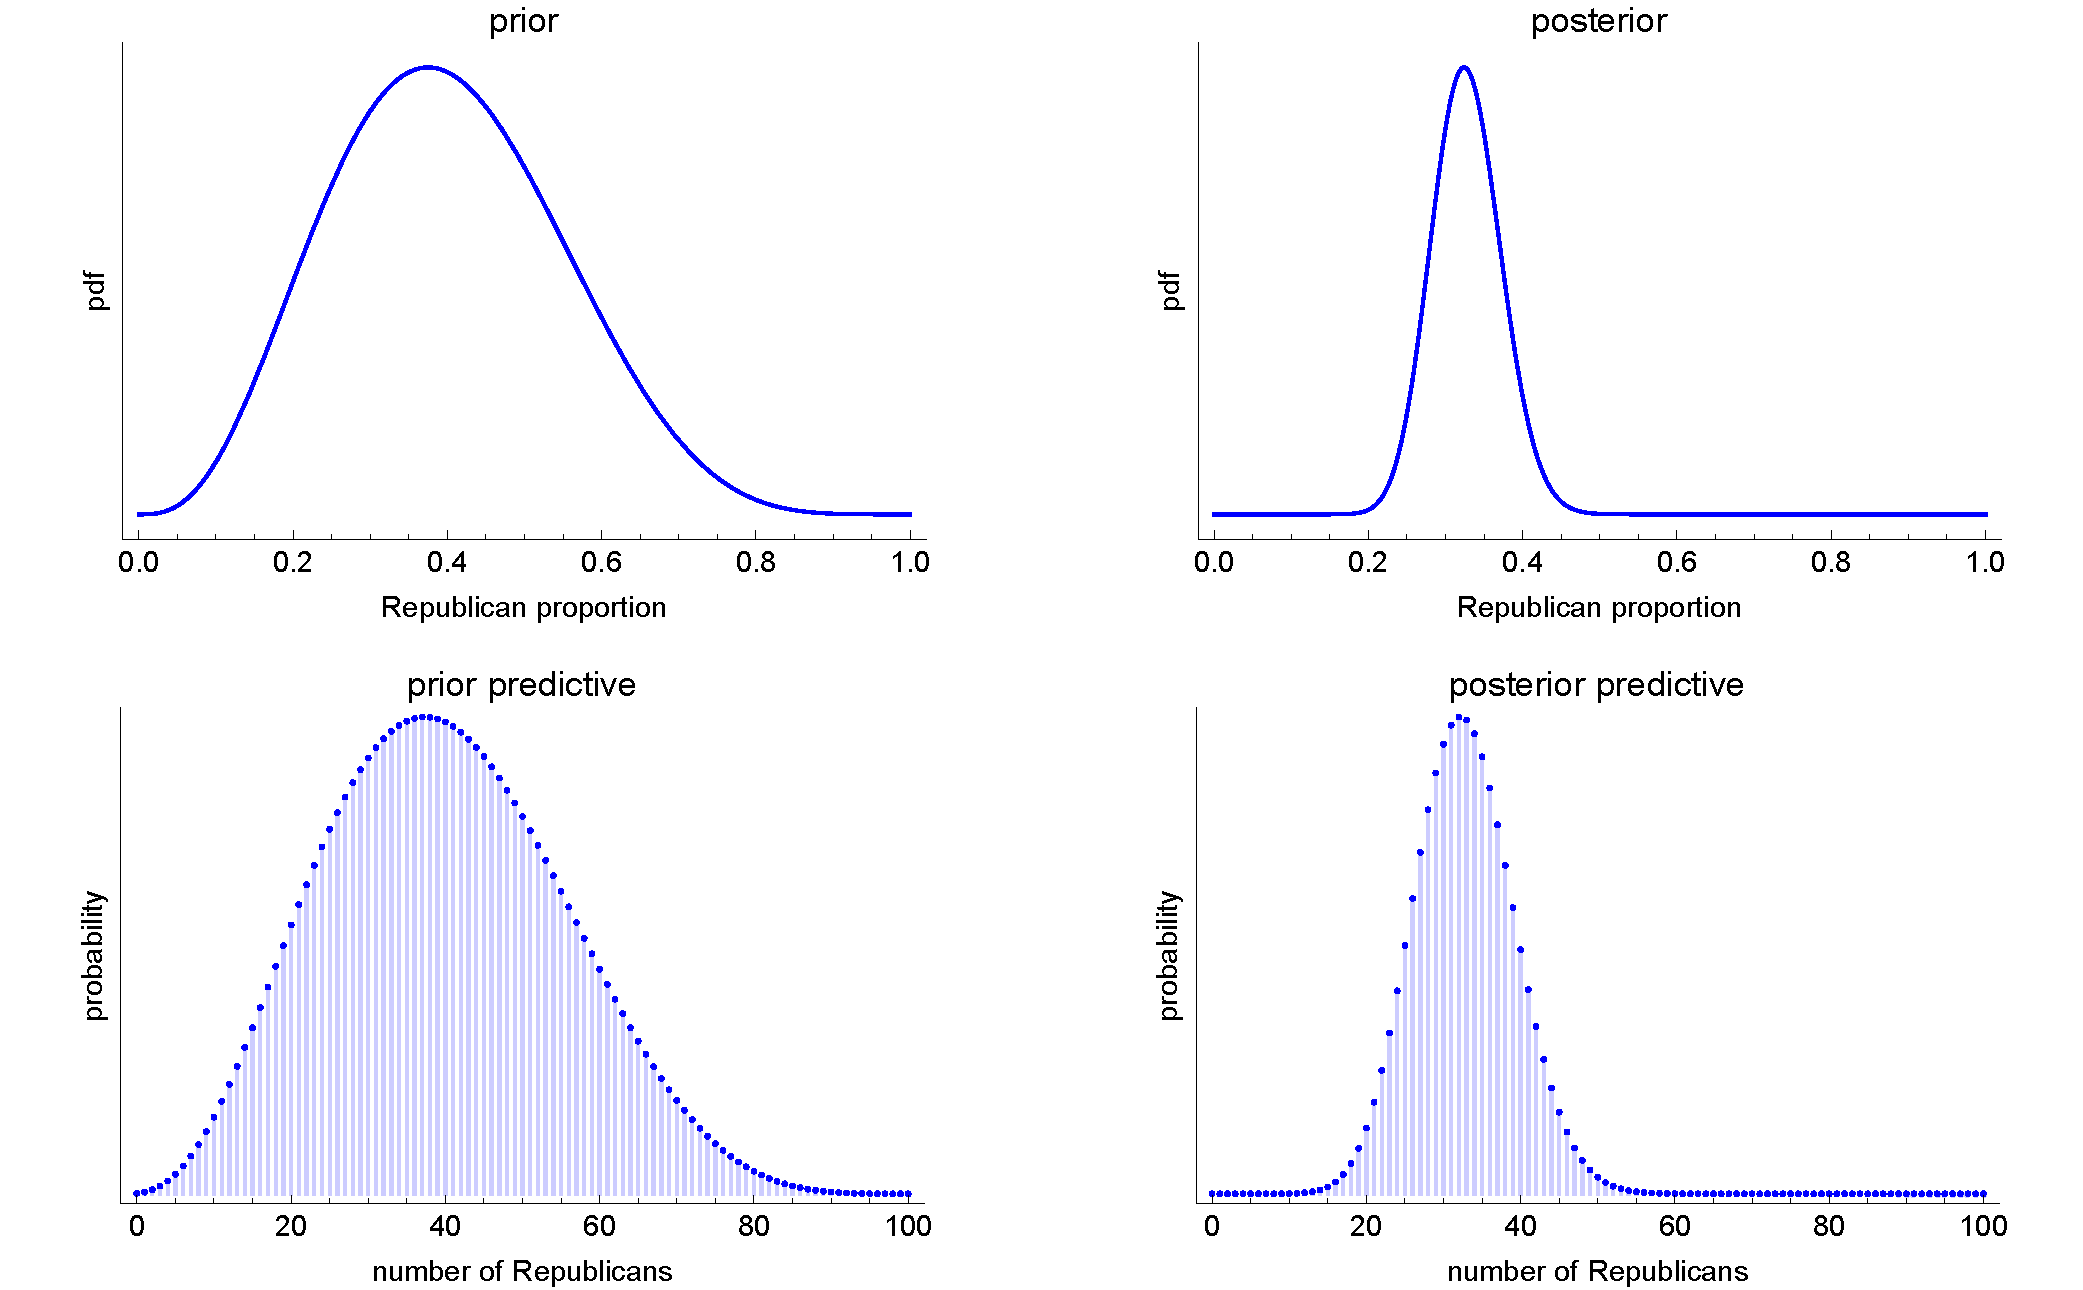
\includegraphics{Posterior_priorPosteriorPredictiveVoting.pdf}}
\caption{Top-left: the prior proportion of people voting for the Republican party in a sample of 100, resulting in the prior predictive distribution shown in the bottom-left. Top-right: the posterior proportion of people voting Republican, resulting the bottom-right posterior predictive distribution.}\label{fig:Posterior_priorPosteriorPredictiveVoting}
\end{figure}


where to get to the second line from the first, we have used the conditional law of probability (\ref{eq:Probability_conditionalProbability}), to decompose the joint distribution into a conditional and prior. Notice that the prior predictive distribution is essentially a sum of the probability of $x$ conditional on $\theta$, weighted by our prior probability to that proportion, $\theta$, voting Republican. In this case, this results in the intuitive result, where the prior density and the prior predictive distribution\footnote{This is predictably called a Beta-binomial distribution, since it is made from combining a Beta prior, with a Binomial likelihood. Don't worry though, we will discuss this in detail in chapter \ref{chap:conjugate}.} exactly line up (albeit on different scales).

After our first sample of 100 people from that particular location, we find that 32 of them would vote Republican. We use this data to calculate our likelihood, then combine this with our prior via Bayes' rule; obtaining the posterior density shown in the top-right of figure \ref{fig:Posterior_priorPosteriorPredictiveVoting}. Our job is now to estimate the number of people who will vote republican in a new sample, of the same size. Ideally, we would like to have a probability distribution to describe all the possible outcomes. This distribution is known as the \textit{posterior predictive distribution}, because it is that which we would predict \textit{after} obtaining our data sample. It is written as $p(x'|x)$ where $x'$ represents the number of people voting Republican in the new sample, and $x$ is the number voting Republicans in the previous sample ($x=32$). We can use a method exactly analogous to that which we used previously, by integrating out $\theta$ dependence of the joint distribution of $x'$ and $\theta$, although now we have to condition on $x$:

\begin{align}\label{eq:Posterior_posteriorPredictiveVoting}
p(x'|x) &= \int\limits_{0}^{1} p(x',\theta|x) \mathrm{d}\theta\\
&= \int\limits_{0}^{1} p(x'|\theta,x) p(\theta|x) \mathrm{d}\theta\\
&= \int\limits_{0}^{1} p(x'|\theta) p(\theta|x) \mathrm{d}\theta
\end{align}

Note that to get from the second line from the first, we have used the same conditional probability law  (\ref{eq:Probability_conditionalProbability}), as we used for the prior predictive case. The only difference here is that we are additionally conditioning on $x$. To get from the second to the third line we have used a typical assumption, which is that once $\theta$ is known, the likelihood for our new sample does not depend on the previous data $x$. Another way to think about this is that all the information in $x$ has been used to estimate $\theta$; meaning that it does not confer any further information which is helpful for predicting $x'$. Again, we note in figure \ref{fig:Posterior_priorPosteriorPredictiveVoting} how the posterior predictive distribution lines up exactly with the posterior distribution of $\theta$. This makes intuitive sense, since if we predict the most likely \textit{proportion} to vote Republicans is 0.32, we should expect that this will translate into the most likely \textit{number} of $0.32\times 100=32$, in a sample of 100.

\subsection{Example: interest rate hedging}
Suppose that you work as an analyst in an investment bank, focussing on predicting the actions of the central bank, so that your investments can be sufficiently hedged. The return of a certain investment, $x$, is probabilistically dictated by the rate of interest, and is also discrete; following a poisson distribution with rate parameter given by the chosen rate. Imagine that the current rate of interest is 1\%, and the bank sets rates at 0.5\% intervals; yielding a discrete distribution of possible values: $i\in[0.5\%, 1.0\%, 1.5\%, 2.0\%, 2.5\%,3.0\% ]$; resulting in the likelihood\footnote{Do not worry about the use of likelihoods here, as we shall explain this concept fully in chapter \ref{chap:Likelihoods}.} shown in figure \ref{fig:Posterior_likelihoodInterestRate}.

\begin{figure}
\centering
\scalebox{0.65} 
{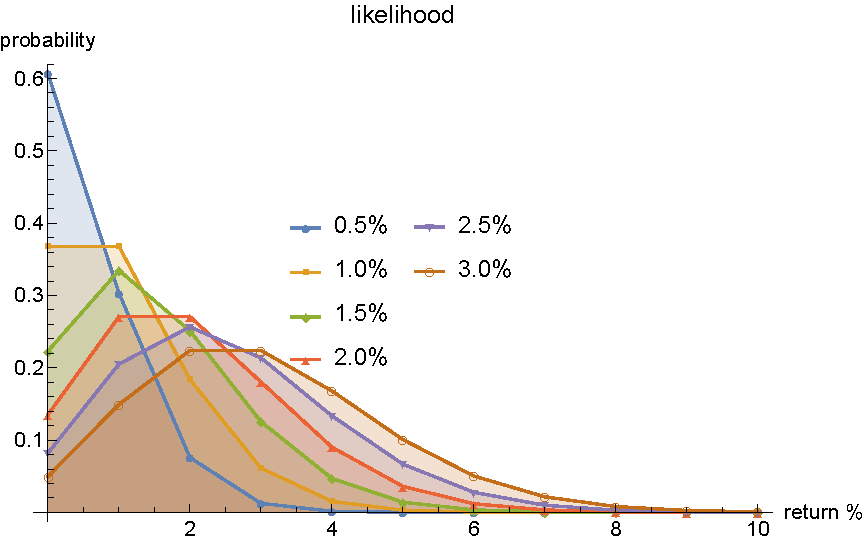
\includegraphics{Posterior_likelihoodInterestRate.pdf}}
\caption{The likelihood of different rates of return across different central bank interest rates.}\label{fig:Posterior_likelihoodInterestRate}
\end{figure}

The pre-data-analysis probabilities that your in-house economist gives to each different central bank rate are shown in figure \ref{fig:Posterior_priorPosteriorInterestRate}. After combining these expert views with a probabilistic model, which looks at historical rate decisions, this results in the posterior distribution of probabilities shown in figure \ref{fig:Posterior_priorPosteriorInterestRate}; illustrating considerable discordance between the data's view, and those of your economist\footnote{This might indicate that your economist doesn't know his head from his hands, \textit{or} he believes there is reason to suggest that this rate decision will be different to those historically.}.

\begin{figure}
\centering
\scalebox{0.45} 
{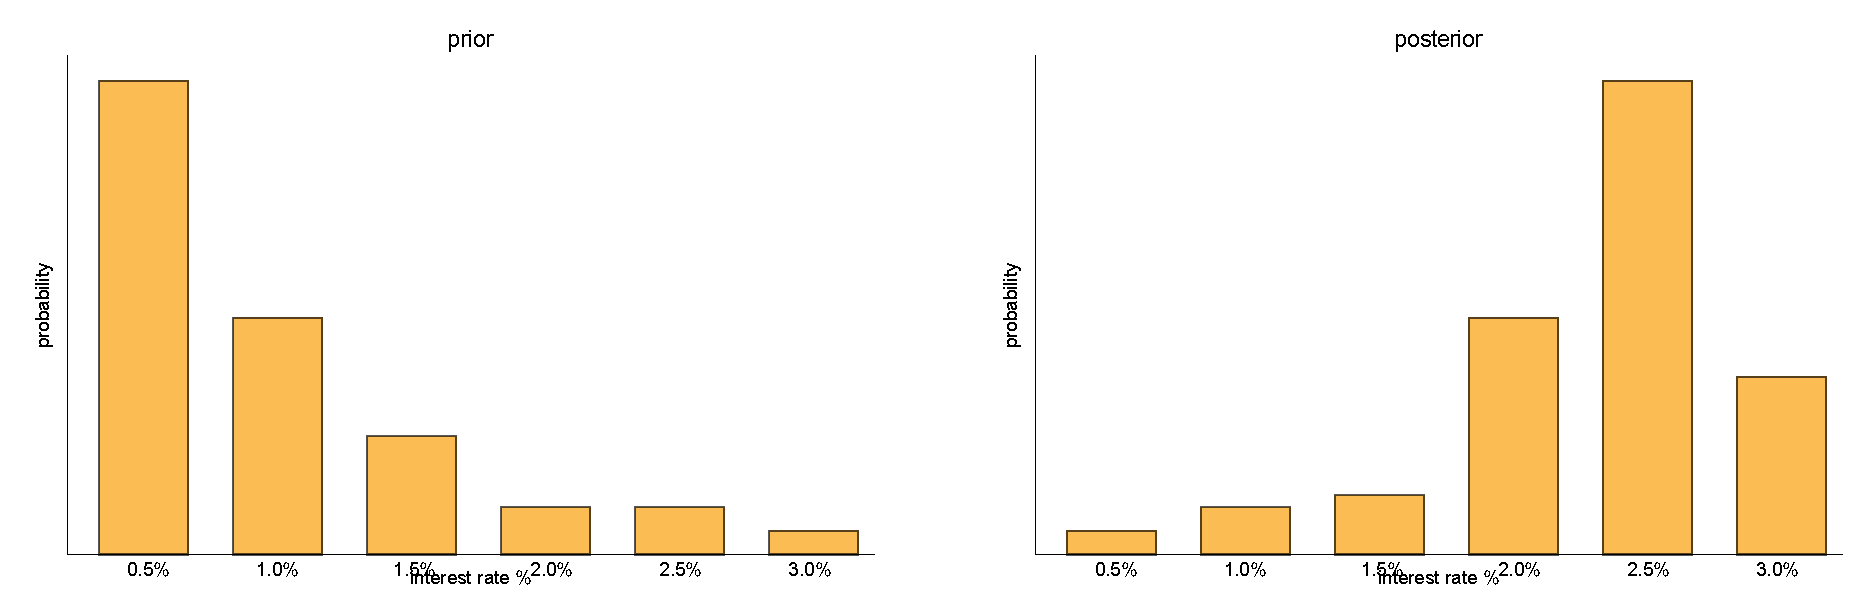
\includegraphics{Posterior_priorPosteriorInterestRate.pdf}}
\caption{The prior and posterior probabilities of different central ban interest rates.}\label{fig:Posterior_priorPosteriorInterestRate}
\end{figure}

From the prior distribution, $p(i)$, we would like to estimate the probability of particular rates of investment return. Mathematically, what we want is the marginal distribution of investment return, $p(x)$. Fortunately, we know from section \ref{sec:Probability_marginal}, that we can get a marginal distribution from a joint distribution by summing (for a discrete parameter) across values of the parameter:

\begin{align}\label{eq:Posterior_InterestpriorPredictiveDistribution}
p(x) &= \sum\limits_{i=0.5\%}^{3.0\%} p(x,i)\\
&= \sum\limits_{i=0.5\%}^{3.0\%} p(x|i) p(i)
\end{align}

This distribution essentially weights each of the conditional probabilities, $p(x|i)$, by its corresponding prior probability $p(i)$ (see the left-hand side of figure \ref{fig:Posterior_priorBuildInterestRate}), then sums them to yield the marginal probability of the data (see the right hand side of figure \ref{fig:Posterior_priorBuildInterestRate}).

\begin{figure}
\centering
\scalebox{0.4} 
{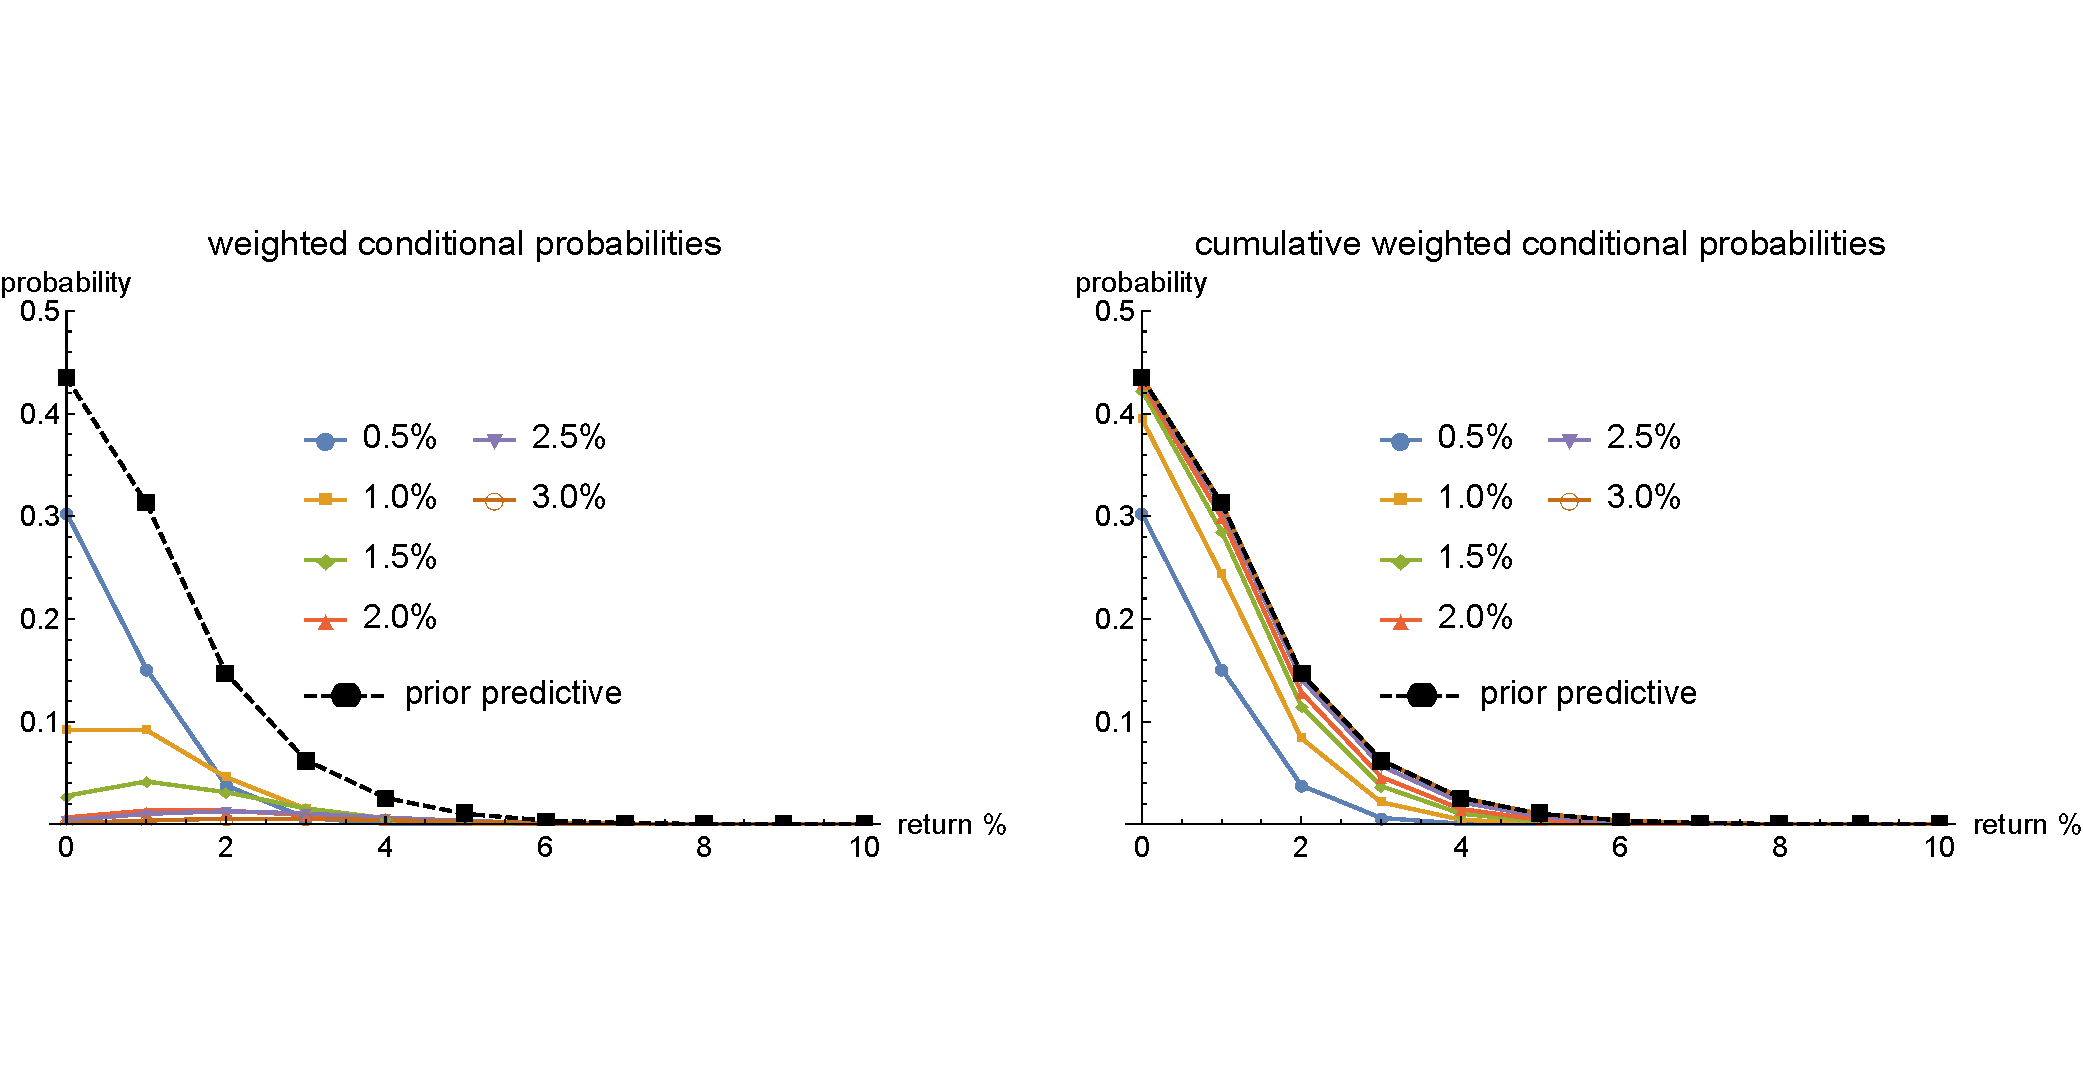
\includegraphics{Posterior_priorBuildInterestRate.pdf}}
\caption{Building the prior predictive distribution, as a sum of weighted conditional probabilities. Left: the weighted conditional probabilities (compare with figure \ref{fig:Posterior_likelihoodInterestRate}). Right: the cumulative weighted conditional probabilities, which converge on the prior predictive distribution.}\label{fig:Posterior_priorBuildInterestRate}
\end{figure}

To calculate the posterior predictive distribution, we proceed in an analogous way to the prior case. What we would like to obtain is $p(x'|x)$, where $x'$ indicates the predicted return on the investment, and $x$ represents the historical data that has been used to produce the posterior. We can again achieve this by summing out all $i$ dependence from the joint-conditional distribution $p(x',i|x)$:


\begin{align}
p(x'|x) &= \sum\limits_{i=0.5\%}^{3.0\%} p(x',i|x)\\
&= \sum\limits_{i=0.5\%}^{3.0\%} p(x'|i,x) p(i|x)\\
&= \sum\limits_{i=0.5\%}^{3.0\%} p(x'|i) p(i|x)
\end{align}

Note that we have gone from the second line to the third line, because we suppose that, once $i$ is known, the likelihood is independent of past values of $x$, and thus $p(x'|i,x)=p(x'|i)$. Also, note the similarity between this derivation and that for the prior predictive distribution in \ref{eq:Posterior_InterestpriorPredictiveDistribution}; the only difference in both second lines, is that in the posterior case, everything is conditioned on the historical values of $x$. We suppose that the likelihood function remains constant, so that like the prior predictive distribution, the posterior predictive distribution is obtained by weighting each of the conditional probability lines $p(x'|i)$ by a probability - in this case, the posterior probability for that value of $i$. 

The resultant prior and posterior distributions are shown in figure \ref{fig:Posterior_priorPosteriorPredictiveInterestRate}. We notice that the posterior predictive distribution is shifted rightwards, towards higher investment returns, because of the fact that the posterior expected interest rate is higher than for the prior case.

\begin{figure}
\centering
\scalebox{0.65} 
{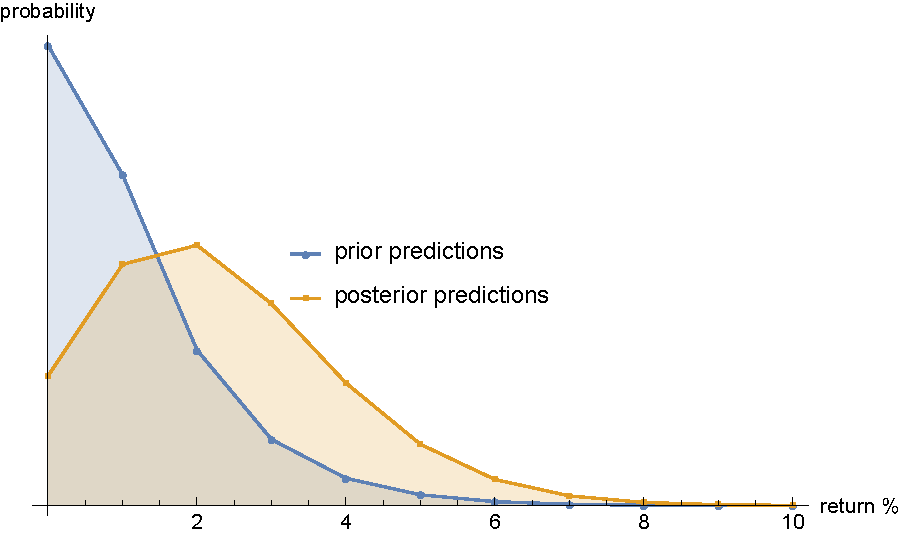
\includegraphics{Posterior_priorPosteriorPredictiveInterestRate.pdf}}
\caption{The prior and posterior predictive distributions for investment returns.}\label{fig:Posterior_priorPosteriorPredictiveInterestRate}
\end{figure}

\section{Model comparison using the posterior}
Suppose we have two competing models ($M1$ and $M2$) which we could use to explain a given dataset, and would like a way of evaluating their respective worth. The Bayesian framework can be used to incorporate the choice between two (or more) models, in a straightforward way. Suppose we denote a discrete parameter, $M\in[M1,M2]$, which indexes the choice of model. A way of gauging a model's performance is to calculate the probability of the model \textit{given} the data obtained, $p(M|data)$. Since we have introduced this new parameter $M$, we can use Bayes' rule to calculate this quantity:

\begin{equation}\label{eq:Posterior_modelGivenDataProbability}
p(M|data) = \frac{p(data|M) p(M)}{p(data)}
\end{equation}

Looking at (\ref{eq:Posterior_modelGivenDataProbability}) in detail, we examine the following quantities: $p(data|M)$, which represents what we, in the single model set-up, simply call $p(data)$; the $p(M)$ which represents our \textit{a priori} probability of each model being correct; and $p(data)$, which in this case represents the marginal probability of the model when we have summed out our dependence on the model choice:


\begin{align}
p(data) &= \sum\limits_{M=M1}^{M2} p(data,M)\\
&= \sum\limits_{M=M1}^{M2} p(data|M) p(M)\\
&= p(data|M1) p(M1) + p(data|M2) p(M2)
\end{align}

We can then calculate the ratio of the probabilities of each model, given the data obtained:

\begin{align}\label{eq:Posterior_modelComparisonFull}
\frac{p(M1|data)}{p(M2|data)} &= \frac{p(data|M1) p(M1)}{p(data|M2) p(M2)}\\
&= \frac{p(data|M1)}{p(data|M1)} \times \frac{p(M1)}{p(M2)}\\
&= BF \times \frac{p(M1)}{p(M2)}
\end{align}

If this ratio is greater than 1, then this test suggests that we should favour model 1, and vice versa if the ratio is less than 1. We have also defined a quantity, $BF$, called the \textit{Bayes Factor}:

\begin{equation}\label{eq:Posterior_bayesFactorDefinition}
BF = \frac{p(data|M1)}{p(data|M1)}
\end{equation}

This factor represents in a narrow sense, the strength of support of model 1, over model 2, provided by the data. Note that if our prior probabilities of each model are identical, $p(M1) = p(M2) = \frac{1}{2}$, then:

\begin{equation}
\frac{p(M1|data)}{p(M2|data)} = BF
\end{equation}

And the choice of model is determined solely through the Bayes Factor. 

However, there is uncertainty over when the BF is enough to prefer one model over another. Whereas a BF of 100 may be enough to prefer a given model, how about 1.01? Jeffrey's scale (introduced in chapter \ref{chap:ModelFit}), is an arbitrary, albeit industry-standard, meter to determine when a given model should be preferred over another.

Importantly we do want to state here, that this is \textit{not} the correct way to choose between competing models. We will learn a much more nuanced, and reasonable way of choosing between models when we introduce the concept of \textit{Posterior Predictive Checks} in chapter \ref{chap:ModelFit}. That is not to say that these methods introduced above can't be used as additional evidence for or against a given model, it is just that they should not be used as \textit{sole}, or even \textit{primary}, method.

\subsection{Example: epidemiologist comparison}
Suppose you find yourself in the (bizarre) situation, where you would like to compare two epidemiologists in terms of their ability to predict the underlying proportion of individuals having colds. The first epidemiologist, named \textit{optimist}, gives his estimation of the proportion of individuals with colds, $\theta$, via the (prior) distribution shown in figure \ref{fig:Posterior_bayesFactorFluEpidemiologist}. The second, named \textit{pessimist}, gives a slightly more conservative estimate of the underlying proportion of individuals with colds (also shown in figure \ref{fig:Posterior_bayesFactorFluEpidemiologist})\footnote{Here we have actually generated these priors by assuming, for the optimist, $\theta\sim Beta[3,40]$ and $\theta\sim Beta[4,15]$ for the optimist and pessimist respectively.}.

The data we have is 10 samples of 100 people, where survey respondents have indicated whether or not they are currently suffering from a cold, $\boldsymbol{x} = \{22, 18, 18, 12, 16, 15, 21, 19, 14, 15\}$. 

We can then go through and calculate the $p(data|M)$ for each of the two different priors (see figure \ref{fig:Posterior_bayesFactorFluEpidemiologist} for a graphical depiction of this), by simply integrating the joint density with respect to $\theta$:

\begin{align}
p(data) &= \int\limits_{0}^{1} p(data,\theta) \mathrm{d}\theta\\
&= \int\limits_{0}^{1} p(data|\theta) p(\theta) \mathrm{d}\theta
\end{align}

where $p(data|\theta)$ is the likelihood function\footnote{Which here is taken to be a binomial density.}. Carrying out this integrand for each of the different priors results in the probabilities of data given in the bottom panel of figure \ref{fig:Posterior_bayesFactorFluEpidemiologist}. From this, we note two things: firstly both of the probabilities are very small. This is typical, and is unsurprising when you consider the vast array of possible outcomes that could have occurred. Secondly, we see that the probability of the data for the pessimist is higher than for the optimist. Indeed, we can calculate the Bayes factor via (\ref{eq:Posterior_bayesFactorDefinition}), and find here $BF \approx 6$ for the pessimist vs the optimist model; which, if we assign equal priors to each model, results in us favouring the pessimistic perspective.

It should be added that this use of Bayes factors is atypical; it is not usually used as a means of testing between differing priors. However, since this forms part of a model, we can test its support with the data like any other part.

\begin{figure}
\centering
\scalebox{0.45} 
{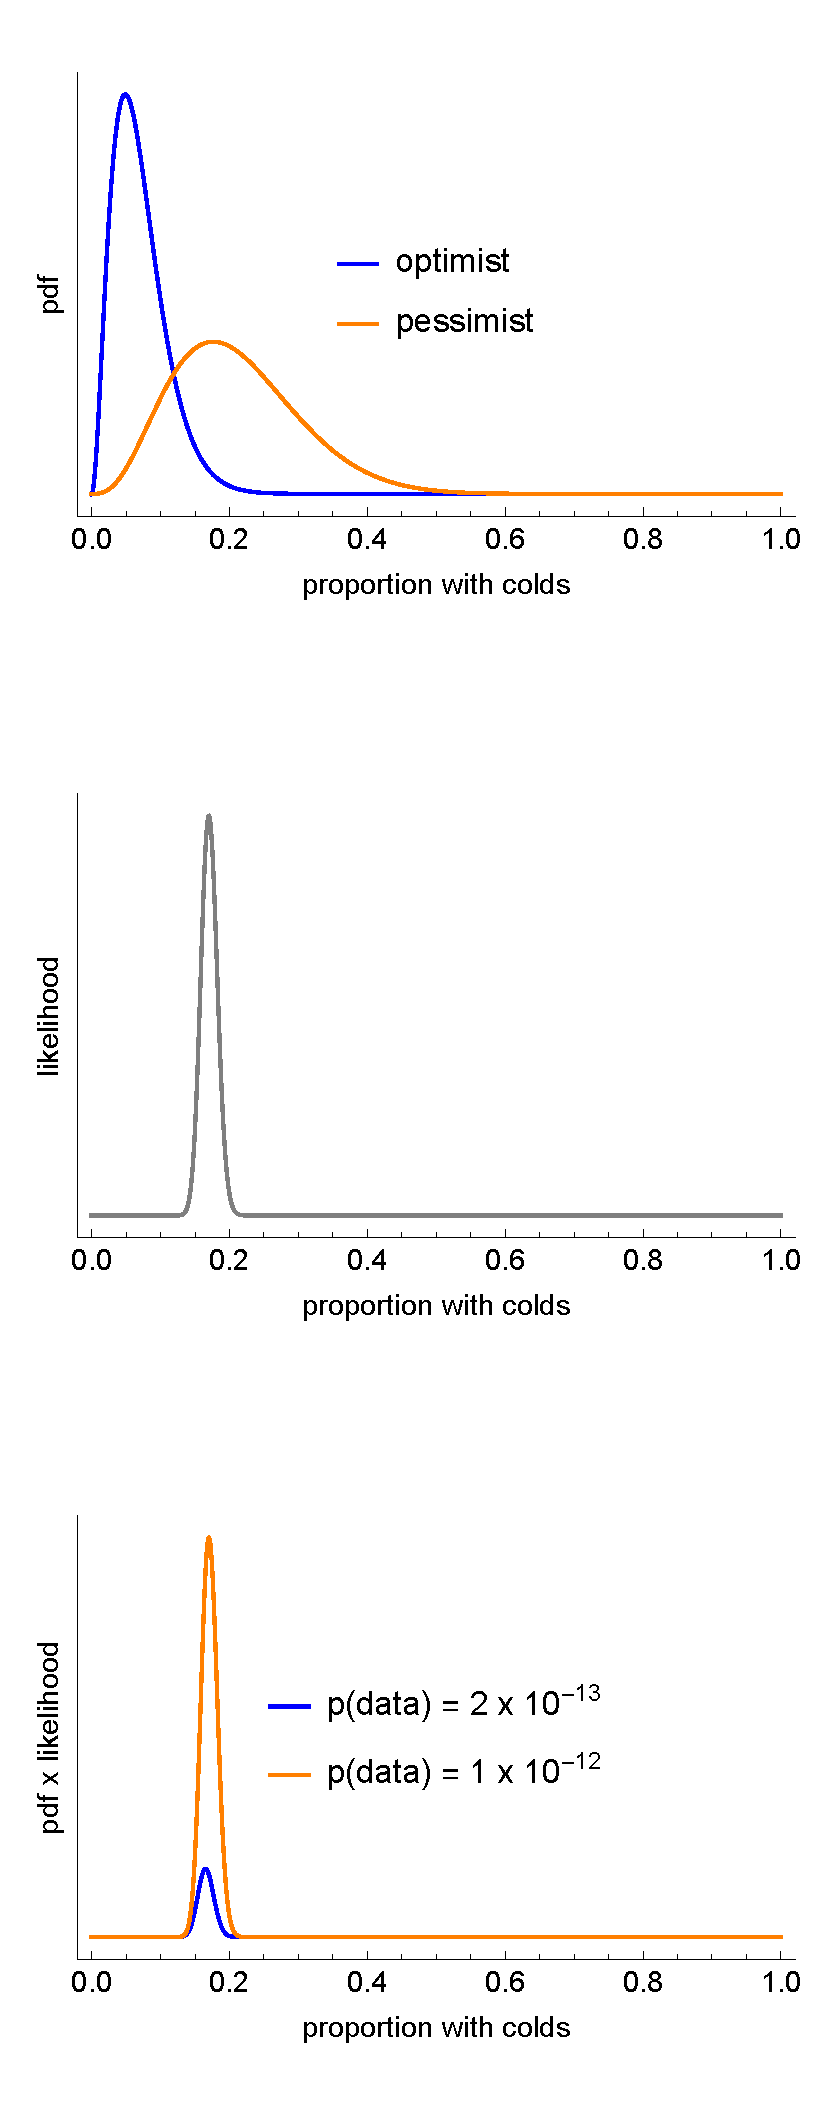
\includegraphics{Posterior_bayesFactorFluEpidemiologist.pdf}}
\caption{Calculating the probability of the data for the two epidemiologists' opinions on colds.}\label{fig:Posterior_bayesFactorFluEpidemiologist}
\end{figure}

\subsection{Example: customer footfall}
Suppose that your job at a consultancy is to try to develop a statistical model which describes the footfall of customers into a particular store location at 1pm-2pm, over a span of 2 months. We have collected the data shown in the histogram in the left hand panel of figure \ref{fig:Posterior_modelComparisonFootfall}. 

Firstly, we fit a poisson likelihood to the data, since we know that the data were collected over a fixed period of time, and we might initially posit that the entry of an individual into the store is independent of others' entry\footnote{See chapter \ref{chap:distributions} for a more complete examination of this distribution.}. However, we notice the point to the far right of the histogram. A poisson distribution is not reasonably able to cope with this degree of extremity, since it has a variance which is given by its mean - in this case this is estimated to be 10.5. For a small dataset, it seems hard to believe that a data point at 26, could have been generated from such a model\footnote{This would be more easily seen by posterior predictive checks.}.

An alternative model, which allows for a variance which exceeds its mean is the negative binomial. This choice of distribution would make most sense if we believed that one consumers' entry into a store was not independent of another's. This would make sense if people tend to shop in groups, and if the shop is outside, with people tending to enter \textit{en masse} when it rains. The expense of this extra freedom, compared to the poisson, is that it is a two-parameter distribution, opposed to a single one.

Again, we can go through and calculate the probability of the data in each case (see figure \ref{fig:Posterior_modelComparisonFootfall}), and then take the ratio to find $BF\approx 3$ for the negative binomial vs the poisson, which is unsurprising given the extreme observation. Here though, we might be tempted to \textit{a priori} favour the poisson, due to its relative parsimony; setting a prior for this model that more than accounted for its loss in explanatory power. This might mean that overall we end up using the poisson model, acknowledging its shortcomings in predicting extreme footfall. However this depends on the nature of these extreme events. If they account for a disproportionate part of sales, then it may be worth the extra flexibility of the negative binomial. If by contrast, the extreme footfall is often due to rain, where consumers simply enter to avoid getting wet, and fail to buy, we would perhaps not be so worried about the modelling of these events.

\begin{figure}
\centering
\scalebox{0.45} 
{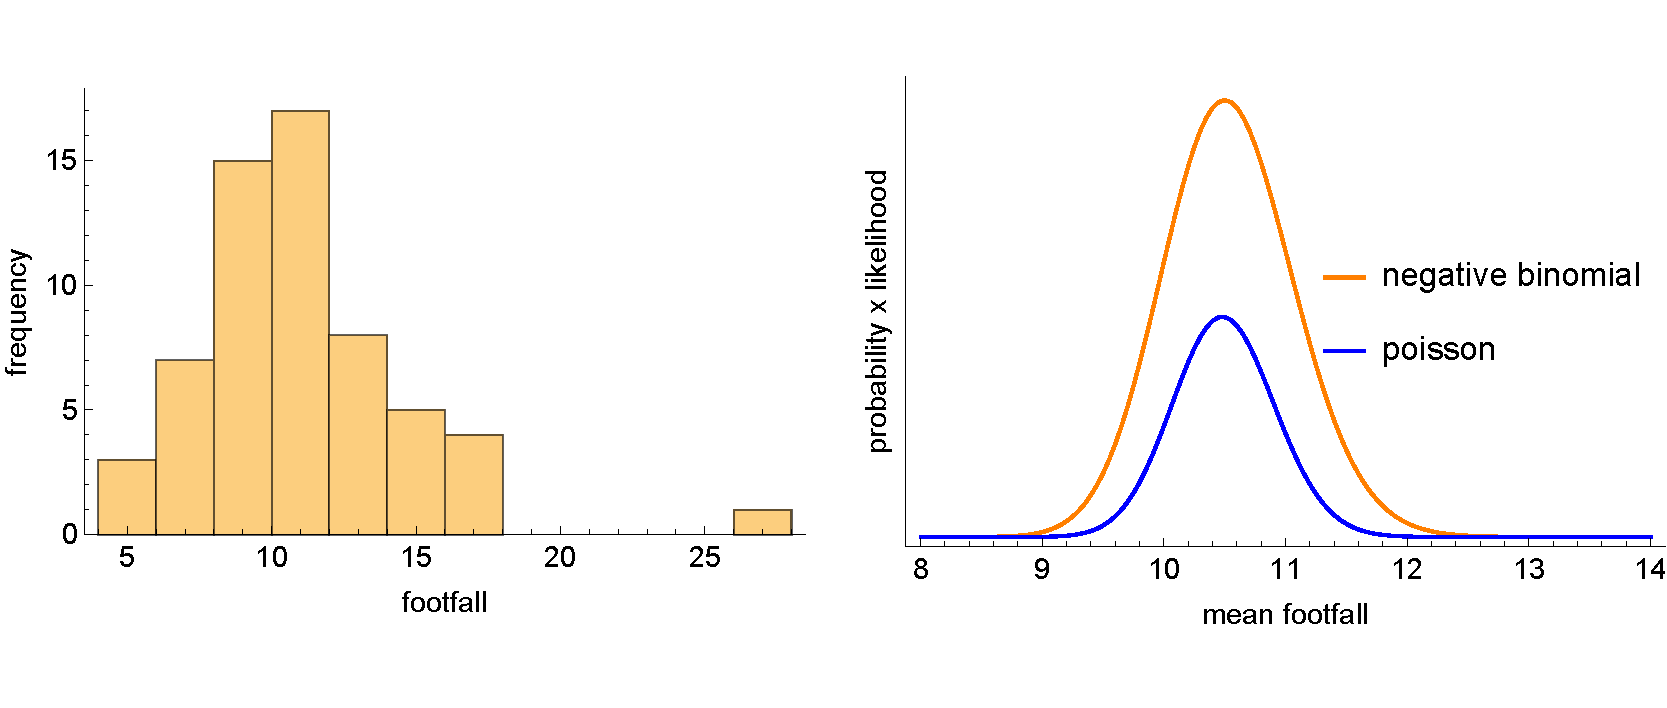
\includegraphics{Posterior_modelComparisonFootfall.pdf}}
\caption{Left: the footfall data. Right: the area under the curves represents the probability of the data from each of the two models.}\label{fig:Posterior_modelComparisonFootfall}
\end{figure}



\section{Model comparison through posterior predictive checks}
The posterior is also the predominant means for testing the worth of a model, and comparing different models. The idea behind this method is that a reasonable model should be able to \textit{simulate} data which is in some correspondence with the \textit{real} data. 

The idea behind this methodology is to simulate data, of the same dimension, and in the case of regression, with the same covariates, then compare this to the actual data. To go about simulating the data, we typically go through the following two steps:

\begin{enumerate}
\item Sample parameter values from the posterior: $\theta\sim p(\theta|x)$
\item Use these parameters in the likelihood function, then use this distribution to sample new data: $x'\sim p(x'|\theta)$
\end{enumerate}

We shall see a full description of this methodology in chapter \ref{chap:ModelFit}, so it is only mentioned here briefly as a sign of things to come. Its basic mechanism is illustrated by the following example.

\subsection{Example: stock returns}
Suppose we are tasked with modelling the daily-stock returns for a particular company over a one year period (see the leftmost panel of figure \ref{fig:Posterior_PPCstockReturns}). 

We firstly notice the symmetry of the returns, and reason that a normal likelihood may be a reasonable fit. We then use Bayes' rule, with appropriate priors (see chapter \ref{chap:conjugate} for a good guide as to appropriate priors for the parameters of a normal distribution), to calculate posteriors for the mean and variance of this distribution. We then use these posterior distributions, which are fairly narrow, to firstly sample the mean, and variance, then use a normal likelihood to simulate a number of samples of the same size as the original data. For each of the simulated series, we compare the histogram of returns to that of the actual dataset. A typical plot of this form is shown in the middle panel of figure \ref{fig:Posterior_PPCstockReturns}. We notice that the simulated data is a poor fit to the actual in a number of ways: it under-predicts the number of days with little stock movement; there are an over-abundance of days with moderate returns; and an under-weighting given to those days with more extreme stock movements. Overall, the dataset is not well represented by our model.

Instead of throwing in the towel, we decide to go for a distribution with fatter tails, which allows a greater degree of flexibility than that of a normal - a student's t distribution. We then go through the rigmarole of setting priors on its three parameters, and finally use Bayes' rule to find the posteriors of these. We then use the posterior distributions to sample these parameters, and then a t-likelihood to simulate the data a number of times. What we now typically see is a better fit (see the rightmost panel of figure \ref{fig:Posterior_PPCstockReturns}), with a similar abundance of observations near zero, and a similar distribution of extreme daily movements.

Whilst these visual checks may become cumbersome with more complex data series, it is always a good idea to at least start with them, since the eyes can often be less misleading that, for example, p-values. However, we postpone a more complete discussion of posterior predictive checks until chapter \ref{chap:ModelFit}.

\begin{figure}
\centering
\scalebox{0.35} 
{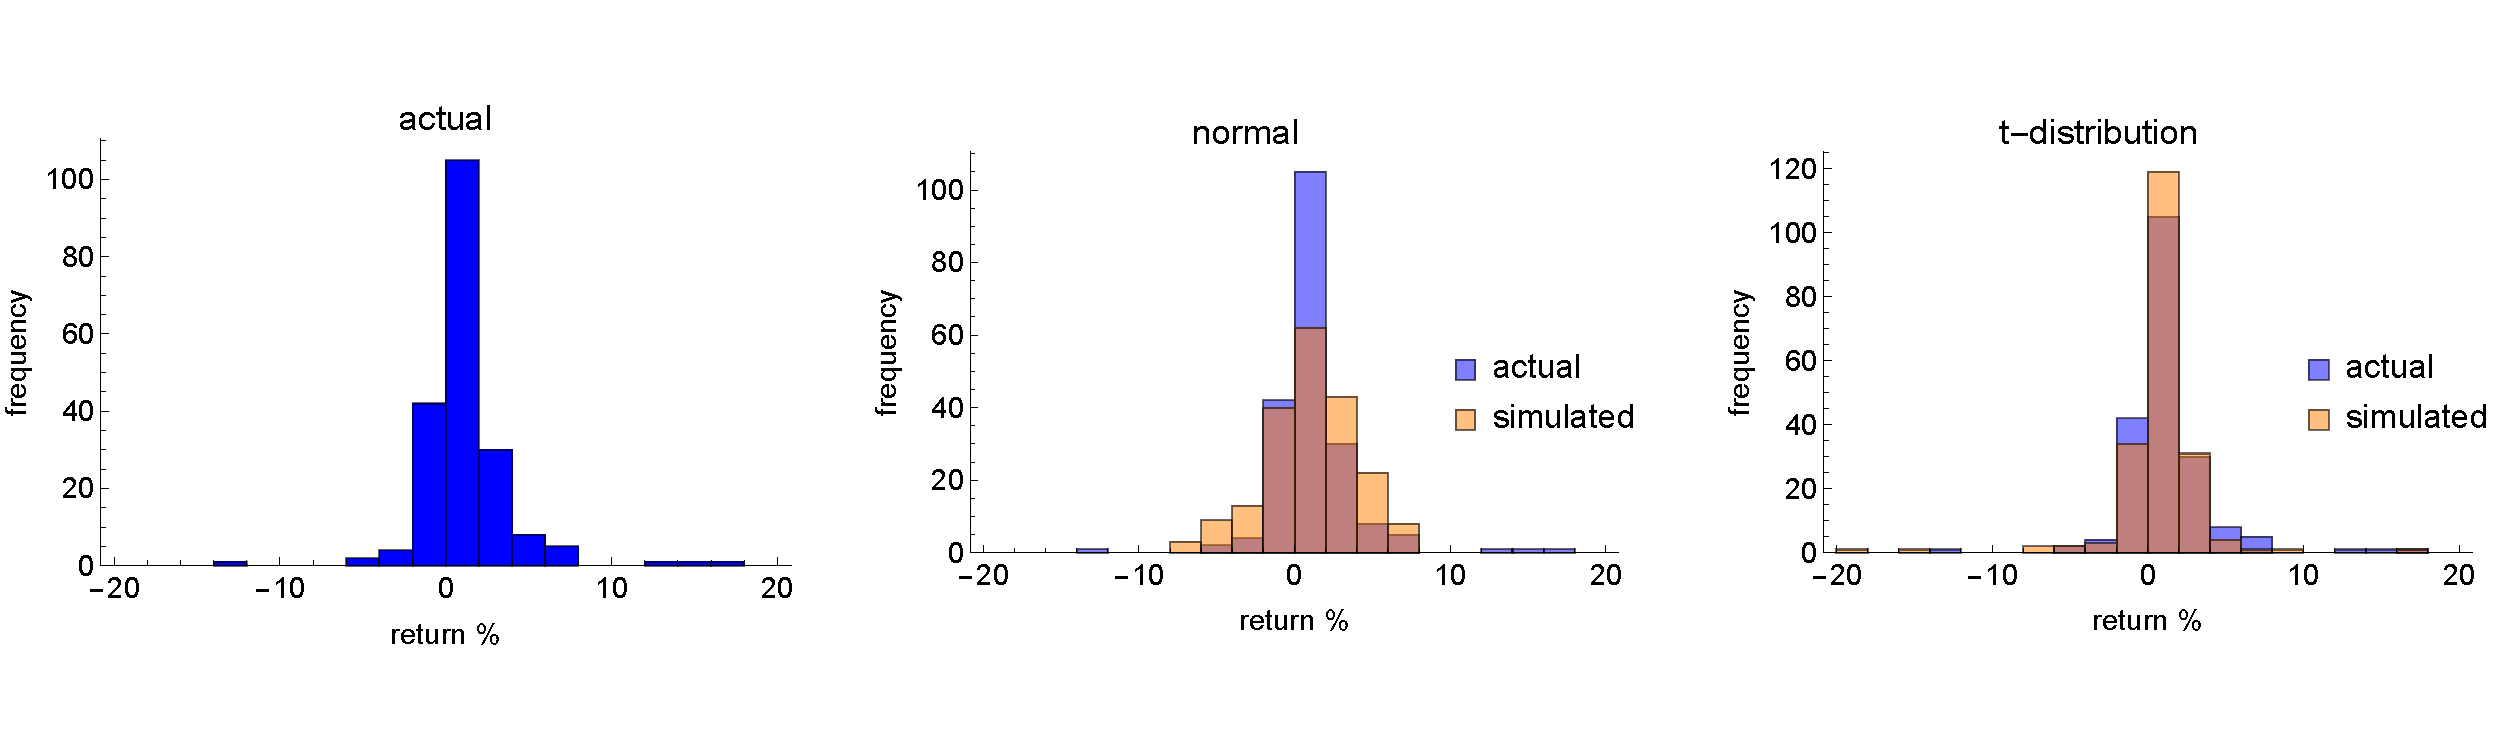
\includegraphics{Posterior_PPCstockReturns.pdf}}
\caption{Left: the actual data. Middle: actual returns vs normal-simulated returns. Right: actual returns vs t-distribution-simulated returns.}\label{fig:Posterior_PPCstockReturns}
\end{figure}


\section{Chapter summary}
In this chapter we have seen how the posterior distribution can be used to produce summaries of parameters. In particular, we have used these distributions to produce Bayesian credible intervals. We then compared and contrasted these with the classically-equivalent confidence interval, and have reasoned that in many cases the Bayesian formulation is more straightforward and intuitive than the former. We then move from the realm of the parameter, to that of the data, in order to produce prior and posterior data probabilities; which can be used to sense-check the implications of statistical models. We finally discussed methods of model comparison, introducing firstly the Bayes Factor method, followed by a short introduction to posterior predictive checks. Although the former method is common in the literature, we advocated the more nuanced approach of posterior predictive checks, albeit postponing more in-depth discussion until chapter \ref{chap:ModelFit}. Now that we have seen the utility of posterior probability distributions, we need to know how we can obtain them via Bayes' rule. In order to use the latter, we need to understand its constituent parts: the likelihood, prior and denominator. It is these three parts to which the rest of the first part of this book are devoted.

\section{Chapter outcomes}
The reader should now be familiar with the following concepts:
\begin{enumerate}
\item Expressing uncertainty in a parameter's value through probability distributions.
\item The difference between the classical confidence interval and the Bayesian credible interval.
\item Summary measures of central tendency: posterior mean and median, and MAP. The issues with the latter.
\item How to obtain the prior and posterior predictive distributions from the prior and posterior distributions respectively.
\item Model evaluation through the posterior predictive distribution.
\end{enumerate}

\section{Problem set}
\subsection{The lesser evil}
Suppose that you are a neurosurgeon and have been given the unenviable task of finding the position of a tumour within a patient's brain, and cutting it out. Along two dimensions - height and left-right axis - the tumour's position is known to a high degree of confidence. However, along the remaining axis - front-back - the position is uncertain, and cannot be ascertained without surgery. However, a team of brilliant statisticians has already done most of the job for you, and has generated samples from the posterior for the tumour's location along this axis, and is given by the data contained within the data file "data\_Posterior\_PS\_tumour.csv" .

Suppose that the more brain that is cut, the more the patient is at risk of losing cognitive functions. Additionally, suppose that the damage inflicted varies:

\begin{enumerate}
\item Linearly with the distance the surgery starts away from the tumour.
\item Quadratically with the distance the surgery starts away from the tumour.
\item There is no damage if tissue cut is within 1mm of the tumour.
\end{enumerate}

Under each of the three regimes above, find the best position along this axis from which to belong the surgery?

\subsubsection{Which of the above loss functions do you think is most appropriate, and why?}
\subsubsection{Which loss function might you choose to be most robust to \textit{any} situation?}
\subsubsection{Following from the previous point, which measure of posterior centrality might you choose?}

\subsection{Google word search prediction}
Suppose you are chosen, for your knowledge of Bayesian statistics, to work at Google as a search traffic analyst. Based on historical data you have the data shown in table \ref{tab:Posterior_PS_googleInterval} for the actual word searched, and the starting string (the first three letters typed in a search). It is your job to help make the search engines faster, by reducing the search-space for the machines to lookup each time a person types.

\begin{table}[htbp]
  \centering
    \begin{tabular}{cccc}
    \toprule
          & \textbf{Barack Obama} & \textbf{Baby clothes} & \textbf{Bayes} \\
    \midrule
    \textbf{Bar} & 50\%  & 30\%  & 30\% \\
    \textbf{Bab} & 30\%  & 60\%  & 30\% \\
    \textbf{Bay} & 20\%  & 10\%  & 40\% \\
    \bottomrule
    \end{tabular}%
  \caption{The columns give the historic breakdown of the search traffic for three topics: Barack Obama, Baby clothes, and Bayes; by the first three letters of the user's search.}\label{tab:Posterior_PS_googleInterval}%
\end{table}%


\subsubsection{Find the minimum-coverage confidence intervals of topics that exceed 70\%.}
\subsubsection{Find most narrow credible intervals for topics that exceed 70\%.}

\subsubsection{Topic search volumes}
Now we suppose that your boss gives you the historic search information shown in table \ref{tab:Posterior_PS_googleIntervalHistoricTopic}. Further, you are told that what is most important is correctly suggesting the actual topic as one of the first auto-complete options irrespective of the topic searched.

Do you prefer confidence intervals or credible intervals in this circumstance?

\begin{table}[htbp]
  \centering
    \begin{tabular}{rccc}
    \toprule
          & \textbf{Barack Obama} & \textbf{Baby clothes} & \textbf{Bayes} \\
    \midrule
    \textbf{Search volume} & 60\%  & 30\%  & 10\% \\
    \bottomrule
    \end{tabular}%
  \caption{The historic search traffic broken down by topic.}\label{tab:Posterior_PS_googleIntervalHistoricTopic}%
\end{table}%

\subsubsection{Three-letter search volumes}
Alternatively, suppose that you have the historic search volume by the starting characters of the search, shown in table \ref{tab:Posterior_PS_googleIntervalHistoricKeyword}. You are now told, that the most important thing is directing the user to the correct topic given the keyword they have started to type.

Do you prefer confidence intervals or credible intervals in this circumstance?


\begin{table}[htbp]
  \centering
    \begin{tabular}{cccc}
    \toprule
          & \textbf{Bar} & \textbf{Bab} & \textbf{Bay} \\
    \midrule
    \textbf{Search volume} & 50\%  & 40\%  & 10\% \\
    \bottomrule
    \end{tabular}%
  \caption{The historic search traffic broken down by keyword.}\label{tab:Posterior_PS_googleIntervalHistoricKeyword}%
\end{table}%


\subsection{Prior and posterior predictive example (with PPCs maybe)}
Ben to add later.

\section{Appendix}
\subsection{The interval ENIGMA - explained in full}\label{sec:Posterior_appendixConfidenceInterval}


\chapter{Likelihoods}\label{chap:Likelihoods}
\begin{quotation}
The world is everything that is the case. \textbf{Wittgenstein}
\end{quotation}

\section{Chapter Mission statement}
At the end of this chapter a reader will know how to go about selecting a likelihood which is appropriate to a given situation. Further the reader will understand the basis behind maximum likelihood estimation.

Insert a graphic with the likelihood part of Bayes' formula circled, as in the equation shown below for the part highlighted in blue.

\begin{equation}
p(\theta|data) = \frac{{\color{blue}p(data|\theta)}\times p(\theta)}{p(data)}
\end{equation}\label{eq:Likelihood_BayesHighlighted}

\section{Chapter goals}
The starting point of the right hand side of the Bayesian formula is the likelihood function. This chapter will explain what is meant by a likelihood function, and why it is incorrect to view it as a probability in Bayesian analyses. The choice over which likelihood to use for a given situation is often difficult; especially to those unfamiliar with statistics. This chapter will provide practical guidance on likelihood choice, describing a framework that can be used to select a model in a systematic way. As an important stepping stone to Bayesian estimation, this chapter will also explain how classical maximum likelihood estimation works. 

\section{What is a likelihood?}
In all statistical inference, we use an idealised, simplified, model to try to mimic relationships between real variables of interest. This model is then used to test hypotheses about the nature of the relationships between these variables. In Bayesian statistics the evidence for a particular hypothesis is summarised in posterior probability distributions. Bayes' magic rule tells us how we can compute this posterior probability distribution for a given parameter within a model, $\theta$:

\begin{equation}
p(\theta|data) = \frac{p(data|\theta)\times p(\theta)}{p(data)}
\end{equation}\label{eq:Likelihood_Bayes}

The first step to understanding this formula (so that we can ultimately use it!) is to understand what is meant by the numerator term, $p(data|\theta)$, which Bayesians call a \textit{Likelihood}. Firstly, it's important to say that what we really mean by the numerator is:

\begin{equation}
p(data|\theta) = Probability(data|\theta,Model \; Choice)
\end{equation}\label{eq:Likelihood_simple}

(\ref{eq:Likelihood_simple}) represents the probability that we would have obtained the 'data', given (this is represented by the $|$ symbol) a particular value of $\theta$ and a particular choice of model. In other words, if our statistical model were true, and the value of the model's parameter were $\theta$, (\ref{eq:Likelihood_simple}) tells us the probability that we would have obtained our data. 

But what does this mean in simple, everyday language? Imagine that we flip a \textit{fair} coin. The most simple statistical model for coin flipping we can pick is to disregard the angle it was thrown at, as well as its height above the surface, along with any other details, and just pick the probability of the coin coming heads to be $\theta=\frac{1}{2}$. Furthermore, if a coin is thrown twice, we might choose to model the situation by assuming that the throwing technique is sufficiently similar between the two throws such that we can model each throw as independently having a probability of $\frac{1}{2}$. It's important to note that it is an assumption to forget about the throwing angle, as well as height of throw for each throw, and this forms part of our model of the situation. 

We can use our simple model\footnote{Albeit in practicality, this is a pretty reasonable representation of the situation for most purposes.} to calculate the probability that we obtain two heads in a row:


\begin{align}\label{eq:Likelihood_fairCoin}
Pr(HH|\theta,Model) &= Pr(H|\theta,Model)\times Pr(H|\theta,Model)\\
&= \theta \times \theta = \theta^2\\ 
&= \frac{1}{2}\times \frac{1}{2} = \frac{1}{4}
\end{align}

The last row of (\ref{eq:Likelihood_fairCoin}) is obtained by assuming the probability of a head, $\theta=\frac{1}{2}$. If we continue to use this \textit{same} value of $\theta$, we can calculate the corresponding probabilities for all outcomes of throwing the coin twice. The most heads that can show up is 2, and the least being zero (if both flips come up tails). Figure \ref{fig:Likelihood_fairCoin} displays the probabilities for this model of the situation. The most likely number of heads to occur is 1, since this can occur in two different ways - either the first coin comes up heads, and the second is tails, or vice versa - whereas the other possibilities (all heads, or no heads) can each only occur in one way. However, the important thing to note about figure \ref{fig:Likelihood_fairCoin} isn't the individual probabilities, it is that it is a \textit{valid} probability distribution\footnote{See section \ref{sec:Probability_validProbabilityDistribution} for a refresher if you are unsure what is meant by a valid probability distribution.}, because:

\begin{itemize}
\item The individual event probabilities are all non-negative.
\item The sum of the individual probabilities is 1.
\end{itemize}

So it appears when we assume a particular value of $\theta$, and vary the data (in this case the number of heads obtained), the collection of resultant probabilities form a probability distribution. So, why do Bayesians call $p(data|\theta)$ a 'likelihood', and eschew the name 'probability'?

\begin{figure}
\centering
\scalebox{0.5} 
{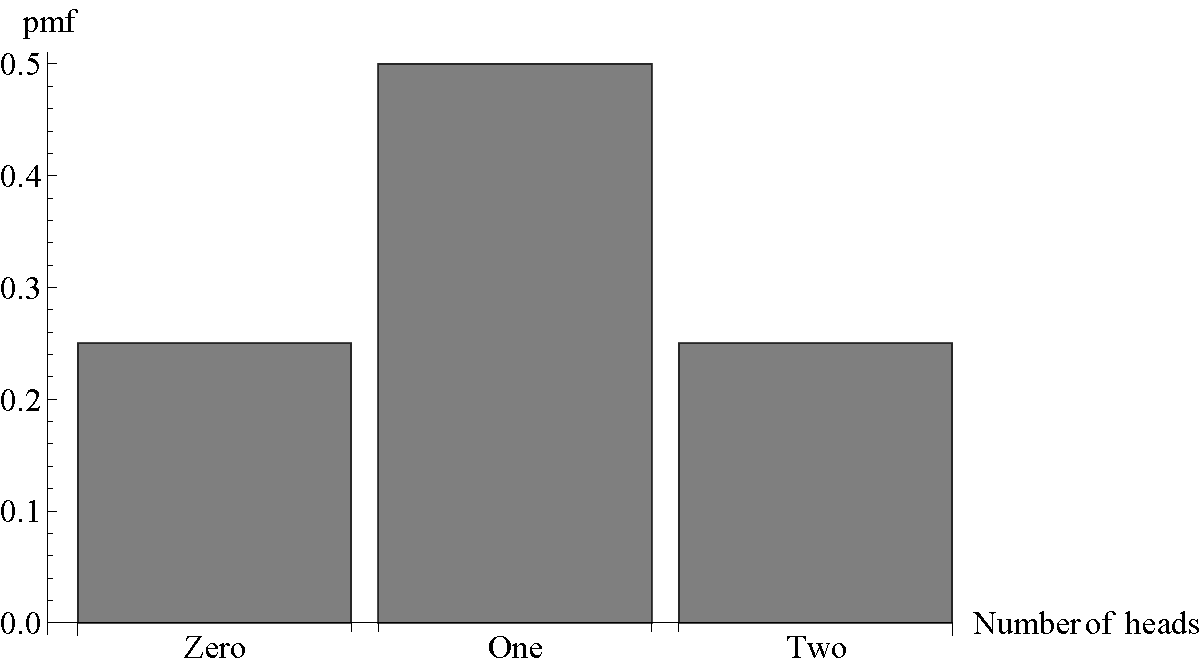
\includegraphics{Likelihood_fairCoin.pdf}}
\caption{The probabilities of all possible numbers of heads for a fair coin.}\label{fig:Likelihood_fairCoin}
\end{figure}

\section{Why use 'likelihood' rather than 'probability'?}
When we hold the parameters of our model fixed, as when we held the probability of an individual throw turning up heads, $\theta=\frac{1}{2}$, we've reasoned that the first term of the numerator of Bayes' rule in (\ref{eq:Likelihood_Bayes}) is a probability. So why don't we just keep calling it that, instead of renaming it a \textit{likelihood}? 

The reason is that in Bayesian inference, we \textit{don't} keep the parameters of our model fixed! In Bayesian analysis, it is the \textit{data} that is fixed, and the parameters that vary. This is because a posterior distribution shows the probability a parameter in a model lies in a particular range, assuming that we have obtained our particular data sample. For the case of a coin, where we don't know the probability of a head beforehand, what we hope to get out is a probability distribution of the kind shown in figure \ref{fig:Likelihood_posteriorExample}, where the x-axis is the value of $\theta$. In order to get $p(\theta|data)$ however, we must calculate $p(data|\theta)$ from the numerator of Bayes' rule in (\ref{eq:Likelihood_Bayes}) for each \textit{possible} value of $\theta$. If we assume we obtained one head and one tail, then we can calculate the probability of this occurring for a fixed $\theta$:

\begin{align}
Pr(HT|\theta) + Pr(TH|\theta) &= \theta(1-\theta) + \theta(1-\theta)
&= 2\theta(1-\theta)
\end{align}

Since we are unsure as to the 'correct' value of $\theta$, we can graph this expression as a function of this parameter, to try to understand which values of the parameter are more or less likely, given our data (see figure \ref{fig:Likelihood_coinLikelihood}).

On first glances it appears that \ref{fig:Likelihood_coinLikelihood} could be a probability distribution, but first looks can be deceiving. 

\begin{figure}
\centering
\scalebox{0.5} 
{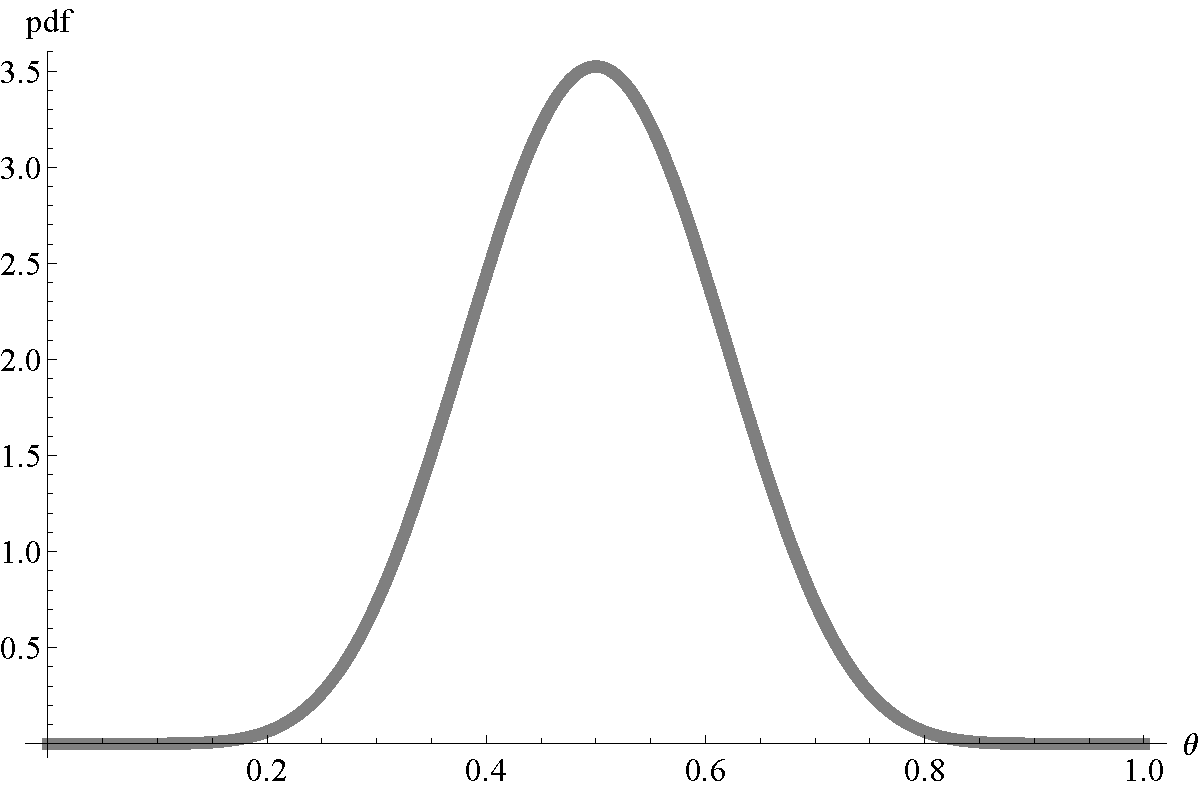
\includegraphics{Likelihood_posteriorExample.pdf}}
\caption{An example posterior distribution for the probability of obtaining a heads in a coin toss.}\label{fig:Likelihood_posteriorExample}
\end{figure}

\begin{figure}
\centering
\scalebox{0.5} 
{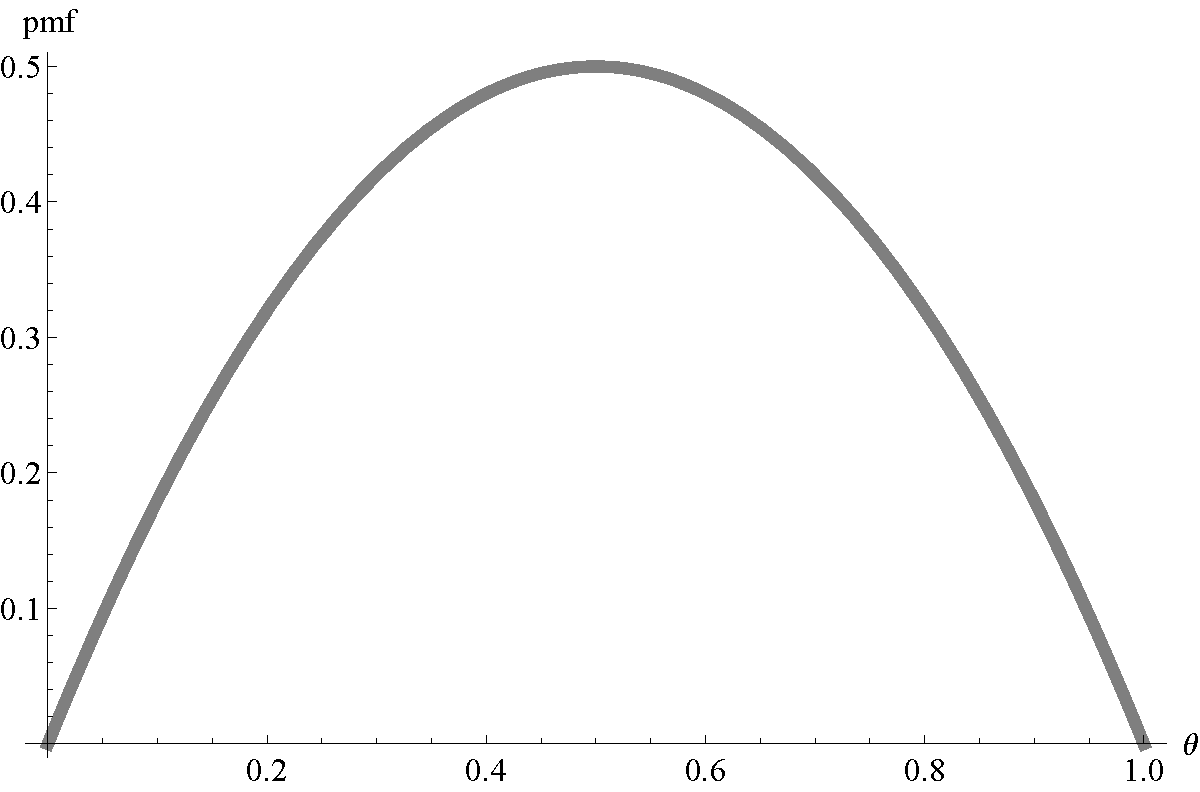
\includegraphics{Likelihood_coinLikelihood.pdf}}
\caption{The likelihood function for obtaining a single head from two throws. The area under the curve is $\frac{1}{3}$.}\label{fig:Likelihood_coinLikelihood}
\end{figure}

Checking off our necessary components of a probability distribution, we first note that all the values of the distribution in figure \ref{fig:Likelihood_coinLikelihood} are non-negative; which is what we require. However, if we calculate the area underneath the curve in figure \ref{fig:Likelihood_coinLikelihood}:

\begin{equation}
\mathrm{I} = \int\limits_{0}^{1} 2\theta(1-\theta)\mathrm{d}\theta = \frac{1}{3} \neq 1
\end{equation}

we find that it does not integrate to 1. Thus we have a violation of the second condition for a valid probability distribution. Hence, when we vary $\theta$ we find that, $p(data|\theta)$ is not a valid probability distribution! We thus introduce the term 'likelihood' to represent $p(data|\theta)$ when we vary the parameter, $\theta$. Often the following notation is used to emphasise that likelihood is a function of the parameter $\theta$ with the data held fixed:

\begin{equation}\label{eq:Likelihood_notation}
\mathcal{L}(\theta|data) = p(data|\theta)
\end{equation}

However, in this book, we will persist with the original notation as this is most typical in the literature, under the implicit assumption that when we vary the parameters in question, the term is not strictly a probability.

To provide further justification for this argument, consider the following (albeit contrived) example. Suppose that, we throw a coin twice, and we are told beforehand that the probability of obtaining a head on a particular throw is one of six discrete values: $\theta\in\{0.0,0.2,0.4,0.6,0.8,1.0\}$. We can then use our model to calculate the probability of obtaining a number of heads, $X$:

\begin{align}\label{eq:Likelihood_OneHead}
Pr(X = 0|\theta)& = Pr(TT|\theta) = Pr(T|\theta)\times Pr(T|\theta) = (1-\theta)^2\\
Pr(X = 1|\theta)& = Pr(HT|\theta) + Pr(TH|\theta) = 2\times Pr(T|\theta)\times Pr(H|\theta) = 2\theta(1-\theta)\\\label{eq:Likelihood_TwoHead}
Pr(X = 2|\theta)& = Pr(HH|\theta) = Pr(H|\theta)\times Pr(H|\theta) = \theta^2
\end{align}

In (\ref{eq:Likelihood_OneHead}), the probability is simply given by the product of the probabilities of not obtaining a head on the first throw, $(1-\theta)$, by the probability of not obtaining a head in the second\footnote{Since we have assumed a model whereby the results of the first and second throws are independent, conditional on $\theta$. In other words, all the similarity between the two throws is captured in the parameter $\theta$.}, which is also $(1-\theta)$. The factor of two arises in (\ref{eq:Likelihood_TwoHead}) since there are two ways of getting one head: \{HT,TH\}.

We can represent the corresponding values of likelihood/probability as is shown in table \ref{tab:Likeihood_BayesBox}. In this form we can see the impact of varying the data (moving along each row), and contrast it with the effect of varying $\theta$ (moving down each column). Note that if we hold the parameter fixed - regardless of this initial choice of $\theta$ - and move along each row summing the entries, we find that the values sum to 1; meaning that this is a valid probability distribution. By contrast, when we hold the number of heads fixed, and vary the parameter $\theta$, moving down each column, summing the entries, we find that the values do not sum to 1. Hence, when we vary $\theta$, we are not dealing with a proper probability distribution, meriting the use of the term 'likelihood'.

In Bayesian inference, we always vary the parameter, and implicitly hold the data fixed. Thus, from a Bayesian perspective it is important to use the term \textit{likelihood} to indicate that we recognise we are not dealing with a probability distribution.


\begin{table}[htbp]
  \centering
  
    \begin{tabular}{ccccc}
    \multicolumn{5}{c}{\textbf{Number of heads}} \\
    \midrule
    \textbf{$\theta$} & \multicolumn{1}{c}{\textbf{0}} & \multicolumn{1}{c}{\textbf{1}} & \multicolumn{1}{c}{\textbf{2}} &  \multicolumn{1}{c}{\textbf{Total}} \\
    \hline
    \textbf{0.0} & \multicolumn{1}{c}{1.00} & \multicolumn{1}{c}{0.00} & \multicolumn{1}{c}{0.00} & \multicolumn{1}{c}{\textbf{1.00}} \\
    \textbf{0.2} & \multicolumn{1}{c}{0.64} & \multicolumn{1}{c}{0.32} & \multicolumn{1}{c}{0.04} & \multicolumn{1}{c}{\textbf{1.00}} \\
    \textbf{0.4} & \multicolumn{1}{c}{0.36} & \multicolumn{1}{c}{0.48} & \multicolumn{1}{c}{0.16} & \multicolumn{1}{c}{\textbf{1.00}} \\
    \textbf{0.6} & \multicolumn{1}{c}{0.16} & \multicolumn{1}{c}{0.48} & \multicolumn{1}{c}{0.36} & \multicolumn{1}{c}{\textbf{1.00}} \\
    \textbf{0.8} & \multicolumn{1}{c}{0.04} & \multicolumn{1}{c}{0.32} & \multicolumn{1}{c}{0.64} & \multicolumn{1}{c}{\textbf{1.00}} \\
    \textbf{1.0} & \multicolumn{1}{c}{0.00} & \multicolumn{1}{c}{0.00} & \multicolumn{1}{c}{1.00} & \multicolumn{1}{c}{\textbf{1.00}} \\
    \bottomrule
    \textbf{Total} & \multicolumn{1}{c}{\textbf{1.20}} & \multicolumn{1}{c}{\textbf{1.60}} & \multicolumn{1}{c}{\textbf{2.20}} &  \\
    
    \end{tabular}%
  %
  \caption{The values of likelihood for the case of tossing a coin twice, where the probability of heads is constrained to take on a discrete value: \{0.0,0.2,0.4,0.6,0.8,1.0\}.}\label{tab:Likeihood_BayesBox}
\end{table}

\section{What are models and why do we need them?}
All models are wrong. They are idealised representations of reality resultant from making assumptions, which if reasonable, may emulate some of the behaviour of a system of interest. Joshua Epstein in an article titled, 'Why model?' emphasises that we perennially build \textit{implicit} mental models for various phenomena \cite{epstein2008model}. Before we go to bed at night we set our alarms for the next morning on the basis of a model. We imagine an idealised - model - morning when it takes us 15 minutes to wake up as a result of an alarm. We use this model to predict how long it will take us to rise from bed, shower, and get changed into clothes in sufficient time to get to work. Whenever we go to the Doctor, they use an internalised biological model of the human body to advise on the best course of treatment for a particular ailment. Whenever we hear expert opinions on TV about the outcome of an upcoming election, the pundits are using mental models of society to explain the results of current polls, as well as make forecasts. As is the case with all models, some are better than others. Hopefully, the models a Doctor uses to prescribe medicine are subject to less error than the opinions of pundits seen on TV\footnote{For a great discussion of the performance of TV pundits, read Thinking Fast. Insert reference}! 

Epstein goes on to emphasise that the question, 'Why model?' really means why should we build an \textit{explicit} - written down - model of phenomena? The point being that \textit{implicit} models are by their very nature, opaque, and not subject to the sort of interrogation that can be obtained by writing the model on paper. 

We can also ask more narrowly, what are we hoping to gain by building an \textit{explicit} model of a situation? Epstein suggests the following motivations:

\begin{itemize}
\item Prediction
\item Explanation
\item Guide data collection
\item Discover new questions
\item Bound outcomes to plausible ranges
\item Illuminate uncertainties
\item Challenge the robustness of prevailing theory through perturbations
\item Reveal the apparently simple (complex) to be complex (simple) 
\end{itemize}

There are of course other reasons to build models, but we believe that this list is a reasonable starting point. However, we should not think of this list as static. Whenever we build a model, whether it is statistical, biological or sociological, we should ask, 'What are we hoping to gain by building this model, and how can I judge its success?'. Only when we have a grasp on the answers to these basic questions should we proceed to model building.

\section{How to choose an appropriate likelihood?}\label{sec:chooseLikelihood}
Bayesians are acutely aware that their models are wrong. At best the abstraction from reality allows us to explain some aspect of real behaviour; at worst they can be very misleading. Before we use a model for prediction, we require that it can explain some reasonable proportion of the system's behaviour for the past and present. With this in mind we introduce the following model selection framework:

\begin{enumerate}
\item Write down the real life behaviour/data patterns that the model should be capable of explaining.
\item Write down the assumptions that it is believed are reasonable in order to achieve the above point.
\item Search the literature for models which utilise these assumptions; extracting only the relevant components.
\item Test your model's ability to explain said behaviour/data patterns. If unsuccessful go back to the second step and re-evaluate the appropriateness of your assumptions.
\end{enumerate}

Whilst this methodology is useful for building a statistical model in general, it is more applicable for use with a full Bayesian model, resulting in a posterior distribution. In which case how do we go about specifying a likelihood for a given situation? To answer this we will start with going through a few simple examples. For a quick graphical guide to choosing an appropriate likelihood, we refer the reader to figure \ref{fig:Distributions_likelihoodTree}.

\subsection{A likelihood model for an individual's disease status}\label{sec:Likelihood_individualDisease}
Suppose we work for the State as a healthcare analyst, and we want to build a statistical model to explain the prevalence of a certain disease within a sample, which can then be used to make inferences about the population incidence. Also, (unrealistically) let's imagine that we start off with a sample of only one person, for whom we have no prior information. Let the disease status of that individual be denoted by the variable $X$ which takes on the following binary outcome values dependent on the disease status the individual:

\begin{equation}
X =
\begin{cases}
O & , No\; disease \\
1 & , Positive \; diagnosis
\end{cases}
\end{equation}

The goal of our model is to output a probability that this individual has the disease. We might assume that a fraction $\theta$ of the population has the disease, and that this individual has come from that population. For each possible outcome, we can use this simple model to calculate the probability of each outcome:

\begin{align}\label{eq:Likelihood_SimpleModel1}
Pr(X = 0|\theta)& = (1-\theta)\\
Pr(X = 1|\theta)& = \theta\label{eq:Likelihood_SimpleModel2}
\end{align}

Note the similarity between these probabilities and those of the coin flipping example in the previous section. Often, a given model can be reused in a multitude of different settings.

However, we would like to write down a single rule which yields (\ref{eq:Likelihood_SimpleModel1}) or (\ref{eq:Likelihood_SimpleModel2}) respectively, dependent on whether $X=0$ or $X=1$. This can be achieved with the following:

\begin{equation}\label{eq:Likelihood_bernoulli}
Pr(X=\alpha|\theta) = \theta^\alpha(1-\theta)^{1-\alpha}
\end{equation}

Note that in (\ref{eq:Likelihood_bernoulli}) that $\alpha\in\{0,1\}$ refers to the numeric value taken by the variable $X$. The function (\ref{eq:Likelihood_bernoulli}) is known as a \textit{Bernoulli} probability density.

Although this rule for calculating a probability of a particular disease status, $\alpha$, looks complex, we see that it reduces to (\ref{eq:Likelihood_SimpleModel1}) and (\ref{eq:Likelihood_SimpleModel2}) if the individual is disease -negative/-positive respectively:

\begin{align}\label{eq:Likelihood_SimpleModel3}
Pr(X = 0|\theta)& = \theta^0(1-\theta)^1 = (1-\theta)\\
Pr(X = 1|\theta)& = \theta^1(1-\theta)^0 = \theta\label{eq:Likelihood_SimpleModel4}
\end{align}

When we hold the datum $X$ fixed and vary $\theta$, (\ref{eq:Likelihood_bernoulli}) represents a likelihood. However, figure \ref{fig:Likelihood_bernoulli} shows that for a fixed value of $theta$ the sum (here we mean the vertical sum) of the two probability densities is always equal to 1; demonstrating that in this case (\ref{eq:Likelihood_bernoulli}) is a valid probability density. Notice also in figure \ref{fig:Likelihood_bernoulli} that the sum of probability density is defined continuously on $\{0,1\}$, whereas the sum of likelihoods is discrete.

\begin{figure}
\centering
\scalebox{0.75} 
{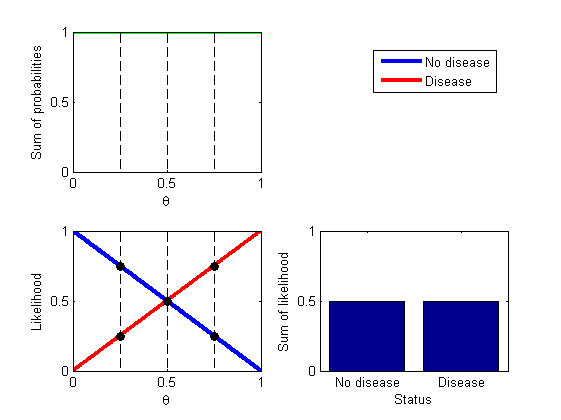
\includegraphics{likelihood_bernoulli.png}}
\caption{The likelihood function as theta varies for the case of the two possible data. The sum of likelihoods is found by the area under each line, whereas the sum of probabilities is a discrete sum.}\label{fig:Likelihood_bernoulli}
\end{figure}

\subsection{A likelihood model for disease prevalence of a group}\label{sec:Likelihood_diseaseGroup}
Now we imagine that instead of this solitary individual, we have a group of $N$ individuals. What we would like to do is to develop a model which will tell us the probability of obtaining $Z$ disease cases within our sample. We would also like to be able to use our model to predict the most likely number of individuals who have the disease in a sample, for a given value of the parameters\footnote{We are starting off by assuming that we know the parameters. Later in this chapter we will obtain a point estimate of the parameters using \textit{Maximum likelihood} estimation.}. 

In order to write down a model we first need to make some simplifying assumptions. We might assume that one individual's disease status tells us nothing about the probability of another individual in the sample having the disease\footnote{Other than, if the disease prevalence were unknown, through our ability to estimate overall disease prevalence from their individual statuses.}. This would not be a reasonable assumption if the disease were contagious, and if the individuals in the sample came from the same neighbourhood or household. It also would not be a good assumption if (as is often the case with volunteer-dependent studies) the individuals who volunteered for the experiment, self-selected on the basis of some common pre-existing ailment/underlying-factor. If an advert for participants reads, 'Psychological experiment on sleep disorders: participants wanted', we might suspect that there would be an over-presence of insomniacs than is found in the population as a whole. This first assumption is that which in statistical language we call 'independence'. We also suppose that all individuals in our sample come from the same population - the one we are trying to draw conclusions about. If we knew beforehand that some individuals came from different populations, with significantly different prevalence rates, then we might abandon this assumption. Combining these two assumptions we say in statistical language that our data sample is \textit{independent} and \textit{identically-distributed}.

With our two assumptions in hand, we can begin to formulate a model for the probability of obtaining $Z$ disease-positive individuals out of a total of $N$ individuals. We start by considering each person's disease status individually, meaning we can reuse (\ref{eq:Likelihood_bernoulli}):

\begin{equation}\label{eq:Likelihood_bernoulli1}
Pr(X=\alpha|\theta) = \theta^\alpha(1-\theta)^{1-\alpha}
\end{equation}

Note that in (\ref{eq:Likelihood_bernoulli1}) the $\alpha\in\{0,1\}$ refers to a particular numeric value taken by the variable $X$. The assumption of \textit{independence} means that we can get the overall probability by multiplying together the individual probabilities\footnote{See section \ref{sec:Probability_independence} for an explanation of this.}. In words, we obtain the probability that the first person has disease status $X_1$ \textit{and} the second person has status $X_2$:

\begin{align}\label{eq:Likelihood_bernoulli2}
Pr(X_1=\alpha_1,X_2=\alpha_2|\theta_1,\theta_2) &= Pr(X_1=\alpha_1|\theta_1)\;\times \;Pr(X_2=\alpha_2|\theta_2)\\
 &= \theta_1^{\alpha_1}(1-\theta_1)^{1-\alpha_1}\times \theta_2^{\alpha_2}(1-\theta_2)^{1-\alpha_2}
\end{align}

In (\ref{eq:Likelihood_bernoulli2}) we have assumed that each individual has a different predisposition to having the disease, denoted by $\theta_1$ and $\theta_2$ respectively.

The second assumption of \textit{identically-distributed} individuals means that we can set $\theta_1=\theta_2$:

\begin{align}\label{eq:Likelihood_bernoulli3}
 Pr(X_1=\alpha_1,X_2=\alpha_2|\theta) &= \theta^{\alpha_1}(1-\theta)^{1-\alpha_1}\times \theta^{\alpha_2}(1-\theta)^{1-\alpha_2}\\
&= \theta^{\alpha_1+\alpha_2}(1-\theta)^{2-\alpha_1-\alpha_2}
\end{align}

In (\ref{eq:Likelihood_bernoulli3}) we have obtained the second line by using the simple exponent rule: $a^b\times a^c = a^{b+c}$, for the components $\theta$ and $(1-\theta)$ respectively.

For our sample of 2 we are now in a position to calculate the probability that we obtain $Z$ cases of the disease. We first realise that we can get from $X_1$ and $X_2$ to $Z$ by:

\begin{equation}\label{eq:Likelihood_binomialTwo}
Z = X_1 + X_2
\end{equation}

We can then use (\ref{eq:Likelihood_bernoulli3}) to generate the respective probabilities.

\begin{align}\label{eq:Likelihood_binomialTwoProbs}
Pr(Z = 0|\theta)& = Pr(X_1=0,X_2=0|\theta) = \theta^{0+0}(1-\theta)^{2-0-0} = (1-\theta)^2\\
Pr(Z = 1|\theta)& = Pr(X_1=1,X_2=0|\theta) + Pr(X_1=0,X_2=1|\theta)= 2\theta(1-\theta)\\
Pr(Z = 2|\theta)& = Pr(X_1=1,X_2=1|\theta) = \theta^{1+1}(1-\theta)^{2-1-1} = \theta^2
\end{align}

To complete our probability model we want to write out a single rule for calculating the probability of any value taken on by $Z$. To do this we note that we could rewrite (\ref{eq:Likelihood_binomialTwoProbs}) as:

\begin{align}\label{eq:Likelihood_binomialTwoProbsSimple}
Pr(Z = 0|\theta)& = \;\theta^0(1-\theta)^2\\
Pr(Z = 1|\theta)& = 2\theta^1(1-\theta)^1\\
Pr(Z = 2|\theta)& = \;\theta^2(1-\theta)^0
\end{align}

In (\ref{eq:Likelihood_binomialTwoProbsSimple}) we notice the common term $\theta^\beta (1-\theta)^{2-\beta}$ in each of the expressions, where $\beta\in\{0,1,2\}$ represents the number of disease cases found. Therefore this suggests that we may be able to write down a single rule as something similar to:

\begin{equation}\label{eq:Likelihood_binomialNearly}
Pr(Z = \beta|\theta) \sim \theta^\beta(1-\theta)^{2-\beta}
\end{equation}

The only problem with matching (\ref{eq:Likelihood_binomialNearly}) with the previously obtained result is the factor of 2 on the middle line of (\ref{eq:Likelihood_binomialTwoProbsSimple}). However, as a complete aside we note that when we expand a quadratic factor we get the following:

\begin{equation}\label{eq:Likelihood_quadratic}
(x+1)^2 = x^2 + 2x + 1
\end{equation}

The numbers $\{1,2,1\}$ correspond here to the non-b-dependent coefficients of $\{x^2,x^1,x^0\}$ respectively. This sequence of numbers normally appears in early secondary school maths classes, and is either known as the binomial expansion coefficients or simply $^nC_r$. The expansion coefficients are normally written in compact form:

\begin{equation}\label{eq:Likelihood_nCr}
{2 \choose \beta} = \frac{2!}{(2-\beta)!\beta!}
\end{equation}

In (\ref{eq:Likelihood_nCr}) the $!$ has its usual meaning of factorial, and $\beta\in\{0,1,2\}$. We can therefore use this notation to help us to write down a single model for the probability of obtaining $Z$ disease cases out of a total of 2 individuals using our model:

\begin{equation}\label{eq:Likelihood_binomialTwoFull}
Pr(Z=\beta|\theta) = {2 \choose \beta} \theta^\beta (1-\theta)^{2-\beta}
\end{equation}

This likelihood function is illustrated for the three possible numbers of disease cases in figure \ref{fig:Likelihood_binomial}.

\begin{figure}
\centering
\scalebox{0.75} 
{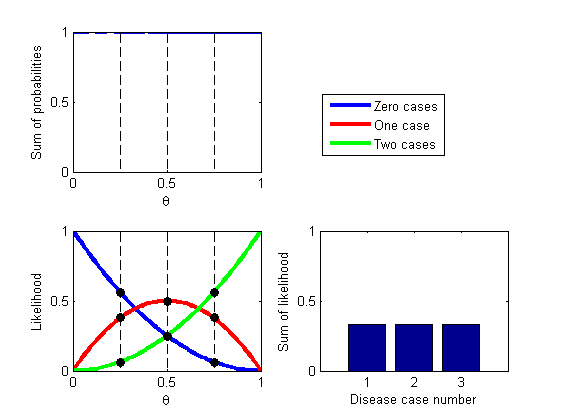
\includegraphics{likelihood_binomial.png}}
\caption{The likelihood function as theta varies for a sample of 2 individuals.}\label{fig:Likelihood_binomial}
\end{figure}

We will now extend the analysis to cover the case when we have groups of $N$ individuals. Firstly, consider the case when we have a group size of 3. If we assume that the individuals are identically distributed, then the 4 probabilities are of the form:

\begin{align}\label{eq:Likelihood_binomialThreeProbsSimpler}
Pr(Z = 0|\theta)& = \;Pr(X_1=0|\theta) Pr(X_2=0|\theta)  Pr(X_3=0|\theta)\\
Pr(Z = 1|\theta)& = 3Pr(X_1=1|\theta) Pr(X_2=0|\theta)  Pr(X_3=0|\theta)\\
Pr(Z = 2|\theta)& = 3Pr(X_1=1|\theta) Pr(X_2=1|\theta)  Pr(X_3=0|\theta)\\
Pr(Z = 3|\theta)& = \;Pr(X_1=1|\theta)Pr(X_2=1|\theta) Pr(X_3=1|\theta)
\end{align}

Again, we notice a numeric pattern in terms of the first part of each expression $\{1,3,3,1\}$, which happens to correspond exactly to the coefficients on terms for the expansion of $(x+1)^3$. Hence, we can again rewrite the likelihood using the binomial expansion notation:

\begin{equation}\label{eq:Likelihood_binomialThreeFull}
Pr(Z=\beta|\theta) = {3 \choose \beta} \theta^\beta (1-\theta)^{3-\beta}
\end{equation}

We recognise a pattern in the likelihoods of (\ref{eq:Likelihood_binomialTwoFull}) and (\ref{eq:Likelihood_binomialThreeFull}) which allows us to deduce that, for a sample size of N, the likelihood is given by:

\begin{equation}\label{eq:Likelihood_binomialNFull}
Pr(Z=\beta|\theta) = {N \choose \beta} \theta^\beta (1-\theta)^{N-\beta}
\end{equation}

(\ref{eq:Likelihood_binomialNFull}) is known as the \textit{binomial} probability distribution.

If we had data, then we could test whether the assumptions made were appropriate by calculating the model-implied-probability of this outcome. For example, if we had a sample of 100 people of which 10 were disease-positive, and we assumed beforehand that the proportion of the population who have the disease is $\theta=1\%$, then we could calculate the probability that we would have achieved a number of cases as bad, or worse than this using (\ref{eq:Likelihood_binomialNFull}):

\begin{equation}
Pr(Z\geq 10|\theta=0.01) = \sum\limits_{Z=10}^{100}{100 \choose Z} 0.01^Z (1-0.01)^{100-Z} = 7.63 \times 10^{-8}
\end{equation}\label{eq:Likelihood_binomialTest}

We have summed over all the disease cases from 10 to 100 here, because we wanted the probability that we would have obtained a result as bad, or worse, than the one which we actually achieved. This is a particular way of carrying out classical hypothesis tests, which we will dispense with later on, but for now it seems a reasonable way of testing our model. 

The probability found in this case is extremely small. What does this tell us? Well, it basically says that there is something wrong with our model which we have chosen here. It could be that the actual disease incidence in the population is much higher than the 1\% which we have assumed beforehand. It could also be that our assumption of  \textit{independence} is violated in this case, for example if we sampled whole households rather than individuals. This could mean that in a particular household, the chance of having the disease, if another member of your family has the disease, is substantially higher than for the population as a whole. 

It is difficult to gauge what in particular is wrong with our model without knowing further details of data collection, as well as how the estimate of 1\% incidence was estimated for the population. However, it does suggest that we need to adjust one or more of our assumptions, and reformulate the model to take these into account. We should never simply accept that our model is \textit{correct}. A model is only as good as its capability to reproduce the data which we see in real life. In this case we find it is not a good representation, and we should readjust appropriately.

\subsection{The intelligence of a group of people}\label{sec:Likelihood_normal}
We are now tasked with formulating a model of intelligence test scores for a group of individuals for whom we have data. We are told that the test score is on a continuous scale from 0-200. We do not have any information on individual characteristics which might help us to predict scores, although we are going to, for this simplified example, assume that we do know the mean test score $\mu=70$, and its variance $\sigma^2=81$ in the population (although we will relax this assumption in section \ref{sec:Likelihood_MLE}). We might assume that there are a range of factors which overall result in an individual's performance on this test. For example, these might include their schooling, parental education, 'innate' ability, as well as how tired they were feeling on the day of the test. If we assume that there are a large range of such factors and the score which results is an average of all these, then we might assume that the Central Limit Theorem might be appropriate for determining the distribution of test scores\footnote{See section \ref{sec:Probability_CLT} for an introduction to the Central Limit Theorem.}. In which case, we assume that a normal distribution for our likelihood function for an individual's test score, $X$:

\begin{equation}
p(X=\alpha|\mu,\sigma^2) = \frac{1}{\sqrt{2\pi\sigma^2}}e^{-\frac{(\alpha-\mu)^2}{2\sigma^2}}
\end{equation}\label{eq:Likelihood_normal}

Note that since this distribution is continuous, we have written $p$ rather than $Pr$. The first $p$ represents a density, whereas $Pr$ represents a probability, which is only found in the continuous case by integrating over some bounds.

\begin{figure}
\centering
\scalebox{0.35} 
{\includegraphics{likelihood_normal.pdf}}
\caption{Left panel shows a normal with $\mu=70$ and $\sigma^2 = 81$, with the area corresponding to a result as extreme as 90 indicated. This translates into a standard normal cdf shown in the right panel, which can be used to calculate this area from the first figure. This translation to the standard normal is done by taking away $\mu$, and dividing through by $\sigma$. This is done since usually only standard normal cdf tables are available.}\label{fig:Likelihood_normal}
\end{figure}

If we obtain an individual within our sample who achieved a test score of 90, we ask what's the probability of achieving a result as extreme as this? Using our idealised model, we just integrate the probability density (this is the continuous analogue to the discrete summing that we did in (\ref{eq:Likelihood_binomialTest})):

\begin{align}
Pr(X\geq 90|\mu=70,\sigma^2=81) &= \int\limits_{90}^{\infty}\frac{1}{\sqrt{2\pi\times 10}}e^{-\frac{(\alpha-70)^2}{2\times 10}} \mathrm{d}\alpha\\
 & = 1-\Phi\left(\frac{90-70}{9}\right) \approx 0.0131
\end{align}\label{eq:Likelihood_normalSampleOne}

In (\ref{eq:Likelihood_normalSampleOne}), $\Phi$ stands for the value of the \textit{standard} normal cumulative distribution function\footnote{A standard normal has mean 0, and a variance of 1. By taking away the mean of 70, and dividing through by the standard deviation, we transform from an arbitrary mean- and variance-normal, to a \textit{standard} one.} at the value of 90 (see figure \ref{fig:Likelihood_normal} for an explanation). Since we find that the probability of obtaining this data point under our current model is extremely small, we conclude that it is likely that there is something wrong with our model, and go back to examine the various assumptions that were made in deriving it.

If we also assume that information regarding one individual's test score tells us nothing about another's\footnote{Apart from their joint reliance on $\mu$ and $\sigma^2$.}, then we might assume \textit{independence} for our data. We might also assume that all individuals come from the same population; resulting in a \textit{random sample}\footnote{See section \ref{sec:Likelihood_randomSampleExchangeable} for further discussion of random samples.}. We calculate the joint probability density for a sample of N individuals by multiplying together the individual densities:


\begin{equation}
P(X_1=\alpha_1,X_2 =\alpha_2,...,X_N=\alpha_N|\mu,\sigma^2) = \prod\limits_{i=1}^{N}\frac{1}{\sqrt{2\pi\sigma^2}}e^{-\frac{(\alpha_i-\mu)^2}{2\sigma^2}}
\end{equation}\label{eq:Likelihood_normalN}


We could then use (\ref{eq:Likelihood_normalN}) to calculate the probability of obtaining a given sample of observations as extreme as the values obtained, again by integrating. However, here it would be slightly more complicated than that of (\ref{eq:Likelihood_normalSampleOne}) since we would have to integrate across all individuals' variables.

\section{Exchangeability vs random sampling}\label{sec:Likelihood_randomSampleExchangeable}
We have already been introduced to the concept of a \textit{random sample}, in developing a probability model for the disease status of patients (section \ref{sec:Likelihood_diseaseGroup}), and the intelligence of a group of people (see section \ref{sec:Likelihood_normal}). The use of this term is really just a shorthand for an \textit{independent}, and \textit{identically-distributed} sample of data. Often however, Bayesians eschew this term in want of a (slightly) weaker condition that still allows us to write down an overall likelihood as a product of individual likelihoods in many situations. 

Suppose we have a sequence of random variables representing the height of individuals in a sample of size 3: $\{H_1,H_2,H_3\}$. If this sequence is as likely as the reordered sequence: $\{H_2,H_1,H_3\}$, or any other re-ordering, then the sequence is said to be \textit{exchangeable}\footnote{Formally, a sequence which is exchangeable requires that the joint probability distribution is invariant under any permutation of the order.}.

Since the assumption of random sampling is stronger than that of exchangeability, it turns out that any random sample is automatically exchangeable. However, the converse is not necessarily true. A particular example of this is for the case of an urn containing 3 red and 3 blue balls, which are drawn at random without replacement. The probability of obtaining the sequence $RBR$ is given by:

\begin{equation}
Pr(RBR) = \frac{3}{6} \times \frac{3}{5} \times \frac{2}{4} = \frac{3}{20}
\end{equation}

The sequence of random variables representing the outcome of this sampling \textit{is} exchangeable, since we have that any permutation of this sequence is equally likely:

\begin{align}
Pr(BRR) &= \frac{3}{6} \times \frac{3}{5} \times \frac{2}{4} &= \frac{3}{20}\\
Pr(RRB) &= \frac{3}{6} \times \frac{2}{5} \times \frac{3}{4} &= \frac{3}{20}
\end{align}

However, this sequence of random variables is \textit{not} a random sample. The probability distribution for the first ball drawn is different to that when the second is drawn. In the first case there are 6 balls in total, with equal numbers of each. However, for the second case there are only 5 balls, and \textit{dependent} on the first draw, there may be either more red balls or blue balls remaining.

In general we may not be able to assume we have a conditional\footnote{Conditional on a distribution of a vector of parameters $\theta$ which sits above all the observations.} random sample of observations for reasons similar to that of the urn example. However, a brilliant theory originally by Bruno de Finetti allows us to assume that a sequence behaves as if it is a random sample, \textit{so long as it is exchangeable.} Technically this requires that we need an infinite sample of observations, but for a reasonably large sample making this approximation is reasonable.

Much of the time we will have a random sample, and so do not need to worry about any of this. However, due to this theorem, we are often free to write down an overall likelihood as the product of individual likelihoods, so long as the observations are exchangeable.

\section{The subjectivity of model choice}
It is hoped that the analysis in the preceding sections has given us a taste of how we can go about specifying a likelihood for a hitherto unknown circumstance. We start by writing down the behaviours that we want to emulate, then make simplifying assumptions, which we then use to look for an appropriate model in the literature. This model is then used to test the validity of the assumptions with the sample data. If the model struggles to explain the data, then we should go back and iteratively modify, then test our model, until it adequately explains the range of behaviours.

However, it should be re-emphasised that by its nature, a model is always a simplification of reality. As such, no one model is \textit{correct}. There are often many models that could be used to explain the data which we have to hand. We should always take care to test each of these against its ability to explain the aspect of the data in which we are interested, and only proceed with it if it is adequate in this regard. Real life is complicated, and thus with each of the assumptions that were used to justify a particular model, there will inevitably be a degree of \textit{subjectivity}. As such, no analysis - whether Frequentist or Bayesian - can be thought to be purely \textit{objective}. Hence, the human analyst cannot, and should not, be replaced by automata for statistical analysis. A degree of subjective judgement is always necessary in statistics, as in all other walks of life.

\section{Maximum likelihood - a short introduction}\label{sec:Likelihood_MLE}
The analysis in section \ref{sec:chooseLikelihood} assumes that we know beforehand the fraction, $\theta$, of the populous that are predisposed to having the disease. In reality we rarely know such a thing. Often the main focus of building a statistical model is to try to estimate such parameters from our sample of data to which we have access. A popular Frequentist method for achieving this goal is the estimation strategy known as \textit{Maximum Likelihood}. In this section we will examine how this estimation strategy yields estimates of parameters.

The principle of Maximum Likelihood estimation is simple. Firstly, we assume a model which we use to approximate the data generating process which resulted in our sample, based on the various assumptions about the real life process which we make. We then calculate what is known as the joint probability of obtaining the sample of observations, assuming that we do not know the parameters which specify completely those distributions. We then choose the parameters which \textit{maximise} the likelihood of obtaining that particular sample of observations. We will go through some simple examples to illustrate this process. 

\subsection{Estimating disease prevalence}\label{sec:Likelihood_diseaseMLE}
In section \ref{sec:Likelihood_diseaseGroup} we assumed that we knew beforehand the fraction of individuals who are disease-positive within the population. As mentioned previously, it is uncommon that such a thing be known before carrying out an analysis. If in a sample of 100 individuals, 10 test positively\footnote{Assuming for simplicity that there are no false-positives.}, and we make the same assumptions as in section \ref{sec:Likelihood_diseaseGroup} - that of a random sample - then we can write down the overall likelihood function using (\ref{eq:Likelihood_binomialNFull}) as:

\begin{equation}\label{eq:Likelihood_binomialNew}
L(\theta|data) = {100 \choose 10} \theta^{10} (1-\theta)^{90}
\end{equation}

\begin{figure}
\centering
\scalebox{0.4} 
{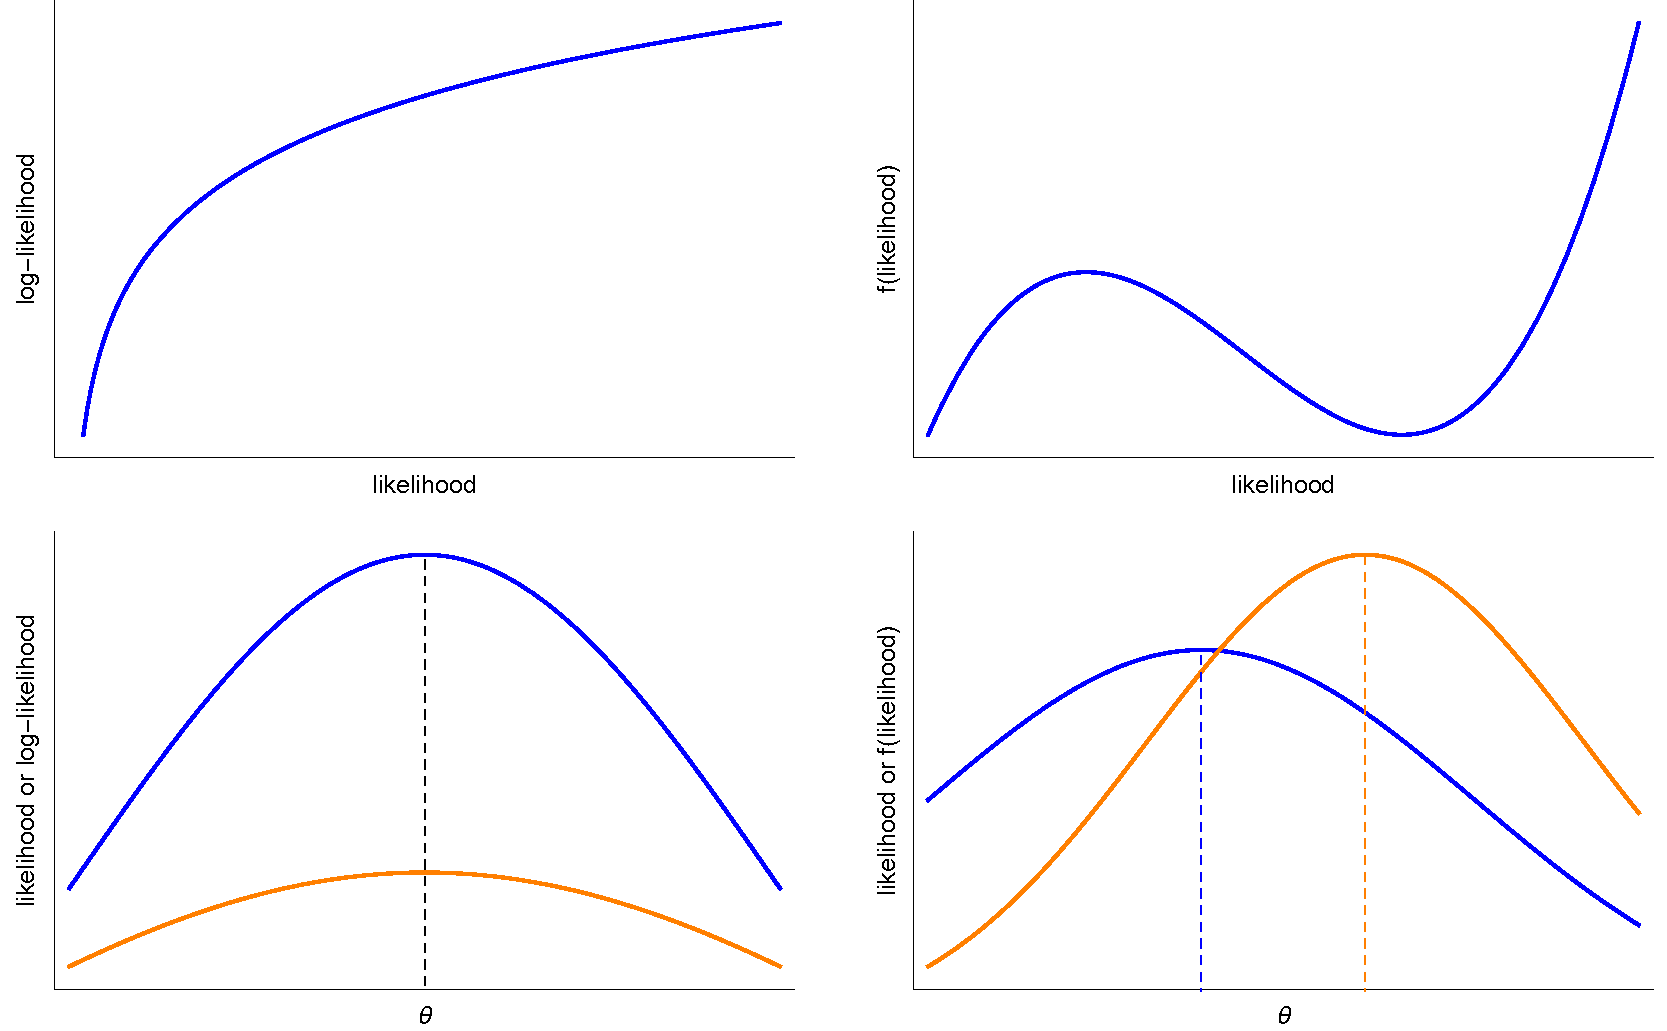
\includegraphics{Likelihood_logMonotonicity.pdf}}
\caption{The monotonicity of log-likelihood (top-left), means that the peaks of likelihood and log-likelihood coincide (bottom-left). However, this is not the case for an arbitrary function (top-right and bottom-right).\textbf{Add legends to the bottom two graphs.} }\label{fig:Likelihood_logMonotonicity}
\end{figure}

Remember, that since we are varying $\theta$ and holding the data constant here, that (\ref{eq:Likelihood_binomialNew}) is a \textit{likelihood}, not a probability. We then need to simply choose $\theta$ so that we can maximise the likelihood. We could simply differentiate (\ref{eq:Likelihood_binomialNew}) as it stands, and set the derivative equal to 0; rearranging the resultant equation for $\theta$. However, to make life a little easier for us, we are first going to take the \textit{log} of this expression, then differentiate it, setting the derivative to 0; resulting in the same value of $\theta$. We are able to do this because of the simple properties of the log transformation (see figure \ref{fig:Likelihood_logMonotonicity}):

\begin{equation}\label{eq:Likelihood_logLikelihoodBinomial}
l(\theta|data) = Log \left(L(\theta|data)\right) = log{100 \choose 10}+ 10log(\theta)+ 90 log(1-\theta)
\end{equation}

Where to get the result (\ref{eq:Likelihood_logLikelihoodBinomial}), we have used the log rules:

\begin{align}\label{eq:Likelihood_logRules}
log(ab) &= log(a) + log(b)\\
log(a^b) &= blog(a)
\end{align}

We can now simply differentiate the log-likelihood $l(\theta|data)$:

\begin{equation}\label{eq:Likelihood_binomialderiv}
\frac{\partial l}{\partial \theta} = \frac{10}{\hat{\theta}}-\frac{90}{1-\hat{\theta}} = 0
\end{equation}

If we set the derivative to 0 we then obtain the maximum likelihood \textit{estimate}, $\hat{\theta} = \frac{1}{10}$ (see figure \ref{fig:Likelihood_MLE}).

\begin{figure}
\centering
\scalebox{0.75} 
{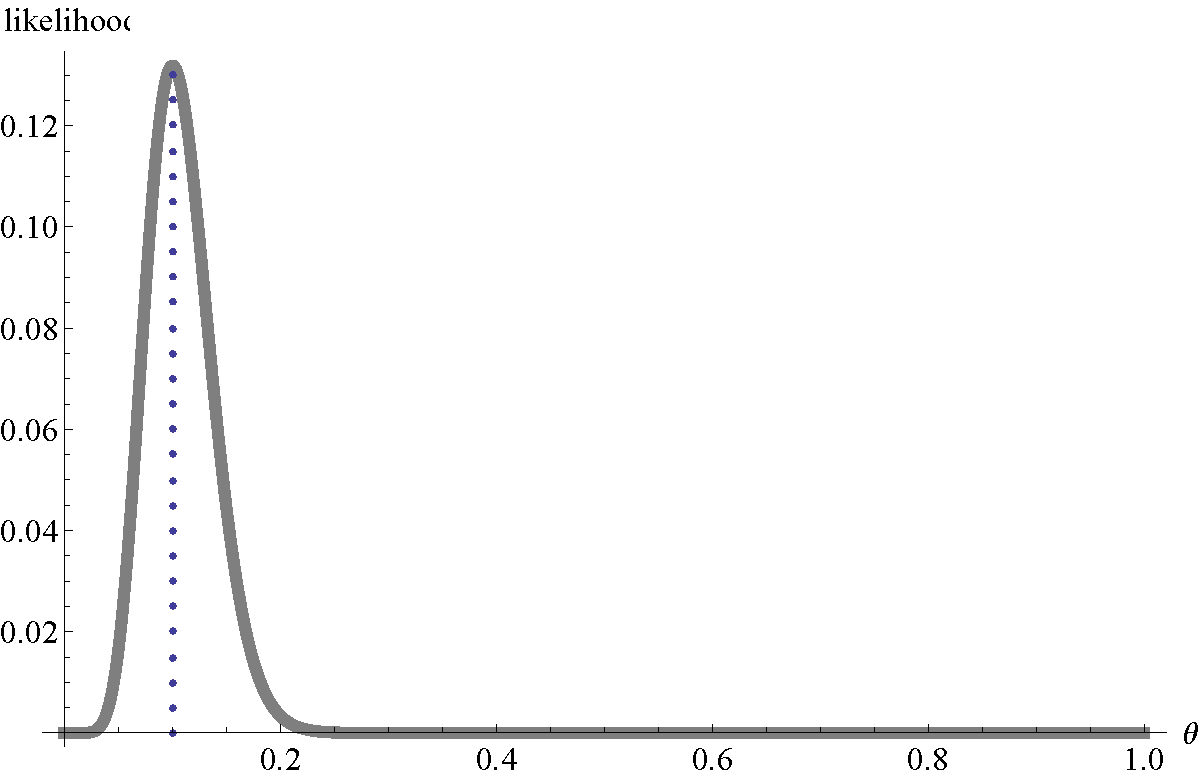
\includegraphics{Likelihood_ML.pdf}}
\caption{Log-likelihood of disease prevalence from section \ref{sec:Likelihood_diseaseMLE} as a function of the proportion of individuals which have the disease in a population, $\theta$. The dotted line shows the maximum likelihood estimate $\hat{\theta}=1/10$.}\label{fig:Likelihood_MLE}
\end{figure}


This estimator makes sense intuitively. The value of the parameter which results in the highest likelihood of obtaining the data occurs when the population prevalence exactly matches that obtained in our sample. In general if we found a number $\beta$ of individuals out of a sample of size $N$, who were disease-positive, then we would again find that the preceding analysis results in an estimator\footnote{An estimator is a mathematical function which outputs an estimate of a parameter in our model.} of the disease prevalence exactly equal to that in our sample:

\begin{equation}\label{eq:Likelihood_binomialestimator}
\hat{\theta} = \frac{\beta}{N}
\end{equation}

\subsection{Estimating the mean and variance in intelligence scores}
We are given a sample of individuals with test scores $\{75,71\}$, and we model the test scores using a normal likelihood as described in section \ref{sec:Likelihood_normal}:

\begin{equation}\label{eq:Likelihood_normalTwo}
L(\mu,\sigma^2|X_1=75,X_2 =71) = \frac{1}{\sqrt{2\pi\sigma^2}}e^{-\frac{(75-\mu)^2}{2\sigma^2}}\times \frac{1}{\sqrt{2\pi\sigma^2}}e^{-\frac{(71-\mu)^2}{2\sigma^2}}
\end{equation}

We can then proceed as we did in section \ref{sec:Likelihood_diseaseMLE} by taking the log of this expression before we differentiate it:

\begin{equation}\label{eq:Likelihood_diseaseLogLikelihood}
l(\mu,\sigma^2|X_1=75,X_2 =71) = 2log\left(\frac{1}{\sqrt{2\pi\sigma^2}}\right)-{\frac{(75-\mu)^2}{2\sigma^2}}-{\frac{(71-\mu)^2}{2\sigma^2}}
\end{equation}

Where we have again used the log rules in (\ref{eq:Likelihood_logRules}) to achieve (\ref{eq:Likelihood_diseaseLogLikelihood}). We can now proceed to differentiate (\ref{eq:Likelihood_diseaseLogLikelihood}) with respect to both variables, holding the other constant, setting each to 0:

\begin{align}\label{eq:Likelihood_diseaseDerivativeOne}
\frac{\partial l}{\partial \mu} &= {\frac{(75-\hat{\mu})}{\hat{\sigma^2}}}+{\frac{(71-\hat{\mu})}{\hat{\sigma^2}}} = 0\\
\frac{\partial l}{\partial \sigma^2} &= -\frac{1}{\hat{\sigma^2}} + \frac{(75-\hat{\mu})^2+(71-\hat{\mu})^2}{2\hat{\sigma^4}} = 0
\end{align}

The first of these expressions yields $\hat{\mu} = \frac{71+75}{2} = 73$, which when put into the second gives: 

\begin{equation}
\hat{\sigma^2} = \frac{1}{2}\left[(75-73)^2 + (71-73)^2)\right] = 4
\end{equation}

Note that technically, when we find the parameter values corresponding to the maximum likelihood we should check that we have not achieved a minimum (since this will also have a zero gradient). We could do this either by graphing the likelihood, or by checking that the second derivative is negative.

Notice that the maximum likelihood estimators for the population mean and variance are for this case the \textit{sample mean} and \textit{sample variance}\footnote{Albeit a biased estimator of the population variance. The unbiased estimator would divide by 1, rather than 2.}. In fact, this holds for the case of N individuals' data, then the maximum likelihood estimators for this case would be:

\begin{equation}
\hat{\mu} = \frac{1}{N}\sum\limits_{i=1}^{N} X_i = \bar{X}
\end{equation}
\begin{equation}
\hat{\sigma^2} = \frac{1}{N}\sum\limits_{i=1}^{N}(X_i-\bar{X})^2 = s^2
\end{equation}

\subsection{Maximum likelihood in simple steps}
In the above examples we note that we follow the same procedure to arrive at maximum likelihood estimates of parameters. Here, for clarity and as a recap, we note down these steps:

\begin{enumerate}
\item Find the density of a single data point.
\item Create the joint density.
\item Change perspective from a probability density, to a \textit{likelihood} (assume that the data is fixed, and the parameters vary).
\item Take the log of the joint density.
\item Maximise the log-likelihood.
\item (Check that it is a maximum, either graphically or by sign of second derivative).
\end{enumerate}

\section{Frequentist inference in Maximum Likelihood}\label{sec:Likelihood_maxlikelihoodInference}
We have now detailed how to derive point estimates of parameters using the method of maximum likelihood. However, at the moment we are unable to make any conclusions about the population. This is because we do not have any idea as to whether we obtained a particular estimate of a parameter due to picking a weird sample, or because it \textit{actually} has a value in the population which is at this value. Frequentists get round this by examining a graph of log-likelihood near the maximum likelihood point estimate (see figure \ref{fig:Likelihood_likelihoodCurvature}). If the log-likelihood is strongly peaked near the maximum likelihood estimate, then this suggests that only a small range of parameters would yield a similar valued likelihood. By contrast, if the log-likelihood is gently peaked near the maximum likelihood estimate, then it is feasible that a large range of parameters would yield estimates close to this value. In the latter case, it seems logical that we should be less confident in the particular value of the parameter which is given by maximum likelihood. We can measure the 'peakedness' in the log-likelihood by looking at the magnitude of the second derivative\footnote{The first derivative gives the gradient, the second derivative gives the rate of change of the gradient - a measure of curvature.} of the function at the maximum likelihood point estimate value. The more curved the log-likelihood, the more confident we can be of our estimated parameter value, and any conclusions drawn from this. Note however, that the Frequentist inference is not based on proper probability distributions (since we infer based on a likelihood). This contrasts with the Bayesian method which, by its nature, allows for a more adequate description of parameters, using probability distributions.

\begin{figure}
\centering
\scalebox{0.65} 
{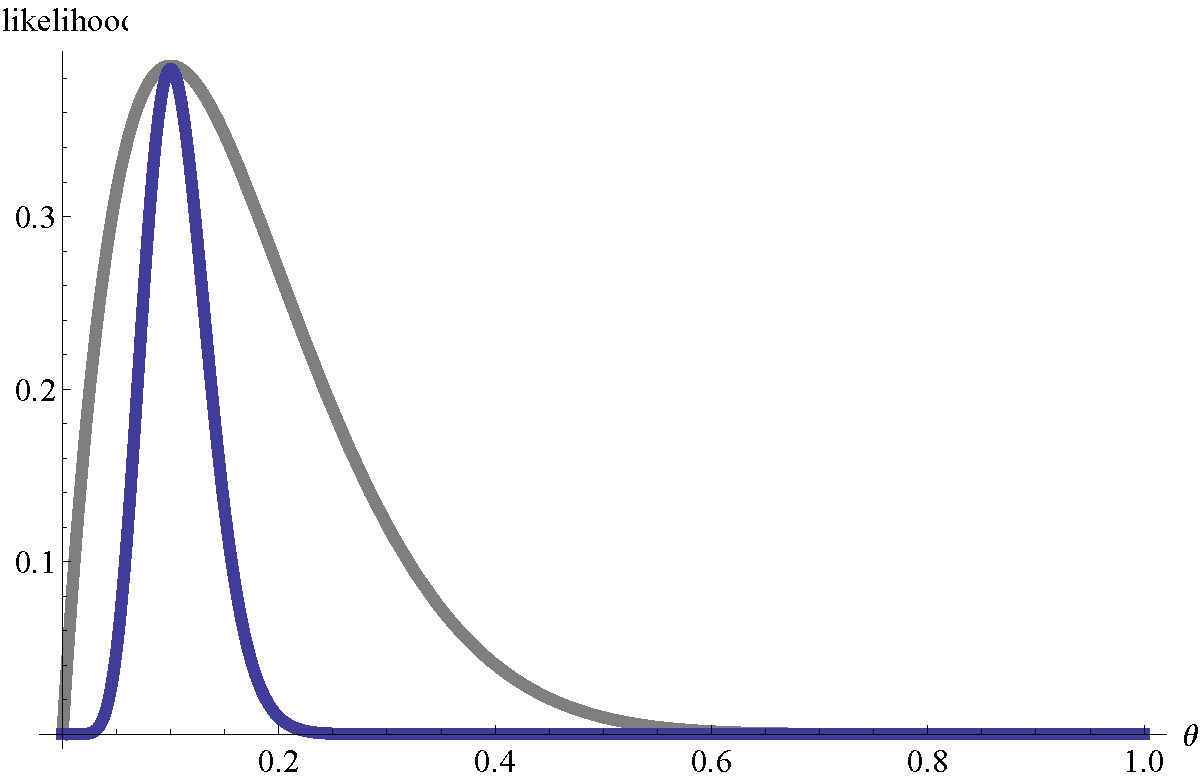
\includegraphics{Likelihood_likelihoodCurvature.pdf}}
\caption{Two likelihoods which result in the same maximum likelihood estimates of parameters, at 0.1. The gray likelihood is less strongly-peaked, meaning we can be less confident about the estimates.}\label{fig:Likelihood_likelihoodCurvature}
\end{figure}


\section{Chapter summary}
We should now understand what is meant by a likelihood, and how to build probabilistic models of real life processes. However, the difficulty of modelling a process is governed by its degree of complexity and sensitivity to violations of assumptions. Further we should also understand how the Frequentist method of Maximum Likelihood can be used to yield point estimates of parameters. We are however, currently restricted in our ability to make inferences based on full probability distributions over parameters. Bayes' rule tells us how we can convert a likelihood - itself not a proper probability distribution - to a posterior (\textit{correct}) probability distribution for parameters. In order to use to do this though, we need to understand what is meant by a \textit{prior} distribution and how we can specify this distribution to suit the particular situation. This is what is covered in the next chapter.

\section{Chapter outcomes}
The reader should now be familiar with the following concepts:

\begin{enumerate}
\item The difference between likelihoods and probabilities.
\item The need for probabilistic models in some circumstances.
\item How to go about choosing an appropriate likelihood for a given situation.
\item The exchangeability assumption.
\item Maximum likelihood, and how to carry out inference in this framework.
\end{enumerate}

\section{Problem set}
\subsection{Blog blues.}
We suppose that visits to your newly-launched blog occur sporadically. Suppose you were interested in the length of time between consecutive first-time visits to your homepage. You collect the time data for a given 100 visits to your blog for a particular time period and day, and you set about thinking about building a statistical model.
\subsubsection{What assumptions might you make about the first-time visits?}
\subsubsection{What model might be appropriate to model the time between visits?}
\subsubsection{Algebraically derive an estimate of the mean number of visits per hour}
\subsubsection{Data analysis:} you collect time data from Google Analytics\footnote{A popular provider of website analytics data.} for 1000 visits. The data set is called XXXX. \textbf{Derive an estimate of the mean number of visits per hour.}
\subsubsection{Graph the log likelihood near your estimated value. What does this show? Why don't we plot the likelihood?}
\subsubsection{Estimate confidence intervals around your parameter.}
\subsubsection{What is the probability that you will wait:}
\begin{enumerate}
\item 1 minutes or more.
\item 5 minutes or more.
\item Half an hour or more.
\end{enumerate}
before your next visit?
\subsubsection{Evaluate your model.}
\subsubsection{What alternative models might be useful here?}
\subsubsection{What are the assumptions behind these models?}
\subsubsection{Estimate the parameters of your new model.}
\subsubsection{Use your new model to estimate the probability that you will wait:}
\begin{enumerate}
\item 5 minutes.
\item 20 minutes.
\item 1 hour.
\end{enumerate}
before your next visit?

\subsubsection{Hints: the exponential is to the poisson model, what the ? is to the negative binomial.}

\subsection{Violent crime counts in New York counties}
In data file XXX we have compiled a data set of the population, violent crime count and unemployment across New York counties in 2014. 

\subsubsection{Graph the violent crime account against population. What type of relationship does this suggest?}
\subsubsection{A simple model}
A simple model here might be to assume that the crime count in a particular county is related to the population size by a poisson model:
\begin{equation}
crime_i \sim poisson(n_i\theta)
\end{equation}
\subsubsection{What are the assumptions of this model?}
\subsubsection{Estimate the parameter $\theta$ from the data. What does this parameter represent?}
\subsubsection{Do these assumptions seem realistic?}
\subsubsection{Estimate a measure of uncertainty in your estimates.}
\subsubsection{Evaluate the performance of your model.}

\subsubsection{A better model}
An alternative model allows each county to be heterogeneous with respect to its susceptibility to crime, and has a specification of the form:
\begin{equation}
crime_i \sim poisson(n_i\theta_i)
\end{equation}
\subsubsection{Why is this model better?}
\subsubsection{What factors might affect $\theta_i$?}
\subsubsection{Write down a new model specification taking into account the previous point.}
\subsubsection{Estimate the parameters of this new specification.}
\subsubsection{How does this new model compare to the previous iteration?}
\subsubsection{What alternative specifications might be worth attempting?}

\subsection{Monte Carlo evaluation of the performance of MLE in R}
Ben to add later.

\subsection{The sample mean as MLE}
Ben to add later.

\chapter{Priors}\label{chap:Prior}
\section{Chapter Mission statement}
At the end of this chapter a reader will know what is meant by a prior, and the different philosophies that are used to understand and construct them. 

Insert a graphic with the likelihood part of Bayes' formula circled, as in the equation shown below for the part highlighted in blue.

\begin{equation}
p(\theta|data) = \frac{p(data|\theta)\times {\color{blue}p(\theta)}}{p(data)}
\end{equation}\label{eq:Prior_BayesHighlighted}

\section{Chapter goals}
Bayes' rule tells us how to convert a likelihood - itself not a proper probability distribution - into a posterior probability distribution for parameters, which can then be used for inference. We are required in the numerator to multiply the likelihood by a pre-experimental weighting of each set of parameter values described by a probability distribution, which is known as a \textit{prior}. Priors are without doubt the most controversial aspect of Bayesian statistics, with opponents criticising its inherent \textit{subjectivity}. It is hoped that by the end of the chapter we will have convinced the reader that, not only is subjectivity inherent in \textit{all} statistical models - both Frequentist and Bayesian - but the explicit subjectivity of priors is more transparent, and hence open to interrogation, than the implicit subjectivity abound elsewhere.

This chapter will also explain the differing interpretations which are ascribed to priors. The reader will come to understand the types of method that can be used to construct prior distributions, and how they can be chosen to be minimally subjective, or otherwise to contain informative pre-experimental insights from data or opinion. Finally, the reader will understand that if significant data are available then the conclusions drawn should be insensitive to the initial choice of prior.

Inevitably, this chapter will be slightly more philosophical and abstract than other parts of this book, but it is hoped that the examples given will be sufficient to ensure its practical use.

\section{What are priors, and what do they represent?}
Chapter \ref{chap:Likelihoods} introduced us to the concept of formulating a likelihood, and how this can be used to derive Frequentist estimates of parameters, using the method of maximum likelihood. This pre-supposes that the parameters in question are immutable, fixed quantities that actually exist, and can be estimated by methods that can be repeated, or imagined to be repeated many times \cite{gill2007bayesian}. As Gill (2007) indicates, this is unrealistic for the vast majority of social science research.

\begin{quotation}
It is simply not possible to rerun elections, repeat surveys under exactly the same conditions, replay the stock market with exactly matching market forces, or re-expose clinical subjects to identical stimuli.
\end{quotation}

Furthermore, parameters only exist because we have \textit{invented} a model, hence we should innately be suspicious of any analysis which assumes an existence of a single certain value for any aspect of these abstractions.

For Bayesians, it is the data that are treated as fixed, and the parameters that vary. We know that the likelhood - however useful - is not a proper probability distribution. Bayes' rule tells us how to combine a likelihood with something called a \textit{prior} to obtain a proper posterior distribution for the parameter in question, which can then be used for inference. But what does it actually mean for a parameter to have a prior distribution?

Gelman et al. (2013) suggests that there are two different interpretations of priors: the \textit{state of knowledge} interpretation, where we specify our knowledge and uncertainty in a parameter as if regarding it as a draw from a probability distribution; alternatively in the more objective \textit{population} interpretation where the current value of a parameter is the result of a draw from a true population distribution \cite{gelman2013bayesian}. In both viewpoints the model parameters are not viewed as static, unwavering constants as they are taken to be in Frequentist theory.

\begin{figure}
\centering
\scalebox{0.3} 
{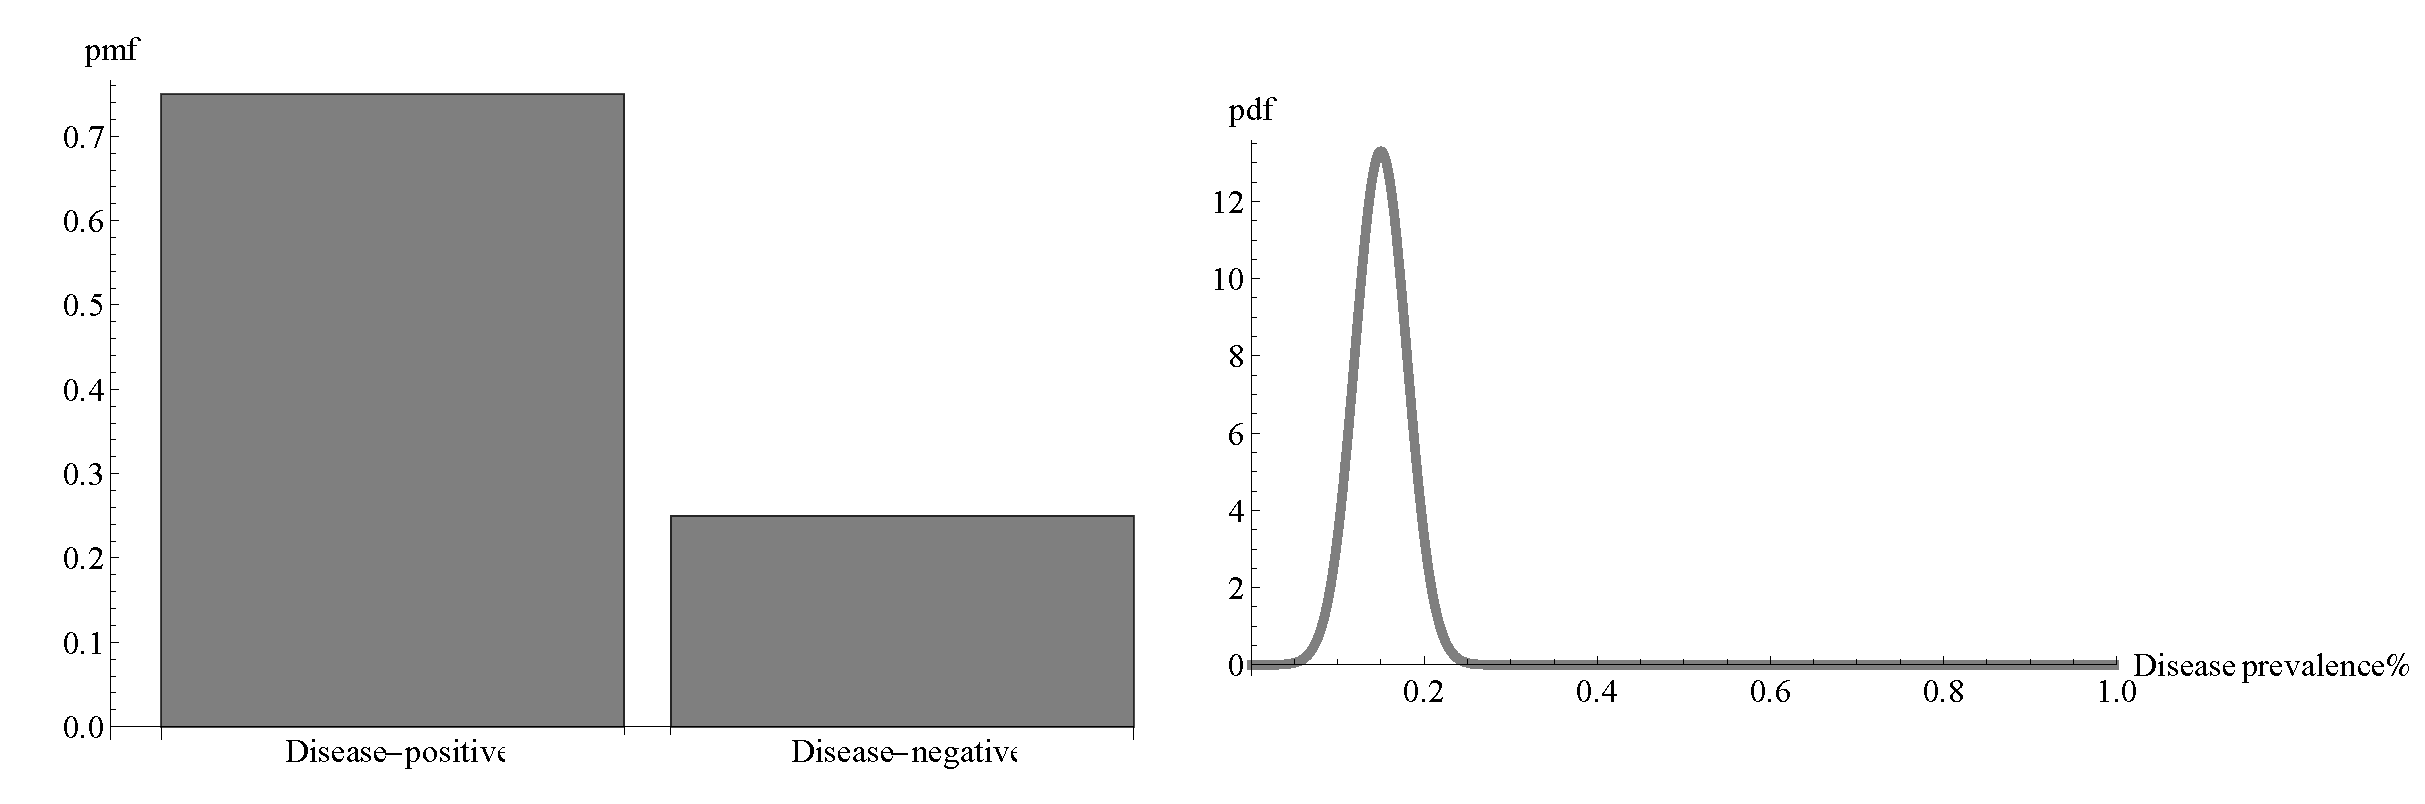
\includegraphics{Prior_introduction.pdf}}
\caption{Left - a prior for a doctor's pre-testing diagnostic probability of an individual having a disease. Right - a prior which represents pre-sample uncertainty in disease prevalence.}\label{fig:Prior_introduction}
\end{figure}

If we adopt the \textit{subjective} state of knowledge viewpoint above, then we can think of the prior as representing our pre-experimental/data certainty in the parameter in question. For example, imagine that a Doctor is asked to evaluate the probability that a given individual has a particular disease, before the results of a blood test become available. Using their knowledge of the patient's history and their expertise on the particular condition, they assign a prior disease probability of 75\% (see figure \ref{fig:Prior_introduction}). 

Alternatively, imagine we are tasked with estimating the proportion of the UK population that has this disease. We may have some idea of its prevalence, as well as the variance in the mean prevalence of a disease across a range of previous samples of individuals which have been tested. In this case, the prior is continuous and represents our uncertainty in our estimate of the prevalence (see figure \ref{fig:Prior_introduction}). 

In all cases a prior is a proper probability distribution, and hence can be used to elicit our prior expectations as to the value of a parameter. For example, we could use the prior probability distribution for the proportion of individuals having a particular disorder in figure \ref{fig:Prior_introduction} to estimate a pre-experimental mean of approximately 15\% prevalence. 

Adopting the \textit{population} perspective, we imagine the value of a parameter of current interest to be drawn from a population distribution. If we imagine the process of flipping a coin, we could if we knew the angle at which it is tossed, as well as the height from which it is thrown above the surface\footnote{Also assuming that we knew the physical properties of the coin and surface.} predict deterministically the side on which the coin would fall face up. We could then hypothetically enumerate the (infinitely) many angles and heights of the coin, and for each set determine whether the coin would fall face up or down. Each time we throw the coin we are implicitly choosing an angle and height from the set of all possible combinations, which determines whether a heads or tails falls face up. Some ranges of the angle and the height will be more frequently chosen than others, albeit relatively agnostic with regards to final state of the coin.  Hence we could think of this choice as the realisation from a distribution of all possible sets. Thus we could think about the choice of angle and height as being a realisation from this \textit{population} distribution, and hence determines the fate of the coin toss.

\boxed{Interactive:} see the interactive tool XXX which allows you to investigate the population interpretation of priors for local literacy rates in the US. 

Alternatively, going back to the disease prevalence example, we could imagine that each time we pick a sample, the data we obtain is partly determined by the exact characteristics of the sub-populations from which these individuals were drawn. The other part of variability is sampling variation within those sub-populations. Here we can view the particular sub-population characteristics as draws from an overall population distribution of parameters, representing the entirety of the UK. 

\section{Why do we need priors at all?}
A question we might ask is, why do we need priors at all? Can't we simply let the data speak for itself, without the need of these subjective beasts? 

Frequentists without knowing it actually do use something equivalent to priors, by setting the size of statistical tests\footnote{See section \ref{sec:Intro_implicitExplicitSubjectivity} for a further discussion.}. However, can't we as Bayesians side-step this subjective jump completely?

The answer to this question is provided by Bayes' rule. Its inclusion in Bayes' rule, which is the only correct way to update beliefs, means that if we are to be consistent with the laws of probability, we are required to provide this part for any Bayesian inferential procedure. 

If you find this description somewhat unsatisfying, then another way of re-phrasing this argument, is that Bayes' rule is really only a way to \textit{update} our initial beliefs, to yield new beliefs which reflect the weight of the data obtained:

\begin{equation}
initial\; belief \xrightarrow{Bayes' rule} new\;beliefs
\end{equation}

Viewed in this light, it is clear that we need to specify an initial belief, otherwise we have nothing to update! Bayes unfortunately doesn't tell us how to formulate this initial belief, but fear not, in this chapter we will delve into how we can go about setting priors in practice.

\section{Why don't we just normalise likelihood by choosing a unity prior?}\label{sec:Prior_unityPrior}
Another question that can be asked is, 'Why can't we simply let the prior be the same for all values of $\theta$?'; in other words set $p(\theta) = 1$ in the numerator of Bayes' rule; resulting in a posterior that takes the form of a normalised likelihood:

\begin{equation}
p(\theta|data) = \frac{p(data|\theta)} {p(data)}
\end{equation}\label{eq:Prior_BayesNormalisedLikelihood}


This would surely negate the need for specification of a prior, and thwart all attempts to denounce Bayesian statistics as \textit{subjective}. So why don't we do just that? 

There is a pedantic, mathematical argument against this, which is that $p(\theta)$ must be a proper probability distribution to ensure the same properness of the posterior. If we choose $p(\theta) = 1$ (or in fact any positive constant), then the integral $\int\limits_{-\infty}^{+\infty}p(\theta)\mathrm{d}\theta\rightarrow\infty$, and we can no longer think of the distribution, $p(\theta)$ as representing a probability distribution. It may still be possible that even if the prior is improper, that the resultant posterior also satisfies the required properties of a proper probability distribution, but care must be taken when using these distributions for inference, as technically they are \textit{not} probability distributions, due to the abuse of Bayes' rule. In this case the posteriors can only be viewed, at best, as approximations to the result we would have obtained under some limiting prior distribution.

Another, perhaps more persuasive argument, is that by assuming all parameter sets have an equal likelihood of being chosen beforehand, then this can result in nonsensical resultant conclusions being drawn. Consider the following example: 

We are given some data on a coin which has been flipped twice, with the result $\{H,H\}$. We are given the choice of deciding whether the  coin is fair, with an equal chance of both heads and tails occurring, or biased with a very strong weighting towards heads. We denote fairness by a parameter $\theta=1$, if the coin is fair, and $\theta=0$ otherwise.

\begin{figure}
\centering
\scalebox{0.1} 
{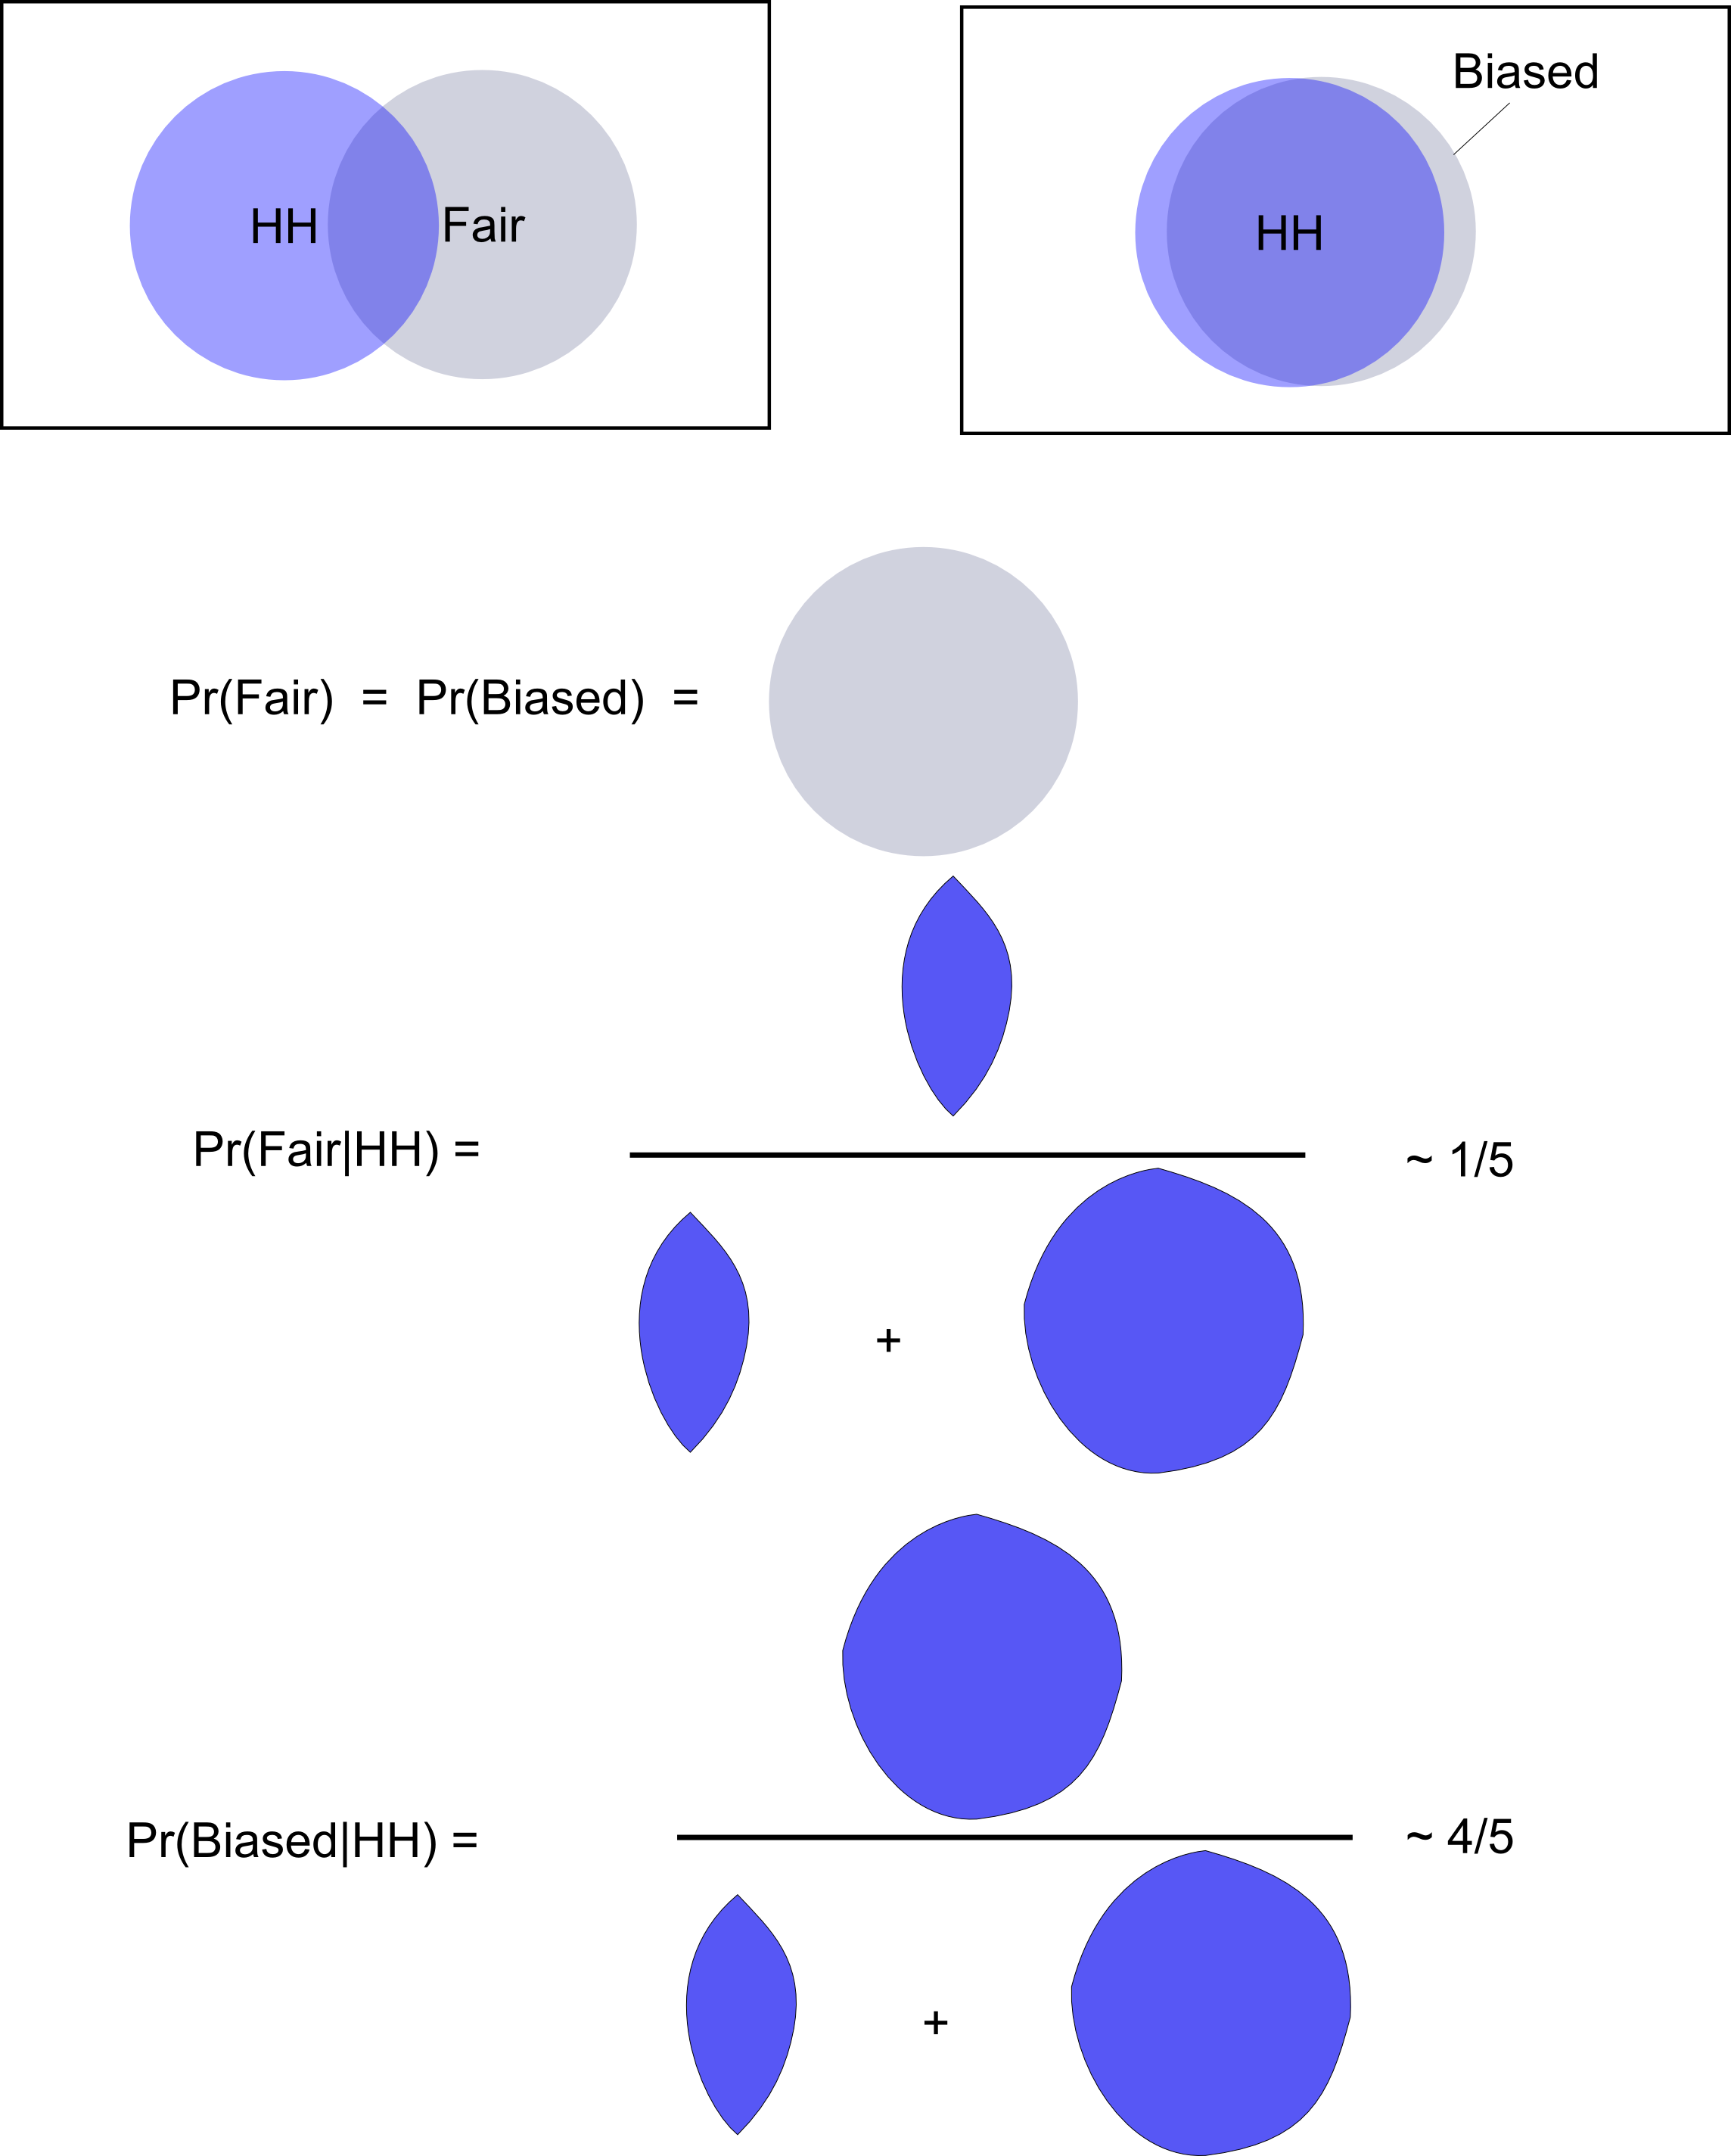
\includegraphics{Prior_priorJustificationCoin.png}}
\caption{The top two boxes represent the different world views for left: the coin being fair, and right: the coin being biased. If we suppose that these two views have the same prior probability, illustrated here by them having the same area, then use of Bayes' rule means that we suppose the coin is likely bias.}\label{fig:Prior_priorJustificationCoin}
\end{figure}

Figure \ref{fig:Prior_priorJustificationCoin} illustrates how assuming a uniform prior in this case results in a very strong posterior weighting towards the coin being biased. This is because from a likelihood perspective - $p(data|\theta)$ - if we assume that the coin is biased, then the probability of obtaining two heads is high. Whereas if we assume that the coin is fair, then the probability of obtaining this data is only $\frac{1}{4}$. Thus, by ignoring common sense - that it is likely the majority of coins are relatively unbiased - we end up with a result that is nonsensical. 

\boxed{Interactive:} see the interactive tool XXX which allows you to play around with your prior probability of a coin being biased, and note its effect on the posterior.

Of course, in this example we would hope that by collecting more data, in this case, throws of the coin, we could be confident in the conclusions drawn from the likelihood. However, Bayesian analysis allows us to achieve such a goal with a smaller sample size, should we be relatively confident about our pre-data knowledge.

\section{The explicit subjectivity of priors}
Opponents of Bayesian approaches to inference criticise the subjectivity inherent with choice of prior. However, all analysis involves a degree of subjectivity, particularly in regard to choice of statistical model. This choice is often formulated implicitly as being \textit{objectively} correct, with little justification or discourse given to the underlying assumptions necessary to arrive there. The statement of a prior, necessary for any full description of a Bayesian analysis, is at least \textit{explicit}; leaving this aspect of the modelling subject to the same interrogation and academic examination to which any analysis should be subjected. A word that is often used by protagonists of Bayesian methods, is that it is \textit{honest} due to the \textit{explicit} statement of assumptions. The statement of pre-experimental biases actually forces the analyst to self-examine, and perhaps also leads to a decline in the temptation to manipulate the analysis to one's own ends.

\section{Combining a prior and likelihood to form a posterior} 
This chapter thus far has given more attention to the philosophical and theoretical underpinnings of Bayesian analysis. Now we change tack to illustrate to the reader the mechanics behind Bayes' formula; specifically how the prior is combined with the likelihood to yield a posterior probability distribution. The following examples introduce an illustrative method, known as \textit{Bayes' box} described in detail in \cite{stewart2014teaching} and \cite{bolstad2007introduction}, which illustrates the functioning of Bayes' rule, in which the parameter, prior, likelihood, and posterior are all displayed in a logical manner.

\subsection{The Goldfish game}\label{sec:Prior_urn}
Imagine a covered bowl of water, containing 5 fish, each of which is red or white, and suppose we are tasked with inferring the total number of red fish which are present in the bowl, on the basis of a single fish which we pick out, and find to be red. Before we pull the fish out from the bowl, we have no prejudice for a particular number of red fish, and so suppose that all possibilities - 0 to 5 - are equally likely, and hence have the probability of $\frac{1}{6}$ in our discrete prior. Our model for the likelihood is that a number $Y$ of the fish are red, and that the result of an individual picking a fish from the bowl tells us nothing about future picks, apart from their joint dependence on $Y$. In this oversimplified example, this independence assumption seems reasonable, particularly if the fish are picked out in a randomised manner and have no distinguishing features. Further suppose that the random variable $X\in\{0,1\}$ indicates whether a fish is white or red respectively.  The analogy with the disease status of an individual described in section \ref{sec:Likelihood_individualDisease} is evident, and hence we choose a likelihood of picking a red fish of the form:

\begin{equation}\label{eq:Prior_bernoulli}
P(X = 1|Y=\alpha) = \frac{\alpha}{5}
\end{equation}

In (\ref{eq:Prior_bernoulli}), $\alpha\in\{0,1,2,3,4,5\}$ represents the number of red fish in the bowl.

We can then illustrate the functioning of Bayes' rule in the \textit{Bayes' box} shown in table \ref{tab:Prior_bayesBoxDiscreteUrns}. We start by listing all the possible numbers of red fish that can exist in the bowl in the leftmost column. We then introduce our prior probabilities that we associate with each of the six potential numbers of red fish that can be in the bowl. In the third column we then calculate the likelihoods for each of the outcomes using the simple rule given in (\ref{eq:Prior_bernoulli}). We then multiply the prior by the likelihood in the fourth column, which on summation gives us $p(data)=\frac{1}{2}$, which we use to create a proper probability distribution for the posterior in the last column. For a mathematical description of this process see section \ref{app:Prior_bayesUrn}.

The Bayes' box illustrates the straightforward and mechanical working of Bayes' rule for the case of discrete data. We also note that when we sum the likelihood over all possible numbers of red fish in the bowl - in this case the parameter which we are trying to infer - we find this to be equal to 3; illustrating again that a likelihood is not a valid probability distribution. We also see that at a particular parameter value, if either the prior or the likelihood are found to be zero as is the case of 0 red fish being in the urn (impossible since we have at least one), then this ensures that the posterior distribution is zero at this point. This makes it important that we use a prior that gives a positive weight to \textit{all} possible ranges of parameter values. The results are also displayed graphically in figure \ref{fig:Prior_urnStacked}.

\begin{table}[htbp]
  \centering
  \caption{A Bayes' box showing how to calculate the posterior for the case of drawing fish from a bowl containing a 5 fish mixture of red and white fish, one of which has been drawn and shown to be red. Here we assume that pre-experiment all possible numbers of red fish are equally likely, by adopting a uniform prior.}\label{tab:Prior_bayesBoxDiscreteUrns}
    \begin{tabular}{ccccc}
    \toprule
    \textbf{Number of red fish} & \textbf{Prior} & \textbf{Likelihood} & \textbf{Prior x likelihood} & \textbf{Posterior$=\frac{Prior\times Likelihood}{p(data)}$} \\
    \midrule
    0     &  1/6  & 0     & 0       & 0       \\
    1     &  1/6  &  1/5  &   1/30 &   1/15 \\
    2     &  1/6  &  2/5  &   1/15 &   2/15 \\
    3     &  1/6  &  3/5  &   1/10 &   3/15  \\
    4     &  1/6  &  4/5  &   2/15 &   4/15 \\
    5     &  1/6  & 1     &   1/6  &   5/15  \\
    \bottomrule
    Total & \textbf{1    } & \textbf{3    } & \textbf{$p(data)=1/2$ } & \textbf{1      } \\
    \bottomrule
    \end{tabular}%
  \label{tab:addlabel}%
\end{table}%

\begin{figure}
\centering
\scalebox{0.75} 
{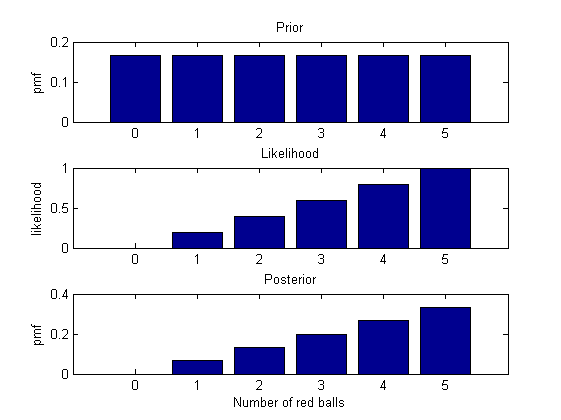
\includegraphics{Prior_urnStacked.png}}
\caption{The prior, likelihood and posterior for the fish example described in \ref{sec:Prior_urn}. The prior in the upper panel gives uniform weighting to all possible numbers of red fish. This is then multiplied by the likelihood (in the middle panel) at each number of fish, and normalised to make the posterior density shown in the bottom panel.}\label{fig:Prior_urnStacked}
\end{figure}

Now suppose that we had reason to believe that the game-maker had a prejudice towards more equal numbers of both fish, and as a result we alter our prior to have a greater weight towards these numbers of red fish(see table \ref{tab:Prior_bayesBoxUrnUpdated} and figure \ref{fig:Prior_bayesUrnUpdated}).


\begin{table}[htbp]
  \centering
  \caption{A Bayes' box showing how to calculate the posterior for the case of drawing fish from a bowl containing a 5 fish mixture of red and white fish, one of which has been drawn and shown to be red. Here we assume that pre-experiment all possible numbers of red fish are equally likely, by adopting a uniform prior.}\label{tab:Prior_bayesBoxUrnUpdated}%
    \begin{tabular}{ccccc}
    \toprule
    \textbf{Number of red fish} & \textbf{Prior} & \textbf{Likelihood} & \textbf{Prior x likelihood} & \textbf{Posterior$=\frac{Prior\times Likelihood}{p(data)}$} \\
    \midrule
    0     &   1/12 & 0     & 0       & 0       \\
    1     &   1/6  &  1/5  &   1/30 &   1/15 \\
    2     &   1/4  &  2/5  &   1/10 &   1/5  \\
    3     &   1/4  &  3/5  &   3/20 &   3/10 \\
    4     &   1/6  &  4/5  &   2/15 &   4/15 \\
    5     &   1/12 & 1     &   1/12 &   1/6  \\
    \bottomrule
    Total & \textbf{1      } & \textbf{3    } & \textbf{  1/2 } & \textbf{1      } \\
    \bottomrule
    \end{tabular}%
  
\end{table}%

\begin{figure}
\centering
\scalebox{0.75} 
{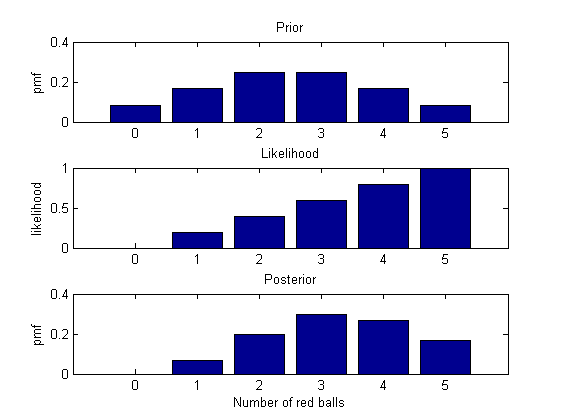
\includegraphics{Prior_bayesUrnUpdated.png}}\caption{The prior, likelihood and posterior for the goldfish game example described in \ref{sec:Prior_urn}. The prior in the upper panel gives more weighting to more equal numbers of red and white fish. This is then multiplied by the likelihood (in the middle panel) at each number of fish, and normalised to make the posterior density shown in the bottom panel.}\label{fig:Prior_bayesUrnUpdated}
\end{figure}


\boxed{Interactive:} see the interactive tool XXX to play the goldfish game!

\subsection{Disease proportions revisited}\label{sec:Prior_diseaseProp}
Suppose that we substitute our goldfish bowl from section \ref{sec:Prior_urn} for a sample of 100 individuals taken from the UK population. Suppose also that we continue to assert the independence of individuals within our sample, and make explicit the assumption that individuals are from the same population, and are hence identically-distributed. We are now interested in making conclusions about the overall proportion of individuals within the population who have the disease, $\theta$. Let's suppose that within a sample of 10 we find 3 of them who are disease-positive\footnote{We also suppose that there are no false-positives here.}. We could then use the assumptions of independence and identical-distribution to write down a likelihood of the form introduced in section \ref{sec:Likelihood_diseaseGroup}:

\begin{equation}\label{eq:Prior_binomial}
P(Z=3|\theta) = {10 \choose 3} \theta^\beta (1-\theta)^{10-3}
\end{equation}

The reason for the ${10 \choose 3}=120$ term at the beginning of (\ref{eq:Prior_binomial}) is that we have to count the number of different permutations of getting 3 individuals who are disease-positive within a sample size of 10. 

We suppose that at the beginning of the experiment all values of $\theta$ are equally likely. However, we would expect researchers to have a pre-experimental idea as to the most probable frequencies of the disease within the population, meaning that a flat prior which is given is likely understating a prejudice towards a certain range of $\theta$ values. Whilst, this is the case, it is often assumed in research papers - for the sake of objectivity - that priors are flat, in order to try to minimise the effect which assumptions here make on the outcome of an analysis.

Since the parameter of interest is now continuous, it would appear that we can't use Bayes' box here, as there would be infinitely many rows (corresponding to the continuum of possible $\theta$) over which to sum. However, we can still use it to approximate the shape of the posterior, if we discretise the prior and likelihood at 0.1 intervals across the [0,1] range for $\theta$ (see table \ref{tab:Prior_BayesDiscretised}). 

\begin{table}[htbp]
  \centering
    \begin{tabular}{ccccc}
    \toprule
    \textbf{$\theta$} & \textbf{Prior} & \textbf{Likelihood} & \textbf{Prior x likelihood} & \textbf{Posterior} \\
    \midrule
    0.00  & 0.09  & 0.00  & 0.00  & 0.00 \\
    0.10  & 0.09  & 0.06  & 0.01  & 0.07 \\
    0.20  & 0.09  & 0.20  & 0.02  & 0.22 \\
    0.30  & 0.09  & 0.27  & 0.02  & 0.30 \\
    0.40  & 0.09  & 0.21  & 0.02  & 0.23 \\
    0.50  & 0.09  & 0.12  & 0.01  & 0.13 \\
    0.60  & 0.09  & 0.04  & 0.00  & 0.04 \\
    0.70  & 0.09  & 0.01  & 0.00  & 0.01 \\
    0.80  & 0.09  & 0.00  & 0.00  & 0.00 \\
    0.90  & 0.09  & 0.00  & 0.00  & 0.00 \\
    1.00  & 0.09  & 0.00  & 0.00  & 0.00 \\
    \bottomrule
    \textbf{Total} & \textbf{1.00} & \textbf{0.91} & \textbf{p(data)=0.08} & \textbf{1.00} \\
    \bottomrule
    \end{tabular}%
  \caption{A Bayes box for the discretised disease example of section \ref{sec:Prior_diseaseProp}.}\label{tab:Prior_BayesDiscretised}%
\end{table}%

The method used to exactly posterior is identical to that which we see in the discretised Bayes' box of table \ref{tab:Prior_BayesDiscretised}, except now that we are multiplying two functions - one for the prior, the other for the likelihood. Essentially all we are doing is multiplying one set of values by another. We see here that the shape of the posterior is the same in both the discretised, as well as the true posterior (see figure \ref{fig:Prior_diseaseDiscretised}). The impact of using a flat prior here is that the posterior is peaked at the same value of $\theta$ as the likelihood. 

\boxed{Interactive:} See the following link to explore the effect of the prior, as well as the data sample, on the posterior for the disease proportions example.

\begin{figure}
\centering
\scalebox{0.5} 
{\includegraphics{Prior_diseaseDiscretised.pdf}}
\caption{The prior, likelihood and posterior for the \textbf{left:} discretised, and \textbf{right:} continuous disease proportion example described in section \ref{sec:Prior_diseaseProp}. Each point in $\theta$ along the continuous prior curve (top panel) is multiplied by the corresponding value of likelihood (middle panel), to form the numerator of Bayes' rule. The numerator is then normalised to make the posterior probability density shown in the bottom panel.}\label{fig:Prior_diseaseDiscretised}
\end{figure}

\section{Constructing priors}
There are a number of different methodologies and philosophies when it comes to the construction of a prior density. In this section we consider briefly how priors can be engineered so as to be relatively uninformative - better-termed vague - or alternatively can be used to assemble pre-experimental knowledge in a logical manner.

\subsection{Vague priors}\label{sec:Prior_vague}
When there is a premium placed on the objectivity of analysis, as is often the case in regulatory work - drug trials, public policy and the like - then use of a relatively 'uninformative' prior is often desired. If we were uncertain as to the proportion of individuals within a population who have a particular disease, then a uniform prior (see figure \ref{fig:Prior_jeffreysIntro}) is often employed to this end. 

The use of a prior that has a constant value, $p(\theta)=constant$, is attractive because in this case:

\begin{align}\label{eq:Prior_BayesFlatPrior}
p(\theta|data) &= \frac{p(\theta)\times p(data|\theta)}{p(data)}\\
& \propto p(\theta)\times p(data|\theta)\\
& \propto p(data|\theta)
\end{align}

In (\ref{eq:Prior_BayesFlatPrior}) we thus see that the shape of the posterior distribution is solely determined by the likelihood function. This is seen as a merit of uniform priors since they 'let the data speak for itself' through the likelihood. This is used as the justification for using a flat prior in many analyses.

The flatness of the uniform prior distribution is often termed 'uninformative', but this is misleading. If we assume the same model as described in section \ref{sec:Prior_diseaseProp}, then the probability that one individual has the disease is $\theta$, and the probability that two randomly sampled individuals both have the disease is $\theta^2$. If we assume a flat prior for $\theta$, then this implies a decreasing prior shown in figure \ref{fig:Prior_jeffreysIntro} for $\theta^2$. Furthermore, when we consider the probability that within a sample of ten individuals, all of whom are diseased, we see that a flat prior for $\theta$ implies an even more accentuated prior for this event; meaning that we beforehand give little weight to this event. For the mathematical details of these graphs see section \ref{app:Prior_diseaseJeffreys}.

\begin{figure}
\centering
\scalebox{0.75} 
{\includegraphics{Prior_jeffreysIntro.pdf}}\caption{The probability density for obtaining all diseased individuals within sample sizes of 1, 2 and 10 respectively. Starting out with a flat prior for the probability that one individual has a disease has resulted in non-flat priors for the other 2 probabilities.}\label{fig:Prior_jeffreysIntro}
\end{figure}

We can hence see that even though a uniform prior for an event looks, on first glances, to convey no information, we are actually making quite informative statements about other events. This aspect of choosing flat priors is swept under the carpet for most analyses, partly because often we care most about the particular parameter for which we create a prior. All priors contain some information, so we prefer the use of the terms "vague" or "diffuse" to represent situations where a premium is placed on drawing conclusions from only the data at hand.

\boxed{Interactive:} see the interactive tool XXX which allows you to select between different priors, and investigate their effect on the probability that a number of individuals have a disease.

There are methods for constructing priors that seek to limit the information contained within priors, so as to not colour the analysis with pre-experimental prejudices. However, we will leave a discussion of these methods until chapter \ref{chap:ObjectiveBayes} on \textit{Objective Bayes}.

Whilst uniform priors are relatively straightforward to specify when we aim to infer about a parameter which is bounded - such as in the previous example where $\theta\in\{0,1\}$, or in the case of discrete parameters - we run into issues for parameters which have no predefined range. An example of this would be if we were aiming to determine the mean, $\mu$, time of onset of lung cancer for individuals who develop the disease, after they begin to smoke. If we remove all background cases (assumed not to be caused by smoking), then $\mu$ has a lower bound of 0. However, there is no obvious point at which to draw an upper bound. A naive solution to this would be to use a prior for $\mu\sim Unif(0,\infty)$. This solution, although at first appears to be reasonable, is not viable for two reasons; one statistical, another which is practical. The statistical reason is that $\mu\sim Unif(0,\infty)$ is not a valid probability density, because any non-zero constant value for the pdf will mean that the area under the curve is $\infty$ because the $\mu$ axis stretches out forever. The common sense argument is that we would never ascribe the same likelihood to an individual having onset of lung cancer after 10 years as for it occurring after 250 years! The finiteness of human lifespan dictates that we select a more appropriate prior. If we were to ignore these two concerns although it is possible that the posterior could behave as a valid probability distribution\footnote{Although not assured.}, it would not actually be one (see section \ref{sec:Prior_unityPrior} for an explanation). A better choice of prior to use in this example would be one which ascribes zero probability to negative values of $\mu$, and ever decreasing values of the pdf for high values of $\mu$ such as the one shown in figure \ref{fig:Prior_lungcancerFlatandGammaPriors}. Alternatively, we could choose a uniform prior on a reasonable range of $\mu$, and allow the pdf to be zero elsewhere (see figure \ref{fig:Prior_lungcancerFlatandGammaPriors}).


\begin{figure}
\centering
\scalebox{0.75} 
{\includegraphics{Prior_lungcancerFlatandGammaPriors.pdf}}\caption{Two viable prior distributions for the average time taken before the onset of lung cancer after patients begin smoking.}\label{fig:Prior_lungcancerFlatandGammaPriors}
\end{figure}

\subsection{Informative priors}
We have seen in section \ref{sec:Prior_vague} that priors are frequently chosen to give a strong voice to the recent data; minimising the impact of existing prejudices. There are however occasions when the choice of prior acknowledges that the analysis is based on more than the latest data. This choice of prior can be used to incorporate previous data, conclusions from older studies, or to include expert opinion. 

In cases where data is available from previous studies, the construction of a prior can proceed methodically via a method that is known as \textit{moment-matching}. Suppose that we have the data shown in figure \ref{fig:Prior_SATScoresHistogram} for SAT scores of past participants of a particular class. We might think that to a reasonable approximation the data could be modelled as having come from a normal distribution\footnote{A weakness of this model is that it allows for scores outside of the 600-2400 range of permissible SAT scores.}. We typically characterise normal distributions via two parameters: its mean, $\mu$, and variance, $\sigma^2$. In moment-matching a normal prior to this previous data, we choose the mean and variance to be equal to their sample equivalents, in this case $\mu=1404$, and $\sigma^2 = 79,716$, respectively.

\begin{figure}
\centering
\scalebox{0.75} 
{\includegraphics{Prior_SATScoresHistogram.pdf}}\caption{The SAT scores for past students of a class. The mean and variance of this hypothetical sample are 1404, and 79,716 respectively, which are used to fit a normal distribution to the data, and is shown in red.}\label{fig:Prior_SATScoresHistogram}
\end{figure}


Whilst this simple methodology can result in priors that closely approximate pre-experimental datasets, note that it was a arbitrary choice to fit the first two moments of the sample. We could have used the skewness and kurtosis (measures related to the third and fourth centred moments respectively). Also, moment-matching is not Bayesian in nature, and can often be difficult to apply in practice. When we discuss hierarchical models in chapter \ref{chap:hierarchicalModels}, we will learn a more pure Bayesian method which can be used to create prior densities.

\subsection{The numerator of Bayes' rule determines the shape}\label{sec:Prior_numerator}
We notice for both the examples described in sections \ref{sec:Prior_urn} and \ref{sec:Prior_diseaseProp} that the overall shape of the posterior distribution is determined by the prior, $p(\theta)$, multiplied by the likelihood, $p(data|\theta)$. This is the numerator of Bayes' rule:

\begin{equation}
p(\theta|data) = \frac{{\color{blue}p(\theta)\times p(data|\theta)}}{p(data)} \propto {\color{blue}p(\theta)\times p(data|\theta)}
\end{equation}\label{eq:Prior_BayesNumerator}

The shape of the posterior is determined by how it varies with $\theta$. Since the denominator is independent of $\theta$, the numerator completely describes how the gradient and curvature of the posterior density varies with $\theta$, which allows us to write the above  $ \propto {\color{blue}p(\theta)\times p(data|\theta)}$ statement. Viewed another way, the denominator is a nuisance normalisation factor which allows us to ensure that the posterior density when summed (discrete) or integrated (continuous) is equal to 1. We will return to a discussion of these concepts in depth in the chapter \ref{chap:denominator}, but it doesn't hurt to see where we may be headed at present.


\subsection{Eliciting priors}
A different sort of informative prior is often required, which is not derived from prior data, but from expert opinions. In particular these priors are often required for evaluating clinical trials, and clinicians are interviewed before the trial is conducted. However, there is a raft of research in the social sciences which also make use of these methods for prior construction. Whilst there are a plethora of methods for creating priors from subjective views (see \cite{gill2007bayesian} for a detailed discussion), we go through a simplified example in order to explain a potential way in which these methods are used. 

Suppose that we asked a range of economists to give their estimates of the 25th and 75th percentiles, ${wage}_{25}$ and ${wage}_{75}$, of the wage premium which one extra year of education spent at college commands on the job market on average. If we were to assume a normal prior for the data, then we can relate these two quantiles back to the corresponding values of a standardised normal distribution for each expert:


\begin{align}\label{eq:Prior_elicitingPriorNormal}
z_{25} &= \frac{{wage}_{25} - \mu}{\sigma}\\
z_{75} &= \frac{{wage}_{75} - \mu}{\sigma}
\end{align}

In (\ref{eq:Prior_elicitingPriorNormal}), $z_{25}$ and $z_{50}$ are the 25th and 75th percentiles of the standard normal distribution respectively. These two simultaneous equations can be solved for each expert, giving an estimate of the mean and variance of a normal variable. These could then be averaged to get estimates of the mean and variance across all the experts. However, a better method relies on linear regression. The expressions in (\ref{eq:Prior_elicitingPriorNormal}) can be rearranged to the following:

\begin{align}\label{eq:Prior_elicitingPriorNormalRegression}
{wage}_{25} &= \mu + \sigma z_{25}\\
{wage}_{75} &= \mu + \sigma z_{75}
\end{align}

We now recognise that each equation is of the form of a straight line $y = mx + c$, where in this case $c=\mu$ and $m=\sigma$. If we then fit a linear regression line to the data from all the panel, we can then use the values of the y-intercept and gradient for $\mu$ and $\sigma$ to estimate the mean and square root of the variance respectively (see figure \ref{fig:Prior_elicitingRegression}).

\begin{figure}
\centering
\scalebox{0.30} 
{\includegraphics{Prior_elicitingRegression.pdf}}\caption{Hypothetical data for the 25th and 75th percentiles of the estimated wage premium from 10 experts. In the left hand panel we regress these percentiles on the corresponding percentiles from a standard normal distribution, yielding estimates of the mean and variance of a normal prior, which is shown on the right.}\label{fig:Prior_elicitingRegression}
\end{figure}

\section{A strong model is less sensitive to prior choice}
Returning to the example of section \ref{sec:Prior_diseaseProp} for estimating the prevalence of a disease within a population, we now examine the effects of using an informative prior on the analysis. Suppose we choose a prior which represents our pre-data view that the prevalence of a disease within a particular population is high (see the topmost row of figure \ref{fig:Prior_weakPriorEffect}). If we only have a sample size of 10, and obtain 1 individual in our sample who tests positive for the disease we see that the posterior is located roughly equidistant between the peaks of the prior and likelihood functions respectively (see the left hand column of figure \ref{fig:Prior_weakPriorEffect}). Now if we increase the sample size to 100, keeping the same percentage of individuals who are disease-positive within our sample, we then find that the posterior is peaked much closer to the position of the likelihood peak (see the middle column of figure \ref{fig:Prior_weakPriorEffect}). If we increase sample size further, maintaining the percentage of individuals with a disease in the sample, we see that the posterior peak's position appears indistinguishable from that of the likelihood (see the rightmost column of figure \ref{fig:Prior_weakPriorEffect}). 

We can see from figure \ref{fig:Prior_weakPriorEffect} that the effect of the prior on the posterior density decreases as we collect more data. Alternatively, we see that the likelihood - the effect of current data  - increases as we have access to further data points. This makes intuitive sense, since when we collect more evidence that comes solely from the data we should lend this source more weight, and pay less attention to our pre-experimental prejudices.

In general, in Bayesian analysis, when we collect more data our conclusions become less influenced by priors. The use of a prior allows us to make inferences in small sample sizes by using pre-experimental knowledge of a situation, but in larger samples, and for more appropriate models, we should see the effect of choice of priors decline. We have an obligation to report when choice of priors heavily influences the conclusions that we draw from an analysis, and \textit{sensitivity analysis} is a field which actually allows a range of priors to be specified, and combined into a single analysis. However, if we have sufficient data and a strong model, then we should see that the conclusions we draw are not heavily affected by choice of priors within a sensible range.

\begin{figure}
\centering
\scalebox{0.40} 
{\includegraphics{Prior_weakPriorEffect.pdf}}\caption{The effect of increasing sample size on the posterior density for the prevalence of a disease in a population. The leftmost column has N=10, the middle N=100, and the rightmost N=1,000. All three have the same proportion of disease cases in the sample.}\label{fig:Prior_weakPriorEffect}
\end{figure}

\subsection{Caveat: overly-zealous priors \textit{will} affect the posterior}
Suppose that we strongly believe that the world is flat. So much so that we give the probability that the world is non-flat a prior probability of zero. We then collect some data on star movements in the night sky, and are able to calculate the likelihood of obtaining these results by either assuming a flat or non-flat world; finding overwhelming support in favour of the non-flat world. However, using Bayes' rule here, we find that the posterior probability of the world being flat is equal to zero, since it is the product of a zero-valued prior and a finite likelihood. Clearly here choosing a zero prior has (wrongly) dictated the ultimate inferential result!

Alternatively, imagine that we are interested in estimating the literacy rate within a particular developing country. We speak with the Minister for Education for the country, and they state that they are `morally certain' that the literacy rate is not lower than 65\%. As such, we decide to use a zero-valued prior for values of the literacy rate lower than this value (see figure \ref{fig:Prior_overZealous}). We then collect sample data on literacy for individual families across the country, resulting in a likelihood that is peaked nearer 60\%. Multiplying together the prior and the likelihood to get the posterior, we notice that we end up with a rather ugly, distribution with a kink in it. This posterior is a bit nasty, and will result in very skewed, unrealistic estimates of the mean level of literacy, that lie quite a distance away from the maximum likelihood value.

Generally, we see that choosing a zero-valued prior across particular parameter ranges necessarily results in a zero posterior probability across those ranges. For most cases, the type of discontinuous prior setting shown in the upper-left panel of figure \ref{fig:Prior_overZealous}, should be discouraged, and smoother, less-definitive, distributions chosen instead. It is important to remember that priors should represent well our subjective viewpoints as to the likelihood of a given event. Choosing a zero-valued prior for such an event should mean that, from our perspective, this event is impossible. For most circumstances, we aren't nearly this sure, and we should be more cautious in our certainty. That is not to say that we can't use priors that express a high degree of information about a particular situation - just that we should tend towards using smoother, more mathematically-friendly ways of doing this.

\begin{figure}
\centering
\scalebox{0.40} 
{\includegraphics{Prior_overZealous.pdf}}\caption{\textbf{Left panels:} The effect of choosing a discontinuous prior (top-left) on the posterior. \textbf{Right panels:} choosing a smoother prior that still puts most of its weight for higher values of literacy (top-right) results in a less-skewed mean (shown by orange line). In both cases the data are assumed to be the same, resulting in the same likelihood.}\label{fig:Prior_overZealous}
\end{figure}

\section{Chapter summary}
We now know that a \textit{prior} is a probability distribution that represents our pre-experimental/-data knowledge about a particular situation. We also understand the importance of selecting a proper prior density, and the need to test and interpret a posterior carefully that results from using an improper prior. Further we understand that when an emphasis is placed on drawing conclusions solely from the data, that a vague prior may be most appropriate. This contrasts with situations in which we wish to use pre-experimental data or expert knowledge to help us to draw conclusions, in which case we may choose a more informative prior. In all cases however, we realise the need to be aware of the how sensitive our inferences are to choice of prior. We also realise that as the amount of data increases, or a better model is chosen, then the posterior density is less sensitive to choice of prior.

We are now nearly in a position to start doing Bayesian analysis, all that we have left to cover is the denominator of Bayes' rule. This aspect appears relatively benign on first glances, but is actually where the difficulty lies in Bayesian approaches to inference. Appropriately then we devote the next chapter to studying this final part of Bayes' rule.

\section{Chapter outcomes}
The reader should now be familiar with the following concepts:
\begin{enumerate}
\item Why do we need priors for Bayesian analysis?
\item The need to use proper priors in order to ensure posterior probability distributions result.
\item Bayes' box for discrete parameters.
\item How Bayes' rule can be used to combine a prior and a likelihood to yield a posterior.
\item The difference between vague and informative priors.
\item How expert knowledge can be encoded in priors.
\item A strong model is non overly-sensitive to priors.
\end{enumerate}

\section{Problem set}
\subsection{Counting sheep}
Suppose in an attempt to stay awake you decide to construct a probabilistic model for counting sheep which jump over a one-way fence into a neighbouring field. You know the total number of sheep on your side of the fence to be 100, but do not know the probability of a single sheep jumping the fence for the time period that you are awake.

\subsubsection{What likelihood model might you use here?}
\subsubsection{What are the assumptions underpinning this model?}

\subsubsection{Introducing a prior}
Suppose that you choose to use a Beta prior to represent your pre-sheep-viewing knowledge about the probability of an individual sheep jumping the fence. 

Graph the resultant prior for the following specific priors:

\begin{enumerate}
\item $Beta(1,1)$
\item $Beta(0.5,0.5)$
\item $Beta(0,0)$ - hint: consider this $\Lim{\epsilon \rightarrow 0} Beta(\epsilon,\epsilon)$.
\end{enumerate}

\subsubsection{Which of the previous priors is most uninformative?}
\subsubsection{Suppose that you observe 10 sheep jumping over the fence, calculate the posterior distribution for each of the different priors using your chosen likelihood.}
\subsubsection{For what numbers of jumping sheep would one of your posteriors run into problems?}

\subsection{Investigating priors through US elections}
Suppose that the probability that the Republicans win in any particular US state is given by a probability $\theta$. If we assumed a prior distribution on $\theta$ that is given by:

\begin{enumerate}
\item $p(\theta) = 1$
\item $\theta\sim Beta(2,2)$
\item $\theta\sim Beta(0.5,0.5)$
\end{enumerate}

In each case calculate what this implies about the probability that out of 10 US states, the Republicans win in:\\

\begin{enumerate}
\item none of them.
\item 5 of them.
\item 8 of them.
\end{enumerate}

\subsection{Choosing prior distributions.}
\subsubsection{If we choose a prior distribution that sets $p(log(\sigma))=1$, what does this imply about the distribution of $p(\sigma)$?}

\subsubsection{For a parameter $\theta$, which choice of prior will leave it invariant under transformations?}

\subsubsection{Pre-experimental data prior setting}
Moment matching as one way of doing this. Ben to add later.

\subsection{Expert data prior example}
Ben to add later.

\subsection{Data analysis example showing the declining importance of prior as data set increases in size}
Ben to add later.

\section{Appendix}
\subsection{Bayes' rule for the urn}\label{app:Prior_bayesUrn}
In this case the application of the discrete form Bayes' rule takes the following form:

\begin{align}\label{eq:Prior_bayesDiscreteForm}
P(Y=\alpha|X=1) &= \frac{P(X=1|Y=\alpha)\times P(Y=\alpha)}{P(X=1)}\\
&= \frac{P(X=1|Y=\alpha)\times P(Y=\alpha)}{\sum\limits_{\alpha=0}^{5}P(X=1|Y=\alpha)\times P(Y=\alpha)}\\
&= \frac{\frac{\alpha}{5}\times \frac{1}{6}}{\sum\limits_{\alpha=0}^{5}\frac{\alpha}{5}\times\frac{1}{6}}
\end{align}

\subsection{The probabilities of having a disease}\label{app:Prior_diseaseJeffreys}
We assume that the probability of an individual having a disease is $\theta$, and we assume a uniform prior on this probability, $p(\theta)=1$. We can calculate the probability that out of a sample of two, $P(Y)=P(\theta^2)$ by applying the change of variables rule:

\begin{equation}\label{eq:Prior_appChangeOfVariables}
P(Y) = P(\theta(Y))\times |\theta^\prime(Y)|
\end{equation}

In (\ref{eq:Prior_appChangeOfVariables}), $\theta(Y)=Y^{-\frac{1}{2}}$ is the inverse of $Y=\theta^2$, and $\theta^\prime$ means derivative wrt $Y$. Now substituting in this, we derive the probability density for two individuals having the disease:

\begin{equation}\label{eq:Prior_appChangeOfVariablesSolved}
P(Y) = \frac{1}{2\sqrt{Y}}
\end{equation}


\chapter{The devil's in the denominator}\label{chap:denominator}
\section{Chapter mission}
At the end of this chapter, the reader will understand what is represented by the denominator term, $p(data)$, in Bayes' rule. Furthermore, they will also have an appreciation of the inherent complexity of this term, and similar expressions encountered in applied analysis, as well as an idea of how modern computational methods can be used to bi-pass this.

Insert a graphic with the likelihood part of Bayes' formula circled, as in the equation shown below for the part highlighted in blue.

\begin{equation}
p(\theta|data) = \frac{p(data|\theta)\times p(\theta)}{{\color{blue}p(data)}}
\end{equation}\label{eq:Denominator_BayesHighlighted}


\section{Chapter goals}
Bayesian inference uses probability distributions, called \textit{posteriors}, to make inferences about the world at large. However, to be able to use these powerful tools, we must ensure they are probability distributions. The denominator of Bayes' rule, $p(data)$, ensures that the posterior distribution is a \textit{valid} probability distribution, by constraining the sum of its values to be 1. 

$p(data)$ is a marginal probability density obtained by a sum across all parameter values of the numerator. The seeming simplicity of the previous statement belies the fact that for many circumstances its calculation can be complicated, and often practically intractable. In this chapter we will learn the circumstances when this difficultly arises, as well as a basic appreciation as to how modern computational methods sidestep this issue. We will leave the details of how these methods work in practice to part \ref{part:computationalBayes}, but this chapter will lay the foundations for this later study.

\section{An introduction to the denominator}
\subsection{The denominator as a normalising factor}
We know from chapter \ref{chap:Likelihoods} that the likelihood is not a valid probability density, and hence we reason that the numerator of Bayes' rule - the likelihood multiplied by the prior - is similarly not constrained to be one either. The numerator will satisfy the first condition of a valid probability density: that its values are non-negative. However, the sum of the numerator across all parameter values will not generally be 1; meaning it fails the second test.

A natural way to normalise the numerator to ensure that the posterior is a valid probability density, is to divide by its sum; thus ensuring that its transformed variable's sum is always 1. The denominator of Bayes' rule, $p(data)$, is just this normalising factor. Notice that it does not contain the parameter, $\theta$. This is because $p(data)$ is a \textit{marginal} probability density (see section \ref{sec:Probability_marginal}), obtained by summing/integrating out all dependence on $\theta$. This parameter-independence of the denominator ensures that the dependence of the posterior distribution $p(\theta|data)$ on $\theta$ is solely through the numerator (see sections \ref{sec:Prior_numerator} and \ref{sec:Denominator_dispensingWithNumerator}). 

There are two varieties of Bayes' rule which we will employ in this chapter, which use slightly different\footnote{Although conceptually identical.} formulations of the denominator. When $\theta$ is a discrete parameter we are required to \textit{sum} over all possible parameter values, in order to obtain a factor which normalises the numerator:

\begin{align}\label{eq:Denominator_discreteDenominator}
p(data) &= \sum\limits_{All\;\theta} p(data,\theta)\\ 
&= \sum\limits_{All\;\theta} p(data|\theta) \times p(\theta)
\end{align}

We will leave multiple-parameter inference largely to chapter $\ref{chap:conjugate}$, although will discuss how this leads to added complexity in section \ref{sec:Denominator_difficulty}. However, the method proceeds in an analogous manner to (\ref{eq:Denominator_discreteDenominator}), with the single sum replaced by a number of summations\footnote{The number of summations corresponds to the number of parameters in the model.}.

For continuous parameters we use the continuous analogue of the sum - an integral - resulting in a denominator of the form:

\begin{align}\label{eq:Denominator_continuousDenominator}
p(data) &= \int\limits_{All\;\theta} p(data,\theta) \mathrm{d}\theta\\
&= \int\limits_{All\;\theta} p(data|\theta) \times p(\theta) \mathrm{d}\theta
\end{align}

Similarly, for multiple-parameter systems the single integral is replaced by a multiple-integral. We will now demonstrate how to use (\ref{eq:Denominator_discreteDenominator}) and (\ref{eq:Denominator_continuousDenominator}) through two examples in sections \ref{sec:Denominator_discreteExample} and \ref{sec:Denominator_continuousExample} respectively.

\subsection{Example: disease}\label{sec:Denominator_discreteExample}
Imagine that we are a medical practitioner tasked with evaluating the probability that a given patient has a particular disease. We use $\theta$ to represent the two possible outcomes: 

\begin{equation}
\theta =
\begin{cases}
O & , Disease \; negative \\
1 & ,  Disease \; positive
\end{cases}
\end{equation}

Using our experience and the patient's medical history we estimate that there is a probability of $\frac{1}{4}$ that this patient has the disorder; representing our prior. We then obtain test information, and are asked to re-evaluate the probability that the patient is disease-positive. In order to do this, we are required to state our likelihood. In this case we choose a likelihood of the form:

\begin{equation}\label{eq:Denominator_discreteLikelihood}
Pr(test\;positive|\theta) =
\begin{cases}
\frac{1}{10} & , \theta=0\\
\frac{4}{5} & ,  \theta=1
\end{cases}
\end{equation}

In (\ref{eq:Denominator_discreteLikelihood}), we implicitly assume that the probability of a negative test result is given by 1 minus the positive test probabilities. Also, by stating that there is a non-zero probability for $Pr(positive|\theta=0)$, we are assuming that false-positives do occur.

Suppose that the individual tests positive for the disease. We can now use (\ref{eq:Denominator_discreteDenominator}) to calculate the denominator of Bayes' rule in this case:


\begin{align}
Pr(test\; positive) &= \sum\limits_{\theta=0}^{1} Pr(test\; positive|\theta) \times Pr(\theta)\\
&= Pr(test\; positive|\theta=0) \times Pr(\theta=0) + Pr(test\; positive|\theta=1) \times Pr(\theta=1)\\
&= \frac{1}{10} \times \frac{3}{4} + \frac{4}{5} \times \frac{1}{4} = \frac{11}{40}
\end{align}

Furthermore, it turns out the denominator is also a valid probability density\footnote{Due to the fact that we have removed the $\theta$ dependence that confounds attempts to view the numerator as one.}, meaning that we can calculate the counter-factual $Pr(test\; negative) = 1 - Pr(test\; positive) = \frac{29}{40}$. We need to be careful with interpreting this last result, since it didn't actually occur. It's best to think of $Pr(test\; negative)$ as the probability that we would assign to an individual testing negative before we carry out the test.

We can then use Bayes' rule to obtain the posterior probability that the individual has the disease, given that they tested positively:

\begin{align}\label{eq:Denominator_discreteExamplePosterior}
Pr(\theta=1|test\; positive) &= \frac{Pr(test\; positive|\theta=1)\times Pr(\theta=1)}{Pr(test\; positive)}\\
&= \frac{\frac{4}{5} \times \frac{1}{4}}{\frac{1}{10} \times \frac{3}{4} + \frac{4}{5} \times \frac{1}{4}}\\
&= \frac{8}{11}
\end{align}

We see that in this case, even though we started off with a fairly optimistic prejudice - a probability that the individual has the disease of $\frac{1}{4}$ - the strength of the data has shone through, and we now are fairly confident of the alternative (see figure \ref{fig:Denominator_discreteExample} for a graphical depiction of this change of heart). Bayesians are fickle by design!

\begin{figure}
\centering
\scalebox{0.8} 
{\includegraphics{Denominator_discreteExample.pdf}}\caption{The prior is multiplied through by the likelihood, resulting in the numerator (the penultimate panel), which is then normalised by the sum over its values, to obtain the denominator.}\label{fig:Denominator_discreteExample}
\end{figure}

\subsection{Example: the proportion of people who vote the  Conservatives}\label{sec:Denominator_continuousExample}
We now are in the position of interpreting exit polls in a general election, and are tasked with inferring the proportion of voters, $\theta$, that have voted for the conservative party. We suppose that conservatives are relatively unpopular at the time of the election, and hence we assume that, at most, 45\% of the electorate will vote for them, meaning we choose a cut-off uniform prior of the form shown in figure \ref{fig:Denominator_continuousExample}\footnote{This isn't really a reasonable prior in this case, since it is unrealistic to allow the probability density to jump from 0 at 46\% to above 2 at 45\%! However, we will stick with it to demonstrate its effect on inference.}. For data we obtain voter preference data from 100 individuals leaving a particular polling station. To simplify the analysis, we will assume that there are only two political parties, and all voters must choose between either of these two options. We will assume that the polling station chosen is thought to be representative of the electorate as a whole, and voters' choices are independent of one another. In this situation we can use the results of section \ref{sec:Likelihood_diseaseGroup}, and use a binomial likelihood function:

\begin{equation}\label{eq:Denominator_binomial}
Pr(Z=\beta|\theta) = {100 \choose \beta} \theta^\beta (1-\theta)^{100-\beta}
\end{equation}

In (\ref{eq:Denominator_binomial}), Z is a variable that represents the number of individuals voting Conservative in the sample. $\beta\in[0,100]$ is the value which corresponds to the number of conservative voters. We assume in this case that 40 people out of the sample of 100 voted for the Conservatives resulting in the likelihood shown in figure \ref{fig:Denominator_continuousExample}, which is peaked at the Maximum Likelihood estimate of $\theta=40\%$.

\begin{figure}
\centering
\scalebox{0.8} 
{\includegraphics{Denominator_continuousExample.pdf}}\caption{The prior, likelihood and posterior for the proportion of individuals voting for the conservative party in a general election, where we have found 40 people out of a sample of 100 voted conservative.}\label{fig:Denominator_continuousExample}
\end{figure}

We then find the denominator by using (\ref{eq:Denominator_continuousDenominator}), where $\theta\in\{0,1\}$:


\begin{align}\label{eq:Denominator_continuousExampleApprox}
Pr(Z=40) &= \int\limits_{0}^{1} Pr(Z=40|\theta) \times p(\theta) \mathrm{d}\theta\\
&= \int\limits_{0}^{0.45} {100 \choose 40} \theta^{40} (1-\theta)^{60} \times \frac{20}{9} \mathrm{d}\theta\\
&\approx 0.018
\end{align}

In (\ref{eq:Denominator_continuousExampleApprox}), we have used the fact that since $p(\theta)=0$ for $\theta>0.45$, we can restrict the integral to only the region below that value\footnotetext{The factor $\frac{20}{9}$ is from the uniform density for $\theta\leq 0.45$.}. The value $\theta\approx 0.018$ has come by numerically integrating the second line.

Now that we have the value of the denominator, we can use it to normalise the product of the prior and the likelihood, resulting in the posterior distribution seen in figure \ref{fig:Denominator_continuousExample}. Notice the effect of truncating the uniform distribution at $\theta=0.45$ is to truncate the posterior distribution at this value; resulting in a discontinuous change in the posterior gradient, which could be seen as an undesirable consequence of this prior.

\subsection{The denominator as a probability}\label{sec:Denominator_asAProbability}
Another way to view the denominator is as the \textit{probability of the data given choice of model}. Where \textit{model} here encompasses both the likelihood and the prior. It is actually a \textit{marginal} probability density that is obtained by summing/integrating out the dependence on the parameter(s) of the joint density $p(data,\theta)$:

\begin{align}\label{eq:Denominator_jointDensity}
p(data) &= \int\limits_{All\; \theta} p(data|\theta) \times p(\theta)\mathrm{d}\theta\\
& = \int\limits_{All\; \theta} p(data,\theta) \mathrm{d}\theta
\end{align}

In (\ref{eq:Denominator_jointDensity}) we have assumed that the parameter(s) is/are continuous. We have obtained the second line of (\ref{eq:Denominator_jointDensity}) from the first by using the conditional probability formula introduced in section \ref{sec:Probability_probabilityDistributions}:

\begin{equation}
p(data|\theta) = \frac{p(data,\theta)}{p(\theta)}
\end{equation} 

We are thus able to characterise the joint density of the data and $\theta$ in Bayesian statistics. We can draw the joint density for each of the examples in sections \ref{sec:Denominator_discreteExample} and \ref{sec:Denominator_discreteExample} respectively, by taking the product of the likelihood and prior. In the disease example of section \ref{sec:Denominator_discreteExample} this results in the discrete joint density shown in table \ref{tab:Denominator_discreteJoint}, with a graphical depiction of the density shown in figure \ref{fig:Denominator_discreteJointDensity}. In the continuous case we obtain a joint probability density with a landscape of the form shown in figure \ref{fig:Denominator_continuousJointDensity}.


\begin{table}[htbp]
  \centering
  
    \begin{tabular}{rr|cccc}
    
     &       & \multicolumn{2}{c}{\textbf{Disease status}} \\
    \toprule
          & \textbf{Test Results} & \textbf{Negative} & \textbf{Positive} \\
          \midrule
\textbf{Likelihood} & \multicolumn{1}{c}{0}\vline & 0.90   & 0.20 \\
          & \multicolumn{1}{c}{1}\vline & 0.10   & 0.80 \\
          &       & \multicolumn{1}{r}{} & \multicolumn{1}{r}{} \\
          &       & $\times$ & $\times$ \\
          &       & \multicolumn{1}{r}{} & \multicolumn{1}{r}{} \\
    \textbf{Prior} &       & 0.75  & 0.25 \\
    &       & \multicolumn{1}{r}{} & \multicolumn{1}{r}{} \\
          & \textbf{} & \textbf{=} & \textbf{=} \\
&      \textbf{Test Results} & \multicolumn{1}{r}{} & \multicolumn{1}{r}{} & $p(data)$ \\
    \textbf{Joint density} & \multicolumn{1}{c}{0} \vline& 0.675 & 0.05  & \textbf{0.725}\\
          & \multicolumn{1}{c}{1}\vline & 0.075 & 0.20 & \textbf{0.275}\\
    \bottomrule
    \end{tabular}%
    \caption{Shows the derivation of the joint density for the disease example described in section \ref{sec:Denominator_discreteExample}. Each column of the likelihood - corresponding to a given disease status - is multiplied by the corresponding prior, resulting in the joint density. By summing the joint density across the different disease statuses of the patient, this results in $p(data)$. \textbf{Add pluses and equals to the calculation of $p(data)$. Also add in the posterior calculation.} See figure \ref{fig:Denominator_discreteJointDensity} for a graphical depiction of this joint density.}
  \label{tab:Denominator_discreteJoint}%
\end{table}%

\begin{figure}
\centering
\scalebox{0.8} 
{\includegraphics{Denominator_discreteJointDensity.pdf}}\caption{The joint density of the data and the parameter for the disease example described in section \ref{sec:Denominator_discreteExample}. When we uncover that the test result is positive, we are confined to look at the bars in dark grey; finding that the probability that an individual is diseased is significantly higher than the alternative (see the bottom panel of figure \ref{fig:Denominator_discreteExample}). \textbf{Perhaps redo this figure with a contour plot opposed to a 3D graph, and show how the posterior is obtained in another panel. Or just get rid of it, the table does pretty much cover it.}}\label{fig:Denominator_discreteJointDensity}
\end{figure}

\begin{figure}
\centering
\scalebox{0.8} 
{\includegraphics{Denominator_continuousJointDensity.pdf}}\caption{Top-left: a contour plot of the joint density of the voting example described in section \ref{fig:Denominator_continuousJointDensity}. Top-right: the marginal density of $p(data)$ obtained by summing across all values of $\theta$. Bottom-left: the posterior obtained by summing the joint density across the line shown at 40. Note that in reality the data variable is discrete, but it is drawn here as continuous to make the plot simpler to interpret. \textbf{The line at 40 may be dashed in the final version. The axes all need to be aligned.}}\label{fig:Denominator_continuousJointDensity}
\end{figure}



\subsection{Using the denominator to choose between competing models}
The denominator represents the accumulation of evidence for our particular model, with the result being a trade-off between the data and our pre-experimental pre-conceptions. It represents the \textit{average} fit of our model to the data across all parameter values. To see this note that the denominator is actually the expected value of the likelihood - the fit - given choice of prior\footnote{This comes from the mathematical definition of the expected value of a quantity.}:

\begin{equation}\label{eq:Denominator_expectedLikelihood}
p(data) = \mathbb{E}_\theta\left[p(data|\theta)\right] = \int\limits_{All\; \theta} p(data|\theta) \times p(\theta) \mathrm{d}\theta
\end{equation}

In (\ref{eq:Denominator_expectedLikelihood}) we have assumed that the parameter(s) are continuous, necessitating an integral rather than a discrete sum.

Since it really represents the evidence for our model, we can use it to compare two competing models. We could simply calculate the ratio of $\frac{p(data|model_1)}{p(data|model_2)}$, and use this as a guide to choose between models, but we would ideally like to do model selection in a more complete Bayesian manner. What we really care about for model choice is $p(model|data)$, rather than what we currently have $p(data|model)$. To obtain this we can use Bayes' rule, but now conditioning on choice of \textit{model} rather than \textit{parameter}:

\begin{equation}\label{eq:Denominator_modelProbability}
p(model|data) = \frac{p(data|model)\times p(model)}{p(data)}
\end{equation} 

In (\ref{eq:Denominator_modelProbability}), the denominator is \textit{not} the same as that which we see in our previous applications of Bayes' rule, and represents the probability of obtaining the data across \textit{all} models. Notice also that we also have introduced $p(model)$ which represents our prior faith in this particular model. We can now use (\ref{eq:Denominator_modelProbability}) to choose between two models by calculating the ratio:

\begin{equation}\label{eq:Denominator_modelComparison}
\frac{p(model_1|data)}{p(model_2|data)} = \frac{p(data|model_1)}{p(data|model_2)}\times \frac{p(model_1)}{p(model_2)}
\end{equation} 

If we have no prior leaning towards either of the two models then it seems reasonable to set $p(model_1)=p(model_2)$, and we are reduced to our previously proposed way of choosing between models. In fact the first ratio on the RHS of (\ref{eq:Denominator_modelComparison}) is sufficiently used to merit its own name, the \textit{Bayes' factor} is:

\begin{equation}\label{eq:Denominator_bayesFactor}
Bayes\; factor(model_1,model_2) = \frac{p(data|model_1)}{p(data|model_2)}
\end{equation}

We shall come to discuss the usefulness of the Bayes factor in chapter \ref{chap:ModelFit} for choosing between models, as well as comparing hypotheses.

In both the examples discussed in sections \ref{sec:Denominator_discreteExample} and \ref{sec:Denominator_continuousExample}, we found the denominator as a means to obtaining the posterior distribution through Bayes' rule. However, as an end in itself it is less useful, unless it is calculated across a number of models/hypotheses and then used to choose amongst them.

\section{The difficulty with the denominator}\label{sec:Denominator_difficulty}
We have come to realise that the denominator of Bayes' rule is obtained by summing/integrating the joint density $p(data,\theta)$, where the latter is obtained by the product of the prior and the likelihood. The examples in section \ref{sec:Denominator_asAProbability} indicate how this procedure works when there is a single parameter in the model. However, in most real-life applications of statistics, the likelihood is a function of a number of parameters. For the case of a two parameter discrete model, the denominator is given by a double sum:

\begin{equation}\label{eq:Denominator_doubleSum}
p(data) = \sum\limits_{All\;\theta_1}\sum\limits_{All\;\theta_2}p(data,\theta_1,\theta_2)
\end{equation}

And for a two-dimensional continuous parameter vector, we are now required to do a double integral:

\begin{equation}\label{eq:Denominator_doubleIntegral}
p(data) = \int\limits_{All\;\theta_1}\int\limits_{All\;\theta_2}p(data,\theta_1,\theta_2)\mathrm{d}\theta_1\mathrm{d}\theta_2
\end{equation}

Whilst the two-parameter forms (\ref{eq:Denominator_doubleSum}) and (\ref{eq:Denominator_doubleIntegral}) may not look more intrinsically difficult than their single parameter counterparts, (\ref{eq:Denominator_discreteDenominator}) and (\ref{eq:Denominator_continuousDenominator}) respectively, this aesthetic similarity is misleading, particularly in the continuous case. Whilst in the discrete case, it is possible to enumerate all parameter values, and hence - by brute force - calculate the exact value of $p(data)$, for continuous parameters, the integral may be difficult to undertake. This difficulty is amplified the more parameters we include within the model, rendering the analytic\footnote{This just means to write down a relation for the denominator in closed form.} calculation of the denominator practically impossible, for all but the simplest models.

\subsection{Multi-parameter discrete model example: the comorbidity between depression and anxiety}\label{sec:Denominator_comorbidityTwoParameterDiscrete}
In medicine co-morbidity refers to the concurrence of two or more conditions. An example of this is the frequent coincidence of depression and anxiety in a patient. Let $D\in\{0,1\}$ and $A\in\{0,1\}$ be random variables representing the depression and anxiety statuses of a particular patient respectively. Now that we have two parameters, we must specify a joint prior distribution. An example prior is shown at the top of table \ref{tab:Denominator_comorbidityTwoParameterDiscrete}, in which we have also calculated the marginal prior distributions by summing over all values of the other variable. We suppose that \textit{a priori} the clinician undertaking this case believes that the patient is unlikely to meet all the criteria necessary for them to be defined as having both disorders, which is reflected in a prior probability of $p(D=1,A=1)=0.2$.

We can also use this joint distribution to calculate prior conditional probabilities. For example, we can calculate the probability that an individual has anxiety, \textit{given} that they have depression:

\begin{align}
p(A=1|D=1) &= \frac{p(A=1,D=1)}{p(D=1)}\\
&= \frac{0.2}{0.35}\\
&=\frac{4}{7}\approx 0.57
\end{align}

This shows that it is considerably more likely that a patient has anxiety, if they are already depressed (compared with the unconditional $p(A=1)=0.25$), indicating our prior beliefs regarding the comorbidity of these two conditions.

We assume that the patient takes a personality diagnostic test which provides some extra information regarding whether the individual has either of these conditions. Let's assume for simplicity that the result of the test, $X\in\{0,1\}$, has the likelihood shown in the second panel of table \ref{tab:Denominator_comorbidityTwoParameterDiscrete}. The maximum likelihood estimator would be that the individual has $(D=1,A=1)$, with the lowest likelihood going to the disorder-free case.


\begin{table}[htbp]
  \centering
    \begin{tabular}{cccccc}
    \toprule
    \textbf{Prior} &       & \multicolumn{1}{c}{} & \multicolumn{2}{c}{\textbf{A}} &  \\
    
    \textbf{} &       & \multicolumn{1}{c}{} & \textbf{0} & \textbf{1} & \textbf{$p(D)$} \\
    \textbf{} & \textbf{D} & \multicolumn{1}{c}{\textbf{0}} & 0.6   & 0.05  & \textbf{0.65} \\
    \textbf{} &       & \multicolumn{1}{c}{\textbf{1}} & 0.15  & 0.2   & \textbf{0.35} \\
    \textbf{} &       & \multicolumn{1}{c}{\textbf{$p(A)$}} & \textbf{0.75} & \textbf{0.25} &  \\
    \midrule
    \textbf{Likelihood (X=1)} &       & \multicolumn{1}{c}{} & \multicolumn{2}{c}{\textbf{A}} &  \\
    \textbf{} &       & \multicolumn{1}{c}{} & \textbf{0} & \textbf{1} & \textbf{} \\
    \textbf{} & \textbf{D} & \multicolumn{1}{c}{\textbf{0}} & 0.05  & 0.4   & \textbf{} \\
    \textbf{} &       & \multicolumn{1}{c}{\textbf{1}} & 0.4   & 0.8   & \textbf{} \\
    \midrule
    \textbf{Numerator = Prior x Likelihood} &       & \multicolumn{1}{c}{} & \multicolumn{2}{c}{\textbf{A}} &  \\
    \textbf{} &       & \multicolumn{1}{c}{} & \textbf{0} & \textbf{1} &  \\
    \textbf{} & \textbf{D} & \multicolumn{1}{c}{\textbf{0}} & 0.03  & 0.02  &  \\
    \textbf{} & \textbf{} & \multicolumn{1}{c}{\textbf{1}} & 0.06  & 0.16  &  \\
    $\textbf{p(X=1)=0.03+0.02+0.06+0.16=0.27}$ &     &  &  &       &  \\
    \midrule
    \textbf{Posterior} &       & \multicolumn{1}{c}{} & \multicolumn{2}{c}{\textbf{A}} &  \\
          &       & \multicolumn{1}{c}{} & \textbf{0} & \textbf{1} & \textbf{$p(D|X=1)$} \\
          & \textbf{D} & \multicolumn{1}{c}{\textbf{0}} & 0.11  & 0.07  & \textbf{0.19} \\
          & \textbf{} & \multicolumn{1}{c}{\textbf{1}} & 0.22  & 0.59  & \textbf{0.81} \\
          &       & \multicolumn{1}{c}{\textbf{$p(A|X=1)$}} & \textbf{0.33} & \textbf{0.67} &  \\
    \bottomrule
    \end{tabular}%
    \caption{Calculation of posterior for the anxiety and depression example described.}
  \label{tab:Denominator_comorbidityTwoParameterDiscrete}%
\end{table}%

We would now like to calculate the joint posterior probability of the two conditions, given that an individual tests positive ($X=1$). We can write this using Bayes' rule, although now we must now make sure to condition the likelihood on both parameters. However, we can denote the parameter vector, $\boldsymbol{\theta}=(D,A)$, and apply Bayes' rule just as before:

\begin{align}\label{eq:Denominator_TwoParameterDiscreteBayesSimple}
p(\boldsymbol{\theta}|X=1) &= \frac{p(X=1|\boldsymbol{\theta})\times p(\boldsymbol{\theta})}{p(X=1)}\\
& = \frac{p(X=1|A,D)\times p(A,D)}{p(X=1)}
\end{align}

In (\ref{eq:Denominator_TwoParameterDiscreteBayesSimple}), we have simply substituted the definition of, $\boldsymbol{\theta}=(D,A)$, into the top line to get the final expression. Therefore, just like before we multiply the likelihood by the prior to obtain the numerator of Bayes' rule. We finally sum over all numerator values, and use this to obtain the posterior distribution (see table \ref{tab:Denominator_comorbidityTwoParameterDiscrete}). In table \ref{tab:Denominator_comorbidityTwoParameterDiscrete} we have also calculated the marginal conditional posterior probabilities by using the law of conditional probability, and we find an 81 \% probability that the individual has depression, and 67 \% chance that they have anxiety. The probability that they have both disorders is 59\%.

\boxed{Interactive:} see the interactive tool XXX which allows you to see how altering the priors and likelihoods affects the posterior.

\subsection{Continuous multi-parameter example: mean and variance of IQ}\label{sec:Denominator_continuousTwoParameterIQ}
We now consider a situation where the parameters of interest are continuous. It is hoped that this section will provide evidence for the complexity of analytic multi-parameter inference in Bayesian statistics, and hence by its very nature, the material covered here may be difficult to fully grasp. However, we will cover it in more detail in part \ref{part:analyticalBayes}.

We suppose we are interested in estimating the mean IQ of some population of interest, of which we only possess a sample of three persons' IQ data of $\boldsymbol{IQ}=\{100,50,150\}$. We suppose that since intelligence - as measured by $IQ$ - is dependent on many additive factors, and hence as an approximation we assume a normal likelihood\footnote{We have used the central limit theorem here - see section \ref{sec:Probability_CLT} for a full explanation.}:

\begin{equation}\label{eq:Denominator_continuousTwoParameterLikelihood}
p(IQ_i|\mu,\sigma^2) = \frac{1}{\sqrt{2\pi\sigma^2}} exp\left(-\frac{(IQ_i-\mu)^2}{2\sigma^2}\right)
\end{equation}

For sake of simplicity, we will assume that IQ is measured on a fixed scale, $IQ\in[0,300]$. We also assume that prior independence between $\mu$ and $\sigma^2$, which means that we can calculate the joint prior by multiplying together the individual probabilities:

\begin{equation}\label{sec:Denominator_continuousMultiparameterIndependence}
p(\mu,\sigma^2) = p(\mu) \times p(\sigma^2)
\end{equation}

Since $\sigma^2\geq 0$, we might be tempted to specify a prior distribution for $\sigma^2\sim Unif(0,\infty)$. However, this does not appear sensible because this would assign the same probability to an infinite variance, which is not possible on finite-scaled data. A frequently-used alternative is to specify a prior as uniform in $log(\sigma^2)$ space. This serves two purposes, firstly, because the inverse of a log (the exponent) is always non-negative for real inputs, this ensures that this condition is satisfied by $\sigma^2$. Secondly, and most importantly, when we transform a uniform prior on $log(\sigma^2)$ back to $\sigma^2$ space, we find that the prior density is equivalent to\footnote{See the chapter appendix for a full mathematical treatment of this result.}:

\begin{equation}\label{eq:Denominator_continuousTwoParameterPrior}
p(\sigma^2) \propto \frac{1}{\sigma^2}
\end{equation}

This results in a joint prior for $(\mu,\sigma^2)$ shown in figure \ref{fig:Denominator_continuousTwoParameter3D}. We importantly note that this prior is improper, since $\int\limits_{0}^{\infty} \frac{1}{\sigma^2}\mathrm{d}\sigma^2\rightarrow \infty$, and hence must take case when interpreting the resultant 'posterior' distribution (see section \ref{sec:Prior_vague}). 

\begin{figure}
\centering
\scalebox{0.25} 
{\includegraphics{Denominator_continuousTwoParameter3D.pdf}}\caption{The prior, likelihood, and posterior distributions for the mean and variance of IQ example described in section \ref{sec:Denominator_continuousTwoParameterIQ}.}\label{fig:Denominator_continuousTwoParameter3D}
\end{figure}

We imagine we only observe a sample of one individual, from which we would like to find the posterior distribution of the joint distribution of $(\mu,\sigma^2)=\boldsymbol{\theta}$. This is found by application of Bayes' rule:


\begin{align}\label{eq:Denominator_continuousTwoParameterJointPosterior}
p(\boldsymbol{\theta}|\boldsymbol{IQ}) &= \frac{p(\boldsymbol{IQ}|\boldsymbol{\theta})\times p(\boldsymbol{\theta})}{p(\boldsymbol{IQ})}\\
&= \frac{p(\boldsymbol{IQ}|\mu,\sigma^2)\times p(\mu,\sigma^2)}{p(\boldsymbol{IQ})}\\
&= \frac{\frac{1}{(2\pi\sigma^2)^\frac{3}{2}} exp\left(-\frac{\sum\limits_{i=1}^{3}(IQ_i-\mu)^2}{2\sigma^2}\right)\times\frac{1}{\sigma^2}}{\int\limits_{0}^{300}\int\limits_{0}^{\infty}\frac{1}{\sqrt{2\pi\sigma^2}} exp\left(-\frac{\sum\limits_{i=1}^{3}(IQ_i-\mu)^2}{2\sigma^2}\right)\times\frac{1}{\sigma^2}\mathrm{d}\sigma^2\mathrm{d}\mu}\\
&\propto \sigma^{-3} exp\left(-\frac{\sum\limits_{i=1}^{3}(IQ_i-\mu)^2}{2\sigma^2}\right)
\end{align}

In (\ref{eq:Denominator_continuousTwoParameterJointPosterior}), the second line was obtained from the first by simply substituting in for $\boldsymbol{\theta}=(\mu,\sigma^2)$. We then substituted for the likelihood\footnote{We have assumed independence for the data, meaning that to get the overall likelihood, we multiply together the three individual likelihoods.} and prior from (\ref{eq:Denominator_continuousTwoParameterLikelihood}) and (\ref{eq:Denominator_continuousTwoParameterPrior}) respectively. 

We can choose, in this rather simplified example, to go through and actually evaluate the posterior exactly, by calculating the denominator by brute force:

\begin{align}
p(IQ)&=\int\limits_{0}^{300}\int\limits_{0}^{\infty}\frac{1}{\sqrt{2\pi\sigma^2}} exp\left(-\frac{\sum\limits_{i=1}^{3}(IQ_i-\mu)^2}{2\sigma^2}\right)\times\frac{1}{\sigma^2}\mathrm{d}\sigma^2\mathrm{d}\mu\\
&= \frac{e^{-\frac{2500}{\sigma ^2}} \left(\text{erf}\left(\frac{50 \sqrt{6}}{\sigma }\right)+\text{erf}\left(\frac{100 \sqrt{6}}{\sigma }\right)\right)}{4
   \sqrt{3} \pi  \sigma ^4}\\
&\approx 3.2\times 10^{-7}
\end{align}

Do not worry if you find the above calculation hard to follow! We have included it to emphasise the difficulty which calculating this term can pose even for relatively simple examples. We carried out this calculation using Mathematica's symbolic calculation engine, but would not want to attempt it by hand.

Using the above denominator results in a posterior density shown in figure \ref{fig:Denominator_continuousTwoParameter3D}. We can then obtain the marginal densities by integrating out any dependence of the parameter not in interest:


\begin{align}
p(\mu|\boldsymbol{IQ}) &= \int\limits_{0}^{\infty} p(\mu,\sigma^2|\boldsymbol{IQ}) \mathrm{d}\sigma^2\\
p(\sigma^2|\boldsymbol{IQ}) &= \int\limits_{0}^{300} p(\mu,\sigma^2|\boldsymbol{IQ}) \mathrm{d}\mu\\
\end{align}

Although, here we could go through and analytically derive these posteriors\footnote{Although we have chosen to omit the exact closed-form results here for brevity. Postponing such a full derivation until part \ref{part:analyticalBayes}.}, it is hoped that this example gives a little insight into the complexity of  calculating the denominator in Bayesian models. The degree of difficulty in calculating the denominator increases rapidly in the number of unknown parameters within a model. In fact, at some point, the denominator becomes practically infeasible to calculate for models more complicated than only a few parameters. 

However, all is not lost, as we discuss in section \ref{sec:Denominator_dispensingWithNumerator}.

\section{How to dispense with the difficulty: Bayesian computation}\label{sec:Denominator_dispensingWithNumerator}
The Herculean task of calculating the denominator for continuous parameters would seem to put a real spanner in the works for Bayesian statistics, such its reliance on the denominator of Bayes' rule. However, all is not lost. There are two solutions to the difficulty:

\begin{itemize}
\item Use priors conjugate to the likelihood (See chapter \ref{chap:conjugate}).
\item Abandon analyticity, and opt to sample from the posterior instead.
\end{itemize}

The first of these workarounds still allows for exact derivation of an expression for the posterior distribution, by choosing a mathematically \textit{nice} form for the prior distribution. This simplifies the analysis, since one can simply look up formulae for the posterior which have already been tabulated for us, avoiding to have to do any maths at all. However, frequently in real life applications of Bayesian statistics, we need to stray outside this realm of mathematical convenience. The price for a more varied choice of priors and likelihoods is that we have to give up our aspirations for closed-form calculation of the posterior density. However, it turns out in these circumstances we can still \textit{exactly} sample from the posterior, and then use sample summary statistics to describe the posterior distribution in a very adequate way. We will leave a full description of these computational methods to part \ref{part:computationalBayes}, but to provide a clue as to where we may be heading, we note that the posterior density can be written:

\begin{align}\label{eq:Denominator_proportional}
p(\theta|data) &= \frac{p(data|\theta)\times p(\theta)}{p(data)}\\
&\propto p(data|\theta)\times p(\theta)
\end{align}

In (\ref{eq:Denominator_proportional}) we have arrived at the second line due to $p(data)$ being independent of $\theta$; it is essentially a constant that we use to normalise the posterior. The numerator of Bayes' rule tells us everything that we need to know about the \textit{shape}\footnote{It's dependence on $\theta$.} of the posterior distribution, whereas the denominator merely tells us about its \textit{height}. Computational methods use the shape of the posterior distribution to generate samples from it based on local comparison of relative probabilities. 

Furthermore, the use of sampling allows one to bypass the difficulty with calculating some of the most important summary measures of parameter estimates. Even if we were able to calculate the denominator, we usually want to use the joint posterior to calculate marginal quantities of interest. For example, we are often interested in the expected value of a parameter:

\begin{align}
\mathrm{E}[\theta_1|data] &= \int\limits_{\Theta_1} \theta_1\int\limits_{\Theta_2} p(\theta_1,\boldsymbol{\theta_2}|data)\mathrm{d}\boldsymbol{\theta_2} \mathrm{d}\theta_1\\
&= \int\limits_{\Theta_1} \theta_1 p(\theta_1|data) \mathrm{d}\theta_1
\end{align}

In the above, we have got to the second line by marginalising out the parameter vector $\boldsymbol{\theta_2}$ (see section \ref{sec:Probability_marginal} for further explanation). As the difficulty with calculating the denominator proves, these highly-dimensional integrals can be practically intractable. In Part \ref{part:computationalBayes} we will see how sampling again comes to our rescue.

\section{Chapter summary}
This chapter should have introduced you to the different interpretations of the denominator of Bayes' rule; firstly as a nuisance normalising factor; secondly as a probability of the data. We then discussed the difficulty that the denominator poses for Bayesians. Fortunately, this problem can be side-stepped via use of conjugate priors (see chapter \ref{chap:conjugate}), although this is often extremely limiting for all but the most simple of data processes. We then reasoned that since the curvature of the posterior is solely determined by the numerator of Bayes' rule - the prior multiplied by the likelihood - we can learn much of the posterior from this quantity. In particular modern computational methods use the numerator of Bayes' rule, to generate samples from the posterior distribution. These can then be used to summarise the posterior distribution, as well as for any of the uses of posterior distributions described in chapter \ref{chap:posterior}. Before we introduce computational methods in full in part \ref{part:computationalBayes}, we firstly must understand the multitude of distributions which we have in our arsenal. We then discuss how conjugate priors can be used to analytically derive posteriors, which can be useful before moving to approximate computational methods.

\section{Chapter outcomes}
The reader should now be familiar with the following concepts:

\begin{enumerate}
\item The denominator as a normalising factor.
\item The denominator as a probability.
\item The difficulty with computing the denominator.
\item How computational methods dispense with the difficulty.
\end{enumerate}


\section{Problem set}
\subsection{New disease cases}
As an intern at the WHO you have been tasked with developing a statistical model of the number of outbreaks of new diseases throughout the world. You have data on the number of outbreaks that have occurred in the month of June for the past 10 years.

\subsubsection{What likelihood model might be appropriate here?}
\subsubsection{What are the assumptions of this model? Are they appropriate here?}
\subsubsection{A gamma prior}
A colleague of yours suggests that a gamma prior may be appropriate to model the mean number of cases occurring within each month, $\lambda$. The gamma distribution PDF they suggest has the following parameterisation:

\begin{equation}
p(\lambda|\alpha,\beta) = \frac{\lambda^{\alpha-1}\beta^\alpha e^{-\beta\lambda}}{\Gamma(\alpha)}
\end{equation}

Assuming your likelihood and the above prior, find $p(data)$. In other words the prior predictive distribution.

\subsubsection{Data}
Suppose that the data you have for the past 10 years is: \{2,1,0,5,2,1,1,7,3,2\}.

Using the aforementioned model along with a $Gamma(2,1)$ prior to find $p(data)$. 

\subsubsection{Find the posterior distribution for the mean parameter $\lambda$}


\subsection{The comorbidity between depression, anxiety and psychosis}
Suppose that you are a medical researcher interested in the coincidence of depression, anxiety and psychosis. You have collected historical data for patients who were admitted to your clinic, and record it in tabular form shown in table \ref{tab:Denominator_PS_anxietyDepression}. 

\subsubsection{Calculate the probability that a patient is depressed.}
\subsubsection{Calculate the probability that a patient is psychotic.}
\subsubsection{What is the probability that a patient is psychotic given that they are depressed, and anxious?}
\subsubsection{What is the probability that a patient is not psychotic if they are not depressed?}

\begin{table}[htbp]
  \centering
    \begin{tabular}{rcccc}
    \toprule
          & \multicolumn{2}{c}{\textbf{Not psychotic}} & \multicolumn{2}{c}{\textbf{Psychotic}} \\
    \midrule
          & \multicolumn{2}{c}{\textbf{Depression}} & \multicolumn{2}{c}{\textbf{Depression}} \\
    \textbf{Anxiety} & 0     & 1     & 0     & 1 \\
    \multicolumn{1}{c}{0} & 0.32  & 0.16  & 0.04  & 0.04 \\
    \multicolumn{1}{c}{1} & 0.08  & 0.24  & 0.04  & 0.08 \\
    \bottomrule
    \end{tabular}%
  \caption{The joint distribution representing historical patient diagnoses upon entering the clinic.}\label{tab:Denominator_PS_anxietyDepression}%
\end{table}%

\subsection{Finding mosquito larvae after rain}
It is important for those combating malaria to understand the factors that affect mosquito larvae development. Suppose that you work as part of a field team, and collect data on the position of larval sites within a lake, after a rainfall. Specifically, you estimate the distance of these sites away from the bank. 

Suppose experience tells you that a lognormal likelihood function is sensible for the distance of the larval sites away from the bank. Further suppose that the scale parameter of this distribution is known to be 1, leaving the first parameter of this distribution $\mu$ to be estimated.

\subsubsection{Find the mean of a $lognormal(d,1)$ distribution.}

\subsubsection{Finding the mode}
Suppose that further, you choose to use a $Gamma(2,1)$ distribution for the parameter $\mu$. You collect the following data for distances from the most recent rainfall \{3.3, 1, 0.5, 0.4, 3.3\}.

Using computational simulation, find the position of the mode.

\subsubsection{Use a computer to graph the shape of the posterior distribution.}

\subsubsection{Calculate the posterior (difficult).}


\section{Appendix}\label{sec:Denominator_appendix}

\part{Analytic Bayesian methods}\label{part:analyticalBayes}
\section{Part mission statement}
This Part of the book aims to familiarise the reader with the nuts and bolts of \textit{analytic} Bayesian inference; firstly starting with a chapter where we introduce the main distributions that are useful in analyses. We then introduce the concept of a conjugate prior, which allows us to carry out pen-and-paper Bayesian inference in relatively straightforward circumstances. We then shift focus to model testing, and comparison in the third chapter, before a final chapter on some of the attempts to make Bayesian statistics objective.

\section{Part goals}
Up until now we have concerned ourselves with building our knowledge of the tools necessary to undertake a Bayesian analysis, firstly by learning the calculus of probability, then through our introduction to the various elements of the Bayesian formula. In undertaking a Bayesian analysis in practice we are required to specify two parts of the Bayesian formula - the likelihood, and the prior. There is considerable freedom to us here, and it pays to be familiar with the options which are available to us. Chapter \ref{chap:distributions} aims to introduce some of the more commonly-used distributions in a non-mathematical, and (hopefully) intuitive way. More than previous chapters, it is also supplemented with considerable interactive elements, which are strongly recommended as a way of building familiarity with the raft of distributions that are in our arsenal.

As a step towards full - unconstrained - analysis in Part \ref{part:computationalBayes}, we next introduce the reader to a class of analyses that allow Bayesian inference to be carried out exactly, and simply; using only pen and paper. Whilst confining ourselves to this class of problems is ultimately overly-restrictive, it is believed that knowledge of this simplified type of analysis is important pedagogically (as a step towards unconstrained analysis), but also as a tool to help understand some of the literature.

We argue that perhaps \textit{the} most important part of Bayesian inference is the flexibility it affords us in testing our model, as well as comparing it against a number of alternatives. Unlike Frequentist analyses where a standard array of tests are used, somewhat mechanically, to test between models, Bayesians are free to choose the way in which they test their model. This may seem like an extra hurdle for carrying out an analysis, since we are required to make yet another choice, but we shall see that this extra flexibility is ultimately beneficial in refining and choosing between models. Bayesians recognise that the worth of a model is, in-part, subjective; depending on its ultimate intended use, and exploit this as a way of evaluating a particular model. Chapter \ref{chap:ModelFit} provides an introduction to this aspect of Bayesian analysis, as well as the various measures of model predictive capability that are often used to score models.

Chapter \ref{chap:ObjectiveBayes} provides a short summary of the various attempts to make Bayesian analysis 'Objective'. Whilst we argue that these attempts are somewhat misguided, since any analysis is at its heart subjective, it is nonetheless important to have a basic knowledge of these methods, if only to understand the existent literature.


\chapter{An introduction to distributions for the mathematically-un-inclined}\label{chap:distributions}
\section{Chapter mission statement}
At the end of this chapter the reader should be familiar with the commonplace likelihood and prior distributions used in a significant proportion of applied analyses.

\section{Chapter goals}
Often texts on Bayesian analysis assume a familiarity with probability distributions that evade all but the statistics fanatics. This presumed knowledge often makes it difficult to penetrate the literature, and makes Bayesian inference appear more difficult than it actually is. The idea behind this chapter is to redress the balance; by going through the commonly-used distributions, highlighting their interrelationships, and their use for a wide range of example situations. It is hoped that by addressing their practical applicability, that we can turn an oft-dry subject into something more palatable for bedtime reading.

Generally, there are two classes of distributions: those that can be used for likelihoods, and those which are commonly used for priors. There is considerable overlap between these groupings (particularly for continuous distributions), meaning that we will often encounter the distributions twice. 

Furthermore, it is important to stress that all distributions are related to one another (see section \ref{sec:Distributions_relationships}). Knowledge of these interrelations is both illuminating, as well as being practically useful, since it makes it easier to remember them! The graph of the interconnectivity of distributions is also available in interactive form online, see XXXX. NEED TO MAKE A WEBSITE THAT HAS DISTRIBUTIONS, THEIR MAIN PROPERTIES, AND THEIR INTERCONNECTIONS.

Throughout the chapter there are considerable interactive elements. It is hoped that you will take the opportunity to use this material to gain hands-on experience. If the text becomes dense in places, there are videos which take you through some of the basic properties and uses of the distributions. 

At the end of the chapter, there are two tree diagrams (ALSO AVAILABLE IN INTERACTIVE FORM) that guide a user through choosing either a likelihood, or prior distribution. Whilst these are not exhaustive, it is hoped that they will nonetheless be useful starting points in an analysis.

It should be stressed that this chapter, perhaps less than some of the others needn't necessarily be read in its entirety. Whilst it is recommended that you read all of section \ref{sec:Distributions_samplingDist}, it is not necessary to read the entirety of section \ref{sec:Distributions_priorAll}. Whilst there is much to be gained from persevering, to avoid boredom, it may be better to refer to the relevant section in the event that you come across a distribution which is hitherto unknown to you.

\section{The interrelation among distributions}\label{sec:Distributions_relationships}
This chapter introduces the reader to a multitude of different distributions, and one could be forgiven for becoming overwhelmed by the sheer number of these types of entity. However, it is important to remember, that the distributions all have relationships with one another. The nexus of resultant connections is not merely academic - it is both informative when deciding upon a distribution for an analysis, as well as for recollection. Whilst it is not expected that the reader will be able to remember \textit{all} of the connections between disparate distributions, it is hoped that mere exposure to the graph shown in figure XX will be worthwhile. We strongly encourage the student to refer back to this graph throughout a reading of this chapter, as we believe one to be mutually-reinforcing of the other.

\begin{figure}
\centering
\scalebox{0.12} 
{\includegraphics{Distributions_nexusOfRelations.pdf}}
\caption{\textbf{Some of the interrelations among common statistical distributions.} Discrete distributions are shown in rectangular boxes, and continuous ones in oval boxes. Black lines indicate that the resultant is a special case of the former, dashed lines indicate approximate/limiting cases, and  red lines indicate that the latter can be made via a transformation of the former. Note that the relationships shown here are \textit{not} exhaustive; there are many more relationships that are \textit{not} shown. CAN WE MAKE THIS OVER A DOUBLE PAGE? WOULD ALSO BE GOOD TO HAVE THIS AS A POSTER INCLUDED IN THE BOOK.}\label{fig:Distributions_nexusOfRelations}
\end{figure}

\section{Sampling distributions for likelihoods}\label{sec:Distributions_samplingDist}
The first class of distributions which we came across in Part \ref{part:bayesianFormula} were those that were used to write down a probability model to describe the situation under inspection. As well as expressing our assumptions used to simplify the system, these \textit{likelihood} models also define the parameters over which we are interested in conducting inference. Specifying a likelihood that is adequate to the specifics of the system under consideration is the most important part of conducting Bayesian inference. As such, it is essential to have a reasonable grasp of some of the most common likelihood distributions on which many analyses are built. Whilst there are an infinity of potential sampling distributions out there, we believe that the collection here are the most frequently used, and are often a starting point for the construction of more complex models.

\subsection{Bernoulli}\label{sec:Distributions_bernoulli}

Distribution checklist (\textbf{want this in a different colour/shading. Not sure whether to have it at the end or the beginning. It would be good to have ticks next to these points.})

\begin{enumerate}
\item Discrete data.
\item A single trial.
\item \textit{Only} two trial outcomes: \textit{success} and \textit{failure}. These do not need to literally represent successes and failures, but this shorthand is typically used, and we adopt it here.
\end{enumerate}

Example uses: outcome of flipping a coin, a single clinical trial, or a presidential election!

Imagine you are interested in the outcome of a single horse race. For added simplicity, we suppose that we only care whether the horse wins, or loses; forgetting about its position if it doesn't win. In this framework, we formalise the outcomes of the race by creating a mathematical object - a \textit{random variable} - which associates a numerical value with each of the outcomes, $X$:

\begin{equation}
X =
\begin{cases}
O & , horse\; wins \\
1 & , horse\; loses
\end{cases}
\end{equation}

In this set-up it makes sense to model the outcome of a single race as being influenced by a background probability of success, $0\leq\theta\leq 1$. We don't actually witness this probability, and after the discussion in chapter \ref{chap:subjectiveFrequentistBayes}, we aren't sure it \textit{really} exists. In the Frequentist paradigm $\theta$ represents the proportion of races that the horse has won historically (and will win in total if we were to continue re-racing forever). Whereas to Bayesians, $\theta$ merely gauges our subjective confidence in the event of the horse winning (see section \ref{sec:Intro_FrequentistsWorld}).

Now that we have a model, we can work out the probability of the two distinct possible outcomes. The probability that the horse wins is straightforwardly $p(win)=\theta$; meaning the probability of a loss \textit{must}\footnote{It \textit{must} be given by $1-\theta$, so that the Bernoulli distribution sums to 1, and hence is a valid probability density.} be given by $p(loss)=1-\theta$.

We now are in a position to work out the likelihood of a given outcome. Remember that a likelihood is \textit{not} a valid probability density, and is found by holding the \textit{outcome}, or in other words \textit{data}, constant, whilst varying the parameters. Suppose that the horse has had a good meal of carrots this morning, and goes on to win by a country mile. We know that the likelihood of this event is given by $l(\theta|X=1)=p(X=1|\theta)=\theta$ (see the red line in figure \ref{fig:Distributions_bernoulliHorseRace}).

Alternatively, if our horse spent the night in the midst of night-mares, and went on to lose, then the likelihood is given by $l(\theta|X=1)=1-\theta$ (see the blue line in figure \ref{fig:Distributions_bernoulliHorseRace}).

As you can see, in this situation, the maximum likelihood estimates in each case are given by $\hat{\theta}=1$, and $\hat{\theta}=0$, if the horse wins or loses respectively.

We can actually write down a single expression that yields the likelihood/probabilities\footnote{Dependent on whether we vary the parameter or data respectively.} for both potentialities:

\begin{equation}\label{eq:Distributions_binomialDefinition}
p(X|\theta) = \theta^X (1-\theta)^{1-X}
\end{equation}

This distribution is known as the \textit{Bernoulli}, after the Swiss mathematician Jacob Bernoulli who first probed this much-discussed distribution.


\boxed{Properties:}
\begin{subequations}
\begin{empheq}[box=\widefbox]{align}
notation&: X\sim Ber(\theta)\\
pdf&: p(X|\theta) = \theta^X (1-\theta)^{1-X} \\
mean&: \mathrm{E}[X] = \theta\\
variance&: var[X] = \theta (1-\theta)
\end{empheq}
\end{subequations}


It is rare in life to come up against one-off events, and we typically have data for a number of races historically.  However, this discussion has given us the necessary grounding to make the step to the next distribution up the rung, the \textit{binomial}, which is perfect for this more realistic setting.

\begin{figure}
\centering
\scalebox{0.5} 
{\includegraphics{Distributions_bernoulliHorseRace.pdf}}
\caption{Bernoulli likelihoods for the event that the horse wins (red), and loses (blue). The maximum likelihood estimates are shown as dotted lines for each of the cases.}\label{fig:Distributions_bernoulliHorseRace}
\end{figure}

\boxed{Video:} Need to make an intuitive video here. One exists but is overly mathematical.

\subsection{Binomial}\label{sec:Distributions_binomial}
Distribution checklist (\textbf{want this in a different colour/shading. Not sure whether to have it at the end or the beginning. It would be good to have ticks next to these points.})

\begin{enumerate} 
\item Discrete data.
\item Multiple trials.
\item Each trial has only two outcomes (see the Bernoulli): we for lack of better words, deem these \textit{successes} and \textit{failures}.
\item Individual outcome probabilities are not determined by any other factor that varies across individuals for which we have data.
\item Probability of success is same in each trial.
\item Overall data we measure is the aggregate number of successes. 
\item Trials are independent\footnote{See section \ref{sec:Probability_conditionalIndependence}}.
\end{enumerate}

Example uses: clinical drug trials, Democrat voters exiting a poll station, or the number of mosquito bites over the course of a day.

Now we jump immediately to a much more practically-relevant case where we have data on the outcome of a number of horse races, Republican votes, or in this case, we shall imagine we are examining the outcome of a clinical trial of a new flu drug. We have a sample of 10 willing students, who have chosen to take the pain of a sweaty week in pyjamas, for the betterment of humanity. At the week's start, the students are infected with the virus via an injection. At the end of the week, the consulting physician records the number of volunteers that still show flu symptoms, and those that do not. In order to build a model, we need some assumptions. Firstly, we assume that the students' data are exchangeable\footnote{In this example, this really means that the students constitute a \textit{random sample}; meaning the data are independent and identically-distributed.}. This might be violated if we knew that some of the volunteers have asthma, and are likely not to be so rapidly cured by the wonder drug. We also create a random variable $X$ which represents the outcome of the trial for a single volunteer, which takes the value 1 if the trial is successful, in other words the volunteer is no longer symptomatic, and 0 if not.

However, we have data on the success of the trials for all 10 of our volunteers. Here, it makes sense to create another helper random variable, $0\leq Z\leq 10$, which measures the aggregate outcome of the trial:

\begin{equation}
Z = \sum\limits_{i=1}^{10} X_i
\end{equation}

Carrying out the trial we find that 5 volunteers successfully recovered from the virus of the week. We reason that the following outcomes \textit{could} have lead to this aggregate result: $\boldsymbol{X} = \{1,1,1,1,1,0,0,0,0,0\}$; meaning the arbitrarily-chosen first 5 volunteers happened to react well to the treatment. Feeling satisfied we present our results to the pharma company executives who developed the drug in the first place. They look slightly perturbed, and say that $\boldsymbol{X} = \{1,0,1,0,1,0,1,0,1,0\}$ would also have been possible. Realising our mistake, we counter with the argument that it is also possible that the latter 5 volunteers were the ones who recovered. This back-and-forth continues, until you realise that there is a unifying mathematical formula that can cover any situation - the binomial nCr formula\footnote{See section \ref{sec:Likelihood_diseaseGroup} for a more complete discussion.}. You reason that there are possibly ${10 \choose 5}=252$  possible overall combinations of results with the same aggregate outcome!

With this realisation you make the next step; writing down the likelihood. Since we have supposed that the observations are \textit{independent}, we are able to calculate the overall probability by multiplying together the individual probabilities, taking into account the 252 possible combinations:

\begin{align}
p(Z=5|\theta) &= 252\times p(X_1=1|\theta) ... p(X_5=1|\theta) p(X_6=0|\theta) ... p(X_10=0|\theta)\\
&= 252\times \theta^5 (1-\theta)^5
\end{align}

We can graph this likelihood as a function of $\theta$ (see the blue line of figure \ref{fig:Distributions_binomialClinicalTrial}), and note that the maximum likelihood estimator of the parameter occurs at the intuitive result of $\theta=\frac{1}{2}$.

If we were less lucky and only found 2 patients recovered, then we see that the likelihood is shifted leftwards; peaking now at $\theta=\frac{1}{5}$ (see the red line of figure \ref{fig:Distributions_binomialClinicalTrial}). By contrast if our patients respond well, and 9 out of 10 recover in the week period, then the likelihood shifts right (see the grey line of figure \ref{fig:Distributions_binomialClinicalTrial}).

\begin{figure}
\centering
\scalebox{0.5} 
{\includegraphics{Distributions_binomialClinicalTrial.pdf}}
\caption{\textbf{Left}: Binomial likelihoods for the event that 5 (blue), 2 (red), and 9 (grey) volunteers recovered in the week period. The maximum likelihood estimates are shown as dotted lines for each of the cases. \textbf{Right:} the probability distribution of successful trials if $\theta=0.3$ (blue) and $\theta=0.7$ (orange).}\label{fig:Distributions_binomialClinicalTrial}
\end{figure}

As for the Bernoulli case, we would like a compact way of writing down the likelihood to cover any eventuality. We now suppose that the number of volunteers is given by $n$, the probability of individual treatment success is $\theta$, and $k$ cases turn out to be successes:

\begin{equation}\label{eq:Distributions_binomialDef}
p(Z=k|n,\theta) = {n \choose k} \theta^{k} (1-\theta)^{n-k}
\end{equation}

This distribution is known as the \textit{Binomial} distribution.

If we hold $n$ constant, and increase the probability of success $\theta$, we see that the probability distribution of data shifts to the right (see the right-hand panel of figure \ref{fig:Distributions_binomialClinicalTrial}).

\boxed{Properties:}
\begin{subequations}
\begin{empheq}[box=\widefbox]{align}
notation&: X \sim B(n,\theta)\\
pdf&: p(X|\theta) = {n \choose k} \theta^{k} (1-\theta)^{n-k} \\
mean&: \mathrm{E}[X] = n\theta\\
variance&: var[X] = n\theta (1-\theta)
\end{empheq}
\end{subequations}


\boxed{Video:} Need to make an intuitive video here. One exists but is overly mathematical.
\boxed{Interactive:} again make.

\subsection{Poisson}\label{sec:Distributions_poisson}
Distribution checklist (\textbf{want this in a different colour/shading. Not sure whether to have it at the end or the beginning. It would be good to have ticks next to these points.})

\begin{enumerate} 
\item Count of discrete events.
\item Individual events occur at a given rate, and independently of other events.
\item Fixed amount of time or space, in which the events can occur.
\end{enumerate}

Example uses: estimating the failure rate of artificial heart valves, the first appearance of crop disease in a large farming area, approximating the binomial for the percentage of the UK population who suffer from autism.

Relationships with other distributions: approximates $binomial(n,\theta)$ if n is large, and $\theta$ is small. \textbf{It would be good to add a graph showing interrelations of the various distributions.}

Suppose that you are interested in estimating the rate at which new outbreaks of Legionella disease\footnote{A nasty disease carried by bacteria that thrive in warm water, named for its first reported occurrence among conference attendees at a Philadelphia convention of the American Legion.} occur worldwide. Public health officials have collected data of the count of independent disease outbreaks that occur each year, $X$. In this case, a reasonable model would be to assume that the outbreaks appear spontaneously, and at a mean rate $\lambda$ which is independent of any systematic macro factors for which we might have data. In this case, a sampling distribution of the form:

\begin{equation}
p(X=k|\lambda) = \frac{\lambda^k}{k!} e^{-\lambda}
\end{equation}

The distribution is called a \textit{poisson} model, after a prominent French mathematician born in the 18th century.

The likelihood is found by varying the mean rate of occurrence, $\lambda$, holding the data sample constant. The likelihood is shown for three data samples with $\bar{X}=0.5,3,8$ respectively on the left hand side of figure \ref{fig:Distributions_poissonLegionella}. 

This distribution is only defined for non-negative integer $X$ data, which makes it perfect for modelling the count of occurrences. However, the mean rate $\lambda$ is not constrained to the integers; being able to take on any non-negative real value. It is important to stress that this distribution is only valid if the individual events being counted occur \textit{independently} of each other. In our Legionella example, this would be violated if there was an issue with the data collection, meaning that some of the outbreaks were not in fact new, and were actually caused by contagion from existing outbreaks. 

The distribution is shown for different values of $\lambda$ on the right hand side of figure \ref{fig:Distributions_poissonLegionella}

\begin{figure}
\centering
\scalebox{0.5} 
{\includegraphics{Distributions_poissonLegionella.pdf}}
\caption{\textbf{Left}: The poisson likelihood for three different samples. \textbf{Right}: the poisson distribution for different values of the mean rate. \textbf{Add legends: left xbar=0.5,3,8. Right: lambda=0.5,3,8.}}\label{fig:Distributions_poissonLegionella}
\end{figure}

Notice in the below listed properties, that the mean and variance of this distribution are the same, and equal to $\lambda$. This restriction hence limits the use of this distribution to cases where the data sample satisfies these properties, at least approximately. However, we will see next that the addition of an extra parameter, which governs the degree of over-dispersion in the data, can allow for sufficient flexibility to handle data with a variance greater than the mean.

\boxed{Properties:}
\begin{subequations}
\begin{empheq}[box=\widefbox]{align}
notation&: X \sim poisson(\lambda)\\
pdf&: p(X=k|\lambda) = \frac{\lambda^k}{k!} e^{-\lambda} \\
mean&: \mathrm{E}[X] = \lambda\\
variance&: var[X] = \lambda
\end{empheq}
\end{subequations}


\boxed{Video:} Need to make an intuitive video here.
\boxed{Interactive:} Need to make an interactive element here.

\subsection{Negative binomial}\label{sec:Distributions_negBin}
Distribution checklist (\textbf{want this in a different colour/shading. Not sure whether to have it at the end or the beginning. It would be good to have ticks next to these points.})

\begin{enumerate} 
\item Count of discrete events.
\item Non-independent events. It is sometimes said that the events can exhibit contagion; meaning that if one event occurs, it is more likely that another will do.
\item A variance that exceeds the mean.
\item Fixed amount of time or space, in which the events can occur.
\end{enumerate}

Example uses: everything the poisson can do and more, numbers of measles cases on an island, collapses of banks in a financial crisis.

In real life it is not uncommon for us to want to model the count of events which occur in clumps; either in time or space. This 'clumping' behaviour indicates that the occurrence of one event makes it more likely that another will occur afterwards. 

Again we imagine we are in the role of epidemiologists, this time modelling the occurrence of influenza over a winter season in three small villages: Socialville, Commuterville, and Academicville, all of the same size. To keep things simple, we imagine that in each village, the magnitude of the outbreak is determined by a parameter $\theta$. If this number were known, we assume that the numbers of flu cases, $X$ is given by a poisson distribution:

\begin{equation}
X|\theta \sim Pois(\lambda\theta)
\end{equation}

$\theta$ can be thought of as measuring the type and degree of social interactions of the villagers. In Studentville, $\theta=1.35$ meaning that each person has a lot of interaction with fellow villagers, and the outsider world. In Commuterville, $\theta=1$ meaning that each person has no contact with their fellow villagers, but have a large number of contact with the outside world. In Academicville, $\theta=0.65$ meaning only a few villagers have contact with the outside world, and again none within the village. Across all villages, it is straightforward (see below) to show that the mean number of cases is $\lambda$. Here we take $\lambda=10$.

Clearly, in this case we will on average get the most cases of the flu in Studentville, where people are likely to contract the disease, then pass it on to others. In Commuterville, where all the people have no contact with one another, then the number of flu cases is governed by how many people \textit{independently} get sick. Finally in Academicville, only some of the people will likely get sick since some people are complete hermits! And, those that do get sick, will again not pass on the disease to their fellow villagers. We can think about building a distribution which allows for disease case numbers across all three villages, by essentially averaging out across all the distributions (see the left hand side of figure \ref{fig:Distributions_negativeBinomialDispersion})

If we want to build a model for the disease cases across all three villages, we should expect that even though the overall mean is 10, that the distribution will be wider than that of a simple poisson distribution with the same mean (see the right hand side of figure \ref{fig:Distributions_negativeBinomialDispersion}).

\begin{figure}
\centering
\scalebox{0.5} 
{\includegraphics{Distributions_negativeBinomialDispersion.pdf}}
\caption{\textbf{Left}: the overall distribution (blue, dashed) is essentially an average across those for each of the towns: Studentville (red), Commuterville (orange), and Academicville (green). \textbf{Right}: a comparison of the overall distribution (blue, dashed), with a poisson distribution (orange) of the same mean. }\label{fig:Distributions_negativeBinomialDispersion}
\end{figure}


The above example illustrates how contagion can result in a higher number of cases than would be expected if the flu cases were independent. We also see that $\theta$ captures this degree of contagion. If we suppose that we are now interested in predicting the number of flu cases across a large number of equally sized villages. We assume that we have no data on the connectivity of the various villages, and that it is reasonable to assume that $\theta\sim\Gamma(\kappa,\frac{1}{\kappa})$\footnote{Wait until section \ref{sec:Distributions_gamma} for a full explanation of this distribution.}, meaning that $\mathrm{E}[\theta] = 1$ across all villages, meaning that unconditionally, the above distribution has the property that the mean number of flu cases is given by:

\begin{align}
\mathrm{E}[X] &= \mathrm{E}\left[\mathrm{E}[X|theta]\right]\\
&= \mathrm{E}[\theta]\mathrm{E}[\lambda]\\
&= \lambda
\end{align}

where to obtain the right-hand-side of the first line, we have used the law of iterated expectations\footnote{Do not worry if you don't know what this is. It is not important, but we have a video here \url{https://www.youtube.com/watch?v=Ki2HpTCPwhM} which explains it in full.}. 

Here because of the inherent variance in the connectivity across villages, we will get a greater variability of results than would be predicted, if all villages were equally connected. In this latter case we can suppose that $\theta=1$, which means that all villages would have a $Pois(\lambda)$ number of cases. In the former, we can calculate the variance in flu cases:

\begin{align}
var\left[X\right|\lambda,\kappa] &= \lambda + \lambda^2\kappa\\
&\geq var(X_{Poisson})\\
&= \lambda
\end{align}

Do not worry about the provenance of this expression, that is not what is important. The only thing that matters here, is that because we have allowed variance in the parameter $\theta$, which governs the connectivity in each village, we see that we have a wider variance than we would have got if all the villages were the same as Commuterville.

More generally, we see that this distribution allows for a variance that is greater than that of the Poisson distribution. However this extra flexibility comes at a cost of extra complexity, because it is characterised by two parameters rather than one. The parameter $\kappa$ measures the degree of dispersion of the data; the larger its value, the greater the variability (see figure \ref{fig:Distributions_negativeBinomial}). This greater variance of this distribution has lead some to categorise it as an \textit{over-dispersed} Poisson. However, its more common name is the \textit{negative binomial}.

\begin{figure}
\centering
\scalebox{0.5} 
{\includegraphics{Distributions_negativeBinomial.pdf}}
\caption{\textbf{Left}: The negative binomial distribution for low dispersion (blue), medium dispersion (orange) and high dispersion (green). All three cases have a mean of 8. \textbf{Right}: a contour plot of the likelihood surface for the data sample: {0, 5, 0, 5, 8, 10, 15}. The parameter $\kappa$ here represents the dispersion, with smaller values indicating less dispersion. \textbf{Add legends}}\label{fig:Distributions_negativeBinomial}
\end{figure}

This distribution has a number of commonly used parameterisations, each of which we illustrate below.

\boxed{Properties:}

Here $\kappa$ represents the dispersion.
\begin{subequations}
\begin{empheq}[box=\widefbox]{align}
notation&: X \sim NB(\lambda,\kappa)\\
pdf&: p(X=y|\lambda,\kappa) = \frac{\Gamma(y+\frac{1}{\kappa})}{y!\Gamma(\frac{1}{\kappa}+1)}\left(\frac{\lambda}{\lambda + \frac{1}{\kappa}}\right)^y \left(\frac{\frac{1}{\kappa}}{\lambda + \frac{1}{\kappa}}\right)^\frac{1}{\kappa} \\
mean&: \mathrm{E}[X] = \lambda\\
variance&: var[X] = \lambda + \lambda^2\kappa
\end{empheq}
\end{subequations}

Here $\kappa$ represents the inverse of the dispersion.
\begin{subequations}
\begin{empheq}[box=\widefbox]{align}
notation&: X \sim NB(\lambda,\kappa)\\
pdf&: p(X=y|\lambda,\kappa) = \frac{\Gamma(y+\kappa)}{y!\Gamma({\kappa}+1)}\left(\frac{\lambda}{\lambda + {\kappa}}\right)^y \left(\frac{{\kappa}}{\lambda + {\kappa}}\right)^{\kappa} \\
mean&: \mathrm{E}[X] = \lambda\\
variance&: var[X] = \lambda + \frac{\lambda^2}{\kappa}
\end{empheq}
\end{subequations}

This final parameterisation is probably the most common. Here we suppose we have a number of Bernoulli trials; each of which can be a failure or success. In this case, $r$ represents the number of failures before we stop the experiment, and $\theta$ is the probability of success in each experiment.

\begin{subequations}
\begin{empheq}[box=\widefbox]{align}
notation&: X \sim NB(r,\theta)\\
pdf&: p(X=y|r,\theta) = \frac{\Gamma(y+r)}{y!\Gamma(r)}(1-\theta)^r \theta^y\\
mean&: \mathrm{E}[X] = \frac{r\theta}{1-\theta}\\
variance&: var[X] = \frac{r\theta}{(1-\theta)^2}
\end{empheq}
\end{subequations}

Be careful, $\Gamma$ in the above distributions is the gamma function, \textit{not} the gamma distribution.

\textbf{It would be good to combine each of these into a single table.}

\boxed{Video:} Need to make an intuitive video here.
\boxed{Interactive:} Need to make an interactive element here.

\subsection{Beta-binomial}
Distribution checklist (\textbf{want this in a different colour/shading. Not sure whether to have it at the end or the beginning. It would be good to have ticks next to these points.})

\begin{enumerate} 
\item Discrete data.
\item Multiple trials.
\item Each trial has only two outcomes (see the Bernoulli): we for lack of better words, deem these \textit{successes} and \textit{failures}.
\item Individual outcome probabilities are not determined by any other factor that varies across individuals for which we have data.
\item Overall data we measure is the aggregate number of successes. 
\item Probability of success varies across studies/groups/time.
\end{enumerate}

Example uses: everything the binomial can do and more, breast cancer prevalence across heterogeneous patient groups, number of voters for the Republican party across counties.

This distribution is to the binomial what the negative binomial is the poisson. By assuming that there is heterogeneity in the probability of success, this leads to a variance that exceeds that of the basic binomial. This has lead some to say this is another example of a \textit{over-dispersed} distribution. As the following example illustrates, this effect is common when there is heterogeneity across different groups. 

Imagine that you are interested in quantifying the efficacy of a particular drug, which aims to cure depression We conduct a number of separate trials, in each case measuring the number of recoveries out of the total number of participants. Here we only consider formulating a model for the group who are actually treated. For one group we might imagine that the number of successes, $X$, can be modelled by a binomial distribution: $X\sim B(n,\theta)$. Here $n$ represents the number of individuals within that sample, and $\theta$ is the success probability for an individual patient.

We now imagine extending the analysis to cover two patient groups, each of size 10 people indexed by their depression levels: \textit{mild} and \textit{severe}. We suppose that the drug is most efficacious for the mild group, meaning that the corresponding success probability $\theta_{mild}> \theta_{severe}$. Here we expect the number of recoveries in the mild group to exceed that of the severe group. If we were to build a model to allow for results that encompass both groups, we could think about the distribution as representing a sort of average of the other two (see the left hand side of figure \ref{fig:Distributions_betaBinomialDispersion}). We also think that due to this extra variability, we expect that across both samples we would likely see a greater degree of variability than we would have if the groups had the same trial success probability (see the right hand side of figure \ref{fig:Distributions_betaBinomialDispersion})\footnote{See problem set at end of chapter}. 

\begin{figure}
\centering
\scalebox{0.5} 
{\includegraphics{Distributions_betaBinomialDispersion.pdf}}
\caption{\textbf{Left:} a distribution that encompasses outcomes from both groups can be thought of as an average of the \textit{mild} and \textit{severe} groups. \textbf{Right:} a comparison of the resultant distribution with a binomial distribution with the same mean. \textbf{Add legends}}\label{fig:Distributions_betaBinomialDispersion}
\end{figure} 

More generally, if we consider a large number of such groups, and suppose that the success probability in each group is drawn from an overarching distribution, $\theta\sim Beta(\alpha,\beta)$,.then the number of trial successes in a given study is given by a \textit{beta-binomial} distribution, with properties shown below. The variance of this distribution can be shown to exceed that of the binomial distribution (see problem set at end of chapter), meaning that this is a useful distribution for when the variance in your data appears to be large between studies.

See figure \ref{fig:Distributions_betaBinomialDrug} for a graphical depiction of this distribution in response to changes in its parameters, as well as its likelihood surface for a sample of six different studies, with numbers of trial successes given by: {1, 10, 8, 3, 8, 9}. 

\begin{figure}
\centering
\scalebox{0.5} 
{\includegraphics{Distributions_betaBinomialDrug.pdf}}
\caption{\textbf{Left, uppermost panel:} the beta distribution for three different sets of parameter values. Blue (1,1), Orange (1,3), Green (10,10). \textbf{Left, lowermost panel:} the beta-binomial distribution for the same parameter values, out of a sample size of 10. \textbf{Right}: likelihood contour plot for a sample of size studies {1, 10, 8, 3, 8, 9}. Again the sample size is 10 in all cases. \textbf{Add legends}}\label{fig:Distributions_betaBinomialDrug}
\end{figure} 

\begin{subequations}
\begin{empheq}[box=\widefbox]{align}
pdf&: p(X=y|n,\alpha,\beta) = {n \choose y} \frac{BetaFn(y+\alpha,n+y-\beta)}{BetaFn(\alpha,\beta)}\\
mean&: \mathrm{E}[X] = \frac{n\alpha}{\alpha+\beta}\\
variance&: var[X] = \frac{n\alpha\beta(\alpha+\beta+n)}{(\alpha+\beta)^2(\alpha+\beta+1)}
\end{empheq}
\end{subequations}

Here $BetaFn$ means the beta function, rather than the beta distribution.

\boxed{Video:} Need to make an intuitive video here. One exists but is overly mathematical.
\boxed{Interactive:} again make.


\subsection{Normal}\label{sec:Distributions_normal}
Distribution checklist (\textbf{want this in a different colour/shading. Not sure whether to have it at the end or the beginning. It would be good to have ticks next to these points.})

\begin{enumerate} 
\item Continuous data.
\item Unbounded outcomes; at least \textit{practically} unbounded. For example weight of adults aged 30. This is bounded by zero, since weight cannot be negative, but this bound is never approached by data.
\item Outcome can be considered to be the outcome of a large number of additive factors.
\end{enumerate}

Example uses: error in regression models, the intelligence of individuals, the prevalence of genes within a population, an approximation to the binomial distribution when the sample size is large and the probability of success is close to $\frac{1}{2}$, an approximation to the poisson distribution when its mean is large.

The normal is the most commonly occurring distribution in nature. This is a result of the various central limit theorems (see section \ref{sec:Probability_CLT}) which predict its occurrence whenever there are a number of additive factors which result in an outcome. These factors needn't necessarily be independent, although this often helps.

As an example, imagine that we are interested in explaining the distribution of body temperatures of people. In this example, we might imagine that measurements of body temperature depends on a number of factors: the amount of exercise taken before the appointment, the outside temperature, how much water the person has drunk, as well as genetic and other physiological characteristics. When we have no information on these multitude of factors, we might invoke the use of a central limit theorem, and suppose that the normal distribution might be a reasonable choice.

This distribution is specified by two parameters: $\mu$, its mean; and $\sigma$ its standard deviation. Changing these has the expected outcome of translating, and widening/narrowing of the probability density (remember that since the distribution is continuous, we are dealing with a density - see section \ref{sec:Probability_densityVsMassFunctions}). Figure \ref{fig:Distributions_normalBodyTemp} shows a plot of these densities for different sets of its mean and standard deviation.

Suppose we obtain the following readings for the body temperature across 10 different participants: {36.4, 37.2, 35.8, 36.4, 37.1, 35.6, 36.4, 37.6, 37.5, 37.1}. Now that we have a distribution specified by two unknown parameters, the likelihood function is actually a surface, and it is easiest to understand by looking at contour plots (see figure \ref{fig:Distributions_normalBodyTemp}). 

\begin{figure}
\centering
\scalebox{0.5} 
{\includegraphics{Distributions_normalBodyTemp.pdf}}
\caption{\textbf{Left}: the normal probability density functions for three different sets of $(\mu,\sigma)$: (36, 0.5), (36, 0.8), (37, 0.5). \textbf{Right:} a contour plot of the normal likelihood for a sample of body temperatures: {36.4, 37.2, 35.8, 36.4, 37.1, 35.6, 36.4, 37.6, 37.5, 37.1}.}\label{fig:Distributions_normalBodyTemp}
\end{figure}

\boxed{Properties:}
\begin{subequations}
\begin{empheq}[box=\widefbox]{align}
notation&: X \sim N(\mu,\sigma^2)\\
pdf&: f(x|\mu,\sigma) = \frac{1}{\sqrt{2\pi\sigma^2}}e^{-\frac{(x-\mu)^2}{2\sigma^2}}\\
mean&: \mathrm{E}[X] = \mu\\
variance&: var[X] = \sigma^2
\end{empheq}
\end{subequations}

\boxed{Video:} Need to make an intuitive video here. One exists but is overly mathematical.
\boxed{Interactive:} again make.

\subsection{Student t}\label{sec:Distributions_tDist}
Distribution checklist (\textbf{want this in a different colour/shading. Not sure whether to have it at the end or the beginning. It would be good to have ticks next to these points.})

\begin{enumerate} 
\item Continuous data.
\item Unbounded outcomes; at least \textit{practically} unbounded. For example weight of adults aged 30. This is bounded by zero, since weight cannot be negative, but this bound is never approached by data.
\item Outcome can be considered to be the outcome of a large number of additive factors.
\item Data come from heterogeneous groups, with the same mean, but different variances.
\end{enumerate}


Example uses: same uses as normal (it is a robust/over-dispersed model), literacy scores amongst adults of different ages, stock returns.

Like the binomial and poisson, the normal distribution has an over-dispersed cousin - the t distribution - which can be used to handle datasets with greater variability. Fortunately, like the other cases, this distribution can be derived in a similar manner; by imagining a process resulting in a mixture of normal distributions with different variances. The following example endeavours to make this a bit clearer.

Suppose that we were measuring the mean level of a standardised arithmetic test for two neighbouring schools: Privilege High, where the times are easy, and the fees extortionate; and Normal (forgive its other connotations) Comprehensive, where there are no fees, and they take kids of all abilities. We suppose that controversially, a local newspaper has done some research and worked out that the mean test scores are the same across both schools. However, Privilege High has a lower variance of test scores Normal Comp. Since, a student's test score is likely the result of another set of factors: tiredness, work ethic, as well as their brilliance in math; we think that a normal distribution may be a reasonable distribution for the test scores of a number of individuals (see section \ref{sec:Distributions_normal}). 

Suppose that we are employed by the county, and are hence interested in developing a single model to explain the test scores across both schools. We can think of the resultant distribution as an average of the other two distributions; its head will rise, its shoulders fall, and its tails grow (see the left hand side of figure \ref{fig:Distributions_tArithmeticDispersion}). This distribution will, in some senses, have a wider variability of results than a normal distribution of the same characteristics would allow (see the right hand side of figure \ref{fig:Distributions_negativeBinomialDispersion}). This variability isn't borne out in the variance of the distribution, but will be borne out in higher order moments (the fourth moment, called the kurtosis, here). 

\begin{figure}
\centering
\scalebox{0.5} 
{\includegraphics{Distributions_tArithmeticDispersion.pdf}}
\caption{\textbf{Left}: the distribution covering test scores across both schools can be made from an average of the two individual distributions. \textbf{Right:} a comparison of the resultant distribution with a normal distribution of the same mean and variance.}\label{fig:Distributions_tArithmeticDispersion}
\end{figure}

We now imagine we are combining a large number of schools, each with the same mean arithmetic score, but different variances, which we do not know. If we suppose that the variances varies according to: $\frac{1}{\sigma^2}\sim Inv-\Gamma(\frac{\nu}{2},\frac{\nu}{2})$, then it turns out that an overall distribution across all schools can be proved to be a \textit{Student t}\footnote{Named after the pseudonym used by William Sealy Gosset; a Guiness Brewery worker. Remarkable as this is perhaps the first, but not last time that statistics and alcohol were found to mix well.} distribution with $\nu$ degrees of freedom (see the problem set at the end of the chapter). This distribution would have a larger variability than an equivalent normal with a variance equal to that of the mean of the variance distribution. The extra uncertainty has caused a widening of the distribution!

The higher the number of schools over which we are summing, the more the overall distribution starts to look normal (this is a consequence of the central limit theorem discussed in section \ref{sec:Probability_CLT}), and we see a reduction in the tails. Figure \ref{fig:Distributions_tArithmeticExposition} illustrates how manipulations of the parameters $\sigma$ and $\nu$ which characterise the distribution affect its shape.

\begin{figure}
\centering
\scalebox{0.5} 
{\includegraphics{Distributions_tArithmeticExposition.pdf}}
\caption{Student t distributions drawn for three parameter sets of $(\mu,\sigma,\nu)$: (100,10,1), (100,10,5), and (120,15,1).}\label{fig:Distributions_tArithmeticExposition}
\end{figure}

Now suppose that we have a sample of 5 test scores from across the schools, and are found to be: {74, 96, 108, 98, 101}. Since we have three unknown parameter in our distribution the likelihood functions is actually a 3-dimensional surface, which is not possible to plot in our paltry 3 spacial dimensions (we need an extra dimension to show the height of the surface, meaning that the plot would be 4-D). However, we can proceed as before through pairwise contour plots of the variables (see figure \ref{fig:Distributions_tArithmeticLikelihood}). These are interesting in that they show that there is little correlation between the estimates of the mean of the distribution with the parameters $\sigma$ and $\nu$ which dictate its shape. However, since both of these latter parameters dictate the overall variability of the distribution, the likelihood surface shows ridges of correlation between these two.

In the case when $\nu=1$ this distribution has very fat tails, and it is sometimes called the \textit{cauchy} distribution (see section \ref{sec:Distributions_cauchy}). However, this choice of $\nu$ has a cost that the mean and variance are no longer calculable. Although, in circumstances where there are occasionally very extreme observations, this distribution provides a robust alternative. In fact, in his book 'The Black Swan' Nassim Taleb strongly advocates the use of this type of sampling distribution to account for rare (black swan) events \cite{taleb2010black}.

\begin{figure}
\centering
\scalebox{0.5} 
{\includegraphics{Distributions_tArithmeticLikelihood.pdf}}
\caption{Pairwise contour plots of the likelihood surface. In each of the plots, the remaining variable is set at its maximum likelihood estimated value.}\label{fig:Distributions_tArithmeticLikelihood}
\end{figure}

\boxed{Properties:}
\begin{subequations}
\begin{empheq}[box=\widefbox]{align}
pdf&: f(x|\mu,\sigma,\nu) = \frac{\left(\frac{\nu }{\nu +\frac{(x-\mu)^2}{\sigma ^2}}\right)^{\frac{\nu +1}{2}}}{\sqrt{\nu } \sigma  BetaFn\left(\frac{\nu }{2},\frac{1}{2}\right)}\\
mean&: \mathrm{E}[X] = \mu, if \nu > 1; Otherwise\; undefined\\
variance&: var[X] = \frac{\nu  \sigma ^2}{\nu -2}, if \nu > 2; Otherwise\; undefined.
\end{empheq}
\end{subequations}

\boxed{Video:} Need to make an intuitive video here.
\boxed{Interactive:} again make. These could be of two types: firstly showing how the sum of a user-selected number of normal distributions with variances given by an inverse-gamma distribution, results in a t. Another could be to allow the student to manipulate the parameters of the t distribution.

\subsection{Exponential}
Distribution checklist (\textbf{want this in a different colour/shading. Not sure whether to have it at the end or the beginning. It would be good to have ticks next to these points.})

\begin{enumerate} 
\item Continuous, non-negative data.
\item Often used to measures times or space between events which occur independently, and at a constant rate through time or space respectively.
\end{enumerate}

Example uses: failure times for artificial heart valves, the distance between the appearance of a new type of plant in a study area. 

Suppose that you work for the World Health Organisation, and are interested in modelling the time between new epidemics of Ebola. If we define these epidemics as those \textit{not} caused by spread from existent outbreaks, then we might suppose that each new case is the result of a single new transfer of the virus from animal (most likely bats) to human. With this definition we might suppose that these crossover events occur independently of one another, and on a sufficiently long time scale (to neglect any seasonal effects), so that they might be considered to occur at a constant rate. In this circumstance, we might think that an \textit{exponential} model for the times between outbreaks might be reasonable. This distribution has the following pdf:

\begin{equation}
f(x|\lambda) = \lambda e^{-\lambda x}
\end{equation}

As can be seen from above, this distribution only depends on a single parameter $\lambda$ - which is actually the same parameter that we have already seen measures the mean of a poisson process over some predefined time length (see section \ref{sec:Distributions_poisson}). Since this distribution depends only on a single parameter, it is relatively inflexible, and changing this parameter only governs the rate at which the distribution tails off to zero; the higher the $\lambda$, the faster the rate (see figure \ref{fig:Distributions_exponentialEbola}).

Suppose that we have the following data measuring the mean time, in years, between consecutive outbreaks across three different 10 year periods: 3.1, 0.7 and 0.4. Since the sample mean is a sufficient statistic (see section \ref{sec:Likelihood_sufficientStats}) for $\lambda$, we can draw the likelihood for each of these three cases (see figure \ref{fig:Distributions_exponentialEbola}). Note that in each case, the maximum likelihood estimate of the parameter is straightforwardly $\frac{1}{\bar{x}}$.

\begin{figure}
\centering
\scalebox{0.5} 
{\includegraphics{Distributions_exponentialEbola.pdf}}
\caption{\textbf{Left:} the exponential probability distribution for three values of $\lambda$: 1 (blue), 2.5 (orange) and 5 (green). \textbf{Right:} the likelihood surface for three different datasets with mean times between outbreaks given by 3.1 (blue), 0.7 (orange) and 0.4 (green) years. The dashed vertical lines indicate the maximum likelihood estimates of the parameters in each case.\textbf{Add legends rather than state in text.}}\label{fig:Distributions_exponentialEbola}
\end{figure}

\boxed{Properties:}
\begin{subequations}
\begin{empheq}[box=\widefbox]{align}
notation&: X \sim Exp(\lambda)\\
pdf&: f(x|\lambda) = \lambda e^{-\lambda x}\\
mean&: \mathrm{E}[X] = \frac{1}{\lambda}\\
variance&: var[X] = \frac{1}{\lambda^2}
\end{empheq}
\end{subequations}

\subsection{Gamma}
Distribution checklist (\textbf{want this in a different colour/shading. Not sure whether to have it at the end or the beginning. It would be good to have ticks next to these points.})

\begin{enumerate} 
\item Continuous, non-negative data.
\item Greater flexibility than the exponential, but more complex.
\item Often used to model the time taken for the n independent events to occur.
\end{enumerate}

Example uses: the time taken for the nth diode in a computer to fail, daily rainfall amounts in a variable environment.

Suppose that we now work for a company which organises lotteries within a particular city. Suppose that for a particular lottery, there is always one, and only one, jackpot winner. However, in one night in the holiday season, the company organises a 'bonanza' night, where there are 3 different games. People can enter all three, although they can win only one of them. Further suppose, that the time taken for individual jackpot winners to claim their prize is thought to be exponentially-distributed from the day of the game, with a rate $\lambda=1\; day^{-1}$  that is roughly the same across people. It is of interest for the company to know how much time is likely to elapse before all three jackpot winners come forward, so that they can plan adequately. 

Since we are interested in the time taken for all three lottery winners to come forward, we are essentially interested in the sum: $X\sim \sum\limits_{i=1}^{3} T_i$; where $T_i$ is the time taken for person $i$ to claim their winnings. For one person, it is most likely that they come forward immediately, as the density is highest at 0. However, for all three people, it is highly unlikely that they all come forward immediately, and we expect the density to move away from 0 (see the left hand panel of figure \ref{fig:Distributions_gammaLottery}). Also, because we are assuming that all three act independently of one another, the mean time taken for all three to come forward should be the sum of the mean time for each person (1 day), resulting in an expected time of 3 days. It turns out that in this circumstance, the time taken for all three people to come forward is described by a \textit{gamma} distribution with \textit{scale} parameter 3, and \textit{shape} parameter 1; symbolically $X\sim \Gamma(3,1)$. 

We can imagine what happens if the jackpot declines, resulting in people not being as driven to claim their prize. This can mathematically be represented by a rate parameter $\lambda$ decrease to $\frac{1}{2}$. Individually, this means that there is greater uncertainty over the time taken to claim, meaning that across all three people, the distribution is significantly more spread out. Also, if $\lambda$ declines, the overall mean will increase, which is seen as a shift rightwards of the density (see the middle panel of figure \ref{fig:Distributions_gammaLottery}). Both of these are manifested in the gamma representation of the density $\Gamma(\alpha,\beta)$ by a larger value of the scale parameter $\beta=2$.

Finally, if we consider a night where 5 different games are played, with 5 separate winners, with $\lambda=1$. Now the density is shifted rightwards (see the right hand panel of figure \ref{fig:Distributions_gammaLottery}), with a mean of 5, although our uncertainty has also increased vs the first case, since there are more people whose actions are uncertain! 

\begin{figure}
\centering
\scalebox{0.3} 
{\includegraphics{Distributions_gammaLottery.pdf}}
\caption{\textbf{Left:} the distribution of lottery claim times for 1 (blue) and 3 (orange) people, with $\lambda=1$. \textbf{Middle:} the distribution of lottery claim times for 1 (blue) and 3 (orange) people, with $\lambda=\frac{1}{2}$. \textbf{Right:} the distribution of lottery claim times for 1 (blue) and 5 (orange) people, with $\lambda=1$. \textbf{Add legends/titles.}}\label{fig:Distributions_gammaLottery}
\end{figure}

Now imagine that we had the following data on the collective time taken (in days) for 3 people to claim their prizes: {5.1, 7.8, 3.4, 3.2, 4.3, 5.2, 8.1, 3.7, 2.3, 6.3}. We now want to examine what the likelihood surface looks like for this sample, bearing in mind that we now have two parameters which can vary (see the left hand panel of figure\ref{fig:Distributions_gammaLotteryLikelihood}). We notice that since, for example, the mean of the distribution depends inversely on both parameters (with the $\Gamma(\alpha,\beta)$ parameterisation), that there is a strong positive correlation between these two parameters. Intuitively, to get the same mean, we can either have high $\alpha$ and $\beta$, or have both of them low, since the ratio will be the same. This strong correlation can be problematic for inference: both theoretically (since we have a problem of identifying the parameters of the model), and practically (many MCMC methods will be inefficient here). On the right hand side of figure \ref{fig:Distributions_gammaLotteryLikelihood} we show the likelihood surface for the same distribution, but with the $\Gamma(\mu,\sigma)$ parameterisation. Note that this re-parameterisation has, to some extent, decreased the correlation between the two parameters; now the mean and variance. This might mean that in some circumstances the latter parameterisation is preferable (we actually prefer it since is more intuitive as well).

\begin{figure}
\centering
\scalebox{0.3} 
{\includegraphics{Distributions_gammaLotteryLikelihood.pdf}}
\caption{A contour plot of the likelihood surface across the parameters of a $\Gamma(\alpha,\beta)$ distribution modelling the time taken for 3 people to claim their prizes, with sample data: {5.1, 7.8, 3.4, 3.2, 4.3, 5.2, 8.1, 3.7, 2.3, 6.3}. \textbf{Add legends/titles.}}\label{fig:Distributions_gammaLotteryLikelihood}
\end{figure}

This distribution has three parameterisations, that we highlight below:

\boxed{Properties:}
\begin{subequations}
\begin{empheq}[box=\widefbox]{align}
notation&: X \sim \Gamma(\alpha,\beta)\\
pdf&: f(x|\alpha,\beta) = \frac{\beta^\alpha}{\Gamma(\alpha)} x^{\alpha-1}e^{-\beta x}\\
mean&: \mathrm{E}[X] = \frac{\alpha}{\beta}\\
variance&: var[X] = \frac{\alpha}{\beta^2}
\end{empheq}
\end{subequations}

\boxed{Properties:}
\begin{subequations}
\begin{empheq}[box=\widefbox]{align}
notation&: X \sim \Gamma(k,\theta)\\
pdf&: f(x|k,\theta) = \frac{1}{\Gamma(k)\theta^k} x^{k-1} e^{-\frac{x}{\theta}}\\
mean&: \mathrm{E}[X] = k\theta\\
variance&: var[X] = k\theta^2
\end{empheq}
\end{subequations}


\boxed{Properties:}
\begin{subequations}
\begin{empheq}[box=\widefbox]{align}
notation&: X \sim \Gamma(k,\theta)\\
pdf&: f(x|\mu,\sigma) = \frac{\left(\frac{\sigma ^2}{\mu }\right)^{-\frac{\mu ^2}{\sigma ^2}} e^{-\frac{\mu  x}{\sigma ^2}} x^{\frac{\mu ^2}{\sigma ^2}-1}}{\Gamma \left(\frac{\mu
   ^2}{\sigma ^2}\right)}\\
mean&: \mathrm{E}[X] = \mu\\
variance&: var[X] = \sigma
\end{empheq}
\end{subequations}

\subsection{Multinomial}\label{sec:Distributions_multinomial}
Distribution checklist (\textbf{want this in a different colour/shading. Not sure whether to have it at the end or the beginning. It would be good to have ticks next to these points.})

\begin{enumerate} 
\item Discrete data representing a finite set of categories.
\item Multiple trials.
\item Each trial has $k\geq 2$ outcomes.
\item Individual outcome probabilities are not determined by any other factor that varies systematically across individuals for which we have data.
\item Probability of obtaining a particular category is the same in each trial.
\item Overall data we measure is the aggregate numbers of outcomes in each category.
\item Trials are independent.
\item The generalisation of the binomial to handle an arbitrary number of categories.
\end{enumerate}

Example uses: modelling the political party affiliation across a group of people (for example, Republican, Democrat, or Independent), the choice of treatment sought for back pain (for example osteopath, acupuncture, physiotherapy, surgery, or none), or the type of inferential framework used (for example, Frequentist, Bayesian, or rule-of-thumb).

Suppose we work for the Department of Health, and want to build a model that can explain the prevalence of blood types within a sample of people. For simplicity's sake, we suppose that the only categories of blood for which we want to build a model are: A, B or O. We suppose further that our test group of $n$ people is randomly sampled from the larger US population. This latter assumption means that we can view the blood-type of one individual as being conditionally independent from another's. 

Let's first of all consider how we might design a distribution to cope with the three categories of blood types. The probabilities of obtaining each of the four categories are equal to the proportions of each type in the population, which we call $\boldsymbol{p}=\{p_A,p_B,p_O\}$. We now create a set of binary random variables: $\{X_A,X_B,X_O\}$; each of which if equal to 1, means that the person has that bloody type. Note that here it is not possible for more than one of these set to be 1 for a given person (since they only have one blood type). We would like our distribution to return the relevant probabilities for each of the cases, in other words: $Pr(X_i=x_i,X_{-i}=0|\boldsymbol{p}) = p_i$. Here $i\in\{A,B,O\}$ and $X_{-i}$ represents the other three random variables. It turns out that we can get this behaviour from the following \textit{multi-bernoulli} distribution:

\begin{equation}
Pr(X_A=x_A,X_B=x_B,X_O=x_O|\boldsymbol{p}) = p_A^{x_A} p_B^{x_B} p_O^{x_O}
\end{equation}

Now that we have formulated a distribution for 1 person, we can fairly straightforwardly extend this to allow for a sample of $n$ persons. Since we assumed that the group is randomly-sampled, then the overall distribution will be proportional to the product of the individual \textit{multi-bernoulli} distributions, of the form above. We now define new random variables which hold the aggregate numbers of people in each of our categories: $Z_i=\sum\limits_{j=1}^{n}X_j^i$, where $i\in\{A,B,O\}$. From then we can reason (see the problem set at the end of the chapter) that the overall distribution has the form below:



\begin{equation}
Pr(Z_A=z_A,Z_B=z_B,Z_{AB}=z_{AB},Z_{O}=z_O|\boldsymbol{p}) = \frac{n!}{z_A!z_B!z_O!} p_A^{z_A} p_B^{z_B}  p_O^{z_O}
\end{equation}

The factor at the front is the multiple-category version of the $nCr$ term that we had for the binomial case, and allows for the fact that there are a large number of ways of obtaining the same aggregate numbers of people in each blood type (for example person 1 could be A, and person 2 B or vice versa).

We will see in section \ref{sec:Distributions_dirichlet} that there is a trick that allows us to graph this distribution (see figure \ref{fig:Distributions_multinomial}), and its likelihood for all three types. However, here we note that since there are only three categories, only two of them are free to vary, since the last category is given by $Z_i = n - Z_{-i}$, and for probabilities $p_i = 1 - p_{-i}$. This simplification means that we can draw the distribution in 2D, since the other variable is fully determined by the first two.

Figure \ref{fig:Distributions_multinomial} shows the probability distribution across $Z_A$ and $Z_B$, with $Z_O$ implicit for a sample $n=5$, with $p_A=\frac{1}{2},p_B=\frac{1}{3},p_O=\frac{1}{6}$. Note that the distribution does not exceed the line $Z_A+Z_B=5$, since it is not possible to have more people of either category than the sample size.

Figure \ref{fig:Distributions_multinomialLikelihoodl} shows the likelihood across $(p_A,p_B)$ for the following samples, each of size 10: {{4, 2, 4}, {5, 2, 3}, {2, 2, 6}}. The plot is only the lowermost triangle, as to the right of the main diagonal the probabilities sum exceeds 1.

\begin{figure}
\centering
\scalebox{0.3} 
{\includegraphics{Distributions_multinomial.pdf}}
\caption{The multinomial probability distribution for probabilities $(p_A=\frac{1}{2},p_B=\frac{1}{3},p_O = \frac{1}{6})$.)\textbf{Add legends/titles, and combine with other - although one in Matlab, the other in Mathematica.}}\label{fig:Distributions_multinomial}
\end{figure}

\begin{figure}
\centering
\scalebox{0.3} 
{\includegraphics{Distributions_multinomialLikelihood.pdf}}
\caption{A contour plot of the multinomial likelihood across $(p_A,p_B,p_O=1-p_A-p_B)$.\textbf{Add legends/titles, and combine with other - although one in Matlab, the other in Mathematica.}}\label{fig:Distributions_multinomialLikelihoodl}
\end{figure}

\boxed{Properties:}
\begin{subequations}
\begin{empheq}[box=\widefbox]{align}
pmf&: Pr(X_1=x_1,X_2=x_2,...,X_k=x_k|p_1,p_2,...,p_k) = \frac{n!}{x_1!x_2!...x_k!} p_1^{x_1} p_2^{x_2} ... p_k^{x_k}\\
mean&: \mathrm{E}[X_i] = n p_i\\
variance&: var[X] = n p_i (1-p_i)
\end{empheq}
\end{subequations}



\subsection{Multivariate normal and multivariate t}\label{sec:Distributions_multinormalSampling}
The following is somewhat more (at least mathematically) advanced than the preceding distributions. Unless you are in need of multivariate models, and have a grasp of vectors, and matrices, then it can be left until you start Part \ref{part:regressionHierarchical}, after which we will start to use these concepts.

Distribution checklist (\textbf{want this in a different colour/shading. Not sure whether to have it at the end or the beginning. It would be good to have ticks next to these points.})

\begin{enumerate}
\item Multivariate distribution: used to specify likelihoods for \textit{vectors}.
\item Continuous, unconstrained data.
\item Parameterised by two distinct parts: a vector of means, and a matrix of parameters which describes the covariance between elements of the vector.
\item Use multivariate t distribution to allow for a wider spread of data.
\end{enumerate}

Example uses: gene expression data across multiple genes, test scores amongst members of family, temperature in neighbouring villages.

Imagine you get a job at a prestigious hedge fund as an analyst. Your manager gives you your first job: to model the risk of a portfolio containing the derivatives (complex financial instruments that allow for disproportionate profit \textit{and} loss) on stocks of 2 different companies within a particular industry sector. You are told that if both stocks have a daily loss of 10\% or more, then the portfolio goes bust. Further, your boss tells you that a risk of $\frac{1}{1000}$ is acceptable, but no more. You are given the historical daily returns of the stocks for the past year, (shown in the left hand panel of figure \ref{fig:Distributions_multivariateNormalTEstimates}), and told to get modelling!

Excited about your first pay check, you get to work. Looking at the historical returns you notice that when one series tends to go up, the other does as well. So you plan to use a model that will take into account this covariance structure. Bearing this in mind, you go away and do some research, and decide that a reasonable model for the returns of the two stocks, $\boldsymbol{r}$, is a \textit{multivariate normal}:

\begin{equation}
\boldsymbol{r} \sim N(\boldsymbol{\mu},\boldsymbol{\Sigma})
\end{equation}

Note that in the above, the bold typeface indicates that we are dealing with vectors, and matrices rather than scalars. Thus here, $\boldsymbol{\mu}$ is a vector of length 2, where the individual elements correspond to the mean returns for each of the stocks (which are allowed to be different from one another). The matrix $\boldsymbol{\Sigma}$ is the \textit{covariance} matrix, which can for our case be explicitly represented by:

\begin{equation}
\boldsymbol{\Sigma} = 
\begin{bmatrix}
\sigma_1^2 & \rho\sigma_1\sigma_2\\
\rho\sigma_1\sigma_2 & \sigma_2^2\\
\end{bmatrix}
\end{equation}

Here $\sigma_1^2$, $\sigma_2^2$ represents the variances of the first and second stock daily returns respectively; $\rho$ is the correlation between the daily stock returns of the two companies. So overall in our model there are 5 parameters: the two elements of $\boldsymbol{\mu}$ representing the mean return of each stock; and the three aforementioned parameters of the covariance matrix. The plots of the PDF for different values of $\rho$ are shown in the top row of figure \ref{fig:Distributions_multivariateNormalT}.

You fit your multivariate normal to the data using maximum likelihood (you haven't read this book yet), and then use your model to simulate 1000 replicate daily returns, resulting in the graph shown in the middle panel of figure \ref{fig:Distributions_multivariateNormalTEstimates}. Feeling happy that none of your points are within the danger zone, you go to your boss, and tell her to "invest". Your boss being an analytical and sceptical person, asks you to show her your model basis and reasoning. Showing her the graph, and the model, she quickly realises that something is amiss, "Why does there appear to be more variability in the actual returns than we see in your fake data? I think you should think again!"

\begin{figure}
\centering
\scalebox{0.3} 
{\includegraphics{Distributions_multivariateNormalTEstimates.pdf}}
\caption{\textbf{Left:} the actual data from all days of trading last year. \textbf{Centre:} 1000 data points from a normal fit to the data. \textbf{Right:} 1000 data points from a t distribution fit to the data.}\label{fig:Distributions_multivariateNormalTEstimates}
\end{figure}


Feeling ashamed, you retreat to your desk, and realise the error of your ways. How could you have fallen into the trap of so many before, and used a distribution without sufficient allowance for extreme points? You dive back onto the web, and quickly find that the \textit{multivariate t} distribution is a more robust alternative to the multivariate normal (see the bottom row of figure \ref{fig:Distributions_multivariateNormalT}). You fit the distribution's parameters to the data (which is slightly harder since there is one more than originally - the degrees of freedom $\nu$), then simulate the same number of replicates. To your shock, there are now a number of points in the danger area (see the right hand plot of figure \ref{fig:Distributions_multivariateNormalTEstimates}). What's more, because there are more than 1 point in the danger area, the modelled risk of the portfolio going bankrupt is more than the threshold of $\frac{1}{1000}$. You slink over to your boss, and tell her, "Sorry - here are the results. We shouldn't invest." She recognises that people make mistakes, and that your new work is of much better quality than before, and says, "That's better. Go to lunch. We need you in a meeting in half an hour."

This cautionary tale should have conveyed the seriousness of ensuring that your modelling choices sufficiently take account of extreme data. In situations where there is evidence of this type of behaviour in the real data, and some would argue even if there isn't (see Mandelbrot's "Misbehaviour of markets" \cite{mandelbrot2008misbehaviour} and Taleb's "Black Swan" \cite{taleb2010black}), there is an argument in the multivariate world, in similar fashion to the univariate, that you should replace normals with t distributions. The multivariate t gives much more weight to the tails of the distribution, and is much better equipped to handle extreme variation in the data.

\begin{figure}
\centering
\scalebox{0.3} 
{\includegraphics{Distributions_multivariateNormalT.pdf}}
\caption{\textbf{Top:} contour plot of the 2D multivariate normal distribution function. \textbf{Bottom:} contour plot of the 2D multivariate t distribution, with $\nu=3$ and the same covariance matrix as the normal.\textbf{Add legends/titles.}}\label{fig:Distributions_multivariateNormalT}
\end{figure}

The multivariate normal has the properties shown below. Here $k$ is the number of elements of $X$ - in our example, the number of stocks under consideration.

\boxed{Properties:}
\begin{subequations}
\begin{empheq}[box=\widefbox]{align}
notation&: \boldsymbol{X} \sim N\left(\boldsymbol{\mu},\boldsymbol{\Sigma}\right)\\
pdf&: f(\boldsymbol{x}|\boldsymbol{\mu},\boldsymbol{\Sigma}) = (2\pi)^{-\frac{k}{2}}|\Sigma|^{-\frac{1}{2}} e^{-\frac{1}{2}(\boldsymbol{x}-\boldsymbol{\mu})' \Sigma^{-1} (\boldsymbol{x}-\boldsymbol{\mu})}\\
mean&: \mathrm{E}[X] = \boldsymbol{\mu}\\
variance&: var[X] = \boldsymbol{\Sigma}
\end{empheq}
\end{subequations}

The multivariate t distribution's properties are also shown below. 

\boxed{Properties:}
\begin{subequations}
\begin{empheq}[box=\widefbox]{align}
notation&: \boldsymbol{X} \sim t_\nu\left(\boldsymbol{\mu},\boldsymbol{\Sigma}\right)\\
pdf&: f(\boldsymbol{x}|\boldsymbol{\mu},\boldsymbol{\Sigma},\nu) = \frac{\Gamma\left(\frac{\nu+k}{2}\right)}{\Gamma(\nu/2) \nu^{\frac{\nu}{2}}\pi^{\frac{\nu}{2}} |\Sigma|^{-\frac{1}{2}} \left[1 + -\frac{1}{\nu}(\boldsymbol{x}-\boldsymbol{\mu})' \Sigma^{-1} (\boldsymbol{x}-\boldsymbol{\mu})\right]^{(\nu+k)/2} }\\
mean&: \mathrm{E}[X] = \boldsymbol{\mu}\\
variance&: var[X] = \boldsymbol{\Sigma}
\end{empheq}
\end{subequations}

\section{Prior distributions}\label{sec:Distributions_priorAll}
After a likelihood model is specified Bayesian analyses require that all specified parameters are allocated prior distributions, which represent our pre-analysis prejudices (see chapter \ref{chap:Prior}). Much like the sampling distributions we have already met, there are a large number of possibilities available here, and it would be counter-productive to give space to all of them. Instead, we focus on some of the most common choices here from which, if necessary, more complex prior distributions can be constructed. 

There are a number of different categories of parameters in probability models: probabilities and proportions, which are constrained to lie between 0 and 1; location parameters, encompassing for example, the mean; shape parameters, for example variances, which are non-negative; and distributions for discrete variables. 

We will already have encountered some of these distributions in section \ref{sec:Distributions_samplingDist}, however the difference in focus here is sufficient to merit another (albeit short) discussion of each of these.

\subsection{Distributions for probabilities, proportions and percentages}
It is common to deal with variables that are naturally constrained to lie between 0 and 1. Examples include: probabilities, proportions, and percentages. In these cases, it is important to use priors that are fit for the purpose, since a poor choice here can lead to nonsensical values outside of this range.

\subsubsection{Uniform}\label{sec:Distributions_uniform}
Prior checklist (\textbf{want this in a different colour/shading. Not sure whether to have it at the end or the beginning. It would be good to have ticks next to these points.})

\begin{enumerate} 
\item Continuous variable.
\item Variable constrained to lie between $a$ and $b$; where for the case of probabilities, proportions, and percentages $a=1$ and $b=1$.
\item Weakly informative prior.
\end{enumerate}

A common choice of non-informative (although in section \ref{sec:Prior_vague} we reasoned it was better to call these weakly informative) prior for variables constrained to lie between 0 and 1 is the continuous uniform prior (see figure ). This choice of prior might be warranted if the analysis puts a premium on objectivity. This might be the case for clinical trials of drugs for example. It is easy to extend this distribution to handle situations where a variable is continuous and constrained to lie between two bounds $a<b$.

\begin{figure}
\centering
\scalebox{0.3} 
{\includegraphics{Distributions_uniform.pdf}}
\caption{The continuous uniform distribution on $[0,1]$.}\label{fig:Distributions_uniform}
\end{figure}

We argue that this distribution is actually superseded by the Beta distribution (see section \ref{sec:Distributions_beta}), since the uniform is a special case of this more flexible and general distribution. However, since many analyses still use this distribution, it is worth knowing about it.

\boxed{Properties:}
\begin{subequations}
\begin{empheq}[box=\widefbox]{align}
notation&: \theta \sim unif(a,b)\\
pdf&: f(\theta|a,b) = \frac{1}{b-a}\\
mean&: \mathrm{E}[X_i] = \frac{1}{2}(a+b)\\
variance&: var[X] = \frac{1}{12}(b-a)^2
\end{empheq}
\end{subequations}

\subsubsection{Beta}\label{sec:Distributions_beta}
Prior checklist (\textbf{want this in a different colour/shading. Not sure whether to have it at the end or the beginning. It would be good to have ticks next to these points.})

\begin{enumerate} 
\item Continuous variable.
\item Variable constrained to lie between 0 and 1 (inclusive).
\item Encompasses a wide range of priors, ranging from weakly informative to strongly informative.
\item $Beta(1,1)$ equivalent to a $unif(0,1)$ distribution. 
\end{enumerate}

A more flexible distribution, compared to the uniform, for variables constrained to lie between 0 and 1, is the \textit{Beta} distribution. There are a number of reasons why this distribution is preferable over the former. Firstly, this distribution encompasses a large range of potential priors, ranging from weakly informative (blue line of left-hand-panel of figure \ref{fig:Distributions_betaDistribution}), to more strongly informative (green line). This easy ability to manipulate the distribution, allows for the analyst to quickly see the effects of changing priors on posterior conclusions. Secondly, the distribution allows a pre-experimental prejudice towards \textit{any} value between 0 and 1 (see the right-hand-panel of figure \ref{fig:Distributions_betaDistribution}), by changing its inputs. This is useful where there are pre-experimental reasons to suggest that some parameter values are more likely than others. As an example, consider obesity rates in the UK. We know that the percentage of people who are obese is less than 50\%, so it doesn't make sense to use a vague prior here that gives equal weight to all values between 0 and 1. In this case we might be better going with a prior that gives more weight to some values less than 50\% (orange line in right-hand-panel of figure \ref{fig:Distributions_betaDistribution} for example). Lastly, this distribution has the property that it is \textit{conjugate} to a number of practically-useful distributions, and so allows for analytic calculation of the posteriors in these cases. Do not worry if this talk of conjugacy has gone over your head, as we devote the entirety of chapter \ref{chap:conjugate} to this purpose.

One potential issue for Beta distributions is their use in hierarchical models. In these circumstances it can be difficult to formulate appropriate priors over the parameters of this distribution (see \cite{gelman2013bayesian} for a way round this).

\begin{figure}
\centering
\scalebox{0.3} 
{\includegraphics{Distributions_betaDistribution.pdf}}
\caption{\textbf{Left:} three symmetric Beta distributions about $\frac{1}{2}$; $Beta(1,1)$ (blue), $Beta(2.5,2.5)$ (orange), and $Beta(10,10)$ (green). \textbf{Right:} two non-symmetric Beta distributions; $Beta(10,2)$ (blue), and $Beta(2,10)$ (orange). \textbf{Add legends.}}\label{fig:Distributions_betaDistribution}
\end{figure}

\boxed{Properties:}
\begin{subequations}
\begin{empheq}[box=\widefbox]{align}
notation&: \theta \sim Beta(\alpha,\beta)\\
pdf&: f(\theta|\alpha,\beta) = \frac{x^{\alpha-1}(1-x)^{\beta-1}}{BetaFn(\alpha,\beta)}\\
mean&: \mathrm{E}[X] = \frac{\alpha}{\alpha+\beta}\\
variance&: var[X] = \frac{\alpha\beta}{(\alpha+\beta)^2(\alpha+\beta+1)}
\end{empheq}
\end{subequations}


\subsubsection{Logit-normal}
Prior checklist (\textbf{want this in a different colour/shading. Not sure whether to have it at the end or the beginning. It would be good to have ticks next to these points.})

\begin{enumerate} 
\item Continuous variable.
\item Variable constrained to lie between 0 and 1 (inclusive).
\item Encompasses a wide range of priors, ranging from weakly informative to strongly informative.
\item Perhaps more straightforward to parameterise in hierarchical models than a Beta distribution, although the jury is out on this one!
\end{enumerate}

In life there are often multiple options that result in a similar outcome. In statistical inference, this is no different. An example of this is the relatively common use of the \textit{logit-normal} distribution to model probabilities. The idea behind this choice is to allow an unconstrained variable to vary according to a normal distribution, then transform it to lie between 0 and 1, using a \textit{logit} transform. Concretely:

\begin{equation}
log\left(\frac{\theta}{1-\theta}\right) \sim N(\mu,\sigma^2)
\end{equation}

where the left hand side represents $logit(\theta)$. We can then use the \textit{logistic} transformation to invert the expression, and get a distribution for $\theta$. A large set or prior distributions are possible with this parameterisation (see figure \ref{fig:Distributions_logitNormal}). However, care must be taken to ensure that the prior does not place too much weight near 0 or 1, which can happen if we choose $\sigma$ to be high (green lines).

This distribution is useful for two reasons: firstly, it perhaps extends slightly more naturally to hierarchical models than the Beta distribution; secondly, its multivariate analogue is a generalisation of the Dirichlet distribution to allow for correlation between probabilities. Do not worry about these two points too much, as we will cover hierarchical models fully in Part \ref{part:regressionHierarchical}, and the Dirichlet distribution next.  

\begin{figure}
\centering
\scalebox{0.3} 
{\includegraphics{Distributions_logitNormal.pdf}}
\caption{\textbf{Left:} $logit-normal(0,\sigma)$ distributions for $\sigma=\frac{1}{3}$ (blue),$\sigma=1$ (orange), and $\sigma=3$ (green). \textbf{Right:} $logit-normal(1,\sigma)$ distributions for the same values of $\sigma$.\textbf{Add legends.}}\label{fig:Distributions_logitNormal}
\end{figure}

\boxed{Properties:}
\begin{subequations}
\begin{empheq}[box=\widefbox]{align}
notation&: \theta \sim logit-normal(\mu,\sigma)\\
pdf&: f(\theta|\mu,\sigma) = \frac{1}{\sqrt{2 \pi } (1-\theta ) \theta  \sigma } exp\left(-\frac{\left(\log \left(\frac{p}{1-p}\right)-\mu \right)^2}{2 \sigma ^2}\right)\\
mean&: \mathrm{E}[X] = no\; analytic\; expression\\
variance&: var[X] = no\; analytic\; expression
\end{empheq}
\end{subequations}

\subsubsection{Dirichlet}\label{sec:Distributions_dirichlet}
Prior checklist (\textbf{want this in a different colour/shading. Not sure whether to have it at the end or the beginning. It would be good to have ticks next to these points.})

\begin{enumerate} 
\item Continuous variables.
\item Sum of variables constrained to 1.
\item Encompasses a wide range of priors, ranging from weakly informative to strongly informative.
\end{enumerate}

We are frequently required to conduct inference over a range of discrete categories (see section \ref{sec:Distributions_multinomial}). In particular, we may be interested in inferring the probabilities of obtaining each of the categories. For example, consider the example where there are \textit{only} three political parties for which people can vote: Republican, Democrat and Liberal. In this circumstance, we know that the proportions of voting individuals choosing each party must sum to 1. Hence, inferences that we make about the three parameter values must be constrained to satisfy this condition. 

We start by considering the case where there are only two political parties: Republican and Democrat. We can represent a particular parameter set as a point along a line (see the left-hand-panel of figure \ref{fig:Distributions_dirichlet}) of length 1. If we consider the leftmost point on the line, this represents the case where nobody votes for Republican, and everyone for Democrat, with the rightmost point being the exact opposite. At the mid-point, 50\% vote Republican, and 50\% Democrat. 

When we generalise to the case of three categories, we can actually represent all feasible points as those lying within an equilateral triangle (see right-hand-panel of figure \ref{fig:Distributions_dirichlet}), where the axes corresponding to the three category probabilities are drawn from each vertex to the opposite midpoint. This triangular representation can be justified by imagining a 3D space defined by axes indicating $(p_R,p_D,p_L)$. The set of allowable points corresponds to the plane defined by $p_R+p_D+p_L=1$, with all probabilities being greater or equal to 0. It turns out (see the problem set), that this set of points that corresponds to an equilateral triangle-shaped plane in this 3D space (see figure \ref{fig:Distributions_dirichletTriangle3D}).

More generally, this distribution is parameterised by $k$ parameters: $\alpha_1,\alpha_2,...,\alpha_k$, which can be thought of as weights towards that category; the higher the weight of one category relative to others, the greater the distribution will be skewed towards giving a high probability to that segment (compare the rightmost panel to the leftmost of figure \ref{fig:Distributions_dirichletTriangle3D}).

This distribution is quite flexible, and allows for a large range of prior distributions - from fairly vague across the individual probabilities, to an informative orientation towards one of the categories. However, it should be said that this distribution isn't fully flexible, as we do not allow for correlation between the categories. An example might be analysing a survey which asked participants' percentage of travel by train, bike, car or other. We might expect there to be a correlation in preferences between train and bike, since they are both more carbon-friendly relative to a car. In this circumstance, the dirichlet distribution is not adequate, since it is unable to handle correlations between category probabilities. However, it transpires that the multivariate equivalent of the logit-normal is capable of allowing such relationships between category probabilities\footnote{See \url{https://en.wikipedia.org/wiki/Logit-normal\_distribution}.}.

\begin{figure}
\centering
\scalebox{0.5} 
{\includegraphics{Distributions_dirichlet.pdf}}
\caption{\textbf{Left:} feasible region for probabilities for two categories. \textbf{Right:} feasible region for probabilities for three categories.\textbf{Add legends.}}\label{fig:Distributions_dirichlet}
\end{figure}

\begin{figure}
\centering
\scalebox{0.5} 
{\includegraphics{Distributions_dirichletTriangle3D.pdf}}
\caption{The dirichlet distribution for $(\alpha_1,\alpha_2,\alpha_3)$ equal to (2,2,2), (5,5,5) and (4,2,2), for the left, middle and right plots respectively.\textbf{Add legends, also change labelling to be pr, pd etc.}}\label{fig:Distributions_dirichletTriangle3D}
\end{figure}

\boxed{Properties:}
\begin{subequations}
\begin{empheq}[box=\widefbox]{align}
notation&: (p_1,p_2,...,p_k) \sim Dir(\alpha_1,\alpha_2,...,\alpha_k)\\
where&: \sum\limits_{i=1}^{k}p_i = 1\\
pdf&: f(\theta|\alpha_1,\alpha_2,...,\alpha_k) = \frac{1}{B(\boldsymbol{\alpha})} \prod\limits_{i=1}^{k} p_i^{\alpha_i-1}\\
where&: B(\boldsymbol{\alpha}) = \frac{\prod\limits_{i=1}^{k} \Gamma(\alpha_i)}{\Gamma(\sum\limits_{i=1}^{k}\alpha_i)}\\
and&: \boldsymbol{\alpha} = (\alpha_1,\alpha_2,...,\alpha_k)\\
mean&: \mathrm{E}[p_i] = \frac{\alpha_i}{\sum\limits_{i=1}^{k}\alpha_i}\\
variance&: var[p_i] = \frac{\alpha_i(\sum\limits_{j=1}^{k}\alpha_j - \alpha_i)}{(\sum\limits_{j=1}^{k}\alpha_j)^2 (\sum\limits_{j=1}^{k}\alpha_j+1)}
\end{empheq}
\end{subequations}

\subsection{Distributions for means and regression coefficients}
In some continuous sampling models, the normal being the most frequently-used, the distribution is characterised by a location parameter - the mean - and a scale parameter - the variance, or standard deviation. Interest usually focuses on the location parameter, for example, estimating the mean proportion of the electorate that vote Republican, the average success rate for a new drug, or the median stock returns. Alternatively, in linear regression models the interest usually centres on estimation of the regression coefficients, which are multiplied by the independent variables to yield the mean (usually of a normal). As such, this section is devoted to showcasing some of the more popular choices for priors for these type of parameters.

\subsubsection{Normal}
Prior checklist (\textbf{want this in a different colour/shading. Not sure whether to have it at the end or the beginning. It would be good to have ticks next to these points.})

\begin{enumerate} 
\item Continuous unconstrained, or practically unconstrained, variables.
\item Encompasses a wide range of priors, ranging from weakly informative to strongly informative.
\end{enumerate}

We already saw in section \ref{sec:Distributions_normal}, that we can use normal distribution for likelihoods under a wide range of situations, however, here we seek to justify its use for an altogether different purpose, for specifying prior distributions. 

For example consider the problem of trying to estimate the global mean sea temperature, via a sample of many readings worldwide. We might suppose that there are a range of factors contributing to the temperature that we measure $\theta_i$; time of year, geography, measurement error are some examples. These multitude of factors might justify the use of a normal distribution for the likelihood (see section \ref{sec:Distributions_normal}):

\begin{equation}
\theta_i\sim N(\mu,\sigma^2)
\end{equation}

This distribution is characterised by two parameters - its mean $\mu$, and its standard deviation $\sigma$. Suppose that $\sigma$ was known to a high degree of confidence for our sea temperature example. This might happen if we imagine we have compiled readings over a number of years, before our recent experiment, and found that the variance across locations does not change much over time. However, we suppose that there is an inherent variance in the mean temperatures measured across time. In this situation we might think that we are justified is treating $\sigma$ as fixed, and assigning a prior for $\mu$ (actually, we would argue it is almost always worth estimating these unknown parameters). From experience we know that the mean sea temperature is likely in the range 10-22 degrees Celsius, although it varies from year to year. In this circumstance we may assign a fairly weakly informative normal prior for $\mu$ that captures the essence of this knowledge. 

It is possible to examine the impact of changing the prior on the distribution for $\theta_i$ (see figure \ref{fig:Distributions_normalPrior}). It is important to note that this is \textit{before} we carry out any Bayesian inference, and these distributions will often be very diffuse, and hard to describe. Whilst this does essentially represent a prior on the scale of $\theta_i$, it is not that important to ensure this is located \textit{only} around areas of the most likely parameter values, since the data will ensure that this is true for the posteriors. However, nonetheless it is worth bearing in mind the effect that changing priors can have on lower-down parameters.

As the variance of the prior distribution increases, it is unsurprising that this results in a higher variance for $\theta_i$ (see figure \ref{fig:Distributions_normalPrior}), although we do not derive the analytic results for the mean of $\theta_i$ and its variance here, as this is not our focus (see the chapter problem set). Similarly, the mean of $\theta_i$ exactly tracks that of the prior mean.

\begin{figure}
\centering
\scalebox{0.5} 
{\includegraphics{Distributions_normalPrior.pdf}}
\caption{\textbf{Left:} the effect of a $\mu\sim N(17,1)$ prior (blue) for $\theta_i\sim N(\mu,4)$ distribution (orange). \textbf{Right:} the effect of a $\mu\sim N(25,3)$ prior (blue) for $\theta_i\sim N(\mu,4)$ distribution (orange). The mean of each distribution is shown as a dotted line.\textbf{Add legends.}}\label{fig:Distributions_normalPrior}
\end{figure}


\boxed{Properties:}
See section \ref{sec:Distributions_normal}.



\subsubsection{Student t}
Prior checklist (\textbf{want this in a different colour/shading. Not sure whether to have it at the end or the beginning. It would be good to have ticks next to these points.})

\begin{enumerate} 
\item Continuous unconstrained, or practically unconstrained, variables.
\item Robust version of the normal, allowing for a greater range of parameter values.
\end{enumerate}

We suggested using the t-distribution for a sampling model when there was too much variation to be accounted for with the normal. Similarly, we advocate using the t-distribution for a prior when we wish to allow a wider range of parameter values, \textit{a priori}, than would be possible with a normal.

To be clear, it is possible to set the parameters of a normal distribution such that it has the same amount of variance as that of a t distribution. However, the nature of that variance will not be the same (see figure ). Whereas the normal is more evenly spread about its centre, the t distribution is sharply peaked, with less weight on its shoulders, and more on its tails. This difference between the two distributions is controlled by a parameter, $\nu$, called the degree of freedom of this distribution (see section \ref{sec:Distributions_tDist} for a better explanation of this parameter). The higher this parameter, the greater the correspondence between the normal and the t distributions, within the limit that $\nu\rightarrow\infty$ they are the same.

\begin{figure}
\centering
\scalebox{0.5} 
{\includegraphics{Distributions_normalTPrior.pdf}}
\caption{\textbf{Left:} normal (blue) and t (orange) distributions with the same variance and mean. Here $\nu=4$ for the latter. \textbf{Right:} $\nu=60$ for the t distribution.\textbf{Add legends.}}\label{fig:Distributions_normalTPrior}
\end{figure}

\boxed{Properties:}
See section \ref{sec:Distributions_tDist}.

\subsubsection{Cauchy}\label{sec:Distributions_cauchy}
Prior checklist (\textbf{want this in a different colour/shading. Not sure whether to have it at the end or the beginning. It would be good to have ticks next to these points.})

\begin{enumerate} 
\item Continuous unconstrained, or practically unconstrained, variables.
\item Robust version of the t and normal distributions, allowing for a greater range of parameter values.
\end{enumerate}

Imagine that you are building a model to help understand the effect of a new micro finance policy on the wage that an individual obtains in a particular location in an unspecified developing country. There are a number of factors which will also help determine a person's wage: education, social status and health to name but a few. To a first approximation we suppose that the relationship of interest can be assumed to be linear:

\begin{equation}
wage_i = \alpha + \beta mfinance_i + \epsilon_i
\end{equation}

where $\epsilon\sim N(\mu,\sigma^2)$ represents the myriad of other factors influencing wage, $mfinance_i$ represents the amount borrowed through the scheme over the sampled period, and $wage_i$ is the amount of non-borrowed income obtained over the same period. We are assuming that both the variables - dependent and independent - are standardised (have mean 0 and s.d. 1); meaning that $\beta$ represents the number of s.d. increase for a 1 s.d increase in $mfinance_i$. In the case where we are quite uncertain about the impact of the scheme, we may wish to allow a wide range of possibilities - potentially both positive and negative - for $\beta$ before we carry out the investigation. Some proponents argue that the micro financing can exert disproportionately positive effects on wage, by allowing the person the freedom to devote their time to producing a specialist good or service. Those in opposition perhaps argue that the moral hazard it induces can lead people to make worse choices, and hence detrimentally effects income.

In this case we may choose to specify a prior distribution that is wider than that which is given by a normal, or t distribution (with more than 1 degree of freedom); instead choosing to use a distribution that has fatter tails like the \textit{cauchy} (see figure \ref{fig:Distributions_cauchyPrior}). This distribution actually corresponds to a t distribution with 1 degree of freedom. 

Whilst there are benefits to this distribution, it does have its costs. In particular, the tails are so fat, that the distribution has no defined mean nor variance. This may look confusing, especially since the distribution is symmetric about its median. However, drawing repeated samples from this distribution is illuminating, as the running mean does not converge! Whether these costs are more than compensated for depends on the circumstances. It is recommended that this distribution only be used for those situations where we want to allow for significant prior range in the parameter value. In other, less extreme cases, the t distribution (with degrees of freedom greater than 1), or the normal will most likely suffice.

\begin{figure}
\centering
\scalebox{0.5} 
{\includegraphics{Distributions_cauchyPrior.pdf}}
\caption{A normal (orange), a t (green) with 3 degrees of freedom, and a cauchy with scale parameter 0.3. The normal and t distributions drawn have variances of 0.64.\textbf{Add legends.}}\label{fig:Distributions_cauchyPrior}
\end{figure}

\boxed{Properties:}
\begin{subequations}
\begin{empheq}[box=\widefbox]{align}
pdf&: f(\theta|\theta_0,\gamma) = \frac{1}{\pi  \gamma  \left(\frac{\left(\theta -\theta _0\right){}^2}{\gamma ^2}+1\right)}\\
mean&: \mathrm{E}[\theta] = undefined\\
variance&: var[\theta] = undefined\\
median&: median[\theta] = \theta_0
\end{empheq}
\end{subequations}

\subsubsection{Multivariate normal, and multivariate t}
The following is somewhat more (at least mathematically) advanced than the preceding distributions. Unless you are in need of multivariate models, and have a grasp of vectors, and matrices, then it can be left until you start Part \ref{part:regressionHierarchical}, after which we will start to use these concepts.

Prior checklist (\textbf{want this in a different colour/shading. Not sure whether to have it at the end or the beginning. It would be good to have ticks next to these points.})

\begin{enumerate}
\item Multivariate distribution: used to specify priors for a number of parameters simultaneously.
\item Continuous unconstrained, or practically unconstrained variables.
\item Mostly useful in hierarchical models, although can be used in non-hierarchical settings.
\end{enumerate}

Imagine you are interested in evaluating the factors which contribute to the price of a house, $P$. You have two factors of interest which you want to investigate: the size of the house and gardens $S$, and the number of bedrooms $B$. We might choose to assume a linear relationship between the predictors and the price at which a house is sold:

\begin{equation}
P_i = \alpha + \beta_1 S_i + \beta_2 B_i + \epsilon_i
\end{equation}

where $i\in \{1,...,N\}$. Before we carry out this analysis we might imagine that there is some correlation between the variables $S_i$ and $B_i$. This dependence will most likely affect the estimates that we obtain of the parameters $\beta_1$ and $\beta_2$. Intuitively, since larger houses tend to have more bedrooms, we expect that if we choose to assign more weight to size, then we will have to assign less to bedrooms. Whilst in the simple example above, we could choose independent priors for the parameters $\beta_1$ and $\beta_2$, these would not represent our true pre-analysis conceptions of their interrelation. Forgetting $\alpha$ (we assume that we have standardised our data, and hence do not have to worry about correlations between the estimates of $\alpha$ and the other two parameters), in this circumstance, we might assume a prior of the following form:


\begin{align*}
\begin{pmatrix}\beta_{1}\\
\beta_{2}
\end{pmatrix} &\sim  N
\begin{bmatrix}
\begin{pmatrix}
\mu_1\\
\mu_2
\end{pmatrix}\!\!,&
\begin{pmatrix}
\sigma_1^2 & \rho\sigma_1\sigma_2\\
\rho\sigma_1\sigma_2 & \sigma_2^2
\end{pmatrix}
\end{bmatrix}\\[2\jot]
\end{align*}


Here $\rho<0$ captures our pre-experimental prejudices as to the correlation in estimates of these two parameters, $\mu_1$, $\mu_2$ are the prior means, and $\sigma_1^2$, $\sigma_2^2$ are the prior variances. If we wanted to allow for greater freedom in the estimates of the parameters, we could instead choose to use a multivariate t distribution instead (see section \ref{sec:Distributions_multinormalSampling}).

Whilst in this non-hierarchical example, we could have easily assigned independent priors on the coefficient estimates, and let the data speak for itself, in hierarchical models, it is more important to take parameter dependence into account. In multi-level modelling this allows for more sensible estimates of parameters to be obtained, as well as allows estimation of overall variances and covariances in parameter estimates.

\boxed{Properties:}
See section \ref{sec:Distributions_multinormalSampling}.

\subsection{Distributions for non-negative parameters}
There are a wide class of parameters which are naturally constrained to be non-negative in value. Examples include variances, as well as a range of other parameters including the mean of a poisson distribution, the shape parameter of a gamma, and so on. Whilst with Stan MCMC software it is feasible to use some of the aforementioned distributions by setting bounds on parameter values, it is still preferable in many circumstances to set priors for parameters that naturally have support (also called positive density) on the correct range of parameter values. This section not only introduces a wide range of these distributions, but also provides some discussion as to which are preferred under particular circumstances.

\subsubsection{Gamma}\label{sec:Distributions_gamma}
Prior checklist (\textbf{want this in a different colour/shading. Not sure whether to have it at the end or the beginning. It would be good to have ticks next to these points.})

\begin{enumerate} 
\item Continuous variables constrained to be non-negative.
\item Frequently used for parameters where there is lower uncertainty than those for the inverse-gamma, half cauchy or inverse-$\chi^2$.
\end{enumerate}

Suppose that we are tasked with building a statistical model for the count, $X_i$, of road accidents occurring on a given day, $i$, in a particular (small) geographic area to help to allocate emergency service resources. Supposing that the weather is sufficiently similar over all days for which data collection took place, then a reasonable model here might be the \textit{poisson}: $X_i\sim poiss(\lambda)$. Historically, we know that the number of incidents has a mean around 10, although there is some variance around this value. In this circumstance, we might choose to use a gamma prior for $\lambda$, not least because of its mathematical convenience (due to its conjugacy - see chapter \ref{chap:conjugate}), but also because we have a fair degree of confidence from previous studies as to its most likely values. Some example priors for this circumstance are shown in figure \ref{fig:Distributions_gammaPrior}, along with the resultant posteriors for a sample of 5 days. We can see that even though we only have a modest amount of data, the choice of prior distribution here (within reasonable bounds), only has a slight effect on the posterior.

\begin{figure}
\centering
\scalebox{0.5} 
{\includegraphics{Distributions_gammaPrior.pdf}}
\caption{\textbf{Left:} three prior distributions for $\lambda\sim \Gamma(\alpha,\beta)$ where $\frac{\alpha}{\beta}=\mu$: $\Gamma(10,1)$ (blue), $\Gamma(4,2.5)$ (orange), and $\Gamma(1,10)$ (green). \textbf{Right:} the resultant posteriors for the sample data \{17, 6, 11, 13, 16\} for each of the prior cases. \textbf{Add legends}.}\label{fig:Distributions_gammaPrior}
\end{figure}

\boxed{Properties:}
See section \ref{sec:Distributions_gamma}.


\subsubsection{Half-Cauchy, inverse-gamma, inverse-$\chi^2$ and uniform}\label{sec:Distributions_halfCauchyInvGamma}
Prior checklist (\textbf{want this in a different colour/shading. Not sure whether to have it at the end or the beginning. It would be good to have ticks next to these points.})

\begin{enumerate} 
\item Continuous variables constrained to be non-negative.
\item Often used for variances, as well as shape parameters (parameters which govern the shape of a distribution rather than its centre or its spread.)
\item Variants are typically used for specifying non-informative priors.
\item For non-informative priors it is recommended that analyses use a half-cauchy over the alternatives.
\end{enumerate}

Imagine that we are tasked with finding a statistical model to represent the length, $L$, of fully-grown adult male crocodiles. We suppose that since size is determined by a whole range of factors (genetics, climate, local competitors), that a normal sampling model may be appropriate: $L\sim N(\mu,\sigma^2)$. Further imagine that the study that we are conducting is fairly novel, and is a first attempt at describing the lengths of these animals, so that previous data is scarce.

Here our primary purpose of conducting the inference might be to focus on the parameter $\mu$ representing the mean length of the male members of the species, thought to be around 4.5 from previous observational evidence. The other parameter $\sigma^2$ gives the spread of the values about this mean, and might in this circumstance be regarded as a nuisance parameter, since it is not the primary purpose of estimation.

Rather than set $\sigma^2$ manually, we would rather it be determined by the data. Hence, we want to set the parameter a prior. There are two distributions that are used here that have nice properties (in particular, conjugacy - see section \ref{sec:conjugate_normal}): the inverse-gamma and the inverse-$\chi^2$ distributions. The latter is a special case of the former here, although since both are sometimes used in the literature without recourse to the other, we consider them separately here.

Both of these distributions are derived from the bit after the 'inverse' in their names. An inverse-gamma$(\alpha,\beta)$ is simply the distribution of $\zeta^{-1}$ where $\zeta\sim\Gamma(\alpha,\beta)$. In words, we can imagine sampling a value, $\zeta$ from the $\Gamma(\alpha,\beta)$, then taking $\frac{1}{\zeta}$. If we took enough samples we would obtain a histogram that has the shape of a inverse-gamma$(\alpha,\beta)$. The inverse-$\chi^2$ distribution, as the name suggests, is derived from the $\chi^2$ distribution (not discussed in this book, but it is a special case of the $\Gamma$ distribution) in the same way, although is simpler than the inverse-gamma; being parameterised by a single input only. Both of these distributions are often used to specify noninformative priors for parameters like our $\sigma^2$. For the inverse-gamma, this is obtained by letting each of its inputs tend to zero. For the inverse-$\chi^2$, this is obtained by letting its sole input tend to zero.

Another distribution that has been popularised by Gelman amongst others, is the \textit{half-cauchy} distribution, which is a truncated version of a cauchy-distribution (DO WE DISCUSS THIS?), where it is forced to have non-zero density only on the non-negative values of the sampled parameter.

A final alternative sometimes used is a continuous uniform distribution over some non-negative and finite set. The trouble with specifying this distribution is setting its upper-bound, as otherwise the distribution would be improper.

In circumstances where there is considerable prior knowledge as to the parameter value under consideration, then it may be useful to use the two 'inverse' distributions due to their conjugacy in certain situations.  However, since we are very uncertain as to the value of the parameter $\sigma^2$ in our current example, we would like to specify the distribution which best represents our ignorance. We show in figure \ref{fig:Distributions_halfCauchyPrior} some typical non-informative priors for the parameter $\sigma$; one for each of our distributions. We have chosen to specify priors for $\sigma$ rather than $\sigma^2$ for easier interpretation below. We see that whereas the two 'inverse' distributions show relatively fast changes in density near 0, this is not the case for the half-cauchy which is much smoother.

Importantly, we also show posterior distributions that we have estimated using MCMC (do not worry if you do not understand what this means, as we devote the entirety of Part \ref{part:computationalBayes} to this purpose). We see that the two inverse distributions have distributions which are generally to the left of the half-cauchy and the uniform; particularly evident for values of $\sigma\leq 5$. We also see that whereas the uniform distribution allows values of $\sigma$ close to 6, the other three do not allow this. 

Here the data sample of size 3 were simulated from a $N(4.5,3^2)$ distribution; meaning that the true value of $\sigma=3$. In this case the distribution that yields the most sensible estimates of this parameter is the half-cauchy. It is midway between the extremes of the two densities that are too peaked at zero (the inverse-gamma and -$\chi^2$ respectively), and the uniform that gives too much credence to unrealistic parameter values. These results are similar to those presented in Gelman \cite{gelman2006prior}, and although are partly due to judicious choice of prior parameters, nevertheless highlight some weaknesses of three out of the four distributions. These weaknesses become even more important in hierarchical models, and hence we advocate strongly for the use of half-cauchy distributions for these types of parameters.

\begin{figure}
\centering
\scalebox{0.5} 
{\includegraphics{Distributions_halfCauchyPrior.pdf}}
\caption{\textbf{Left:} the prior distributions for half-cauchy(0,5) (green), uniform(0,100) (orange), inverse-$\chi^2$(0.1) (red-dashed) and an inverse-gamma(0.0001,0.0001) (red). \textbf{Right:} estimated posteriors using the left priors for a data sample of size 3 from an MCMC sample of 100,000 observations using Stan (see web for program to exactly replicate samples).\textbf{Add legends}.}\label{fig:Distributions_halfCauchyPrior}
\end{figure}

\boxed{Properties:}
We include only properties of the preferred distribution - the half-cauchy - and refer the readers to the table contained in section \ref{sec:Distributions_table} for a few of the properties of the inverse-gamma and inverse-$\chi^2$. The continuous uniform distribution is discussed in section \ref{sec:Distributions_uniform}.
\begin{subequations}
\begin{empheq}[box=\widefbox]{align}
pdf&: f(\theta|a,b) = \frac{2 b}{\left(a^2-2 a \theta +b^2+\theta ^2\right) \left(2 \tan ^{-1}\left(\frac{a}{b}\right)+\pi \right)}\;\; If \theta>0\\
mean&: \mathrm{E}[\theta] = not\;well\;characterised\\
variance&: var[\theta] = not\;well\;characterised
\end{empheq}
\end{subequations}

\subsubsection{Log-normal}
Prior checklist (\textbf{want this in a different colour/shading. Not sure whether to have it at the end or the beginning. It would be good to have ticks next to these points.})

\begin{enumerate} 
\item Continuous variables constrained to be non-negative.
\item Parameter can potentially lie across range of width of an order of magnitude, or more.
\end{enumerate}

Imagine that you are tasked with devising a probability model for the counts of traffic accidents, $X$, within a particular week of the year, in a location with considerable variability in weather. In this circumstance, we might think that a negative binomial likelihood distribution would be appropriate (see section \ref{sec:Distributions_negBin}): $X\sim NB(\mu,\kappa)$. We choose to use the specification of the distribution such that $var[X] = \lambda + \frac{\lambda^2}{\kappa}$. In this circumstance, $\kappa$ represents the inverse of the dispersion, and in the limit $\kappa\rightarrow\infty$ this distribution becomes the poisson.

If we were not privy to much historical information on the traffic incidents for this particular location, at this time of year, then we may feel somewhat uninformed on $\kappa$, and ranges from near 0 to reasonably large values are all feasible. In figure we show that up until $\kappa=40$, increases in $\kappa$ can have considerable effect on the resultant sampling distribution. Hence, in this situation we would like to use a prior distribution which allows this degree of variation in the parameter. 

A \textit{log-normal} distribution satisfies this requirement. The 'log' part of the name just specifies that we ascribe a distribution for the \textit{log} of the variable of interest; the 'normal' part says that this distribution is \textit{normal}. Mathematically if we use this prior distribution for $\kappa$, this means $log(\kappa)\sim N(\mu,\sigma^2)$. However, since this distribution is sufficiently popular, we create a distribution for $\kappa$ in this circumstance, and call it the 'log-normal'. 

This distribution can easily span across a range of different scales, although care must be taken when using it, as it is extremely sensitive to its parameterisation (see the variance dependence on $\mu$ and $\sigma^2$ in the properties section below). As such, if this distribution is necessary, we very strongly advocate that you draw the prior distribution using mathematical/statistical software each time to check that it looks sensible. In hierarchical models, this prior may become even more problematic, and it may be advisory to use a less sensitive distribution for top level hierarchical parameters, such as the half-cauchy, uniform, or altogether different distribution dependent on circumstance. 

\begin{figure}
\centering
\scalebox{0.5} 
{\includegraphics{Distributions_lognormalPrior.pdf}}
\caption{\textbf{Left:} the negative binomial sampling distribution for $\mu=5$ with $\kappa=0.8, 5, 40$ in blue, orange and green respectively. \textbf{Right:} log-normal prior distributions for $\kappa$, with $(\mu,\sigma)$  given by (2,1), (2,2) and (3,1) in blue, orange and green. Note that the $\mu$ used in the right-hand graph is different to that one in the left.\textbf{Add legends}.}\label{fig:Distributions_lognormalPrior}
\end{figure}

\boxed{Properties:}
\begin{subequations}
\begin{empheq}[box=\widefbox]{align}
notation&: \theta \sim log-N(\mu,\sigma^2)\\
pdf&: f(\theta|\mu,\sigma^2) = \frac{e^{-\frac{(\mu -\log (\theta))^2}{2 \sigma ^2}}}{\sqrt{2 \pi } \sigma  \theta}\\
mean&: \mathrm{E}[\theta] = e^{\mu +\frac{\sigma ^2}{2}}\\
variance&: var[\theta] = \left(e^{\sigma ^2}-1\right) e^{2 \mu +\sigma ^2}
\end{empheq}
\end{subequations}


\subsection{Distributions for covariance and correlation matrices}
There are circumstances, particularly for hierarchical models, where it is necessary to specify priors for covariance and correlation matrices. These entities are quite different to most of the priors that we have discussed thus far, in that they describe objects that are highly constrained (see the discussion in section below). As such, the following section is a little more advanced than that which we have covered thus far, and can be left until after Part \ref{part:regressionHierarchical} if you are less comfortable with matrices. 

There are two basic choices for covariance and correlation matrices. The old choice was to use Wishart and, more frequently, inverse-Wishart distributions for these matrices due to their nice conjugacy properties (see chapter \ref{chap:conjugate}). However, Stan makes this choice unnecessary, and we are free to use better alternatives. A particularly important recently created default prior is the LKJ distribution, due to its flexibility, particularly when compared to the aforementioned \cite{lewandowski2009generating}. As such we cover this distribution first, with the implicit understanding that this distribution should act as a replacement for most circumstances where the Wishart-family were used before. However, there are still analyses that persist with the old guard, and to make these understandable, we spend the second half examining the two types of Wishart distributions.

\subsubsection{LKJ}\label{sec:Distributions_LKJ}
Prior checklist (\textbf{want this in a different colour/shading. Not sure whether to have it at the end or the beginning. It would be good to have ticks next to these points.})

\begin{enumerate}
\item Distribution for covariances, or correlation matrices.
\item By their nature the parameters of these matrices are constrained (the matrices must be positive definite - see below).
\item Mostly useful in hierarchical models, although can be used in non-hierarchical settings.
\item A better alternative to the Inverse-Wishart, and Wishart for almost all practical circumstances.
\end{enumerate}

Suppose that we are interested in modelling the comorbidity (the presence of the condition in a patient) between a number of distinct psychological conditions: major depression, schizophrenia, obsessive compulsive disorder, and anorexia. Before we carry out the investigation, we are unsure whether the presence of any one of these disorders in a patient makes it more likely that they suffer from another. We are also unsure as to the underlying rates of these conditions, and would also like to model these. In this circumstance, a reasonable starting point might be to assume a multivariate normal likelihood for our sample of 10,000 people (see section \ref{sec:Distributions_multinormalSampling}):

\begin{equation}
\boldsymbol{d} \sim N(\boldsymbol{\mu},\boldsymbol{\Sigma})
\end{equation}

Here $\boldsymbol{d}$ represents a vector of length 4, where the elements refer to the numbers of individuals within our sample who are diagnosed as having  major depression, schizophrenia, obsessive compulsive disorder, and anorexia respectively. The 4-vector $\boldsymbol{\mu}$ indicates their underlying prevalences within the population, and $\boldsymbol{\Sigma}$ is a 4x4 covariance matrix representing their variances (on the diagonals) and covariances (off diagonals). 

If we choose to use priors for the mean vector and covariance matrix independently, then we can consider the latter on its own. For the covariance matrix, this means that we need to come up with a prior distribution of covariance matrices; meaning that we need to associate a probability density with each possible covariance matrix. It is important to emphasize the word \textit{possible} in the previous sentence. There are an infinity of 4x4 matrices, but not many of these will be admissible as covariance matrices. So what properties do we require of such a matrix?

\begin{itemize}
\item The diagonal terms are variances, and so must be positive.
\item The off-diagonal terms can be positive or negative, representing positive or negative covariance respectively.
\item There is a symmetry between the off-diagonal elements since, for example, the covariance between depression and anxiety must be the same as vice versa.
\item The square of the covariances must be less than the product of the variances, forcing some structure on the relationships between the off-diagonal elements and the diagonal.
\end{itemize}

These requirements can be represented by assuming that all allowable covariance matrices are \textit{positive definite} and symmetric. Do not worry about the first definition now, it does not serve our purpose to dive into its meaning in this book, just know that it is an algebraic condition meaning that all the above are satisfied when combined with symmetry. Requiring positive definiteness for our covariance matrix reduces the number of possible objects considerably, and tells us that we need to be very careful in constructing them.

Fortunately, we do not need to go about constructing the covariance matrices, since this job has already been done very well for us by \cite{lewandowski2009generating}. However, to use their method we firstly follow \cite{stan-manual:2015}, in decomposing our covariance matrix:

\begin{equation}
\boldsymbol{\Sigma} = \boldsymbol{\tau}\boldsymbol{\Omega}\boldsymbol{\tau}
\end{equation}

where $\boldsymbol{\tau}$ is a vector representing the variance scales of each variable, and $\boldsymbol{\Omega}$ is a \textit{correlation} matrix. Correlation matrices are similar to covariance matrices, but with the additional requirement that the diagonal elements are all 1 (the correlation of anything with itself). We can use a weakly informative non-negative prior (see section \ref{sec:Distributions_halfCauchyInvGamma}) for each of the elements of $\boldsymbol{\tau}$, and to keep things simple we assume it is independent of the prior on $\boldsymbol{\Omega}$. We are now in a position to use the \textit{LKJ} distribution (named in honour of the names of the authors of \cite{lewandowski2009generating}):

\begin{equation}
\boldsymbol{\Omega} \sim LKJ(\eta) \propto |\boldsymbol{\Omega}|^{\eta-1}
\end{equation}

where $|\boldsymbol{\Omega}|$ represents the determinant of the correlation matrix $\boldsymbol{\Omega}$. Importantly this is a distribution only over \textit{possible} correlation matrices, and hence only applies if the matrices are symmetric, positive definite and have unit diagonals.

But what does this distribution actually represent? And, how does the parameter $\eta$ determine its shape? Here we will introduce some of the ways to visualise these distributions, but refer the interested reader to \cite{tokuda2011visualizing} for a more thorough exposition of ways to visualise covariance/correlation matrices (from which we borrow here a few suggestions). 

It can be helpful to ascribe some meaning to the determinant of a covariance matrix. This is sometimes referred to as the \textit{generalised variance}, which captures the overall freedom of the system to vary. If the off-diagonal elements are zero, then the system is very free to vary. If by contrast, the off-diagonal elements increase, the variance of the system in one direction is not free of another (since they covary), meaning there is less overall free variance (and a lower determinant). Similarly, we can think of the determinant of a correlation matrix as representing a kind of \textit{generalised correlation}, having a maximum of 1 (where all elements are independent), and a minimum of 0 (where everything is the same). So essentially, the LKJ distribution gives a density over all possible values of generalised correlation. 

We can think about what the above distribution looks like for different values of $\eta$ \cite{stan-manual:2015}. Starting with $\eta=1$, this means that all possible correlation matrices (of different determinants) are equally likely to be picked. Here we say that the distribution is \textit{uniform} over all possible correlation matrices. For a 2x2 correlation matrix, the only choice is for the off-diagonal element, $\rho_{12}$ which must be between -1 and 1. Since, all values of $\rho_{12}$ result in valid correlation matrices, then its distribution is uniform over these bounds (see figure \ref{fig:Distributions_LKJ_correlations}). For a 3x3 matrix, we are more constricted in our choice of $\rho_{12}$, since there are two other parameters we must also choose: $\rho_{13}$ and $\rho_{23}$, requiring that the resultant matrix must be symmetric positive definite. It transpires that there are more allowable correlation matrices if we choose $\rho_{12}$ to be close to 0, since this places fewer restrictions on the other two parameters; meaning that the distribution is peaked at 0 (see figure \ref{fig:Distributions_LKJ_correlations}). For higher dimensional matrices (like our 4 element example), the restrictions which we place on one element affect other elements more, meaning that there are fewer allowable configurations if the value of $\rho_{12}$ is extreme. It transpires that the distribution of allowable $\rho$ is in general given by a $Beta\left(\frac{d}{2},\frac{d}{2}\right)$ distribution, where $d$ is the dimension of the matrix \cite{lewandowski2009generating}. This results in a joint distribution of the form shown in figure \ref{fig:Distributions_LKJ_correlations} for the parameters $\rho_{12}$ and $\rho_{13}$. 

\begin{figure}
\centering
\scalebox{0.5} 
{\includegraphics{Distributions_LKJ_correlations.pdf}}
\caption{\textbf{Left:} the distribution of $\rho_{12}$ for allowable correlation matrices, for a dimension of 2 (blue), 3 (orange), 4 (green) and 20 (red). \textbf{Right:} a contour plot of the joint distribution of $\rho_{12}$ and $\rho_{13}$ for a correlation matrix of dimension 4. \textbf{Add legends}.}\label{fig:Distributions_LKJ_correlations}
\end{figure}


For all other values of $\eta\neq 1$, the determinants of the matrices matter. However, before attacking the problem of what the distribution of matrices looks like now, it is worth pausing a minute to think about what the distribution of determinants looks like for all possible correlation matrices (i.e. for when $\eta=1$). For the 2x2 case, we know that the determinant is given by:

\begin{equation}
|\boldsymbol{\Omega}| = 1 - \rho_{12}^2
\end{equation}

Which has a maximum value of 1 (the identity matrix), and a minimum of 0 (matrix of 1s). We have already reasoned that for a 2x2 correlation matrix, the distribution of $\rho_{12}$ is uniform between -1 and 1, meaning that we expect the distribution of $\rho_{12}^2$ to be peaked at zero (see section \ref{sec:Prior_vague}). This means that the distribution of $|\boldsymbol{\Omega}|$ will be peaked at 1, and decay away to 0 (see figure ). This means that the majority of admissible correlation matrices will be towards the identity matrix, meaning that the correlations are quite small. 

For a dxd correlation matrix, the distribution of determinants of allowable correlation matrices is more complex, but it can be derived analytically, and transpires to be given by \cite{hanea2013asymptotic}:

\begin{equation}
|\boldsymbol{\Omega}| \sim \prod\limits_{j=1}^{d-1} Beta\left(\frac{j+1}{2},\frac{d-j}{2}\right)
\end{equation}

where $Beta\left(\frac{j+1}{2},\frac{d-j}{2}\right)$ is shorthand for a Beta distributed random variable with those values of its inputs. The distribution for the determinants of all allowable correlation matrices is shown in figure \ref{fig:Distributions_LKJ_determinants}, and illustrates that for $d>2$ the number of these is increasing as $|\boldsymbol{\Omega}|$ decreases. This is because as the matrix gets closer to the identity, there is less latitude in the variability in the off-diagonal parameters.

If we then allow for a preference of values of $|\boldsymbol{\Omega}|$ which are greater, by letting $\eta>1$, we find that the distribution shifts more mass towards higher values of the determinant (see figure \ref{fig:Distributions_LKJ_determinants}), in other words more towards the identity correlation matrix. By contrast, if we choose a value of $\eta<1$, then we prefer to sample those correlation matrices with determinants closer to 0. These matrices are a limit of the correlation matrix, when the off-diagonals approach the value of the diagonals (although do not  quite get there), and can be thought of  the case where there is almost a correlation of 1 between the variables.

In summary, if we want to allow for a relatively unrestricted correlation structure between our variables, as we might in our current example, then using an LKJ prior with $\eta\sim 1$ seems reasonable. By contrast, if we thought before experiment that the variables were likely independent, then we might choose a higher value of $\eta$. However, if we choose a value $\eta>10$, then the prior distribution is very similar to an identity, and we might be better off computationally as specifying independent priors for each of the variances, and forgetting the covariances.

\begin{figure}
\centering
\scalebox{0.4} 
{\includegraphics{Distributions_LKJ_determinants.pdf}}
\caption{The LKJ distributions over allowable correlation matrices for left: $d=2$, centre $d=3$, and right: $d=4$ when $\eta=1$, $\eta=10$ (orange), and $\eta=0.5$ (green). \textbf{Add legends. Also need to draw last figure from 0.9-1, as it was too difficult to find pdf here.}.}\label{fig:Distributions_LKJ_determinants}
\end{figure}


\boxed{Properties:}
\begin{subequations}
\begin{empheq}[box=\widefbox]{align}
decomposition&: \boldsymbol{\Sigma} = \boldsymbol{\tau}\boldsymbol{\Omega}\boldsymbol{\tau}\\
pdf&: f(\boldsymbol{\Omega}|\eta) \propto |\boldsymbol{\Omega}|^{\eta-1}\; where\;  \boldsymbol{\Omega}\in\; corr\; matrices\\
marginal&: \rho_{ij} \sim Beta(\eta-1+\frac{d}{2},\eta-1+\frac{d}{2})\; over \; (-1,1)
\end{empheq}
\end{subequations}

\subsubsection{Wishart and inverse-Wishart}
Prior checklist (\textbf{want this in a different colour/shading. Not sure whether to have it at the end or the beginning. It would be good to have ticks next to these points.})

\begin{enumerate}
\item Distribution for covariances matrices.
\item By their nature the parameters of these matrices are constrained (the matrices must be positive definite - see below).
\item Mostly useful in hierarchical models, although can be used in non-hierarchical settings.
\item Conjugate to multivariate normal likelihoods.
\item Represent quite restrictive relationships; better to use LKJ in most applied settings.
\item Gamma distribution is a univariate special case of the inverse-Wishart.
\end{enumerate}

Before the invention of the LKJ distribution, the most frequently used prior distributions for covariance matrices were the inverse-Wishart and the Wishart distributions, in order of importance. Whilst these distributions are now somewhat defunct, they are still encountered in the literature, and can be useful for finding pen-and-paper posterior distributions for simple problems due to their conjugacy with the multivariate normal. 

We choose to carry on with our example from section \ref{sec:Distributions_LKJ}, on the prevalence and covariance of a number of conditions under the banner of 'mental health'. Recall that we had assumed a multivariate normal for the vector $\boldsymbol{d}$ where each element gives the prevalence of a particular disorder:

\begin{equation}
\boldsymbol{d} \sim N(\boldsymbol{\mu},\boldsymbol{\Sigma})
\end{equation}

We postpone until chapter \ref{chap:conjugate} a discussion of the conjugacy properties of the inverse-Wishart, and Wishart, and instead focus our efforts on what it would mean to ascribe such priors for $\boldsymbol{\Sigma}$:

\begin{equation}
\boldsymbol{\Sigma} \sim inv-Wishart\left(\boldsymbol{\Psi},\nu\right)
\end{equation}

We see that this distribution is parameterised by two parameters: $\boldsymbol{\Psi}$, a scale matrix; and $\nu$, the degrees of freedom. The probability distribution here is complex, and does not serve a purpose in explaining the functioning of this distribution, so we leave it till the end.

For simplicity we illustrate the behaviour of the inverse-Wishart, by assuming an identity scale matrix $\boldsymbol{\Psi}$, which makes all variables exchangeable \cite{tokuda2011visualizing}. Instead of exactly drawing the distribution, we instead summarise it by drawing a large number of samples. In the present case, we consider a 4-dimensional distribution, and illustrate the behaviour as we vary $\nu$.

Here we will introduce some of the ways to visualise these distributions, but refer the interested reader to \cite{tokuda2011visualizing} for a more thorough exposition of ways to visualise covariance/correlation matrices (from which we borrow here a few suggestions). 

%\begin{figure}
%\centering
%\scalebox{0.3} 
%%{\includegraphics{Distributions_invWishart.pdf}}
%\caption{Panels shows sample-based estimates of variance and correlation distributions for the inverse-Wishart distribution\textbf{Top:} $\nu=5$, and \textbf{Bottom:} $\nu=50$. In both cases, the scale matrix is 4-dimensional, and estimates are based on sample sizes of 4,000,000. \textbf{Add legends. Figure too big to keep in.}.}\label{fig:Distributions_invWishart}
%\end{figure}

%\begin{figure}
%\centering
%\scalebox{0.3} 
%%{\includegraphics{Distributions_Wishart.pdf}}
%\caption{Panels shows sample-based estimates of variance and correlation distributions for the Wishart distribution \textbf{Top:} $\nu=5$, and \textbf{Bottom:} $\nu=50$. In both cases, the scale matrix is 4-dimensional, and estimates are based on sample sizes of 4,000,000. \textbf{Add legends. Figure too big to keep in.}.}\label{fig:Distributions_Wishart}
%\end{figure}
 
We firstly see that as we increase $\nu$, the mean variance decreases (compare top- and bottom-left panels). However, this change of $\nu$ also has other consequences - the distribution of the correlation ends up becoming more and more concentrated towards 0, meaning the matrices become more and more diagonal. Furthermore, we can see that for low values of $\nu$, the joint distributions of $(\rho_{12},\rho_{23})$ become concentrated at the corners of the distribution. This is very restrictive, and usually undesirable \cite{tokuda2011visualizing}. The problem when we increase $\nu$ is that whilst the joint distribution $(\rho_{12},\rho_{23})$ starts to adopt a more desirable symmetry, there is too much density in the centre (compare this with the density plot of figure \ref{fig:Distributions_LKJ_correlations}). 

Even if we decompose $\boldsymbol{\Sigma}$ into scale vectors and a correlation matrix, it turns out that we still run into the same problem with the correlation distributions when we use the inverse-Wishart \cite{tokuda2011visualizing}. 

Instead we might choose to use the Wishart distribution as a prior: 

\begin{equation}
\boldsymbol{\Sigma} \sim Wishart\left(\boldsymbol{\Psi},\nu\right)
\end{equation}

Although usually this distribution is more commonly used as a prior for the inverse of the correlation matrix, we can still describe its properties here. Again we assume that the scale matrix, $\boldsymbol{\Psi}$ is the identity, and examine the effects of changes in $\nu$. As an aside, the inverse Wishart distribution is obtained by first drawing $\boldsymbol{X} \sim Wishart\left(\boldsymbol{\Psi},\nu\right)$, then inverting $\boldsymbol{C}=\boldsymbol{X}^{-1}$ (hence the name \textit{inverse}). The Wishart distribution also turns out to be the sampling distribution for covariance matrices, where the data have been generated by multivariate normals.

We see now that for low $\nu$, the joint correlation distribution of $(\rho_{12},\rho_{23})$ is fairly diffuse, and symmetrical around 0, although not as diffuse as for an LKJ - see figure \ref{fig:Distributions_LKJ_correlations}. Also, at low $\nu$, the marginal distribution of $\rho_{12}$ looks similar to that of the uniform distribution over all allowable correlation matrices (again see figure \ref{fig:Distributions_LKJ_correlations}). However, if we seek to increase the level of the variances by increasing $\nu$, we see that the correlations become increasing concentrated around 0, which is restrictive.

Essentially, both distributions - the inverse-Wishart, and the Wishart - are too simple because they only depend on a single parameter $\nu$. This parameter affects not only the width of allowable correlations, but also the shape of the distribution. Whilst the LKJ distribution similarly only depends on a single parameter, $\eta$,  parameter has a much simpler (monotonic) effect on the correlation distribution. Also by decomposing $\boldsymbol{\Sigma}$ into a correlation matrix and scale vectors, it allows for simple separation of prior views on the correlation structure and the variances.

\boxed{Inverse-Wishart\; properties:}
\begin{subequations}
\begin{empheq}[box=\widefbox]{align}
pdf&: f(\boldsymbol{X}|\boldsymbol{\Psi},\nu) = \frac{ |\boldsymbol{\Psi}|^{\frac{\nu}{2} }}{ 2^\frac{\nu d}{2} \Gamma_{\nu} \left(\frac{\nu}{2}\right) } |\boldsymbol{X}|^{-\frac{\nu+d-1}{2}} e^{\frac{tr(\boldsymbol{\Psi} \boldsymbol{X}^{-1} )}{2}} \\
mean&: \mathrm{E}(\boldsymbol{X}) = \frac{1}{\nu - d - 1}\boldsymbol{\Psi}, \; \nu > d + 1
\end{empheq}
\end{subequations}

\boxed{Wishart\; properties:}
\begin{subequations}
\begin{empheq}[box=\widefbox]{align}
pdf&: f(\boldsymbol{X}|\boldsymbol{\Psi},\nu) = \frac{|\boldsymbol{X}|^{\frac{\nu-d-1}{2}}e^{\frac{-tr(\boldsymbol{\Psi}^{-1}\boldsymbol{X})}{2}}}{2^{\frac{\nu d}{2}} |\boldsymbol{\Psi}|^{\frac{\nu}{2}} \Gamma_{\nu} \left(\frac{\nu}{2}\right) }\\
mean&: \mathrm{E}(\boldsymbol{X}) = \nu \boldsymbol{\Psi}
\end{empheq}
\end{subequations}

\section{Choosing a likelihood made easy}
Figure \ref{fig:Distributions_likelihoodTree} shows a tree diagram that gives a simple way of choosing a likelihood based on a given situation. Whilst, of course, this diagram is not exhaustive, nor should be followed blindly, it is hoped that it is suggestive of the type of questions that should be asked about a given situation. Also, we recognise that a full model for a given circumstance may be much more complex than any of the distributions in figure \ref{fig:Distributions_likelihoodTree}, we believe that it nonetheless provides a basis from which to start.

\begin{figure}
\centering
\scalebox{0.3} 
{\includegraphics{Distributions_likelihoodTree.pdf}}
\caption{\textbf{How to choose a likelihood.} Blue text represents an appropriate choice of distribution. \textbf{Want to have circles or squares round distributions, to make them stand out more.}}\label{fig:Distributions_likelihoodTree}
\end{figure}


\section{Table of common likelihoods, their uses, and reasonable priors}\label{sec:Distributions_table}
Show over-dispersed, or robust distributions for each of the cases.

See Excel - too big to export as a Latex table.

\section{Distributions of distributions, and mixtures - link to website, and relevance}
Create a web-page coded in something that allows common use - or using Mathematica, which allows a reader to look at samples from distributions of distributions. EG for hieararchical priors.

\section{Chapter summary}
The reader should now have a good idea as to the array of likelihood and prior distributions from which to choose for a particular circumstance, however this chapter was not meant to be all-encompassing. It is almost inevitable to come across situations where none of the distributions discussed are appropriate, but it is hoped that this chapter should provide some guidance as to where to look in the literature. It is also frequently the case that a suitable distribution can be constructed from the basic building blocks discussed.

One of the most important decisions when choosing a likelihood and prior is how much variability to allow. We have tried to stress the benefits of the robust versions of sampling distributions (for example the negative binomial to the poisson, and the t distribution to the normal), as well as those choices for priors (again the t distribution to the normal, and the LKJ to the Wishart distributions). However, how should one decide on \textit{how} robust to make a model? We shall postpone some of this discussion until chapter \ref{chap:ModelFit}, where we will see there is a simple, but very general methodology for making these decisions. However, it would be remiss not to mention in passing some of the costs of more robust models: they are more complex than their simple alternatives, and can significantly lengthen the time taken for modern computational samplers to run (see part \ref{part:computationalBayes}). These costs must be balanced against the needs of the situation, although we advise to always err on the side of robustness. 

We have in passing mentioned the property of \textit{conjugacy}. This is a condition which makes a narrow range of posterior distributions calculable by hand, without the need to appeal to a computer for sampling. Whilst this narrowing necessarily limits the complexity, and realism, of models we can build, we shall see that, equipped with our knowledge of distributions, we can use these toy problems to gain a better understanding of Bayesian statistics. It will also allow us to be better informed when it comes to designing models that are more appropriate to a given situation.

\section{Chapter outcomes}
The reader should now be familiar with the following concepts:

\begin{enumerate}
\item The various forms of sampling distribution that can be used, encompassing discrete and continuous probabilities, and multivariate outcomes.
\item The robust versions of sampling distributions to allow for greater sampling variability.
\item Prior distributions to use for: 
\subitem Probabilities, proportions and percentages.
\subitem Means and regression coefficients.
\subitem Non-negative parameters for scale and shape.
\subitem (Extra): covariance and correlation matrices.
\item The robust versions of priors to allow for a wider possible range of parameter values.
\end{enumerate}

\section{Problem set}
\subsection{Drug trials}
We suppose that we are testing the efficacy of a certain drug which aims to cure depression, across two groups, each of size 10, with varying levels of the underlying condition: \textit{mild} and \textit{severe}. We suppose that the success rate of the drug varies across each of the groups, with $\theta_{mild}>\theta_{severe}$. We are comparing this with another group of 10 individuals, which has a success rate equal to the mean of the other two groups $\theta = \frac{\theta_{mild}+\theta_{severe}}{2}$.

\begin{enumerate}
\item Calculate the mean number of successful trials in each of the three groups.
\item Compare the mean across the two heterogeneous groups, with that of the single group of 10 homogeneous people.
\item Calculate the variance of outcomes across each of the three groups.
\item How does the variance across the combination of both heterogeneous studies compare with that of an equivalent 10-person homogeneous group?
\end{enumerate}

Now consider the extension to a large number of trials, with the depressive status of each group unknown to the experimenter, but follows $\theta\sim Beta(\alpha,\beta)$.

\begin{enumerate}
\item Calculate the mean value of the Beta distribution.
\item What combinations of $\alpha$ and $\beta$ would make the mean the same as that of a single study with success probability $\theta$?
How does the variance change, as the parameters of the beta distribution are changed, so as to keep the same mean of $\theta$?
\item How does the variance of the number of disease cases compare to that of the a single study with success probability $\theta$?
\end{enumerate}

\subsection{100m results across countries}
We suppose that we would like to build a model for the 100m times for the fastest 10 runners across a number of different countries. We suppose that, neglecting Usain Bolt, the times for the runners in each country can be assumed to be approximately normal around a mean of 10 seconds. \url{http://www.johndcook.com/t_normal_mixture.pdf}

\subsection{Triangular representation of simplexes}
\subsubsection{Show that the triangular representation of a 3 parameter Dirichlet is correct.}
Hint: consider the points at particular values of the remaining probability for $p_1+p_2+p3=1$.

\subsection{Normal distribution with normal prior}
\subsubsection{Prove that the mean of the lower distribution is the same as that of the prior}
\subsubsection{Find the mean of the lower distribution}
\subsubsection{Prove that the distribution of the lower distribution is unconditionally normal}

\chapter{Conjugate priors and their place in Bayesian analysis}\label{chap:conjugate}
\section{Chapter mission statement}
At the end of this chapter the reader should understand what is meant by a conjugate prior, and how they can be used to exactly derive posterior distributions for particular circumstances.

\section{Chapter goals}
Bayesian analysis requires us to evaluate the denominator of Bayes' rule in order to exactly derive the posterior. For realistic models of most phenomena, this is usually a bridge too far, since we need to calculate a highly-dimensional integral, which is practically-intractable. However, there are a class of models - pairs of likelihoods and priors - where this calculation is possible. Furthermore, researchers have tabulated the formulae for the particular posteriors in these circumstances, which we can use to avoid having to actually calculate the denominators! The choice of priors that result in these cases, are specific to the particular choice of likelihood, and are called \textit{conjugate}. Through this judicious choice, the resultant posteriors in these circumstances are actually within the same family of distributions as the priors themselves, making it even easier to remember and use this class of models. 

Whilst the use of conjugate priors is usually overly-restrictive, they can nevertheless be a useful base from which to start an analysis, before moving onto more realistic models which require computational sampling to avoid having to actually calculate the posterior (see part \ref{part:computationalBayes}). Additionally, since many texts and research literature assumes a basic understanding of conjugate priors, it is important to be familiar with their use.  

This chapter is deliberately kept short for three reasons. Firstly, we believe that a few indicative examples can provide sufficient insight into the workings of conjugate priors; specifically how we can construct conjugate priors, and how we can use these to derive the algebraic form of the posterior parameters. Secondly, the whole point of using conjugate priors is that you don't need to do the maths - so why learn it! Thirdly, as we shall see the use of conjugate priors is very restrictive, and quite rightly now becoming less important with new computational methods.

\section{What is a conjugate prior and why are they useful?}
Suppose you run a restaurant and are interested in building a model for the number of people, $X$, who have food allergies within a particular sitting, in order to inform your buying of ingredients. If we make the assumption that the allergy-status of a given person is independent of everyone else's (see section \ref{sec:Likelihood_diseaseGroup}), then we might choose a binomial sampling model $X\sim B(n,\theta)$, where $n$ is the number of people eating, and $\theta$ is the probability that a randomly-chosen individual has an allergy. We can write the binomial likelihood as:

\begin{align}
p(X=k|\theta,n) &= {n \choose k} \theta^k (1-\theta)^{n-k}\\
&\propto \theta^k (1-\theta)^{n-k}
\end{align}

We choose to use a beta prior to represent our pre-data knowledge about the proportion of people that have an allergy to a miscellaneous type of model due to its flexibility, and since it is defined only over the [0,1] interval (see section \ref{sec:Distributions_beta}). This distribution can be written as:

\begin{align}
p(\theta|\alpha,\beta) &= \frac{\theta^{\alpha-1}(1-\theta)^{\beta-1}}{B(\alpha,\beta)}\\
&\propto \theta^{\alpha-1}(1-\theta)^{\beta-1}
\end{align}

where $B(\alpha,\beta)$ is a beta function, which is not dependent on $\theta$.

We notice a similarity in the expressions for the sampling distribution, and the prior, in that they both contain a term $\theta^a (1-\theta)^b$. When we use Bayes' rule to calculate the posterior, we are required (in the numerator) to multiply together the likelihood and the prior, resulting in:

\begin{align}
p(\theta|data) &\propto p(data|theta) \times p(\theta)\\
&\propto \theta^k (1-\theta)^{n-k} \times \theta^{\alpha-1}(1-\theta)^{\beta-1}\\
&= \theta^{k+ \alpha - 1} (1-\theta)^{n-k + \beta - 1}\\
&= \theta^{\alpha' - 1}(1-\theta)^{\beta'-1}
\end{align}

where $\alpha'=\alpha + k$ and $\beta'= \beta + n - k$. Notice that the posterior in this case is proportional to a term containing $\theta$ which is of exactly the same form as the beta prior. Furthermore, since the prior is a proper probability distribution, the posterior must also be one. This means that, because the posterior has a dependence on $\theta$ that looks like a beta distribution, it must actually be one! Put another way, if you go through and actually carry out the calculation, you will find that the normalising factor of the posterior is $B(\alpha',\beta')$, meaning that the functional form of the posterior is a beta distribution, although with different parameters to the prior. Here we say that the beta prior is \textit{conjugate} to the binomial likelihood, since the posterior is also a beta distribution.

Ok, let's step away from the maths for a minute, and examine what happens to the beta posterior as we collect samples with differing numbers of people with allergies (see the left hand panels of figure \ref{fig:Conjugate_binomial}). As we obtain a higher number of individuals with allergies within our sample, $k$, this leads to a shift rightwards in the likelihood, which is mirrored by $Beta(\alpha + k,\beta + n - k)$ posteriors. Alternatively, if we hold the number of people with allergies in our sample constant, and alter the priors, we again see that the $Beta(\alpha + k,\beta + n - k)$ posteriors are moved to reflect the priors.

\begin{figure}
\centering
\scalebox{0.3} 
{\includegraphics{Conjugate_binomial.pdf}}
\caption{The priors, likelihoods and posteriors for across left: samples with different numbers of people with allergies, and right: the same sample with different priors. \textbf{Add legends. Left assumes a beta(1,1) prior, with samples of (3,5,10) (blue, orange, green) out of 30 with allergies. Right assumes a sample of 3/30 was obtained, with priors given by (1,1), (5,5), (10,1), (blue, orange, green). We should actually label the posterior curves with their posteriors, since this is the point of this diagram. Left: Beta(4,28), Beta(6,26), Beta(11,21). Right: Beta(4,28), Beta(8,32), Beta(13,28) with colours (blue, orange, green).}}\label{fig:Conjugate_binomial}
\end{figure}

So we have seen that using binomial likelihood with a beta prior leads to beta posterior. We have also noted that the behaviour of the posterior described by the formula we obtained behaves as we would expect it to visually. However, we have not yet adequately defined what it means to be a conjugate prior. We can think about the property of conjugacy through the flow diagram below, which represents the Bayesian inference process:

\begin{equation}
prior\xrightarrow{likelihood} posterior 
\end{equation}

In our example we have found the following flow diagram:
\begin{equation}
beta\xrightarrow{binomial} beta'
\end{equation}

In other words, we specified a beta prior, and the data (through the binomial likelihood) updated our beliefs, and resulted in a beta posterior (albeit with different parameters, hence why $beta'$ is used above). Conjugate priors are always defined relative to a particular likelihood, and should (like our example) mean that both the prior and the posterior come from the same \textit{family} of distributions. Diagrammatically, we have that for a specified likelihood $L$, and a prior distribution $F$:
\begin{equation}
F\xrightarrow{L} F'
\end{equation}

For example if we feed a gamma prior into our Bayesian updating rule, we should get a gamma posterior out (as is the case for a poisson likelihood). If we feed a normal prior in, we should get a normal posterior out (for particular normal likelihoods) etc.

Furthermore, for all conjugate prior examples we can actually write down a mechanistic rule using our flow diagram for how we should update our prior beliefs in light of data. In our example above:

\begin{equation}
beta(\alpha,\beta)\xrightarrow{binomial\;\; likelihood\; with\; (n, k)} beta(\alpha+k,\beta+n-k)
\end{equation}

This simple rule negates the need to actually do any maths, since we can just substitute our numbers into the above formula (which we can look up in table \ref{sec:Conjugate_tableConjugatePriors}), to yield the posterior. This really is Bayesian statistics made easy!

\section{Gamma-poisson example}
As another example imagine that you work for the department for transport, and are interested in building a model that predicts the number of cars, $Y$, which approach a particular intersection over a certain period of the day. Here we might choose to use a poisson likelihood if we believe that the arrival of cars are independent of one another (see section \ref{sec:Distributions_poisson}). We can write down the likelihood in this case as:

\begin{align}
p(Y=\boldsymbol{y}|\lambda) &= \prod\limits_{i=1}^{n} \frac{\lambda^{y_i} e^{-\lambda}}{k!}\\
&= \frac{\lambda^{\sum\limits_{i=1}^{n}y_i} e^{-n\lambda}}{k!}\\
&\propto \lambda^{n \bar{y}} e^{-n\lambda}
\end{align}

where $\boldsymbol{y}$ represents a data vector with the numbers of cars that approached the intersection over $n$ samples, and we have used $n \bar{y} = \sum\limits_{i=1}^{n}y_i$.

We might also choose to use a gamma prior to describe our prior preferences (see section \ref{sec:Distributions_gamma}), which we can write in the following form:

\begin{align}\label{eq:Conjugate_gammaPrior}
p(\lambda|\alpha,\beta) &= \frac{\beta^\alpha \lambda^{\alpha-1} e^{-\beta \lambda}}{\Gamma(\alpha)}\\
&\propto \lambda^{\alpha-1} e^{-\beta \lambda}
\end{align}

Again we notice a common form in both the likelihood and prior expressions (this time $\lambda^a e^{-b \lambda}$), meaning that when we multiply the two together in the numerator of the Bayes' rule we obtain a posterior given by:

\begin{align}
p(\lambda|k) &\propto \lambda^{n \bar{y}} e^{-n\lambda} \times \lambda^{\alpha-1} e^{-\beta \lambda}\\
&= \lambda^{n \bar{y} + \alpha-1} e^{-(\beta+n) \lambda}\\
&= \lambda^{\alpha'-1} e^{-\beta' \lambda}
\end{align}

where $\alpha' = \alpha + n \bar{y}$, and $\beta' = \beta + n$. Again, we can use the argument that since the dependence on $\lambda$ is of the same form in both the posterior and prior distributions, and since the prior is a proper probability distribution, the posterior must also be a gamma density. Writing down the updating rule for this example, we find that:

\begin{equation}
gamma(\alpha,\beta)\xrightarrow{poisson\;\; likelihood\; with\; (n, \bar{y})} gamma(\alpha + n \bar{y}, \beta + n)
\end{equation}

Note that this rule is only correct for the form of gamma density parameterised as in (\ref{eq:Conjugate_gammaPrior}). If we use a different parameterisation of the gamma prior we would need to adjust the rule accordingly.

Let us now apply this rule to the case of cars arriving at an intersection. Suppose that we have two data vectors representing the numbers of cars arriving at two different intersections over a particular period of time. We can use the above rule to calculate the posteriors in each of these cases (see the left hand plots of figure \ref{fig:Conjugate_poissonGamma}). We see that increases in the average number of cars in the sample, leads to an increase in $\alpha'$ resulting in a shift rightwards in the posterior, in accordance with the likelihood. Similarly, if we alter the prior parameters $(\alpha,\beta)$, this leads to changes in $(\alpha',\beta')$ for the posterior, resulting in a shift in the posterior (see the right hand panel of figure \ref{fig:Conjugate_poissonGamma}).

\begin{figure}
\centering
\scalebox{0.3} 
{\includegraphics{Conjugate_poissonGamma.pdf}}
\caption{The effect of left: different samples, and right: different priors, on the posterior. \textbf{Add legends. LH prior has $(\alpha,\beta)= (10,1)$ with samples of size 5, with means of (20.8,53) for (blue,orange). RH priors have (10,1) and (140,2) respectively for (blue,orange), with a sample of mean 20.8 and size 5. Add the labels to the posterior curves, importantly, with Gamma(114,1/6) and Gamma(275,1/6) for the left hand side (blue,orange), and Gamma(114,1/6) and Gamma(405,1/7), again for (blue,orange).}}\label{fig:Conjugate_poissonGamma}
\end{figure}

\section{Normal example: extra}\label{sec:conjugate_normal}
Suppose that we are modelling the average height of adult male giraffes in a particular nature reserve. Since the height of a giraffe is the result of a multitude of different factors - both genetic and environmental - we might choose to use a normal likelihood (see section \ref{sec:Distributions_normal}). Furthermore, we assume that the heights of the individual giraffes in our sample, $\boldsymbol{z} = \{z_1,z_2,...,z_n\}$ are independent of one another, resulting in a likelihood of the form:

\begin{align}
p(\boldsymbol{z}|\mu,\sigma) &= \prod\limits_{i=1}^{n}\frac{1}{\sqrt{2\pi} \sigma} exp\left(-\frac{(z_i-\mu)^2}{2\sigma^2}\right)\\
&\propto \sigma^{-n} exp\left(-\frac{1}{2\sigma^2}\sum\limits_{i=1}^{n}(z_i-\mu)^2 \right)
\end{align}

If we now think about constructing a prior that will be conjugate to this likelihood, we know from our previous examples that its overall structure should be of the same form. This means that we require a prior distribution of something similar to the form:

\begin{equation}
p(\mu,\sigma^2) \propto (\sigma^2)^a \times exp\left(-\frac{1}{2\sigma^2} c(\mu-b)^2 \right) 
\end{equation}

Notice there that we could separate the prior using the law of conditional probability into $p(\mu,\sigma^2) = p(\sigma^2)\times p(\mu|\sigma^2)$, where we have that:

\begin{align}
p(\sigma^2) &\propto (\sigma^2)^a\\
p(\mu|\sigma^2) &\propto exp\left(-\frac{1}{2\sigma^2} c(\mu-b)^2 \right)
\end{align}

This dependent-prior structure turns out often to be quite reasonable, where we want the prior variance in the mean $\sigma^2$ to be on the same scale as the sampling variation of heights $z$. These two relations can be satisfied using the following priors \cite{gelman2013bayesian} (see sections \ref{sec:Distributions_halfCauchyInvGamma} for a discussion of the first):

\begin{align}
\sigma^2 &\sim Inv-\chi^2(\nu_0,\sigma_0^2)\\
\mu|\sigma^2 &\sim N(\mu_0,\sigma^2/\kappa_0)
\end{align}

Gelman et al. (2013) label the overall prior specified by these assumptions as a $N-Inv-\chi^2(\mu_0,\sigma_0^2\kappa_0;\nu_0,\sigma_0^2)$ distribution. If we then multiply together the likelihood and the prior we obtain the numerator of Bayes' rule, which dictates the form of the posterior. We won't go into the maths here, but it is possible because of our construction of the prior to derive the parameters (see \cite{gelman2013bayesian}) of the posterior $N-Inv-\chi^2$ distribution, and we obtain:

\begin{align}
\mu' &= \frac{\kappa_0}{\kappa_0 + n}\mu_0 + \frac{n}{\kappa_0 + n} \bar{z}\\
\kappa' &= \kappa_0 + n\\
\nu' &= \nu_0 + n\\
\nu' \sigma'^2 &= \nu_0 \sigma_0^2 + (n-1)s^2 + \frac{\kappa_0 n}{\kappa_0 + n}(\bar{z} - \mu_0)^2
\end{align}

Whilst the maths above is perhaps a tad bewildering, there is intuition in the results. The posterior mean giraffe height $\mu'$ is a weighted average of the prior mean, and the mean from the data, with more weight being given to the data the larger the sample size. The posterior variance parameter $\sigma'^2$ is a weighted average of the prior variance for $\sigma^2$, the data sample variance $s^2$, and a third term which represents the uncertainty described by the difference between the prior mean and the sample mean.

Note that here we have assumed that \textit{both} parameters of the likelihood are unknown beforehand. In some circumstances, one of $(\mu,\sigma^2)$ may be known, in which case it is simpler to devise conjugate priors (see table \ref{sec:Conjugate_tableConjugatePriors}) since we do not need to worry about the dependence between the two. 

\section{Table of conjugate priors}\label{sec:Conjugate_tableConjugatePriors}

\section{The lessons and limits of a conjugate analysis}
Using conjugate priors means that there is no need to actually do any of the maths oneself, since we can stand on the shoulders of past giants, and use their tabulated results. All we need to do is use the relevant updating rule for our parameters of interest, and we are able to write down an exact form of the posterior distribution. We have also seen that if we follow these rules we end up with posterior parameters that are somewhere between those of the prior parameters, and values suggested from considering the likelihood. This is exactly as we expect, since Bayesian posteriors can be seen as a trade-off between prior expectations and those dictated by the data, manifest through maximum likelihood estimates.

Whilst the use of conjugate priors does make Bayesian statistics easy, it is limiting. These limits are quickly found to be inadequate when we need greater flexibility in our model, build models from a number of basic components, or are using hierarchical models (see part \ref{part:regressionHierarchical}). 

As an example, imagine we are interested in evaluating the variance of the amount of iron, $F$, found in blood samples from a group of patients about a known mean $\mu$ (given the history of this test, this may be well-defined from the large number of experiments conducted). We suppose that we have a model of the form:

\begin{equation}
F_i = \mu + \epsilon_i
\end{equation}

where $\epsilon_i\sim N(0,\sigma^2)$. Since we are assuming that the mean is known, we look up the relevant conjugate prior for a normal in the table in section \ref{sec:Conjugate_tableConjugatePriors}, and we find it is a inverse-gamma distribution (see section \ref{sec:Distributions_halfCauchyInvGamma}). So we choose, $\sigma^2 \sim Inv-gamma(\alpha,\beta)$, as our prior, and we apply the rules in the table to find the posterior:

\begin{equation}
\sigma^2|\boldsymbol{F} \sim Inv-gamma\left(\alpha+ \frac{n}{2}, \beta + \frac{\sum\limits_{i=1}^{n}(F_i-\mu)^2}{2}\right)
\end{equation}

where $\boldsymbol{F}=\{F_1,F_2,...,F_n\}$ is a data vector of measurements of blood iron for $n$ patients. This intuitively makes sense, since the mean of an inverse gamma distribution increases in $\beta$ and decreases in $\alpha$. 

However, imagine that you examine your data sample and try to fit a normal distribution to it, and find that it is not adequately able to account for the variation you see in the sample (see figure \ref{fig:Conjugate_lessonsNormT}). Instead you choose to use the more robust t distribution (see section \ref{sec:Distributions_tDist}), finding that it is much better fit to the data (see the right hand plot of figure \ref{fig:Conjugate_lessonsNormT}). 

\begin{figure}
\centering
\scalebox{0.3} 
{\includegraphics{Conjugate_lessonsNormT.pdf}}
\caption{Fitting blood iron data (histogram), using left: a normal distribution, and right: a t distribution.}\label{fig:Conjugate_lessonsNormT}
\end{figure}

As such, you go to the table in section \ref{sec:Conjugate_tableConjugatePriors}, and look for the conjugate prior to a t distribution, where its mean is known. Alas! There is no corresponding entry. This means that simply by choosing a more appropriate sampling distribution, this has made it impossible to use a conjugate prior. This leaves you with a choice. Either you stay with a normal likelihood, which you know to be deficient, and wholly inappropriate, or you abandon the conjugate-ship, and use computational methods (see part \ref{part:computationalBayes}). There is only one correct answer here - you should not let your analysis be determined by complexity, and you should punt for MCMC. Of course, you can use the normal distribution, with its inverse-gamma conjugate prior to gain some understanding of the problem, but using the t distribution ultimately will be much more satisfactory. 

\section{Chapter summary}
The reader should now understand how choosing a \textit{conjugate} prior can help us to do \textit{easy} Bayesian inference. However, this simplicity comes at a cost! In most real life examples of inference, the constraints of choosing likelihood-prior conjugate pairs is too restrictive, and can lead us to use models that inadequately capture the degree of variability within the data. That is not to say that there aren't example circumstances where conjugate pairs are appropriate, it is just that we need to be sure to check the suitability of the modelling framework used before drawing any conclusions.

Bayesians happen to have at their hands powerful and flexible ways of checking the adequacy of a particular model. Whilst these have been alluded to in passing, it is now time to concentrate on this under-used, and perhaps most important aspect of Bayesian modelling. 

\section{Chapter outcomes}
The reader should now be familiar with the following concepts:

\begin{enumerate}
\item The definition of a conjugate prior.
\item How to use the table in section \ref{sec:Conjugate_tableConjugatePriors} to find a conjugate prior for a particular likelihood, as well as write down (not calculate!) the posterior distribution.
\item The limits of conjugate priors, and the need for computational methods.
\end{enumerate}


\chapter{Evaluation of model fit and hypothesis testing}\label{chap:ModelFit}
\section{Chapter mission statement}
At the end of this chapter the reader will understand the powerful methods that a Bayesian has at their disposal, which allow detailed evaluation of the performance of a given model, as well as comparison between models.

\section{Chapter goals}
Models are interpretations of data, which are necessarily reduced versions of the real world. However, a good model can, despite its simplicity, suggest extremely-valuable strategies for navigating the real world. Which begs us to ask, 'What is a \textit{good} model?' Such a model should incorporate just enough realism so that we trust its outputs, whilst being sufficiently parsimonious to allow interpretation and extrapolation. However, in practice how can we determine whether our model meets these criteria? 

The Bayesian testing framework which allows us to judge the fit of a model is known as \textit{posterior predictive checks} (PPCs). The idea behind this umbrella of methods is simple. You should be able to use your fitted model to generate fake data that looks indistinguishable from the real thing. In practice, this is not usually fully-attainable, so it is desirable to choose a model that sufficiently captures the variation in the data in which you are most interested. Choice of the particular features to use for evaluation and comparison hence becomes the most important part of Bayesian model checking. The beauty of PPCs is that they allow us to understand in what ways a model is good, and in what ways it is deficient. Examining models through this multidimensional lens is both more rewarding than widely used evaluation criteria, and easier to understand.

There will inevitably be times when we are pushed, either due to policy-makers or an innate desire for simplicity, to choose between two models which perform similarly on PPCs. Alternatively, we may want simply to evaluate the predictive capability of a set of models, to understand better ways in which they may be improved. Recently, there has been a movement to introduce model criteria that estimate model predictive capability in a more Bayesian spirit than the more conventionally-used AICs or DICs (if you don't know these, don't worry - we will cover them in this chapter). Towards the end of this chapter we shall introduce these relatively new additions to the modeller's arsenal, and discuss their use. This section will inevitably be a little more advanced than those preceding it, although we shall endeavour to focus on the intuitive nature of the maths, rather than dwell on the minute algebraic details. Those wishing to ignore the maths entirely can skip to section \ref{sec:Evaluation_practicalSimplePredictiveAcc} which summarises the practical implications of the former without recourse to (much) maths.

\section{Posterior predictive checks}
\subsection{Recap - posterior predictive distributions}\label{sec:Evaluation_posteriorPredDist}
If we fit a Bayesian model to data, $\boldsymbol{x}$, as a goal we seek to obtain the posterior distribution: $p(\theta|\boldsymbol{x})$. We can then use this distribution to generate the posterior predictive distribution, which is a probability distribution over possible values of a future datum, $x'$ (see section \ref{sec:Posterior_predictiveDistributions}):

\begin{align}\label{eq:Evaluation_posteriorPredictiveDistribution}
p(x'|\boldsymbol{x}) &= \int\limits_{\theta\in\Theta} p(x',\theta|\boldsymbol{x}) \mathrm{d}\theta\\
&= \int\limits_{\theta\in\Theta} p(x'|\theta,\boldsymbol{x}) p(\theta|\boldsymbol{x}) \mathrm{d}\theta\\
&= \int\limits_{\theta\in\Theta} p(x'|\theta) p(\theta|\boldsymbol{x}) \mathrm{d}\theta
\end{align}

where we have assumed that $\theta$ is continuous, and potentially multi-dimensional. To obtain the second line of (\ref{eq:Evaluation_posteriorPredictiveDistribution}) from the first we have used the law of conditional probability. Finally, to obtain the third line from the second, we have assumed that once we know $\theta$, the past data does not convey any further information, so there is no need to condition on it. The first part of (\ref{eq:Evaluation_posteriorPredictiveDistribution}) within the integral sign is the likelihood of new data, $p(x'|\theta)$, and the second is the posterior distribution, $p(\theta|\boldsymbol{x})$. 

To make concrete what we mean by a posterior predictive density, let's consider an example. Suppose that we are working on a project to determine the average birth weight of newly-born children in a tribe in the Amazon. We suppose that since a number of factors, such as maternal diet, and various genetic features result in the ultimate birth weight that we witness, that a normal likelihood model may be appropriate (see sections \ref{sec:Probability_CLT} and \ref{sec:Distributions_normal}): $W_i\sim N(\mu,\sigma^2)$. Further let us assume that from previous studies on other tribes, that there is similar within-tribe variability of birth weight across a range of tribes, so that $\sigma^2$ is known (this is a tad unrealistic, and we would prefer that we consider this parameter as uncertain and derive a posterior for it). 

Next we assume that we would like to use a conjugate prior, if possible, for $\mu$; the parameter over which we want to infer. So, we look up in the table in section \ref{sec:Conjugate_tableConjugatePriors}, and find that for a known variance, a normal prior is conjugate to a normal likelihood. Believing that this prior will be adequate to express our pre-experimental uncertainty, we combine our data vector $\boldsymbol{W}$ with our prior parameters, in accordance with the rules in the table to yield the posterior, as well as using the table to carry out the calculation shown in (\ref{eq:Evaluation_posteriorPredictiveDistribution}), to yield the posterior predictive distribution (see figure \ref{fig:Evaluation_normalPosteriorPredictiveWeight}).

In figure \ref{fig:Evaluation_normalPosteriorPredictiveWeight} we can see the effects of increasing $\sigma^2$; a slightly less peaked likelihood, resulting in less certainty in the posterior (as well as less weight given to the likelihood in determining the peak's location), and a significantly wider posterior predictive density. Intuitively, this is because the posterior predictive distribution must encompass uncertainty in the parameter, $\mu$, as well as sampling variability, $\sigma^2$. 

\begin{figure}
\centering
\scalebox{0.5} 
{\includegraphics{Evaluation_normalPosteriorPredictiveWeight.pdf}}
\caption{Prior, likelihood, posterior and posterior predictive distributions for the birth weight example. Blue corresponds to a lower sampling variability ($\sigma^2$) than the orange case. Note the $W$ label for the horizontal axis for the posterior predictive distribution.}\label{fig:Evaluation_normalPosteriorPredictiveWeight}
\end{figure}

\subsection{Graphical PPCs and Bayesian p values}
Now that we understand the methodology for calculating the posterior predictive distributions, we are in a position to discuss posterior predictive checks (PPCs). Firstly, we need to discuss what is meant by a \textit{good} model. It does not make sense to talk about an unconditionally \textit{good} model. Since our statistical model is always a simplification of reality, we should not expect it to necessarily reproduce real life exactly. Typically, models that we build are usually good at reproducing some aspects of the real world, but worse at others.

However, usually when we build a model we plan to use it for a particular purpose. We thus must ensure that our model is capable of handling the degree of variation in data which is pertinent to this specific purpose. A way to tackle this problem is to generate \textit{fake} data samples from our posterior predictive distribution, then see how well this variation is captured within the simulated data sets. These comparative tests are known as \textit{posterior predictive checks}. The data we generate from the posterior predictive distributions can be thought of as being the data that we might see tomorrow, if the data generating process, and parameters remained the same \cite{gelman2013bayesian}.

Graphical visualisations are a great way to test the performance of your model. By visually comparing the simulated data to the actual, we are often able to quickly see whether our model is any good. The choice of visualisations to make tests our creativity, and familiarity with the problem at hand, but definitely gets easier the more experienced we get with using PPCs. Usually graphical PPCs are an important first step to testing a model's performance, but may become cumbersome if you want to carry out a number of such tests across a large number of replicates. As such, a numerical measure of a model's coherence with the data is often used, and has come to be known as a \textit{Bayesian p value}.

Both of these concepts are better explained through application, and we have thought up the following examples which should convey their use, as well as their usefulness. It is not possible to be exhaustive here, since the range of tests that could be used are essentially infinite, but the following should provide a flavour of the different types of tests we can apply in practice.

\subsubsection{Amazon staff hiring}

Consider we work as part of Amazon's logistics team, where we are tasked with building a statistical model to describe the weekly UK order volume. Amazon have helpfully been collecting data on the numbers of orders by week that need to be delivered within the UK over the past year (see the top panel of figure ). We might then ask, what eventualities would we want our model to be able to handle? 

Suppose our model is to be used for planning the number of staff to hire in UK warehouses in a given year. In this case for a given year, we might want to hire sufficient staff numbers to be able to handle those weeks with the highest order volumes with a probability greater than 20\%. However, we are constrained by costs, and so do not want this probability to exceed 80\%, since then management views this as inefficient allocation of labour. So we firstly fit a model to the data, generating a posterior distribution. We can then sample from the posterior predictive distribution (and statistical software) to simulate fake data sets. If we are planning staff numbers purely on the basis of the most extreme data samples from the model, then we might hope that our model for order volume is capable of generating observations at least as extreme as the maximum value from last year with a probability greater than 20\%, but less than 80\%.

In figure \ref{fig:Evaluation_amazonExample} we show the actual order data from last year (in blue), along with 15 fake yearly samples (green and red) that we have generated from the posterior predictive distribution of our model. We colour those sets in green that produce at least a single observation as extreme as the highest order volume from the actual data, with those in red if they fail to do so. 

In this case we notice that out of the $\frac{3}{15}\approx 33\%$ of the fake data sets we have generated from our model are able to generate data as extreme as the highest order volume from the actual data. Since this lies between 20\% and 80\%, we are able to conclude that for this particular application - planning staff allocation - we are reasonably confident in our model's capability.

This value we have calculated, as the proportion of cases where our fake data sample can recreate the maximum seen in the actual data set is referred to as a \textit{Bayesian p value} by analogy with classic hypothesis tests. However, we should take care to not interpret it in the same manner. By contrast with classical p values, we need to be aware of both low, and high values of this statistic. In our example, if $p<20\%$, then the model is not generating sufficiently extreme observations, and is hence is restrictive. Whereas if $p>80\%$ then the model is too frequently generating these extremes, and thus is overly variable.

As we started here, it is usually best to start with graphical checks of a model's performance, then move to p values. The danger of just starting with a numerical measure is that you won't fully understand the source of your model's problems, and may lead to erroneous conclusions.

\begin{figure}
\centering
\scalebox{0.5} 
{\includegraphics{Evaluation_amazonExample.pdf}}
\caption{The real weekly order volume for Amazon in the UK over the past year (blue), and 15 simulated yearly data sets from the posterior predictive distribution of our model. The blue dotted line in each case indicates the value of the highest weekly order volume from the real data. If the sample has at least a single data point more extreme than this value, then the graph is shown in green, and red otherwise.}\label{fig:Evaluation_amazonExample}
\end{figure}

\subsubsection{Mosquito lifetime}
Mosquito lifetime is an important determinant of malaria prevalence, and so knowledge about this characteristic is much sought after. One of the ways of determining the lifetime of mosquitoes in the wild is to use so-called Mark-Release-Recapture (MRR) experiments. The idea behind these is that you capture a load of wild mosquitoes, you mark them with a fluorescent dye, and then release them. By then capturing batches of mosquitoes over time, since the release, and counting the number of marked mosquitoes you recapture, this provides a way of gauging mortality (plus migration technically). 

Suppose that you have the data series shown in figure , which illustrates the number of recaptured marked mosquitoes since release (on day 0). Since you know the number of mosquitoes you released, then you suppose that a binomial regression model (where time is the independent variable) may be appropriate, where you allow mosquito death to suppress the number of marked mosquitoes you expect to capture over time. This model importantly assumes that individual recapture events are independent of one another (see section \ref{sec:Distributions_binomial}). After setting priors on the relevant distribution parameters, you go ahead and infer the posterior, and hence generate samples from the posterior predictive distribution (see top left of figure \ref{fig:Evaluation_mosquitoPPC}). It is evident from this graph that the binomial sampling does not sufficiently capture the variation seen in the data at all time points (the red real data points frequently lie outside of the simulated blue lines). 

A reason for this discrepancy could be that we assumed that captures of the mosquitoes were independent. In practice we might expect that mosquitoes might all respond similarly to weather conditions - making them all more or less likely to be captured at a given point in time. Similarly, if they exist in swarms we might expect them to be easier to catch en mass, again violating the independence assumption. In these circumstances a better mode to use might be to assume a beta-binomial sampling model, since this allows for non-independent events, which we find is better able to deal with the type of over-dispersion seen in the data (see top right panel of figure \ref{fig:Evaluation_mosquitoPPC}). We would hence be more confident in making any inferences about mortality or longevity from the beta-binomial model, due to the fact it is more robustly able to reproduce the variability seen in the data.

Another way of displaying this data is to look at the residuals over time. In figure \ref{fig:Evaluation_mosquitoPPC} we see that both models tend to under-predict the number of mosquitoes recaptured on the first few days. This could be because immediately after release the mosquitoes behave differently - perhaps they disperse less during this time, due to the energy expended during their capture - meaning they are easier to recapture. A future iteration of this model might directly model this behaviour by introducing a parameter which increases the recapture probability \textit{only} for the first few days following release.

\begin{figure}
\centering
\scalebox{0.5} 
{\includegraphics{Evaluation_mosquitoPPC.pdf}}
\caption{Top row: The real recaptures of marked mosquitoes (red dots), vs simulations from the posterior predictive distribution, across both binomial, and beta-binomial models. Bottom row: Residual of simulated data vs actual for both model types, over time.}\label{fig:Evaluation_mosquitoPPC}
\end{figure}


\subsubsection{Snow days}
Suppose we work for the New York City Council, that is responsible for planning road gritting during the winter. As such, we wish to build a generative model capable of reproducing realistic sequences of days in which the average temperature is below freezing (and hence the roads need gritting), and those where it is above.

Suppose we have the data from the previous April (see top left panel of figure ) and want to build a model to generate realistic weather patterns for the coming April, to help inform policy-making. 

First we start off by modelling the likelihood of a 'freeze' occurring on any particular day, as an independent Bernoulli process (see section \ref{sec:Distributions_bernoulli}). We then fit the model to the real data, and use it to generate fake data samples from the posterior predictive distribution. In planning the gritting, it is particularly important to know the persistence of freezing conditions, as this affects both the buying of the salt, as well as the hiring of temporary workers. A measure of this aspect of the data is to calculate the average number of days in freezing spells, which occur in the data. We show this measure for both the real data, as well as the fake data samples in figure \ref{fig:Evaluation_snowDays}; shading those data samples which have an average freeze spell equal to or greater than the real data. 

We see here that the model is \textit{not} capable of reproducing this aspect of the real data particularly well, since we can only find 1 case out of 15 fake data samples, where this is true; resulting in $p=\frac{1}{15}\approx 6\%$. Since $p$ is small (in practice anywhere below 10-20\% can be symptomatic of issues), we would conclude that perhaps we need to change modelling tack. In particular, we might want to move from the memoryless Bernoulli process, to one where the weather status of the next day depends on the current day (a 2-state discrete Markov process is commonly used in the literature here). 

\begin{figure}
\centering
\scalebox{0.25} 
{\includegraphics{Evaluation_snowDays.pdf}}
\caption{The real data set (blue), and 15 fake data samples from the Bernoulii model. In each case the average number of days in freezing spells, that occur in the data. If the fake data has an average freezing spell length that is greater than the real data, then we colour the graph green, and red otherwise.}\label{fig:Evaluation_snowDays}
\end{figure}

\subsubsection{Word distributions within topics}
Google is interested in probabilistically decomposing corpuses into a set of topics, so that we are able to represent each document as being composed of different proportions of a subset of those topics (see \cite{mimno2011bayesian}). The most popular way to do this is via a method known as Latent Dirichlet Allocation (LDA) \cite{blei2003latent}. Whilst we do not intend to go into the detail of this method, we shall by discussing its broad brush strokes we can still use this example to illustrate a PPC. The assumptions of this model are that each word in a document is probabilistically assigned to a topic, with the words within a particular topic as being regarded as being drawn from the same multinomial distribution (see section \ref{sec:Distributions_multinomial}); independent of the particular document in question \cite{blei2003latent}. 

This independence assumption has been shown to be an important fulcrum around which PPCs can be constructed \cite{mimno2011bayesian}. If we fit the LDA model and look at the word frequencies within a particular topic across different documents, then we should be able to determine whether or not this assumption holds. As an example, imagine we have 7 different documents, and we are interested in the frequency of the word \textit{kitchen}, which has been determined to belong to a topic concerning descriptions of people's houses. In LDA we don't assume that the percentage of the topics within each document is the same, so suppose that there is some variation in this factor throughout the different documents. 

We can use the posterior distributions for the various parameters involved to generate samples of the word \textit{kitchen} across the different documents (see figure \ref{fig:Evaluation_wordPPC}). We see that for some of the documents the frequency of the word lies outside of the bounds of the posterior fake data samples (notably documents 2, 5, 6 and 7), which leads us to question this assumption of independence. One way to adjust the model to allow for this wider variance, is to allow for extra document level multinomial variance using Dirichlet compound distributions \cite{mimno2011bayesian}, or to add extra covariates that might explain this systematic variation, for example time, document type, or perspective \cite{blei2003latent}.

\begin{figure}
\centering
\scalebox{0.8} 
{\includegraphics{Evaluation_wordPPC.pdf}}
\caption{Frequencies of the word \textit{kitchen} across 7 different documents, with simulations from the posterior predictive distributions for the LDA model shown as box and whisker charts.}\label{fig:Evaluation_wordPPC}
\end{figure} 

\subsubsection{Bacterial infection}
Suppose you find yourself working in a lab at the CDC, and are trying to understand why some of your samples tend to become contaminated with a particular bacteria. Firstly, you graph the infected status of your 16 samples by sample number (see top left panel of figure \ref{fig:Evaluation_bacteriaPPC}). You decide to use an independent Bernoulli likelihood for the infectious status of each sample; supposing that the source of the infection is airborne, meaning that all samples are equally likely to become contaminated. You then proceed to generate some fake data sets from the posterior predictive distribution of the fitted model. Deciding that an important aspect of the data to recreate would be the number of infected samples, you decide to evaluate whether the recreated samples have a number of infected samples greater than the real.

\begin{figure}
\centering
\scalebox{0.25} 
{\includegraphics{Evaluation_bacteriaPPC.pdf}}
\caption{The real data set (blue), and 15 fake data samples from the Bernoulii model. If the number of infected samples in your fake data set exceeds the real, then we colour the graph red, and green otherwise.}\label{fig:Evaluation_bacteriaPPC}
\end{figure}

Doing so you find that 6 out of 15 samples have a number of infected samples greater than the true number; resulting in $p=\frac{6}{15}=40\%$. Confident that you have created a model that adequately simulates the real data, you go to the lab manager, and tell her that it is reasonable to assume that the source of the infection is airborne. She looks at you with consternation. This is surprising to her, since airborne bacterial infections are relatively rare, and the bacteria that is colonising your samples isn't known to travel through the air. She advises that you actually go back and repeat the experiment, and see if your created model stands up to the test.

Demoralised at the lack of confidence in your ability, as well as not excited by the prospect of redoing your experiment, you go back and repeat it. In 3 repeats, with 16 samples in each, you find $\{0,7,15\}$ samples are infected. You go back to your model and see whether these data samples could feasibly be produced by your model. Whilst the middle case, where 7 samples are infected, is produced in your fake data, the other two extremes where none are infected, and all but one are infected are not! Something is amiss with your model!

You go back to your desk and start to rethink things. Suddenly you realise the error of your ways. Whilst you are graphing the infection status of your original sample by tube number, this isn't the way the tubes are organised during your experiment - they are in a 4 x 4 array! You then decide to graph your samples in this fashion (see figure \ref{fig:Evaluation_bateriaPPCArray}). When viewed in this light, you can see that all of the infected samples were actually next to one another - it looks like rather than transmission through the air, that it may just be that a few of your samples are themselves infected, and that the bacteria simply spreads from one tube into its neighbours with which it is in contact. To test this hypothesis you generate fake data samples from your original Bernoulli model and compare the number of infected blocks (those consecutive tubes that are in contact) in these with the original. 

We can see from figure \ref{fig:Evaluation_bateriaPPCArray}, that only 14 samples out of 15 had one distinct block of infection; resulting in $p=\frac{14}{15}\approx 93\%$. Since this value is quite high (typically greater than 80-90\% may indicate problems), you conclude that your original model is not a good fit to the data. Furthermore examination of the other experimental repeats also illustrates similar behaviour to your original data sample - having only a single block of infection. 

You go back to your supervisor and tell them you were wrong before; the infection is not airborne, and is spread simply by contact! She is pleased you have come to this conclusion yourself, albeit after a little prodding.  

\begin{figure}
\centering
\scalebox{0.8} 
{\includegraphics{Evaluation_bateriaPPCArray.pdf}}
\caption{The real data set (blue), and 15 fake data samples from the Bernoulii model. If the number of separate connected blocks of infection exceeds that of the real, then we colour the graph red, and green otherwise.}\label{fig:Evaluation_bateriaPPCArray}
\end{figure}


This example demonstrates (it was actually inspired by a similar example in \cite{gelman2013bayesian}, which is the picture on the cover of the book), it is imperative to ensure that you are using the correct visualisation of your data. Misleading visualisations lead to fallacious conclusions being drawn, as we saw here. The example also demonstrates that it is essential to try to use the most appropriate PPC for the particular situation. Again using the wrong form of PPC can lead to incorrect conclusions. 

\section{Why do we call it a \textit{p value}?}
As we have discussed above, we can generate simulations from the posterior predictive distribution, $y_{sim}$, and use test statistics $T(y_{sim},\theta)$ to give a numerical estimation of model fit. We can then generate a Bayesian \textit{p value} based on comparing the simulated data test statistic with its value on the \textit{actual} data, $T(y,\theta)$ \cite{gelman2013bayesian}:

\begin{equation}
p = Pr(T(y_{sim},\theta)>T(y,\theta)|y)
\end{equation}

Importantly, this differs from the classical p value, because here we do not condition on the parameter value $\theta$, and allow for variation in its value in accordance with its posterior distribution. Again this is due to a difference in perspective, where Bayesians regard the data as fixed, and the parameter which varies, whereas classical statisticians see the converse (see chapter \ref{chap:subjectiveFrequentistBayes}).

This quantity $p$ \textit{is} a probability, although unlike classical p values it isn't $p(hypothesis true|data)$. It is simply a measure of model (mis)fit. So again, unlike classical p values, values near 0 or 1 are both indicative of discrepancy between the model and the data; values of $p=0.5$ are what you would expect a decent-fitting model to generate. Typically p values lower than 5-10\% or higher than 90-95\% are chosen. It is hard to draw a line in the sand as to where a model starts to show signs of misfit, partly because this depends on the circumstance (and ultimate intended use of the model).

Also notice that by contrast to classical p values, a Bayesian $p=0.0001$ is not really more \textit{significant} of a model deficiency than $p=0.01$; they both show that the model is failing to capture a particular degree of variation seen in the data.

\section{Statistics measuring predictive accuracy: AIC, Deviance, WAIC and LOO}
\subsection{Independent evaluation of a model, and overfitting}

Often as an independent judge of a model, we would like to be able to evaluate how a model is able to predict out-of-sample data. By conducting inference on one set of data, then evaluating its fit on another, we hope to gain a relatively unbiased perspective of a model. If instead we estimate a model on one set, and test its predictive capability on the same set, then we bias the odds in our favour, and leave ourselves susceptible to overfitting. 

Overfitting is a statistician's equivalent of cheating on a test in high school. If we manage to steal the test beforehand, we are able to work away - textbook in hand - to write down the answers to the test before we take it. Unsurprisingly, when we take the test we perform well; artificially well in fact. However, if we were to take another test - written by for example a teacher from another school - we would perform badly. In this case our model of learning is overfit. We are able to perform well on one particular application, the test we've learned beforehand, but our performance generalises poorly to other tests. In this case, the performance on the first test is biased upwards, and doesn't actually represent our inherent ability. The second test performance - because it is independent of the first - more adequately represents our state of knowledge, or more likely lack thereof! We would do better to actually learn the material, and then our performance on the first test would probably be similar to that of the second. Our new model of learning would generalise much better to new out-of-sample data. 

The same is true of statistical models. We are very able to generate a model that can predict a given dataset perfectly, by adding layer upon layer of additional complexity (see figure \ref{fig:Evaluation_overfit}). However, if we took that same model, and applied it to new data, it would be useless for prediction. What we would prefer is a model that is better able to handle new datasets. 

In the machine learning literature it is advised that to combat this issue of overfitting we should split a data set into a \textit{training} set, and a \textit{cross-validation} set. The models are then trained on the training set, and then a gauge of its generalisable predictive capability is given by its performance on the independent cross-validation set. 

Whilst we would ideally carry out this partitioning in statistical inference (in fact one measure we'll discuss LOO does exactly this), often the computational task of re-fitting a model on many data sets, makes it prohibitive to do this. As well as is often the case, the nature of the data makes it difficult to imagine carrying out such a data separation. Amongst other reasons, these two issues have lead for a demand for other measures of model predictive capability that can be calculated from within the fit of a model to a particular dataset; avoiding the need for re-estimation on a cross-validation set.

These measures are at best approximations to the cross-validation ideal \cite{gelman2014understanding}. They aim to correct for the testing bias inherent in trying to evaluate a model's performance on the same data set to which it was fit. Over the next few sections we introduce the most popular of these measures. 

\subsection{How to measure a model's predictive capability?}
If we obtain new data $\boldsymbol{y^{new}}=\{y^{new}_1,y^{new}_2,...,y^{new}_n\}$ we can imagine a few different ways we might measure a fit of a model. Firstly, a popular way of summarising the discrepancy between the model's predictions $\boldsymbol{y^{pred}}=\{y^{pred}_1,y^{pred}_2,...,y^{pred}_n\}$ and the real data $\boldsymbol{y^{new}}$ is to measure the mean squared error (MSE):

\begin{equation}
MSE = \frac{1}{n}\sum\limits_{i=1}^{n} (y^{new}_i-y^{pred}_i)^2
\end{equation}

This measure is easy to calculate, but does not have any theoretical justification (apart from normal likelihood models), which limits its scope. A more theoretically-justified Bayesian measure would be to use the posterior predictive distribution (see section \ref{sec:Evaluation_posteriorPredDist}) to measure a model's ability to predict new data. Ideally we would want to choose a model that had the highest posterior probability of generating the new data, $p(\boldsymbol{y^{new}}|\boldsymbol{y})$:

\begin{align}\label{eq:Evaluation_posteriorPredictiveDist}
p(\boldsymbol{y^{new}}|\boldsymbol{y}) &= \int\limits_{\theta\in\Theta} p(\boldsymbol{y^{new}},\theta|\boldsymbol{y})\mathrm{d}\theta\\
&= \int\limits_{\theta\in\Theta} p(\boldsymbol{y^{new}}|\theta,\boldsymbol{y})p(\theta|\boldsymbol{y})\mathrm{d}\theta\\
&= \int\limits_{\theta\in\Theta} p(\boldsymbol{y^{new}}|\theta)p(\theta|\boldsymbol{y})\mathrm{d}\theta
\end{align}


Since the log function is a monotonic transformation, the score obtained from using the log-posterior-predictive-distribution will mirror the posterior-predictive-distribution. However, it is favoured to use the log-form because of its connection with a concept called the Kullback-Leibler (KL) divergence measure, which can be used to find the difference between the true density and estimated. If we maximise the log-posterior-predictive-distribution, it is equivalent to finding the posterior density has the lowest KL divergence (see section \ref{sec:Evaluation_idealAccuracy}) from the true density. In the large sample limit the model with the lowest KL divergence will have the highest posterior probability. The scoring function hence used is: 

\begin{equation}\label{eq:Evaluation_logPosteriorPred}
prediction\; accuracy = log\left[p(\boldsymbol{y^{new}}|\boldsymbol{y})\right]
\end{equation}

Notice also that in the bottom line of (\ref{eq:Evaluation_posteriorPredictiveDist}) that we are essentially finding the mean likelihood $p(\boldsymbol{y^{new}}|\theta)$ across the posterior density, which has confusingly lead some to actually call this measure the \textit{log-likelihood}. As a consequence of this, an alternative way of writing this predictive measure is sometimes given \cite{gelman2013bayesian}:

\begin{equation}\label{eq:Evaluation_logLikelihood}
prediction\; accuracy = log\left[\mathrm{E}_{posterior}(p(\boldsymbol{y^{new}}|\theta))\right]
\end{equation}

This latter way of writing predictive accuracy will turn out to be useful when we come to discuss AIC and DIC, which actually approximate the above by taking the value of log-likelihood at point parameter estimates.

\subsection{The ideal measure of a model's predictive accuracy}\label{sec:Evaluation_idealAccuracy}
For simplicity imagine we start by considering a single new data point $y^{new}$, which amounts to replacing $\boldsymbol{y^{new}}$ by $y^{new}$ in the above scoring rule. Usually we don't have to hand the extra data, and hence the new data $y^{new}$ are unknown. If we knew the true distribution $f(y)$ for a single new data point, then we could hence evaluate the expectation of (\ref{eq:Evaluation_logPosteriorPred}), which Gelman et al. (2013) call the expected log predictive density ($elpd$):

\begin{align}\label{eq:Evaluation_elpd}
elpd &= \mathrm{E_f}\left(log\left[p(y^{new}|\boldsymbol{y})\right]\right)\\
&= \int\limits_{y^{new}\in Y} log\left[p(y^{new}|\boldsymbol{y})\right] f(y^{new})\mathrm{d}y^{new}
\end{align}

where $\mathrm{E_f}$ denotes expectation under the true data distribution $f(y)$. This measure is basically a way of quantifying how far away the estimated posterior predictive distribution lies from the true distribution $f(y)$ (see figure \ref{fig:Evaluation_elpd}).

\begin{figure}
\centering
\scalebox{0.5} 
{\includegraphics{Evaluation_elpd.pdf}}
\caption{The expected log predictive density (elpd) in top panel, as a function of the posterior predictive density (bottom). The true distribution - $f(y)$ in (\ref{eq:Evaluation_elpd}) - is shown in the middle in blue/green.}\label{fig:Evaluation_elpd}
\end{figure}


Whilst (\ref{eq:Evaluation_elpd}) may appear fairly abstract, it is actually full of intuition. A useful concept here is the Kullback-Leibler divergence, $KL\geq 0$, which is a measure of discrepancy between two distributions (see figure \ref{fig:Evaluation_KLDivergence}). For two continuous distributions $p(x)$, and $q(x)$, we can quantify the distance of $q(x)$ from $p(x)$ (the measure is not symmetric) by the following:

\begin{equation}\label{eq:Evaluation_KL}
KL(p\rightarrow q) = \int\limits_{x\in X} p(x) log\left[\frac{p(x)}{q(x)}\right]\mathrm{d}x
\end{equation}

Intuitively, if the distributions are the same, ie $q(x)=p(x)$, then we have that:

\begin{align}
KL &= \int\limits_{x\in X} p(x) log\left[0\right]\mathrm{d}x\\
&= 0
\end{align}

Interestingly, the KL-divergence can be related back to Morse code. This code was approximately optimised to deal with the letter frequencies that occur in typical English texts. That's why the most common letter 'e' has the shortest Morse code equivalent: '.', whereas a less common letter 'q' has a longer representation: '--.-'. We can think about these letter frequencies in English text as being governed by a distribution, we call $p$. The KL-divergence tells us the penalty in terms of the length of Morse messages vs the optimum, that we would pay if we used the same code to transmit messages in Spanish, which has letters with a different frequency $q$. In this last sentence the optimum would be a bespoke Morse code written for Spanish messages. That's why the KL-divergence isn't a symmetric measure, since the inefficiencies from going English-Spanish are not the same as Spanish-English, since in both cases we are comparing the inefficient code with code optimised to the target language. You can also think of the letter frequencies in a Scrabble game as being optimised to help people make the most number of words in their particular language. The KL-divergence associated with using an English board to play Scrabble in Spanish would measure something like the reduction in mean length of words used vs using a Spanish board. So, in general we can think about the KL-divergence as measuring some sort of informational penalty in going from something optimised to distribution $p$, to code for another distribution $q$.

We can use (\ref{eq:Evaluation_KL}) to calculate the KL divergence between our posterior predictive distribution $p(\boldsymbol{y^{new}}|\boldsymbol{y})$, and the \textit{true} distribution of new (and old) data $f(y)$:

\begin{align}\label{eq:Evaluation_KLelpdDeriv}
KL &= \int\limits_{y^{new}\in Y} f(y^{new}) log\left[\frac{f(y^{new})}{p(y^{new}|\boldsymbol{y})}\right]\mathrm{d}y^{new}\\
&= \int\limits_{y^{new}\in Y} f(y^{new}) log\left[f(y^{new})\right]\mathrm{d}y^{new} - \int\limits_{y^{new}\in Y} f(y^{new}) log\left[p(y^{new}|\boldsymbol{y})\right]\mathrm{d}y^{new}
\end{align}

The first term on the second line of (\ref{eq:Evaluation_KLelpdDeriv}) is fixed; we have no choice over the true data distribution $f(y)$! However, we do have a choice over $p$ in the second term, since we are choosing between models with different posterior predictive distributions. Thus to minimise the KL divergence between the true distribution and the posterior predictive distribution, we should pick the model with the posterior predictive distribution that maximises the second term (because of the minus sign in front of it). 

However, a quick comparison between the second term on the second line of (\ref{eq:Evaluation_KLelpdDeriv}) and (\ref{eq:Evaluation_elpd}) for $elpd$ reveals that they are the same! If we choose a model with the aim of maximising $elpd$, we actually are also minimising the KL divergence between our posterior predictive distribution and the true data distribution.

\begin{figure}
\centering
\scalebox{0.5} 
{\includegraphics{Evaluation_KLDivergence.pdf}}
\caption{Top panels show a distribution $p(x)$ (blue) against two distributions: $q(x)$ and $q'(x)$ (both orange). The bottom panels show the products: $p(x)\frac{p(x)}{q(x)}$ and $p(x)\frac{p(x)}{q'(x)}$, which are then integrated (see (\ref{eq:Evaluation_KL})) to yield the KL divergence from $p(x)$ to the other distributions, which are shown in each case.}\label{fig:Evaluation_KLDivergence}
\end{figure}

If we then consider the elpd for our $n$ new data points, taken one at a time, we have what Gelman  et al. (2013) calls the expected log pointwise predictive density (elppd):

\begin{equation}\label{eq:Evaluation_elppd}
elppd = \sum\limits_{i=1}^{n} \mathrm{E_f}\left(log\left[p(y^{new}_i|\boldsymbol{y})\right]\right)
\end{equation}

Using the pointwise measure defined above is preferable to using the full joint predictive distribution $\mathrm{E_f}\left(log\left[p(\boldsymbol{y^{new}}|\boldsymbol{y})\right]\right)$ is that it can enable a range of generalisable expressions which represent our out of sample error \cite{gelman2013bayesian}. The first two measures we introduce (AIC and DIC) however do not explicitly break the data up into $n$ pieces to estimate predictive accuracy; instead they implicitly do this by assuming the conditional independence of data given point parameter estimates.

\subsection{Estimating out-of-sample predictive accuracy from in-sample data}
As we stated earlier attempts to estimate out-of-sample predictive accuracy from within a sample are at-best approximations. They can also be very misleading if attempts aren't made to correct for the selection bias due to the fact that you fit the model to the \textit{same} data set you are using for testing its predictive capability. In particular, in situations of overfit models (see figure \ref{fig:Evaluation_overfit}) if these sources of bias aren't corrected then there will be a big gap between the actual predictive capability of a model vs the amount we estimate from within the sample.

\begin{figure}
\centering
\scalebox{0.5} 
{\includegraphics{Evaluation_overfit.pdf}}
\caption{Left: the fit of a linear model (green) and nonlinear model (orange) to data. Right: the performance of each model when applied to a new data set. The nonlinear model does not generalise as well as the linear one to new data.}\label{fig:Evaluation_overfit}
\end{figure}

Ultimately, we would like a measure of predictive accuracy that best approximates the elppd defined in (\ref{eq:Evaluation_elppd}), given that we do not have new data, $\boldsymbol{y^{new}}$ nor the true density of a datum $f(y^{new})$. All the methods (with the exception of LOO) use the data on which the model was estimated as a proxy for the future data and $f$, resulting in an overstatement of the predictive capability. In all cases this results in a bias correction being made to counter this overestimation. There are a number of different approaches to doing this, although as we suggest in the following sections, we would only recommend using WAIC or LOO, as these are the \textit{most} Bayesian of methods currently in wide use.

\subsection{AIC}
The most common method for evaluating a model's predictive accuracy, and for choosing between non-nested models is the Akaike Information Criterion (AIC). This method does not use the posterior distribution in order to evaluate the average log-likelihood, but instead uses the maximum likelihood point estimate, meaning that: $E_{posterior}(p(y_i|\theta))\rightarrow p(y_i|\hat{\theta})$. Since this method only uses point estimates it is inherently non-Bayesian.

The next step is to correct for the upward bias in estimation of predictive accuracy due to fitting the model on the same data that you use to evaluate its fit. The assumption here is to rely on the asymptotic normal approximation for a posterior distribution \cite{gelman2013bayesian}, where subtracting the number of parameters $k$ from the log predictive density corrects for the increase in accuracy due to increased model complexity:

\begin{equation}
\widehat{elpd}_{AIC} = log\left[p(\boldsymbol{y}|\hat{\theta}_{mle})\right] - k
\end{equation}

This results in an estimate of elpd, denoted $\widehat{elpd}_{AIC}$. Intuitively, AIC - like all the other measures we consider - attempts to correct for the problem of overfitting, in this case by penalising additional model complexity, through $k$. AIC is actually given by -2 times the above, meaning that we seek to minimise this criterion.

However, this attempt at bias reduction is akin to using a kitchen knife to do surgery. In all but the most simplest of operations, this is not a great idea! In particular for more complex models (in particular hierarchical ones), the effective number of parameters is not necessarily given by $k$. A more nuanced (and Bayesian) approach is needed.

\subsection{DIC}
Deviance Information Criterion (DIC) \cite{spiegelhalter2002bayesian} is a more Bayesian alternative to AIC. It starts by firstly using the posterior mean point estimates, $\hat{\theta}_{Bayes}$ rather than the maximum likelihood estimates as the point at which to evaluate the log-likelihood. It then subtracts a data-dependent term which captures the bias more effectively than the $k$ term in AIC \cite{gelman2013bayesian}:

\begin{equation}\label{eq:Evaluation_DIC}
\widehat{elpd_{DIC}} = log \left[p(\boldsymbol{y}|\hat{\theta}_{Bayes})\right] - k_{DIC}
\end{equation}

where the bias correction term is given by:

\begin{equation}\label{eq:Evaluation_DIC1}
k_{DIC} = 2\left(log\left[ p(\boldsymbol{y}|\hat{\theta}_{Bayes})\right] - \mathrm{E_{posterior}}(log\left[ p(\boldsymbol{y}|\theta)\right])\right)
\end{equation}

Intuitively this bias correction works by comparing the value of the log predictive density at the posterior mean estimates, which is typically high, then subtracting away its mean value, which is obtained over the whole density. Note however that this is not necessarily the case, and $k_{DIC}$ can actually be \textit{negative}, which is usually undesirable. This has lead to another version of $k_{DIC}$ which is sometimes used \cite{gelman2013bayesian}:

\begin{equation}\label{eq:Evaluation_DIC2}
k_{DIC} = 2 var_{posterior}\left(log[p(\boldsymbol{y}|\theta)]\right)
\end{equation}

The intuition in this is that the lower the variance in the log predictive score across the posterior, the lower our uncertainty in the our predictions, and hence we need to correct less for overfitting bias. This can happen if there is low variance in the posterior, and/or if the log-likelihood surface is not particularly peaked. Both suggest we are uncertain in our parameter values, and we have probably fit a degree of noise in our estimates, meaning we need to correct for this overstatement of predictive accuracy. 
DIC, like AIC, is again defined as -2 times $\widehat{elpd_{DIC}}$, meaning that we ideally wish to minimise this quantity. We usually use computational sampling to approximate the integrals over the posterior density presented in this section (see chapter \ref{chap:MCMC}), since for all but the most simple examples, these are analytically-intractable.

\begin{figure}
\centering
\scalebox{0.5} 
{\includegraphics{Evaluation_DIC.pdf}}
\caption{Top: the posterior density for a normal model with a single observation. Middle: the actual expected log pointwise predictive density (elppd) in green vs the log predictive density at the maximum likelihood estimates (orange), the log predictive density at the posterior median parameter estimates (black), and the log pointwise predictive density (grey). Bottom: the middle panel after bias corrections showing the AIC (orange), DIC (black) and WAIC (grey) estimates of the expected log pointwise predictive density (green).}\label{fig:Evaluation_DIC}
\end{figure}

\subsection{WAIC}
Both the aforementioned methods use point estimates to first of all estimate the predictive accuracy of the model, they then perform a post-hoc correction to account for overfitting. This correction for AIC is rigid, and data-independent, where we simply subtract the number of fitted parameters, and is based on asymptotic normality assumptions unlikely to be achieved in the majority of settings. The correction for DIC is more nuanced and incorporates both the data, and the posterior distribution in deriving the bias term. 

Both of these measures ignore the uncertainty in the parameter values when firstly estimating the predictive accuracy. In this sense these estimates are still somewhat Frequentist in nature. We can improve this somewhat if we choose to include the posterior in the estimation process. In correspondence with (\ref{eq:Evaluation_elppd}) we choose again to consider each of the $n$ data points separately. Considering a single data point $y_i$ we can take the log of the average the value of the likelihood over the posterior density, which following Gelman et al. (2013) we denote $lpd$:

\begin{equation}
lpd = log \left[\int\limits_{\theta\in\Theta} p(y_i|\theta)p(\theta|\boldsymbol{y}) \mathrm{d}\theta\right]
\end{equation}

where $p(\theta|\boldsymbol{y})$ is the posterior density. (Note that through (\ref{eq:Evaluation_logPosteriorPred}) we could also have used: $lpd = log\left[p(y_i|\boldsymbol{y})\right]$.) This allows us to calculate the log pointwise predictive density (lppd) of all the observed data \cite{gelman2013bayesian}:

\begin{equation}\label{eq:Evaluation_WAIC}
\widehat{elppd} = lppd = \sum\limits_{i=1}^{n} log\left(\int\limits_{\theta\in\Theta} p(y_i|\theta)p(\theta|\boldsymbol{y})\mathrm{d}\theta\right)
\end{equation}


\begin{figure}
\centering
\scalebox{0.3} 
{\includegraphics{Evaluation_lppdOverconfidence.pdf}}
\caption{Bottom: the true posterior predictive density (blue solid line) vs posterior predictive densities after a single data point (dashed lines). Top: the resultant log posterior predictive density (grey) vs the expected log posterior predictive density (green) assuming a normal likelihood, and prior. In all cases, the lppd overestimates the elppd.}\label{fig:Evaluation_lppdOverconfidence}
\end{figure}

Note that since we do not actually know the true data distribution $f$ in (\ref{eq:Evaluation_elppd}), the above is not the same as the $elppd$. In fact the above will overestimate it because there will be strong overlap in likelihood and posterior for a given sample of data, due to the fact that the former is used to derive the latter (see figure \ref{fig:Evaluation_lppdOverconfidence}). For new data from the true data distribution $f(y)$, this overlap will inevitably be less, and hence the $elppd<lppd$. Thus like previous measures we need to correct for the overestimates of predictive accuracy caused by selection bias. The first way is analogous to the Bayesian-esq method used in DIC in (\ref{eq:Evaluation_DIC1}), although now done pointwise \cite{gelman2013bayesian}:

\begin{equation}
k_{WAIC} = 2\sum\limits_{i=1}^{n} \left(log(\mathrm{E_{posterior}}(p(y_i|\theta))) - \mathrm{E_{posterior}}(log(p(y_i|\theta)))\right)
\end{equation}

As the amount of uncertainty in parameter values increases, then this leads to a greater bias correction, because we now believe less strongly in our predictions (see figure \ref{fig:Evaluation_WAICBiasCorrection}). Similarly to DIC there is also another expression that is commonly used to correct for the overfitting bias \cite{gelman2013bayesian}:

\begin{equation}
k_{WAIC} = \sum\limits_{i=1}^{n} var_{posterior}(log(y_i|\theta))
\end{equation}

This makes more explicit the dependence of the bias correction on the parameter uncertainty in the posterior, and is recommended by Gelman et al. (2013) due to its closer series expansion resemblance of the cross validation ideal. Again to be on the same scale as AIC and DIC, we multiply (\ref{eq:Evaluation_WAIC}) by -2, then aim to minimise this criterion.

In all the expressions given in this section, we use a computer to approximate the integrals over the posterior (see section \ref{sec:MCMC_evaluationAccuracy}), since they are not simple to derive analytically, apart from the most simple of situations.

\begin{figure}
\centering
\scalebox{0.4} 
{\includegraphics{Evaluation_WAICBiasCorrection.pdf}}
\caption{A hypothetical posterior with only two potential parameter values (top), and the WAIC bias correction in both cases. The left two panels show this for high uncertainty, and the right for lower uncertainty.\textbf{Add an arrow showing difference between the two dotted lines in each case in the bottom figures.}}\label{fig:Evaluation_WAICBiasCorrection}
\end{figure}


\subsection{LOO}
As we stated previously, the ideal measure of a model's predictive accuracy would be to follow the machine learning methodology of splitting a dataset into a training set, and a cross validation set. The model is then fitted (trained) on the former, and then its predictive performance can be evaluated on the independent cross validation set. The use of this independent cross validation set circumvents the issue of selection bias that caused our previous measures to be upwardly biased relative to the true predictive ability of a model. 

Whilst the use of training and cross-validation sets provides a better measure of predictive accuracy in principle, there are practical concerns which limit its use. Here we consider the leave-one-out cross-validation where we leave one of the sample out for cross-validative testing of model prediction $y_{cv}$, and use the rest of the sample to train your model $\boldsymbol{y_{train}}$. Ideally, this process is iterated $n$ times, so that each data point in the sample has been used as the single cross-validation datum in one of the iterations. This can be extremely computationally expensive, particularly if the data set is large, and/or the model takes a long time to fit. Also, if the data is structured, for example in the case of a time series, it may be intractable to estimate the model with gaps in the data series. 

The idea is that for each iteration, we can evaluate the log posterior predictive density:

\begin{equation}
lpd = log\left[p(y_i|\boldsymbol{y_{-i}})\right]
\end{equation}

where $y_{cv}=y_i$ and $\boldsymbol{y_{-i}}$ denotes the training data vector with all data points apart from $y_i$. If this process is iterated $n$ times, we can estimate the overall expected log pointwise predictive density by summing together the individual $lpd$ \cite{gelman2013bayesian}:

\begin{equation}
\widehat{elppd} = lppd_{loo-cv} = \sum\limits_{i=1}^{n}log\left[p(y_i|\boldsymbol{y_{-i}})\right]
\end{equation}

since in this case we have approximated the integral in (\ref{eq:Evaluation_elpd}) by a sum, since $y_i\sim f(y)$ (see chapter \ref{chap:MCMC}). In estimations of $elppd$ through this method are likely to understate the predictive accuracy of the full model, because the training sample consists of only $n-1$ data points, rather than the full sample\cite{gelman2013bayesian}. So, a corrective term can be added for completeness, however in practice this term is small (particularly for large datasets), so can usually be ignored.

If using $lppd_{loo-cv}$ to choose between models, there is also a danger for overfitting, which might overstate the predictive accuracy of a model when applied to a new data set. The reason for this is that if we choose a model in terms of this criterion, we will likely pick one that fits both the signal, \textit{and} the noise in the cross-validation set. This is well-documented in the machine-learning literature, and merits the use of a third data set, called the test set, which is only used once to test a model.

\subsection{A practical and short summary of measures of predictive accuracy in simple terms}\label{sec:Evaluation_practicalSimplePredictiveAcc}
We have now been introduced to the theoretical ideal measure of a model's predictive accuracy, as well as the various methods that have been used to approximate this. Ultimately, we would like a measure that is both Bayesian, \textit{and} a reasonable approximation for the out-of-sample predictive accuracy of a given model. Whilst AIC and DIC are commonly used, they are \textit{not} fully Bayesian in nature. WAIC is fully Bayesian, as well as being closer in nature to the ideal measure of model out-of-sample predictive accuracy. However, this method, like AIC and DIC, estimates out-of-sample predictive accuracy from within the same sample that was used to originally fit the model, meaning that post-hoc bias corrections are required to estimate the degree of overconfidence due to overfitting. Leave-one-out cross validation (LOO-CV) partitions the sample into a training set, which is used to fit the model, and a cross-validation datum, that is used to estimate the out-of-sample predictive accuracy. Since this method uses an independent dataset to evaluate the predictive accuracy, it avoids the need to correct for the overfitting bias inherent in the other methods. In this respect this method is the closest, and cleanest, approximation to the ideal measure of out-of-sample predictive accuracy. 

However, there is a penalty to LOO-CV, which is that it requires repeated estimation on each of the $n$ training and cross validation set pairs, which may be computationally infeasible for complex models. Both LOO-CV and WAIC require a partitioning of the data sample into $n$ subsamples, which may not be easily done for situations where the data is structured (for example in time series, panel or network data). AIC and DIC do not require such a partitioning, and hence are more amenable in these circumstances. 

Figure \ref{fig:Evaluation_criteriaDiagram} shows the general hierarchy of all the measures. For a reader unsure about which of the measures to use, we would argue that WAIC and LOO-CV being fully-Bayesian, would be the best choices. Better still, there is a great R package called $loo$ by Vethari, Gelman and Gabry, which can allow for the estimation of LOO and WAIC using \textit{existing} simulation draws from the posterior via a method using a method known as \textit{Pareto Smoothed Importance Sampling} \cite{vehtari2015efficient}. This actually makes it \textit{a lot} easier to estimate LOO-CV, which negates many of the computational difficulty or time issues inherent in exactly calculating it. There really is now no need not to use LOO-CV as a method for comparing between models! 

Whilst WAIC and LOO-CV do require the separation of the sample into $n$ partitions, it should be said that these individual sub-samples do not necessarily have to be individual data points. If a structured data set can be broken down into these bigger blocks more easily than at the individual data point level, then we would suggest using these in the expressions that we presented for WAIC and LOO-CV.

Another great thing about the $loo$ package is that it also outputs estimations of the standard errors of the measures, which are helpful when trying to decipher whether a model is actually better, or is just due to noisy measurements.

\begin{figure}
\centering
\scalebox{0.4} 
{\includegraphics{Evaluation_criteriaDiagram.pdf}}
\caption{A representation of the different methods available for estimating the predictive accuracy of a model. The more blue the colour, the more Bayesian the method. The idea for this diagram came from a discussion on the Stan User Group forum, in particular due to suggestions from Michael Betancourt.}\label{fig:Evaluation_criteriaDiagram}
\end{figure}

Finally, this section wouldn't be complete without a nod to the masters. For a more thorough, and nuanced, perspective on measures of model predictive accuracy see \cite{gelman2013bayesian}, \cite{gelman2014understanding}, which served as invaluable references for this section.

\section{Choosing one model, or a number?}
Gelman et al. (2013) imagines that there are basically two different cases when models are compared. The first is when a model is expanded, and made more complex, meaning that the original model is nested within the second. In this circumstance, it seems logical to use criteria - perhaps both PPCs and the aforementioned measures of predictive accuracy - to ask whether the additional complexity is sufficiently compensated for by the better fit of the model to the data? For either answer to this question, it probably makes sense to go ahead with a single model. 

The second example, is where we are comparing models which are not necessarily nested within one another. This is frequently the case with the building of regression models, where we have choice over which of the predictor variables to include, and which to omit. We strongly disagree with the Frequentist perspective that there exists one \textit{true} model; all models are really just interpretations, and it does not make sense to suppose that one interpretation is correct over all others! In light of this, it makes sense to not choose one particular model, but to construct a larger model that encapsulates all of the smaller models within it (see section \ref{sec:Regression_modelAveraging}). Machine learning algorithms often use this type of methodology, and it usually ends up being the method with the best predictive accuracy. 

\section{Sensitivity analysis}
Models are interpretations on reality. Posteriors are derived by assuming that those interpretations are true. As such, the degree of variability in a posterior, as well as posterior predictive distributions, are likely downwardly-biased relative to reality because they ignore the variability in the choice of model. Usually, there are a number of models that are able to represent a particular situation equally well. If we ignore this source of uncertainty, then we are doing ourselves an injustice due to our intellectual overconfidence. In these circumstances, it is sensible to try to model this epistemic uncertainty explicitly, rather than merely discuss it. 

When we conduct a statistical analysis we usually have a few questions that we will use our models to address. It is our duty to check that the answers to those questions do not vary if we use any particular \textit{reasonable} model to represent a given phenomenon, and if they do, we should report that this is the case. 

Imagine that we are charged with developing a model for rainfall, that is going to be used to help architects plan the construction of a dam. Unfortunately, we only have the past 100 days of rainfall available that we can use to build a model (see figure \ref{fig:Evaluation_sensitivityRainfall}). In particular, we are interested in building a model that generates realistic patterns of wet and dry days. We will then use this to investigate the maximum number of rainy days that we are likely to encounter in reality, since this information is crucial for when deciding the height and thickness of the dam. 

We consult the literature and see that there are two models that might be appropriate in this circumstance. One is a two state model, consisting of \textit{dry} days  and \textit{wet} days, with probabilities of transitioning between these states. The other model is slightly more complex, having three states: dry, wet and persistently-wet. In both models dry days occur when there is no recorded rainfall. In the first model a wet day is when there is non-zero rainfall, and in the latter it is when there is a wet day following a dry. The \textit{persistently-wet} state occurs when there are two consecutive wet days. 

We can fit both of these models to the data, and find that both are reasonable, with little to choose between them, even when accounting for the extra complexity of the three-state model. However, when we simulate rainfall series from each, we find that the three-state model assigns a greater probability to longer spells of wet days (see the right-hand panel of figure \ref{fig:Evaluation_sensitivityRainfall}). In this circumstance we should probably er on the side of caution and be sure to tell the architect about the results of the three-state model, since the two models differ considerably in their answers to the important question. 

\begin{figure}
\centering
\scalebox{0.4} 
{\includegraphics{Evaluation_sensitivityRainfall.pdf}}
\caption{Left: the past 100 days of rainfall. Right: the maximum number of consecutive rainy days from simulations from the simple rainfall model (blue), and the more complex one (orange).}\label{fig:Evaluation_sensitivityRainfall}
\end{figure}


A sensitivity analysis is more important, the less data we have, or the more uncertainty there is surrounding models of a particular situation. It is also imperative to conduct such an analysis when there is an inherent sensitivity of decisions to the exact conclusions of the models at hand.

There are a number of ways in which changes in a model's conclusions can be tested for sensitivity to modelling assumptions. We list here some of the most common methods, although recognise that this list is not exhaustive:

\begin{itemize}
\item Use robust prior and likelihood distributions opposed to narrower ones.
\item Consider different classes of models.
\item Consider the effects of different priors.
\item Within a particular model class compare simple models vs more complex ones.
\end{itemize}

Rather than choosing a particular model, a nice way to incorporate this uncertainty in the modelling process is to create a hierarchical model, of which the individual models are particular cases (see chapter \ref{chap:hierarchicalModels}). This naturally allows the data to dictate the amount of weight to lend to each model, rather than the extreme case of using only one of them.

\section{Chapter summary}
The reader should now be familiar with how a raft of flexible frameworks can be used to evaluate a model, and compare between different models. Posterior predictive checks (PPCs) are used to compare the fit of a given model to some aspect of the data, and statistical measures like WAIC and LOO-CV can be used to compare models in terms of their predictive accuracy. In reality, these two different frameworks should be used in tandem throughout the modelling process; we would not want to choose a model that had a good predictive accuracy but failed to represent some key aspect of variation seen in the data. In our view, PPCs are the more powerful of the methods, since they allow for a more multidimensional analysis of a model than the univariate measures of predictive accuracy. However, the latter can be important when considering an array of models which all perform similarly on PPCs. 

We are now ready to move on to how we do modern Bayesian inference through computers in Part \ref{part:computationalBayes}. However, before we do, we turn our attention to a backwater of Bayesian statistics, concerning attempts to make it more \textit{objective}. Whilst we do think that there is an issue with \textit{any} method that suggests that one analysis is more \textit{objective} than another, it is still important to understand them, since it is still fairly prevalent in applied Bayesian statistics today.

\section{Chapter outcomes}
The reader should now be familiar with the following concepts:

\begin{enumerate}
\item How to evaluate a model's fit to data using PPCs.
\item Bayesian p values.
\item The theoretical ideal measure of a model's predictive accuracy through log posterior predictive probabilities, and problems with achieving this ideal in practice.
\item WAIC and LOO-CV as the most Bayesian, and preferred of methods for estimating a model's out-of-sample predictive performance.
\item The importance of conducting a sensitivity analysis. 
\end{enumerate}

\chapter{Making Bayesian analysis objective?}\label{chap:ObjectiveBayes}
\section{Chapter mission statement}
At the end of this chapter the reader should understand the principles behind various attempts to make Bayesian inference less dependent on priors, giving most weight to the likelihood.

\section{Chapter goals}
As we discussed in chapter \ref{chap:subjectiveFrequentistBayes}, there really is no such thing as an \textit{objective} analysis. For most real-world applications of statistical inference there will be aspects of the chosen modelling framework for which there is less consensus, and hence can be deemed \textit{subjective}. Critics of the Bayesian method ignore this aspect of data analysis and instead choose to object to the use of subjective \textit{priors} in Bayes' rule as it is used for inference. The misdirected criticism aimed at priors has lead to attempts to try to reduce the influence of this aspect of the Bayesian formula. In particular, these methods seek to maximise the effect of the current data (through the likelihood) on the posterior density. This type of approach is sometimes warranted if there is a premium placed on the 'objectivity' of the analysis, for example in clinical drug trials. However, we argue that in most circumstances, the use of weakly informative priors that give reasonable support only to realistic parameter values is a more sensible approach; avoiding the mathematical and computational difficulties of the methodologies we describe in this chapter.

\section{The illusion of the 'uninformative' uniform prior}\label{sec:Objective_illusionUniformUninform}
Suppose that we are interested in building a statistical model to describe the prevalence of obesity within a given population. We start by considering a sample of size 2, where each individual is chosen independently at random from the population. We assume that the probability a given individual has the condition is given by $\theta$. Wanting to limit the effect of previous results or experimenter prejudices, we choose to assign a uniform prior for $\theta$ over the range [0,1].

This prior assigns the same weight to all \textit{feasible} values of this parameter. However, imagine that instead we are interested in a new hypothesis based on whether or not \textit{both} individuals in our sample have the disorder. Accordingly, we assign $\phi=\theta^2$ as the probability that this event occurs. We can now ask, if we assume a flat prior on $\theta$, what does this imply about our believe in the new event?

In order to do this we need to know a little about how a change of variable impacts a probability density. Suppose we are changing from a variable $x$, with a pdf given by $f_X(x)$, to a new variable $y=g(x)$, and we want to find the density $f_Y(y)$? It turns out that we can apply the rule below:

\begin{align}\label{eq:Objective_jacobianTransform}
f_Y(y) &= f_X(g^{-1}(y)) g'^{-1}(y)\\
&= f_X(g^{-1}(y)) |\frac{dx}{dy}|
\end{align}

where $g^{-1}(y)$ is the inverse transform of $g$, and $g'^{-1}(y)$ is its derivative. Applying this to our particular example we have that $\phi=g(\theta) = \theta^2$, meaning that $g^{-1}(\phi) = \sqrt{\phi}$, and $\frac{d\theta}{d\phi}= \frac{1}{2}\phi^{-\frac{1}{2}}$. Now using the above rule we have that the probability density for the new event is given by:

\begin{align}
f_\Phi(\phi) &= f_\theta(\sqrt{\phi}) \frac{1}{2}\phi^{-\frac{1}{2}}\\
&= 1 \times \frac{1}{2}\phi^{-\frac{1}{2}}\\
&= \frac{1}{2}\phi^{-\frac{1}{2}}
\end{align}

Where we have got to the second line from the first, by assuming a uniform prior (hence independent of the function argument). Figure \ref{fig:Objective_uniformPrior} illustrates that whilst this prior is uniform for the probability that one individual is obese, it is considerably different in nature for the event of \textit{both} people having the condition. In particular, it is downward-sloping implying that before we collect the data, we believe that this event is relatively unlikely, with more than 70\% of the prior weight assigned to values of $\phi<\frac{1}{2}$.

This illustrates that whilst in one frame of reference we may specify a particular prior, that in a different frame, the nature of the prior may be completely different. Thus it is not necessarily the case that an uninformative prior for one event may also be uninformative for another event which can be thought of as a function of the first. In the example, for both people to be obese (the second event), we require that individually the people are obese (the first event).

This would seem to put a spanner in the works of finding a prior that is \textit{objectively} uninformative, since we have found that the nature of a prior depends on the viewpoint.  However, we shall see in the next section that if we redefine our notion of 'uninformative' that we are able to construct such priors in special circumstances. 

\begin{figure}
\centering
\scalebox{0.4} 
{\includegraphics{Objective_uniformPrior.pdf}}
\caption{Left: a uniform prior (blue) and Jeffrey's prior (orange) for a Bernoulli probability parameter, which represents the probability an individual is obese. Right: the inferred priors for the probability of an event that both people are obese in corresponding colours.}\label{fig:Objective_uniformPrior}
\end{figure}

\section{Jeffreys' priors}
\subsection{Another definition of 'uninformative'}
An alternative view of what is meant by an uninformative prior was presented by Jeffreys. We know from (\ref{eq:Objective_jacobianTransform}) that if we define a prior in terms of one parameter $\theta$, that we can derive its form for another parameter $\phi = g(\theta)$:

\begin{equation}
p(\phi) = p(\theta)|\frac{d\theta}{d\phi}|
\end{equation}

Jeffreys said that a prior is uninformative if we can calculate it via the above, or directly through the function $p(.)$, and get the same result irrespective of the choice of parameter.

Note for a uniform distribution $p(\theta)=1$, and using the rule in (\ref{eq:Objective_jacobianTransform}) that we get $p(\phi)=p(\theta^2)=\frac{1}{2\sqrt{\phi}}$. If we approach the problem from the other side, and substitute directly in for $\phi$ we get $p(\phi)=1\neq \frac{1}{2\sqrt{\phi}}$. Clearly, this distribution does not satisfy the requirements set out by Jeffreys!

Jeffreys actually managed to find a \textit{general} form of such a prior that satisfied his condition:

\begin{equation}\label{eq:Objective_jeffreysPrior}
p(\theta)\propto I(\theta)^{\frac{1}{2}} = \left[-\mathrm{E}\left[\frac{\partial^2 log(p(y|\theta))}{\partial \theta^2}\right]\right]^{\frac{1}{2}}
\end{equation}

where $I(\theta)$ is the information matrix and shows the curvature of the likelihood surface at a given point, and is used in Maximum Likelihood inference (see section \ref{sec:Likelihood_maxlikelihoodInference}). 

We can see that a prior that has the form which Jeffreys found satisfies his parameter invariance condition. Considering a parameter transformation $\theta\rightarrow\phi$:

\begin{align}
p(\phi) &= \left[-\mathrm{E}\left[\frac{\partial^2 log(p(y|\phi))}{\partial \phi^2}\right]\right]^{\frac{1}{2}}\\
&= \left[-\mathrm{E}\left[\frac{\partial^2 log(p(y|\theta))}{\partial \theta^2}\right]\left(\frac{\mathrm{d}\theta}{\mathrm{d}\phi}\right)^2\right]^{\frac{1}{2}}\\
&= p(\theta) \lvert\frac{\mathrm{d}\theta}{\mathrm{d}\phi}\lvert
\end{align}

which is of the same form as that in the probability transformation rule given by (\ref{eq:Objective_jacobianTransform}). Note that we have used the chain rule of differentiation twice (since we differentiate the expression twice) here: $\frac{\partial}{\partial\phi} = \frac{\mathrm{d}\theta}{\mathrm{d}\phi} \frac{\partial}{\partial\theta}$ to get from the first line to the second.

Now that we have shown that Jeffreys' prior works, let's apply it to our obesity example that we introduced in section \ref{sec:Objective_illusionUniformUninform}. We did not introduce a likelihood before since our discussion concerned only priors, but now this is necessary since Jeffreys' prior requires us to know it. A sensible likelihood to cover whether or not a particular individual is obese, $Y\in\{0,1\}$, is the \textit{bernoulli}, since we believe that the data are independent. We now need to derive the information matrix (which is actually a scalar quantity here because there is only a single parameter) for this particular case:

\begin{align}
p(Y=y|\theta) &= \theta^y (1-\theta)^{1-y}\\
&\\
log\left[p(Y=y|\theta)\right] &= y log(\theta) + (1-y)log(1-\theta)\\
&\\
\frac{\partial log\left[p(Y=y|\theta)\right] }{\partial \theta} &= \frac{y}{\theta} - \frac{1-y}{1-\theta}\\
&\\
\frac{\partial^2 log\left[p(Y=y|\theta)\right] }{\partial \theta^2} &= -\frac{y}{\theta^2} - \frac{1-y}{(1-\theta)^2}
&\\
I(\theta) &= \mathrm{E}\left(\frac{\partial^2 log\left[p(Y=y|\theta)\right] }{\partial \theta^2}\right)\\
&= -\frac{\theta}{\theta^2} - \frac{1-\theta}{(1-\theta)^2}\\
&= -\frac{1}{\theta} - \frac{1}{1-\theta}\\
&= \frac{1}{\theta(1-\theta)}
\end{align}

where we used the fact that for a Bernoulli density, $\mathrm{E}(y)=\theta$ to arrive at the final answer. It is now straightforward to find Jeffreys' Prior using (\ref{eq:Objective_jeffreysPrior}):

\begin{align}
p(\theta) &\propto I(\theta)^{\frac{1}{2}}\\
&= \theta^{-\frac{1}{2}} (1-\theta)^{-\frac{1}{2}}\\
&\sim Beta\left(\frac{1}{2},\frac{1}{2}\right)
\end{align}

where we have got to the last line by noticing that the $\theta$ dependence is of the same form as a $Beta\left(\frac{1}{2},\frac{1}{2}\right)$ density, meaning that the prior \textit{must} be such a distribution.

The Jeffreys' Prior in this case is shown in figure \ref{fig:Objective_uniformPrior} for comparison with a uniform density. We notice that the prior here is \textit{inversely} proportional to the standard deviation of the Bernoulli, which is given by $\theta^\frac{1}{2}(1-\theta)^\frac{1}{2}$ (see figure \ref{fig:Objective_jeffreysBeta}). This makes intuitive sense since the posteriors are least affected by data where $\theta=\frac{1}{2}$ (the posterior is not very peaked), compared to the more extreme values of $\theta$ where the likelihood exerts a strong effect (the posterior is more peaked). The reason the likelihood has a strong effect at more extreme values of $\theta$ is because the standard deviation is much lower near these points, so the posterior gives more weight to posteriors in this circumstance because it is less likely that these data sets would have arisen by chance. The Jeffreys' Prior here simply tries to align with the likelihood as much as possible. 

\begin{figure}
\centering
\scalebox{0.5} 
{\includegraphics{Objective_jeffreysBeta.pdf}}
\caption{Left: the $Beta\left(\frac{1}{2},\frac{1}{2}\right)$ distribution (grey) vs the Bernoulli standard deviation (black). Right: typical posteriors from a random sample of size 100, from $\theta=\frac{1}{10}$ (blue), and $\theta=\frac{1}{2}$ (orange), along with their respective 95\% central posterior intervals.}\label{fig:Objective_jeffreysBeta}
\end{figure}


\subsection{Being critical}
Whilst Jeffreys' idea is interesting theoretically, and for a few simple applied examples, it two issues that limit its use practically:

\begin{enumerate}
\item It is not simple to extend Jeffreys' principle to multi-parameter models.
\item Jeffreys' Priors can actually be improper for a lot of models.
\end{enumerate}

Whilst various workarounds have been proposed for 1. above, 2. is more problematic, since we know that we have to be careful when using improper priors, to ensure that the resultant 'posterior' density is itself valid.

We believe that it is important \textit{not} to get too hung up on the use of uninformative priors. As we shall see, weakly informative priors and hierarchical models can help guard against some of the pitfalls that critics of Bayesian inference propose. However, even in the current case of comparing Jeffreys' Prior for the Bernoulli example, with the use of a uniform prior, we see little difference for modest sample sizes (see figure \ref{fig:Objective_jeffreysPrior}).

\begin{figure}
\centering
\scalebox{0.3} 
{\includegraphics{Objective_jeffreysPrior.pdf}}
\caption{The difference between using a uniform prior (blue) vs a Jeffrey's prior (orange) for different sample sizes, where in each case the proportion of obese cases is the same.}\label{fig:Objective_jeffreysPrior}
\end{figure}

\section{Reference priors}
A more recent approach to defining uninformative distributions was given by Bernardo in 1979 \cite{bernardo1979reference}. His idea was to choose a prior distribution that maximised some measure of discrepancy (for example the KL-divergence) between the prior distribution and the posterior. By choosing a prior to maximise the discrepancy, it can be thought that we are allowing the data to exert the maximal effect on the posterior. 

Does this involve getting the data, then working backwards to find the prior from a given posterior? No, since this would invalidate the whole Bayesian inference process by using the data to obtain the prior. However, before we obtain the data, we can take expectations of the divergence over the data distribution; giving us a prior without recourse to using our data. 

So, the idea is that suppose we have some data $\boldsymbol{x}$ and a sufficient statistics $t(\boldsymbol{x})$ (a statistic which if calculated from the sample provides exactly the same information for finding parameter values as the sample itself). Then the idea is that we want to maximise the expected KL-divergence over choice of $p(\theta)$:

\begin{align}
\mathrm{E_t}\left(\int\limits_{\theta\in\Theta} p(\theta|t) Log\left[\frac{p(\theta|t)}{p(\theta)}\right]\mathrm{d}\theta\right) &= \int\limits_{t\in T} p(t) \int\limits_{\theta\in\Theta} p(\theta|t) Log\left[\frac{p(\theta|t)}{p(\theta)}\right]\mathrm{d}\theta\mathrm{d}t\\
&= \int\limits_{t\in T} \int\limits_{\theta\in\Theta} p(\theta,t) Log\left[\frac{p(\theta,t)}{p(\theta)p(t)}\right]\mathrm{d}\theta\mathrm{d}t
\end{align}

where the second line expression happens to be the \textit{mutual information} between $t$ and $\theta$, which is a measure of their dependence. (For independent variables, $x$ and $y$ their mutual information is zero because $log\left[\frac{p(x,y)}{p(x)p(y)}\right] = log\left[\frac{p(x)p(y)}{p(x)p(y)}\right]=Log(1)=0$.) This makes intuitive sense, since our original idea was to \textit{maximise} the transfer of information of the sample - here given by $t$ - through to posterior distribution of $\theta$. 

To actually choose $p(\theta)$ to maximise the above expression is a job for an area of maths known as the \textit{calculus of variations}. For some fairly simple situations this can be done, but for most circumstances the required work is sufficiently onerous to put off even the most ardent objectivists!

Again, we reason that whilst interesting theoretically, the practical importance of this area of statistics is insufficient to merit its use; particularly, when there is a reasonable amount of data available (see figure \ref{fig:Objective_referencePriorsExponential}). Furthermore, for many circumstances seeking an 'objective' answer is suboptimal, since using an informative prior distribution can help to reduce the variance in estimates. 

\begin{figure}
\centering
\scalebox{0.4} 
{\includegraphics{Objective_referencePriorsExponential.pdf}}
\caption{Left: The reference prior for the exponential distribution, $p(\theta)=\frac{1}{\theta}$, (blue), and a Gamma(4,2) prior (orange). The effects of the respective priors on posterior distributions with sample sizes middle: $n=10$, and right: $n=100$. The data samples were randomly drawn, $X\sim Exp(\frac{1}{2})$. Note here that the reference prior distribution is improper.}\label{fig:Objective_referencePriorsExponential}
\end{figure}

\section{Empirical Bayes}
One particular attempt to make Bayesian analysis less dependent on the subjective whims of the investigator is a type of analysis which explicitly uses data to estimate priors, called \textit{empirical Bayes}. Whilst we regard this approach as an approximation to full hierarchical modelling which we will cover in Part \ref{part:regressionHierarchical}, it is describing briefly how this method works to allow the reader to understand attempts to use it.

To explain the mechanics of this method of analysis we adapt an example originally given by George Casella \cite{casella1985introduction}. Suppose that we have the results of a particular drug trial, which are represented by a continuous variable $X_i$, where $i$ represents a particular patient who is part of the group who have actually taken the drug. Furthermore we suppose that the results within a particular patient are subject to variance around a patient-specific mean $\theta_i$:

\begin{equation}
X_i \sim N(\theta_i,\sigma_0^2)
\end{equation} 

There is variance around $\theta_i$ since we suppose that there are a multitude of factors that affect the ultimate results that we witness; diet, physical stress and time of day for example. Next we make the assumption that there is an overall distribution that dictates the distribution of $\theta_i$:

\begin{equation}
\theta_i \sim N(\mu,\sigma_1^2)
\end{equation}

We suppose that there are reasons to suggest that the inherent efficacy of the drug within a particular patient vary, for example due to genetics, or the conditions under which the trial was administered. However, nor do we have reason to believe that the efficacy of the drug will be completely unrelated between patients; after all we are discussing the same drug. This latter point provides the logic behind assuming that there is a common overarching mean $\mu$, with the former explaining inter-patient variability around this mast. 

The model that we have discussed thus far is exactly the sort of hierarchical model that we will explore more thoroughly in Part \ref{part:regressionHierarchical}, so don't worry if you find yourself finding it a little hard going now. In hierarchical Bayesian modelling, the parameters $(\mu,\sigma_1^2)$ are assigned priors, and hence we can obtain posteriors for them. The empirical Bayesian approach by contrast uses the data to estimate point values of these parameters, and then uses these to estimate the values of $\theta_i$. 

If we assume that the parameters $(\mu,\sigma_1^2)$ are fixed; given as prior parameters, then we can go ahead and calculate the posterior distribution for $\theta_i$:

\begin{align}\label{eq:Objective_empiricalBayes}
p(\theta_i|X_i) &= \frac{p(X_i|\theta_i) p(\theta_i)}{p(X_i)}\\
&= \frac{p(X_i|\theta_i) p(\theta_i)}{\int\limits_{-\infty}^{+\infty}p(X_i|\theta_i) p(\theta_i)\mathrm{d}\theta_i}
\end{align}

where $p(\theta_i)=N(\mu,\sigma_1^2)$, and $p(X_i|\theta_i)=N(\theta_i,\sigma_0^2)$, in a small abuse of notation. We can actually go through and calculate the posterior mean value of $\theta_i$, and we find it given by:

\begin{equation}\label{eq:Objective_bayesEstimator}
\mathrm{E_{posterior}}(\theta_i) = \mu\frac{\sigma_0^2}{\sigma_0^2+\sigma_1^2} + X_i\frac{\sigma_1^2}{\sigma_0^2+\sigma_1^2}
\end{equation}

Thus as the sampling variance increases, we give more weight to our prior $\mu$. This is the non-hierarchical Bayes point estimator of $\theta_i$; the drug efficacy in a particular patient. The hierarchical Bayesian estimates assign priors to $(\mu,\sigma_0^2)$, then go on to estimate their values. The empirical Bayes estimators do not quite go the full hog, and instead estimate point values of the parameters. As such, we can think of the empirical Bayes estimator as being somewhere along the spectrum between non-hierarchical models, and hierarchical ones. In the denominator of (\ref{eq:Objective_empiricalBayes}) we would have actually already worked out the marginal distribution: $X_i\sim N(\mu,\sigma_0^2+\sigma_1^2)$. Empirical Bayesians use this distribution to calculate point estimates via a Frequentist technique called method of moments\cite{casella1985introduction}: 

\begin{align}
\hat{\mu} &= \bar{X}\\
\frac{\sigma_0^2}{\sigma_0^2+\hat{\sigma}_1^2} &= \frac{(n-3)\sigma_0^2}{\sum\limits_{i=1}^{n}(X_i-\bar{X})^2}
\end{align}

where we have assumed that $\sigma_0^2$ is fixed. The empirical Bayesian estimator of $\theta_i$ is calculated by substituting in the above estimates into the Bayes estimator (\ref{eq:Objective_bayesEstimator}):

\begin{equation}
\hat{\theta_i}^{EB} = \bar{X}\frac{(n-3)\sigma_0^2}{\sum\limits_{i=1}^{n}(X_i-\bar{X})^2} + X_i \left[1-\frac{(n-3)\sigma_0^2}{\sum\limits_{i=1}^{n}(X_i-\bar{X})^2}\right]
\end{equation}

So whilst we have not assigned priors to the parameters, we have nonetheless estimated them, albeit through a Frequentist method. We find this half-Bayesian-half-Frequentist methodology confusing, (as well as being somewhat long-winded) and instead prefer to employ the full hierarchical Bayesian models that we describe in Part \ref{part:regressionHierarchical}, which allow us to obtain posteriors for \textit{all} parameters above. Again, we believe that this search for objective solutions is misguided, and a recognition that \textit{all} analyses involve subjectivity would be a better approach. 

\section{A move towards weakly informative priors}
We have tried to extol the benefits of avoiding the temptation to try to make Bayesian analysis \textit{objective}, by arguing that all analyses are inherently subjective. We have also reasoned that with a lot of data often the use of uninformative priors results in little difference in posterior distributions anyway. However, there are times - particularly when we move to computational methods - that the use of uninformative priors can actually be quite damaging by allowing for greater variation in parameters than is realistic. This results in two issues: firstly, the posterior densities that we estimate may have non-zero support in areas where it is unrealistic; secondly the computational methods we use may take considerably longer than if we used more reasonable priors. 

Gelman terms priors that sit between being uninformative and informative as \textit{weakly informative}. These typically give a wider uncertainty than we would have assumed if we put \textit{all} our pre-experimental knowledge into a prior distribution, but less variability than assuming that we know nothing. Most people automatically use a variety of weakly informative priors in analysis, so this news isn't necessarily controversial. However, we do believe that by explicitly putting a moniker on this type of prior, it will encourage its continued use. 

This advice amounts to a number of conditions that we believe are preferred when setting priors:

\begin{itemize}
\item Allow parameters considerable uncertainty in priors, such that the range of feasible parameter values is wider than we would expect, but not ridiculous. For example for parameters in a regression where all the variables have been standardised, use $\beta\sim N(0,10)$ rather than $\beta\sim N(0,1000)$.
\item Use smooth distributions for parameters, rather than discontinuous ones. A typical example here is to use a fairly-long-tailed cauchy distribution rather than a uniform distribution over some non-infinite scale.
\item Avoid altogether using some distributions that give too much weight to areas of unrealistic parameter values. Examples: inverse-gamma (use half-cauchy instead). 
\end{itemize}

Some of these lessons are hard to learn before one actually does applied Bayesian analysis, but it is hoped that these are somewhat abided by in the various examples in this book. 

\section{Chapter summary}
This chapter has given the reader a little insight into \textit{some} of the methods used by those intending to make Bayesian inference less dependent on subjective priors. We believe that the fear of this subjectivity is inherently misplaced, since most analyses require analysts to make decisions between a range of reasonable modelling options. Also, we argued that the effects of using noninformative prior distributions are slight vs more reasonable weakly informative priors, particularly when there is moderate amounts of data. 

Before we take a plunge into modern methodologies that are used to do Bayesian inference, we wish to provide a carrot to entice the reader to proceed. Most objectivist critics of Bayesian analysis object to the use of prior distributions due to their inherent subjectivity. However, some of these issues can be relegated, if not dismissed, if instead we choose to abstract our model parameters up a given level; by assigning priors to the prior parameters themselves. These hierarchical models provide \textit{much} more freedom to parameters than is available through non-hierarchical equivalents. They essentially allow the data to much more determine the structure of the model, allowing the analyst to avoid having to make decisions for which there may, or may not, be consensus. Along with this benefit, the use of hierarchical models avoids a whole range of estimation pathologies, for example overfitting.

However, these hierarchical models are typically not amenable to the exact forms of estimation - via pen and paper - that we have thus far been exposed. Nor for that matter, are the majority of interesting non-hierarchical models, since they require greater flexibility than we are given through the sole use of conjugate prior-likelihood pairs. It turns out that whilst we may not be able to exactly calculate posteriors, we can still obtain samples from them through straightforward computational methods. The use of these computational methods, rather than is often believed, actually make it \textit{easier}, and less mathematically-onerous to do Bayesian analysis in practice. Even better, past masters have actually made things a lot easier for us by coding up these methods into simple-to-implement statistical languages. However, whilst it may be fairly straightforward to implement a particular model in one of these languages, pitfalls still await those that do not fully understand the underlying algorithms. Fortunately however these methods are full of intuition, which we hope to confer onto the reader in Part \ref{part:regressionHierarchical}.

\section{Chapter outcomes}
The reader should now be familiar with the following concepts:

\begin{enumerate}
\item Jeffreys' definition of noninformative priors, and his solution.
\item The limitations of Jeffreys' Priors.
\item The framework behind Reference priors, and reasons for their practical limitations.
\item Empirical Bayes estimates as half-Bayesian/half-Frequentist beasts lying somewhere in the spectrum between non-hierarchical and hierarchical Bayesian models.
\end{enumerate}


\part{A practical guide to doing real life Bayesian analysis: Computational Bayes}\label{part:computationalBayes}
\section{Part mission statement}
This Part aims to introduce the reader to Bayesian inference in practice. We start by introducing the most commonly-used algorithms that sit behind computational attempts to compute posterior distributions. Fortunately for us, for many purposes we do not need to rewrite these algorithms ourselves, since others have already produced software which implements them, and are well-tuned for Bayesian inference. In chapter \ref{chap:StanJAGS} we provide a thorough introduction to two of these languages: Stan and JAGS, providing a base which should allow the reader to write their own programs to suit the majority of circumstances.

\section{Part goals}
We are now familiar with the range of distributions which we have at our disposal for both the likelihood and prior in the Bayesian formula. In chapter \ref{chap:conjugate} we illustrated how, in certain simplified circumstances, we can compute posteriors exactly, by choice of priors that are conjugate to the likelihood in question. Whilst this can be useful as a starting point to an analysis, we should not let an analysis be dictated solely by ease of calculation! In most real-world circumstances using conjugate priors is overly-restrictive. However, we shall see in chapter \ref{chap:MCMC} that choosing a non-conjugate prior poses difficulties in calculating the posterior, meaning that in most cases it is difficult, or impossible, to carry out this calculation. 

Fortunately for us, all is not lost, if we abandon the goal of exact calculation of the posterior, and choose instead to \textit{sample} from it. Sampling from a distribution provides a window that allows us to understand its shape - its mean, variance, quantiles - that we usually require as part of a Bayesian analysis. It is akin to trying to understand the probability distribution for a die, by throwing it a large number of times, and enumerating the number of times it lands face-up on each of the six numbers. Unfortunately, unlike the die example, we are unable to generate \textit{independent} samples from posteriors, and we have to resort to \textit{dependent} sampling. The type of dependent sampling that is most frequently used computational Bayesian inference is \textit{Markov Chain Monte Carlo} (MCMC), first invented for use in physics in the early fifties. Essentially MCMC allows us to undertake a random walk through posterior space, where each step represents a sample from the posterior. In chapter \ref{chap:MCMC} we shall see that this technique provides a framework which is capable of tackling the majority of problems that we encounter in reality. However MCMC is not without its pitfalls. In particular, we shall see that the question of just how many samples we need to take in order to represent our posterior distribution adequately, is fraught with danger, and rife with opportunities for misuse. This makes understanding the algorithms behind MCMC, as well as methods used to judge their convergence (to the desired posterior) pivotal, and we shall devote significant time to this issue.

Three of the most frequently used algorithms in Bayesian inference are: Metropolis-Hastings, Gibbs, and Hamiltonian Monte Carlo. We start by introducing Metropolis-Hastings in chapter \ref{chap:MCMC}, since we believe that this is the simplest of the three to understand. It can also be regarded as a special case of Gibbs sampling (and vice versa as it turns out) that we introduce in chapter \ref{chap:Gibbs}. Gibbs sampling is the algorithm that is implemented in the BUGS languages, as well as for JAGS, which we introduce in chapter \ref{chap:StanJAGS}. Gibbs sampling is a powerful technique, that is sufficiently general to be applied in a large range of circumstances. However, there are still cases where it is limiting. In particular, for multivariate quantities such as covariance matrices, Gibbs sampling restricts us to conjugate sampling (we saw in chapter \ref{chap:distributions} that using the inverse-Wishart as a conjugate prior for multivariate normal covariance matrices is \textit{very} restrictive). Also, for many types of problem, Gibbs sampling is too slow to be useful practically; in particular for the types of hierarchical models for which we advocate in Part \ref{part:regressionHierarchical}.

A more recently-invented way of sampling from the posterior is through Hamiltonian Monte Carlo (HMC), that represents less of a random walk through parameter space, and more of a directed one. This direction allows for a much faster, and more independent-sampling-type way of sampling from a posterior distribution, meaning that we are able to tackle bigger, more complex problems. Stan\cite{stan-software:2014} is a programming language created by Andrew Gelman (the de facto king of Bayesian statistics), which implements HMC in a fast, and extremely sensible manner. In particular, unlike JAGS (as well as BUGS) the language is much more similar to normal programming languages, making its learning curve less-steep, as well as extending its potential use. We introduce HMC in chapter \ref{chap:HMC}, before we introduce Stan in chapter \ref{chap:StanJAGS}.

\chapter{Leaving conjugates behind: Markov Chain Monte Carlo}\label{chap:MCMC}
\section{Chapter mission statement}
By the end of this chapter the reader should understand the problems inherent in attempting to calculate posterior distributions exactly via Bayes' rule, as well as how sampling can help us to side-step the problem. The reader will also have gained a knowledge of the Metropolis-Hastings - one of the most important sampling algorithms used in Bayesian inference. Finally the chapter finishes with a short section on computational posterior predictive checking, which illustrates how we can use posterior samples to undertake the type of model evaluation that we introduced in chapter \ref{chap:ModelFit}.

\section{Chapter goals}
Bayes' rule requires us to sum/integrate the likelihood times the prior, across all parameter ranges, in order to estimate its denominator, which normalises the distribution, making it a proper probability density. For many continuous parameter settings this multidimensional integral is practically-intractable. Furthermore, as we shall see in section \ref{sec:MCMC_difficultyBayesPosterior}, even if we did manage to calculate the exact posterior density, we would still be required to carry out further difficult/impossible multidimensional integrals in order to calculate its moments; often the most sought-after parts of a Bayesian analysis!

This means that in order to conduct Bayesian analysis in practice, we need to change tact somewhat; abandoning the relative comfort of exact calculation, in favour of an alternative approach. Whereas we are unable to exactly calculate the posterior distribution, it turns out we are nevertheless able to \textit{sample} from it. In life, we already use sampling unwittingly use sampling to gain an understanding of various entities: we don't know whether we like a particular food before we try a bit of it; when voters are quized at exit-polls these represent a sample from the overall population. In practical statistics, the situation can also be similar. When a manufacturer of dice wants to check that its dice roll near random, they are unable to carry out a calculation to validate this, and instead need to resort to rolling them a large number of times; in other words, sampling\footnote{See \url{http://www.forbes.com/sites/davidewalt/2012/09/06/dice-chessex-gamescience-roll-randomn/}.}. 

Whilst we are able to sample from a posterior, it is worth noting that the sampling is somewhat different to that of the dice example. Whereas it is possible to independently sample dice (supposing that sufficiently random initial throw conditions are chosen), we are unable to generate independent samples for posteriors; the experimental ideal. Instead we have to make-do with dependent samples: where the next sample depends on the value of the current sample. Monte Carlo Markov Chains are one such type of dependent sampling algorithm, which we introduce in section \ref{sec:MCMC_independentToDependent}. As one might expect, this strategy results in a correlation of consecutive samples, reducing the effective sample size. This means that we need to take many more dependent samples to fully represent our posterior, than we would need to if we were able to take independent samples. Since our samples are dependent, we also need to start a number of such samplers across wide portions of the posterior landscape, in order to ensure that we traverse a majority of the parameter space.

In all sampling types we also need to make sure that we take sufficient samples, such that we feel confident in their representation of the posterior. This is actually quite a difficult problem, since for the vast majority of cases we do not know the thing from which we're trying to sample - hence the reason for doing the sampling in the first place! However, as we shall see in section \ref{sec:metropolisHastings_convergence}, that by using independent samplers, and comparing the samples across all of these, that we can judge convergence by monitoring their convergence to one another. Whilst this method isn't foolproof, it is currently the best available method for judging whether we our samples are sufficiently representative of the posterior.

Finally the last part of this chapter explains some important practical considerations, and tips for undertaking Bayesian analysis in practice.

\section{The difficulty with real life Bayesian inference}\label{sec:MCMC_difficultyBayesPosterior}
Bayes' rule gives us the correct recipe for calculating a posterior probability density, in any circumstance:
%
\begin{equation}
p(\theta|data) = \frac{p(data|\theta) p(\theta)}{p(data)}
\end{equation}
%
As an example, imagine that we count the number of people of secondary BSE cases originating from a particular infected cow. We suppose that we can use a Poisson distribution for our likelihood in this case (see section \ref{sec:Distributions_poisson}), with mean parameter $\lambda$. Furthermore we suppose that we expect that the mean could potentially exist across a range of scales, and in accordance with our prejudices hence we assign a $log-Normal(-2,3)$ prior on $\lambda$, which is spread out across a wide span of parameter space. In order to calculate the posterior, Bayes' rule tells us that we need to calculate the denominator: $p(data)$, which in general we obtain by multiplying the likelihood and prior, then integrating over $\theta$:
%
\begin{equation}
p(data) = \int\limits_{\theta\in\Theta} p(data|\theta) \times p(\theta) \mathrm{d}\theta
\end{equation}
%
where $\Theta$ represents the entire range of $\theta$. In our BSE example this means that we are required to calculate the following integral:
%
\begin{equation}\label{eq:MCMC_denominatorBSE}
p(\boldsymbol{x}) = \int\limits_{0}^{\infty}\left(\prod\limits_{i=1}^{n} \frac{\lambda^{x_i} exp(-\lambda)}{x_i!}\right) \times \frac{1}{3\lambda\sqrt{2\pi}} exp\left(-\frac{(log(\lambda)-2)^2}{18}\right)\mathrm{d}\lambda
\end{equation}
%
From the above, it is evident that whilst we have not strayed far from a well-trodden path of analysis in this book, that we have nevertheless arrived at an expression that is, at least, difficult to work out. Furthermore, suppose that we were able to actually work this expression out, and hence we arrive at a formula for $p(\lambda|\boldsymbol{x})$. At this point we might be interested in a summary measure of our posterior, such as its mean. We know from chapter \ref{chap:Probability}, that we can derive this expression by taking a weighted mean of the posterior of the form:
%
\begin{align}
\mathrm{E(\lambda|\boldsymbol{x})} &= \int\limits_{0}^{\infty} \lambda p(\lambda|\boldsymbol{x}) \mathrm{d}\lambda\\
&= \int\limits_{0}^{\infty} \lambda \frac{p(\boldsymbol{x}|\lambda)\times p(\lambda)}{p(\boldsymbol{x})} \mathrm{d}\lambda
\end{align}
%
Knowing that the formula for the denominator given in eqn. (\ref{eq:MCMC_denominatorBSE}) was sufficiently tricky to calculate, we expect that calculating the above integral is going to be similarly, and most likely more, difficult. 

So we have seen here that even though we are dealing with a situation of quite modest complexity - we were able to explain the situation, and model in a couple of lines - that we have nevertheless found that calculating quantities of interest, such as the posterior, and its mean, are practically-difficult/impossible to evaluate. This problem only becomes exacerbated as the complexity of the problem increases. In particular if the dimensionality of the problem increases linearly (the number of free parameters), we see an exponential-like increase in the difficultly of the problem. Clearly exact calculation of the posterior is going to be difficult for all but the most simple of examples.

There are a number of methods that have been used to either derive approximate expressions for the posterior, or instead to merely sample from it. In the next section we survey a few methods that aims to approximate the posterior, as a stepping stone before we move on to Monte Carlo Markov Chain sampling later on in the chapter.

\section{Discrete approximation to continuous posteriors}\label{sec:MCMC_discreteApproximation}
Whilst calculating the denominator can be difficult for continuous parameters, this difficulty is not matched for discrete parameters, where we can usually calculate:
%
\begin{equation}
p(data) = \sum\limits_{\theta=\theta_1}^{\theta_p} p(data|\theta) \times p(\theta)
\end{equation}
%
directly. The relative ease of this calculation comes about because of modern computers, which can evaluate each of the $p$ terms in the above sum, and add them together in the blink of an eye. This ease carries over into formulae for the moments of these distributions, where for example we can calculate the posterior mean value of $\theta$ through:
%
\begin{equation}
\mathrm{E}(\theta|data) = \sum\limits_{\theta=\theta_1}^{\theta_p} \theta \times p(\theta|data) 
\end{equation}
%
So if we had a way of making our continuous parameter problems discrete, we could then straightforwardly solve for the posterior. Typically, this discretisation process is an approximation, where we suppose that our prior and likelihood only exist at a finite set of points on a grid, resulting in an approximate posterior that is also discrete. This is exactly what we did when we used Bayes box to calculate the posterior for a discretised version of the continuous disease proportion situation in section \ref{sec:Prior_diseaseProp}.

\begin{figure}
\centering
\scalebox{0.4} 
{\includegraphics{MCMC_discreteApproxBSE.pdf}}
\caption{Left: the actual prior, likelihood and posterior for the BSE problem with one datum equal to 7. Middle and Right: Discrete prior, likelihood and posterior(=likelihood x prior divided by their sum) for the same problem, at intervals of 2 units (middle), and 0.5 units (right).\textbf{ADD LINES TO SHOW THAT POSTERIOR IS ESSENTIALLY JUST LIKELIHOOD TIMES PRIOR.}}\label{fig:MCMC_discreteApproxBSE}
\end{figure}

As another example, suppose that we continue our BSE problem, where we had a Poisson likelihood, and a log-normal prior. We could take the value of our prior and likelihood at only integer values of $\lambda$, and then use Bayes' rule to calculate a discretised posterior (see figure \ref{fig:MCMC_discreteApproxBSE}). The approximation of the discretised posterior to the actual improves as the interval width decreases (compare the middle and right panels of figure \ref{fig:MCMC_discreteApprox2DPolitician}). Furthermore, we can use our discretised posterior to calculate the posterior mean, once again using Bayes' box (see table \ref{tab:MCMC_discreteApproxBSE}).


\begin{table}[htbp]
  \centering
    \begin{tabular}{cccccc}
    \toprule
    \textbf{$\lambda$} & \textbf{Prior} & \textbf{Likelihood} & \textbf{Prior $\times$ Likelihood} & \textbf{Posterior} & \textbf{$\lambda \times$ Posterior} \\
    \midrule
    0     & 0.000 & 0.000 & 0.000 & 0.000 & 0.000 \\
    2     & 0.468 & 0.000 & 0.000 & 0.002 & 0.004 \\
    4     & 0.228 & 0.060 & 0.014 & 0.301 & 1.204 \\
    6     & 0.120 & 0.138 & 0.016 & 0.365 & 2.192 \\
    8     & 0.069 & 0.140 & 0.010 & 0.212 & 1.698 \\
    10    & 0.042 & 0.090 & 0.004 & 0.084 & 0.840 \\
    12    & 0.027 & 0.044 & 0.001 & 0.026 & 0.316 \\
    14    & 0.018 & 0.017 & 0.000 & 0.007 & 0.099 \\
    16    & 0.013 & 0.006 & 0.000 & 0.002 & 0.027 \\
    18    & 0.009 & 0.002 & 0.000 & 0.000 & 0.007 \\
    20    & 0.007 & 0.001 & 0.000 & 0.000 & 0.002 \\
    \midrule
          & 1.00  & 0.50  & $p(data)=$0.045 & 1.000 & $\mathrm{E}(\lambda)=6.39$ \\
    \bottomrule
    \end{tabular}%
  \caption{A Bayes box illustrating the calculation of the posterior, and posterior mean for the BSE example, with a single data of 7.}\label{tab:MCMC_discreteApproxBSE}
\end{table}%


We can similarly discretise priors of more dimensions than the 1 we considered here, by again taking the values of the prior and likelihood only at particular grid points. Imagine that we were interested in determining politician expenditure claims, for which we assign a normal likelihood, which has two unknown parameters - the mean, $\mu$, and the standard deviation, $\sigma$. We then assign independent priors for $(\mu,\sigma)$, of another normal, and exponential distribution respectively. In this case again, calculating the integral that corresponds to the denominator is difficult, but we can gain significant insight into the posterior from discretising the problem (see figure \ref{fig:MCMC_discreteApprox2DPolitician}).

Whilst this discretisation procedure works well for low complexity problems, it quickly becomes unwieldy as the number of parameters involved increases. This is easy to see in comparing figure \ref{fig:MCMC_discreteApproxBSE} with figure \ref{fig:MCMC_discreteApprox2DPolitician}, where even though we have increased the number of parameters by 1, the number of grid points at which we are required to evaluate the posterior has increased considerably. In fact, for linear increases in the dimensionality of the problem, there are exponential increases in the number of grid points we need. Suppose we discretise a given parameter by representing the posterior space by 10 values along its axis. For 1D this means we need to do 10 calculations. If we introduce another parameter into the mix, and again represent it by 10 points, this means that we need to do $10\times 10=100$ calculations (we need to evaluate the posterior at 10 values of one parameter, for each of 10 values of the other). If we increase the number of parameters to 20, this requires $10^{20}=100,000,000,000,000,000,000$ calculations! Thus this methodology clearly becomes impractical as the complexity of the problem increases. We say that is suffers from \textit{the curse of dimensionality} \index{curse of dimensionality}; a term which is used to explain problems in a method that only arise as the dimensionality increases (here this is the dimensionality of the posterior, determined by the number of parameters).

\begin{figure}
\centering
\scalebox{0.4} 
{\includegraphics{MCMC_discreteApprox2DPolitician.png}}
\caption{Left: the actual prior, likelihood and posterior for the politician expenditure example with data given by x=(105,100). Right: discrete prior, likelihood and posterior(=likelihood x prior divided by their sum) for the same problem.\textbf{ADD LINES TO SHOW THAT POSTERIOR IS ESSENTIALLY JUST LIKELIHOOD TIMES PRIOR.}}\label{fig:MCMC_discreteApprox2DPolitician}
\end{figure}

\boxed{Interactive:} allow reader to control the number of discretisation points in both the 1D and 2D examples.

\section{The posterior through quadrature}
As opposed to discretising the entire prior, likelihood and posterior space, we could simply seek approximate values for the integrals involved in Bayesian inference; for example that of the denominator, and the posterior mean. A commonly-used method in numerical computing is to approximate integrals by discretising the function being questioned, then summing together these values multiplied by a type of weighting function. 

A particularly simple, and somewhat crude method is to discretise a function over a range, and assume its value is constant over the interval used; summing together the area of all resultant rectangles as an approximation to the integral in question. However, from figure \ref{fig:MCMC_quadratureBSE}, we can see that this rule allows for accurate evaluation of the denominator for our BSE example, after only modest decreases in the interval width.

However, once again this method suffers from the curse of dimensionality\index{curse of dimensionality}; as the number of parameters increases, we are required to sum our function across an exponentially-increasing number of points, as part of any quadrature method to evaluate an integral.

\begin{figure}
\centering
\scalebox{0.25} 
{\includegraphics{MCMC_quadratureBSE.pdf}}
\caption{Rectangular quadrature in action: as the interval width decreases, there is a corresponding improvement in the error.}\label{fig:MCMC_quadratureBSE}
\end{figure}

\section{Integrating using independent samples: an introduction to Monte Carlo}\index{Independent sampling}\index{Monte Carlo}\label{sec:MCMC_integratingUsingIndependentSampling}
Frequently in applied Bayesian analyses we would like to estimate models with hundreds, or thousands of parameters. Neither distributional discretisation, nor quadrature are going to perform adequately in these types of settings. Evidently if we are to handle problems of any sort of complexity, indexed by the number of parameters, we need a new approach. Fortunately, such an approach exists, but it requires a change of perspective. This means we have to abandon the use of brute force to directly estimate posteriors densities, as well as posterior summaries such as the mean. However, it turns out that we can actually still estimate these quantities \textit{indirectly} through sampling\index{sampling}.

Suppose that we had a black box containing a die of an unknown number of sides, which may or may not be fair, we just don't know. However, fortunately for us, there exists a tiny window in the top of the box. Each time we shake the box, we are able to look at this window, and see the number that resulted from the previous throw. Suppose we play a game where we pay \$X to stand a chance to win the amount of money that shows on the top of the box. If we were left in a room with the box for long enough, could we work out a fair amount to pay for such a bet?

In this example a fair amount to pay would correspond to the mean of the die, since in this circumstance our expected winnings are zero. How can we estimate the mean of the die? Suppose we shake the box, recording the number which shows at the top afterwards. We then repeat this process - shaking and recording - a large number of times. Here clearly we can estimate the mean of the die if we just average the numbers we obtained across all of our throws. There is of course the question of `just how many throws do we need to be confident in our estimate?' but let's leave this aside for the time being. 

So to recap if we sample from our black box die a large number of times, then take the mean of the resultant dataset, then this provides us a way of estimating the mean of the die itself. Whilst this might not appear revolutionary, remember that the mean of a discrete distribution is given by:
%
\begin{equation}
\mathrm{E}(X) = \sum\limits_{X=0}^{k} x_i \times Pr(X=x_i)
\end{equation}
%
which we have somewhat-unwittingly estimated, even though we have no idea of $k$ - the number of sides - nor the individual face probabilities!

Furthermore, let's suppose that we increase the number of sides of our die such that it now has an infinite number of faces (albeit this is a pretty strange die). Finally we suppose that the die is able to represent all of the real values between 0 and $\infty$ (ok, this die is getting weirder by the minute, but bear with us), with each side corresponding to each of these values. Now after we shake our box, we see one of these real numbers at the top afterwards. If our task remains to estimate the mean of the die, then we could still estimate its mean by repeatedly shaking the box, and recording its value\footnote{Technically for this to work we require that there is a proper probability distribution over the sides, which has a finite first moment, but let's not get caught up in this issue here.}. Now, since we are dealing with a continuous random variable, we have essentially estimated the \textit{integral}:
%
\begin{equation}
\mathrm{E}(X) = \int\limits_{0}^{\infty} x \times p(x)\mathrm{d}x
\end{equation}
%
Again without any knowledge of the underlying probability distribution $p(x)$. This is the sort of maths that we'd always like to do, if we can!

In general, if we are able to repeatedly generate independent samples from a probability distribution, $X_i\sim p(x)$ we are able to estimate its mean by the following formula:
%
\begin{align}
\mathrm{E}(X) &= \int\limits_{0}^{\infty} x \times p(x) \mathrm{d}x\\
&\approx \frac{1}{n} \sum\limits_{i=1}^{n} X_i
\end{align}
%
where $n$ is the number of samples. The above is really just a grandiose way of saying that we just take the mean of all our samples. Whilst this method might seem limiting, in that we are only able to calculate the mean of a given distribution, it turns out that the above is a specific example of a more general rule: if we can generate a large number of samples from a given probability distribution $X_i\sim p(x)$, we can estimate the expectation of \textit{any} function, $g(X)$ by:
%
\begin{align}
\mathrm{E}(g(X)) &= \int\limits_{0}^{\infty} g(x) \times p(x) \mathrm{d}x\\
&\approx \frac{1}{n} \sum\limits_{i=1}^{n} g(X_i)
\end{align}
%
The above might appear a bit purposeless, until you realise that we could manipulate it to allow us to estimate the variance of a distribution by the below:
%
\begin{align}
var(X) &= \mathrm{E}(X^2) - \left[\mathrm{E}(X)\right]^2\\
&\approx \frac{1}{n} \sum\limits_{i=1}^{n} X_i^2 - \left[\sum\limits_{i=1}^{n} X_i\right]^2
\end{align}
%
This class of method that relies on computational random sampling are known as \textit{Monte Carlo} methods; being originally named by Nicholas Metropolis whose MCMC method we shall encounter in chapter \ref{chap:metropolisHastings}. 

Whilst you start to see that this method may have some promise, the best is yet to come. So long as we are able to generate independent samples from a probability distribution, $\boldsymbol{X_i}=(X_{1i},X_{2i},...,X_{ki})\sim p(\boldsymbol{x})$, then we can approximate multidimensional integrals just as simply as we did for the univariate case:
%
\begin{align}
\mathrm{E}(g(\boldsymbol{X})) &= \int\limits_{x_1\in X_1}\int\limits_{x_2\in X_2}...\int\limits_{x_{k}\in X_{k}} g(\boldsymbol{x}) p(\boldsymbol{x}) \mathrm{d}x_{k} ... \mathrm{d}x_{2}\mathrm{d}x_{1}\\
&\approx \frac{1}{n} \sum\limits_{i=1}^{n} g(\boldsymbol{X_i})
\end{align}
%
Importantly, we have found a methodology whose complexity appears insensitive to the dimensionality of the problem at hand; note we could have chosen $k$ above to be 10, 1,000 or 1,000,000, and the method is still as easy to carry out!

So can we use sampling to approximate the integrals involved in Bayesian inference? The answer is yes, but it turns out that in all but the easiest of problems we need to modify our method a bit, since in general we are not able to generate \textit{independent} samples from a particular posterior. Before we turn to this modification, we first show how we can use independent sampling to evaluate the denominator of our BSE example.

\subsection{BSE revisited}
Since today most software packages come equipped with pseudo-random number generators capable of generating independent samples from a wide range of univariate distributions, it turns out we can use independent sampling to evaluate our BSE integral? Remember that here we came unstuck when attempting to evaluate:
%
\begin{align}\label{eq:MCMC_denominatorBSE2}
p(\boldsymbol{x}) &= \int\limits_{0}^{\infty}\left(\prod\limits_{i=1}^{n} \frac{\lambda^{x_i} exp(-\lambda)}{x_i!}\right) \times \frac{1}{3\lambda\sqrt{2\pi}} exp\left(-\frac{(log(\lambda)-2)^2}{18}\right)\mathrm{d}\lambda\\
&= \int\limits_{0}^{\infty} L(\lambda|\boldsymbol{x}) p(\lambda)\mathrm{d}\lambda
\end{align}
%
However, the preceding work shows us that we can estimate the above integral, so long as we are able to generate \textit{independent} samples, $\lambda_j\sim p(\lambda)$, (where $p(\lambda)$ corresponds to a log-normal distribution), by the following:
%
\begin{align}
\mathrm{E}(L(\lambda|\boldsymbol{x}) &= \int\limits_{0}^{\infty} L(\lambda|\boldsymbol{x}) p(\lambda)\mathrm{d}\lambda\\
&\approx \sum\limits_{j=1}^{n} L(\lambda_j|\boldsymbol{x})
\end{align}
%
where we have rewritten the likelihood term $p(\boldsymbol{x}|\lambda)=L(\lambda|\boldsymbol{x})$ to emphasise that it is a function of $\lambda$, with $\boldsymbol{x}$ held constant.

Figure \ref{fig:MCMC_BSEindependentSampling} shows that as we increase the sample size $n$, that the above method rapidly converges on the true value for the denominator integral. Although we don't show it, we could use the same framework to allow us to estimate the mean of the posterior, again exploiting the fact that we are in this example able to generate independent samples from the prior. However, we leave this for exercise \ref{sec:MCMC_problemBSE} in the problem set.

It is important to note that we \textit{do not} commonly use sampling as we have done here to explicitly evaluate the denominator term. We shall see in section \ref{sec:MCMC_independentToDependent} that we instead choose another route to the posterior, but the premise is the same; by taking samples from the a distribution this allows us insight into its characteristics, without having to do the heavy lifting of calculating a high-dimensional integral.

\begin{figure}
\centering
\scalebox{0.25} 
{\includegraphics{MCMC_BSEindependentSampling.pdf}}
\caption{Using independent sampling to estimate the denominator in the BSE example: as the number of independent samples increases, there is a corresponding improvement in the error. The orange dotted line shows the true value of the denominator, and the histogram show counts of values obtained at each sample size across 10,000 repetitions.}\label{fig:MCMC_BSEindependentSampling}
\end{figure}


%\begin{figure}
%\centering
%\scalebox{0.25} 
%%{\includegraphics{MCMC_BSEindependentSampling.pdf}}
%\caption{An illustration showing the black box, with a window in its top showing a number, being shaken to the left. Then a cartooned histogram to the right representing the samples generated from this procedure.}\label{fig:MCMC_blackBox}
%\end{figure}

\section{Why is independent sampling easier said than done?}\label{sec:MCMC_independentSamplingDifficult}
Let's take a step away from Bayes' rule for a minute to talk about how computers actually generate seemingly-random samples from a particular distribution. Many users of statistical software just take for granted the fact that computers are able to, almost instantaneously, produce an arbitrarily-long list of independent samples from a range of distributions. Typically statistical software uses pseudorandom number generators (PRNG), that produce sequences of numbers that \textit{approximate} the distribution from which they purport to represent samples. Computers are not yet able to generate truly random numbers\footnote{A possible caveat to this is quantum-based random number generators, see \url{http://arxiv.org/pdf/1004.1521v2.pdf}.}, and instead rely on seed values, that completely determine the sequence of numbers that PRNGs output. If the software-user does not specify the seeds explicitly, the seed can often be determined by a rapidly-changing input, such as the internal clock of a computer, meaning that consecutive samples from a given distribution are different, and have a veneer of randomness. 

Rather than going into depth about how PRNGs work, let us suppose for argument's sake that we have at our disposal a random number generator that is capable of producing independent random samples from a continuous uniform distribution (see section \ref{sec:Distributions_uniform} for a recap on this distribution). How might we be able to use such a generator to produce independent samples from another distribution, for example an exponential?

There are a number of ways that we might approach this problem. One intuitive method known as `Rejection Sampling' is shown in figure \ref{fig:MCMC_rejectionSamplingExponential}, where we use our uniform random generator twice for each point: once to generate an $x\in[0,8]$ (to be correct here we would need to choose an infinite range of $x$, but this is computationally impossible, and inefficient for our approximate purposes), and $y\in [0,1]$. We then compare the $y$ value for the individual coordinates with the PDF of an exponential distribution at that $x$ value; accepting the $x$ value as a sample from an exponential if the $y$ is lower than the corresponding value of the PDF, and rejecting otherwise.

\begin{figure}
\centering
\scalebox{0.4} 
{\includegraphics{MCMC_rejectionSamplingExponential.pdf}}
\caption{\textbf{Using Rejection Sampling to generate samples from an exponential(1) distribution.} Left: independent $(x,y)\sim (U(0,8),U(0,1))$ samples and the exponential PDF (blue). The points are coloured blue if they are accepted, (if the PDF exceeds the $y$ value), and red otherwise. Right: shows a stacked histogram for accepted (blue), and rejected (red) points.}\label{fig:MCMC_rejectionSamplingExponential}
\end{figure}


It is evident from the right-hand plot of figure \ref{fig:MCMC_rejectionSamplingExponential} that rejection sampling is pretty wasteful, since only a small proportion of the initial samples are accepted. Can we design a better way of generating exponential samples from a uniform generator? Yes, we can, with a bit of thought.

If we \textit{could} draw samples from an exponential distribution, then we worked out the exponential-CDF value for each of those points, what would the \textit{transformed} sample look like? We know it would be bounded between 0 and 1, since all CDFs are, but what about the distribution? Those samples that are most extreme will be squashed the most - towards zero or 1 dependent on the nature of the extremity. In fact, samples will be squashed in relation to the distance that they lie from the middle of the sample, with those around the mean not being squashed much at all. The CDF transform acts part like a vice, part as a mixer, reducing variation between samples until the distribution looks homogeneous overall; resulting in a uniform distribution. So what, why does this help us? Well, if we run the whole process in reverse, creating uniform samples, then taking the \textit{inverse-}exponential-CDF transform of these, then we \textit{should} get out samples that are exponentially-distributed! If you are still unmoved by this rather hand-wavy explanation, then have a look at problem \ref{prob:MCMC_inverseSamplerProof} at the end of the chapter, where we ask you to prove it. Furthermore, have a look at figure \ref{fig:MCMC_inverseSamplingExponential} which shows how the method works for our exponential example. This type of method used to generate samples is known as \textit{Inverse Transform Sampling}.

\begin{figure}
\centering
\scalebox{0.3} 
{\includegraphics{MCMC_inverseSamplingExponential.pdf}}
\caption{\textbf{Using inverse transform sampling to sample from an exponential(1) distribution.} The top-left panel shows 1,000 samples generated from a uniform distribution, arranged in the order they were generated. The bottom-left shows the exponential samples that result from transforming the above using the exponential-inverse-CDF, with the red lines showing the amount they were moved by the transform. The histograms show the sampling distribution for both sets: original and transformed.}\label{fig:MCMC_inverseSamplingExponential}
\end{figure}

This new method is clearly better than rejection sampling, since we have moved from a rather poor efficiency, to 100\%! However, it is not without a catch. In order to do this type of sampling we were required to know, and be able to compute the inverse-CDF, which in general is typically not possible. Remember that our example is univariate, whereas in most applied problems in inference we are dealing with highly multivariate distributions, with hundreds, or often thousands of dimensions. Furthermore, both problems suffer from the issue that, in general, we are unable to exactly compute the posterior distribution in Bayesian inference; the reason we started sampling in the first place! Whilst there are many more methods for generating \textit{exactly} independent samples from a particular distribution, they all suffer from similar problems when faced with the types of posterior that we encounter in practice.

It is hoped that this section has conveyed the non-triviality of drawing computational independent samples from a particular distribution. This difficulty motivates the side-step that we take in Bayesian inference, by moving from independent to dependent sampling; discussed in the section \ref{sec:MCMC_independentToDependent}.

\section{Ideal sampling from a posterior using only the unnormalised posterior}\label{sec:MCMC_idealSampling}
Before we progress to talk about how we actually carry out sampling from the posterior in practice, let's pause a second to think about what samples from such a sampler would look like. Consider two points in posterior space $\theta_A$ and $\theta_B$, each representing different parameter values (bear in mind that the parameter here usually represents a vector). If the ratio of the posterior at the two points was given by:
%
\begin{equation}
\frac{p(\theta_A|data)}{p(\theta_B|data)} = \frac{3}{1}
\end{equation}
%
Then, intuitively, we would want an ideal sampler to generate random samples three times as often from point $\theta_A$ as we would for point $\theta_B$. This is because we use the number of samples from a given distribution to try to represent its PDF (this was the underlying premise behind Rejection Sampling, and figure \ref{fig:MCMC_rejectionSamplingExponential}). Essentially we are using the histogram of samples to proxy for the PDF (see figure \ref{fig:MCMC_ideaHistogram}). We've done this frequently throughout this book, but it is worth making this point explicitly. We also see from figure \ref{fig:MCMC_ideaHistogram} that this sampling representation of a PDF works for both positive, and zero values of the PDF. If the value of a PDF is zero at any point; then we want our sampler to generate zero samples at that point. However, it is important to note that we wouldn't need the absolute height to tell us to generate zero samples at this point - we could have used its relative height vs all other points as an input to the sampler - that would have also been zero. So we see that in both cases considered - those where the ratio of PDFs at one point vs another is zero, or some finite-positive number, that the relative height correctly tells us the relative frequency to sample from each point. 

\begin{figure}
\centering
\scalebox{0.3} 
{\includegraphics{MCMC_ideaHistogram.pdf}}
\caption{A PDF (orange) and its histogram representation through sampling (blue).}\label{fig:MCMC_ideaHistogram}
\end{figure}

Therefore we see that what matters for a sampling methodology is that it produces samples across parameter space in accordance with the \textit{relative} heights of the posterior across the space. This is a very important point underling all of the MCMC methods that we discuss in this book, so it is worth repeating: to determine the frequency of samples at a given point in parameter space, we do not need the \textit{absolute} values of the PDF at that point, so long as we know its value \textit{relative} to other parameter values. So how does this help us? Well it turns out that whilst we are not generally able to calculate the absolute PDF value at a given point, since this requires knowledge of the denominator, we \textit{are} generally able to write down its value relative to other points. We can explain this considering our points $\theta_A$ and $\theta_B$ again, since we can calculate their ratio as:
%
\begin{align}
\frac{p(\theta_A|data)}{p(\theta_B|data)} &= \frac{\frac{p(data|\theta_A)\times p(\theta_A)}{p(data)}}{\frac{p(data|\theta_B)\times p(\theta_B)}{p(data)}}\\
&=\frac{p(data|\theta_A)\times p(\theta_A)}{p(data|\theta_B)\times p(\theta_B)}
\end{align}
%
Where we have used Bayes' rule to get the first expression on the right-hand side. Thus we see that here the problem denominator term has cancelled! Now everything in the last expression is known; we just have the likelihoods and priors at each of the two points. Thus knowledge of the \textit{unnormalised} posterior suffices to tell us the sampling frequency. In theory we could work out the frequency of samples at all points in parameter space since, for each point, we are able to calculate the ratio of the PDF value to \textit{all} other points, if we wanted.

However, how can we do this in practice? Doesn't this mean that we need now to carry out an infinite number of calculations for each parameter value, in order to work out the ratio vs all other points? A suggestion might be to partition parameter space into a finite number of points, then only work out the ratio for those points. However, we have already seen in section \ref{sec:MCMC_discreteApproximation}, that as the complexity of our problem - indexed by the number of parameters - grows, we soon run into the issue that we have too many calculations to carry out. Clearly, we need a different way of carrying out this type of procedure, which we discuss in the next section.

\subsection{The unnormalised posterior - a window onto the real deal}\label{sec:MCMC_unnormalisedPosteriorSampling}
Before we proceed however, let's have a brief think about why the unnormalised posterior tells us everything we need to know about the posterior. Revisiting Bayes' rule we see that we can write:
%
\begin{align}
p(\theta|data) &= \frac{p(data|\theta)\times p(\theta)}{p(data)}\\
&\propto p(data|\theta)\times p(\theta)
\end{align}
%
Thus all the `shape' of the posterior is determined by the numerator, since the denominator does not contain any $\theta$ dependence. If we could generate samples from something that had the same shape as the posterior, then it turns out we are still able to calculate all the properties that we want! The mean and variance can both be calculated, as well as \textit{any} other use for the posterior of which we can think. Essentially, if we don't know the denominator we can imagine a family of landscapes, each of similar shape, but of scales different to the previous (see figure \ref{fig:MCMC_familityOfDistributionsShape}). The differing scales represent different possible values of the normalising denominator term. Only one of these surfaces will actually be at the correct height, corresponding to the surface encompassing a volume of 1. However, if all we need is the relative heights of the posterior at one point vs another, then we see that the unnormalised density gives us all the richness of the actual posterior landscape; nothing is lost!

\begin{figure}
\centering
\scalebox{0.3} 
{\includegraphics{MCMC_familityOfDistributionsShape.png}}
\caption{A family of distributions, each with the similar shape, but with the upper surfaces stretched, according to different values of the denominator term.}\label{fig:MCMC_familityOfDistributionsShape}
\end{figure}

\section{Moving from independent to dependent sampling}\label{sec:MCMC_independentToDependent}
Let's recap. We would ideally like to draw \textit{independent} samples from our posterior distribution, in order to try to understand its properties; mean, variance, as well as its overall shape. Also, inadvertently \textit{if} we were able to do this, this would negate the need to calculate the difficult multidimensional integrals necessary to find these properties analytically.

The problem is twofold here. Firstly, calculating the denominator of Bayes' rule is typically very difficult; particularly in highly-dimensional problems. Secondly, even if we did have the denominator, and hence had an expression for the posterior density, it is practically impossible to generate independent samples from it. Neither of the strategies we discussed in section \ref{sec:MCMC_independentSamplingDifficult} - Rejection Sampling, nor Inverse Transform Sampling - are generally usable in the types of complex problems that we encounter in Bayesian inference: Rejection Sampling is too inefficient, as well as difficult to design for multi-parameter settings; Inverse Transform Sampling is unusable since we are in general unable to calculate the posterior CDF, and definitely unable to invert it! Once more in our zig-zaggy path towards practical applications of Bayesian inference we are required to tack. Don't worry however, this \textit{is} the final time. We are nearly there, just bear with us.

We learned in section \ref{sec:MCMC_idealSampling} that we don't actually need the denominator if we want to calibrate a sampler, since we knowledge of the unnormalised PDF suffices to calculate the relative height of the posterior at one points vs all others. Thus we can forget about the first of the above problems. However, we did run into another problem which was that in order to calculate the relative height of the posterior at a particular point, we were required to undertake an impractically-large number of calculations. 

It turns out that using \textit{dependent} sampling is a way out both of these problems - the impossibility of generating independent samples, as well as the practical intractability of evaluating the ratio of PDF at a point in parameter space to all others. What does dependent sampling mean? Well, in this context it means that the next sample depends on the current sample value.

The idea is that we essentially do a type of random walk through posterior space: at each point in parameter space we randomly determine the point to which we might next step then, based on how high the posterior is at this next point, we probabilistically take the step, with the probability increasing the higher the point is compared to our current location. If we repeat this process a large number of times, then hopefully we will have surveyed much of parameter space, with those areas which have higher posteriors having been visited in proportion to their height. Thus, our simple dependent sampler will have replicated the behaviour of the ideal sampler we discussed in section \ref{sec:MCMC_idealSampling} - at an conceptual level at least we're done!

The key to the success of this new sampling technique is that it forgets about the \textit{global} structure of the posterior density, something which is for most problems, far too complex to contemplate, and instead focusses on \textit{local} steps. These local steps are easy enough for us to handle, since they only require us to evaluate the unnormalised posterior at our point, and compare it with a point to which we consider stepping. Whilst we haven't yet formalised exactly how we select the next point in parameter space to which we consider stepping (see chapter \ref{chap:metropolisHastings}), it suffices for now to say that we do it in a randomised fashion, meriting the use of `Monte Carlo' - an ode to the randomness of dice in casino games - in our sampler name. 

The random walk through parameter space that we have described represents the most simple type of dependent sampler, where the decision as to where and whether to step is determined solely by the current parameter value. However, we can imagine more complex samplers, where the decision as to where to step, as well as the stepping probability depends on the history of all places we've stepped thus far. To capture this memoryless of the algorithm we term these samplers `Markov Chains', where the run of consecutive samples we generate forms the chain. Specifically the `Markov' part designates the amnesia of the stepping routine, and refers to the Russian statistician Andrey Markov, born in the 19th century. Strictly, our Markov Chain should be called `1st order', since its behaviour only depends on the current parameter value. It is possible however to have chains that remember the previous $m$ states, but otherwise are memoryless, but these are usually less useful for Bayesian inference. Overall this means that our sampler method is categorised as a type of Markov Chain Monte Carlo (MCMC for short).

There is a slight catch with using dependent samplers, which we discuss in section \ref{sec:MCMC_correlationInDependentSamplers}, but before we rein-in the elation you are without-doubt feeling, we want to use an analogy to help with the intuition behind MCMC.

\subsection{An analogy to MCMC: mapping mountains}
As an analogy suppose that you are an explorer tasked with creating a contour map of a hitherto unknown mountainous area over which planes will be flown in the future. The catch is that the area is perpetually covered in fog, and you can only see as far as your feet. You are equipped with a GPS that tells you your location and height above sea level.

This may seem like a daunting task. The danger of the trekking through misty undiscovered mountains notwithstanding, it seems difficult to imagine how you can accomplish your task. However, you realise that there is still hope! If you take a (careful) step in a random direction, each time marking in your notebook the latitude, longitude and altitude, then you will eventually, if you continue this method long enough, build a reasonable map of the area. It might seem like an inefficient way of attacking the problem, but there really isn't much else available to you. 

Of course, it would be better if you could use satellites to more fully-scan, or survey/sample the heights of the area, but unfortunately the cost of this type of mapping is prohibitive. You are on your own it seems. You realise it's going to be quite a lot of hard work, and you get to it. 

After some time/years in the wilderness, you emerge with your notebook, which contains sufficient measurements to (computationally) draw contour maps for the region. Whilst you had no access to satellites offering you a more macro view of the terrain, by taking \textit{local} steps through space, you have managed to reconstruct such a \textit{global} representation. 

This locality of stepping and evaluation is much like a Monte Carlo Markov Chain which takes local steps not through physical space, but through parameter space, and on the basis of many such steps estimates the overall shape of the global posterior. Of course, posterior space is usually much more complex than any physical terrain on earth. For a start it is in many more dimensions than for physical space, but it would also be a much harder landscape to explore for other reasons.  Romantically, we imagine such a terrain as being composed of huge shapeless deserts, punctuated by massive, jagged peaks, that dwarf their Himalayan equivalents. Edmund Hillary would truly have no chance!

Include a cartoon with an explorer looking out over a mountainous terrain.

\section{What's the catch with dependent samplers?}\label{sec:MCMC_correlationInDependentSamplers}
In section \ref{sec:MCMC_integratingUsingIndependentSampling} we used the analogy of a die in a black box to represent our posterior, and the shaking of the box to represent the act of sampling. This, in turn, was used to motivate the use of sampling in general, as a way of understanding a distribution - both its overall aesthetics, as well as its properties. However, the analogy no longer appears perfect for our eventual MCMC sampling algorithm, since each time we shake the `box' the result we get should depend on the current value of the die; it isn't an independent realisation. We should expect that the dependency structure of our sampling algorithm detrimentally affects its ability to approximate the posterior. Intuitively, this is because the informational value of each incremental sample is less than it would be for a purely independent sampler.

This dependent sampling manifests in the chain of samples being autocorrelated. In other words, the value of the sampler is correlated with the value it was in the previous step. This correlation means that, in practice, an MCMC algorithm takes many more samples to reach a reasonable approximation of the posterior, than would an equivalent sampler producing independent samples.

As an example, consider a method of throwing a die, we call `tilting', where the current face-up number increases the probability that the next number will follow in sequence. Concretely, we suppose that tilting causes a directional weighting in the next value of the die, such that following a 3, the numbers 2 or 4 are most likely. For a current value of 5, the most likely next number is 4 or 6, and so on. The tilting methodology is illustrated for a six-faced die in the network graph of figure \ref{fig:MCMC_dieDependentMCMC}, where the edges represent possible transitions, and the edge-width represents the probability of such a transition. We allow the relative width of the edges, and hence transition probabilities, to be determined by a parameter $0\leq \epsilon \leq 1$, where a value of 0 indicates independent sampling (where all transitions are equally likely), and a value of 1 indicates the circumstance where only consecutive transitions are allowed; meaning that there is significant dependence/correlation in the Markov Chains. 

\begin{figure}
\centering
\scalebox{0.3} 
{\includegraphics{MCMC_dieDependentMCMC.pdf}}
\caption{\textbf{Visualising the \textit{tilting} sampling methodology for a six-faced die, across three values of transition bias.} The edges represent possible transitions, with thicker edges representing more probable transitions.}\label{fig:MCMC_dieDependentMCMC}
\end{figure}

Figure \ref{fig:MCMC_dependentCorrelationDie} shows the errors from throwing the die with 6 or 8 faces respectively, using either independent sampling ($\epsilon=0$, blue) or a heavily-dependent sampling algorithm ($\epsilon=1$, orange). Across all cases, we see that higher levels of dependence leads to a higher error, at a given sample size, with the discrepancy between the two sampler types increasing as the number of faces increases.

The figure also illustrates the concept of \textit{effective sample size}\index{effective sample size}, which is calculated by finding the equivalent independent sample size which results in the same error rate as the dependent algorithm at a particular sample size. We see that to generate a sample size of 20 for independent sampling, we are required to generate approximately 42, or 78 samples from the dependent sampling algorithm.

In general, the issue of low effective sample sizes becomes more important the more complex a model. So a model with a high number of parameters vs one with a lower number applied to the same data, will usually require higher sample sizes to achieve an equivalent convergence to a posterior. It isn't unusual to encounter an effective sample size that is less than 10\% of the dependent sample size, although this sort of slow convergence is often symptomatic of problems with a given model. This rule isn't absolute, but as a rule of thumb it's something to bear in mind when considering different models. We won't go into the way we go about estimating effective sample size in a given model just yet, as this is better tackled after a little more theory (see section \ref{sec:MH_effectiveSampleSizeRevisited}).

\begin{figure}
\centering
\scalebox{0.3} 
{\includegraphics{MCMC_dependentCorrelationDie.pdf}}
\caption{Left and Middle: Average errors in estimating the mean of a fair die, with 6, or 8 faces respectively, across a range of sample sizes, and sampler dependencies (blue represents independent samples, and orange represents the case where only consecutive transitions are allowed). Right: dependent sample size vs effective sample size, for a 6-faced (black) or 8-faced (grey) fair die. A further black-dashed line is added to the right-hand plot to indicate the $y=x$ line for an independent sampler. The coloured dashed lines across all plots indicate the calculation of effective sample sizes for a six-faced (red) or eight-faced (green) die.\textbf{Add legends.}}\label{fig:MCMC_dependentCorrelationDie}
\end{figure}

As a final analogy to try to explain the issue of effective sample sizes, consider the task of attempting to estimate the mean temperature in a particular, tropical locale (that has no seasons). You have two options open to you: either you can use the temperature measured on consecutive days, meaning you have a run of temperatures from day 1 to day $n$; alternatively you have a list of temperatures measured at monthly intervals. The question here is, just how many measurements of temperature do you need to accurately infer the mean temperature by each method? 

In the monthly case, there may be some correlation between the temperature measured today vs one month ago - for example there may be an area of low pressure that sits above the area for months at a time. However, we suppose that after two months there is no longer any relation (over and above the signal of the mean temperature, that is) with the temperature today. By contrast, there is a lot of dependence in the daily measurements. If the temperature today is above the mean, then it is probably likely that the temperature tomorrow is also high. The same goes for the next day, and to a lesser extent the weather next week. The point is that we could easily - if we were using only 30 measurements, corresponding to a month - infer that the mean temperature is much higher than it is actually. If instead we took 30 measurements that were taken at monthly intervals, this scenario is much less likely. Therefore we will likely get a much better estimate of the mean temperature from the monthly measurements, than we would do than if we'd used the daily ones. The monthly measurements are closer to the \textit{ideal} of independent measurements, than are the daily-intervalled measurements. Thus intuitively, a sample size of 30 monthly observations would correspond to a higher effective sample size, than would the same sample size taken for the daily observations.

Insert a cartoon with a top panel of consecutive daily observations: sun, sun, sun, sun with cloud... Bottom panel is for daily observations: sun, sun, cloud, rain, sun...

\section{Chapter summary}
The reader should, by now, realise the potential difficulty of practical Bayesian inference. The trouble is that, for most continuous-parameter examples, the denominator term requires us to evaluate a practically-intractable highly-dimensional integral. Even if we were able to calculate this beast, then our work would only just be beginning, since usually we like to calculate summary moments, such as the mean and variance of our distribution; requiring further complex integrals to be undertaken. 

Whilst there are a range of ways of addressing these difficulties, including discretising posteriors, and numerical quadrature, the only method whose complexity does not scale exponentially with the dimensionality of parameter space, is using Monte Carlo sampling to evaluate these integrals. That is, by taking samples from our posterior, we hope to be able to reconstruct its shape approximately.

Ideally these samples would be independent. That is, the value of the next sample does not depend on the current value, apart from their joint dependence on the posterior. For posteriors however, obtaining independent samples is generally not possible, since firstly we cannot calculate the posterior analytically, and secondly, designing independent sampling schemes is impractical. A way through both of these issues is to use \textit{dependent} sampling, in the form of \textit{Monte Carlo Markov Chains}.

These chains do a kind of random walk through parameter space, where the decision as to where to step next is \textit{locally} determined by the current parameter set. This locality negates the need for us to calculate any global properties of the posterior, and each of which steps are sufficiently easy to compute, meaning that we can use this methodology for a parameter space of arbitrary numbers of dimensions. 

We have thus far been very vague in our description of the way in which these Markov Chains step through parameter space. It is now time for us to consider three of the most prevalent ways in which this stepping takes place, over the course of the short next few chapters. Burdening ourselves with the level of the algorithms may seem over-the-top, particularly if you choose not to write the algorithms oneself, and choose instead to rely on probabilistic programming languages that come pre-loaded with this information. However, we believe that this knowledge is essential to understand the output of these software, as well as avoid the (many) pitfalls of computational Bayesian inference. As is the case for most things in life, the devil's in the detail!

\section{Chapter outcomes}
The reader should now be familiar with the following concepts:

\begin{enumerate}
\item The problems with calculating the posterior, as well as its summary measures, in practice.
\item How discretising the density, as well as discretising the integral, through quadrature, can be used to approximate the calculations involved in Bayes' rule. 
\item How the complexity of the above methods scales too abruptly with the difficultly of the problem at hand, to make these methods universally applicable.
\item The use of Monte Carlo sampling to estimate integrals, whose method is relatively unaffected by changes in parameter dimensionality.
\item How dependent Monte Carlo sampling can be used to sample from a posterior density, by only computing the numerator of Bayes' rule: the likelihood multiplied by the prior.
\item The difference between an effective sample size and the actual sample size for dependent samplers.
\end{enumerate}

\section{Problem set}
\subsection{Prove that the inverse-transform sampler works!}\label{prob:MCMC_inverseSamplerProof}
\subsection{Computationally investigate the die example}
\subsection{Evaluate the mean and variance of the posterior for the BSE example}\label{sec:MCMC_problemBSE}

\chapter{The Metropolis algorithm}\label{chap:metropolisHastings}
\section{Chapter mission statement}
This chapter introduces the reader to one of the most common algorithms used in MCMC sampling, that of the \textit{Metropolis} algorithm. Furthermore, after reading this chapter the reader should understand the methods used to judge convergence of such an algorithm.

\section{Chapter goals}
We now know that independent sampling from a posterior is generally impossible, but that we can still generate dependent samples from this distribution. The idea is that whilst we are unable to survey the global structure of the posterior, we are nevertheless able to build a picture of it, from doing local exploration; where the next sample value depends on the current value. Whilst not as efficient as independent sampling, dependent sampling has the benefit that it is easily implemented, and that we can use the unnormalised posterior, meaning that we are not required to calculate the troublesome denominator term.

We also know that Monte Carlo Markov Chains are typically used to do this type of dependent sampling. They are called `Monte Carlo' because the decision as to where to step next involves a random component. However, thus far, we have been necessarily vague about how these chains choose their path through posterior space. In this chapter we shall see that there are essentially two components to their path selection: the first chooses \textit{where} to consider stepping next relative to the current position; the second chooses \textit{whether} to make this step, with the alternative being that they stay put. 

On first glances, it might appear that whatever we select for these two components, we will eventually survey the whole of posterior space. This is not quite correct, and also not the focus of doing the sampling. The idea of sampling from the posterior is that we generate samples \textit{in proportion} to the value of the posterior density at each point in parameter space. If we selected a next step that was always higher than the current point, then we would only explore up until the closest mode of the distribution. If instead we chose to next step to a point completely randomly - not taking into account its height - then we would generate samples from the posterior that were not in proportion to its value. 

Clearly we need to design our stepping routine so that it is just right; sampling more from the peaks of the distribution, and less from the low steppes. One of the most commonly-used routines that satisfies these conditions is known as the \textit{Metropolis} algorithm, and is the focus of this chapter. We will spend the majority of time developing an intuition as to why this algorithm works, and only a small portion of time on its mathematical underpinnings.

An important consideration for practical MCMC is how to know when the sampling has converged to the posterior distribution. You may ask, why do we need to wait any time at all? Isn't the point of the MCMC that it \textit{will} generate samples from the posterior? Well, under a wide range of conditions, it will, \textit{eventually}. Remember that we need to generate sufficient samples such that our sample-reconstructed surface looks exactly like the posterior. This takes time. We also have to decide where to start our chains. If we were seeking efficiency, the best way to start them would be to have the starting point be a random variable whose value is an independent sample from the posterior. However, we generally don't know the posterior, nor how to generate an independent sample from it. This is why we started doing MCMC sampling in the first place! So, because we can't achieve this optimality, we instead usually choose a random starting point; unlikely to be representative of an independent sample in practice. However, the good news is that, whilst our early sampling may not represent samples from the posterior, if we run our chains for long enough, they will eventually get there. But, just how long do we need to wait to reach this goal? This is a difficult question, which we will address in section \ref{sec:metropolisHastings_convergence}.

\section{Sustainable fishing}
Suppose that David Robinson (a more fortunate cousin of Robinson Crusoe), marooned on his island, has access to four freshwater lakes of different sizes, each of which has a supply of fish. Furthermore, we suppose that the amount of fish in each lake is proportional to its size. Robinson knows this, and being a sensible person would like to ensure that he doesn't overfish each resource, by fishing each lake in proportion to the amount of fish it contains. Importantly, for this analogy to work, we need to assume that, Robinson's activities do not affect the fish populations, so long as he doesn't massively overfish any of the lakes. 

We suppose that on a given day Robinson fishes, then camps next to a particular lake, which are connected by a series of pathways to the other lakes in a ring-like way, as shown in figure \ref{fig:metropolisHastings_fishInPonds}. This means that he can travel from lake A to B, from B to C, from C to D, D to A, as well as in the anticlockwise direction. The total number of fish in each of the ponds is shown in the right-hand panel of figure \ref{fig:metropolisHastings_fishInPonds}.

\begin{figure}
\centering
\scalebox{0.2} 
{\includegraphics{metropolisHastings_fishInPonds.pdf}}
\caption{Left: The connectivity of the four lakes for the Robinson fishing example. Note that Robinson cannot actually see the fish, only the size of the lakes. Right: the total number of fish in each pond.}\label{fig:metropolisHastings_fishInPonds}
\end{figure}


How can Robinson achieve his goal of fishing each lake in proportion to its fish stocks? One way, is at the end of each day, he flips a coin: if it is heads he proposes a move in a clockwise direction (so from A to B, for example), if it is tails he moves in an anticlockwise direction (from B to A, for example). He then calculates the following ratio using the proposed lake size, $S_{proposed}$, and the current lake size, $S_{current}$:
%
\begin{equation}
r =
\begin{cases}
1 & , If\; S_{proposed} \geq S_{current}\\
 \frac{S_{proposed}}{S_{current}}& , If\; S_{proposed} < S_{current}
\end{cases}
\end{equation}
%
Luckily for Robinson, he also has a solar-powered watch, which can generate a single (pseudo-)random uniform number at the end of each day, $p\sim U(0,1)$. He thus compares the ratio $r$ with $p$, and uses this as a way of deciding whether he should move to a new location (if $p<r$), or fish the same lake tomorrow as he did today (otherwise).

Using this method, we computationally simulate Robinson's journey (left-hand panes of figure \ref{fig:metropolisHastings_MetropolisFish}), and assuming he catches one fish per day (he retires to eat his catch after his first success), we can graph the total number of fishes (right-hand panes of figure \ref{fig:metropolisHastings_MetropolisFish}). We see that after 50 days, the number of fish he has caught from each pond is already starting to look in proportion to the actual numbers of fish in each pond, shown in figure \ref{fig:metropolisHastings_fishInPonds}. After 500 days, it is difficult to differentiate between the sampled and actual distributions. 

Our algorithm appears to have worked! Robinson has fished each pond in rough proportion to the number of fish in each pond. Without knowing it, we have actually used the Metropolis algorithm to produce a Monte Carlo Markov Chain that samples from a desired distribution. Before we more rigorously define what is meant by this algorithm, let us consider another example, this time in continuous space.

\begin{figure}
\centering
\scalebox{0.4} 
{\includegraphics{metropolisHastings_metropolisFish.pdf}}
\caption{\textbf{The Metropolis algorithm in action.} Left: The sequence of lakes in which Robinson fishes (A,B,C,D) over time. Right: the total number of fish he catches. Top: for 50 days, and bottom for 500 days.}\label{fig:metropolisHastings_MetropolisFish}
\end{figure}

\section{Prospecting for gold}\label{sec:metropolisHastings_gold}
You are employed as a contractor for a mining company, looking to map the amount of subterranean gold in the ground across a vast, lifeless desert. The desert is flat, and uninformative of the treasures that lie underneath (see figure \ref{fig:metropolisHastings_goldMineSimple}). However, fortunately you have a machine that is able to measure the magnetic field directly underneath, which varies in proportion to the total amount of gold below. Suppose the gold company has already determined that the area is rich with gold deposits, and is interested only in mapping the relative abundance of deposits over the desert. Furthermore, they want to map areas with accuracy dependent on the total amount of gold present.

\begin{figure}
\centering
\scalebox{0.8} 
{\includegraphics{metropolisHastings_goldMineSimple.png}}
\caption{The desert above, with the gold deposits underneath. The red path shows a possible sampling path that could be taken by our intrepid worker. \textbf{Add better palm trees, and illustrate that the worker has a device which allows them to survey underneath. REPLACE NORTH FOR WEST!}}\label{fig:metropolisHastings_goldMineSimple}
\end{figure}

How could we go about carrying out this mapping? One way would be simply to survey at say, 1km intervals, the level of magnetic field below. However, even at this modest resolution, we would be required to sample a million points. If instead we increased the precision to 100m, we would then be required to do 100 million samples. We'll die of thirst! There must be a quicker way to build an accurate map.

Suppose we choose to start in a random location in the desert, and measure the magnetic field beneath. We then use a multivariate normal distribution centred on our current location, to pick a new spot on which to sample. We then measure the magnetic field there, and if it exceeds the value at the old site, we always move to the new location, and we add the new (east,west) location to our list. If by contrast, the value is less than the current value, then we only move \textit{probabilistically} there, with probability given by the ratio of the new value to the old. To do this in practice, we compare the ratio with a randomly generated uniform value $p\sim U(0,1)$. If our ratio exceeds this value, then we move there, and we add the new (east,west) to our current list. If it doesn't, then we move back to where we were, and add our previous location to our list again.

If we carry out this routine a large number of times, and look at the concentration of sample points across the desert, we can obtain a map of the underground gold deposits. Note the somewhat indirect way that we have built this map, only using the measurements of magnetic field to determine our next (east,west) location. The density of above ground, (east,west), samples at a particular point determines the amount of gold below. This is different to the survey technique we mention above where we directly use the measured magnetic field below to build up the underground map, where the amount of gold below a particular above ground point is proportional to the field strength. 

The constructed map through our sampling routine has an added benefit, which is that it most detailed at those locations where gold deposits are greatest (see figure \ref{fig:metropolisHastings_miningGoldMetropolis}). Note in particular the increasing correspondence between the actual and sampled landscapes as the sample size increases. However, even after only 1,000 samples we are starting to build up a rough, yet usable map of the gold deposits below. Time to go relax in an oasis!

We have now illustrated in two settings - one discrete, the other continuous - how we can use a Metropolis algorithm to sample from an unnormalised density. Now we need to spend a little time defining this sampling scheme mathematically, as well as understanding under which conditions we achieve convergence. 


\begin{figure}
\centerline{\includegraphics[width=1.5\textwidth]{metropolisHastings_miningGoldMetropolis.png}}
\caption{\textbf{Searching for gold, using the Metropolis algorithm.} Left panels represent actual gold deposits. All other panels represent MCMC sampling results using Metropolis algorithm. Top panel shows path taken through the desert (red). REPLACE NORTH FOR WEST!}\label{fig:metropolisHastings_miningGoldMetropolis}
\end{figure}

\section{Defining the Metropolis algorithm}\label{sec:metropolisHastings_definingMetropolis}
We've illustrated the mechanism of the Metropolis algorithm via two (silly) practical examples, but now we need to spend a little time defining it fully. It shouldn't take too long, so bear with us; you'll be all the better for understanding its details!

Essentially, we imagine that we have some sort of posterior, which is known up to a proportion:
%
\begin{equation}
p(\theta|data) \propto p(data|\theta) \times p(\theta)
\end{equation}
%
We would like to sample from this posterior, in order to build up an approximate map of its shape, and properties. For this example, we can imagine that $\theta$ is 1-dimensional, but note that the method outlined below is also applicable for a parameter space of \textit{any} number of dimensions.

\begin{figure}
\centerline{\includegraphics[width=1.5\textwidth]{metropolisHastings_definingMetropolis.pdf}}
\caption{\textbf{Comparing step accept/reject mechanisms, with top corresponding to $p_{accept}=1$, (a drunkard's random walk), middle has $p_{accept}=min(1,\frac{p(\theta_{new}|data)}{p(\theta_{current}|data)})$ corresponding to a Metropolis stepping algorithm, and bottom shows a Hillary stepper, which has $p_{accept}=1$ if and only if $p(\theta_{new}|data)>p(\theta_{current}|data)$}. Left hand plots blue lines are the path taken by each stepping algorithm over time, the histograms (left-middle) then show the binned samples, and the dashed-blue lines show the reconstructed posterior for each set of samples. The right-hand orange plot show the actual posterior, assumed to be the same in each case. \textbf{Align axes, add labels and titles. REPLACE NORTH FOR WEST!}}\label{fig:metropolisHastings_definingMetropolis}
\end{figure}

We imagine that we are able to do a random walk is posterior space, where each step we randomly propose a new location to which to step next, which is dependent on our current location. If we take this new location to be a sample from our posterior, we hope that if we take enough steps we will build up an approximate picture of the shape of our posterior from the local \textit{density} of samples around each point. However, if our random walk does not take account of the shape of the posterior - it is a simple random walk, we call a `drunkard's random walk' where we always move to our next proposed location - then we simply sample uniformly across parameter space (see top panels of figure \ref{fig:metropolisHastings_definingMetropolis}). The drunkard, in their stupor, pays no attention to the posterior shape, and hence returns samples that are not indicative of the posterior terrain.

Clearly, if we want to generate more samples from higher density locations, then we need to take into account the shape/height of the posterior. So instead we choose a less random stepper, that \textit{only} steps to a proposed location if its height is greater than the current one. In memory of the mountaineer Edmund Hilary we call this one, a `Hillary random walk'. We see from the bottom panel of figure \ref{fig:metropolisHastings_definingMetropolis}, that a Hillary algorithm has the opposite problem to the drunkard, since they quickly ascend the posterior landscape, until they reach its peak. They then stay here forever, resulting in a reconstructed posterior that is increasingly biased towards this mode.

Taking stock of the situation, we realise that what we would ideally want is an algorithm that pays \textit{just} the right amount of attention to the posterior shape: too little attention like the drunkard, and we get uniform sampling; too much, like Hillary, and we just get stuck on a mode forever more. It turns out that if we use the following decision making rule, then we get the perfect recipe:
%
\begin{equation}
r =
\begin{cases}
1 & , If\; p(\theta|data)_{proposed} \geq p(\theta|data)_{current}\\
 \frac{p(\theta|data)_{proposed}}{p(\theta|data)_{current}}& , If\; p(\theta|data)_{proposed} < p(\theta|data)_{current}
\end{cases}
\end{equation}
%
where $r$ represents the probability that we \textit{accept} the proposed point as our next sample value. This type of schema allows us to move both upwards and downwards in posterior space (see figure \ref{fig:metropolisHastings_walker} for a cartoon depiction of this algorithm), and ensures that we sample from a parameter set in relation to its \textit{relative} height. Note here, as we discussed in chapter \ref{chap:metropolisHastings}, this rule only requires the relative height of the posterior at each step, meaning that we can use the unnormalised posterior, composed only of the numerator of Bayes' rule (see section \ref{sec:MCMC_unnormalisedPosteriorSampling} for a more thorough explanation). This means that we can avoid the complication of calculating the denominator, and instead approximate all quantities of interest from our samples.

As we can see in the middle panel of figure \ref{fig:metropolisHastings_definingMetropolis}, this sampling is midway between the extremes of the drunkard, and Hillary; resulting in some correlation in the values traced out over time, and leading to a reconstructed posterior that is much more similar to the real thing. 

We have now described the basic Metropolis recipe, but have omitted an important element; we have not yet described how we should generate the proposal location! Don't worry however, as this element will be fully explained in section \ref{sec:metropolisHastings_conditionsForMetropolis}.

\begin{figure}
\centerline{\includegraphics[width=1.5\textwidth]{metropolisHastings_walker.pdf}}
\caption{\textbf{Exploring a landscape using a Metropolis algorithm.} Note the time here is computational runtime, and two of the plots are within the same computational time step ($t=2,t=4$). Blue arrows indicate the current proposed step; grey figures illustrate a proposed step which is probabilistic, black are deterministic.}\label{fig:metropolisHastings_walker}
\end{figure}

\section{When does Metropolis work?}\label{sec:metropolisHastings_conditionsForMetropolis}
We now turn to describing the conditions under which the Metropolis algorithm produces samples that are representative of the posterior. One of the main issues here is that, we would ideally like to initialise our Markov Chain by selecting a start point by independently sampling from the posterior density. This way we could be sure that we would instantly start to generate samples that would be representative of the posterior. However, we can't generate independent samples from the posterior; if we could then we wouldn't need to do MCMC in the first place! (See section \ref{sec:MCMC_independentSamplingDifficult} for a refresher of this theory, if you need it.) 

What this means is that in practical MCMC, we have to start our Markov Chains, at some random points in parameter space, which \textit{won't} generally be equivalent to an independent sample from the posterior. Often we may choose to start our chains in areas of higher density, so that they don't meander around in flat stretches of posterior space for too long. We then hope, by repeatedly doing Metropolis steps, that our distribution of sample values converges to the posterior (see figure\footnote{This figure was inspired by the excellent lectures of Michael Betancourt here: \url{https://www.youtube.com/watch?v=pHsuIaPbNbY}.} \ref{fig:metropolisHastings_convergenceToPosterior}).

\begin{figure}
\centerline{\includegraphics[width=1.5\textwidth]{metropolisHastings_convergenceToPosterior.pdf}}
\caption{\textbf{Convergence to a posterior in MCMC.} We start here with a uniform distribution over possible starting values of each Markov Chain (top-left), and as we repeatedly apply the transition operator, we eventually converge to a stationary distribution that is the posterior.}\label{fig:metropolisHastings_convergenceToPosterior}
\end{figure}

Mathematically, we can firm-up what exactly we mean by this convergence to the posterior. If you want, you can skip section \ref{sec:metropolisHastings_mathematicalMCMC}, since it will be quite mathematical, and conceptual. We are essentially just going to describe how Metropolis works mathematically, and the rest of the material in this book can be read without any contingency on this material. 

\subsection{Mathematical underpinnings of MCMC}\label{sec:metropolisHastings_mathematicalMCMC}
Essentially, we suppose that we start with a given distribution of possible starting values of the chains, $\pi(\theta)$, and in each step we apply a transition operator\index{transition operator} $T(\theta,\theta')$, which represents the two steps - proposal then acceptance/rejection - of the Metropolis algorithm, but can also be used to represent whatever type of algorithm we choose for our Markov Chain transitions\cite{chib1995understanding}. It is a conditional probability distribution itself, often called the transition kernel, which specifies the probability of a chain transitioning from a parameter value $\theta$, to another value $\theta'$. We need to apply this operator across all possible parameter values, which means we are required to do an integral:
%
\begin{equation}
\pi(\theta') = \int\limits_{\theta\in\Theta} \mathrm{d}\theta \; T(\theta,\theta') \pi(\theta) 
\end{equation}
%
where $\pi(\theta')$ is the distribution of the Markov chain values, after one step. The differential $\mathrm{d}\theta$ is put first to make the following integrals easier to read. The idea is that, we hope to design this transition operator such that, if we repeatedly apply it, we eventually end up with the posterior:
%
\begin{align}
\pi(\theta'') &= \int\limits_{\theta'\in\Theta}\mathrm{d}\theta' T(\theta',\theta'') \int\limits_{\theta\in\Theta}\mathrm{d}\theta\; T(\theta,\theta') \pi(\theta)\\
\pi(\theta''') &=  \int\limits_{\theta''\in\Theta}\mathrm{d}\theta'' T(\theta'',\theta''') \int\limits_{\theta'\in\Theta}\mathrm{d}\theta' T(\theta',\theta'') \int\limits_{\theta\in\Theta}\mathrm{d}\theta \; T(\theta,\theta') \pi(\theta)\\ 
&.\\
&.\\
&.\\
p(\theta|data) &\approx  \int\limits_{\theta'^n\in\Theta}\mathrm{d}\theta'^n T(\theta'^n,\theta'^{n-1})\;... \int\limits_{\theta\in\Theta} \mathrm{d}\theta \; T(\theta,\theta') \pi(\theta)
\end{align}
%
where $\theta'^n$ represents the parameter space for the nth step of the Markov Chain stepping algorithm, and is assumed to be a pretty big number! This repeated application of the transition operator is illustrated graphically in figure \ref{fig:metropolisHastings_convergenceToPosterior}, by a shifting of distributions of our chain over time, converging towards the desired posterior distribution. We say that the limiting distribution here is the stationary \index{stationary distribution}, or invariant \index{invariant distribution} distribution.


\subsection{Desirable qualities of a Markov Chain}
It turns out that, so long as we design our Markov Chains such that they satisfy certain properties, then we can be assured that (at least in the limit of an infinitely-long Markov Chain; see section \ref{sec:metropolisHastings_geometricConvergenceMarkovChain}), the eventual distribution of our Markov Chain will converge to the posterior. But, what are those properties?

To mathematically prove that a Markov Chain converges to the posterior is normally done in two steps \cite{gelman2013bayesian}: the first step proves that the chain converges to a unique stationary distribution; the second proves that this stationary distribution is the posterior. The first of these conditions is usually, at least for continuous parameter models, trivial, and requires us to design our Markov Chain such that it has the following properties:
%
\begin{itemize}
\item Irreducible/ergodic\index{irreducible markov chain}\index{ergodic markov chain} - this means that all parts of posterior parameter space can eventually be reached from all others by the chain (see the left hand panel of figure \ref{fig:metropolisHastings_reduciblePeriodic} for a counter-example).
\item Aperiodic\index{aperiodic markov chain} - this just means that the chain does not perfectly cycle (see the right hand panel of figure \ref{fig:metropolisHastings_reduciblePeriodic} for a counter-example). 
\end{itemize}
%
The above two conditions tend to be trivially satisfied by majority of Markov Chains that we consider in Bayesian statistics, meaning that we don't need to think of these when we design our sampler. However, in order to assure that the stationary distribution of a given Markov Chain corresponds to the posterior, we need to take care, since it would be easy to fall foul here. This design decision is the subject of section \ref{sec:metropolisHastings_detailedBalance}.


\begin{figure}
\centerline{\includegraphics[width=1.5\textwidth]{metropolisHastings_reduciblePeriodic.pdf}}
\caption{\textit{Examples of reducible\index{reducible markov chain} (left) and periodic chains\index{reducible markov chain} (right).} Left: the fish once they enter the net cannot escape, and visit other parts of the ocean \cite{gebali2008}. Right: a rollercoaster is constrained to (hopefully!) cycle forever more on its track.}\label{fig:metropolisHastings_reduciblePeriodic}
\end{figure}


\subsection{Detailed balance}\label{sec:metropolisHastings_detailedBalance}
We suppose that we can think of our choice of where to consider next, as coming from a conditional probability distribution, $J(\theta^{t+1}|\theta^t)$, which we call the \textit{jumping} or \textit{proposal} distribution\cite{gelman2013bayesian}.\index{jumping distribution}\index{proposal distribution} Here $\theta^t$ corresponds to the sampled value of our parameter at time $t$, in other words, the current value of our Markov Chain. (We can relate the proposal distribution back to the transition distribution we introduced in section \ref{sec:metropolisHastings_mathematicalMCMC} by summing the probability we reject the proposal, and stay where we are currently, vs accepting the proposal and moving to the new spot.)

The idea is that what we would like to do is design our Markov Chain, which is characterised by this proposal distribution such that, if it reaches a distribution corresponding to the posterior, it stays there. In other words, the stationary distribution (the limiting distribution of the Markov Chain) \textit{is} the posterior.

The Metropolis algorithm is characterised by a \textit{symmetric} proposal distribution, meaning that we are as likely to propose $\theta_b$ from $\theta_a$, as we are going in the reverse direction; to $\theta_a$ from $\theta_b$. Mathematically, this means that $J(\theta_a|\theta_b)=J(\theta_b|\theta_a)$. In what follows, we show that this assumption is sufficient to prove that the Metropolis algorithm converges (for infinite sample sizes) to the posterior distribution.

To do this, we follow the derivation in \cite{gelman2013bayesian}, in imagining that we were able to generate two samples from our posterior, $\theta_a\sim p(\theta|data)$, and $\theta_b\sim p(\theta|data)$, where $p(\theta_b|data)\geq p(\theta_a|data)$. We can then determine the unconditional probability density of a transition in either direction; from $\theta_a\rightarrow\theta_b$:
%
\begin{equation}
p(\theta^{t}=\theta_a,\theta^{t+1}=\theta_b) = p(\theta_a|data)\times J(\theta_b|\theta_a)
\end{equation}
%
and since we assume the posterior density is higher at $\theta_b$ than $\theta_a$, we use the Metropolis rule that we \textit{deterministically} (ie with probability 1) move to $\theta_b$. Now considering a movement in the opposite direction:
%
\begin{align}
p(\theta^{t} = \theta_b,\theta^{t+1}=\theta_a) &= p(\theta_b|data) \times J(\theta_a|\theta_b) \frac{p(\theta_a|data)}{p(\theta_b|data)}\\
&= p(\theta_a|data)\times J(\theta_a|\theta_b)\\
&= p(\theta_a|data)\times J(\theta_b|\theta_a)=p(\theta^{t}=\theta_a,\theta^{t+1}=\theta_b)
\end{align}
%
where we obtained the right hand side of the first line by using the Metropolis acceptance rule, where we accept a lower value of the posterior in relation to its ratio to the current value. The final line is obtained by assuming the symmetry of the proposal distribution, in line with the Metropolis algorithm. Thus we have proved that the joint density of a transition from $\theta_a\rightarrow\theta_b$ is the same as that for $\theta_b\rightarrow\theta_a$. This means that our Markov Chain satisfies a principle called \textit{detailed balance}\index{detailed balance}, meaning that at equilibrium our each transition should have a probability equal to its inverse process. 

But how does this help us? Well, since we know that (repeating what we have above, but in longhand notation):
%
\begin{align}
p(\theta^{t} = \theta_b,\theta^{t+1}=\theta_a) &=  p(\theta^t=\theta_b|data)\times J(\theta_a|\theta_b)\\
&= p(\theta^t=\theta_a|data)\times J(\theta_b|\theta_a)
\end{align}
%
we can determine the marginal distribution of our the next value of our algorithm $\theta^{t+1}$, by integrating out $\theta^t=\theta_a$ in the above:
%
\begin{align}
p(\theta^{t+1}=\theta_a) &=  \int\limits_{\theta_b\in\Theta} p(\theta^t=\theta_a|data)\times J(\theta_b|\theta_a) \mathrm{d}\theta_b\\
&= p(\theta^t=\theta_a|data)\int\limits_{\theta_b\in\Theta}J(\theta_b|\theta_a) \mathrm{d}\theta_b\\
&= p(\theta^t=\theta_a|data)
\end{align}
%
where we have obtained the last line from the penultimate by remembering that the jumping distribution \textit{is} a proper probability distribution, and hence must integrate to 1. What the above expression tells us is that the probability density for the next step of the Markov Chain is the same as the current density, which equals the posterior. Thus if we reach the posterior density (which we will do asymptotically since our change is ergodic and aperiodic), then our Markov Chain will stay there!  Essentially, this amounts to requiring that for our Markov Chain at equilibrium are \textit{reversible}. This means that if we run our chain backwards, we would have the same probability densities. This will prove to be useful in practical implementations of Hamiltonian Monte Carlo, which we discuss in chapter \ref{chap:HMC}.

\subsection{The intuition behind the acceptance/rejection rule of Metropolis, and detailed balance}\label{sec:metropolisHastings_correctAcceptRejectRuleDetailedBalance}\index{detailed balance}
Only one acceptance/rejection rule works with the symmetric proposal distribution of the Metropolis algorithm. This is the rule which states that we \textit{always} move to a new parameter value if the posterior there is higher, and that we move \textit{probabilistically} if its value is lower, in exact accordance with the relative height of the proposed location's posterior density to the current value. Any other rule will not work!

We can think about all (reasonable) rules as existing as a spectrum between, at one extreme, the case where we \textit{always} accept; according the drunkard's walk we discussed in section \ref{sec:metropolisHastings_definingMetropolis}. At the other extreme, we have the Hillary walk, that \textit{only} accepts a new parameter value if its posterior is higher. Whilst these are the extremes, we can think about rules where the probability of acceptance is given by:
%
\begin{equation}
r =
\begin{cases}
1 & , If\; p(\theta|data)_{proposed} \geq p(\theta|data)_{current}\\
 \frac{p(\theta|data)_{proposed}}{p(\theta|data)_{current}}\pm \epsilon & , If\; p(\theta|data)_{proposed} < p(\theta|data)_{current}
\end{cases}
\end{equation}
%
where $\epsilon>0$ is a small number. If we consider the `+' case, this will mean that we are towards the drunkard's walk end of the spectrum, and our sampler will give a little too much weight to lower posterior values. By contrast, the `-' case does the opposite, and gives a little too much weight to the peaks of the posterior. As figure \ref{fig:metropolisHastings_knifeEdge} illustrates, we can view the `just-right' Metropolis rule as being the knife-edge case on the spectrum of rules, where some measure of distance between our sampling approximation vs the actual posterior goes to zero (at least for infinitely long Markov Chains).

\begin{figure}
\centerline{\includegraphics[width=0.5\textwidth]{metropolisHastings_knifeEdge.pdf}}
\caption{\textbf{How the choice of acceptance/rejection rule determines the distance of our sampler's distribution from the posterior.} Note this is a conceptual representation, and hence should not be interpreted quantitatively!}\label{fig:metropolisHastings_knifeEdge}
\end{figure}

When we get this rule just-right, we have seen in section \ref{sec:metropolisHastings_detailedBalance} that our Markov Chain satisfies the principle of \textit{detailed balance} when it reaches equilibrium. This means that for any two points in the stationary distribution, the probability of transition from one location to the other is the same, \textit{both} ways. 

What is the intuition behind this seemingly innocuous result? Imagine that you work as a conservationist for a national park, where unfortunately a chemical spill has just released a load of toxic waste into a lake (see figure \ref{fig:metropolisHastings_swimmingDetailedBalance}). To begin with the chemical is relatively localised to the site where the spill occurred in the portion of the lake not used for swimming. At this point in time, there is net flux of the chemical from this side \textit{into} the swimming side. This diffusion process continues until the chemical is evenly distributed throughout the whole body of water (equilibrium). At this point, the flux of chemical from non-swimming into the swimming zone are the same; in other words the net flux is \textit{zero}. This maintains roughly the same number of chemical particles on either side of the barrier.

\begin{figure}
\centerline{\includegraphics[width=1.0\textwidth]{metropolisHastings_swimmingDetailedBalance.pdf}}
\caption{\textbf{The principle of detailed balance explained through swimming.} Immediately after a chemical spill (left), the chemical particles are relatively localised in the non-swimming zone, and there is a net flux of particles from this area into the swimming area. After some time, the chemical particles reach equilibrium, with roughly similar numbers of them in each zone, and a \textit{net} flux of zero from one zone into the other. Hint: we can think of the chemical particles as representing probability mass. \textbf{Add detail to this cartoon, with people swimming, fish etc.}}\label{fig:metropolisHastings_swimmingDetailedBalance}
\end{figure}

We can think of the chemical as representing probability mass. In the beginning there is considerable flow of probability from place to place, as our Markov Chains traverse posterior space; uncovering new peaks, and crossing undiscovered deep valleys. In order to reach equilibrium, meaning that we have a stationary distribution, we require that the flux of probability from one place to another - like that of the swimming/non-swimming areas above - is exactly balanced. Luckily enough for us as statisticians (not swimmers), this is what the principle of detailed balance exactly stipulates; ensuring that our stationary distribution stays that way!

\subsection{Proving things we know to be true: Mathematics revisited}
We couldn't resist using our mathematical notation that we discussed in section \ref{sec:metropolisHastings_mathematicalMCMC}, to illustrate the process of design for Markov Chains aimed at sampling from the posterior density. You can skip this section if you like, since its material is not new, however if you can hold on to your lunch, and stomach this interlude, then we believe you'll find it worth it!

One way of looking at MCMC, is that we are seeking a transition operator (which characterises our Markov Chains), which when applied to the posterior distribution, results in the posterior distribution\cite{chib1995understanding}. Otherwise, if we our chain by chance manages to find the posterior, its next step will move it away again! Once we've found the posterior we want to stay there, so we want to choose a Markov Chain with a transition operator that satisfies:
%
\begin{equation}
p(\theta_{t+1}=\theta|data)= \int\limits_{\theta'\in\Theta} \mathrm{d}\theta' p(\theta_t=\theta'|data) T(\theta',\theta)
\end{equation} 
%
However, if our chain satisfies the principle of detailed balance for a stationary distribution equal to the posterior, then the probability flux from $\theta'\rightarrow\theta$ must be exactly matched by a flux in the opposite direction, meaning that $p(\theta_t=\theta') T(\theta,\theta') = p(\theta_t=\theta) T(\theta',\theta)$. Using this we find that:
%
\begin{align}
p(\theta_{t+1}=\theta|data) &= \int\limits_{\theta'\in\Theta} \mathrm{d}\theta' p(\theta_t=\theta'|data) T(\theta',\theta)\\
&=\int\limits_{\theta'\in\Theta} \mathrm{d}\theta' p(\theta_t=\theta|data) T(\theta,\theta')\\
&=p(\theta_t=\theta|data) \int\limits_{\theta'\in\Theta} \mathrm{d}\theta' T(\theta,\theta')\\
&= p(\theta_t=\theta|data)
\end{align}
%
In other words, the distribution remains the same as it was before we applied the transition operator - at the posterior!

\section{Efficiency of convergence: the importance of choosing the right proposal scale}
We have skirted around the issue of the proposal distribution, only explaining that the Metropolis algorithm assumes that this distribution is symmetric. But what sorts of distribution might we actually use here? A common choice is the normal distribution centred on the current location in parameter space of the Markov Chain. Since this distribution is symmetric about its mean, we see that the probability of choosing point $\theta_a$ from $\theta_b$ is the same as the other way round (see figure \ref{fig:metropolisHastings_normalProposal}). Another benefit of this distribution is that it generalises well into multi-dimensional settings, becoming the multivariate normal.

\begin{figure}
\centerline{\includegraphics[width=0.5\textwidth]{metropolisHastings_normalProposal.pdf}}
\caption{The symmetry of a normal distribution as a proposal makes it an attractive choice.}\label{fig:metropolisHastings_normalProposal}
\end{figure}

Whilst we know that whatever choice of normal distribution for our proposal, so long as it is centred on the mean of the current value of the sampler, we will have convergence to the posterior for an infinitely long chain. However, we usually do not have an infinity of time to run our Markov Chains, and so we would like to make them converge as fast as possible! The only choice we have available to us is the standard deviation of the normal distribution $\sigma$, and so we might wonder, `Does changing this parameter have any effect on the rate of convergence?' Our answer would be a resounding, `Yes!'

\begin{figure}
\centerline{\includegraphics[width=1.5\textwidth]{metropolisHastings_rateOfConvergence.pdf}}
\caption{\textbf{The effect of proposal step size on sampling, for a too-small step length (top), too large a step length (bottom), and just-right (middle).} The left plot illustrates the path of the sampler over time, the left-middle histogram plot shows the distribution of binned samples, with the right-middle plot showing the reconstructed posterior. The right plot (orange) shows the actual posterior. The samplers were all started at the same point, away from the bulk of probability mass.}\label{fig:metropolisHastings_rateOfConvergence}
\end{figure}

\begin{figure}
\centerline{\includegraphics[width=1.3\textwidth]{metropolisHastings_rateOfConvergence1.pdf}}
\caption{\textbf{Comparing the performance of different step sizes for the Metropolis sampler: too-small (red), just-right (green), and too-large (blue), against independent samples from the posterior (grey)}. Where available the theoretical optimal independent sampling strategy is shown as a dashed grey line.}\label{fig:metropolisHastings_rateOfConvergence1}
\end{figure}

Figure \ref{fig:metropolisHastings_rateOfConvergence} illustrates that the rate at which Metropolis converges to the posterior distribution is highly sensitive to the Metropolis step size (characterised by the standard deviation of the normal proposal density). Using a step size that is too small (top panels of figure \ref{fig:metropolisHastings_rateOfConvergence}) means that it takes the sampler a long time to find areas of high density. This means that if we use its samples to reconstruct the posterior, we get a density that is highly dependent on the chain start location, and with a bulk of probability mass away from the true posterior probability mass. By contrast, if we use a step size that is too high (bottom panels of figure \ref{fig:metropolisHastings_rateOfConvergence}), we end up rejecting the majority of steps, since most of parameter space is low, and flat, meaning that we get a highly autocorrelated chain, with low numbers of effective samples (see section \ref{sec:MCMC_correlationInDependentSamplers} for a refresher of this concept, if you need it). Only when our step size is just right (middle panels) do we get a Markov Chain that mixes well, and looks roughly like white noise (the type of noise we get when we turn on a radio that is not tuned to a station). 

We can quantify how much better the just-right step size is than the other extremes, by comparing this sampler in terms of effective sample size (see figure \ref{fig:metropolisHastings_rateOfConvergence1}). It has an effective sample size of approximately 160 out of 1000 total samples, vs the too-small-step case ($n_{eff}\approx 4$), and the too-large one ($n_{eff}\approx 25$). However, we note that whilst the autocorrelation is relatively low for the just-right Metropolis sampler, it is still far short of the theoretical ideal of the independent sampler, where we would achieve a sample size of 1000; roughly corresponding to a sample size of 6 times greater!

The Kolmogorov-Smirnov test statistic against the posterior density is displayed in the right graph of figure \ref{fig:metropolisHastings_rateOfConvergence1}. This statistic provides a simple quantification (compared to the KL divergence) between the empirical and actual CDFs. The closer it is to 0, the nearer the sampling distribution is from the actual. It shouldn't strictly be used for data where repeated samples occur, but we couldn't resist using it here, since it is easy to interpret. We see how the effective sample size of the just-right sampler results in a greater convergence rate of the sampler distribution to the true posterior, than for either of the extreme step sizes. However, we also show the equivalent for an independent sampler, and we notice that its convergence is considerably faster than even the best Metropolis case.

\boxed{Interactive:} allow the user to explore how changing the step size influences the effective sample size, and minimises the distance between the sampling distribution and the actul

\subsection{MCMC as finding and exploring the typical set}\index{typical set}
A nice intuition for the ideal functioning of an MCMC algorithm comes from \textit{information theory}\index{information theory}\footnote{The idea to think of MCMC this way came from an excellent lecture by Michael Betancourt here: \url{https://www.youtube.com/watch?v=pHsuIaPbNbY}.}. If we imagine a common occurrence in Bayesian inference, the majority of the posterior probability is confined to a relatively small area of parameter space; particularly for more complex problems that have a higher number of parameters. The rest of the parameter space terrain is low, and flat; meaning that if we were to draw independent samples from our posterior, it would be very unlikely that we would end up here. We call this set of most likely outcomes rather loosely, the \textit{typical set}.

We can think of an ideal MCMC algorithm as being composed of two steps: firstly \textit{finding} the typical set; secondly \textit{exploring} it. We want to find the typical set since this is where the majority of the posterior probability mass sits. We don't want to concern ourselves with sampling from outside of this region, since it is highly unlikely that the parameters actually sit in this range. We need to explore the typical set, because we want to build up an accurate map of the actual posterior density, in these areas that have the highest probability mass. 

We can use these principles to explain further the behaviour of the Metropolis samplers with either too-small or too-large step sizes. The one that does not step far enough spends a long time finding the typical set; too long! The sampler that steps too far can find the typical set easy enough, but is not very good at exploring it, since most of its proposed steps are rejected. This results in a rather coarse fit of the distribution reconstructed from its samples to the actual posterior (see the bottom right panels of figure \ref{fig:metropolisHastings_rateOfConvergence}). The just-right step-size sampler does reasonably well in both finding, then exploring the typical set (however we shall see in chapter \ref{chap:HMC} how we can do better!)

\subsection{Speeding up convergence: tuning the proposal distribution}\label{sec:metropolisHastings_tuneAcceptRejectRule}
We can ask what is the optimal rate of acceptance in order for our MCMC sampler to converge on the posterior at the fastest rate? It turns out this depends a lot on the type of algorithm we are implementing, but that an acceptance rate of 0.44 for 1-dimensional cases, and 0.23 for higher dimensions, leads to a fast convergence as measured by a number of criteria, across a range of target densities, for the Metropolis algorithm \cite{roberts1997weak},\cite{rosenthal2011optimal}. Can we use this knowledge to help tune our Metropolis sampler dynamically, as it runs? It turns out the answer to this is, `Yes', but that significant care is needed to ensure that we still converge to the posterior distribution. 

In reality, it is easier to often split the algorithm into two stages:
%
\begin{enumerate}
\item Run a training algorithm to find the proposal distribution parameters that leads to an acceptance rate nearest to the optimum. 
\item Start new chain(s) with a proposal distribution with tuned parameters.
\end{enumerate}
%
An example training stage is illustrated in figure \ref{fig:metropolisHastings_acceptanceRate}, where we start a Metropolis Markov Chain, and update its proposal step size at regular intervals, in order to bring the acceptance rate closer to the ideal of 0.44 (our example is the 1-D example considered in figure \ref{fig:metropolisHastings_rateOfConvergence}). We start two chains - one with too-low a step size, the other with too-large - and then subtract a small amount from the step size if the acceptance rate is too low, or conversely, we add the amount if it is too high. Here we see that both chains converge to approximately the same step size here, corresponding to the `just-right' case in figures \ref{fig:metropolisHastings_rateOfConvergence} and \ref{fig:metropolisHastings_rateOfConvergence1}. In our second stage, we would thus want to use this final step size in order to produce samples that map a distribution that converges to the posterior at the fastest possible rate.

Note that this adaptive MCMC algorithm\index{adaptive MCMC} we used here is very simplistic, and many more nuanced variants are possible, where for example we take account of how far we are from the ideal acceptance rate. 

\begin{figure}
\centerline{\includegraphics[width=1\textwidth]{metropolisHastings_acceptanceRate.pdf}}
\caption{\textbf{Illustrating an adaptive Metropolis Markov Chain in action.} The step size is adjusted at regular intervals; subtracting a fixed amount off the proposal distribution (a normal distribution) $\sigma$, if the acceptance rate is below optimum at 0.44, conversely adding the amount if the acceptance rate is above this threshold. The left/right panels pertain to a sampler that begins with a too-small/too-large step size.}\label{fig:metropolisHastings_acceptanceRate}
\end{figure}

\subsection{Geometric convergence of Markov Chains}\label{sec:metropolisHastings_geometricConvergenceMarkovChain}\index{geometric ergodicity}
So far so good, it seems that so long as our chain is ergodic, and aperiodic, and we are using the Metropolis algorithm to define its stepping routine, then we are \textit{guaranteed} to eventually produce a sampling distribution which converges to the posterior. However, there is a major, and somewhat subtle caveat here. The key word is the \textit{eventually} from our first sentence. What does it mean that we will \textit{eventually} converge to the posterior? How long is this indeterminate time?

Eventually here means \textit{asymptotically}, in other words, if we had an \textit{infinite} sample; corresponding to an infinitely-long chain. This seems troubling - when do we ever have an infinite amount of time to run an algorithm?!

It turns out that in many cases, our MCMC produces a sampling distribution that converges at a sufficiently fast rate to the posterior, that for all practical purposes, it is indistinguishable from the real thing after a few thousand steps. We say that these types of chains that converge at a very fast rate to the posterior are \textit{geometrically} ergodic. The word geometric here pertains to the fact that these chains converge to the posterior at a rate that is faster than $\rho^t$ goes to zero, where $\rho\in(0,1)$ \cite{saidi2006stationarity}.

There are some characteristics of a posterior density that may prevent this sort of fast convergence. For example, very long tails may make it difficult for the sampler to find the typical set. Similarly, multimodal posteriors - those whose distributions consist of a number of isolated peaks - also may prevent an MCMC algorithm from converging to the posterior in a sensible run time.

Ultimately, there are no quick fixes, no simple ways to correct a problematic Markov Chain, or a given statistical model, in order to ensure that it quickly produces a sampling distribution similar to the posterior. MCMC is a subtle art, but nonetheless there are guiding principles that we will discuss in Part \ref{part:regressionHierarchical}, that will help avoid some of its pitfalls. In practice, we have found that a helpful rule, which Andrew Gelman calls the `Folk Theorem'\index{folk theorem}, is that if you have problems with MCMC converging, then 99\% of the time is that this corresponds to a problem with the statistical model, \textit{not} the algorithm itself.

However, we are yet to adequately describe how we measure convergence in practice. This is the topic of section \ref{sec:metropolisHastings_convergence}.

\section{Judging convergence}\label{sec:metropolisHastings_convergence}\index{MCMC convergence}
We have talked about what it means for a Markov Chain to converge the posterior distribution. In figure \ref{fig:metropolisHastings_rateOfConvergence1} we even measured it! If we knew the posterior distribution, then we know some of the ways we could measure the degree of correspondence between the sampling distribution and the actual; we previously used the Kolmogorov-Smirnov test statistic as an approximate measure; a better attempt might use the Kullback-Leibler\index{kullback-leibler} measure (see section \ref{sec:Evaluation_idealAccuracy} for an explanation), although there are an array of choices here dependent on the goals of an analysis. 

However, in pretty much all applied examples of Bayesian inference, we do \textit{not} know the posterior distribution, and hence measuring convergence is difficult. Note that we could actually use the K-L divergence, but with an unnormalised posterior; recognising that a distribution that minimises this will also minimise the K-L from the actual posterior. However, this is in practice can be difficult to calculate, as it involves a nasty high-dimensional integral, although this forms the basis of some approximate methods, such as \textit{variational Bayes}\index{variational bayes}. It's a bit of a Catch-22. In order to tell whether our sampling algorithm converges to the posterior, we need the posterior. However, to get the posterior we need to do sampling!

So, how can we proceed? One of the nicest ways to approach convergence is by the methods first suggested by Andrew Gelman and Donald Rubin in 1992 \cite{gelman1992inference}. Like much of this book, we will explain this methodology by way of an analogy, and then describe the approach more properly.

\subsection{Bob's bees in a house}

Imagine that there is a dark house, of unknown size, and shape, that we would like to determine. We luckily have at our disposal a number of Bumble Bees\footnote{We first heard this example in a lecture by Bob Carpenter - see \url{https://www.youtube.com/watch?v=qQFF4tPgeWI}, and thought it very nicely analogises the approach that Gelman and Rubin suggested for measuring convergence, so we describe a version of it here.}, that are each fitted with a tracker that charts their location as they move. We hope that by releasing these bees and tracking their location at discrete time intervals (these locations represent samples), we will eventually be able to reconstruct an accurate 3D image of the house. Imagine that at first, we only release a single bee. A question that occurs to us is,`How long do we have to wait before we can be confident that our bee has moved thoroughly throughout the whole house?' We think for a second, then answer (ourselves) that we can use its tracker, to look at its path over time - if we have been monitoring it for some period, and its distribution of locations does not appear to be changing, then doesn't this mean that we are done? 

No, it doesn't. Imagine that some of the doors in the house are very small, making it less likely that the bee - which we assume moves randomly throughout the building - will pass through. It could be(e) that this sort of situation has occurred, and our bee is temporarily stuck within a single room of the house (see figure \ref{fig:metropolisHastings_bobBees}). When we look at the bee's path, we have the illusion that it has converged on the distribution of the whole house, because its distribution of locations does not appear to change over time. However, this is a statistical mirage; if we waited a bit longer, our bee would eventually go through the door, and move around the rest of the house.

So if we wait a bit longer we may (now) in hindsight think that the bee's location is representative of the layout of the entire house. However, just as we are about to call our bees in for nectar, our tracker shows that the bee has moved into a completely new area which on first glances appears to be the same size as our original estimations of the house size! Damn. It seems that, however long we wait, we are destined to always face this type of issue; particularly because we are assuming we have no idea of the actual house size and shape.

Fortunately, we have read Gelman and Rubin's 1992 article, and this gives us an idea. Suppose we are able to, by some mechanism, release a \textit{number} of bees in random, at hopefully, diverse locations throughout the house. For this example to work, we assume that the bees do not interact with one another; they are loner bees. We then monitor the paths of all the bees over time. Now looking at our bees, we are able to see that some of the insects have remained in parts of the house; they haven't yet passed through the small doors in order to mix with the other bees. This is now obvious to us because we can actually \textit{see} that the distribution of some bees is different to others (see figure \ref{fig:metropolisHastings_bobBees}).

The idea is that, if we release a sufficiently large number of such bees, and monitor their paths over time; then a way to see if the total sampling distribution of the bees has converged on the actual shape of the house, is to see whether we can actually differentiate between the samples from one bee vs all others in turn. By samples here, we are imagining that we take the entire list of locations that bee A has visited, and use these to draw a histogram. We then look at the histograms of each of the other bees, and compare it to that bee. If we can't see (or calculate) a difference between all these histograms, then this is probably a pretty good indicator that our insects have visited the entire house!

Of course, this method relies on a few things. Firstly, how do we determine the number of bees to release for us to be confident in our findings? Secondly, we need to make sure that we release the bees in sufficiently diverse locations throughout the house in order to be relatively confident that they will be able to move through all doors to all rooms. How do we determine what is sufficiently \textit{diverse} here, particularly as we do not know the layout of the house?

These are good questions, and there are no simple rules here. In practice, maybe releasing a few dozen bees might suffice. However, this number clearly depends on the size and shape of the house. For a typical apartment, we imagine that this would be fine. However, for a country mansion, with lots of narrow passages, then perhaps a few dozen isn't enough; we need to release a few hundred! Similarly for the release strategy. We want to make sure we randomise our releases over the space of the house, in order to give our bees a variety of starting locations. But, it is difficult to determine in practice just how to do this. If we had rough blueprints of the house, illustrating a rough size of the place, then we could probably use this to roughly, and randomly, place our bees at dispersed locations in the building. In some cases, we may have such a rough approximation, but in many others we will not. For these latter applications, we will just have to choose a suitably wide distribution from which to start our bees, and hope that if their location samples converge over time, that we have arrived at an accurate representation of the house.

However, we can never be sure. There's always the chance that a room is sufficiently weirdly shaped - being for example both long and increasingly narrow - that we will have to wait a long time for our bees to reach its corners. Similarly, if some of the doors are a tight squeeze for the bees, then they may take years for any of them to pass through them (anyone that has tried to get a trapped bee to go out through a window knows this difficulty!) This is where it helps to have an idea of the house itself, before we actually release the bees. If we have a rough idea of its architecture (see section \ref{sec:GLM_preSimMLE} for one way to do this), then we shouldn't get so many nasty surprises when eventually we come to do the experiment. As ever, the more we educate ourselves about a problem, the more we can be confident in our results.

\begin{figure}
\centerline{\includegraphics[width=1\textwidth]{metropolisHastings_bobBees.pdf}}
\caption{\textbf{Using Bob's bees to produce blueprints of a house.} Top/bottom panels show the effect of using a single/multiple bees to randomly traverse the house. Right panels show blueprint that is reconstructed from the paths of the bees. \textbf{If drawing image again, make sure that blue bee's paths are the same in top and bottom. There should also be more path mixing in the last case. Also add detail to house - stairs etc.}}\label{fig:metropolisHastings_bobBees}
\end{figure}

\subsection{Using multiple chains to monitor convergence}
From the previous analogy, we hope that it isn't too much of a step to see that running multiple Markov Chains, initialised at highly-dispersed parts of the landscape, is crucial. Its importance cannot be overstated in this context, and we have seen many an unhappy student go through the following process:

\begin{enumerate}
\item Write model (boring).
\item Code model (even more boring).
\item Run MCMC, and get results (excitement!)
\item The chain looks to have converged. (More excitement - go to the pub!)
\item Tomorrow professor asks, `How many chains did you run? Only 1!? Run more!' (Trepidation, and annoyance at professor.)
\item Rerun with multiple chains. Convergence vanishes. (Hangover reaching breaking point).
\item Night(s) spent in library. (Lonely desperation).
\end{enumerate}

Ok, maybe not all students of Bayes go through the entire last step, but we've all at least experienced \textit{some} of them. In particular, the issue of running a single chain, and mistakenly believing that your chains have converged on the posterior distribution. Unfortunately, the current software makes it all-to-easy to fall into this trap. It's also tempting at first, because running more chains can take more time (although with modern hardware, which allows parallel-processing this is less of an issue). However, we reiterate the point once more: running a single chain is \textit{never} a good idea! In fact, we would advocate running as many chains in parallel as is feasible. For relatively simple models, running only 4-8 chains may be fine, but as the complexity of the model increases, it is often a good idea to run a few tens, or even hundreds of chains! As the bee analogy tried to make clear, we can \textit{never} be sure that we have reached convergence, but the more chains we run, the less likely this is to occur.

So after we have decided on the number of chains to run, how do we monitor their convergence? As we tried to explain in the bee analogy, the idea is that we can be fairly confident that the chains have converged on the posterior distribution when it is impossible to - from just looking at the samples of one chain - tell it apart from the others. 

Another way of expressing this idea is to say that, imagine we start with bits of elastic coloured string, pull them taught, then let them go, and watch them crumple up (see figure \ref{fig:metropolisHastings_chainMixing}). We assume here that our strings do not actually interact with one another, so the crumpling of one string is independent of those around it. If our strings remain separate, then we can easily tell one apart from the others, just based on the sum of the path it takes. Suppose we were then to take these bits of string, then colour parts of each string, so that it matches one of the others; repeating this process until each string consists of two or more colours. If the strings were originally separate, then it is obvious, by looking at the sum of the paths taken by each string, that we have done some fiddling. We can tell this because now there is mixing between the resultant paths; we can no longer resolve between the distributions of each string. By contrast, if the strings were originally well-mixed, then it is much harder to notice that we have been a-colourin'. Moving now back to Markov Chains, this latter case, where the chains cross over one another's paths time-and-time again, is a much better candidate for convergence than for the case where there is no mixing. It is important to note that this analogy isn't quite correct - in most types of MCMC the chains do not actually interact with one another, unlike our ball of string. However, we still believe this metaphor has its merits!

\begin{figure}
\centerline{\includegraphics[width=1\textwidth]{metropolisHastings_chainMixing.pdf}}
\caption{\textbf{Non-mixing (top) and better-mixing (bottom) of strings, before they are recoloured (left) and after (right).} In both cases the histogram corresponds to the count of the variable at that particular distance along the axis.}\label{fig:metropolisHastings_chainMixing}
\end{figure}


Now that we understand qualitatively how we can tell whether our chains have converged, we need to think about how to do it quantitatively; through a bit of simple maths.

\subsection{Using within- and between-chain variation to estimate convergence}
How can we assess whether our chains have sufficiently mixed with one another? Going back to our string example - how can we create a mathematical rule that allows us to differentiate between the top and bottom panels of figure \ref{fig:metropolisHastings_chainMixing}? The most common method, due to Rubin and Gelman, is to examine the variance of samples within each chain, and compare it to the between-chain variance. Intuitively, if these are about the same, then it indicates that we would have a hard time, on the basis of the sampling distribution alone, differentiating between samples from one chain vs all others (see figure \ref{fig:metropolisHastings_betweenWithinVarianceString}).

\begin{figure}
\centerline{\includegraphics[width=1\textwidth]{metropolisHastings_betweenWithinVarianceString.pdf}}
\caption{\textbf{The within variation for the blue string (W), vs the between-all-strings variation (B), for the case of non-mixing (left), and mixing strings (right).}}\label{fig:metropolisHastings_betweenWithinVarianceString}
\end{figure}

So how do we calculate the within- and between-chain variances? If we imagine that our parameter space is 1-dimensional, in other words, our model only has a single free parameter $\theta$, then we could calculate the within variance, $W$, by \cite{gelman2013bayesian}:
%
\begin{equation}
W = \frac{1}{m}\sum\limits_{j=1}^{m} s_j^2
\end{equation}
%
where $s_j^2=\frac{1}{n-1}\sum\limits_{i=1}^{n} (\theta_{ij} - \bar{\theta_j})^2$, is the typical estimator for the sample variance. Note that here we index $\theta$ by both $i$ and $j$, so that $\theta_{ij}$ corresponds to the ith sample from the jth chain; $\bar{\theta_j}$ is the mean sample of the jth chain. $m$ indicates the number of chains, so that by the above formula, we are just averaging over the sample variances across all chains. 

To calculate the between-chain variability, we essentially want to compare the mean of each chain with that of the \textit{overall} mean (see figure \ref{fig:metropolisHastings_withinBetweenExplicit}). We want again to average this over all the chains, and so we calculate: 
%
\begin{equation}
B = \frac{n}{m-1}\sum\limits_{i=1}^{m}(\bar{\theta_j} - \bar{\theta})^2
\end{equation}
%
where $\bar{\theta_j}$ and $\bar{\theta}$ are the jth and overall chain's sample means respectively. The factor of $n$ at the front is to account for the fact that our estimator is based on the jth chain's sample mean, each of which is calculated using $n$ samples. The $m-1$ on the denominator is analogous to the $n-1$ in the sample variance formula above, and is to ensure this estimator is unbiased.

\begin{figure}
\centerline{\includegraphics[width=1\textwidth]{metropolisHastings_withinBetweenExplicit.pdf}}
\caption{\textbf{Illustrating the calculation of within- and between-chain variance.}}\label{fig:metropolisHastings_withinBetweenExplicit}
\end{figure}

This process is exactly the same method that is used in ANOVA modelling, where the idea is to try to explain variation in data by apportioning it into within-group, and between-group variability. The idea of Gelman and Rubin was that if we take estimators of the posterior variance - one accounting for variance from both the within and between chains, and another due to solely the within - and take the ratio of these, then if our chains have converged, it should be close to 1. Explicitly, they first calculate an estimator of the posterior variance by a weighted average of W and B \cite{gelman2013bayesian}:
%
\begin{align}
\widehat{var(\theta|data)} &= \frac{n-1}{n} W + \frac{1}{n} B\\
&= W + \frac{1}{n} \left(B - W\right)
\end{align}
%
when written this way, it is apparent that if $B\rightarrow W$, or $n\rightarrow\infty$, then the above estimator $\widehat{var(\theta|data)}\rightarrow W$. However, when we first start the chains, it will be the case that $B>>W$ since we aim to start the chains in an \textit{overdispersed} position. Therefore, Gelman and Rubin suggest that we calculate the ratio:
%
\begin{equation}\label{eq:metropolisHastings_Rhat}\index{R hat}
\hat{R} = \sqrt{\frac{W + \frac{1}{n} \left(B - W\right)}{W}}
\end{equation}
%
where initially $\hat{R}>>1$, since our chains begin in an overdispersed position. The idea is that, if this ratio continues to exceed a relatively high value (in practice a rule of thumb is to use $\hat{R}\sim 1.1$ as a cut-off), then our chains have not mixed well, and we hence cannot have any confidence in the assertion that convergence has occurred. However, as $B\rightarrow W$, then $\hat{R}\rightarrow 1$, and we are more confident that our chains are mixing well.

In practice, we estimate $\hat{R}$ across all of our parameters, and we continue to run our chains until \textit{all} of our parameters satisfy $\hat{R} < 1.1$. 

\subsection{Two types of non-convergence}
In this chapter we have said that a chain converges if it has reached its stationary distribution. However, we need to be careful to make-sure that our chain has reached its true stationary distribution, opposed to becoming stuck in one area of parameter space. In order to increase the odds of detecting this latter type of non-convergence, we have discussed the use of using multiple non-interacting chains, each of which is started in some dispersed part of parameter space. 

\begin{figure}
\centerline{\includegraphics[width=1\textwidth]{metropolisHastings_twoTypesNonConvergence.pdf}}
\caption{\textbf{Non-convergence due to left: no mixing between chains, and right: poor within-chain mixing.}}\label{fig:metropolisHastings_twoTypesNonConvergence}
\end{figure}

On this basis, we have two different types of non-convergence about which we need concern ourselves. The first, and more simple, case of non-convergence is where the individual chains do not mix with one-another; this amounts to some of our bees becoming stuck in parts of the house. We call this first type of non-convergence poor \textit{inter-chain} mixing. The second scenario is where our individual chains do not mix well with themselves, which we call poor \textit{intra-chain} mixing (see figure \ref{fig:metropolisHastings_twoTypesNonConvergence}). 

How do we mean by `mix with itself', and why do we care? Well, what we mean is that a chain is not stationary; in other words, it has not converged to a stationary distribution. This lack of convergence means that we cannot have any confidence that our chains have converged on the posterior. This is characterised by a chain that - if you split it in half, and considered each of the halves as a separate chain - would fail to show good mixing by the $\hat{R}$ measure we considered before (see figure \ref{fig:metropolisHastings_splitChains}). In fact, this is exactly the way that Stan calculates $\hat{R}$ \cite{stan-manual:2015}! It splits all chains in two, then - considering the resultant half-chains as independent - calculates $\hat{R}$ through eqn. (\ref{eq:metropolisHastings_Rhat}).

\begin{figure}
\centerline{\includegraphics[width=1\textwidth]{metropolisHastings_splitChains.pdf}}
\caption{\textbf{Diagnosing intra-chain non-convergence by chain splitting}.}\label{fig:metropolisHastings_splitChains}
\end{figure}

\subsection{Warm-up}\index{warm-up}\label{sec:metropolisHastings_warmup}
The previous sections of this chapter illustrate that we cannot have any confidence in our chains' convergence if we find that $\hat{R}$ for \textit{any} of our parameters are significantly above 1. If we find that this is the case, either we need to run the chains for longer, change our algorithm, or often change our model to speed up the rate of convergence (see section \ref{sec:GLM_poorConvergence}). Once we find our chain exhibits good convergence characteristics, we then, and only then, think about its samples as being representative of the posterior.

However, we need to ultimately use a (large) number of samples, so how much of our chain should we use to represent samples from our posterior? Clearly, the first part of the chain is likely to be dictated much by its starting position - which we usually determine in a fairly-haphazard fashion - and hence is unlikely to be representative of the posterior. So, we shouldn't necessarily include our first samples in our final posterior sampling, but where do we draw the line? Sometimes it is obvious from examining the path of a chains over time, that they have reached convergence (see figure \ref{fig:metropolisHastings_warmUp}), but usually things are less clear-cut. Following the advise of Gelman et al. (2013), we recommend as a default discarding the first \textit{half} of chains which exhibit good convergence. The authors call this methodology Markov Chain \textit{warm-up}, where we are waiting for the chains to reach some level of convergence before we start to sample from them. 

\begin{figure}
\centerline{\includegraphics[width=1\textwidth]{metropolisHastings_warmUp.pdf}}
\caption{\textbf{Measuring convergence as chains (left) run}. Middle panel shows the two components of the numerator of eqn. (\ref{eq:metropolisHastings_Rhat}; black is due to within-chain variation, and grey is due to between. Right shows $\hat{R}$ computed as chain runs. In this case we would discard the first 400-500 samples, since from the left graph, we see that our chains have yet to converge. }\label{fig:metropolisHastings_warmUp}
\end{figure}

It should be noted that this methodology really is only a rule of thumb. There will be circumstances where we can almost straight-away assume our samples are representative of the posterior, (for example, for the Gibbs sampler - see chapter \ref{chap:Gibbs}), and hence our method is quite conservative. However, there will also be those when discarding the first-half of chains may not be conservative enough (for example, sometimes when sampling from multimodal distributions).

\section{Effective sample size revisited}\label{sec:MH_effectiveSampleSizeRevisited}\index{effective sample size}
In section \ref{sec:MCMC_correlationInDependentSamplers} we introduced the concept of an \textit{effective sample size} for a dependent sampling algorithm. The idea is that our ideal algorithm would independently sample from the posterior, but in most cases this is not realisable; instead we have to make-do with dependent samples - where the next sample value depends on the current value. In these circumstances, the incremental benefit of one extra sample is less than that of an equivalent sample from an independent sampling algorithm; intuitively, there is less `new' information in each further sample, since it each sample is partly determined by the previous value. This idea is crystallised in the concept of effective sample size, which illustrates - fairly crudely - the number of independent samples which are equivalent to a given \textit{dependent} sample size. Therefore, one way of viewing designing a sampling algorithm is an attempt to develop a framework which generates the maximum number of effective samples per second. 

In our previous description of this concept, we illustrated that the effective sample size negatively depends on the autocorrelation of our Markov Chains. Intuitively, the less autocorrelation exists in our chain, the closer our Markov Chain is to generating independent samples. However, whilst we empirically, through the die example, described how we could generate an effective sample size, our methodology was specific to the particular case. Here we seek a more general method for calculating effective sample size, which we can apply to MCMC algorithms. The method will be slightly more mathematical than our previous discussion, but we will aim to keep the intuition central to our explanation. If you don't feel like wading through all this maths, then you can skip ahead to the end of chapter summaries, since the concept is not entirely new, and it is not essential to know exactly how we can calculate effective sample sizes in practice; an understanding of the concept of effective sample size is what matters!

Firstly, let's imagine that we \textit{did} have access to truly independent samples of our posterior. In this case, we might be interested in the accuracy of estimating a particular aspect of the posterior, for example its mean: $\mathrm{E}(\theta|data) = \mu$. Since our samples are independent, (and identically-distributed), we are able to use the Central Limit Theorem (see section \ref{sec:Probability_CLT} for a refresher), to derive an approximate sampling distribution for our estimator:
%
\begin{equation}
\hat{\mu} \approx N(\mu,\frac{\sigma^2}{n})
\end{equation}
%
where we have assumed we are using $\hat{\mu}=\frac{1}{n}\sum\limits_{i=1}^{n} \theta_i$, and that $n$ - the sample size - is large. From the above, we see that the error rate scales as $\sim\frac{1}{\sqrt{n}}$, since we care about the standard deviation = $\sqrt{variance}$. Therefore we note that convergence rate is the ideal to which we aspire with our dependent sampler. 

One way of defining an effective sample size, $n_{eff}$ for our dependent sampler, is such that the error rate on estimating the posterior mean, or similar quantity, is given by $\frac{1}{\sqrt{n_{eff}}}$. In other words, in terms of effective sample size, the rate of convergence to the true quantity is the \textit{same} rate as that for an independent sampler, in terms of its sample size. Note that we could have chosen another quantity, other than the posterior mean, as a baseline here, particularly if we were interested in behaviour of some other aspect of the distribution; meaning that the definition used here is somewhat irrelevant. However, in many circumstances, the posterior mean is the desired quantity of interest, and so we continue with this definition of effective sample size. 

Imagine that we are using a single chain, with $T$ samples in our MCMC algorithm. In this circumstance our estimator of the posterior mean is given by: $\hat{\mu}=\frac{1}{T}\sum\limits_{t=1}^{T} \theta_t$. In particular, we are interested in estimating the variance of our estimator, since this determines its rate of convergence. As such we take the variance of the quantity:
%
\begin{align}
T var(\hat{\mu}) &= var(\sum\limits_{t=1}^{T} \theta_t)\\
&= \sum\limits_{t=1}^{T} var(\theta|data) + \sum\limits_{t=1}^{T} \sum\limits_{\tau\geq 1} cov(\theta_t,\theta_{t-\tau})
\end{align}
%
where we have taken the $T$ over to the left-hand side of our expression. If our sampler produced independent samples, then the covariance terms on the second line would disappear. However, our sampler produces autocorrelated samples, therefore: $cov(\theta_t,\theta_{t-\tau}) = \rho_\tau var(\theta|data)$, where $\rho_\tau$ is the autocorrelation at lag $\tau$. Using this we obtain:
%
\begin{equation}
T var(\hat{\mu}) = \left(1+ 2 \sum\limits_{\tau=1}^{T}\right) var(\theta|data)
\end{equation}
%
If we then consider the case where we have $m$ chains, and imagine that we take the limit as our sample size becomes infinite (this corresponds to the theoretical optimum of our dependent sampler), we get:
%
\begin{align}
\lim\limits_{T\rightarrow\infty} m T var(\hat{\mu}) = \left(1 + 2 \sum\limits_{\tau=1}^{\infty}\rho_\tau\right)var(\theta|data)
\end{align}
%
Now comparing this with an equivalent independent sampler where $n_{eff} = m T$, we would obtain:
%
\begin{equation}
\lim\limits_{T\rightarrow\infty} n_{eff} var(\hat{\mu}) = var(\theta|data)
\end{equation}
%
Rearranging the expression for our dependent sampler into equivalent form, we find the following expression for our effective sample size \cite{gelman2013bayesian}:
%
\begin{equation}
n_{eff} = \frac{m T}{1 + 2 \sum\limits_{\tau=1}^{\infty}\rho_\tau}
\end{equation}
%
The above expression shows the theoretical effective sample size of a given Markov Chain, and illustrates that as the autocorrelation increases, the number of effective samples declines towards the zero limit. However, how can we actually calculate the above expression, since in reality we do not have an \textit{infinite} sample size, and do not know $\rho_\tau$?

For practical purposes, there are a number of ways to do this, but all of them amount to estimating $\rho_\tau$ using some measure of the sample autocorrelation, $\hat{\rho_\tau}$. This is then plugged in for $\rho_\tau$ in the above formula, and we only sum over the first $T'$ terms, where $T'$ is the first odd positive integer for which $\hat{\rho_{T'+1}} + \hat{\rho_{T'+2}}$ is negative \cite{stan-manual:2015}. The reason for this latter step is that, due to sampling error, the higher order estimates of sampler autocorrelation are very noisy, and often become negative. Stan actually uses fast fourier transforms to calculate the sample autocorrelation simultaneously for all lags very efficiently, (see \cite{bergland1969guided}). 

\subsection{Thinning samples to increase effective sample size}\index{thinning samples}
Once convergence is reached, we notice that we may be able to `trick' our sampling algorithm into thinking that it is capable of emitting independent samples, if we choose to only keep only every tenth, or hundredth sample. These will naturally be less correlated than a consecutive samples, meaning that they are \textit{more} similar to the theoretical independence ideal. This process, where we take only every nth sample is known as \textit{thinning} a dependent sampler. 

However, we notice that this really is just a trick - our sampler does not produce independent samples - and we would actually be discarding valuable information if we remove these samples from our final sample set. The only circumstance where this may make sense, is if we are dealing with a highly-dimensional model, where convergence may be slow, and computational space is limited \cite{gelman2013bayesian}. 

\section{Chapter summary}
Woah, that was a lot of information! We started out by considering the mechanics of the Metropolis algorithm - one of the most important, and fundamental methods in MCMC. We saw that using its particular accept/reject rule for determining where next to step, results in just the right balance of samples across the posterior landscape, where we sample in proportion to the height of the posterior at each point. Any deviations from this rule, either mean we give too much weight to parameter sets at lower/higher values of the posterior. We learned that this acceptance rule satisfies the principle of detailed balance, which ensures that our sampling algorithm converges to a unique stationary distribution that is the posterior distribution. 

We next saw that the decision as to where to consider stepping next, through the proposal distribution, is \textit{crucial} to the sampling efficiency of a Metropolis Markov Chain. Too small a step size, then our samplers will take \textit{forever} to explore the posterior space. If by contrast the steps are too large, then we hardly accept any suggested next steps, and our sampler gets stuck in areas of high density. We described the ideal behaviour of an MCMC algorithm as first \textit{finding} the typical set (an area where almost all of probability mass is found), then \textit{exploring} it. The case where the steps are too small takes too long to find the typical set. The larger step case finds the typical set quick enough, but is terrible at exploring it in any detail, resulting in a rather coarse map of the posterior in this high-mass region.

We described how judging the convergence of a given MCMC algorithm is full of potential pitfalls, and needs to be done with care. There are no perfect ways to fully ensure that our algorithm has converged, but by using a number of independently-running chains initialised at overdispersed locations in the landscape, we are much able to better guard against the type of faux-convergence characteristic of running a single chain. However, this method is \textit{not} foolproof, and we should always favour running as many chains as is feasible to try to minimise this risk. The idea with many chains is that we can compare the within-chain variation with that between the chains, and assume convergence has occurred when these two measures are of similar magnitude. Gelman and Rubin's $\hat{R}$ embodies this maxim, and is the most widely-used rule to determine whether chains have converged. This quantity should be calculated for \textit{all} parameters in our model, and we should only have any confidence in convergence if $\hat{R}<\sim 1.1$ across all these dimensions. 

Once convergence has been obtained, we aim to minimise the effect of a starting distribution on the resultant posterior samples by only taking samples after a so-called `warm-up' period. This period is not fixed, and varies dependent on the algorithm/problem at hand. The main purpose of doing this discarding is to find a good starting point for our chains, reflective of the posterior shape, rather than the arbitrary starting point we often pluck out of the air at the beginning of the warm-up period. There are many competing methods for determining how to select the first post-warm-up sample, each with their merits. However, here we favour conservatively discarding the first half of a Markov Chain, once convergence has been reached. This method will work under some circumstances, and not for others. Failing any other logic we like to assume a start point of the algorithm following the advise of Charles Geyer \cite{brooks2011handbook} that, `Any point you don't mind having in a sample is a good starting point.'

Finally, we saw that by explicitly taking account of the autocorrelation of our sampler, we are able to generate an effective sample size, representing an equivalent independent sample size to our dependent sampler's sample size. Here we obtained the equation representing the effective sample size by assuming that our goal was to best estimate the posterior mean. This equation also provided some mathematical-rigour to our previously-stated rule, that as the autocorrelation of our Markov Chains increases, we produce a smaller sample size.

It is hard to overstate the importance of understanding this chapter's content. Knowledge of the Metropolis algorithm, together with methods of determining convergence of Markov Chains, are essential to avoid getting lost in the world of MCMC samplers. Equipped with this knowledge, you should also be able to critique the research of others. The Metropolis algorithm also provides \textit{terra firma}, from which to attack other, usually faster, algorithms; in particular the Gibbs sampler in chapter \ref{chap:Gibbs}, and Hamiltonian Monte Carlo in chapter \ref{chap:HMC}. We shall see that these algorithms really are just modified versions of basic Metropolis, and that luckily, much of what we have learned here will also be applicable there. Let's get to it!

\section{Chapter outcomes}
The reader should now be familiar with the following concepts:

\begin{enumerate}
\item The intuition behind the Metropolis algorithm.
\item The importance of the particular accept/reject rule that is used in Metropolis, and how it helps us to ensure detailed balance. 
\item The fact that detailed balance, together with a symmetric proposal distribution, results in a sampler that will converge asymptotically (infinite sample size) to the posterior.
\item The importance of tuning the proposal distribution characteristic step distance to ensure optimal exploration of the posterior density.
\item That judging whether an MCMC algorithm is in general \textit{hard}, and full of potential for misuse.
\item How monitoring the within- and between-chain variation, across multiple chains, initialised at wide starting locations, can be used to help us minimise the risk of non-convergence. 
\item The importance of a warm-up phase of MCMC to ensure that we don't produce posterior samples too-skewed towards the starting positions.
\item How increased Markov Chain autocorrelation leads to smaller effective sample sizes.
\end{enumerate}

\section{Problem set}
\subsection{Metropolis-Hastings example}
Prove that it works. Is detailed balance satisfied? When is it better to use MH?
\subsection{Find the optimal rejection probability = Gelman says 0.44 for unimodal}
\subsection{Adaptive MCMC}
Design an algorithm that beats the simple adaptive MCMC example we used in this chapter.

\chapter{Gibbs sampling}\label{chap:Gibbs}
\section{Chapter mission statement}
This chapter will introduce the reader to another powerful MCMC algorithm, known as the \textit{Gibbs sampler}, and will explain its similarities, and differences with the Metropolis algorithm, introduced in chapter \ref{chap:metropolisHastings}.

\section{Chapter goals}
The Metropolis algorithm introduced in chapter \ref{chap:metropolisHastings} provides a powerful tool for doing the MCMC needed in applied Bayesian inference. The generality of the Metropolis algorithm is one of its greatest assets; it can be applied to a large swathe of problems, encompassing both simple (low parameter dimensionality), as well as more complex problems (high parameter dimensionality). However, there is a cost to its generality - it can be slow to converge to the posterior distribution for some types of models. Furthermore, as we saw in chapter \ref{chap:metropolisHastings}, to ensure speedy convergence to the posterior, we are actually required to tune the proposal distribution for the Metropolis sampler. This tuning needs to be carried out for each new problem to which the algorithm is applied, meaning that it can be cumbersome to apply in practice. 

The Metropolis algorithm is a special type of rejection algorithm for generating samples from the posterior distribution. By its very nature therefore, we will reject a large proportion of potential steps. This high rate of rejection can limit the algorithm's ability to explore posterior space. Wouldn't it be better if instead, we could choose a sampler that \textit{always} accepted a proposed step in posterior space? Whilst in general this is not possible, it turns out for a reasonably-sized subclass of problems, it is; if we use the \textit{Gibbs sampler.}  

But how can we do such sampling? Wouldn't this require us to be able to sample directly from the posterior density, you ask? Well, it turns out that whilst we often cannot simply calculate the posterior distribution itself, we may be able to calculate the posterior density for one (or more) parameter(s) \textit{conditional} on the others. Furthermore, if we can sample exactly from this conditional density, then we can accept \textit{all} of the proposed steps. By accepting all steps this should mean that we can explore posterior space at a faster rate. 

Gibbs sampling works by exploiting such coincidences of conditionality in our posterior space. Whilst these coincidences may not exist for all problems, they were sufficiently prevalent to motivate the creation of the BUGS and JAGS languages for MCMC. In many problems it may not be possible to find, and sample from, these conditional distributions for all parameters in the posterior. However, we can often do so for a subset of them. We can then use Gibbs sampling for these parameters, and an algorithm like Metropolis for the remaining ones. These combination samplers are in fact what BUGS and JAGS actually implement to allow them to be applied in quite general settings. 

Finally before we proceed with Gibbs, a note of caution - whilst it may seem obvious that this algorithm should be preferred relative to Random Walk Metropolis, this needn't necessarily be the case. Firstly it requires us to be able to analytically calculate conditional densities, which is not possible for many problems. Secondly, Gibbs sampling may result in slow exploration of posterior space in settings where the parameters are highly correlated. Furthermore, when we modify the basic Metropolis in chapter \ref{chap:HMC}, we shall see that this type of sampler is frequently much faster than Gibbs. 

With these caveats in mind, let's get to Gibbs!

\section{Back to prospecting for gold}\label{sec:Gibbs_gold}
Again cast your mind back to the problem described in section \ref{sec:metropolisHastings_gold}, where you are employed by a company wanting to map the amount of gold underneath a desert. As before, you are equipped with a machine which allows you to measure the magnitude of the magnetic field beneath, where the magnetic field varies in proportion to the amount of gold. This time, we have a slightly different desert to before (see figure \ref{fig:Gibbs_goldMiningAgain1}), however the problem is still the same; your employers want you to produce a detailed map of the deposits underneath. 

\begin{figure}
\centerline{\includegraphics[width=1\textwidth]{Gibbs_goldMiningAgain1.png}}
\caption{\textbf{A map of the underground gold deposits for described in section \ref{sec:Gibbs_gold}.} The blue lines show the directions that the satellite can scan along.}\label{fig:Gibbs_goldMiningAgain1}
\end{figure}

However, this time you are equipped with a computer that links to a satellite that is able to scan the magnetic field under the desert along a given north-south or east-west direction from where we stand. Unfortunately, the satellite is faulty, and is unable to return a direct map of the magnetic field below. However, based on what it records, it can return a random point along this line, where the likelihood of a spatial location is in exact relation to the amount of gold beneath. The question is, how can we use this device in order to help us map the underground gold most efficiently?

One way is to ignore the faulty satellite, and use a similar method as we did in chapter \ref{chap:metropolisHastings}. Here we decided to pick a random location in the desert to begin with, and measure the magnetic field underneath. We then used a bivariate normal distribution to pick a new (north,east) spot from which to measure the magnetic field. Then if the magnetic field is higher at our new spot, we move there. If however, the magnetic field is lower, we only move there \textit{probabilistically}, where the probability of moving is given by the ratio of the new to old magnetic fields. If we use a list of our (north,east) locations over time as samples, then we can build up a map of the gold underneath by considering their spatial density. This method amounts to using the Metropolis sampler (see the middle panel of figure \ref{fig:Gibbs_goldMiningAgain2}).

\begin{figure}
\centerline{\includegraphics[width=1\textwidth]{Gibbs_goldMiningAgain2.png}}
\caption{\textbf{A contour map of the actual gold deposits(left), and a reconstructed map of deposits produced via the Metropolis sampler (middle), and Gibbs sampler (right).} The red lines show the paths through the desert for a person using either method.}\label{fig:Gibbs_goldMiningAgain2}
\end{figure}

A better way is to use the information from satellite. If we start in a random location in the desert we can then use the satellite determine our next sampling point in the west-east direction. We then move to the new point, and use our satellite device to determine a random point in the north-south direction, and move there. We then continue this process; alternating between moving to a random location in the west-east then north-south direction. This method amounts to us using a Gibbs sampler (see right panel of figure \ref{fig:Gibbs_goldMiningAgain2}).

We notice two differences between our moves dictated by these samplers. First when using the Metropolis sampler we often find ourselves not moving on a given iteration. This contrasts with the Gibbs sampler where we always move to a new spot in each iteration. Second, we note that for the Metropolis sampler we change both our north and east coordinates simultaneously (see diagonal movement lines in figure \ref{fig:Gibbs_goldMiningAgain3}), whereas in the Gibbs case we only move along one direction at a time (see horizontal and vertical lines in figure \ref{fig:Gibbs_goldMiningAgain3}).

\begin{figure}
\centerline{\includegraphics[width=1\textwidth]{Gibbs_goldMiningAgain3.png}}
\caption{\textbf{Histograms of samples produced via the Metropolis (left), and Gibbs (right) samplers, across a range of iterations.}}\label{fig:Gibbs_goldMiningAgain3}
\end{figure}

We can ask, which of the two methods - Metropolis or Gibbs - is fastest? Reconstructions of the underground gold deposits for 1,000, 10,000 and 100,000 iterations of each method are shown in figure \ref{fig:Gibbs_goldMiningAgain3}. We can see that after only 1,000 iterations the map produced via Gibbs sampling is considerably closer to reality than Metropolis. After 10,000, some differences still persist although Gibbs is less noisy. Finally, after 100,000 iterations it is difficult to make out much of a difference; both methods produce a fairly crisp map of the underground gold. 

\section{Defining the Gibbs algorithm}
Now that we have a bit of intuition as to how this method works, we need to properly define it. By contrast with Metropolis, Gibbs sampling is only really valid for $p=2+$ dimensional models. So we start by defining a three dimensional parameter vector $\boldsymbol{\theta}=(\theta_1,\theta_2,\theta_3)$ for a particular statistical model with data $\boldsymbol{y}$. We assume that we are unable to calculate the posterior distribution, but are able to exactly compute the three conditional distributions: $p(\theta_1|\theta_2,\theta_3,\boldsymbol{y})$, $p(\theta_2|\theta_1,\theta_3,\boldsymbol{y})$, and $p(\theta_3|\theta_1,\theta_2,\boldsymbol{y})$. Furthermore, these distributions are simple enough that we can generate independent samples from each of them. 

For our example, the Gibbs algorithm consists of the following steps \cite{gelman2013bayesian}: first choose a random starting $(\theta_1^0,\theta_2^0,\theta_3^0)$, along the same lines as for Metropolis. Then in each subsequent iteration:

\begin{enumerate}
\item \textbf{Choose a random parameter update ordering.} In our example, in the first iteration we might have an order of $(\theta_3,\theta_2,\theta_1)$, then in the second we have $(\theta_1,\theta_3,\theta_2)$ etc.
\item \textbf{Sample from the conditional posterior for each parameter in order using the most up-to-date parameters.} So for an ordering $(\theta_3,\theta_3,\theta_1)$ in our first iteration, we would first independently sample from $p(\theta_3^1|\theta_1^0,\theta_2^0,\boldsymbol{y})$, then $p(\theta_2^1|\theta_1^0,\theta_3^1,\boldsymbol{y})$, and finally $p(\theta_1^1|\theta_2^1,\theta_3^1,\boldsymbol{y})$.
\end{enumerate}

Notice how in the second step we use the most recent parameters (including those changed in the current iteration) to create the conditionals we then sample from. This process is then repeated until we determine our algorithm has converged, using the same multiple chain $\hat{R}$ methodology we discussed in section \ref{sec:metropolisHastings_convergence}. Also note that there is no accept/reject step as for the Metropolis algorithm - we accept all steps! 

A subtlety of this method is that it can actually be used in a slightly different way. Suppose that instead we are able to generate independent samples for the following alternative conditionals: $p(\theta_1,\theta_2|\theta_3,\boldsymbol{y})$, $p(\theta_1,\theta_3|\theta_3,\boldsymbol{y})$ and $p(\theta_2,\theta_3|\theta_1,\boldsymbol{y})$. Well we could repeat the exact methodology above, except replacing the old univariate conditionals, by these jointly bivariate ones. Which of these methods should we prefer? Well, we would like the one that is closest to independent sampling from the unconditional posterior. The first method samples from univariate conditionals, and thus updates just one parameter per step. However, the second method uses bivariate conditionals, and hence updates two parameters per step. The second is thus preferred, since it is closer to the ideal of independently sampling from the three dimensional unconditional posterior. Intuitively, there will be less correlation between consecutive samples for the second sampler since we are changing two parameters in each step. This decreased correlation means the effective sample size is higher for the second method.

So why don't we always use a Gibbs sampler that samples from 2+ dimensional conditionals? Well for the same reason we can't just always sample directly (and independently) from the posterior - constructing such a sampler may not be possible! In most applied settings we are constrained by the maths of the problem, which means that block sampling of a number of parameters may just not be possible. However, for circumstances that allow it, we should always prefer such a block updating Gibbs sampler to one that only updates a single parameter at a time.

\subsection{Crime and punishment/unemployment}\label{sec:Gibbs_crimeUnemployment}
Let's imagine that the unemployment (u) and crime level (c) in a town are estimated to follow a multivariate normal distribution, of the form:
%
\begin{align*}
\begin{pmatrix}u\\
c
\end{pmatrix} &\sim  N
\begin{bmatrix}
\begin{pmatrix}
a\\
b
\end{pmatrix}\!\!,&
\begin{pmatrix}
1 & \rho\\
\rho & 1
\end{pmatrix}
\end{bmatrix}
\end{align*}
%
where all parameters are estimated from data, and $\rho>0$. In this example we have been lucky in that we could estimate the posterior distribution analytically. So in reality there wouldn't be any need to do MCMC, but nevertheless we can use this example to illustrate the workings of Gibbs. Handily, the multivariate normal has simple conditional densities, which are each themselves normal (see the left hand plot of figure \ref{fig:Gibbs_crimeMultivariateNormalSlice}). We don't want to get weighed down with the mathematical derivation of these (see the chapter appendix), but they can be found to be:
%
\begin{align}
u|c \sim N(a+\rho(c-b),1-\rho^2)\\
c|u \sim N(b+\rho(u-a),1-\rho^2)
\end{align}
%
Furthermore, since the above expressions represent normal distributions, we can easily directly sample from them using statistical software's inbuilt random number generators. By alternating between sampling from each of these above expressions, we can therefore sample from the posterior distribution. So the idea is that we start at some random location in parameter space, say $(u^0,c^0)$, then first update $u^0$, by sampling from:
%
\begin{equation}
u^1|c^0 \sim N(a+\rho(c^0-b),1-\rho^2)
\end{equation}
%
This gives us $u^1$, which we then use to sample $c^1$ from:
%
\begin{equation}
c^1|u^1 \sim N(b+\rho(u^1-a),1-\rho^2)
\end{equation}
%
We then repeat this process over, and over, and we are thus able to generate samples that give the impression of the true posterior after some time (see figure \ref{fig:Gibbs_crimeMultivariateNormalSlice}).

\begin{figure}
\centerline{\includegraphics[width=1\textwidth]{Gibbs_crimeMultivariateNormalSlice.png}}
\caption{\textbf{Actual posterior (left), with two distributions reconstructed from Gibbs' sampling, for a sample size of 100 (middle), and 1,000 (right).} In the left hand plot the lines illustrate the shape of the conditional densities here.}\label{fig:Gibbs_crimeMultivariateNormalSlice}
\end{figure}

\section{Gibbs' earth: the intuition behind the Gibbs algorithm}
Imagine wanting to sample the heights of all the points on earth as a posterior distribution. One could do a random walk a la Metropolis, but if the proposal distribution is too narrow, then the sampler could get stuck on a mountain range or desert; alternatively large swathes of landscape may be ignored if the step size is too large. This means it can take a long time for Metropolis sampler to explore the whole of posterior space, and converge on the posterior density. 

The Gibbs algorithm works by walking along the earth's surface along lines of latitude or longitude. If we suppose that we know what each of these transects looks like, then we can imagine reconstructing a picture of the earth using only these 1 dimensional slices. Essentially this is what Gibbs sampling does. By taking samples from a load of different north-south or east-west slices, eventually the algorithm is able to reconstruct a picture of the whole.

Notice that the Gibbs sampling methodology requires us to know beforehand what these slices along the earth's surface look like. This extra information that we impart on our sampler allows us to more speedily explore posterior space, but it is not without a cost. The cost is that for most problems we do not have much of an idea of what these slices look like, and hence cannot implement Gibbs. 

INSERT A CARTOON PICTURE OF AN EARTH RECONSTRUCTED VIA HORIZONTAL AND VERTICAL LINES (PERHAPS TWO PICTURES.)

\section{The benefits and problems with Gibbs and Random Walk Metropolis}\label{sec:Gibbs_benefitsProblemsGibbs}
Gibbs sampling can be great. If we can derive the conditional densities, and if these are relatively well behaved then the rate of convergence to the posterior density can be faster than random walk Metropolis. Consider the crime and unemployment example we described in section \ref{sec:Gibbs_crimeUnemployment}. If we set a Gibbs sampler and Metropolis algorithm going at the same time, then we see that the rate of convergence to the posterior is faster for Gibbs (see figure \ref{fig:Gibbs_correlationProblemCrime}). This is because Gibbs sampling - by taking account of the mathematical description of the entities involved - can generate more effective samples per iteration than Random Walk Metropolis does. However, in any case after only a few hundred iterations, both sampling methods have fairly well converged on the posterior. 

Let us suppose that we increase the correlation between our crime and unemployment variables, so that our posterior is composed of a sharper diagonal ridge (bottom panes of figure \ref{fig:Gibbs_correlationProblemCrime}). Now we see a problem. After the same number of iterations, the reconstructed distributions look quite different from the actual distribution. In this case, it looks like the Random Walk Metropolis sampler has actually fared better than the Gibbs!

So what's going on here? Well, the problem here is that the underlying distribution's geometry - in other words, the sharpness of the ridge - is causing us to take far longer to explore the posterior space. For the Metropolis sampler, this is characterised by a high rejection rate, meaning that we rarely move around the typical set\index{Typical set}. Whereas, for the Gibbs sampler, being forced to move in horizontal and vertical jumps means we take a long time to explore the diagonally-orientated distribution.

\begin{figure}
\centerline{\includegraphics[width=1\textwidth]{Gibbs_correlationProblemCrime.png}}
\caption{\textbf{Metropolis (middle) and Gibbs' (right) reconstructed densities for two different distributions (low correlation, top left, high correlation, bottom left panels).}}\label{fig:Gibbs_correlationProblemCrime}
\end{figure}

This poor performance of the two samplers increases along with the degree of correlation between our variables. Both of these methods fails to work efficiently for highly correlated distributions because the distribution's geometry is maligned with the mechanisms behind each sampler. This malalignment induces a high degree of autocorrelation in samples, resulting in a low effective sample size per iteration.

What we would prefer would be a sampler that moves in accordance with the underlying distribution's shape. In this case, this would correspond to a sampler that moves mostly diagonally, in contrast to Gibbs' horizontal and vertical movements. Furthermore, by moving in this manner, we hope to avoid the high rate of rejection that we see for Random Walk Metropolis. Fear not! In chapter \ref{chap:HMC}, we come across such a sampler in the form of Hamiltonian Monte Carlo. 


\section{A change of parameters to speed up exploration}\label{sec:Gibbs_reparameters}
An alternative method to changing sampler is a change of variables for the underlying distribution so that the components are uncorrelated. In our crime and unemployment example we can do this if we change variables to $C$ and $U$, satisfying:
%
\begin{align}
C &= c - u\\
U &= c + u
\end{align}
%
This is equivalent to a rotation of axes by 45 degrees clockwise (see figure \ref{fig:Gibbs_reparametersCrime}). So $C$ here represents the difference between the crime level and unemployment, and $U$ is their sum. It turns out the new variables are still jointly normally distributed, although they are now uncorrelated (see chapter appendix for a full derivation). Since these variables are now uncorrelated, a Gibbs sampler in the $(C,U)$ parameter space fares much better (see figure \ref{fig:Gibbs_reparametersCrime}).

\begin{figure}
\centerline{\includegraphics[width=1\textwidth]{Gibbs_reparametersCrime.png}}
\caption{\textbf{Gibbs sampling on two different parameter spaces.} \textbf{Add rotated axes to the left hand figure.}}\label{fig:Gibbs_reparametersCrime}
\end{figure}

Whilst we have mentioned a change of parameters to speed up Gibbs sampling, it is also relevant more generally. In particular, we shall see that HMC can have issues when parameters are highly correlated. Intuitively, this high correlation means that it is difficult to disentangle one variable's effects from another's. In this case any type of inference, be it based on exactly calculating the posterior, or on approximation via sampling, is going to struggle to give separate meaning to each parameter. This difficulty manifests itself in that parameters have high uncertainties associated with them. Again, Gelman's `Folk Theorem'\index{Folk Theorem} comes in here. If you are finding that your sampler is struggling to converge, then this is 99\% of the time not due to computational issues, but your statistical model. In this circumstance, it really pays to think if there's a way you can reduce correlation is your parameters. Sometimes this may be difficult, but more often there is a way round this situation.

\section{Chapter summary}
In this chapter we have introduced the concept of Gibbs sampling. Gibbs sampling is a type of dependent sampling that takes account of the particular mathematical structure of each problem. By using this information it allows us to build up a picture of the unconditional posterior, by iteratively drawing independent samples from conditional distributions for all the parameters.

But Gibbs sampling isn't the solution to all our problems. First it requires that we can calculate, and draw independent samples from, the conditional distributions of parameters. In most situations this won't be the case. Second we have seen that particular posterior geometries can make Gibbs sampling highly inefficient. To quote Charles Greyer \cite{brooks2011handbook}: "If I had a nickel for every time someone had asked for help with slowly converging MCMC and the answer had been to stop using Gibbs, I would be rich." Following this Greyer's advice, which we echo here, is to use Gibbs sampling only if it works well. If it doesn't switch to another method. This is partly because another issue with the Gibbs is that it forces us down a path where there can be little remedy of the situation. This contrasts with the freedom of Metropolis (and Metropolis-Hastings) where at least we get to control the proposal distribution. 

A problem with all the sampling algorithms we have thus far considered is that they do not take account of the geometry of the posterior distribution. We saw in section \ref{sec:Gibbs_reparameters} that a reparameterised problem that uses our knowledge of posterior geometry can be used to more efficiently sample from it. The question we now turn to is, "Can we use posterior geometry to speed up MCMC more generally?" The answer is a resounding "Yes - just use Hamiltonian Monte Carlo." 

So now we turn to a discussion of Hamiltonian Monte Carlo; the engine which powers \textit{Stan}.

\section{Chapter outcomes}
After reading this chapter the student should be familiar with the following concepts:
%
\begin{enumerate}
\item How Gibbs sampling works.
\item The benefits and costs of Gibbs sampling.
\item How highly-correlated parameters can make it difficult for us to do inference.
\end{enumerate}

\section{Problem set}
\subsection{Prove that the Gibbs sampler can be viewed as a case of Metropolis-Hastings}
\subsection{Prove that a Gibbs sampler on bivariate normal has an effective sample size of half its true sample size}


\section{Appendix}
\subsection{Derivation of conditional distributions for multivariate normal}
\subsection{Derive uncorrelated normals from bivariate normal}
%
\begin{align*}
\begin{pmatrix}C\\
U
\end{pmatrix} &\sim  N
\begin{bmatrix}
\begin{pmatrix}
0\\
a+b
\end{pmatrix}\!\!,&
\begin{pmatrix}
2(1-\rho) & 0\\
0 & 2(1+\rho)
\end{pmatrix}
\end{bmatrix}
\end{align*}
%

\chapter{Hamiltonian Monte Carlo}\label{chap:HMC}
\section{Chapter mission statement}
At the end of this chapter the reader will understand how Hamiltonian Monte Carlo works, and how it can be used to effectively sample from the posterior.

\section{Chapter goals}
In chapter \ref{chap:metropolisHastings} met the Random Walk Metropolis algorithm, which allows for the generation of dependent samples from the posterior. Random Walk Metropolis works by starting at a random location in parameter space. In each step we randomly choose a new direction and distance with which to step, by sampling from a proposal distribution centred on our current location. We then move to the new location if the value of the posterior is greater there. If it's not, then we only move there \textit{probabilistically}, with a probability given by the ratio of the new to old densities.

Notice that this Metropolis algorithm is, as its name suggests, a kind of random walk through posterior space. In particular it's random because we take no account of the underlying shape of the posterior when deciding where next to try stepping. We saw in section \ref{sec:Gibbs_crimeUnemployment} that this type of posterior-agnostic stepping can lead to a sampler that is inefficient in its exploration of the posterior. If we imagine that we are the ones doing this stepping through parameter space, then Random Walk Metropolis amounts to us doing this blindfolded. This blind stepping in the dark is scary, and inevitably it will takes us a long time to explore the landscape.	

A better approach is to remove the blindfold. Removing the blindfold does not however yield perfect vistas of the landscape in front of us; the air is thick with fog. However, we imagine we are still able to see a few meters in each direction. This limited visibility nonetheless allows us to direct our stepping, and we choose to step more preferentially towards higher locations. Here we choose to step more often towards higher locations because we want to sample from a region in proportion to its height. By using the local posterior geometry to determine where we next step, we can much more efficiently explore the posterior density. This is exactly what \textit{Hamiltonian Monte Carlo} (HMC) does, and is accountable for the considerable success of this method over the past decade. 

However, note that HMC still requires us to set a typical distance with which to step, in similar vein to Random Walk Metropolis. Determining this step length is crucial. Remember that we can only see a very limited distance around us at any point in time. It is this - localised - information that we choose to guide our stepping. Whilst it might appear that one direction is upwards, we might find that if we step too far, we actually overshoot a peak. In this case, based on our intuition we would be best turning on our heels and walking back the way we came; in effect doing a `U-turn'. As you might expect, these about-face turns are inefficient - we don't want to take two steps forward, and one step back! 

The inefficiency of U-turns, motivated the development of a so-called `No U-turn' sampler \cite{homan2014no}, which powers \textit{Stan}. In this chapter we discuss this magical device, and how it is able to determine the right step length for any position in posterior space.

We finish up this chapter with a short description of two more advanced algorithms that may power MCMC engines of the future: first Riemannian Monte Carlo, and later, Adiabatic Monte Carlo. 

\section{Hamiltonian Monte Carlo as a sledge}
Again imagine that you are walking through posterior space. With perfect sight you could see the huge peaks, and low-lying deserts stretching out to infinity. However, we do not have perfect sight; if we did, there would be no need to do sampling in the first place. Instead imagine there is a dense fog that limits your vision almost completely. In attempting to step towards heights in exact proportion to their height you could be forgiven for just stepping in a random direction, and distance, away from your current position. This random stepping is exactly what we do in Random Walk Metropolis, which we discussed in chapter \ref{chap:metropolisHastings}. However, as discussed previously (see section \ref{sec:Gibbs_crimeUnemployment}), this directionless walking comes at a cost. The cost is that it can take us a large amount of time to explore posterior space. In particular, it takes us a long time to find those areas of high density, and explore them efficiently. Clearly Random Walk Metropolis is missing something - it does not take account of the posterior distribution's geometry when deciding where next to try stepping. For clarity, this does not mean that Random Walk Metropolis completely ignores the posterior geometry - if it did, then the sampling would be uniform over all parameter space. In particular, we know that Random Walk Metropolis uses an accept/reject rule that depends on the posterior density. As we saw in section \ref{sec:metropolisHastings_correctAcceptRejectRuleDetailedBalance}, this rule is tuned to perfection, to allow us to accurately reproduce the posterior via sampling. However, what we posit here is that how we propose where to step next is inefficient in Random Walk Metropolis, since it does not take account of the posterior geometry.

As such, we want to produce a sampler which uses local geometric information to determine where next to propose stepping. To do this we are going to move away from this vision of us stepping through posterior space, and instead we imagine we are passengers on a vehicle that moves through a related landscape. Specifically, this new landscape is similar to the posterior space, although everything is inverted: peaks become troughs, and troughs are now peaks. Specifically, this space is the negative log of the posterior (NLP), although don't worry about what this means for the time being. We imagine we are gliding over the frictionless surface of NLP space on a type of sledge. At any time, where we next move not only depends on our location; it also depends on our momentum. Our momentum is, in turn, determined partly by the gradient of NLP where we currently find ourselves. Dragged by gravity, if we had no momentum, we would always tend to descend in NLP space (ascend in posterior space). However, our momentum also gives us enough forward motion to potentially be able to climb upwards through the NLP landscape. Therefore the presence of this second variable - momentum - allows us to explore areas of low NLP (high posterior density), as well as high NLP (low posterior density). However, the effect of gravity should hopefully mean that we spend more time in low areas, and less in high NLP regions; in good correspondence with what we want for our ideal sampler.

INSERT CARTOON IMAGE OF A BLINDFOLDED MAN WALKING IN A LANDSCAPE (REPRESENTING RANDOM WALK METROPOLIS), AND ANOTHER MAN, THIS TIME NOT-BLINDFOLDED, RIDING THE SLEDGE DOWN A PEAK (REPRESENTING HAMILTONIAN MONTE CARLO).

However, the picture is not quite complete. As we have explained things, our initial state - location and momentum - would completely determine our future path. However, how should we select our initial state so that we are able to visit all of posterior space, in accordance with its density? Furthermore, without knowing what posterior space looks like, how can we ever hope to do this? The solution to these issues is to, at each step, select a random momentum from some proposal distribution. We then use this random momentum to determine the initial direction we move off in. In accordance with the laws of physics in NLP space, we then move in this direction for a specified distance, then abruptly stop. The equivalent posterior value to our final resting position in NLP space, then plays the role of a proposal location in the Metropolis algorithm. To determine whether we accept this step, or whether we return to our previous location, we use a accept/reject rule much like for Random Walk Metropolis. The only difference here is that we also need to make a slight correction to this rule to account for our current and previous momenta (we delay going into these details until section \ref{sec:HMC_fullHMCalgorithm} however).

Don't worry if all of the algorithm's details just flew right over your head! In contrast to our previous MCMC samplers, HMC is a little bit more involved. However, as we shall hopefully demonstrate over the next few sections, it is no more difficult to understand. Let's get to it!

\subsection{Rewriting our problem in the language of Statistical Mechanics}
Ready for a crash course in Statistical Mechanics\footnote{Here we follow a derivation similar to that by Neal in \cite{brooks2011handbook}.}? No. Well don't worry, there hopefully won't be too much crashing in this course. Our purposes here aren't to try to explain the whole premise behind statistical mechanics, just a couple of its key ideas. Once we have these ideas in mind, it is a bit simpler to understand what is going on in the HMC algorithm. Bear in mind that the analogy we make between our system and a physical one is \textit{just} an analogy; a frame of reference that makes it easier for us to understand things.

In Statistical Mechanics, we are interested in deriving a probability distribution for the possible state of a system that is in thermal equilibrium with its surroundings. As an example, imagine that there is a ladder of possible states for our system (see figure \ref{fig:HMC_canonicalEnergyLevels}), and each of these states has a different energy associated with it (if you remember chemistry you could imagine that we might be looking at the set of discrete energy levels for an element like hydrogen.) To describe the probability of the system being in any one of these energy levels (states), we need to imagine a hypothetical ensemble of an infinity of repeated systems\footnote{Forgive the frequentist feel to the previous statement, but it is easiest to phrase in this way.} (see the right hand pane of figure \ref{fig:HMC_canonicalEnergyLevels}).  If our system has a low temperature, most of our ensemble of systems will be in low energy states (see figure \ref{fig:HMC_temperatureEnsemble}). However, random thermal fluctuations (transfer of heat from surroundings) can cause a few of our systems to be in slightly higher states. As we increase the temperature of our system, these random thermal fluctuations become more common, and more vigorous, meaning that a higher percentage of our systems will find themselves in higher states. 

\begin{figure}
\centerline{\includegraphics[width=1\textwidth]{HMC_canonicalEnergyLevels.pdf}}
\caption{\textbf{(a) energy levels of discrete state system, and (b) how a canonical ensemble represents a summation over the states of a number of identical copies of our system.}}\label{fig:HMC_canonicalEnergyLevels}
\end{figure}

\begin{figure}
\centerline{\includegraphics[width=1\textwidth]{HMC_temperatureEnsemble.pdf}}
\caption{\textbf{How the distribution over energy states of our system changes with temperature.}}\label{fig:HMC_temperatureEnsemble}
\end{figure}

We work out the probability that our system is in one particular state by averaging across all of our systems. This means that frequencies shown in figure \ref{fig:HMC_temperatureEnsemble} can be thought of as probabilities. Therefore, we note that in all cases it is more probable that we find our system in a lower energy state. In fact, using thermodynamics we can derive the exact form of this relationship:
%
\begin{equation}
P_i \propto exp(-\frac{E_i}{T})
\end{equation}
%
In other words, the probability of being in a state $i$ is exponentially decreasing in its energy $E_i$. Figure \ref{fig:HMC_temperatureEnsemble} also shows us that as the temperature of our system increases, the probability of finding our system in a higher energy state increases. In other words, the average energy of our system increases. This is why our formula has the $T$ for temperature in it. The above expression has the rather ominous-sounding name of the \textit{canonical ensemble}. 

So why do we bother to divert attention to considering the \textit{canonical ensemble} of a fairly abstract system? Well it turns out that this is the right way to think about the probabilities in HMC. Here, we imagine that the total energy of our current state is determined by two factors: our location $\boldsymbol{l}$ and our momentum $\boldsymbol{m}$. Since both location and momentum are continuous variables, our state is now continuous, in contrast to the discrete hypothetical situation we just considered. However, this doesn't change anything except now we interpret the $p$ in the following as representing a probability density:
%
\begin{equation}\label{eq:HMC_HMCCanonical}
p(\boldsymbol{l},\boldsymbol{m}) \propto exp(-\frac{E(\boldsymbol{l},\boldsymbol{m})}{T})
\end{equation}
%
For simplicity, we now set $T=1$, but we shall see that in our later discussion of \textit{Adiabatic Monte Carlo} in section X, that we need it again. Of course temperature here, like our discussion of the system in general does not actually represent some sort of physical reality; the abstraction to physical systems just makes it easier to understand things. Continuing with this abstraction, we imagine that our total energy is composed of a sum of potential energy $U(\boldsymbol{\theta})$, and kinetic energy $K(\boldsymbol{m})$:
%
\begin{equation}
E(\boldsymbol{\theta},\boldsymbol{m}) = U(\boldsymbol{l}) + K(\boldsymbol{m})
\end{equation}
%
Remember that our location $\boldsymbol{\theta} = (\theta_1,\theta_2,...,\theta_n)$ is a p-dimensional vector of our statistical model's parameter values. Likewise $\boldsymbol{m} = (m_1,m_2,...,m_n)$ is actually a n-dimensional vector representing our momentum, where each component represents the momentum along the corresponding dimension of parameter space. Don't worry if you find these n-dimensional entities hard to envisage - everyone does because we only have three spatial dimensions! If it makes it easier, imagine a 2-dimensional system (see figure \ref{fig:HMC_idealised2DSystem}).

\begin{figure}
\centerline{\includegraphics[width=1\textwidth]{HMC_idealised2DSystem.png}}
\caption{\textbf{The location (top) and momentum (arrows) of our sledge at a point in NLP space.} \textbf{Replace point with sledge.}}\label{fig:HMC_idealised2DSystem}
\end{figure}

Essentially HMC samples from the probability distribution defined by eqn. (\ref{eq:HMC_HMCCanonical}) above. It will turn out that if we choose $U(\boldsymbol{\theta})$ correctly, that we will essentially be sampling from the posterior, albeit augmented by a new independent distribution corresponding to momentum. However, since momentum is our artificially-introduced variable, we do not normally hold onto it in our final samples.

\subsection{Choosing the potential and kinetic energy terms}
For our potential energy  we choose:
%
\begin{equation}
U(\boldsymbol{\theta}) = - log[p(data|\boldsymbol{\theta})p(\boldsymbol{\theta})]
\end{equation}
%
where $p(data|\boldsymbol{\theta})$ is the likelihood, and $p(\boldsymbol{\theta})$ is our prior. So in words we consider the negative log of the unnormalised poster - what we called the NLP before. On inverting this expression we get $p(data|\boldsymbol{\theta})p(\boldsymbol{\theta})=exp(-U(\boldsymbol{\theta}))$, in similar vein to the canonical ensemble above.

Choosing the potential energy of this form means that the location state with the highest probability density corresponds to the highest value of the posterior. Put another way - the energy state with the highest density is the one with lowest energy, which corresponds to the lowest value of NLP, but the highest posterior probability density. That is why in our original analogy we thought about gravity as acting on us on the sledge, always pulling us downwards in NLP space, towards lower energy states. 

Our kinetic energy is simpler. If you remember from high school physics, the kinetic energy is given by $\frac{1}{2} mass \times speed^2$. By remembering that $momentum=mass \times speed$, and considering each dimension separately this allows us to derive:
%
\begin{equation}\label{eq:HMC_KE}
K(\boldsymbol{m}) =\sum\limits_{i=1}^{n}\frac{m_i^2}{mass}
\end{equation}
%
In the rest of what follows we set $mass=1$.

\subsection{Simulating sledge movement in NLP space using the Leapfrog algorithm}
As discussed previously, in order to explore posterior space efficiently, at the beginning of each step we select a random starting momentum. What sort of distribution does this correspond to, you ask? Well we have already determined its functional form in eqn. (\ref{eq:HMC_KE}) above. Using the same form as the canonical ensemble, we can determine its probability density, as:
%
\begin{equation}
p(\boldsymbol{m}) \propto exp(-\sum\limits_{i=1}^{n} m_i^2)
\end{equation}
%
which has the same functional form as a normal density! In other words, in each step we determine our initial momentum, by independently sampling from a normal distribution.

After we have determined our initial momentum, we need to simulate our movement in NLP space. How can we do this? Again, we need to borrow from physics a bit here. It turns out that an area of physics called `Hamiltonian dynamics'\index{Hamiltonian dynamics} is useful here (hence the H in HMC!) The idea is simple: to determine how our position evolves, we consider the derivative of total energy with respect to momentum; to determine how momentum changes, we consider the derivative of the total energy with respect to position. Specifically, we solve the following coupled differential equations:
%
\begin{align}
\frac{d \theta_i}{d t} &= \; \frac{\partial E(\boldsymbol{\theta},\boldsymbol{m})}{\partial m_i}\\
\frac{d m_i}{d t} &= - \frac{\partial E(\boldsymbol{\theta},\boldsymbol{m})}{\partial \theta_i}
\end{align}
%
Where we assume the initial momentum $\boldsymbol{m(t_0)} \sim N(\boldsymbol{0},I)$, and our initial position is $\boldsymbol{\theta(t_0)}$, and $E(\boldsymbol{\theta(t_0)},\boldsymbol{m(t_0)})=U(\boldsymbol{\theta(t_0)}) + K(\boldsymbol{m(t_0)})$. This means that our system actually can be written as:
%
\begin{align}
\frac{d \theta_i}{d t} &= m_i\\
\frac{d m_i}{d t} &= - \frac{\partial U(\boldsymbol{\theta})}{\partial \theta_i}
\end{align}
%
In general, these equations cannot be exactly solved. The usual way of doing this is to either analytically (or algorithmically as Stan does) evaluate $\frac{\partial U(\boldsymbol{\theta})}{\partial \theta_i}$. From there, the simplest way is to approximate the left hand side using the following (see figure \ref{fig:HMC_differential}):
%
\begin{equation}
\frac{d y}{d x}|_{x=x_0} \approx \frac{y(x_0+\epsilon) - y(x_0)}{\epsilon}
\end{equation}
%
Using this equation to approximate our derivatives, we now have:
%
\begin{align}
\frac{\theta_i(t_0+\epsilon) - \theta_i(t_0)}{\epsilon} &= m_i(t_0)\\
\frac{m_i(t_0+\epsilon) - m_i(t_0)}{\epsilon} &= - \frac{\partial U(\boldsymbol{\theta(t_0)})}{\partial \theta_i}
\end{align}
%
\begin{figure}
\centerline{\includegraphics[width=1\textwidth]{HMC_differential.pdf}}
\caption{\textbf{Approximating the true gradient (blue), by a difference method (shown in red).}}\label{fig:HMC_differential}
\end{figure}

Meaning that we are left with the following update formulae for our position and momentum respectively:
%
\begin{align}
\theta_i(t_0+\epsilon) &=  \theta_i(t_0) +  \epsilon m_i(t_0)\\
m_i(t_0+\epsilon) &=  m_i(t_0) - \epsilon\frac{\partial U(\boldsymbol{\theta(t_0)})}{\partial \theta_i}
\end{align}
%
This rule allows us to update the components of components of our position and momentum incrementally, by doing it by a small amount $\epsilon$ in each iteration. We repeat this until we have simulated the path for a total period of $T=L\epsilon$. This position and momentum state at this time point then becomes our proposal location. 

Figure \ref{fig:HMC_pathOverTime} shows how this iterative algorithm, known as \textit{Euler's method}\index{Euler's method}, allows us to solve for the path of the sledge in NLP space over time. 

\begin{figure}
\centerline{\includegraphics[width=1\textwidth]{HMC_pathOverTime.png}}
\caption{\textbf{Using the Euler method to numerically solve for our path over time.} The arrows here indicate the overall momentum at each iteration.}\label{fig:HMC_pathOverTime}
\end{figure}

\subsection{Approximating our path in a way that conserves volume}
Whilst the Euler method of solving for the path of the sledge is attractively simple, it is unfortunately not useful in practice. The reason for this is that it diverges. 

Insert a reproduction of figure 5.1 from Neal.

\subsection{Revising our acceptance rule}


\subsection{Putting it all together: the full HMC algorithm}\label{sec:HMC_fullHMCalgorithm}

\subsection{Competing with Random Walk Metropolis and Gibbs}

\section{Avoiding manual labour: the No-U-turn sampler}
Reference Hoffman and Gelman 2014 paper.


\section{Riemannian MCMC}
Reference downloaded Girolami article.
Remember the comment from Ben Goodrich here: \url{https://groups.google.com/forum/?fromgroups=#!topic/stan-users/0F0O4hfHA8g} - in other words, using the second derivative is not free computationally! Ideal to design programs that don't need to use RMHMC.

\section{Multimodality}
Show how chains get stuck. Potential solutions are parallel tempering, adiabatic Monte Carlo.


\chapter{Stan}\label{chap:StanJAGS}
\section{Chapter mission statement}
By the end of this chapter the reader will appreciate the benefits of using Stan to do MCMC, understand how to start coding up models in Stan, and importantly know what to do when things go wrong.
\section{Chapter goals}
Chapter \ref{chap:HMC} showed us the power of HMC compared to the older Random Walk Metropolis and Gibbs algorithms. However it must be said that this power comes at a cost of extra complexity. Further like Random Walk Metropolis there is a need to tune the algorithm to ensure that it efficiently traverses posterior space. These two aspects can make implementing HMC foreboding, even for more experienced MCMCers. Fortunately for many applications of Bayesian statistics we don't need to: Stan \citep{carpenter2016stan} does the hard work for us.

Stan implements an improved version of HMC known as the No-U-Turn-Sampler (NUTS) that self-tunes for maximal algorithmic efficiency. This makes Stan fast, really fast. All that the user needs to do is use the intuitive, and easy-to-use Stan language to code up their model, and Stan does the rest. The language is being constantly updated and improved, using some of the best minds in the business. In particular the language is the brainchild of Andrew Gelman, one of the world's foremost Bayesians. 

Stan is a probabilistic modelling language, and resultant ``black-box'' MCMC, that can be accessed through a variety of interfaces including R, Python, the command line, Matlab, Stata and Julia. The R interface is known as ``RStan'' and is probably the most popular of these interfaces. Its popularity means that it is well-tested and supported, and as such, in this chapter we provide examples using this package. However -- whilst we use ``RStan'' to call Stan -- the underlying models are always written in the same Stan language, meaning that the example Stan programmes we provide in this chapter do not change across interface.

Stan programmes are composed of a number of blocks used to specify a model. Whilst this variety may at first appear scary, having different sections in compartments actually makes things a lot easier. In this chapter we step individually through the different blocks so that the reader learns their use and significance in an overall Stan programme. Stan supports a range of data and parameter types from continuous variables to arrays to covariance matrices! In this chapter we will cover most of these, and explain how to find out more if you are faced with a new type of data. It also comes preloaded with a wide assortment of probability distributions - both discrete and continuous. Even if a distribution of choice isn't available, so long as you can write down its PDF, you can use it in Stan with a nice trick (see section \ref{sec:StanJags_customPDF}.)

The Stan language is popular. This is very important. When things go wrong with your Stan programme -- and they inevitably will at some point -- the popularity of Stan means that there are ample resources to help you through. From very active user-forums (staffed by Stan developers) to a thorough manual to numerous web case studies, Stan has got a lot of different ways to troubleshoot. In this chapter we walk the reader through these various ports, and explain how to get the most from them. There are numerous other, less popular, MCMC packages, although they are not nearly as well supported as Stan. If you are stuck, you are on your own, by the most part. Our advice -- use Stan!

The best way to get up and running with Stan is to try coding up particular examples. As such this chapter is littered with example code in both R and Stan, which should make getting started as easy as possible. However, we strongly encourage the reader to try to code up their respective models sooner rather than later. As with most things we learn most rapidly when we step out of our comfort zone!

\section{Why Stan, and how to get it.}
This section explains in detail the benefits of Stan, and how to download and get up and running on the software.

\subsection{When to use black-box MCMC rather than coding up the algorithms yourself}
We have thus far been introduced to three basic flavours of MCMC algorithms: Random Walk Metropolis, Gibbs and HMC. Each of these has its strengths and weaknesses. Random Walk Metropolis is simple to code, and as such can be used in very general settings. However its generality comes at a cost - the algorithm can be very slow to converge - particularly for more complex models. Gibbs sampling can, at times, provide an increased rate of convergence, although it requires that we know the conditional distributions for parameters, and can sample from them. HMC is a generalisation of Metropolis, to include details of the posterior geometry, and is usually much faster than the other two. However, to code up HMC we need to know how to calculate the derivatives of the log density, which can be prohibitive for some classes of probability models, for example, systems of ODEs and PDEs. 

Whilst the packages that implement variants of the three aforementioned algorithms are, in general, great, there are always be circumstances where they cannot be used. These circumstances can be due to the nature of the probability model as indicated above, or sometimes due to a mismatch in modelling software between elements of the model. As such, it pays to understand how these methods work so that they can be rewritten to suit different settings.

Furthermore, there are very real benefits to implementing these algorithms yourself; you learn much more about how they work by doing so! These benefits are realised when you use so-called ``black-box'' MCMC software, such as Stan, BUGS and JAGS, since naive use of these languages can result in very misleading results. 

However there are many circumstances where it pays to rely on the well-tested MCMC software produced by others. One of the real benefits of using popular third-party software is that it can be potentially less bug-free than writing the MCMC algorithms yourself. Furthermore, in general the authors of these packages have put a lot of thought into the most efficient ways to implement these algorithms, meaning that they can be significantly faster than a custom implementation. An often-missed benefit of these packages is that they usually provide a raft of useful convergence summary statistics. These metrics typically allow a quick diagnosis of misbehaving chains, and can point to issues with the underlying statistical model.

Overall whether you choose to use a third-party MCMC implementation, or whether you use one yourself comes down to a trade-off between time saved by relying on the work of others versus convenience of the setup to the problem at hand, and the cost of learning a new programming language. As we noted above, there are definitely classes of problems that - at the moment - are not covered by packages. Although in the near future this may change since the speed of software development in this area tends to be unusually fast. As per the cost of learning a new language, we would argue that some are easier to learn than others (see section \ref{sec:StanJags_whatIsStan}.)

\subsection{What is Stan?}\label{sec:StanJags_whatIsStan}
Stan is an intuitive, yet sophisticated, probabilistic programming language that provides an interface to a modern extension to HMC known as NUTS \citep{carpenter2016stan}. The idea is that you code up a model using Stan's syntax, and then Stan does the MCMC for you. But what exactly is the nature of the Stan language, and how does it compare with the popular BUGS and JAGS languages?

Stan is what is known as an ``imperative'' programming language. We won't go into the details of what this means, but will just say that most traditional programming languages like R, Python, Matlab, C++ etc. all tend to behave in this way, at least approximately so. This is not true for BUGS and JAGS, which are known as ``declarative'' languages. This distinction is important for two reasons: 1. we believe learning Stan is easier if you are used to using other programming languages, and 2. partly because of being an ``imperative'' language Stan is a type of ``Turing-complete'' language that basically means that it can be used to code up a large swathe of models, in comparison to BUGS and JAGS.

We would also argue that even if you are already familiar with, and using, BUGS and JAGS, there are similarities between them and Stan (model blocks for one thing.) This means that the learning curve for Stan is not as steep as it might appear to be when approached from this direction.

\subsection{Why choose Stan?}
There are a multitude of MCMC packages out there, so why do we advocate using Stan above all others? There is number of reasons for this, but the most important one is its \textbf{popularity.} Whilst on first glances this might appear to be no more than suggesting users go with the status quo, there are very good reasons for going for a popular piece of software. An important reason is that software that is more popular is, in general, better-tested and as a consequence more bug-free. However a more pressing reason is that Stan, because of its popularity, has a huge range of resources generated by users and developers alike. This is particularly pertinent for MCMC because inevitably there will be times when things go wrong: your model doesn't compile, you get strange error messages or your chains fail to converge to name but a few common issues. In these circumstances it is important to know that there are places you can go to help solve your problem: the Stan manual, the user forum and the corpus of case studies produced for Stan are extremely helpful sources here. Other MCMC software does not have this wealth of materials and as such, if you get stuck, you are often stuck. Even if the software has all the bells and whistles available from all the latest papers (although doubtful it would rival Stan) there is really no substitute for popularity. However if you don't find the above reasoning particularly sexy, there are a large range of other reasons to use Stan that we detail below.

\begin{itemize}
\item \textbf{Stan is fast.} In general much faster than BUGS and JAGS, in terms of the number of effective samples generated per second. This is partly a result of implementing an extension to HMC, known as the No-U-Turn-Sampler (NUTS), but also because of other clever software quirks like using algorithmic differentiation to evaluate derivatives, and because it uses good software design principles.
\item \textbf{Learning Stan is easy.} As already described in section \ref{sec:StanJags_whatIsStan} the imperative nature of the language means that it is similar to most other traditional programming languages. It is also not hard to make the switch from BUGS/JAGS because of commonality between them.
\item \textbf{Stan is much more general than BUGS and JAGS.} Again as we noted in section \ref{sec:StanJags_whatIsStan} Stan is a ``Turing-complete'' language and hence can be used to code a much wider class of problems than BUGS/JAGS.
\item \textbf{Stan is written by smart people.} Specifically it is the brainchild of Andrew Gelman, who more-or-less unequivocally is the world's foremost Bayesian statistician. There are a load of other theoretical and applied statisticians working on the project meaning that the language is frequently updated to include the latest methods, new data and parameter types, and things that make it generally better and more widely applicable.
\item \textbf{The developers have translated most examples from the leading books in the field into Stan.} These include books that previously contained examples only in BUGS or JAGS, making it easier to transition from these to Stan.
\item \textbf{Recent books contain examples in Stan.} Following on from the previous case, many of the recent books written contain examples written in Stan, rather than BUGS/JAGS.
\item \textbf{Shinystan makes inference fun.} Ok, maybe we're a bit biased here, but the interactive nature of the ``Shinystan'' R package makes inference a lot easier, and more of a pleasure than a chore. This is another reason why we advocate using R opposed to one of the other software packages that are available. 
\end{itemize}

Overall Stan makes our life easier. Not a convert yet? Well, that's what this chapter is for. Let's get to it!

\section{Getting setup with Stan using RStan}\label{sec:StanJags_installation}
This section describes briefly how to get Stan setup on a computer. The reason for its brevity is mainly because there are detailed resources on this on the Stan website (\url{http://mc-stan.org/}). However, here we detail the basic steps for getting up and running using ``RStan'' - the R interface to the Stan language. 

\paragraph{R}
To begin with, since we are going to use R to call Stan, we need a newish version of it installed. To get this go to: \url{https://www.r-project.org/} and download the latest version for your particular system. 

\paragraph{R Studio}
Whilst not essential we would strongly suggest using ``RStudio'' to write, edit and run R code. It's great even if you don't use Stan. However, if you do a particularly nice feature of this development environment is its capability to highlight Stan syntax as you write. To get RStudio go here: \url{https://www.rstudio.com/}.

\paragraph{Toolchain}
The Stan package relies on your computer having a few necessary tools for handling C++ files. Amongst other reasons this is because Stan code is, under the hood, actually translated into C++ code, and compiled. The best way to get the requisite software for a Windows or Mac computer is to install ``RTools''. The Stan website walks the user through this for both cases. If you are on a Linux computer, then you will need to install ``build-essential'' and a recent version of either g++ or clang++ compilers.

\paragraph{RStan}
The only remaining thing we need is the ``RStan'' package itself. This can be done from within R/RStudio, using the following commands:
\begin{minted}{R}
install.packages('rstan', 
		repos = 'https://cloud.r-project.org/',
		dependencies=TRUE)
\end{minted}

You can speed up the installation by preceding the above with the optional command:
\begin{minted}{R}
Sys.setenv(MAKEFLAGS = "-j4") 
\end{minted}

where you replace `4' in the above with the number of processors available on your computer.

\section{Our first words in Stan}
\subsection{The building blocks of a Stan program}
In order to explain the importance of each element of a typical Stan programme, we choose to use a simple example. Suppose that we are interested in inferring the mean height, $\mu$, in a population of interest. To carry out this inference we need some data, so we suppose we have recorded the height, $Y_i$, of 10 individuals drawn from that population. Further we suppose that the normal sampling model is appropriate given the multitude of different factors that affect the height of a person (see section \ref{sec:Probability_CLT}):
%
\begin{equation}
Y_i \sim N(\mu,\sigma)
\end{equation} 
%
where $\sigma$ is the standard deviation of the sampling distribution. To complete our specification of a Bayesian model we need priors, which we choose as:
\begin{align}
\mu &\sim N(1.5,0.1)\\
\sigma &\sim gamma(1,1)
\end{align}
The completed Stan programme is shown in code block \ref{code:StanJags_fullSimple}. Before we describe the importance of each of these blocks we first take a moment to describe how best to write and save a Stan programme.

\begin{listing}[H]
	\begin{minted}{stan}
data {
    real Y[10]; // heights for 10 people
}

parameters {
    real mu; // mean height in population
    real<lower=0> sigma; //sd of height pop distribution
}

model {
    for(i in 1:10){
        Y[i] ~ normal(mu,sigma); // likelihood
    }
    mu ~ normal(1.5,0.1); // prior for mu
    sigma ~ gamma(1,1); // prior for sigma
}
	\end{minted}
	\caption{A simple Stan program.}
	\label{code:StanJags_fullSimple}
	\end{listing}

\subsubsection{Writing a Stan programme}
Stan programmes can be written in a text editor, and as long as they are saved with a ``.stan'' ending (for example, ``aModel.stan''), they can be executed. However this isn't best practice. Here we advocate that you either write your Stan models using ``R Studio'', or using ``emacs''. Both of these editors recognise Stan syntax, and hence help to minimise errors whilst writing your models. To write a model in R Studio you will need a fairly recent version of the software. You then must create a new text file, making sure to save it suffixed with ``.stan''. The other option ``emacs'' has a bit of a steeper learning curve, although has a great range of functionality that can speed up the model development process considerably.

We now describe the three most important blocks of a typical Stan programme.

\subsubsection{data}
\begin{minted}{stan}
data {
    real Y[10]; // heights for 10 people
}
\end{minted}

The data block, as its name suggests, is used to declare all the data that you will pass to Stan to estimate your model. Stan is a strongly, statically-typed, language which basically means that you must declare the type of data or parameter which are used in your model. Furthermore if you declare a variable as one type, you cannot later convert it to another. 

In the above we declare the variable $Y$ -- representing the heights of the 10 people -- to be of type \mintinline{stan}{real[10]}. This means that it is an array with 10 elements, each of which is a continuous variable. There is a range of different data types that can be declared, and we include only a handful of examples below:

\begin{itemize}
\item \mintinline{stan}{real<lower=0,upper=1> Z;} A continuous variable bounded between 0 and 1.
\item \mintinline{stan}{int<lower=0> Z;} A discrete variable that takes integer values with a minimum value of zero.
\item \mintinline{stan}{int<lower=0> Z[N];} An array of length N, where each element is discrete variable that takes integer values with a minimum value of zero.
\item \mintinline{stan}{vector[N] Z;} A vector of continuous variables of length $N$.
\item \mintinline{stan}{matrix[3,3] Z;} A $3\times3$ matrix of continuous variables.
\item \mintinline{stan}{matrix[3,3] Z[5,2];} A $5\times 2$ array of $3\times3$ matrices.
\end{itemize}

Amongst others in the above we introduced arrays, vectors and matrices. You may be wondering what the difference is between these various types. Vectors and matrices contain only entities of type \mintinline{stan}{real}, that is continuous variables. Whereas arrays can contain data of any type. In the above we show how we can declare arrays of integers and arrays respectively. So why ever use the more limited \mintinline{stan}{vector} and \mintinline{stan}{matrix} types? First they can be used to do linear algebra whereas arrays cannot. Second some functions (for example, multivariate normal distributions) use these types as inputs, rather than arrays. Third there are a few minor memory and speed benefits to using a matrix rather than a 2D array due to the way data is stored in memory.

You've probably also noticed that the Stan code has semi-colons ``;'' at the end of every statement where you assign something. So this happens for data declarations, and (as we'll see soon) for parameter declarations, and anywhere where you access an element of a data type, and assign it to something else. So one place they don't occur is at the start of any loops or conditional statements, where nothing is as yet assigned. However, to be honest it is usually pretty obvious when and where these statements should occur. Hopefully the rest of this example will illustrate this.

You may also have noticed that we can use ``//'' to make comments that annotate the code, and make it easier to understand. Use of comments is a must for reproducible research -- both for yourself, in the future, and for anyone else you tries to make sense of your work. However, don't over-use comments. Only put them in places where it is non-obvious what your code does. Overly-commented code can be messy and hard to read. 

\subsubsection{parameters}
The next section of code we consider is the parameters block, where we declare all the parameters we will infer in our model.
\begin{minted}{stan}
parameters {
    real mu; // mean height in population
    real<lower=0> sigma; //sd of height pop distribution
}
\end{minted}
Here we declared the mean height in the population, which is a continuous variable; and the standard deviation, which is a continuous non-negative variable. 

As per the data block there are a range of data types that are available to us here. These include the \mintinline{stan}{vector}, \mintinline{stan}{matrix} and array types that we discussed previously, but also more exotic entities, some of which we show below.

\begin{itemize}
\item \mintinline{stan}{simplex[K] Z;} A vector of $K$ non-negative continuous variables whose sum is 1.
\item \mintinline{stan}{corr_matrix[K] Z;} A $K\times K$ dimensional correlation matrix (symmetric, positive definite matrix with unit diagonals, and all elements between -1 and 1.)
\item \mintinline{stan}{ordered[K] Z;} A vector a $K$ continuous elements where either $Z[1] > Z[2] > ... > Z[K]$ or $Z[1] < Z[2] < ... < Z[K]$.
\end{itemize}

You'll notice that discrete parameters are missing from the above description. This isn't a mistake. Stan does not support integer-valued parameters, directly at least. This is because the theory of HMC for discrete parameters is not yet sufficiently developed. However the Stan development team are working on this, and hopefully at some point in the future this will be possible. Whilst this might seem like a serious issue since many models contain discrete parameters, it is possible to indirectly include discrete parameters by marginalising them out (see section \ref{sec:StanJags_discrete}.) This means that the majority of models that use discrete parameters, we can still use Stan!

\subsubsection{model}\label{sec:StanJags_model}
The next part of a Stan programme we discuss is the ``model'' code block which is used to specify the likelihood and priors for a model.
	\begin{minted}{stan}
model {
    for(i in 1:10){
        Y[i] ~ normal(mu,sigma); // likelihood
    }
    mu ~ normal(1.5,0.1); // prior for mu
    sigma ~ gamma(1,1); // prior for sigma
}
	\end{minted}
\paragraph{Sampling statements.} One important thing to notice about the above is the use of so-called sampling statements written by ``$\tilde{~}$''. The term ``sampling statement'' is suggestive and not to be taken literally \cite{carpenter2016stan}. In the above we use a sampling statement for the individual elements of $Y$ because we assumed that the likelihood was normal: $Y\sim N(\mu,\sigma)$. Similarly, we assumed that the priors on the parameters were normal and gamma respectively, as suggested by the above code.

However do not think that Stan actually does the independent sampling that these statements seem to suggest. (If it could then we wouldn't need to do MCMC in the first place! See chapter \ref{chap:MCMC} if you can't remember why this is.) Remember that Stan essentially runs on HMC. HMC is an MCMC method that works in negative log posterior space. Because the overall posterior numerator is the product of a number of elements of the likelihood and prior this means the overall \textbf{log} posterior is the \textbf{sum} of the individual log probability of each element in the likelihood and prior.  Therefore in HMC all we need to do is evaluate the log probability of each of these elements and add them together. This is exactly what the sampling statements - the $\tilde{~}$ - help us to do. For each step in the HMC corresponding to a new value of $\mu$ and $\sigma$, we need to evaluate the (unnormalised, negative) log posterior density. So in each step Stan calculates a new log probability by starting with a value of zero and incrementing it each time a $\tilde{~}$ statement occurs. So
	\begin{minted}{stan}
for(i in 1:10){
    Y[i] ~ normal(mu,sigma);
}
	\end{minted}
increments the log-probability by: $log(p(Y[i])) \propto -\frac{1}{2} log(\sigma^2)- \frac{Y[i]^2}{2\sigma^2}$ for the heights of each $i=1,..,10$ individuals. This is the normal pdf not including any constant terms - sampling statements throw away the constants as they are usually not needed for the model and never for HMC. Another way to express the above sampling statement is via an alternative Stan notation:
	\begin{minted}{stan}
for(i in 1:10){
    target += normal_lpdf(mu,sigma);
}
	\end{minted}
which more transparently increments``target'' -- a container that holds the current value of the log posterior -- by a log probability corresponding to the log of the normal pdf. To be clear here ``target'' statements aren't actually the same as $\tilde{~}$ ones, because target statements keep any constants in the log density. Consequently Stan programmes with $\tilde{~}$ statements are generally quicker, however if you want the actual log probability of the model you may to use target statements.

Why do we bring this distinction between what $\tilde{~}$ means statistically and what it means in the Stan language? Because you may get errors that you think are bugs in Stan, but are actually due to you interpreting $\tilde{~}$ statistically. Take the below excerpt from a Stan programme.
	\begin{minted}{stan}
parameters{
    real theta;
}
model{
    ....
    theta ~ uniform(0,1);
}
	\end{minted}
On first glances it appears that the parameter ``theta'' should be constrained to lie between 0 and 1 because it has a continuous prior with those bounds. However, this is not the case. All the above sampling statement does is increment the log probability by an amount given by the log uniform pdf ($log(1)=0$, in this case.) This means that it is possible for theta to stray outside of the 0 and 1 bounds, and if you run this programme you may actually see this for a few iterations (Stan will output a statement of the form: ``Log probability evaluates to log(0)...''.)

\paragraph{Vectorisation.} There is actually a more efficient and compact way to write our original model that takes advantage of the inherent ``vectorised'' nature of sampling statements, 
	\begin{minted}{stan}
model {
    Y ~ normal(mu,sigma); // likelihood
    ....
}
	\end{minted}
where we have replaced the for loop that accesses each element of $Y$ individually by the above where we use the array $Y$ on the left-hand side. For more complex models using vectorised code can amount to serious speed ups in the MCMC because the code is better able to leverage the benefits of $C++$ when it is translated.

\paragraph{Probability distributions.} Stan comes equipped with a vast array of useful probability distributions to cover a range of situations. We do not include all of these below because they are easily found in the Stan manual, and are constantly being updated. However a few or the more popular distributions,

\begin{itemize}
\item \textbf{Discrete:} bernoulli, binomial,  normal, poisson, beta-binomial, negative-binomial, categorical, multinomial.
\item \textbf{Continuous unbounded:} normal, skew-normal, student-t, cauchy, logistic.
\item\textbf{Continuous bounded:} uniform, beta, log-normal, exponential, gamma, chi-squared, inverse-chi-squared, weibull, wiener diffusion, pareto. 
\item \textbf{Multivariate continuous:} normal, student-t, gaussian process.
\item \textbf{Exotics:} dirichlet, LKJ correlation distribution, wishart and its inverse, von-mises.
\end{itemize}

It is also worth noting that Stan also sometimes provides different parameterisations of the same probability distribution, which can make life easier. 

\subsection{Executing a Stan programme in R}
Now that we understand the aforementioned data, parameters and model elements of a Stan programme, let's discuss how we execute it in R, using ``RStan''. Note that this section assumes that you have installed R, RStudio and RStan as described in section \ref{sec:StanJags_installation}. To get up and running follow,

\begin{enumerate}
\item Create a new folder `simple' that will contain our `.stan' file along with an R file that we use to call Stan.
\item In R Studio create a new text file, and paste the code in code block \ref{code:StanJags_fullSimple} into it. Save this file in the newly-created folder as `simple.stan' (when you do so, you should see that RStudio highlights code in line with Stan's syntax.)
\item In R Studio create a new R Script file, and save it as `s\_simple'.
\item In R Studio change the working directory to be the same as the newly-created folder. This can be done manually through the drop downs at the top of the window, or via a line of code that will look something like,
\begin{minted}{R}
setwd("~/simple")
\end{minted}
dependent on the folder structure on your computer.
\item In the R script file load the RStan package using,
\begin{minted}{R}
library(rstan)
\end{minted}
\item (Optional) set up RStan to run in parallel on multiple processors (if your computer has them) with the following line in your R Script,
\begin{minted}{R}
options(mc.cores = parallel::detectCores())
\end{minted}
\item Create some fake height data in R using,
\begin{minted}{R}
Y <- rnorm(10,1.5,0.2)
\end{minted}
\item Compile and run the MCMC using your Stan programme, by the following line in your R Script,
\begin{minted}{R}
fit <- stan('simple.stan',iter=200,chains=4,
            data=list(Y=Y))
\end{minted}
The above translates your Stan model into C++ code, then compiles it (this step may take up to a few minutes on older computers.) It then runs the MCMC using 200 iterations across 4 chains. Using RStan we supply our data as a \mintinline{R}{list}. So the overall R Script should look something like,
\begin{minted}{R}
library(rstan)
options(mc.cores = parallel::detectCores())

Y <- rnorm(10,1.5,0.2)
fit <- stan('simple.stan',iter=200,chains=4,
            data=list(Y=Y))
\end{minted}
\end{enumerate}

\subsection{Interpreting the results of a Stan MCMC run}
So (hopefully) we've successfully run our Stan model. How do we look at the results? There are a number of ways to do so, and here we begin with the simplest. We can look at summary statistics for our posterior samples using,
\begin{minted}{R}
print(fit,probs = c(0.25,0.5,0.75))
\end{minted}
where ``fit'' is the object in which we saved the result of our Stan run previously. This should output results that look something like the below. The exact numbers will differ because they depend on the exact fake data you created using \mintinline{R}{rnorm} before, however the below structure should look similar.

\begin{knitrout}\small
		\definecolor{shadecolor}{rgb}{0.969, 0.969, 0.969}\color{fgcolor}\begin{kframe}
			\begin{alltt}
				\hlcom{## Print summary statistics}
				\hlkwd{print}\hlstd{(fit,}\hlkwc{probs} \hlstd{=} \hlkwd{c}\hlstd{(}\hlnum{0.25}\hlstd{,} \hlnum{0.5}\hlstd{,} \hlnum{0.75}\hlstd{))}
			\end{alltt}
			\begin{verbatim}
## Inference for Stan model: StanJags_simpleNormal.
## 4 chains, each with iter=200; warmup=100; thin=1; 
## post-warmup draws per chain=100, total post-warmup draws=400.
## 
##                mean se_mean   sd  25%  50%  75% n_eff Rhat
## mu             1.52    0.00 0.08 1.47 1.53 1.56   400 1.00
## sigma          0.34    0.02 0.09 0.28 0.32 0.38    31 1.09
## lp__           4.87    0.09 1.15 4.51 5.18 5.66   167 1.03
## 
## Samples were drawn using NUTS(diag_e) at Wed Aug 17 00:31:27 2016.
## For each parameter, n_eff is a crude measure of effective sample size,
## and Rhat is the potential scale reduction factor on split chains (at 
## convergence, Rhat=1).
##  The estimated Bayesian Fraction of Missing Information is a measure of
##  the efficiency of the sampler with values close to 1 being ideal.
##  For each chain, these estimates are
##  0.9 1.3 1 0.8
			\end{verbatim}
		\end{kframe}
	\end{knitrout}

So what do all the parts of the above mean? Well, the top part just states that 4 chains were run for 200 iterations in total. However, the first half of these chains were discarded as ``warm-up'' (see section \ref{sec:metropolisHastings_warmup}) meaning that there are only 100 samples kept as posterior samples for each chain, resulting in $400=4\times 100$ ``total post-warmup draws.'' The table in the output contains summary statistics for the two parameters of our model $(\mu,\sigma)$, as well as for the log-probability of the model ``lp\_\_''. The last two columns of the table are convergence diagnostics for each parameter: $n\_eff$ is the number of effective samples, and $Rhat = \hat{R}$. In this case we see that in all cases $\hat{R}<1.1$ giving us some confidence that our posterior shape won't change too much if we collected more samples. The first 6 columns of the table show summary measures for the posterior samples, including the mean (and its  standard error), the standard deviation, and the 3 quantiles we specified in our \mintinline{R}{print(fit,probs=c(0.25,0.5,0.75))} statement. The last part of the output contains information on the sampling algorithm used (NUTS) and the estimated Bayesian Fraction of Missing Information (see section XX.)

How do we extract the posterior samples, then graph them?

\begin{minted}{R}
library(ggplot2)
mu <- extract(fit,'mu')[[[1]]
qplot(mu)
\end{minted}

where \textit{extract} is a Stan function that pulls out any parameter we desire from a Stan fit object. We have chosen to use the ``ggplot2'' library to display a histogram of the data here.

\begin{knitrout}
\begin{alltt}
\hlkwd{library}\hlstd{(ggplot2)}
\hlstd{mu} \hlkwb{<-} \hlkwd{extract}\hlstd{(fit,}\hlstr{'mu'}\hlstd{)[[}\hlnum{1}\hlstd{]]}
\hlkwd{qplot}\hlstd{(mu)}
\end{alltt}
\includegraphics[width=0.4\linewidth]{StanCode/figure/test1-1} 
\end{knitrout}

\paragraph{Shiny Stan.}\index{Shiny Stan} If you are using R there is another, more interactive (and hence fun!), way to view the results from a Stan run, using the Shiny Stan package. You can install this package from within R using,

\begin{minted}{R}
install.packages('shinystan')
\end{minted}

From there it is simple to create a Shiny Stan object, and launch the Shiny Stan application,

\begin{minted}{R}
aFit <- as.shinystan(fit)
launch_shinystan(aFit)
\end{minted}

Upon executing the above your web browser should open up  in your web browser (you do not need to be connected to the internet), and you should see an intro screen with options including: DIAGNOSE, ESTIMATE and EXPLORE. DIAGNOSE allows you to view detailed MCMC diagnostic criteria by clicking through the various options, including convergence criteria such as $\hat{R}$, effective sample size, and divergent iterations. ESTIMATE provides tables and basic graphs of the parameters in your model. EXPLORE amongst other (fun) things this allows you to create scatter-plots of samples from each variable plotted against one another. This graph in particular can be very useful in diagnosing issues with your MCMC (see section \ref{sec:StanJags_divergentSolution}.) 

\subsection{The other blocks}
The three previous code blocks are typically essential in a Stan programme (see section \ref{sec:StanJags_independent} for a counterexample), however there are other code blocks that can help make life even easier. In this section we describe these.

\subsubsection{generated quantities}
The most widely useful of the ``other'' blocks is the ``generated quantities'' code block. One of the principle uses of this section is to do posterior predictive checks (see chapter \ref{chap:ModelFit}) of a model's fit. Once you know how this section works, we find that it is much easier to do posterior predictive checks here rather than do them afterwards in R, Python etc. This section of a Stan programme is executed once per sample, meaning that it does not typically pose a threat to efficiency (although it can significantly affect the memory used by Stan - see section \ref{sec:StanJags_efficiency}.)

The use of this section is best illustrated by an example. Suppose again we are using our heights example in the preceding sections. Further suppose we want to test whether our model is capable of generating the extremes that we see in our data. In particular we choose to count the fraction of posterior predictive samples -- each of the same size as our original data -- where the maximum or minimum of the simulated data is more extreme than the actual data. Whilst we can't do all of these tests in Stan, we can do much of the legwork using,

\begin{minted}{stan}
generated quantities{
    vector[10] lSimData;
    int aMax_indicator;
    int aMin_indicator;
      
    // Generate posterior predictive samples
    for(i in 1:10){
      lSimData[i] = normal_rng(mu,sigma);
    }
     
    // Compare with real data 
    aMax_indicator = max(lSimData) > max(Y);
    aMin_indicator = min(lSimData) < min(Y);
}
\end{minted}

The first part of the preceding code just declares the variables we intend to use in this block. We then use our posterior samples of mu and sigma to generate posterior predictive samples of the same length as the actual data. We then determine whether the maximum and minimum of the simulated data is more extreme than the real data; generating a variable equal to 1 if this is the case, and zero otherwise.

You'll notice that to generate random samples from a given distribution, we use the ``\_rng'' suffix. So in the above \mintinline{stan}{Y=normal_rng(mu,sigma)} generates a single independent sample from a normal distribution with a mean of mu and a standard deviation of sigma. This is completely different to \mintinline{stan}{Y~normal(mu,sigma)} which remember means ``increment the overall log probability by an amount given by the log of a normal likelihood for a data point $Y$ with a mean of mu and standard deviation of sigma'' (see section \ref{sec:StanJags_model} if you need to remind yourself about this.) 

If we run the whole programme, including the generated quantities section at the bottom, we obtain results that look something like the following,

\begin{knitrout}\small
		\definecolor{shadecolor}{rgb}{0.969, 0.969, 0.969}\color{fgcolor}\begin{kframe}
			\begin{alltt}
				\hlcom{## Print summary statistics}
				\hlkwd{print}\hlstd{(fit,}\hlkwc{probs} \hlstd{=} \hlkwd{c}\hlstd{(}\hlnum{0.25}\hlstd{,} \hlnum{0.5}\hlstd{,} \hlnum{0.75}\hlstd{))}
			\end{alltt}
			\begin{verbatim}
##                mean se_mean   sd  25%  50%  75% n_eff Rhat
## mu             1.52    0.00 0.08 1.47 1.53 1.56   400 1.00
## sigma          0.34    0.02 0.09 0.28 0.32 0.38    31 1.09
## lSimData[1]    1.51    0.02 0.35 1.32 1.49 1.73   400 0.99
## lSimData[2]    1.56    0.02 0.37 1.32 1.54 1.81   400 0.99
## lSimData[3]    1.53    0.02 0.35 1.31 1.55 1.76   377 1.00
## lSimData[4]    1.53    0.02 0.33 1.31 1.54 1.76   400 1.02
## lSimData[5]    1.52    0.02 0.38 1.27 1.50 1.75   400 0.99
## lSimData[6]    1.52    0.02 0.36 1.30 1.53 1.77   400 1.00
## lSimData[7]    1.50    0.02 0.36 1.27 1.50 1.73   383 1.00
## lSimData[8]    1.54    0.02 0.35 1.33 1.53 1.76   337 0.99
## lSimData[9]    1.49    0.02 0.38 1.29 1.50 1.75   275 1.01
## lSimData[10]   1.51    0.02 0.36 1.30 1.52 1.73   400 1.03
## aMax_indicator 0.50    0.03 0.50 0.00 0.00 1.00   282 1.01
## aMin_indicator 0.40    0.04 0.49 0.00 0.00 1.00   196 1.01
## lp__           4.87    0.09 1.15 4.51 5.18 5.66   167 1.03
			\end{verbatim}
		\end{kframe}
	\end{knitrout}

So we now have summary statistics for the posterior predictive data. In particular, we have the means of the two indicator variables which represent Bayesian p values (see chapter \ref{chap:ModelFit}.) Therefore using this posterior predictive check we conclude that our model is a reasonable fit to the data, since the p values are nowhere near 0 or 1.

Another use of this code block is to generate the requisite data for measuring a model's predictive performance. However we leave a discussion of how to do this until section \ref{sec:StanJags_WAICLOO}.

Finally another use we'll mention but not discuss now is that the generated quantities block can be useful in summarising hierarchical models. See chapter \ref{chap:hierarchicalModels} here.

\subsubsection{functions}
Code can be made more easily readable, and less error prone, if we define functions to carry out any frequently-used operations. As an example suppose that, together with the height of individuals in our sample, we also had their weight. Further we believe that a reasonable approximation for the relationship between these two variables could be described by,
%
\begin{equation}
Y_i \sim N(\beta log(X_i),\sigma)
\end{equation}
%
where $(X_i,Y_i)$ are the weight and height of individual $i$. Whilst this model doesn't have repetitions we might find it neater to use a function that calculates the mean of the normal,

\begin{minted}{stan}
functions{
  real covariateMean(real aX, real aBeta){
    return(aBeta * log(aX));
  }
}
\end{minted}

where the first \mintinline{stan}{real} before the function name declares that the function will return a continuous variable. The elements contained within parentheses tell the function that it will accept two reals - $aX$ and $aBeta$ - as input. The \mintinline{stan}{return} statement then directly returns the required value. Note that it is possible to declare variables in a Stan function; here because the function is simple we choose to return the value directly. The whole Stan program then has the form,

\begin{minted}{stan}
functions{
  real covariateMean(real aX, real aBeta){
    return(aBeta * log(aX));
  }
}

data {
    int N; // Number of people in sample
    real Y[N]; // Heights for N people
    real X[N]; // Weights for N people
}

parameters {
    real beta;
    real<lower=0> sigma; //sd of height pop distribution
}

model {
    for(i in 1:N){
        Y[i] ~ normal(covariateMean(X[i],beta),sigma);
    }
    beta ~ normal(0,1);
    sigma ~ gamma(1,1);
}
\end{minted}
where we have placed a $N(0,1)$ prior on the $\beta$ parameter. Note that we have now chosen to pass the sample size $N$ as data to the Stan programme. This is good practice since it makes the model more easier to be generalised to bigger samples, and otherwise just neatens things up. Also, note that functions \textit{must} be declared at the top of a Stan programme, otherwise the other blocks can't find the requisite functions when they are executed. If you save this file in your working directory (again, making sure to save it as `.stan') we can take it for a test drive. To do so, generate some fake data in R, then call Stan,
\begin{minted}{R}
N <- 100
X <- rnorm(N,60,10)
beta <- 0.3
sigma <- 0.3
Y <- beta * log(X) + rnorm(N,0,sigma)

## Call Stan
fit <- stan('covariate.stan',iter=200,chains=4,
                 data=list(Y=Y,X=X,N=N))
\end{minted}
And hopefully you should get posterior samples whose mean is pretty close to that used to generate the fake data,

\begin{knitrout}\small
		\definecolor{shadecolor}{rgb}{0.969, 0.969, 0.969}\color{fgcolor}\begin{kframe}
			\begin{alltt}
				\hlcom{## Print summary statistics}
				\hlkwd{print}\hlstd{(fit,}\hlkwc{probs} \hlstd{=} \hlkwd{c}\hlstd{(}\hlnum{0.25}\hlstd{,} \hlnum{0.5}\hlstd{,} \hlnum{0.75}\hlstd{))}
			\end{alltt}
			\begin{verbatim}
##        mean se_mean   sd  2.5%   25%   50%   75% 97.5% n_eff Rhat
## beta   0.30    0.00 0.01  0.28  0.29  0.30  0.30  0.31   400 1.00
## sigma  0.31    0.00 0.02  0.27  0.30  0.31  0.33  0.36    33 1.08
## lp__  65.78    0.09 0.96 63.15 65.37 66.02 66.46 66.79   113 1.03
			\end{verbatim}
		\end{kframe}
	\end{knitrout}

Apart from helping you to create more transparent and reliable code, functions also have another use - they can be used to allow sampling from any distribution whose log pdf you can write down. So even if Stan doesn't have built in functionality for a particular distribution, you can still use Stan to sample from it! See section \ref{sec:StanJags_customPDF} for the recipe of this magic potion.

\subsubsection{transformed parameters}
There are occasions when it makes more sense to set priors, and sample from, parameters that are transformations of parameters of interest. In our original heights example (no covariates) imagine that instead of setting priors on the standard deviation parameters - sigma - you wish to do so on the variance. One way to do this is to use the ``transformed parameters'' block,

\begin{minted}{stan}
data {
    int N;
    real Y[N]; // heights for 10 people
}

parameters {
    real mu; // mean height in population
    real<lower=0> sigmaSq; // var of height pop distribution
}

transformed parameters{
  real sigma;
  sigma = sqrt(sigmaSq);
}

model {
    for(i in 1:N){
        Y[i] ~ normal(mu,sigma); // likelihood
    }
    mu ~ normal(1.5,0.1); // prior for mu
    sigmaSq ~ gamma(5,1); // prior for variance
}
\end{minted}
where we have now declared a parameter ``sigmaSq'' in the \mintinline{stan}{parameters} block that represents the variance of the sampling distribution; ``sigma'' its standard deviation is now declared in the \mintinline{stan}{transformed parameters} block. Notice that we have set priors on ``sigmaSq'' in this programme. Our results now,

\begin{knitrout}\small
		\definecolor{shadecolor}{rgb}{0.969, 0.969, 0.969}\color{fgcolor}\begin{kframe}
			\begin{alltt}
				\hlcom{## Print summary statistics}
				\hlkwd{print}\hlstd{(fit,}\hlkwc{probs} \hlstd{=} \hlkwd{c}\hlstd{(}\hlnum{0.25}\hlstd{,} \hlnum{0.5}\hlstd{,} \hlnum{0.75}\hlstd{))}
			\end{alltt}
			\begin{verbatim}
##          mean se_mean   sd  2.5%   25%   50%   75% 97.5% n_eff Rhat
## mu       1.50    0.00 0.03  1.43  1.48  1.50  1.51  1.55   400 1.00
## sigmaSq  0.10    0.00 0.01  0.07  0.08  0.09  0.10  0.13    90 1.03
## sigma    0.31    0.00 0.02  0.27  0.29  0.31  0.32  0.36    92 1.03
## lp__    61.78    0.08 0.96 59.36 61.34 62.11 62.47 62.73   156 1.03
			\end{verbatim}
		\end{kframe}
	\end{knitrout}

now contain posterior summaries for both of these parameters.

\subsubsection{transformed data}
The final code block is known as \mintinline{stan}{transformed data}, and as its name suggests can be used to make transformations to the data you pass to Stan. These transformations are carried out once at the beginning of the programme, so it usually does not significantly affect the efficiency of execution (see section \ref{sec:StanJags_efficiency}.) As a trivial example imagine that instead of fitting a model to the heights data itself, we wanted to make one to explain the squared deviation from the sample mean. One way to do this is to carry out the data transformation in Stan,

\begin{minted}{stan}
transformed data{
    vector[N] lSqDeviation;
    
    for(i in 1:N){
	    lSqDeviation[i] = (Y[i] - mean(Y))^2;
    }
}
\end{minted}
Whilst data transforms can of course be carried out outside of Stan, sometimes it is convenient and neater to do these operations within the Stan script.

\subsection{Efficiency and memory considerations for each block}\label{sec:StanJags_efficiency}
When writing a Stan programme, like any other software, it is important to know where bottlenecks to efficiency are likely to occur. Further -- particularly if you are running Stan on a laptop -- it may also pay to be aware of the memory footprint of different parts of code. In this section we briefly discuss each of these issues.

Different code blocks in Stan are executed a heterogeneous number of times in a typical Stan run,

\begin{itemize}
\item \mintinline{stan}{data} - once at the beginning.
\item \mintinline{stan}{parameters} - each time the log probability is evaluated.
\item \mintinline{stan}{model} - each time the log probability is evaluated.
\item \mintinline{stan}{generated parameters} - once per sample.
\item \mintinline{stan}{transformed data} - once after the \mintinline{stan}{data} block is executed.
\item \mintinline{stan}{transformed parameters} - each time the log probability is evaluated.
\end{itemize} 

We have left out the \mintinline{stan}{functions} block out of the above since the frequency it is called depends on its use. 

From the above we see that there is considerable heterogeneity in the importance of each block for ensuring efficient MCMC. The log probability is evaluated each time the HMC/NUTS takes a step (multiple times per sample) and so are the biggest bottlenecks for efficiency. Typically the \mintinline{stan}{model} block is the biggest drain on CPU time, and so it pays to try to optimise the running of this section.

Whichever parameters you declare in either the \mintinline{stan}{parameters} or \mintinline{stan}{transformed parameters} blocks will be represented by one sample in each iteration. This can cause problems for memory, particularly if you use a large number of MCMC iterations and/or the parameters are multi-element objects like vectors, matrices or arrays. Similarly we have experienced memory issues arising from the \mintinline{stan}{transformed parameters} block when undertaking posterior predictive checks when the data itself is highly-dimensional (if you generate simulated data you will get one replicate per sample!) In these circumstances it can pay to define variables locally in blocks of $\{\}$ parentheses which ensures that you will not obtain samples for these. 

As an example, consider our posterior predictive check of the original model where we compare the extremes of the simulated data with the actual maximum and minimum. We originally did this using,

\begin{minted}{stan}
generated quantities{
    vector[10] lSimData;
    int aMax_indicator;
    int aMin_indicator;
      
    // generate posterior predictive samples
    for(i in 1:10){
      lSimData[i] = normal_rng(mu,sigma);
    }
     
    // compare with real data 
    aMax_indicator = max(lSimData) > max(Y);
    aMin_indicator = min(lSimData) < min(Y);
}
\end{minted}

which kept the values of 10-element simulated data for each MCMC sample. Whilst this might not be onerous for data for 10 individuals' heights, it will be if we have data for 1000 people. An alternative way is to declare the vector that will hold the data in curly parentheses (indicating a local block):

\begin{minted}{stan}
generated quantities{
    int aMax_indicator;
    int aMin_indicator;
      
    // in local block generate 
    // posterior predictive samples
    { vector[10] lSimData;
      for(i in 1:10){
        lSimData[i] = normal_rng(mu,sigma);
      }
      // compare with real data 
      aMax_indicator = max(lSimData) > max(Y);
      aMin_indicator = min(lSimData) < min(Y);
    }
}
\end{minted}

The output now should not contain the simulated data itself but will have the two indicator variables,

\begin{knitrout}\small
		\definecolor{shadecolor}{rgb}{0.969, 0.969, 0.969}\color{fgcolor}\begin{kframe}
			\begin{alltt}
				\hlcom{## Print summary statistics}
				\hlkwd{print}\hlstd{(fit,}\hlkwc{probs} \hlstd{=} \hlkwd{c}\hlstd{(}\hlnum{0.25}\hlstd{,} \hlnum{0.5}\hlstd{,} \hlnum{0.75}\hlstd{))}
			\end{alltt}
			\begin{verbatim}
##                 mean se_mean   sd 2.5%   25%   50%   75% 97.5% n_eff Rhat
## mu              1.45    0.00 0.05 1.35  1.42  1.45  1.49  1.55   400 1.00
## sigma           0.17    0.01 0.05 0.10  0.14  0.17  0.19  0.29    71 1.05
## aMax_indicator  0.69    0.02 0.46 0.00  0.00  1.00  1.00  1.00   363 1.01
## aMin_indicator  0.55    0.03 0.50 0.00  0.00  1.00  1.00  1.00   313 1.00
## lp__           10.93    0.13 1.14 7.68 10.40 11.26 11.79 12.15    73 1.02
			\end{verbatim}
		\end{kframe}
	\end{knitrout}


\subsection{Loops and conditional statements}
Stan has the typical array of loops and conditional statements that most mathematical programming languages possess. This allows a large variety of models to be coded up in Stan. Here we illustrate two looping constructs that Stan allows: \mintinline{stan}{for} and \mintinline{stan}{while} loops.

For loops just iterate through the elements as suggested in its argument,

\begin{minted}{stan}
for(i in 1:10){
    do something;
}
\end{minted} 
So the above executes 10 times, once per each value of $i$. While loops are slightly different in that they are \textit{conditional}; the number of times it executes depends on a condition being met. So,

\begin{minted}{stan}
int i = 0;
while(i < 10){
    i = i + 1;
}
\end{minted} 
will execute once where at the start of the loop $i = 1,...,9$. The condition will fail to be met however when $i=10$, and the loop will terminate.

Stan also allows conditional behaviour via \mintinline{stan}{if} and \mintinline{stan}{else} statements,
\begin{minted}{stan}
if(i < 2){
    do something;
} else if(i == 3){
    do something else;
} else{
    do another thing;
}
\end{minted}

\subsection{Essential Stan reading}
The idea behind this section is to introduce the reader to a wide, and somewhat unconnected, range of tricks that we have found very useful in writing Stan programs. Even if you don't have an immediate use for these ideas then we believe that nonetheless it helps to be aware of them.

\subsubsection{Accessing elements using indices}
Often we need to access elements of a given data or parameter object. For a vector or array this is straightforward using the square brackets notation in Stan, for example.

\begin{minted}{stan}
vector[N] X;
real aTemp;
...
// access first element of vector
aTemp = X[1];
\end{minted}
This holds even for more complex arrays where each element is a structured object,

\begin{minted}{stan}
corr_matrix[K] X[N];
corr_matrix[K] aTemp;
...
// access third element of array
aTemp = X[3];
\end{minted}
For multi-index arrays and matrices the process is no more difficult except we now need to specify multiple indices within the square brackets,

\begin{minted}{stan}
simplex[K] X[N,L];
simplex[K] aTemp;
...
aTemp = X[3,5];
\end{minted}
If you want to pull out several elements of multi-element objects this is also straightforward,
\begin{minted}{stan}
real X[4];
int indices[3];
real Y[3];

X = (2,3,5,7);
indices = (4,1,2);

// yields Y = (7,2,3)
Y = X[indices];
\end{minted}

\subsubsection{Passing ragged arrays to Stan}
Suppose that you have individual data for 3 different studies of individuals' heights. In particular imagine that you have the following data in R:

\begin{minted}{R}
X.1 <- c(1.53,1.67,1.52)
X.2 <- c(1.75,1.62,1.87,1.95)
X.3 <- c(1.25,1.75)
\end{minted}

and you want to generate a separate estimate of the mean population height for each of the three cases, \textit{separately}. First what is the best way to pass this data to Stan? A nice trick we find is to combine all data into one long data vector. We then create ``helper'' arrays in R that indicate the size of each dataset, and its starting position in the long array. So here,

\begin{minted}{R}
Y <- c(1.53,1.67,1.52,1.75,1.62,1.87,1.95,1.25,1.75)
S <- c(3,4,2)
index <- c(1,4,8)
\end{minted}

Next we create a Stan programme that analyses each of the studies separately - allowing individual-study estimates of the mean and standard deviation,

\begin{minted}{stan}
data {
    int N; // number of samples across all studies
    int K; // number of studies
    real Y[N]; // heights for N all people
    int S[K]; // sample sizes of each study
    int index[K]; // start position of each study
}

parameters {
    real mu[K]; // mean height in population
    real<lower=0> sigma[K]; //sd of height pop distribution
}

model {
    // likelihood
    for(i in 1:K){
      // select relevant elements for each study
      Y[index[i]:(index[i]+S[i]-1)] ~ normal(mu[i],sigma[i]);
    }
    mu ~ normal(1.5,0.1); // prior for each mu
    sigma ~ gamma(1,1); // prior for each sigma
}
\end{minted}
where the above code has used the vectorized nature of the ``sampling'' statements to write the likelihood and priors compactly. The above yields the following results,

\begin{knitrout}\small
		\definecolor{shadecolor}{rgb}{0.969, 0.969, 0.969}\color{fgcolor}\begin{kframe}
			\begin{alltt}
				\hlcom{## Print summary statistics}
				\hlkwd{print}\hlstd{(fit,}\hlkwc{probs} \hlstd{=} \hlkwd{c}\hlstd{(}\hlnum{0.25}\hlstd{,} \hlnum{0.5}\hlstd{,} \hlnum{0.75}\hlstd{))}
			\end{alltt}
			\begin{verbatim}
##          mean se_mean   sd  2.5%  25%  50%  75% 97.5% n_eff Rhat
## mu[1]    1.54    0.00 0.06  1.42 1.51 1.55 1.58  1.65   308 1.01
## mu[2]    1.62    0.01 0.10  1.41 1.55 1.62 1.69  1.80   331 1.00
## mu[3]    1.50    0.00 0.10  1.31 1.44 1.50 1.57  1.67   400 1.00
## sigma[1] 0.16    0.02 0.14  0.05 0.08 0.13 0.19  0.59    61 1.08
## sigma[2] 0.33    0.02 0.21  0.12 0.19 0.27 0.38  0.99   110 1.02
## sigma[3] 0.53    0.04 0.47  0.14 0.26 0.38 0.56  2.09   111 1.02
## lp__     2.34    0.18 1.80 -2.14 1.41 2.65 3.67  4.99   100 1.03
			\end{verbatim}
		\end{kframe}
	\end{knitrout}


You may notice when you run the above code that you get a warning of ``divergent iterations''. Whilst we will cover what this means in section \ref{sec:StanJags_divergentSolution}, we note briefly here that it can cause a bias in the results. Seeing as the problem here is quite minor because we only have a few divergent iterations, we can actually solve it by calling Stan as,

\begin{minted}{R}
fit <- stan('multipleStudies.stan', 
                data=list(Y=Y,N=N,K=K,S=S,index=index),
                iter=200,chains=4,control=
                list(adapt_delta=0.95,stepsize=0.01))
\end{minted}

Hopefully this should sort the problem. See section \ref{sec:StanJags_divergentSolution} for further explanation of why this works.

\subsubsection{Using Stan to generate independent samples}\label{sec:StanJags_independent}
Sometimes it's useful to use Stan as a tool to generate independent samples from a distribution of interest. This may be useful in of itself, or can be because you wish to know how a given Stan distribution behaves. Suppose that we want to know what independent samples from the Stan \mintinline{stan}{neg_binomial_2} distribution look like. To do this we leverage the power of the \mintinline{stan}{generated quantities} block, and create a bare bones Stan program of the form,

\begin{minted}{stan}
data{
  real mu;
  real kappa;
}

model{
}

generated quantities{
    int Y;
    Y = neg_binomial_2_rng(mu,kappa);
}
\end{minted}
where we supply the desired mu and kappa of this distribution as data inputs. Notice that we have to suffix the distribution with ``\_rng'' because we want to generate independent samples from it. Also notice that the above model does not contain a \mintinline{stan}{parameters} block. Therefore to execute this program we need to slightly alter the way we call it from R,

\begin{minted}{R}
fit <- stan('bareBones.stan',data=list(mu=10,kappa=5),
            algorithm='Fixed_param',iter=4000)
\end{minted}

where we have generated independent samples from this distribution with a mean of mu=10 and kappa=5. As before we can extract out the independent samples and graph them,

\begin{knitrout}\small
		\definecolor{shadecolor}{rgb}{0.969, 0.969, 0.969}\color{fgcolor}\begin{kframe}
\begin{alltt}
\hlstd{Y} \hlkwb{<-} \hlkwd{extract}\hlstd{(fit,}\hlstr{'Y'}\hlstd{)[[}\hlnum{1}\hlstd{]]}
\hlkwd{qplot}\hlstd{(Y)} \hlopt{+} \hlkwd{geom_histogram}\hlstd{(}\hlkwc{binwidth} \hlstd{=} \hlnum{2}\hlstd{)}
\end{alltt}


{\ttfamily\noindent\itshape\color{messagecolor}{\#\# `stat\_bin()` using `bins = 30`. Pick better value with `binwidth`.}}\end{kframe}
\includegraphics[width=\linewidth]{StanCode/figure/normalCovariate-1} 
	\end{knitrout}

\subsubsection{Translate and compile a model for use later on}
It would be good to avoid having to re-compile models each time you want to re-use them. Fortunately Stan has a number of ways of doing just this. The simplest is to use the option,

\begin{minted}{R}
rstan_options(auto_write = TRUE)
\end{minted}

which ensures a compiled version of the Stan model is written to the hard disk in the same directory as the ``.stan'' file. Alternative ways forward are to store your model as an instance of ``stanmodel'' which can be used later on for MCMC,

\begin{minted}{R}
aModel <- stan_model('example.stan')
fit <- sampling(aModel,iter=400,data=list(Y=Y),chains=4)
\end{minted}

\subsubsection{Custom PDFs: no problem with Stan}\label{sec:StanJags_customPDF}
Suppose that we have a variable $X$ that we believe follows the distribution,

\begin{equation}
\frac{\sqrt{2}}{\pi  \left((x-\mu )^4+1\right)}
\end{equation}

where $-\infty < x < \infty$ which for $\mu=2$ looks like,


\begin{knitrout}\small
\begin{kframe}
\begin{alltt}
\hlkwd{curve}\hlstd{((}\hlkwd{sqrt}\hlstd{(}\hlnum{2}\hlstd{)}\hlopt{/}\hlstd{pi)}\hlopt{*}\hlnum{1}\hlopt{/}\hlstd{(}\hlnum{1}\hlopt{+}\hlstd{(x}\hlopt{-}\hlnum{2}\hlstd{)}\hlopt{^}\hlnum{4}\hlstd{),}\hlopt{-}\hlnum{5}\hlstd{,}\hlnum{5}\hlstd{)}
\end{alltt}
\end{kframe}
\includegraphics[width=0.6\linewidth]{StanCode/figure/customPDF-1} 
	\end{knitrout}

Unfortunately this pdf is not available in Stan (which isn't really that surprising since we've just made it up!) So what can we do? Well it turns out we can still use Stan for inference by writing a function that returns the log pdf for each value of $\mu$ (just the log of the above). We then use this log pdf value to increment the overall log density,

\begin{minted}{stan}
functions{
  real example_lpdf(real aX,real aMu){
    return(log(sqrt(2)/( pi() * (1 + (aX - aMu)^4))));
  }
}

data { 
  int N; 
  real X[N]; 
} 

parameters { 
  real mu; 
}

model { 
  for(i in 1:N){
    X[i] ~ example(mu);
  }
  mu ~ normal(0,2);
}
\end{minted}

where we have assigned a $\mu \sim N(0,2)$ prior. You'll notice in the above that we've suffixed our custom log pdf definion with ``\_lpdf''. This tells Stan to regard this function as a typical log pdf which we can use along with a `$\sim$' statement,


\begin{knitrout}\small
		\definecolor{shadecolor}{rgb}{0.969, 0.969, 0.969}\color{fgcolor}\begin{kframe}
			\begin{alltt}
\hlstd{N} \hlkwb{<-} \hlnum{4}
\hlstd{X} \hlkwb{<-} \hlkwd{c}\hlstd{(}\hlopt{-}\hlnum{1.5}\hlstd{,}\hlnum{2.2}\hlstd{,}\hlnum{0.1}\hlstd{,}\hlopt{-}\hlnum{0.4}\hlstd{)}
\hlstd{fit} \hlkwb{<-} \hlkwd{stan}\hlstd{(}\hlstr{'StanJags_customPDF.stan'}\hlstd{,}\hlkwc{iter}\hlstd{=}\hlnum{200}\hlstd{,}\hlkwc{chains}\hlstd{=}\hlnum{4}\hlstd{,}\hlkwc{data}\hlstd{=}\hlkwd{list}\hlstd{(}\hlkwc{N}\hlstd{=N,}\hlkwc{X}\hlstd{=X))}
			\end{alltt}
			\begin{verbatim}
##       mean se_mean   sd   25%   50%   75% n_eff Rhat
## mu   -0.18    0.03 0.54 -0.57 -0.25  0.23   291    1
## lp__ -8.47    0.04 0.67 -8.56 -8.23 -8.07   255    1
			\end{verbatim}
		\end{kframe}
	\end{knitrout}

To use this functionality for any pdf we must define our data as the function's first input and all parameters after this so,

\begin{minted}{stan}
real normalCustom_lpdf(real aX,real aMu,real aSigma)
\end{minted}

would implement a log pdf function that we call using,
\begin{minted}{stan}
Y ~ normalCustom(mu,theta);
\end{minted}
or alternatively using,
\begin{minted}{stan}
target += normalCustom_lpdf(Y|theta,phi);
\end{minted}

Let's prove it works for a distribution that exists in R and Stan -- the normal. The Stan model can be written as,

\begin{minted}{stan}
functions{
  real normalCustom_lpdf(real aX,real aMu,real aSigma){
    return(-log(aSigma) - 1/(2*aSigma^2)*(aX-aMu)^2);
  }
}

data { 
  int N; 
  real X[N]; 
} 

parameters { 
  real mu;
  real<lower=0> sigma;
}

model { 
  for(i in 1:N){
    X[i] ~ normalCustom(mu,sigma);
  }
  mu ~ normal(0,2);
  sigma ~ lognormal(0,1);
}
\end{minted}
where we have assigned normal and log-normal priors on mu and sigma respectively. Now generate some fake data with $X\sim N(3,5)$ and fit the model,

\begin{knitrout}\small
		\definecolor{shadecolor}{rgb}{0.969, 0.969, 0.969}\color{fgcolor}\begin{kframe}
			\begin{alltt}
\hlstd{N} \hlkwb{<-} \hlnum{1000}
\hlstd{X} \hlkwb{<-} \hlkwd{rnorm}\hlstd{(N,}\hlnum{3}\hlstd{,}\hlnum{5}\hlstd{)}
\hlstd{fit} \hlkwb{<-} \hlkwd{stan}\hlstd{(}\hlstr{'customNormal.stan'}\hlstd{,}\hlkwc{iter}\hlstd{=}\hlnum{200}\hlstd{,}\hlkwc{chains}\hlstd{=}\hlnum{4}\hlstd{,}
             \hlkwc{data}\hlstd{=}\hlkwd{list}\hlstd{(}\hlkwc{N}\hlstd{=N,}\hlkwc{X}\hlstd{=X))}
\hlkwd{print}\hlstd{(fit,}\hlkwc{probs} \hlstd{=} \hlkwd{c}\hlstd{(}\hlnum{0.25}\hlstd{,}\hlnum{0.5}\hlstd{,}\hlnum{0.75}\hlstd{))}
			\end{alltt}
			\begin{verbatim}
##           mean se_mean   sd      25%      50%      75% n_eff Rhat
## mu        2.82    0.02 0.17     2.71     2.80     2.94    87 1.03
## sigma     4.88    0.01 0.11     4.81     4.88     4.95   400 1.00
## lp__  -2088.85    0.12 1.06 -2089.39 -2088.50 -2088.08    81 1.05
			\end{verbatim}
		\end{kframe}
	\end{knitrout}

So the moral here is that -- so long as you can write a function in Stan that returns the log pdf of a distribution -- you can use Stan to sample from it!

\subsubsection{Calculating WAIC, LOO-CV and other measures}\label{sec:StanJags_WAICLOO}
Often we want to evaluate the predictive performance of a model to compare it with others, in order to choose between competing hypotheses. In chapter \ref{chap:ModelFit} we discussed various alternative metrics and advocated, where possible, that researchers should repeatedly partition their data into training and test sets (i.e. use cross-validation). The training sets are used to fit the model, and the test are used to estimate the out-of-sample predictive capability of the model. However there are circumstances where repeated partitioning is not feasible due to the computational cost of estimating a model. However in these cases we can use WAIC and estimates of LOO-CV to estimate the out-of-sample predictive capability of a model. In this section we show how to estimate a model's predictive capability using cross-validation, WAIC and LOO-CV. In order to do so we consider an example. Suppose that we generate some fake data from a Student t distribution (see section \ref{sec:Distributions_tDist}),

\begin{minted}{R}
N <- 10000
## Student t with nu=5
X <- rt(N,5)
\end{minted}

We then fit two models to the data -- one is a normal sampling distribution and the other assumes a Student t sampling distribution. Whilst here we know the Student t distribution should perform better since we used it to generate our data, we use this toy problem to illustrate how cross-validation, WAIC and LOO-CV can be calculated.

\paragraph{WAIC and LOO-CV.}
We start by considering WAIC and LOO-CV since these are more easily handled than explicit cross-validation. These methods require that we calculate the log-likelihood for all data points across all posterior samples (see chapter \ref{chap:ModelFit}.) This is quite straightforward to handle using the generated quantities block. We illustrate this for the normal model first,

\begin{minted}{stan}
generated quantities{
  vector[N] logLikelihood;
  for(i in 1:N){
    logLikelihood[i] = normal_lpdf(X[i]|mu,sigma);
  }
}
\end{minted}
where $N$ is the number of elements in our $X$ data vector. In the above we iterate across all elements in our data and record the log-likelihood for these. Furthermore this loop is undertaken for each posterior sample of (mu,sigma) and hence we get out a matrix of log-likelihoods.

The Student t model is similar although we have an extra nu parameter in its log pdf,

\begin{minted}{stan}
generated quantities{
  vector[N] logLikelihood;
  for(i in 1:N){
    logLikelihood[i] = student_t_lpdf(X[i]|nu,mu,sigma);
  }
}
\end{minted}

We set the following priors for both models, $mu\sim N(0,1)$, $sigma\sim lognormal(0,1)$, and $nu\sim lognormal(0,1)$ for the Student t model. 

To calculate WAIC we use the excellent ``loo'' package \cite{vehtari2015efficient}. Since we have saved the log-likelihood for each model this is actually quite easy to do,

\begin{knitrout}\small
		\definecolor{shadecolor}{rgb}{0.969, 0.969, 0.969}\color{fgcolor}\begin{kframe}
			\begin{alltt}
\hlstd{fit1} \hlkwb{<-} \hlkwd{stan}\hlstd{(}\hlstr{'normal.stan'}\hlstd{,}\hlkwc{iter}\hlstd{=}\hlnum{200}\hlstd{,}\hlkwc{chains}\hlstd{=}\hlnum{4}\hlstd{,}\hlkwc{data}\hlstd{=}\hlkwd{list}\hlstd{(}\hlkwc{N}\hlstd{=N,}\hlkwc{X}\hlstd{=X))}
\hlstd{logLikelihood1} \hlkwb{<-} \hlkwd{extract_log_lik}\hlstd{(fit1,}\hlstr{'logLikelihood'}\hlstd{)}
\hlstd{WAIC1} \hlkwb{<-} \hlkwd{waic}\hlstd{(logLikelihood1)}
\hlkwd{print}\hlstd{(WAIC1)}
			\end{alltt}
			\begin{verbatim}
## Computed from 400 by 10000 log-likelihood matrix
## 
##           Estimate    SE
## elpd_waic -17002.7 133.0
## p_waic         4.0   0.7
## waic       34005.4 266.0
			\end{verbatim}
			
			\begin{alltt}
			\hlstd{fit2} \hlkwb{<-} \hlkwd{stan}\hlstd{(}\hlstr{'StudentT.stan'}\hlstd{,}\hlkwc{iter}\hlstd{=}\hlnum{200}\hlstd{,}\hlkwc{chains}\hlstd{=}\hlnum{4}\hlstd{,}\hlkwc{data}\hlstd{=}\hlkwd{list}\hlstd{(}\hlkwc{N}\hlstd{=N,}\hlkwc{X}\hlstd{=X))}
			\end{alltt}
			\begin{verbatim}
## Computed from 400 by 10000 log-likelihood matrix
## 
##           Estimate    SE
## elpd_waic -16467.8  94.3
## p_waic         2.9   0.1
## waic       32935.7 188.6
\end{verbatim}
		\end{kframe}
	\end{knitrout}

and we see that the Student t model has a higher estimated expected log pointwise predictive density (-16,467.8, which $\times -2$ corresponds to a lower WAIC.) However to determine whether this difference represents anything other than sampling error we compare these two models in the correct -- pairwise -- way using,

\begin{knitrout}\small
		\definecolor{shadecolor}{rgb}{0.969, 0.969, 0.969}\color{fgcolor}\begin{kframe}
			\begin{alltt}
\hlkwd{compare}\hlstd{(WAIC1,WAIC2)}
			\end{alltt}
			\begin{verbatim}
			## elpd_diff        se 
			##     534.9      76.8
			\end{verbatim}
		\end{kframe}
	\end{knitrout}

from the same package and we see that the difference in elpd is much greater than the standard error. This suggests that there is a significant difference in performance between these two models, and we prefer the Student t model. But how do we determine if the difference is significant or not? One way is to calculate a z score and compare with a standard normal,

\begin{equation}
Pr(z\geq \frac{534.9}{76.8}) \approx 10^{-12}
\end{equation}

Whilst we aren't in general fond of classical hypothesis tests this is the current state of the art here. In this case it indicates that there is basically zero probability of this difference occurring if both models actually performed the same, in general. 

The same package allows us to estimate elpd via LOO-CV without doing explicit cross-validation. This proceeds as before except we substitute $\text{loo}\rightarrow\text{waic}$,

\begin{knitrout}\small
		\definecolor{shadecolor}{rgb}{0.969, 0.969, 0.969}\color{fgcolor}\begin{kframe}
\begin{alltt}
\hlstd{LOO1} \hlkwb{<-} \hlkwd{loo}\hlstd{(logLikelihood1)}
\hlkwd{print}\hlstd{(LOO1)}
\end{alltt}
\begin{verbatim}
## Computed from 400 by 10000 log-likelihood matrix
## 
##          Estimate    SE
## elpd_loo -17002.7 133.0
## p_loo         4.0   0.7
## looic     34005.4 266.0
## 
## All Pareto k estimates OK (k < 0.5)
\end{verbatim}

\begin{alltt}
\hlstd{LOO2} \hlkwb{<-} \hlkwd{loo}\hlstd{(logLikelihood2)}
\hlkwd{print}\hlstd{(LOO2)}
\end{alltt}
\begin{verbatim}
## Computed from 400 by 10000 log-likelihood matrix
## 
##          Estimate    SE
## elpd_loo -16467.8  94.3
## p_loo         2.9   0.1
## looic     32935.6 188.6
## 
## All Pareto k estimates OK (k < 0.5)
\end{verbatim}
\begin{alltt}
\hlkwd{compare}\hlstd{(LOO1,LOO2)}
\end{alltt}
\begin{verbatim}
## elpd_diff        se 
##     534.9      76.8
\end{verbatim}
		\end{kframe}
	\end{knitrout}

with a p value of the same magnitude as before when using the standard normal in a hypothesis test as above.

In both cases we find that the difference between the estimated expected log pointwise predictive density is greater for the Student t model than for the normal, as expected. In general we prefer to use the LOO-CV measure, if possible since it represents a better approximation to the out-of-sample error. However it is important to note that it's not uncommon to get warnings about either the ``p\_waic exceeding ...'' or ``Pareto k estimates exceeding...''. Whilst we refer the interested reader to the details of the loo paper itself \cite{vehtari2015efficient} we mention here that it is important to take heed of these warnings! These warnings typically indicate that one or more of the approximations used to estimate these criteria are likely violated, and hence inferences about model performance cannot be trusted. In these cases it may be better to use explicit cross-validation, to which we turn our attentions now.

\paragraph{Explicit cross-validation.} 
We recommend that where possible the reader use explicit cross-validation to estimate a model's out-of-sample predictive performance. The reason for this recommendation is twofold: first the aforementioned WAIC and LOO-CV methods can fail to produce reasonable estimates of out-of-sample predictive error if one/more of a number of conditions aren't met; second it is always best to use a measure of out-of-sample predictive performance using a test set that mimic's the model's eventual use. 

Using an poorly-chosen partitioning can lead to very inadequate measures of a model's performance, and so we recommend thinking carefully here. If the model will be used to estimate batches of new data, then perhaps a k-fold cross-validation scheme is best. Alternatively if the model will be re-estimated for each new data point, then perhaps a leave-one-out cross-validation scheme is best.

Lacking any preference for an explicit cross-validation scheme we suggest using k-fold cross-validation, since it is less computationally onerous than leave-one-out cross-validation. In k-fold cross-validation the data is repeatedly partitioned into training and test sets. The process continues until each data point has been included once (and once only) in a test set.

We continue the previous example but now show how to estimate model performance on a test set for the normal model, 


\begin{minted}{stan}
data { 
  int NTest; 
  int NTrain;
  real XTrain[NTrain]; 
  real XTest[NTest];
} 

parameters { 
  real mu;
  real<lower=0> sigma;
}

model { 
  XTrain ~ normal(mu,sigma);
  mu ~ normal(0,1);
  sigma ~ lognormal(0,1);
}

generated quantities{
  vector[NTest] logLikelihood;
  for(i in 1:NTest){
    logLikelihood[i] = normal_lpdf(XTest[i]|mu,sigma);
  }
}
\end{minted}

where we fit the model on the training set and calculate the log probability on the test set. To do K-Fold cross-validation we use the brilliant Caret R package (which is our favourite for machine learning) to generate equally-sized randomised test sets, where each data point features once and once only in each test set \cite{caret2012},

\begin{minted}{R}
library(caret)
testIndices <- createFolds(X, k = 5, list = TRUE, 
                           returnTrain = FALSE)
\end{minted}

where we have specified 5 folds. We then create a R function to handle the repeated training and testing of a given model, and then calculate the expected log pointwise predictive density on the test set,

\begin{minted}{R}
library(loo)
kFold <- function(aModel,testIndices,X){
  numFolds <- length(testIndices)
  
  ## calculate expected log pointwise predictive density 
  lPointLogLikelihoodTotal <- vector()
  
  for(i in 1:numFolds){
    XTest <- X[testIndices[[i]]]
    XTrain <- X[-testIndices[[i]]]
    fit <- sampling(aModel,iter=200,chains=4,
                    data=list(NTest=2000,NTrain=8000,
                    XTrain=XTrain,XTest=XTest))
    logLikelihood1 <- extract_log_lik(fit,'logLikelihood')
    lPointLogLikelihood1 <- colMeans(logLikelihood1)
    lPointLogLikelihoodTotal <- c(lPointLogLikelihoodTotal,
                                  lPointLogLikelihood1)
  }
  return(lPointLogLikelihoodTotal)
}
\end{minted}

which we then use to compare the normal and Student t models,

\begin{knitrout}\small
		\definecolor{shadecolor}{rgb}{0.969, 0.969, 0.969}\color{fgcolor}\begin{kframe}
\begin{alltt}
\hlstd{Model1} \hlkwb{<-} \hlkwd{stan_model}\hlstd{(}\hlstr{'Normal_kFolds.stan'}\hlstd{)}
\hlstd{Model2} \hlkwb{<-} \hlkwd{stan_model}\hlstd{(}\hlstr{'StudentT_kFolds.stan'}\hlstd{)}

\hlstd{lELPD1} \hlkwb{<-} \hlkwd{kFold}\hlstd{(Model1,testIndices,X)}
\hlstd{lELPD2} \hlkwb{<-} \hlkwd{kFold}\hlstd{(Model2,testIndices,X)}
\end{alltt}

\begin{alltt}
\hlkwd{sum}\hlstd{(lELPD1)}
\end{alltt}
\begin{verbatim}
## [1] -16836.58
\end{verbatim}
\begin{alltt}
\hlkwd{sum}\hlstd{(lELPD2)}
\end{alltt}
\begin{verbatim}
## [1] -16431.44
\end{verbatim}
\begin{alltt}
\hlstd{difference} \hlkwb{<-} \hlkwd{sum}\hlstd{(lELPD2)} \hlopt{-} \hlkwd{sum}\hlstd{(lELPD1)}
\hlstd{sd} \hlkwb{<-} \hlkwd{sd}\hlstd{(lELPD2} \hlopt{-} \hlstd{lELPD1)}
\hlstd{pvalue} \hlkwb{<-} 1- \hlkwd{pnorm}\hlstd{(difference}\hlopt{/}\hlstd{sd)}
\hlkwd{print}\hlstd{(pvalue)}
\end{alltt}
\begin{verbatim}
## [1] 0
\end{verbatim}
		\end{kframe}
	\end{knitrout}


noting that again the Student t distribution performs worse than the normal (above we calculate the standard deviation on the difference in log pointwise predictive density, to calculate a z score.) We also note the similarity in estimates compared with the more approximate WAIC and LOO-CV methods described above.

\subsubsection{Jacobians: when do we need these?}
Suppose we have a uniformly distributed variable, $\theta$ and draw samples for it,

\begin{knitrout}
\definecolor{shadecolor}{rgb}{0.969, 0.969, 0.969}\color{fgcolor}\begin{kframe}
\begin{alltt}
\hlkwd{library}\hlstd{(ggplot2)}

\hlstd{theta} \hlkwb{<-} \hlkwd{runif}\hlstd{(}\hlnum{100000}\hlstd{)}
\hlkwd{qplot}\hlstd{(theta)}
\end{alltt}
\end{kframe}
\includegraphics[width=0.6\linewidth]{StanCode/figure/jacobians-1} 
\end{knitrout}

then we square the samples. What does the distribution of $\theta^2$ look like?

\begin{knitrout}
\definecolor{shadecolor}{rgb}{0.969, 0.969, 0.969}\color{fgcolor}\begin{kframe}
\begin{alltt}
\hlkwd{qplot}\hlstd{(theta}\hlopt{^}\hlnum{2}\hlstd{)}
\end{alltt}
\end{kframe}
\includegraphics[width=0.6\linewidth]{StanCode/figure/jacobians1-1} 
\end{knitrout}

which is definitely \textit{not} uniform! Whenever we apply a non-linear transform a variables its probability distribution is stretched in some areas, and squashed in others. The correct way to mathematically calculate this stretching is known as the \textbf{Jacobian} transform. 

In Stan we are required to manually specify this Jacobian if we ever sample from a transformed parameter. As an example \cite{carpenter2016stan}\footnote{Inspired by Bob Carpenter's example here: \url{http://mc-stan.org/documentation/case-studies/mle-params.html.}} imagine we have some binary data $X=(0,0,1,0)$ that represents the outcomes of some sort of test -- where individual data points can either be a success (1) or failure (0). We model each outcome as a bernoulli distribution (see \ref{sec:Distributions_bernoulli}) and choose to use the following Stan model,

\begin{minted}{stan}
data { 
  int<lower=0> N; 
  int<lower=0, upper=1> Y[N]; 
} 

parameters { 
  real alpha; 
} 

transformed parameters{
  real<lower=0,upper=1> theta;
  theta = inv_logit(alpha);
}

model { 
  for (n in 1:N){
    Y[n] ~ bernoulli(theta); 
  }
  theta ~ uniform(0, 1);  
} 
\end{minted}
which uses alpha -- which represents the log odds of success. If we run this model we get a warning from Stan,


\begin{knitrout}\small
		\definecolor{shadecolor}{rgb}{0.969, 0.969, 0.969}\color{fgcolor}\begin{kframe}
			\begin{verbatim}
DIAGNOSTIC(S) FROM PARSER:
Warning (non-fatal):
Left-hand side of sampling statement (~) may contain a non-linear 
transform of a parameter or local variable.
If so, you need to call increment_log_prob() with the log absolute 
determinant of the Jacobian of the transform.
Left-hand-side of sampling statement:
    theta ~ uniform(...)
			\end{verbatim}
		\end{kframe}
	\end{knitrout}



which indicates that we are sampling from a transformation of the alpha parameter, and need to add a term that corresponds to a Jacobian term. Before we change our model, let's look at our posterior summaries,

\begin{knitrout}\small
		\definecolor{shadecolor}{rgb}{0.969, 0.969, 0.969}\color{fgcolor}\begin{kframe}
			\begin{alltt}
				\hlcom{## Print summary statistics}
				\hlkwd{print}\hlstd{(fit,}\hlkwc{probs} \hlstd{=} \hlkwd{c}\hlstd{(}\hlnum{0.25}\hlstd{,} \hlnum{0.5}\hlstd{,} \hlnum{0.75}\hlstd{))}
			\end{alltt}
			\begin{verbatim}
##        mean se_mean   sd  2.5%   25%   50%   75% 97.5% n_eff Rhat
## alpha -1.57    0.10 1.49 -5.17 -2.45 -1.52 -0.55  0.98   222 1.00
## theta  0.25    0.01 0.20  0.01  0.08  0.18  0.37  0.73   304 1.00
## lp__  -2.90    0.06 0.83 -5.35 -3.12 -2.54 -2.34 -2.25   174 1.01
			\end{verbatim}
		\end{kframe}
	\end{knitrout}

So here we have a posterior mean of theta -- the probability of success -- being 0.25. However we know that since the uniform prior is actually a beta(1,1) distribution, that the posterior is a beta(1+1,1+4-1)=beta(2,4) distribution (see chapter \ref{chap:conjugate}.) This has a mean of $\bar{\theta} =\frac{2}{2+4} \approx 0.33$, which is not what we obtained! 

The reason we obtained this bias was because we failed to account for our change of variables. In particular, since we set a prior on a transformation of alpha we get a bias in our posterior samples. So how do we correct this? We first have to calculate the Jacobian. For $\alpha=\text{logit}(\theta)$ we have that,

\begin{equation}
p(\alpha) = p(\theta) | \frac{\mathrm{d}}{\mathrm{d}\alpha} \text{logit}^{-1}(\alpha)| 
\end{equation}

where the second term on the right hand side is the Jacobian. The inverse logit function is actually the sigmoid function yielding a Jacobian,

\begin{align}
|\frac{\mathrm{d}}{\mathrm{d}\alpha}  \text{logit}^{-1}(\alpha)| &= \frac{\mathrm{d}}{\mathrm{d}\alpha}\frac{1}{1+exp(-\alpha)}\\
&=  \text{logit}^{-1}(\alpha) \times (1-\text{logit}^{-1}(\alpha))\\
&= \theta \times (1-\theta)
\end{align}

Which we log then use to increment the log probability in a line in our model block,

\begin{minted}{stan}
model { 
  for (n in 1:N){
    Y[n] ~ bernoulli(theta); 
  }
  theta ~ uniform(0, 1);  
  target += log(theta) + log(1-theta);
} 
\end{minted}

which when we run the new Stan programme and look at the posterior summaries gives,

\begin{knitrout}\small
		\definecolor{shadecolor}{rgb}{0.969, 0.969, 0.969}\color{fgcolor}\begin{kframe}
			\begin{alltt}
				\hlcom{## Print summary statistics}
				\hlkwd{print}\hlstd{(fit,}\hlkwc{probs} \hlstd{=} \hlkwd{c}\hlstd{(}\hlnum{0.25}\hlstd{,} \hlnum{0.5}\hlstd{,} \hlnum{0.75}\hlstd{))}
			\end{alltt}
			\begin{verbatim}
##        mean se_mean   sd  2.5%   25%   50%   75% 97.5% n_eff Rhat
## alpha -0.90    0.06 1.07 -2.96 -1.59 -0.91 -0.26  1.29   373    1
## theta  0.33    0.01 0.20  0.05  0.17  0.29  0.44  0.78   391    1
## lp__  -4.50    0.06 0.93 -7.23 -4.77 -4.12 -3.90 -3.82   234    1
			\end{verbatim}
		\end{kframe}
	\end{knitrout}

in accordance with the analytic mean.

Knowing when you need to use a Jacobian can seem confusing, at first. However it's not if you know the following rule. 

\begin{quote}
Use a Jacobian when you transform a parameter then sample it, but not when you sample a parameter then transform it.
\end{quote}

So if instead we used the model,

\begin{minted}{stan}
data { 
  int<lower=0> N; 
  int<lower=0, upper=1> Y[N]; 
} 

parameters { 
  real<lower=0,upper=1> theta; 
} 

transformed parameters{
  real alpha;
  alpha = logit(theta);
}

model { 
  for (n in 1:N){
    Y[n] ~ bernoulli(theta); 
  }
  theta ~ uniform(0, 1);  
} 
\end{minted}

there is no need for a Jacobian term because we have defined theta as a parameter (which we sample from) and alpha the transformed. So here we get the correct posterior summaries,

\begin{knitrout}\small
		\definecolor{shadecolor}{rgb}{0.969, 0.969, 0.969}\color{fgcolor}\begin{kframe}
			\begin{alltt}
				\hlcom{## Print summary statistics}
				\hlkwd{print}\hlstd{(fit,}\hlkwc{probs} \hlstd{=} \hlkwd{c}\hlstd{(}\hlnum{0.25}\hlstd{,} \hlnum{0.5}\hlstd{,} \hlnum{0.75}\hlstd{))}
			\end{alltt}
			\begin{verbatim}
##        mean se_mean  sd  2.5%   25%   50%   75% 97.5% n_eff Rhat
## alpha -0.92    0.07 1.1 -3.22 -1.61 -0.84 -0.17  1.16   241 1.01
## theta  0.33    0.01 0.2  0.04  0.17  0.30  0.46  0.76   230 1.01
## lp__  -4.53    0.07 0.9 -6.83 -4.83 -4.21 -3.88 -3.82   191 1.02
			\end{verbatim}
		\end{kframe}
	\end{knitrout}


\subsubsection{Marginalising out discrete parameters}\label{sec:StanJags_discrete}
Stan doesn't directly allow discrete parameters. This is because currently the theory of how to extend HMC to these circumstances is not well developed. Whilst in the future it may be possible to directly include discrete parameters in Stan, fortunately it is still possible to \textit{indirectly} use them, by marginalising them out. This amounts to summing over all possible values of the discrete parameter $\theta$,

\begin{equation}
p(\beta) = \sum\limits_{i=1}^{K} p(\beta,\theta_i)
\end{equation}

However we must do so on the log probability scale because this is what Stan uses,

\begin{align}
\text{log} \; p(\beta) &= \text{log} \sum_{i=1}^{K} p(\beta,\theta_i)\\
&= \text{log} \sum_{i=1}^{K} exp\left( log\; p(\beta,\theta_i)\right)\\
&= \text{log}\_\text{sum}\_\text{exp}_{i=1}^{K}(\text{log}\; p(\beta,\theta_i))
\end{align}

where we have got to the second line from the first by using $exp(log(x)) = x$. To reiterate we need the second line because Stan uses $log \;p$ not $p$ itself. The last line uses the definition of a function of a function available in Stan,

\begin{equation}
\text{log}\_\text{sum}\_\text{exp}_{i=1}^{K} \alpha  = \text{log} \sum_{i=1}^{K} exp\left( \alpha \right)
\end{equation}

which makes life easier for us with discrete models.

So how do we implement discrete models in Stan itself? Let's consider an example. Suppose we have two coins in our pocket. One is heavily-biased towards tails and another is heavily-biased towards heads. In each experiment we pull out a coin at random -- not observing which coin it is -- and throw it 10 times, recording the total number of heads, $X$. We run the same experiment 20 times, each time recording the total number of heads. Suppose we would like to infer the (unobserved) identity of the coin in each experiment as well as the probabilities of throwing a heads for each of the two coins.

On first glances the above model seems problematic because the identity of the coin in each experiment can take on one of two values -- heads- or tails- biased -- and hence is discrete. We can write down this model in statistical form,

\begin{align}
s_n &\sim \text{discrete-uniform}(1,2)\\
\text{if} \;\;\;&(s_n = 1)\\
X_n &\sim \text{binomial}(10,\theta_1)\\
\text{else} &\\
X_n &\sim \text{binomial}(10,\theta_2)
\end{align}

The key to writing this model in Stan is finding a way to write the log posterior density, $lp$. If we can find the log density, then we can simply use,

\begin{minted}{stan}
target += logProb;
\end{minted}

and run Stan as per usual. We start by considering each of the studies individually and assume that both coins are equally likely \textit{a priori}. The probability of each coin type $s$ for a single experiment where we throw $X$ heads out of 10 throws is then,

\begin{equation}
0.5 \times \text{binomial}\_\text{pmf}(X|10,theta[s])
\end{equation}
%
where $theta[s]$ is the probability of heads for coin type $s\in[1,2]$, and $\text{binomial}\_\text{pmf}$ is the binomial pmf. In Stan we want the log probability and hence use instead,

\begin{minted}{stan}
log(0.5) + binomial_lpmf(X|N,theta[s]);
\end{minted}

where \mintinline{stan}{binomial_lpmf} is the log probability mass for a binomial distribution. In our Stan programme we store the log probability for each coin type $s$ in a vector for each experiment. This amounts to storing all the results in a 20$\times$2 matrix, $lp$, where a single row corresponds to an individual experiment,

\begin{minted}{stan}
transformed parameters{
  real<lower=0,upper=1> theta[2];
  matrix[nStudy,2] lp;
  
  for(n in 1:nStudy){
    for(s in 1:2){
      lp[n,s] = log(0.5) + binomial_lpmf(X[n]|N,theta[s]);
    }
  }
}
\end{minted}

where we have marginalised out the discrete coin type $s$ by summing over it. We actually find it easier to make use of Stan's logit formulation of the binomial, where we pass an unconstrained \mintinline{stan}{real} parameter to the distribution. Writing the entire programme now,

\begin{minted}{stan}
data { 
  int<lower=1> nStudy; // num studies
  int<lower=1> N; // samples per study
  int<lower=0, upper=N> X[nStudy]; // number successes
} 

parameters { 
  ordered[2] alpha; 
}

transformed parameters{
  real<lower=0,upper=1> theta[2];
  matrix[nStudy,2] lp;
  
  for(i in 1:2){
    theta[i] = inv_logit(alpha[i]);
  }
  
  for(n in 1:nStudy){
    for(s in 1:2){
      lp[n,s] = log(0.5) + 
                binomial_logit_lpmf(X[n]|N,alpha[s]);
    }
  }
}

model { 
  for(n in 1:nStudy){
    target += log_sum_exp(lp[n]);
  }
  
}

generated quantities{
  real pstate[nStudy];
  for(n in 1:nStudy){
    pstate[n] = exp(lp[n,1])/(exp(lp[n,1]) + exp(lp[n,2]));
  }
}
\end{minted}

where we have used the Stan type \mintinline{stan}{ordered} to ensure that one of the coin probabilities (obtained by transforming the alpha type above) is always larger than the other. In the model block we iterate through the individual studies and increment the log probability by an amount given by terms arising from each coin type. So the idea is that -- in each step of Stan -- we sample a value for alpha (then transformed to get theta), then use these values to calculate the log probability of each coin state $s$, and update the overall log probability accordingly.

We use the \mintinline{stan}{generated quantities} block to estimate the probabilities of state $s=1$ in each different experiment by averaging over all $L$ posterior draws,

\begin{equation}
q(s=1|X) \approx \frac{1}{L} \sum_{i=1}^{L} q(s=1,alpha[s=1]|X)
\end{equation}

where $q(.)$ is the unnormalised posterior density. The averaging over all posterior draws is necessary to marginalize out the alpha parameter. To normalise the posterior density we therefore divide the above by the sum of the unnormalised probability across both states,

\begin{equation}
Pr(s=1|X) = \frac{q(s=1|X)}{q(s=1|X)+q(s=2|X)}
\end{equation} 

In the Stan code we keep track of the log density and so need to take the exponent of each term. 

We now generate some fake data in R assuming that $\theta_1 = 0.1$ and $\theta_2 = 0.9$,

\begin{minted}{R}
nStudy <- 20
N <- 10
Z <- matrix(nrow = N,ncol = nStudy)
theta <- c(0.1,0.9)
state <- vector(length=nStudy)
  
for(i in 1:nStudy){
  if(runif(1)<0.5){
    Z[,i] <- rbinom(N,1,theta[1])
    state[i] <- 1
  } else{
    Z[,i] <- rbinom(N,1,theta[2])
    state[i] <- 0
  }
}
X <- colSums(Z)
\end{minted}

and pass this data to our Stan program,

\begin{knitrout}\small
		\definecolor{shadecolor}{rgb}{0.969, 0.969, 0.969}\color{fgcolor}\begin{kframe}
\begin{alltt}
\hlstd{fit} \hlkwb{<-} \hlkwd{stan}\hlstd{(}\hlstr{'discreteCoins.stan'}\hlstd{,}\hlkwc{iter}\hlstd{=}\hlnum{200}\hlstd{,}\hlkwc{chains}\hlstd{=}\hlnum{4}\hlstd{,}
            \hlkwc{data}\hlstd{=}\hlkwd{list}\hlstd{(}\hlkwc{X}\hlstd{=X,}\hlkwc{N}\hlstd{=N,}\hlkwc{nStudy}\hlstd{=nStudy))}
\hlkwd{print}\hlstd{(fit,}\hlkwc{probs} \hlstd{=} \hlkwd{c}\hlstd{(}\hlnum{0.2}\hlstd{,}\hlnum{0.5}\hlstd{,}\hlnum{0.75}\hlstd{),}\hlkwd{c}\hlstd{(}\hlstr{'theta'}\hlstd{,}\hlstr{'pstate'}\hlstd{))}
\end{alltt}
			\begin{verbatim}
##            mean se_mean   sd  20%  50%  75% n_eff Rhat
## theta[1]   0.09    0.00 0.03 0.06 0.08 0.10    93 1.02
## theta[2]   0.90    0.00 0.04 0.87 0.91 0.93   400 1.00
## pstate[1]  0.00    0.00 0.00 0.00 0.00 0.00   151 1.01
## pstate[2]  1.00    0.00 0.00 1.00 1.00 1.00   301 1.00
## pstate[3]  1.00    0.00 0.00 1.00 1.00 1.00   391 1.00
## pstate[4]  1.00    0.00 0.00 1.00 1.00 1.00   301 1.00
## pstate[5]  1.00    0.00 0.00 1.00 1.00 1.00   391 1.00
## pstate[6]  1.00    0.00 0.00 1.00 1.00 1.00   337 1.00
## pstate[7]  0.00    0.00 0.00 0.00 0.00 0.00   135 1.01
## pstate[8]  0.00    0.00 0.00 0.00 0.00 0.00   151 1.01
## pstate[9]  1.00    0.00 0.00 1.00 1.00 1.00   301 1.00
## pstate[10] 0.00    0.00 0.00 0.00 0.00 0.00   151 1.01
## pstate[11] 0.00    0.00 0.00 0.00 0.00 0.00   151 1.01
## pstate[12] 1.00    0.00 0.00 1.00 1.00 1.00   337 1.00
## pstate[13] 1.00    0.00 0.00 1.00 1.00 1.00   301 1.00
## pstate[14] 1.00    0.00 0.00 1.00 1.00 1.00   337 1.00
## pstate[15] 0.00    0.00 0.00 0.00 0.00 0.00   135 1.01
## pstate[16] 0.00    0.00 0.00 0.00 0.00 0.00   135 1.01
## pstate[17] 0.04    0.01 0.10 0.00 0.00 0.02   272 1.01
## pstate[18] 1.00    0.00 0.00 1.00 1.00 1.00   391 1.00
## pstate[19] 1.00    0.00 0.00 1.00 1.00 1.00   337 1.00
## pstate[20] 1.00    0.00 0.00 1.00 1.00 1.00   301 1.00
			\end{verbatim}
		\end{kframe}
	\end{knitrout}

where we see the model has correctly inferred the probabilities of throwing heads for each coin, as well as the correct coin type in each experiment,

\begin{knitrout}\small
		\definecolor{shadecolor}{rgb}{0.969, 0.969, 0.969}\color{fgcolor}\begin{kframe}
\begin{alltt}
\hlcom{## predict state 1 if prob>0.5}
\hlstd{state_est} \hlkwb{<-} \hlkwd{ifelse}\hlstd{(}\hlkwd{colMeans}\hlstd{(}\hlkwd{extract}\hlstd{(fit,}\hlstr{'pstate'}\hlstd{)[[}\hlnum{1}\hlstd{]])}\hlopt{>}\hlnum{0.5}\hlstd{,}\hlnum{1}\hlstd{,}\hlnum{0}\hlstd{)}
\hlkwd{sum}\hlstd{(}\hlkwd{abs}\hlstd{(state_est} \hlopt{-} \hlstd{state))}
\end{alltt}
\begin{verbatim}
## [1] 0
\end{verbatim}
		\end{kframe}
	\end{knitrout}

\section{What to do when things go wrong}
Rarely in life do things run entirely smoothly. This is particularly true with statistical modelling. However this is only part of the problem in statistics. The other part of the problem is recognising that something is actually wrong. In this section we describe how to see and interpret the ample warning signs that Stan provides us with. There are broadly two categories of errors: coding errors and sampling issues. Coding errors are, in general, easier to diagnose and typically can be resolved fairly quickly. Sampling issues can be a bit trickier since their resolution is typically quite problem specific. Although once you've got a few models under your belt you should start to be able to understand the source of these issues. At the heart of sampling/model issues is the principle of Gelman's Folk Theorem, ``A problem with MCMC is usually a problem with the model, not the sampling algorithm.'' If you remember this dictum you'll save time fiddling with MCMC parameters and find yourself spending more time thinking about what really matters -- the statistical model. We divide the following sections into coding errors and sampling issues because diagnosis and solution differs quite considerably between the two. 

In the last sections of this chapter we consider how to get further help should you need it. Fortunately Stan has excellent resources here, and we explain how to make best use of them.

 

\subsection{Coding errors}
Stan is pretty good at telling you when you make a mistake with code. Suppose we are missing a semi-colon at the end of a statement,

\begin{minted}{stan}
data { 
  int N;
  real X[N]
} 
\end{minted}
if we try to run this model we get the following message,

\begin{knitrout}\small
		\definecolor{shadecolor}{rgb}{0.969, 0.969, 0.969}\color{fgcolor}\begin{kframe}
\begin{alltt}
\hlstd{fit} \hlkwb{<-} \hlkwd{stan}\hlstd{(}\hlstr{'aModel.stan'}\hlstd{,}\hlkwc{data}\hlstd{=}\hlkwd{list}\hlstd{(}\hlkwc{N}\hlstd{=N,}\hlkwc{X}\hlstd{=X),}\hlkwc{iter}\hlstd{=}\hlnum{200}\hlstd{,}\hlkwc{chains}\hlstd{=}\hlnum{4}\hlstd{)}
\end{alltt}
{\ttfamily\noindent\itshape\color{messagecolor}{\#\# SYNTAX ERROR, MESSAGE(S) FROM PARSER:}}

{\ttfamily\noindent\itshape\color{messagecolor}{\#\# }}

{\ttfamily\noindent\itshape\color{messagecolor}{\#\# ERROR at line 4}}

{\ttfamily\noindent\itshape\color{messagecolor}{\#\# }}

{\ttfamily\noindent\itshape\color{messagecolor}{\#\#\ \  2:\ \ \ \ \ \ int N;}}

{\ttfamily\noindent\itshape\color{messagecolor}{\#\#\ \  3:\ \ \ \ \ \ real X[N]}}

{\ttfamily\noindent\itshape\color{messagecolor}{\#\#\ \  4:\ \ \ \ \}}}

{\ttfamily\noindent\itshape\color{messagecolor}{\#\#\ \ \ \ \ \ \ \  \textasciicircum{}}}

{\ttfamily\noindent\itshape\color{messagecolor}{\#\#\ \  5:}}

{\ttfamily\noindent\itshape\color{messagecolor}{\#\# }}

{\ttfamily\noindent\itshape\color{messagecolor}{\#\# PARSER EXPECTED: "{};"{}}}
		\end{kframe}
	\end{knitrout}
where we read at the end that our parser expected a semi-colon but didn't find one. 

Another common error we find ourselves making is illustrated by the following,

\begin{minted}{stan}
generated quantities{
  vector[N] XPred;
  
  for(i in 1:N){
    XPred[i] <- normal(mu,sigma);
  }
}
\end{minted}

which looks ok on first glances but produces an error,

\begin{knitrout}\small
		\definecolor{shadecolor}{rgb}{0.969, 0.969, 0.969}\color{fgcolor}\begin{kframe}

{\ttfamily\noindent\itshape\color{messagecolor}{\#\# SYNTAX ERROR, MESSAGE(S) FROM PARSER:}}

{\ttfamily\noindent\itshape\color{messagecolor}{\#\# }}

{\ttfamily\noindent\itshape\color{messagecolor}{\#\# No matches for:}}

{\ttfamily\noindent\itshape\color{messagecolor}{\#\#\ \  normal(real, real)}}

{\ttfamily\noindent\itshape\color{messagecolor}{\#\# Function normal not found.}}

		\end{kframe}
	\end{knitrout}
	

which seems puzzling at first because we have actually defined sigma to be a \mintinline{stan}{real<lower=0>} variable. The issue here is that what we actually want is to replace \mintinline{stan}{normal} with \mintinline{stan}{normal_rng} as we want to generate an independent sample from this distribution for each sample of observations. 

Debug by print example.

\subsection{Sampling errors}
\subsubsection{The real power of fake data}
The following examples make clear the importance of fake data simulation for assessing a particular statistical model. In each of the cases we simulate data from a statistical process whose parameters we know for certain. In doing so we are able to test the limits of knowability using our models. If we didn't go through the exercise and instead began our analysis straight away on real data we wouldn't necessarily understand the reason for slow convergence, divergent iterations etc. Fake data simulation is thus a prerequisite for all data analyses. The exercise of generating fake data may seem annoying at times -- particularly for hierarchical models -- but there is \textit{always} a considerable improvement to your knowledge about the system at hand, if you do.

Fake data generation can also be useful before we receive data, for example when designing a physical experiment. By simulating data from an entirely known process we learn how much data is necessary to achieve a given level of accuracy in parameter estimates and can adjust our experimental design accordingly.


\subsubsection{Slow convergence indicated by $\hat{R} > 1.1$.} You may notice that one or more of your parameters has a value of $\hat{R}>1.1$. This is \textit{always} something to be concerned about. It means that there is some area of parameter space that has not been adequately explored. Further you cannot assume that since all of your ``important'' parameters have $\hat{R} < 1.1$ that you can forget about the few that are yet to converge. Parameters depend on one another and so it is entirely possible that exploring a new area of parameter space for one ``unimportant'' parameter may lead to exploration of new areas for an ``important'' one. These ``epistatic'' interactions\footnote{This term is borrowed from genetics where it means that one gene's effect can depend on whether other genes are present.} mean that we cannot forget about a lack of convergence in nuisance parameters.

So why are some models slow to converge? Generally it means that there is a lack of strong posterior curvature in some areas of parameter space meaning that the posterior has long thin tails. These long tails mean that MCMC samplers take much longer to explore parameter space, and as a result convergence is slow. The lack of curvature can also make it difficult to separate the effect of one parameter from another one, i.e. there is an identification issue. Unfortunately poor identification can be caused by a wide variety of reasons: inadequate data, uninformative priors and ill-conceived models are common causes. However common to all of these causes is idea that the data provides insufficient information to tease apart the effect of one parameter from another.

For example suppose we generate 10 data points from a Student t distribution with $\nu=3$, $\sigma=1$ and $\mu=2$,

\begin{minted}{R}
N <- 10
X <- rt(N, df=3)*1 + 2
\end{minted}

and we choose to fit the same distribution to this data in Stan,

\begin{minted}{stan}
model { 
  X ~ student_t(nu,mu,sigma);
}
\end{minted}

where we have not specified priors on the three parameters, meaning that Stan will place (improper) uniform priors on all of these. If we pass the data to stan and run the full Stan model,


\begin{knitrout}\footnotesize
		\definecolor{shadecolor}{rgb}{0.969, 0.969, 0.969}\color{fgcolor}\begin{kframe}
\begin{alltt}
\hlkwd{print}\hlstd{(fit,}\hlkwc{probs} \hlstd{=} \hlkwd{c}\hlstd{(}\hlnum{0.5}\hlstd{))}
\end{alltt}
\begin{verbatim}
##               mean      se_mean           sd          50% n_eff       Rhat
## mu    2.690000e+00 6.000000e-02 8.000000e-02 2.670000e+00     2    2888.53
## sigma 8.400000e-01 8.000000e-02 1.200000e-01 8.100000e-01     2    9678.73
## nu    7.647104e+15 5.083569e+15 7.207292e+15 6.379618e+15     2  922459.78
## lp__  2.676100e+02 1.563500e+02 2.216600e+02 2.731300e+02     2 1314147.11
\end{verbatim}
		\end{kframe}
	\end{knitrout}

where we see that the values of $\hat{R}$ are a long way from 1! 

So what's the problem? The issue here is that the current data does not provide enough information to estimate the parameters of the Student t distribution. So if we generate more data -- say 1,000 data points -- we then get much faster convergence,

\begin{knitrout}\footnotesize
		\definecolor{shadecolor}{rgb}{0.969, 0.969, 0.969}\color{fgcolor}\begin{kframe}
\begin{alltt}
\hlkwd{print}\hlstd{(fit,}\hlkwc{probs} \hlstd{=} \hlkwd{c}\hlstd{(}\hlnum{0.5}\hlstd{))}
\end{alltt}
\begin{verbatim}
##           mean se_mean   sd      50% n_eff Rhat
## mu        1.96    0.00 0.03     1.96   400 1.00
## sigma     0.97    0.00 0.03     0.97   256 1.00
## nu        3.39    0.02 0.33     3.36   179 1.00
## lp__  -1130.90    0.08 1.03 -1130.62   153 1.02
\end{verbatim}
		\end{kframe}
	\end{knitrout}

However in most real life examples we don't have the opportunity to simply collect more data -- at least as easily as we did here! So we need another way of putting more information into the system to allow our parameters to be identified. One way forward is to use weakly informative priors,

\begin{minted}{stan}
model { 
  X ~ student_t(nu,mu,sigma);
  mu ~ normal(0,10);
  sigma ~ lognormal(0,1);
  nu ~ lognormal(0,1);
}
\end{minted}

Whilst these priors have quite a gentle curvature this is sufficient to identify the parameters,

\begin{knitrout}\footnotesize
		\definecolor{shadecolor}{rgb}{0.969, 0.969, 0.969}\color{fgcolor}\begin{kframe}
\begin{alltt}
\hlkwd{print}\hlstd{(fit,}\hlkwc{probs} \hlstd{=} \hlkwd{c}\hlstd{(}\hlnum{0.5}\hlstd{))}
\end{alltt}
\begin{verbatim}
##           mean se_mean   sd      50% n_eff Rhat
## mu        2.00    0.00 0.04     2.01   400 1.01
## sigma     1.05    0.00 0.04     1.05   256 1.01
## nu        3.14    0.02 0.27     3.12   145 1.01
## lp__  -1237.91    0.09 1.08 -1237.54   153 1.03
\end{verbatim}
		\end{kframe}
	\end{knitrout}

Increasing the number of MCMC samples will facilitate convergence to the posterior. However in many circumstances the rate of convergence is so low that we have to run our samplers for an inordinate amount of time to adequately explore posterior space. Furthermore we argue that this isn't really addressing the cause of the problem; your time would be better spent trying to diagnose the reasons behind slow convergence! Remember Gelman's ``Folk Theorem'' states that problems with MCMC sampling is usually due to problems with the underlying model, not the sampling algorithm. As a rule of thumb we recommend that if, after a few thousand iterations (obviously this depends a bit on model complexity) there is not convergence, then we think about making changes to our model. 


\subsubsection{Divergent iterations}\label{sec:StanJags_divergentSolution}
Suppose that we work as economists for the government of a small country. Part of our job is to try to estimate the length of time that typical paper currency remains in domestic circulation before becoming lost, broken, or travelling abroad. Furthermore suppose that the governmental mint who print the note do not include the date of printing, making it hard to accurately estimate the age of a given note. However the mint can add a marking to the note that shows up under UV light. 

To estimate the lifespan of currency we decide to create an experiment where we release 3000 marked notes into circulation. Like many countries the central bank has a physical bank where individuals can go and exchange coins for notes (or vice versa) or alternatively exchange foreign currency for domestic. The workers in the bank have a UV machine that will allow them to determine whether a given note is marked. The idea behind our experiment is to monitor the returns of marked bank notes over time, as a way of determining their lifespan in circulation. If notes leave circulation quickly there will be a corresponding rapid decline in the numbers collected in the central bank. If notes last a long time, then there shouldn't be too much change in note circulation over time.

We choose to model the number of notes $Y_t$ collected in year $t$ as having a binomial sampling distribution, 

\begin{equation}
Y_t \sim \text{binomial}(3000,\psi exp(-\mu \times t^\beta))
\end{equation}

where $\psi$ is the probability that a single note is collected in a given year, $\mu$ is a parameter that -- along with $\beta$ -- determines the lifespan of notes. We expect that as notes age their probability of leaving circulation varies - a variability whose directionality and magnitude is captured by $\beta$.

We code up the above model in Stan choosing to use Stan's default uniform priors on all parameters (which are improper for $\mu$ and $\beta$),

\begin{minted}{stan}
data { 
  int N; 
  int Y[N];
  int numReleased;
}

parameters { 
  real<lower=0,upper=1> psi;
  real<lower=0> mu;
  real<lower=0> beta;
}

model { 
  for(t in 1:N)
    Y[t] ~ binomial(numReleased,psi * exp(-mu*(t^beta)));
}
\end{minted}

We suppose that we will collect 10 years worth of data. To determine how easily the parameters of our model can be estimated we generate fake data where we assume a constant rate of note ``mortality'', i.e. $\beta=1$,

\begin{minted}{R}
numReleased <- 3000
psi <- 0.01
mu <- 0.1
N <- 10
X <- vector(length=N)

for(i in 1:N){
  X[i] <- rbinom(1,numReleased,psi*exp(-mu*i))
}
\end{minted}

We run Stan (with 2000 iterations across 8 chains) using the fake data we generated and get the following warning message,

\begin{knitrout}\footnotesize
		\definecolor{shadecolor}{rgb}{0.969, 0.969, 0.969}\color{fgcolor}\begin{kframe}
\begin{verbatim}
## WARNING: Warning messages:
## 1: There were 203 divergent transitions after warmup. 
## Increasing adapt_delta above 0.8 may help. 
## 2: Examine the pairs() plot to diagnose sampling problems
\end{verbatim}
		\end{kframe}
	\end{knitrout}

that indicates that the sampler experienced 203 divergent iterations (you may need to run the above Stan model a few times to generate a similar number of divergent iterations.) What does this mean, and is it something to worry about? 

Divergent iterations occur when the methods used to approximate the path of our fictitious particle in parameter space result in paths that are poor approximations to the exact solution. The NUTS sampler is able to determine if these divergences likely occur and terminates the simulation of the particle -- for this particular iteration of the sampler -- early. The number of divergent iterations that is reported is then the total number of these divergent iterations (after warmup) that occur. So what causes divergent iterations? The most usual cause is step sizes that are too large relative to the posterior curvature in certain areas of parameter space. Taking steps that are too big results in a crude approximation to the exact path of our particle and we get a divergence (see chapter \ref{chap:HMC}.)  

Divergent iterations are definitely something to worry about. Since NUTS terminates early for these iterations this causes a bias away from this area of parameter space. This bias means that we do not explore posterior space fully and our posterior summaries will not faithfully reproduce the exact posterior. 

However why do some models/data produce divergent errors and others don't? Remember that NUTS self-tunes to find a step size that results in efficient \textit{global} exploration of posterior space. However for some models there may be areas of high posterior curvature that mean the globally-optimum step size is too large. So if a model has a wide variation in the amount of posterior curvature then it is ripe for divergent iterations. 

So looking at our banknote example why do we get divergences? The best way to diagnose this is either through use of shiny stan or as we show below through the ``pairs'' function,

\begin{knitrout}\footnotesize
		\definecolor{shadecolor}{rgb}{0.969, 0.969, 0.969}\color{fgcolor}\begin{kframe}
\begin{alltt}
\hlkwd{pairs}\hlstd{(fit)}
\end{alltt}
\includegraphics[width=0.8\linewidth]{StanCode/figure/samplingIssuesDivergent-1} 
		\end{kframe}
	\end{knitrout}

on the plot any samples with divergent iterations are shown in red. From this we see that there are quite distinct regions where divergent iterations occur. For example, in the plots of mu against beta we see that many divergent iterations occur in the ``neck'' region of the posterior samples. This makes sense because in this region small changes in either parameter can strongly affect the behaviour of the model -- the posterior is highly curved in this region, and small step sizes are warranted. By contrast in the tails of this scatter plot large changes in either mu or beta (mu in bottom-right, and beta in top-left) change fairly little about the model's behaviour. The resultant posterior density here is more gently-curved and large step sizes make most sense. Therefore a step size that is globally optimal may fail to be appropriate in these two regions. In the tails the exploration of posterior space is inefficient, in the neck the step sizes are too low and we get divergent iterations.

How can we deal with these divergent iterations? As a first step we can try decreasing the step size and increasing the target acceptance rate of NUTS. Both of these have the effect of tuning down the global step size of the sampler which should help to mitigate against divergent iterations. To do this we make the following call to Stan in R,

\begin{minted}{stan}
fit <- stan('aModel.stan',data=list(N=N,Y=X,
                numReleased=numReleased),iter=2000,chains=8,
                control=list(adapt_delta=0.95,stepsize=0.01))
\end{minted}

and the resultant pairs plots should now be devoid of divergent iterations. 

In more serious cases it may not be possible to entirely eliminate divergent iterations by modifying the target acceptance rate and step size of the sampler. As a rule of thumb we say that if changing a target acceptance rate to 0.99 does not remove divergent iterations then we need to think carefully about their cause. This is another example of Gelman's ``Folk Theorem'' in action. Often a reparameterised model may be available and avoid some of the identification issues that result in divergent iterations, or slow convergence (the two often go hand in hand.) In the above example we might choose to constrain beta=1 in our simulations if we believe that there isn't a strong effect of banknote age on whether a note leaves circulation. 

\subsubsection{Tree depth exceeding maximum}
In some circumstances the posterior may be complex resulting in NUTS using small step sizes. These small step sizes can mean that it takes the sampler a long time to explore posterior space. The small step size can cause the NUTS sampler to hit the maximum tree depth with resultant inefficiencies in the sampler (see chapter \ref{chap:HMC}.) These inefficiencies in themselves aren't problematic for inferences, but they often go hand in hand with slow convergence or divergent iterations. As before we suggest attempting to get to the bottom of the problems rather than side-stepping them by changing NUTS parameters manually. 

\section{How to get further help, if you need it}
It has been a challenge to write this chapter to include enough common Stan issues without the book becoming a more boring version of War and Peace. Inevitably we have had to leave off cases in order to save space. However it was never a goal of ours to write a fully-comprehensive guide to Stan. There are a few reasons for this: 1. Bayesian inference problems are usually quite problem-specific meaning that there are as many issues as there are problems! 2. The existing documentation -- both the Stan website case studies and the Stan manual -- contain thorough examples, and 3. the Stan user forum is a great place to troubleshoot.

If you experience a problem with your model (as inevitably you will), we encourage you to first attempt to find the cause of your issues using similar methods to those contained in this chapter. In particular we advocate attempting to reproduce the issue using the simplest version of your model possible. This is often best done with fake data so that you can see how characteristics of the data can affect your issue. Reproducing issues with simpler models is often very informative in itself, and you may know how to proceed without outside help. However there will be circumstances when you fail to understand the causes, or potential solutions to, a particular issue. Fortunately the Stan documentation is quite extensive; the manual, case studies and user forum are three essential resources here.

There will be times however when, despite your best efforts, you are unable to solve a given issue. In these cases you can consider asking a question on the Stan user forum. However before you do so, it pays to create a bare-bones example model that reproduces the same issues.

\section{Chapter summary}
\section{Chapter outcomes}

\part{Regression analysis and hierarchical models}\label{part:regressionHierarchical}
\section{Part mission statement}
\section{Part goals}

\chapter{Hierarchical models}\label{chap:hierarchicalModels}
\section{The spectrum from pooled to heterogeneous}
\subsection{The logic and benefits of partial pooling}
\subsection{Shrinkage towards the mean}
Increases robustness naturally, and prevents overfitting.

\section{Meta analysis example: simple}

\section{The importance of fake data simulation for complex models}
\subsection{The importance of making 'good' fake data}

\subsubsection{Non-centred parameterisations}


\chapter{Linear regression models}
Include Gelman recommendations here about standardising your data beforehand: \url{https://groups.google.com/forum/?fromgroups=#!topic/stan-users/RMgEEFwCsQk}

\section{Choosing covariates: model averaging}\label{sec:Regression_modelAveraging}
Include model averaging for 

\chapter{Generalised linear models}
\section{Malarial example of complex meta-analysis}
\section{Practical computational inference}
\subsection{The importance of pre-simulation MLE}\label{sec:GLM_preSimMLE}
\subsection{Fake data simulation}
Check coding ok.
\subsection{Poor convergence}\label{sec:GLM_poorConvergence}
\section{Posterior predictive checks}
Check model is ok.



\bibliographystyle{plain}
\bibliography{Bayes}

\printindex
\end{document}